% ###########################################################################
% #### The NorNet Core Handbook                                          ####
% #### Copyright (C) 2012-2015 Thomas Dreibholz                          ####
% ###########################################################################

\documentclass[11pt,a4paper,norsk,german,english,titlepage]{book}
\usepackage[a4paper,includeheadfoot,margin=1.5cm]{geometry}
\usepackage[T2A]{fontenc}
\usepackage[utf8]{inputenc}
\usepackage{babel}

\usepackage{fixltx2e}
% \usepackage{times}

\usepackage{longtable}
\usepackage{multirow}
% ====== Page-break fix for \cline ========================
\makeatletter
\def\@cline#1-#2\@nil{%
\omit
\@multicnt#1%
\advance\@multispan\m@ne
\ifnum\@multicnt=\@ne\@firstofone{&\omit}\fi
\@multicnt#2%
\advance\@multicnt-#1%
\advance\@multispan\@ne
\leaders\hrule\@height\arrayrulewidth\hfill
\cr
\noalign{\nobreak\vskip-\arrayrulewidth}}
\makeatother
% =========================================================
\usepackage{graphicx}
\usepackage{subfigure}
\usepackage{pdfpages}

%% Floats. Achtung: Muß unbedingt *vor* hyperref-Paket kommen!
\usepackage{float}

%% natbib sorgt auch dafür, daß zu lange Citations richtig umgebrochen werden!
% \usepackage{natbib}
% \bibpunct{[}{]}{,}{a}{}{;} 
% \usepackage{apalike}

% Literatur- und Stichwortverzeichnis ins Inhaltsverzeichnis
\usepackage{tocbibind}

%% AMS-Definitionen und Mengensymbole
\usepackage{textcomp}
\usepackage{gensymb}
\usepackage{amsfonts}
\usepackage{amsmath}
\usepackage{amssymb}
\usepackage[geometry,weather]{ifsym}
\usepackage{wasysym}

%% URLs
\usepackage{url}
\urlstyle{rm}

%% Kommentare
\usepackage{comment}

%% Index
\usepackage{makeidx}
\makeindex
\makeatletter

%% Kapitelnumerierungs- und Inhaltsverzeichnistiefe:
\setcounter{secnumdepth}{3}
\setcounter{tocdepth}{3}

%% Graustufen
\DefineNamedColor{named}{Grey95} {cmyk}{0,0,0,0.95}
\DefineNamedColor{named}{Grey90} {cmyk}{0,0,0,0.90}
\DefineNamedColor{named}{Grey85} {cmyk}{0,0,0,0.85}
\DefineNamedColor{named}{Grey80} {cmyk}{0,0,0,0.80}
\DefineNamedColor{named}{Grey75} {cmyk}{0,0,0,0.75}
\DefineNamedColor{named}{Grey70} {cmyk}{0,0,0,0.70}
\DefineNamedColor{named}{Grey65} {cmyk}{0,0,0,0.65}
\DefineNamedColor{named}{Grey60} {cmyk}{0,0,0,0.60}
\DefineNamedColor{named}{Grey55} {cmyk}{0,0,0,0.55}
\DefineNamedColor{named}{Grey50} {cmyk}{0,0,0,0.50}
\DefineNamedColor{named}{Grey45} {cmyk}{0,0,0,0.45}
\DefineNamedColor{named}{Grey40} {cmyk}{0,0,0,0.40}
\DefineNamedColor{named}{Grey35} {cmyk}{0,0,0,0.35}
\DefineNamedColor{named}{Grey30} {cmyk}{0,0,0,0.30}
\DefineNamedColor{named}{Grey25} {cmyk}{0,0,0,0.25}
\DefineNamedColor{named}{Grey20} {cmyk}{0,0,0,0.20}
\DefineNamedColor{named}{Grey15} {cmyk}{0,0,0,0.15}
\DefineNamedColor{named}{Grey10} {cmyk}{0,0,0,0.10}
\DefineNamedColor{named}{Grey05} {cmyk}{0,0,0,0.05}

\definecolor{cyan2}{rgb}{0.000,0.9333333,0.9333333}
\definecolor{cyan4}{rgb}{0.000,0.545098,0.545098}
\definecolor{orange2}{rgb}{0.9333333,0.6039216,0.000}
\definecolor{purple2}{rgb}{0.5686275,0.1725490,0.9333333}
\definecolor{brown2}{rgb}{0.9333333,0.2313725,0.2313725}

\definecolor{darkred}{rgb}{0.5,0,0}
\definecolor{darkgreen}{rgb}{0,0.5,0}
\definecolor{darkblue}{rgb}{0,0,0.5}
\definecolor{black}{rgb}{0,0,0}

%%%%%%%%%%%%%%%%%%%%%%%%%%%%%%%%%%%%%%%%%%%%%%%%%%%%%%
%% Hyperlinks für Referenzen, Verweise und Index
%% Achtung: Funktioniert nur mit pdflatex!
\usepackage[
 pdfpagemode=UseOutlines,
 plainpages=false,
 hypertexnames=true,
 pdfpagelabels=true,
 hyperindex=true,
 backref,
 colorlinks=true]{hyperref}   % Hier wird die Farbe der Links ein und aus geschaltet
% Achtung: Richtige Links im Index nur dann wenn:
% plainpages=false, hypertexnames=true, pdfpagelabels=true, hyperindex=true

\hypersetup{
 pdfauthor={Thomas Dreibholz},
 pdftitle={The NorNet Core Handbook - A Real-World, Large-Scale Multi-Homing Testbed},
 pdfsubject={NorNet Core},
 pdfkeywords={NorNet Core, Multi-Homing, Testbed, Software, Applications},
 colorlinks,
 linkcolor=darkblue,   % <-- Hier ggf. Linkfarben auch "black" setzen
 urlcolor=blue,
 citecolor=darkblue,
 filecolor=darkgreen}
% Achtung: PDF-Metadaten hier setzen, nicht beim \usepackage! Ansonsten kommt
%          bei Nicht-ASCII-Zeichen nur Müll!

%%%%%%%%%%%%%%%%%%%%%%%%%%%%%%%%%%%%%%%%%%%%%%%%%%%%%%

%% pdfLaTeX-String
\def\pdfLaTeX{pdf\/\LaTeX}

%% Algorithmus-Umgebung. Achtung: Muß *nach* hyperref-Paket kommen!
\floatstyle{ruled}
\newfloat{algorithm}{tbp}{loa}
\floatname{algorithm}{Listing}

%% Stichwortverzeichnis
\usepackage{nomencl}
\renewcommand{\nomname}{Glossary}
\setlength{\nomitemsep}{-\parsep}   % <- Abstand zwischen Zeilen
\setlength{\nomlabelwidth}{4.5cm}   % <- Platz für Bezeichner
\makenomenclature

%% Listings
\usepackage{listings,color}
\definecolor{listingbackgroundcolor}{rgb}{1,1,0.80}
\definecolor{listingkeywordcolor}{rgb}{.6,.1,.1}
\definecolor{listingcommentcolor}{rgb}{0,0,1}
\lstset{language=bash,
numbers=left,
breaklines=true,
basicstyle=\small,
backgroundcolor=\color{listingbackgroundcolor},
keywordstyle=\color{listingkeywordcolor}\textbf,
commentstyle=\color{listingcommentcolor}\textit,
numberstyle=\tiny,
stepnumber=1,
numbersep=5pt
}

%% Mathematische Umgebungen
\usepackage{amsthm}
\theoremstyle{definition}
\newtheorem{defn}{Definition}[section]
\newtheorem{conj}{Conjecture}[section]
\newtheorem{exmp}{Example}[section]

%% Eigennamen
\newcommand{\noun}[1]{\textsc{#1}}

%% LaTeX-Name
\usepackage{texnames}

%% Multi-Column/Multi-Row-Tabellen
\newcommand{\mc}[3]{\multicolumn{#1}{#2}{#3}}
\newcommand{\mrII}[1]{\multirow{2}{*}{#1}}

%% Exponentialschreibweise für Zahlen
\newcommand{\expnumrm}[2]{$\textrm{#1}\textrm{*10}^{#2}$}
\newcommand{\perms}{$\textrm{ms}^{\textrm{-1}}$}
\newcommand{\expperms}[2]{\expnumrm{#1}{#2}\perms}

%% Variablen
\newcommand{\var}[1]{$\mathrm{#1}$}

%% Lettrine-Paket für große Anfangsbuchstaben
\usepackage{lettrine}

%% Ausführliche Header
\usepackage{fancyhdr}

%% Trennregeln einbinden (in Hyphenation.tex)
% ###########################################################################
% #### The NorNet Handbook                                               ####
% #### Copyright (C) 2012-2013 Thomas Dreibholz                          ####
% ###########################################################################

%% Trennregeln (Einträge durch Leerzeichen trennen)
\hyphenation{hand-le-spa-ce hand-le-spa-ces sctp-lib rsp-lib R-Ser-Pool de-reg-is-tra-tion}


%% Abstände für Captions
% \setlength{\abovecaptionskip}{0mm}
% \setlength{\belowcaptionskip}{0mm}

%% Zeilenabstand regulieren
% \renewcommand{\baselinestretch}{1.00}


%----------------------------------------------------------------------------
%------ Eingabe der Metadaten des Deckblattes
%------ Daten des Autors
\newcommand{\dcauthorpre}{}
\newcommand{\dcauthorname}{Thomas }
\newcommand{\dcauthorsurname}{Dreibholz}
\newcommand{\dcauthoradd}{Simula Research Laboratory}
% Achtung: Autor nochmals für PDF-Informationen bei hyperref setzen!

%------ Titel und Untertitel ------------------------------------------------
\newcommand{\dctitle}{The \noun{NorNet Core} Handbook}
\newcommand{\dcsubtitle}{A Real-World, Large-Scale Multi-Homing Testbed}
% Falls dcsubtitle NICHT verwendet werden soll, einfach {\dcsubtitle}{~} eingeben.
% Achtung: Titel nochmals für PDF-Informationen bei hyperref setzen!


%------ Stichwörter, englisch -----------------------------------------------
\newcommand{\dckeyena}{NorNet Core}
\newcommand{\dckeyenb}{Multi-Homing}
\newcommand{\dckeyenc}{Testbed}
\newcommand{\dckeyend}{Software}
\newcommand{\dckeyene}{Applications}
\newcommand{\dckeywordsen}{\vspace*{2cm} \\{\bf{Keywords:}}\\ \dckeyena, \dckeyenb, \dckeyenc, \dckeyend, \dckeyene \\}
% Bei mehr/weniger Stichwörtern hier editieren!

%------ Stichwörter, deutsch ------------------------------------------------
\newcommand{\dckeydea}{NorNet Core}
\newcommand{\dckeydeb}{Multi-Homing}
\newcommand{\dckeydec}{Testbett}
\newcommand{\dckeyded}{Software}
\newcommand{\dckeydee}{Anwendungen}
\newcommand{\dckeywordsde}{\vspace*{2cm} \\{\bf{Schlagw\"orter:}}\\ \dckeydea, \dckeydeb, \dckeydec, \dckeyded, \dckeydee \\}
% Bei mehr/weniger Stichwörtern hier editieren!

%------ Stichwörter, bokmål -------------------------------------------------
\newcommand{\dckeynoa}{NorNet Core}
\newcommand{\dckeynob}{Multi-Homing}
\newcommand{\dckeynoc}{Testbett}
\newcommand{\dckeynod}{Software}
\newcommand{\dckeynoe}{Applikasjoner}
\newcommand{\dckeywordsno}{\vspace*{2cm} \\{\bf{Schlagw\"orter:}}\\ \dckeynoa, \dckeynob, \dckeynoc, \dckeynod, \dckeynoe \\}
% Bei mehr/weniger Stichwörtern hier editieren!


% ------ Titelseite ---------------------------------------------------------
% ###########################################################################
% #### The NorNet Handbook                                               ####
% #### Copyright (C) 2012-2013 Thomas Dreibholz                          ####
% ###########################################################################

%------ Generierung der Titelseite ------------------------------------------

% \title{The NorNet Handbook\\
% \vspace{0.5cm}
% \large{A Real-World, Large-Scale Multi-Homing Testbed}}
% 
% \author{by\\
% Thomas Dreibholz\\
% \vspace{0.5cm}\\
% {\small Simula Research Laboratory\\Martin Linges vei~17\\1364 Fornebu\\Norway}}
% 
% \date{\today}


%----------------------------------------------------------------------------
\title{\vspace{-5cm}\dctitle \\
\vspace{0.5cm}
\large{\dcsubtitle}}

\author{by \\ \dcauthorpre  \dcauthorname  \dcauthorsurname  \\ \dcauthoradd}

\date{\today}

%----------------------------------------------------------------------------
% \date{\vspace{0.5cm}
% \raggedright{
% President of the \dcuniversity:\\
% \dcpresident \vspace{-0.3cm}
% }\vspace{0.5cm}\\
% %
% \raggedright{
% Dean of the \dcfaculty:\\
% \dcdean \vspace{-0.3cm}
% }\vspace{0.5cm}\\
% %
% \raggedright{
% Reviewers:
% \begin{enumerate}
% \item{\dcapprovala} \vspace{-0.3cm}
% \item{\dcapprovalb} \vspace{-0.3cm}
% % \item{\dcapprovalc} \vspace{-0.3cm}
% % Weitere Gutachter hier einbauen!
% \end{enumerate}} \vspace{0.5cm}
% %----------------------------------------------------------------------------
% % Bei Bedarf auskommentieren bzw. ändern!
% \raggedright{
% \begin{tabular}{lll}
% Submitted on: &  &\dcdatesubmitted\\
% Date of Disputation: & & \dcdateexam
% \end{tabular}}\\
% }
%----------------------------------------------------------------------------

\begin{document}

% ------ Front Cover --------------------------------------------------------
% \pagestyle{empty}
% \includepdfset{pages=-}
% \includepdf[]{Images/PDF/FrontCover.pdf}
% \cleardoublepage
% ---------------------------------------------------------------------------

\pagenumbering{roman}
\pagestyle{plain}
\maketitle


%------ Abtract -------------------------------------------------------------
\selectlanguage{english}
% ###########################################################################
% #### The NorNet Handbook                                               ####
% #### Copyright (C) 2012-2013 Thomas Dreibholz                          ####
% ###########################################################################

\selectlanguage{english}
\chapter*{Abstract}
% ===========================================================================

This book describes how to use the \noun{NorNet Core} testbed for running
research experiments with multi-homed systems.


% ===========================================================================
~\\ \dckeywordsen


% % \selectlanguage{norsk}
% % \chapter*{Samendrag}
% % % ===========================================================================
% %
% % ...
%
% % ===========================================================================
% ~\\ \dckeywordsno


\selectlanguage{german}
\chapter*{Zusammenfassung}
% ===========================================================================

Dieses Buch beschreibt die Verwendung des \noun{NorNet Core}-Testbett zur Durchführung von Forschungsexperimenten mit multi-homed-Systemen.


% ===========================================================================
~\\ \dckeywordsde


%------ Acknowledgements ----------------------------------------------------
\selectlanguage{english}
% ###########################################################################
% #### The NorNet Handbook                                               ####
% #### Copyright (C) 2012-2013 Thomas Dreibholz                          ####
% ###########################################################################

\chapter*{Acknowledgements}

...




%------ Inhaltsverzeichnis --------------------------------------------------
\selectlanguage{english}
\tableofcontents
\cleardoublepage
% Ohne \cleardoublepage wird Seitennumerierung ggf. falsch fortgesetzt!

%------ Abkürzungsverzeichnis -----------------------------------------------
\printnomenclature
\addcontentsline{toc}{chapter}{Glossary}
\cleardoublepage
% Ohne \cleardoublepage wird Seitennumerierung ggf. falsch fortgesetzt!


%-------------------------------
\pagenumbering{arabic}
\pagestyle{headings}
%-------------------------------


%------ Kapitel -------------------------------------------------------------
\part{\noun{NorNet Core} User Guide}
% ###########################################################################
% #### The NorNet Handbook                                               ####
% #### Copyright (C) 2012-2015 Thomas Dreibholz                          ####
% ###########################################################################

% @@@@@@@@@@@@@@@@@@@@@@@@@@@@@@@@@@@@@@@@@@@@@@@@@@@@@@@@@@@@@@@@@@@@@@@@@@@
\chapter{Basics}
\label{cha:Basics}
% @@@@@@@@@@@@@@@@@@@@@@@@@@@@@@@@@@@@@@@@@@@@@@@@@@@@@@@@@@@@@@@@@@@@@@@@@@@

% ###########################################################################
\section{Introduction}
\label{sec:Introduction}
% ###########################################################################

The Internet has quickly become a critical infrastructure that our modern society heavily relies on. No longer is the Internet only a carrier of less time- and availability-critical services like e-mail and file transfer, but it now also carries services like e.g.\ e-commerce and healthcare, where even a temporary disruption of service could result in huge economical losses, reduced quality of healthcare or even death in the extreme cases. Failures, however, are unavoidable, and our current Internet needs to be improved to ensure the availability of critical services even when the underlying network fails. One way of doing this is to increase resilience through the use of \emph{multi-homing}. A multi-homed node is connected to more than one \emph{Internet Service Provider}~(ISP), in order to improve availability through the use of multiple Internet connections. As long as at least one ISP is operational, the node and its services should remain available.

The size and complexity of the Internet, together with the increased use of the network as a carrier for critical services, is a barrier for doing changes to the current infrastructure of the network. New ideas, like new protocols and algorithms related to multi-homing, need to be thoroughly tested and verified before they can be deployed. Furthermore, the testing and verification needs to be conducted in a realistic environment for the results to be valid. To satisfy this need in the context of multi-homing, we are realising the distributed multi-homed testbed \noun{NorNet}. Particularly, it will be the first testbed platform that provides the possibility to perform realistic and large-scale multi-homing experiments in the Internet.

The goal of this chapter -- based on~\cite{PAMS2013-NorNet,ComNets2013-Core} -- is to introduce the \noun{NorNet} testbed to the reader. Therefore, the chapter will give a general overview of the testbed, and a detailed description of the design and implementation of the fixed-line part of it, \noun{NorNet Core}. By sharing the implementation details of \noun{NorNet Core} and informing about the capabilities of the testbed, we would like to invite researchers in multi-homing to become future users of the \noun{NorNet} testbed.



% ###########################################################################
\section{The Design}
\label{sec:Design}
% ###########################################################################

The \noun{NorNet} testbed is made up of two parts, \noun{NorNet Edge} and \noun{NorNet Core}. \noun{NorNet Edge} is the wireless part of the \noun{NorNet} infrastructure. It consists of more than 500~multi-homed measurement nodes that are geographically distributed in Norway, each node being connected to five wireless broadband ISPs. \noun{NorNet Core}, on the other hand, which is the main subject of this chapter, consists of a set of multi-homed, programmable sites being interconnected by wired Internet connections.

Figure~\ref{cap:NorNet-Sites-Map} shows the location of the ten first \noun{NorNet Core} sites. Each site consists of four servers and a switch, where one of the servers acts as a so-called \emph{tunnelbox}. While the switch connects all the servers, or \emph{nodes}, locally at a site, the tunnelbox is responsible for connecting its own site to other sites in \noun{NorNet Core}, by using the available set of ISPs (see Figure~\ref{cap:NorNet-Network}). Note that a tunnelbox creates connections, or more precisely IPv4 and IPv6 \emph{tunnels}, by using all possible combinations of local ISPs and remote ISPs at all the other sites' tunnelboxes. That is, the topology of the \noun{NorNet Core} is a fully connected mesh. At each site, \noun{Uninett} (the ISP for the Norwegian research institutions) is used as the default ISP for all administrative purposes.

The additional servers at the sites, that is, the ones not being tunnelboxes, host the virtual resources that are made available for researchers to perform experiments in \noun{NorNet Core}. While there are currently three such servers at each site, it is of course possible to extend their number if there is need for increased research resources. The administration of resources and users is realised by using a private \noun{PlanetLab}~\cite{PBF+05} installation, with a central server located at the Simula Research Laboratory~\cite{SimulaBook} site. Resources are then requested and provided to the researchers as \emph{slices}. A key challenge of the original \noun{PlanetLab} testbed is the low availability of nodes. At the time this section was written, only about~36\% of the \noun{PlanetLab} member nodes were actually available\footnote{We have associated all 1,035~registered nodes to a test slice but were able to login to only~367, i.e.\ about~36\%, of them. Test made on June~28, 2012.} for usage. To avoid a similar situation in \noun{NorNet Core}, a close monitoring and administrative scheme is enforced throughout the testbed. 

% %%%%%%%%%%%%%%%%%%%%%%%%%%%%%%%%%%%%%%%%%%%%%%%%%%%%%%%%%
\begin{figure}
\begin{center}
\includegraphics[width=0.80\columnwidth]{Figures/PDF/Norway_noLinks_inkl_Svalbard.pdf}
\end{center}
\caption{The \noun{NorNet Core} Sites Map}
\label{cap:NorNet-Sites-Map}
\end{figure}
% %%%%%%%%%%%%%%%%%%%%%%%%%%%%%%%%%%%%%%%%%%%%%%%%%%%%%%%%%

% %%%%%%%%%%%%%%%%%%%%%%%%%%%%%%%%%%%%%%%%%%%%%%%%%%%%%%%%%
\begin{figure}
\begin{center}
\includegraphics[width=0.80\columnwidth]{%
   Figures/PDF/NorNetCore-Network.pdf}  
\end{center}
\caption{The \noun{NorNet Core} Network Schema}
\label{cap:NorNet-Network}
\end{figure}
% %%%%%%%%%%%%%%%%%%%%%%%%%%%%%%%%%%%%%%%%%%%%%%%%%%%%%%%%%



% ###########################################################################
\section{The Implementation}
\label{sec:Implementation}
% ###########################################################################

In the following, we describe the implementation of the fixed-line \noun{NorNet Core} testbed.


% ===========================================================================
\subsection{The Testbed Management}
\label{sub:The-Testbed-Management}
% ===========================================================================

\noun{NorNet Core} intends to reuse the \noun{PlanetLab}~\cite{PBF+05} software whenever possible. This software is available in a couple of distributions, most notably the original \noun{PlanetLab} software itself as well as \noun{OneLab}\footnote{\noun{OneLab}: \url{http://www.onelab.eu/}.}. All variants have in common that there is a central administration component, denoted as \emph{PlanetLab Central\nomenclature{PLC}{PlanetLab Central}\index{PlanetLab Central}}~(PLC\index{PLC|see{PlanetLab Central}}, \cite{Hua06}). The PLC manages a database with the configurations of sites, nodes, users and slices. Also, it provides a web-based administration interface as well as an XMLRPC-based API -- called PLCAPI~\cite{PLCAPI} -- for software-based access to the configuration database. A particularly useful feature of the PLC software is to allow for custom extensions by adding so-called \emph{tags} to the database. Tags are additional information to be managed, like e.g.\ testbed-specific configuration parameters.

For \noun{NorNet Core}, it has been straightforward to reuse the PLC as a basis. Custom, \noun{NorNet}-specific configuration is simply realised by appropriate tags. In particular, tags are used to store additional information about the tunnelbox configurations (ISPs, addresses, etc.) and provider networks available at each site. The PLCAPI allows the \noun{NorNet} components -- which will be introduced later -- to access their configuration information and apply it as needed.


% ===========================================================================
\subsection{The Sites}
\label{sub:The-Sites}
% ===========================================================================

% %%%%%%%%%%%%%%%%%%%%%%%%%%%%%%%%%%%%%%%%%%%%%%%%%%%%%%%%%
\begin{figure}
\begin{center}
\subfigure[Schematic View]{
\includegraphics[height=6.00cm]{%
   Figures/PDF/NorNetCore-Site-PhysicalSetup.pdf}  
\label{subcap:Setup-Schema}
}
\subfigure[A Real Deployment]{
\includegraphics[height=6.00cm]{%
   Images/PDF/NorNetCore-Tromsoe.pdf}
\label{subcap:Setup-Real}
}
\end{center}
\caption{The Physical Site Setup}
\label{cap:The-Site-Setup}
\end{figure}
% %%%%%%%%%%%%%%%%%%%%%%%%%%%%%%%%%%%%%%%%%%%%%%%%%%%%%%%%%

Each \noun{NorNet Core} site needs appropriate hardware to realise routing (i.e.\ the tunnelbox functionality) as well as to provide resources for researchers. Therefore, we have decided to deploy the setup depicted in Figure~\ref{cap:The-Site-Setup} at each site; Subfigure~\ref{subcap:Setup-Schema} shows a schematic illustration of a site, while subfigure~\ref{subcap:Setup-Real} shows a picture of a real setup\footnote{Setup at \foreignlanguage{norsk}{Universitetet i Tromsø\index{Universitetet i Tromsø}~(UiT)}, Troms\index{Troms}/Nord-Norge.}.
A site physically consists of one managed switch and four HP~DL320 servers. All servers have an identical configuration (4-core x86\_64-CPU\nomenclature{CPU}{Central Processing Unit}\index{Central Processing Unit}\index{CPU|see{Central Processing Unit}}, 8~GiB RAM, ca.\ 500~GiB harddisk, and two 1000BaseT Ethernet\index{Ethernet} interfaces). Since server~1 (figure~\ref{subcap:Setup-Schema}) is intended to work as a tunnelbox, it also contains an additional network interface card with four 1000BaseT\index{1000BaseT} Ethernet ports. The first of these ports is connected to \noun{Uninett}; the other ports are used for further providers (not yet connected in the depicted setup). The switch connects the first built-in Ethernet port of the servers~1 to~4. This Ethernet hosts the \noun{NorNet}-internal, provider-specific networks (which are realised by Ethernet VLANs\nomenclature{VLAN}{Virtual LAN}\nomenclature{LAN}{Local Area Network}\index{Virtual LAN}\index{VLAN|see{Virtual LAN}}).

The operating system installed on the servers is \noun{Ubuntu Linux}\footnote{\noun{Ubuntu Linux}: \url{http://www.ubuntu.com/}.}\index{Ubuntu}\index{Linux!Ubuntu} 12.04~LTS\nomenclature{LTS}{Long Term Support}\index{Long Term Support}\index{LTS|see{Long Term Support}}, a version with five years support, realised as a quite minimal server installation (to be explained in more detail in Subsection~\ref{sub:The-Software}). The purpose of this installation is to allow for basic configuration tasks, remote login by using \emph{Secure Shell}\nomenclature{SSH}{Secure Shell}\index{Secure Shell}~(SSH\index{SSH|see{Secure Shell}})~\cite{RFC4254} as well as to run \noun{VirtualBox}~\cite{VirtualBoxUserManual} to host virtual machines for all further tasks. Particularly, this means that the tunnelbox, a control system (allowing remote debugging and configuration tasks) and all research systems are realised as virtual machines. This allows for a good utilisation of the available hardware resources, and it is furthermore possible to add and remove systems on demand (e.g.\ for testing, for special kernel-based experiments not being possible with the \noun{PlanetLab} software, etc.). Also, it allows to easily backup and restore the virtual systems, without requiring physical access to the hardware itself. This should make it possible to resolve most problems \emph{quickly}, in order to achieve minimal downtime for the testbed users.

To provide access to a site even when server 1 (hosting the tunnelbox and therefore handling routing to other \noun{NorNet Core} sites and the Internet) is not working properly, the control system on the fourth server is also equipped with a global IP~address in the \noun{Uninett} network (not yet connected in Subfigure~\ref{subcap:Setup-Real}).

For fast deployment, the \noun{Ubuntu Linux} setup for the machines has been preseeded on an installation USB-stick. Preseeding~\cite{UbuntuServerGuide} denotes to automatically apply a pre-defined configuration, i.e.\ partitioning the harddisk, selecting software packages and performing post-installation configuration tasks. That is, to install a server, the only manual tasks are to set up the network and to confirm repartitioning. Once server 1 is able to perform routing, the three other servers can run the installation procedure in parallel. Network access during installation is necessary to ensure up-to-date package versions (including security updates).

While all sites host virtual machines with one tunnelbox, a control system and some research systems (to be explained in detail in Subsection~\ref{sub:The-Research-Systems}), the Central Site -- at the Simula Research Laboratory (see the map in Figure~\ref{cap:NorNet-Sites-Map}) -- also hosts the PLC server (see Subsection~\ref{sub:The-Testbed-Management}) as well as the network monitoring infrastructure (to be introduced in Subsection~\ref{sub:The-Monitoring-Setup}). Also, a file server is available to store virtual machine image backups.


% ===========================================================================
\subsection{The Software}
\label{sub:The-Software}
% ===========================================================================


\noun{Ubuntu Linux}, as a variant of \noun{Debian Linux}, is based on the package manager \emph{Advanced Packaging Tool}~(APT)~\cite{DebianDevelopersReference}. The \noun{Debian} tool-chain allows for easy creation, validation and building of software packages, including automatic handling of software dependencies, where the packages can be provided in a software repository for download. For \noun{Ubuntu}, there is a cloud service provided for this task on \noun{Launchpad}\footnote{\noun{Launchpad}: \url{http://www.launchpad.net/}.}: \emph{Personal Package Archives}~(PPA). Using PPA, it is just necessary to create a source package and upload it into this cloud service. It will then automatically build binary installation packages, which are afterwards provided in a package repository. Since this service has shown to be very convenient, it is also applied for \noun{NorNet Core}. All \noun{NorNet Core} systems just need to refer to the PPA for package installation, in order to obtain the up-to-date \noun{NorNet Core} software.
Furthermore, the APT-based packaging with its support for automatic dependency resolution allows to efficiently break down a larger software system, like \noun{NorNet Core}, into multiple packages. The \noun{NorNet Core} packages are depicted in Figure~\ref{cap:The-Software-Packages}. Please refer to this figure while reading about the packages in the following sections.
% ; they will be introduced in the following subsections.

% %%%%%%%%%%%%%%%%%%%%%%%%%%%%%%%%%%%%%%%%%%%%%%%%%%%%%%%%%
\begin{figure*}
\begin{center}
\includegraphics[width=0.80\columnwidth]{%
   Figures/PDF/NorNetCore-Packages.pdf}
\end{center}
\caption{The Software Packages}
\label{cap:The-Software-Packages}
\end{figure*}
% %%%%%%%%%%%%%%%%%%%%%%%%%%%%%%%%%%%%%%%%%%%%%%%%%%%%%%%%%


% ===========================================================================
\subsection{The Physical Servers}
% ===========================================================================

The installation of a physical server (see Subsection~\ref{sub:The-Sites}) is described by the meta-package ``Server''. It is automatically installed by the preseed procedure and particularly ensures the installation of \noun{VirtualBox}~\cite{VirtualBoxUserManual} for the virtualisation, plus system management tools.
These added system management tools include e.g.\ \noun{Traceroute} (routing debugging), \noun{Whois} (IP ownership query tool), \noun{SubNetCalc}\footnote{\noun{SubNetCalc}: \url{http://www.iem.uni-due.de/~dreibh/subnetcalc/}.} (IP network calculator), \noun{NetPerfMeter}~\cite{SoftCOM2011} (advanced network performance metering tool), \noun{rsplib}~\cite{Dre2006} tools (RSerPool debug tools), \noun{OpenSSH} (SSH server for remote login~\cite{RFC4254}), SNMP tools (for accessing network management information~\cite{RFC3411}) and \noun{GPM}\footnote{\noun{GPM}: \url{http://www.nico.schottelius.org/software/gpm/}.} (mouse support for the console). Since these tools are not only useful for physical servers, they have been grouped in the meta-package ``Management''. It will be installed as a dependency of the ``Server'' package.


% ===========================================================================
\subsection{The Virtual Nodes}
\label{sub:The-Nodes}
% ===========================================================================

All standard virtual \noun{NorNet Core} systems run \noun{Ubuntu Linux} and are based on the ``Node'' package. Similar to ``Server'', it depends on ``Management'' to install the system management tools. Also, ``Node''-based systems need to access the PLCAPI (see Subsection~\ref{sub:The-Testbed-Management}). To make it easier to use the \noun{NorNet}-specific extensions (stored as tags), the ``API'' package contains some \noun{Python} classes and scripts for that purpose.

In addition, the ``Node'' package installs some management scripts. Particularly, \noun{cron-apt}\footnote{\noun{cron-apt}: \url{http://inguza.com/software/cron-apt}.} will be set up to automatically apply APT-based package updates, in order to keep the installation up-to-date. Also, a \noun{cron}-job is installed to regularly query the PLC database for configuration changes. Once there is a configuration update, it will be applied. The following configuration tasks are handled in this way:
\begin{itemize}
 \item The hostname of the system is set.
 \item The IP configuration of the \noun{NorNet}-internal networks is applied.
 \item \emph{Domain Name System}\nomenclature{DNS}{Domain Name System}\index{Domain Name System}~(DNS\index{DNS|see{Domain Name System}})~\cite{RFC1035} server addresses are set.
 \item The \emph{Network Time Protocol}~(NTP) service for time synchronisation is configured (to be explained in Subsection~\ref{sub:The-Tunnelboxes}).
 \item The \emph{Simple Network Management Protocol}~(SNMP)~\cite{RFC3411} service is set up. It allows to query status information of the system within the \noun{NorNet}-internal network. Particularly, it will be used for monitoring (to be explained in Subsection~\ref{sub:The-Monitoring-Setup}).
\end{itemize}

Also, the ``Node'' package installation updates the configuration of the \noun{Grub2} boot manager. Particularly, it sets a higher screen resolution. The to-be-booted Linux system then uses this resolution for its consoles (1024$\times$768 instead of 640$\times$480; this is the maximum possible for non-X11 consoles in \noun{VirtualBox}). This setting is much more suitable for current displays, making local configuration more convenient.


% ===========================================================================
\subsection{The Virtual Tunnelboxes}
\label{sub:The-Tunnelboxes}
% ===========================================================================

Clearly, the purpose of the ``Tunnelbox'' package is to realise the tunnelbox functionality. It depends on the ``Node'' package and just adds the tunnelbox features to the configuration tasks:
\begin{itemize}
 \item The tunnels are set up.
 \item The NTP service is set up.
 \item The DNS service is configured.
\end{itemize}

% ---------------------------------------------------------------------------
\subsubsection{Tunnel Setup}
% ---------------------------------------------------------------------------

The first part of the tunnel setup obviously consists of configuring the tunnels themselves. For IPv4 tunnels, \emph{Generic Route Encapsulation}~(GRE)~\cite{RFC2784} is applied. This is a well-known standard for tunnelling over IPv4; it is therefore assumed that, in case of future extensions, it can also be handled by firewalls/middleboxes at the gateway to an ISP. IPv6 on the other hand, directly uses tunnelling over IPv6. If there is no IPv6 interconnection provided by the ISPs of two tunnelboxes, IPv6 will just be multiplexed, together with IPv4, over the GRE tunnel.

After setting up the tunnels, appropriate routing has to be configured. By default, routing is based on the longest prefix match for the destination address as well as on the routing metric. For multi-homed systems, however, this is not sufficient. That is, all packets for the same destination IP~address would take the same route (via the same ISP, of course). To support multi-homing, routing also needs to consider the source address. For example, if a packet has a source IP address of the ISP \noun{Uninett}, the packet should go over the interface to \noun{Uninett}. On the other hand, a packet having a source IP from the ISP \noun{Telenor} should be sent out via \noun{Telenor}. This functionality is realised by applying IP-rules~\cite{IPLayerNetworkAdministrationWithLinux}: an own routing table is configured for each ISP. Then, IP rules select the routing table for a packet based on its source address.

In order to give the researcher even more control over the outgoing interface, IP~rules realise another feature: by setting the \emph{Type of Service}~(TOS) field of IPv4 packets/Traffic Class of IPv6 packets to certain values, the sender can ``override'' the outgoing ISP. That is, even if a packet has a source address in the \noun{Telenor} network, the researcher can decide to send it via the \noun{Uninett} interface. Due to a limitation in the TOS/Traffic Class handling within the Linux kernel, it is only possible to use seven combinations of values. For the ISP selection based on TOS/Traffic Class, this limits the number of outgoing ISPs per site to seven. This is assumed to be sufficient, and -- with a patched kernel -- it could also be increased to~63, if really needed.
An alternative approach for realising the routing could be to apply \noun{OpenFlow}~\cite{OpenFlowSpecification1.2}, in form of the \noun{Open vSwitch}\index{Open vSwitch}~\cite{PGP+10} extension for Linux.

% ---------------------------------------------------------------------------
\subsubsection{Time Synchronisation}
% ---------------------------------------------------------------------------

For many network measurement tasks, it is quite handy to e.g.\ measure the one-way delay. For that purpose, however, exact time synchronisation between the sender side and the receiver side of a packet flow is necessary. NTP~\cite{RFC5905} is the IETF standard for time synchronisation. Since a tunnelbox is available locally at each site, and it is running on a dedicated machine, the NTP daemon of a tunnelbox is chosen to act as a local server for the site. That is, the systems within the local network can use it for synchronisation. Furthermore, the NTP daemons of all sites act as peers. That is, they form a \noun{NorNet}-internal network for time synchronisation. In addition, the NTP daemon at the Central Site uses the external NTP servers of the Physikalisch-Technische Bundesanstalt\footnote{Physikalisch-Technische Bundesanstalt: \url{http://www.ptb.de/}.}~(PTB) in Braunschweig/Germany for time synchronisation. Based on atomic clocks, the PTB provides the official time reference for Central Europe. It can therefore be considered to be a highly reliable and trustworthy time source.

% ---------------------------------------------------------------------------
\subsubsection{Name Resolution}
\label{subsub:Tunnelbox-Name-Resolution}
% ---------------------------------------------------------------------------

A tunnelbox also acts as a DNS server~\cite{RFC1035} -- by using the \noun{BIND}~\cite{Bind9ARM} package -- for its local site, providing caching for external DNS resolutions. Furthermore, in order to help researchers working with the \noun{NorNet Core} private network addresses, all interfaces also have a DNS name below the private \texttt{nornet.}\ top-level domain~(TLD). Each site has its own second-level domain below this TLD, e.g.\ \texttt{simula.nornet.}\ is the domain of the Central Site as the Simula Research Laboratory. Each site's tunnelbox is the master DNS of its second-level domain; the Central Site's DNS acts as slave. For the Central Site (managing the TLD and the \texttt{simula.nornet.} second-level domain), the other sites' tunnelboxes act as slaves. This should ensure a sufficient resilience and load distribution.

A further feature of the \noun{NorNet Core} DNS service is that it provides LOC resource records~\cite{RFC1876} for all  \noun{NorNet}-internal DNS names. These records provide the geographic location of the names, allowing researchers to easily access this information and make use of it.


% ===========================================================================
\subsection{The Research Systems}
\label{sub:The-Research-Systems}
% ===========================================================================

The research systems are the virtual machines that researchers use for their experiments. Clearly, they are the purpose \noun{NorNet Core} has been built for. In many cases, it is -- with extensions to make use of multi-homing -- just sufficient to use \noun{PlanetLab}-based virtual systems here. Systems based on this software~\cite{PBF+05} obtain their configurations from the PLC and install automatically. It is just sufficient to obtain a bootstrap CD-ROM image (from the PLC) and boot a virtual \noun{PlanetLab}-based research system with this image.

A system based on the \noun{PlanetLab}\index{PlanetLab} software runs slivers (i.e.\ virtual machines) for the experiments. Originally, the \noun{PlanetLab} software -- as well as the different variants of it -- have applied \noun{Linux VServer}\footnote{\noun{Linux VServer}: \url{http://linux-vserver.org/}.} for this purpose. However, \noun{Linux VServer} is not in the mainline kernel, which makes kernel updates difficult. Particularly, this has been the reason why the stable \noun{PlanetLab} distributions are based on quite out-of-date variants of \noun{Fedora Core Linux}\index{Fedora Core}\index{Linux!Fedora Core} (e.g.\ version~14 for \noun{OneLab}\index{OneLab}; version~12 for original \noun{PlanetLab}). The currently ongoing development direction of the \noun{PlanetLab} software is therefore to replace \noun{Linux VServer} with \noun{Linux Containers}\footnote{\noun{Linux Containers}: \url{http://lxc.sourceforge.net/}.}~(LXC). Particularly, LXC is fully included in the mainline Linux kernel, making it easy to deploy state-of-the-art kernels as well as underlying Linux distributions.

At the moment, there are already experimental builds of the LXC-based \noun{PlanetLab} software available\footnote{LXC-based \noun{PlanetLab} build: \url{http://build.onelab.eu/lxc/}.}. Besides the fact that it will support to assign an own IPv4 address per sliver (which avoids complicated separation of flows among slivers), it will also support IPv6. Due to these advantages, in combination with the very active development, we are intending to base \noun{NorNet Core} on the LXC-based software. Also, we are actively involved within the development community, by contributing tests of and improvements to the new software.

Slices -- regardless of whether they are based on LXC or \noun{Linux VServer} -- provide lightweight virtual Linux systems for the researchers. Particularly, there is only a single Linux kernel running. All slices running on the system share it; changes to the kernel would therefore affect \emph{all} slices of that system. However, in some cases, it might be useful to run full virtual systems, e.g.\ in order to deploy custom kernels to perform evaluations of CMT-SCTP under FreeBSD~\cite{Dre2012,PAMS2012} or kernel-based Linux MPTCP~\cite{RBP+11}. In this case, further \noun{VirtualBox}-based full virtual machines could be configured on the physical servers. In the future, the instantiation of virtual machines to boot custom kernels could e.g.\ be automatised by a system like \noun{ToMaTo}~\cite{SHG+11}.


% ===========================================================================
\subsection{The Monitoring Setup}
\label{sub:The-Monitoring-Setup}
% ===========================================================================

% %%%%%%%%%%%%%%%%%%%%%%%%%%%%%%%%%%%%%%%%%%%%%%%%%%%%%%%%%
\begin{figure*}
\begin{center}
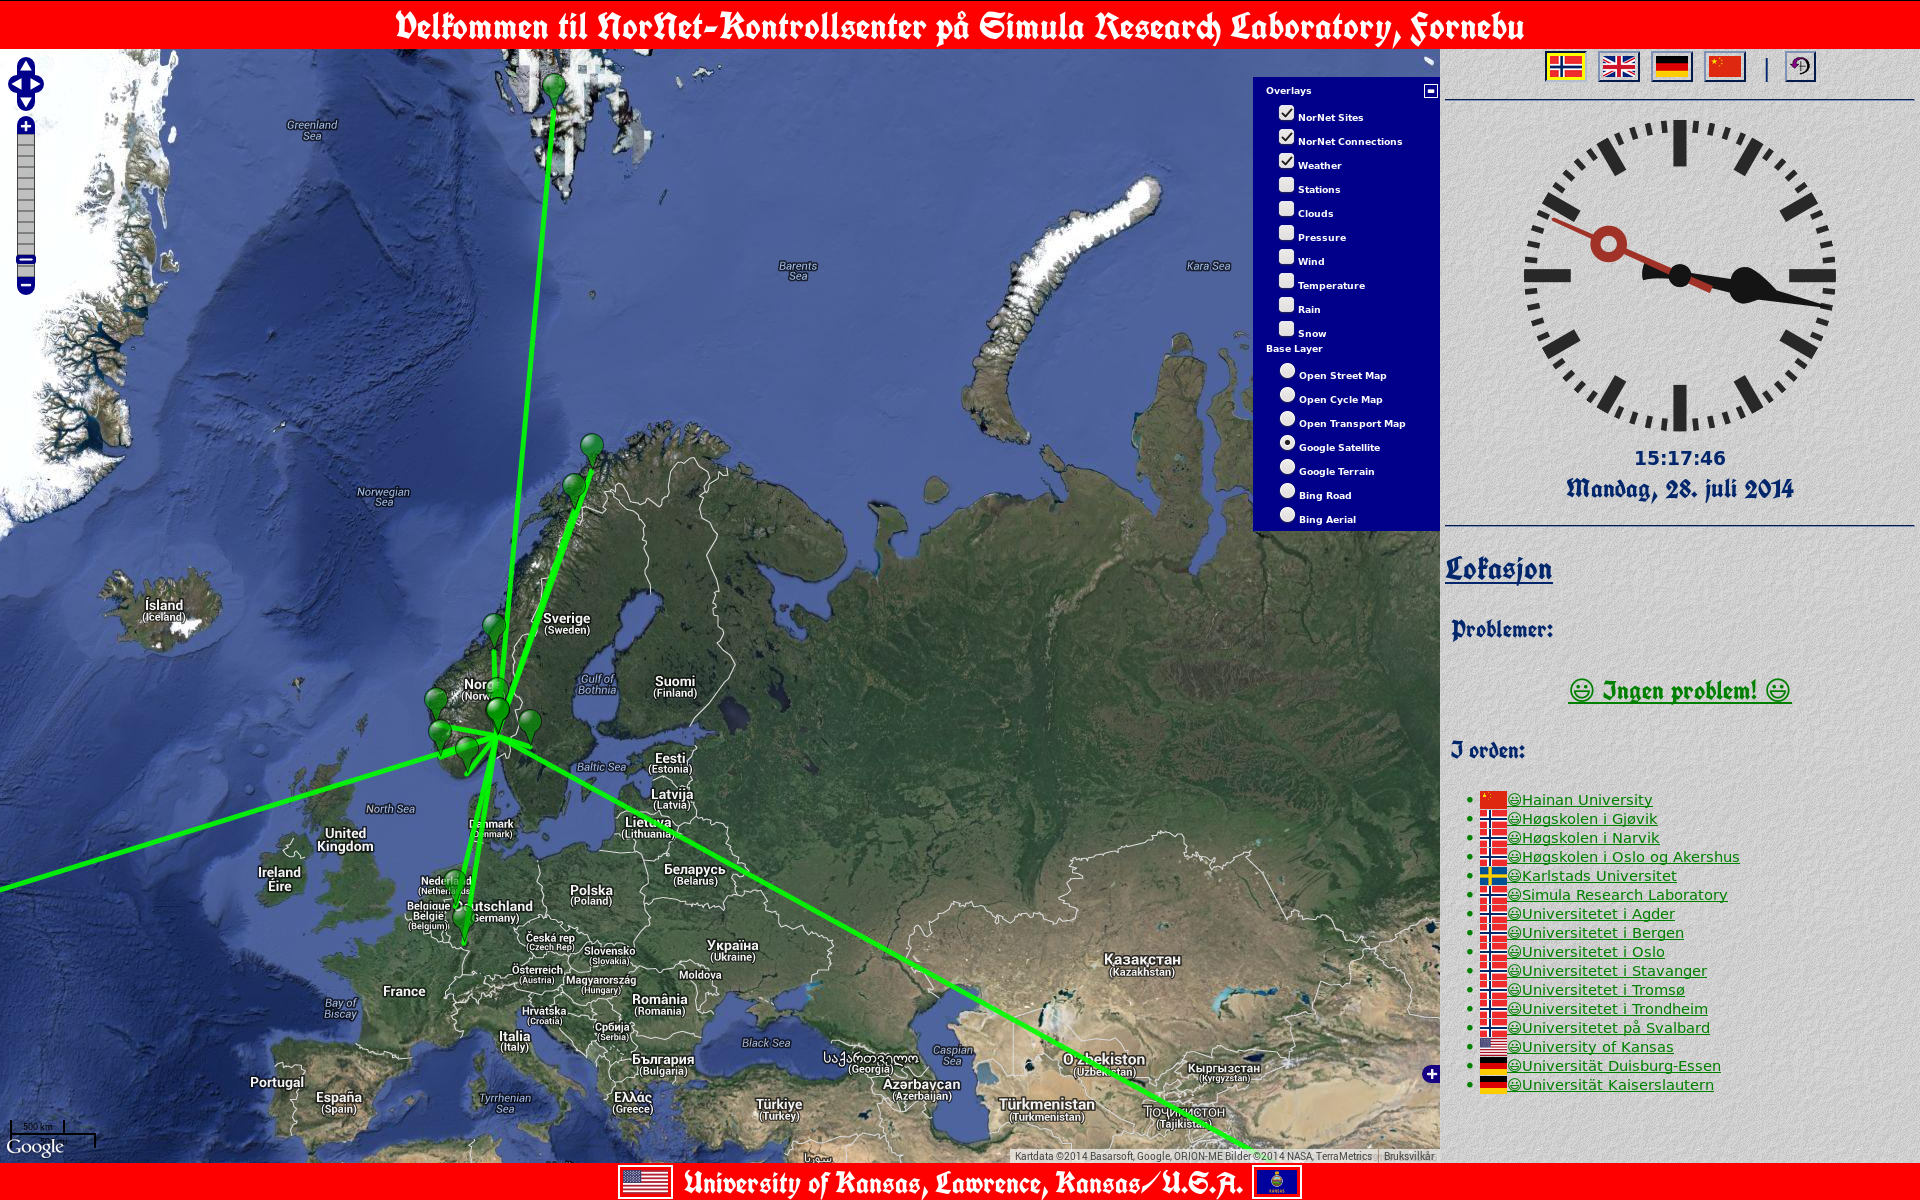
\includegraphics[width=0.98\columnwidth]{%
   Images/PDF/Kontrollsenteret.pdf}
\end{center}
\caption{\noun{NorNet-Kontrollsenter} -- A Screenshot of the Control Center Display}
\label{cap:Kontrollsenteret}
\end{figure*}
% %%%%%%%%%%%%%%%%%%%%%%%%%%%%%%%%%%%%%%%%%%%%%%%%%%%%%%%%%

In order to achieve the testbed availability described in Section~\ref{sec:Design}, tight monitoring is necessary to detect problems early and to trigger their resolution as soon as possible. The basis of our monitoring infrastructure is a \noun{Nagios}~\cite{NagiosCoreDocumentation} setup, which is deployed in a virtual machine at the Central Site. The ``Monitor'' package provides this functionality, based on the ``Node'' package (see Subsection~\ref{sub:The-Nodes}). \noun{Nagios} actively obtains the status of all components, e.g.\ the systems themselves with \noun{Ping} tests, and services like the PLC's web server by HTTP checks. Particularly, \noun{Nagios} allows a fine-granular configuration of warning and error conditions, as well as the extension to custom services (e.g.\ to check certain system-dependent status values by using SNMP) in form of plug-ins. Such plug-ins have been written to perform checks of sites and tunnels. The monitoring results are recorded by \noun{Nagios}; a web interface provides access for administrators.

While the web interface presents a very detailed and fine-grained view of \noun{NorNet Core}, a more illustrative view was intended to give a quick overview of the site statuses for both administrators and users of the testbed (i.e.\ the researchers). Therefore, we -- as a first step -- applied the \noun{NagMap}\footnote{\noun{NagMap}: \url{https://github.com/hecko/nagmap/}.} plug-in for \noun{Nagios}, which provided a map view of the \noun{NorNet Core} testbed. However, \noun{NagMap} just produced a quite simple projection of the sites and their connections (i.e.\ the tunnels) to a \noun{Google Maps}\footnote{\noun{Google Maps}: \url{https://maps.google.no/}.} satellite map. Particularly due to the fully-connected mesh topology of the tunnels (see Section~\ref{sec:Design}), the link view, however, became relatively confusing. Therefore, we have developed our own plug-in named \noun{NorNet-Kontrollsenter}.

\noun{NorNet-Kontrollsenter}\index{Kontrollsenteret}\index{NorNet-Kontrollsenter} uses \noun{Apache}/PHP~\cite{ApacheDoc} to access the recorded \noun{Nagios} status information. It then provides an HyperText Markup Language\nomenclature{HTML}{HyperText Markup Language}\index{HyperText Markup Language}~(HTML\index{HTML|see{HyperText Markup Language}}) page with the results. That is, the plug-in runs on the monitoring system itself. The results can then be accessed from a web server running on the same system, while a web browser on another machine can display the corresponding webpage (as shown in Figure~\ref{cap:Kontrollsenteret}). The returned web page with the results makes use of JavaScript, AJAX (Asynchronous JavaScript and XML) as well as SVG (Scalable Vector Graphics) with JavaScript to provide dynamic updates without having to reload the whole page. Furthermore, instead of tying the map display to a certain map service, we apply \noun{OpenLayers}~\cite{OpenLayersDoc}. It provides a service-independent mapping and layering library in JavaScript; the display can dynamically change between map services (currently, we apply 
\noun{Open Street Map}\footnote{\noun{Open Street Map}: \url{http://www.openstreetmap.org/}.},
\noun{Google Maps} and
\noun{Bing Maps}\footnote{\noun{Bing Maps}: \url{http://www.bing.com/maps/}.}). Furthermore, overlaying functionality is provided. That is, overlays like the \noun{Open Weather Map}\footnote{\noun{Open Weather Map}: \url{http://www.openweathermap.org/}.} overlay can add additional information to the map (in Figure~\ref{cap:Kontrollsenteret}: the current weather as well as clouds and precipitation forecasts). In the future, we plan to use this feature for more detailed network status information. Map services and the visibility of overlays can be changed interactively.

For improved visibility, we only display a connection to the Central Site (in green colour) if all tunnels of a site are working. Only non-working tunnels would result in yellow (warning level) or red (error level) coloured links between sites. Connections to not-yet-deployed sites are represented by grey, dashed lines.

Since the access to the monitoring results is browser-based, it is possible to run multiple browser instances simultaneously. We use this feature e.g.\ to display a map of the Norwegian mainland (see Figure~\ref{cap:Kontrollsenteret}) on a large screen as well as a map of Svalbard (more than 1,000~km north of the mainland) on a separate, small screen. The ``Display'' package extends the ``Node'' setup with configurations for such a display machine, by adding an X~server and the \noun{Firefox} web browser.


% -> mobility support in the future
% -> GUI Localisation



% ###########################################################################
\section{Testbed Deployment and Research Ideas}
% ###########################################################################

Currently, we are in the deployment phase of the sites~\cite{Karlstad2012}. That is, the hardware setup described in Subsection~\ref{sub:The-Sites} has been installed at 7~sites, with 3~further sites in the following weeks.

For the research part of \noun{NorNet Core}, there are obviously use cases for research on resilience (e.g.\ in the context of RSerPool~\cite{IJIIDS2010,Dre2006,rfc-rserpool-overview}, etc.). Furthermore, there is a strong interest in using the testbed in the context of multi-path transport performance with MPTCP~\cite{RBP+11} and CMT-SCTP~\cite{PAMS2012}, as well as for congestion control evaluations~\cite{Globecom2013,ICC2012,YWY08a} in that context. Particularly, there is a growing interest in CMT-SCTP, since \emph{Real-Time Collaboration on the World Wide Web}~(RTCWEB)~\cite{draft-ietf-rtcweb-overview} is based on SCTP. RTCWEB is a framework for browser-to-browser multimedia communications (e.g.\ video conferencing) that is currently under standardisation in the IETF and therefore a very hot research topic. With SCTP being deployed by possibly billions of web browsers on frequently multi-homed endpoints (e.g.\ tablet PCs and smartphones with 3G and WLAN interfaces), the usage of multi-path transport might become very tempting. 



% @@@@@@@@@@@@@@@@@@@@@@@@@@@@@@@@@@@@@@@@@@@@@@@@@@@@@@@@@@@@@@@@@@@@@@@@@@@
\chapter{Getting Access}
\label{cha:Getting-Access}
% @@@@@@@@@@@@@@@@@@@@@@@@@@@@@@@@@@@@@@@@@@@@@@@@@@@@@@@@@@@@@@@@@@@@@@@@@@@

In this chapter, the user part of accessing and using \noun{NorNet Core} is described.
% The maintenance part will be described in Chapter~\ref{cha:Maintenance}.


% ###########################################################################
\section{User Accounts}
\label{sec:User-Accounts}
% ###########################################################################

% %%%%%%%%%%%%%%%%%%%%%%%%%%%%%%%%%%%%%%%%%%%%%%%%%%%%%%%%%
\begin{table}
\begin{center}
\begin{tabular}{|l||l|l|}
 \hline
 Server             & User Name  & Password \\ \hline
 \hline
 \href{ssh://gatekeeper.nntb.no}{gatekeeper.nntb.no}\index{gatekeeper.nntb.no}~(Gatekeeper) & ola                                                               & some-secret-password \\ \hline
 \href{https://plc.simula.nornet}{plc.simula.nornet}\index{plc.simula.nornet}~(PLC)         & \href{mailto:ola.nordmann@example.com}{ola.nordmann@example.com}  & another-password     \\ \hline
\end{tabular}
\end{center}
\caption{An Example Accounts Table}
\label{tbl:An-Example-Accounts-Table}
\end{table}
% %%%%%%%%%%%%%%%%%%%%%%%%%%%%%%%%%%%%%%%%%%%%%%%%%%%%%%%%%

A new \noun{NorNet Core} user will at least receive the following accounts:
\begin{itemize}
 \item The Gatekeeper account providing access to a Linux machine that is connected to \noun{NorNet Core} and the outside Internet.
 \item The PLC account providing access to the PLC (see Subsection~\ref{sub:The-Testbed-Management}). Note, that the PLC user name \emph{must} be a valid e-mail address of the user.
\end{itemize}
Possibly, further accounts will be provided, e.g.\ for web server, wiki server, etc.. Such accounts are optional and only provided when needed.
Table~\ref{tbl:An-Example-Accounts-Table} shows an example for the user Ola Nordmann.
Note, that users are \emph{required} to change their initial passwords as soon as possible!



% ###########################################################################
\section{Getting Access into the \noun{NorNet Core} Network}
\label{sec:Access-into-NorNet-Core-Network}
% ###########################################################################

A \noun{NorNet Core} user needs access into the \noun{NorNet Core} network. The possibilities for such accesses are introduced in the following subsections.


% ===========================================================================
\subsection{The Gatekeeper}
\label{sub:The-Gatekeeper}
% ===========================================================================

The Gatekeeper server\index{Gatekeeper} \href{ssh://gatekeeper.nntb.no}{gatekeeper.nntb.no}\index{gatekeeper.nntb.no}\footnote{\href{ssh://gatekeeper.nntb.no}{gatekeeper.nntb.no}\index{gatekeeper.nntb.no} is actually an alias for the server \href{ssh://oesthorn.nntb.no}{oesthorn.nntb.no}\index{oesthorn.nntb.no}).}
% to be explained in Section~\ref{sec:The-Gatekeeper}.}
provides the simplest form of access to the \noun{NorNet Core} network. It is just a Linux machine that is connected to the \noun{NorNet Core} network as well as to the outside Internet. SSH\index{Secure Shell} can be used to access this machine. In the following, some useful commands that are provided by standard Linux distributions are explained. Note, that access to the Gatekeeper is not restricted to Linux. In fact, any operating system with appropriate tools (SSH, etc.) can be used as well.

The following examples give a short overview of what is possible with SSH. Note, that they are not meant to be complete. Refer to the manual page of \texttt{ssh}\footnote{\texttt{ssh} manual page: \texttt{\href{man:ssh}{man ssh}}.} and various SSH tutorials in the Internet for further information.


% ---------------------------------------------------------------------------
\subsubsection{Using Secure Shell}
\label{subsub:Gatekeeper-Using-SSH}
% ---------------------------------------------------------------------------

An SSH remote shell connection to the Gatekeeper server\index{Gatekeeper!Secure Shell} can be established e.g.\ by the \texttt{ssh}\index{ssh} command:
\begin{lstlisting}
ssh ola@gatekeeper.nntb.no
\end{lstlisting}
for user ``ola''. Of course, the user has to set his own Gatekeeper username here. For login, the corresponding  is required. Key-based authentication will be explained in Subsubsection~\ref{subsub:Key-Based-Authentication}.


% ---------------------------------------------------------------------------
\subsubsection{Changing the Password}
% ---------------------------------------------------------------------------

Once logged in the the Gatekeeper server, the user can change the password\index{Password}\index{Gatekeeper!Password Change} with the \texttt{passwd} command. It asks for the old password and twice for the new one. If both inputs of the new password are equal, the password is updated. The user is required to chose a ``good'' password for the Gatekeeper, since it is exposed to the outside Internet.


% ---------------------------------------------------------------------------
\subsubsection{Using Secure Copy}
% ---------------------------------------------------------------------------

Secure Copy\nomenclature{SCP}{Secure Copy}\index{Secure Copy}~(SCP\index{SCP|see{Secure Copy}}) uses SSH to transfer files between machines, i.e.\ it is possible to copy files from the local machine to the Gatekeeper\index{Gatekeeper!Secure Copy} and vice versa. The corresponding command is named \texttt{scp}\index{scp}.

To copy a file \texttt{test.data} from the local machine to the Gatekeeper server, use for example:
\begin{lstlisting}
scp test.data ola@gatekeeper.nntb.no:
\end{lstlisting}
Note the colon (i.e.\ ``:'')! Without this colon, ssh would behave like a local file copy (i.e.\ \texttt{cp}\index{cp}) and just create a local copy of \texttt{test.data} with name \text{ola@gatekeeper.nntb.no}. \texttt{scp} will store the file in the home directory (the default place) of the Gatekeeper server. A different directory can be specified after the colon, e.g.\ \texttt{directory/subdirectory} (note, that these directories must exist):
\begin{lstlisting}
scp test.data ola@gatekeeper.nntb.no:directory/subdirectory/
\end{lstlisting}
It is furthermore possible to provide a file name for the destination (e.g.\ \texttt{my-first-test.data}):
\begin{lstlisting}
scp test.data ola@gatekeeper.nntb.no:directory/my-first_test.data
\end{lstlisting}
\texttt{scp} can also copy complete directories, by using the ``-r'' option for a recursive copy:
\begin{lstlisting}
scp -r test-directory ola@gatekeeper.nntb.no:
\end{lstlisting}
This will copy the whole directory \texttt{test-directory}, including all of its subdirectories, to the Gatekeeper.

Similarly, the reverse direction -- i.e.\ from the Gatekeeper to the local machine -- can be handled as well:
\begin{lstlisting}
scp ola@gatekeeper.nntb.no:test.data .
scp ola@gatekeeper.nntb.no:test.data some-local-directory/
scp -r ola@gatekeeper.nntb.no:my-test-directory/ .
\end{lstlisting}
Of course, copying from a remote to another remote machine would work as well.
For further possibilities, also see the manual page of \texttt{scp}\footnote{\texttt{scp} manual page: \texttt{\href{man:scp}{man scp}}.}.


% ---------------------------------------------------------------------------
\subsubsection{Using Remote File Synchronisation}
% ---------------------------------------------------------------------------

SCP only copies files and directories. When working with \noun{NorNet Core} experiment results, it becomes handy to synchronise files and directories, i.e.\ to just transfer data that needs to be transferred. This functionality is provided by the texttt{rsync}\index{rsync} command\index{Gatekeeper!Remote Synchronisation}. See also the manual page of \texttt{rsync}\footnote{\texttt{rsync} manual page: \texttt{\href{man:rsync}{man rsync}}.} for details.

In order to synchronise the directory \texttt{experiment1/results/} from the Gatekeeper to the local machine, use for example:
\begin{lstlisting}
rsync -a -v -z --partial --progress --delete \
 ola@gatekeeper.nntb.no:experiment1/results/ experiment1/results/
\end{lstlisting}
The following options are of interest:
\begin{itemize}
 \item ``-a'': recursive synchronisation.
 \item ``-v'': verbose output.
 \item ``-z'': use compression for improving the transfer speed over slow connections. However, it comes of course at the cost of increased CPU utilisation.
 \item ``-\--partial'': allow to resume a file transfer after interruption. For example, having transferred 99\% of 1~GiB just needs the transfer the remaining 1\% after aborting and restarting \texttt{rsync}. Otherwise, the transfer of this file would restart from scratch.
 \item ``-\--progress': shows the progress of the transfer.
 \item ``-\--delete'': deletes files that are not existing any more in the source directory. Warning: this option may be disastrous when mistakenly providing the wrong destination (e.g.\ the user's home directory). Use this option with care!
\end{itemize}

Similarly, data can be synchronised from the local machine to the Gatekeeper:
\begin{lstlisting}
rsync -a -v -z --partial --progress experiment1/ \
 ola@gatekeeper.nntb.no:experiment1/
\end{lstlisting}


% ---------------------------------------------------------------------------
\subsubsection{Configuring Key-Based Authentication}
\label{subsub:Key-Based-Authentication}
% ---------------------------------------------------------------------------

Instead of typing the password for login each time, the user can also create a SSH public/private key pair on the local machine (i.e.\ the machine used to access the Gatekeeper server). By storing the public key on the Gatekeeper server in \texttt{.ssh/authorized\_keys}, the user can use his private key to authenticate to the Gatekeeper instead of using his password. This is particularly useful when using SSH in scripts.

To create a public/private key pair, the command \texttt{ssh-keygen}\index{ssh-keygen} is used:
\begin{lstlisting}
ssh-keygen -P "" -f ~/.ssh/gatekeeper
\end{lstlisting}
The following options are of interest:
\begin{itemize}
 \item ``-P'': specifies the passphrase for the private key. "" sets no passphrase; this is necessary to use the key in scripts later.
 \item ``-f'': provides the output file prefix. In this case, the private key will be stored in \texttt{\textasciitilde/.ssh/gatekeeper} and the corresponding public key in \texttt{\textasciitilde/.ssh/gatekeeper.pub}.
\end{itemize}
Also see the manual page\footnote{\texttt{ssh-keygen} Manual Page \href{man:ssh-keygen}{\texttt{man ssh-keygen}}.} of \texttt{ssh-keygen} for further options.


The public key (in this example: \texttt{\textasciitilde/.ssh/gatekeeper.pub}) is just a text file with one long line. It can be displayed e.g.\ with:
\begin{lstlisting}
cat ~/.ssh/gatekeeper.pub
\end{lstlisting}
It should be something like ``ssh-rsa <characters and numbers> <user@host>''.

To use this public key for authentication, log into the Gatekeeper and append the key line to the file \texttt{\textasciitilde/.ssh/authorized\_keys}. This can e.g.\ by done by an arbitrary text editor that is available on the Gatekeeper, e.g.\
\texttt{emacs}\index{emacs},
\texttt{joe}\index{joe},
\texttt{nano}\index{nano} or
\texttt{vi}\index{vi}. If the file \texttt{\textasciitilde/.ssh/authorized\_keys} does not yet exist, it can just be created. After creating the file, it is necessary to check the access permissions with \texttt{chmod}\index{chmod}:
\begin{lstlisting}
chmod 600 ~/.ssh/authorized_keys
\end{lstlisting}
This ensures that only the owner (and root, of course) can read or modify it. See also the manual page\footnote{\texttt{chmod} Manual Page \href{man:chmod}{\texttt{man chmod}}.} of \texttt{chmood}. Note, that without secure access permissions, the SSH daemon will refuse to apply the key configuration!

The Gatekeeper should now be ready for public/private key-based authentication. From the local machine, now use
\begin{lstlisting}
ssh -i ~/.ssh/gatekeeper ola@gatekeeper.nntb.no:
\end{lstlisting}
to log into the Gatekeeper. ``-i'' specifies the private key that SSH should use for authentication. If everything is working, \texttt{ssh} should log into the Gatekeeper without need for entering the password. Note, that SSH may not complain if the private key is not found. Instead, it will try password-based authentication. If this is the case, check the provided file name of the private key.


% ---------------------------------------------------------------------------
\subsubsection{Tunnelling TCP Connections}
\label{subsub:Tunnelling-TCP-Connections}
% ---------------------------------------------------------------------------

SSH provides the feature of tunnelling TCP connections via an SSH session. That is, for a given TCP port on the local machine, SSH tunnels the traffic to the remote SSH endpoint (here: the Gatekeeper). From there, it is forwarded to the given destination.  For \noun{NorNet Core}, this is particularly useful to get access to the PLC (to be explained in Section~\ref{sec:The-PLC}), the Monitor server (to be explained in Section~\ref{sec:Kontrollsenteret}) and the Performance Server (to be explained in Section~\ref{sec:PerfMon}):
\begin{lstlisting}
ssh ola@gatekeeper.nntb.no \
 -L 2000:plc.simula.nornet:443 \
 -L 2001:monitor.simula.nornet:80 \
 -L 2002:perfmon1.simula.nornet:80
\end{lstlisting}
This code example does the following:
\begin{itemize}
 \item An SSH connection is established to the Gatekeeper server \href{ssh://gatekeeper.nntb.no}{gatekeeper.nntb.no}\index{gatekeeper.nntb.no}, as explained in Subsubsection~\ref{subsub:Gatekeeper-Using-SSH}.
 
 \item TCP port~2000 of the local machine (i.e.\ the machine running this command) is forwarded via the Gatekeeper to port~443 of the PLC server \href{https://plc.simula.nornet}{plc.simula.nornet}\index{plc.simula.nornet}. Note, that \href{https://plc.simula.nornet}{plc.simula.nornet}\index{plc.simula.nornet} is the DNS name of the PLC. Since the Gatekeeper uses the \noun{NorNet Core} DNS service, it can resolve this \noun{NorNet}-internal name (see Subsubsection~\ref{subsub:Tunnelbox-Name-Resolution}).
 
 \item Similarly, TCP port~2001 of the local machine is forwarded to port~80 of the Monitor server \href{http://monitor.simula.nornet}{monitor.simula.nornet}\index{monitor.simula.nornet}.

 \item Finally, TCP port~2002 of the local machine is forwarded to port~80 of the Performance server \href{http://perfmon1.simula.nornet}{perfmon1.simula.nornet}\index{perfmon1.simula.nornet}.
\end{itemize}
By establishing a TCP connection to port~2000, port~2001 or port~2002 of the local machine, the user can now access the \noun{NorNet}-internal services of the PLC, the Monitor server or Performance server (to be explained later in Section~\ref{sec:The-PLC}, Section~\ref{sec:Kontrollsenteret} and Section~\ref{sec:PerfMon}).

% %%%%%%%%%%%%%%%%%%%%%%%%%%%%%%%%%%%%%%%%%%%%%%%%%%%%%%%%%
\begin{algorithm}
\lstinputlisting{CodeSnippets/Gatekeeper.sh}
\caption{A Gatekeeper Access Script Example}
\label{lst:Gatekeeper-Access-Script-Example}
\end{algorithm}
% %%%%%%%%%%%%%%%%%%%%%%%%%%%%%%%%%%%%%%%%%%%%%%%%%%%%%%%%%

Since the establishment of the port forwarding above is a recurring task for almost all \noun{NorNet Core} users, it is strongly recommended to write a small script to perform this task. An example is provided in Listing~\ref{lst:Gatekeeper-Access-Script-Example}.



% ===========================================================================
\subsection{Getting Physical Access}
\label{sub:Getting-Physical-Access}
% ===========================================================================

A user can get physical access to \noun{NorNet Core} by connecting devices to his local site's \noun{NorNet Core} switch (see Figure~\ref{cap:The-Site-Setup}). This ensures easy access and provides the lowest latency and greatest flexibility.
The local network provides automatic IPv4 configuration of the primary ISP by the Dynamic Host Configuration Protocol\nomenclature{DHCP}{Dynamic Host Configuration Protocol}\index{Dynamic Host Configuration Protocol}~(DHCP\index{DHCP|see{Dynamic Host Configuration Protocol}}, \cite{RFC2131,RFC2132}). Note, that DHCP does \emph{not} provide addresses for further ISPs. DHCP will also provide the DNS address (i.e.\ the tunnelbox, see Subsubsection~\ref{subsub:Tunnelbox-Name-Resolution}) so that \noun{NorNet}-internal names can be resolved. Note furthermore, that TCP access with port~80 to non-local endpoints is proxied via the local tunnelbox's Squid proxy (transparent proxy), in order to provide caching.

For IPv6, addresses for all ISPs are be provided by stateless auto-configuration via Internet Control Message Protocol version~6\nomenclature{ICMPv6}{Internet Control Message Protocol version~6}\index{Internet Control Message Protocol version~6}~(ICMPv6\index{ICMPv6|see{Internet Control Message Protocol version~6}}, \cite{RFC4443}).

Note, that dynamic configuration is intended for short-term usage. For long-term usage of devices within the \noun{NorNet Core} network, it is required to configure permanent address mappings for DHCP as well as DNS names. See ******* for the maintenance details!



% ===========================================================================
\subsection{The Virtual Private Network Access}
\label{sub:The-VPN-Access}
% ===========================================================================

An access to the \noun{NorNet Core} network via Virtual Private Network\nomenclature{VPN}{Virtual Private Network}\index{Virtual Private Network}~(VPN\index{VPN|see{Virtual Private Network}}) is planned but not yet implemented.



% ###########################################################################
\section{The PLC}
\label{sec:The-PLC}
% ###########################################################################

The PLC\index{PlanetLab Central} user interface used for \noun{NorNet Core} is mostly based on the upstream \noun{PlanetLab}~\cite{PR06} software. It is therefore only very briefly introduced here.


% ===========================================================================
\subsection{Accessing the PLC Web Interface}
\label{sub:Accessing-the-PLC-Web-Interface}
% ===========================================================================

First, it is necessary to get access to the PLC web interface via a web browser. There are two possibilities:
\begin{itemize}
 \item \url{https://plc.simula.nornet}:
 In case of connection to the local \noun{NorNet Core} network including its DNS service, the web browser can directly connect to the PLC.
 
 \item \url{https://localhost:2000}:
 If access to the \noun{NorNet Core} network is only available via the Gatekeeper server, the SSH port forwarding -- as described in Subsubsection~\ref{subsub:Tunnelling-TCP-Connections} -- can be used. Then, if using the settings described there, the web browser connects to the local machine's port~2000. This port is forwarded, via SSH and the Gatekeeper server, to the PLC.
\end{itemize}

The PLC uses a self-signed Transport Layer Security\nomenclature{TLS}{Transport Layer Security}\index{Transport Layer Security}~(TLS\index{TLS|see{Transport Layer Security}}) certificate. When establishing a connection for the first time, this certificate has to be accepted for the web browser.


Currently, the management of sites and nodes (particularly e.g.\ adding sites or nodes) is made directly by the \noun{NorNet Core} staff at the Simula Research Laboratory.
The PLC web interface can be used by \noun{NorNet Core} users to perform the following tasks:
\begin{itemize}
 \item Managing the PLC account,
 \item Viewing sites and nodes information,
 \item Managing slices.
\end{itemize}
These tasks will be explained in the following subsections.


% ===========================================================================
\subsection{Managing the User Account}
\label{sub:Managing-the-Account}
% ===========================================================================

% %%%%%%%%%%%%%%%%%%%%%%%%%%%%%%%%%%%%%%%%%%%%%%%%%%%%%%%%%
\begin{figure*}
\begin{center}
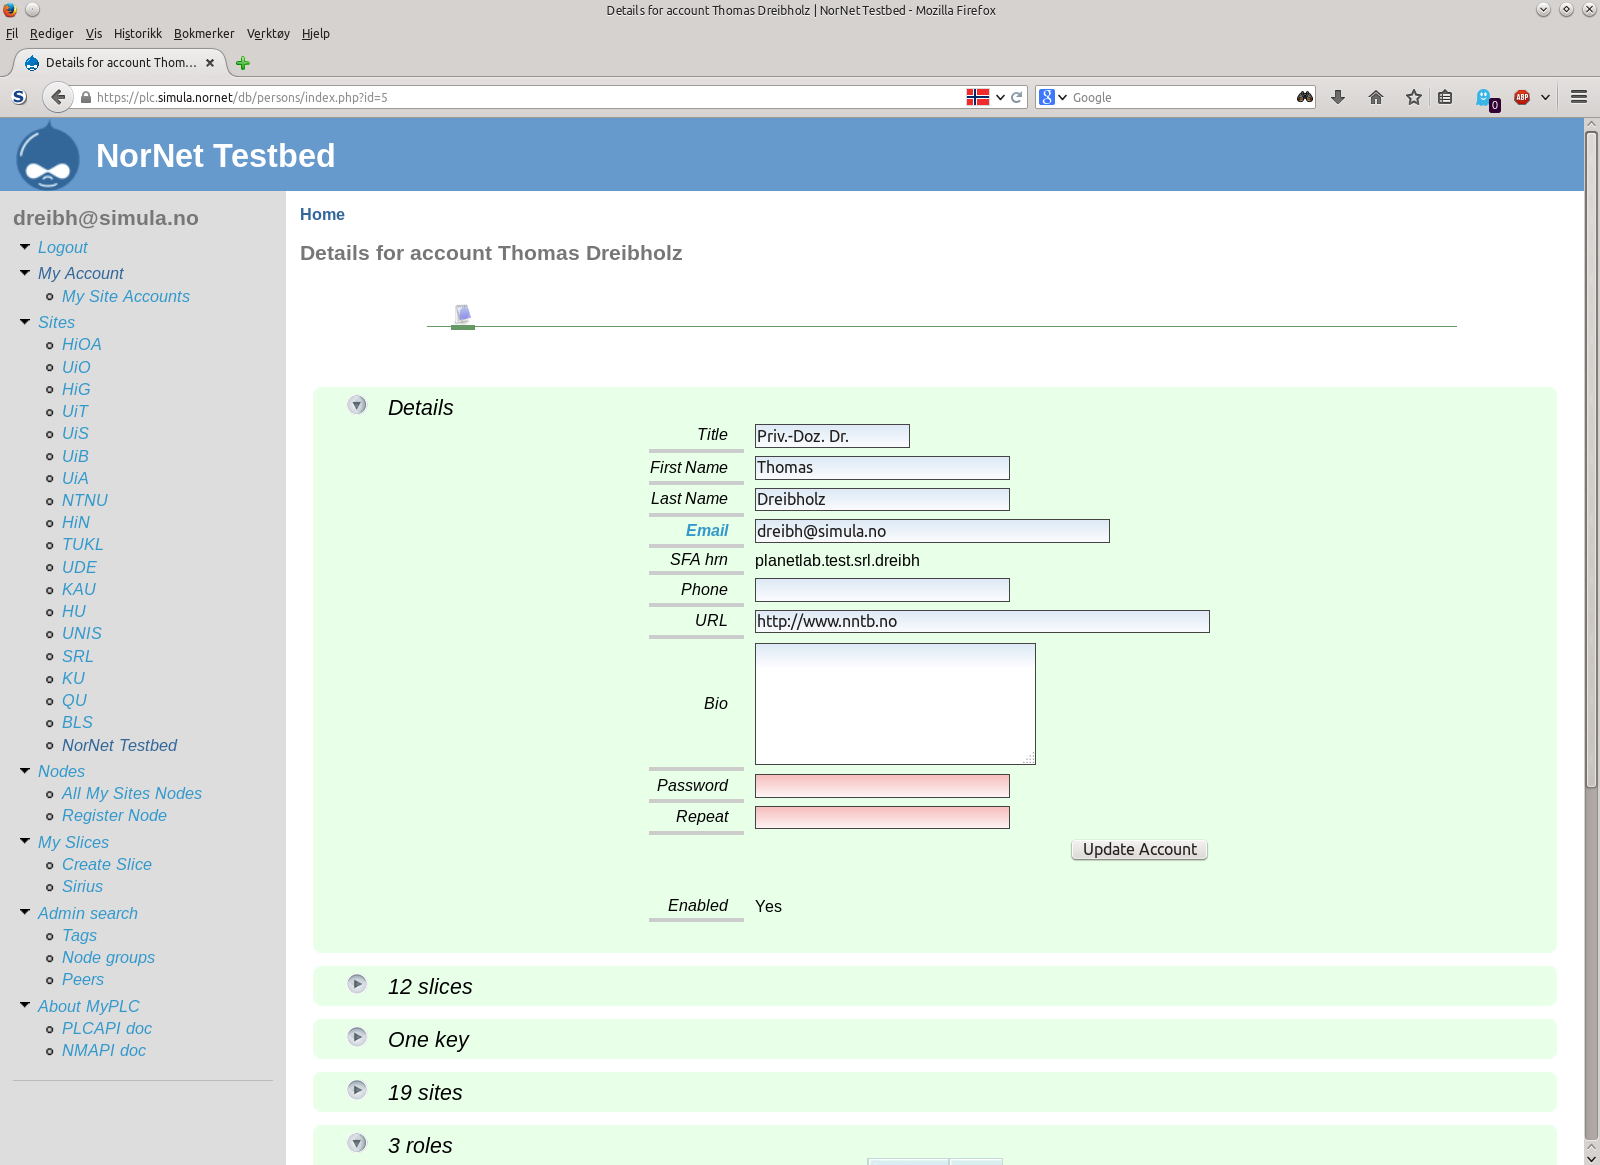
\includegraphics[width=0.95\columnwidth]{Images/PDF/Screenshot-PLC-Account-Details1.pdf}
\end{center}
\caption{The PLC: My Account $\rightarrow$ Details}
\label{cap:PLC-Account-Details-User}
\end{figure*}
% %%%%%%%%%%%%%%%%%%%%%%%%%%%%%%%%%%%%%%%%%%%%%%%%%%%%%%%%%

The own account is managed under ``My Account''. Figure~\ref{cap:PLC-Account-Details-User} shows an example screenshot. Particularly, the user can revise title, first and last name and biography information. Also, the user can change his own password. Since the PLC is used my many users and misuse of an account may affect the whole testbed, all user are \emph{required} to choose ``good'' passwords!

% %%%%%%%%%%%%%%%%%%%%%%%%%%%%%%%%%%%%%%%%%%%%%%%%%%%%%%%%%
\begin{figure*}
\begin{center}
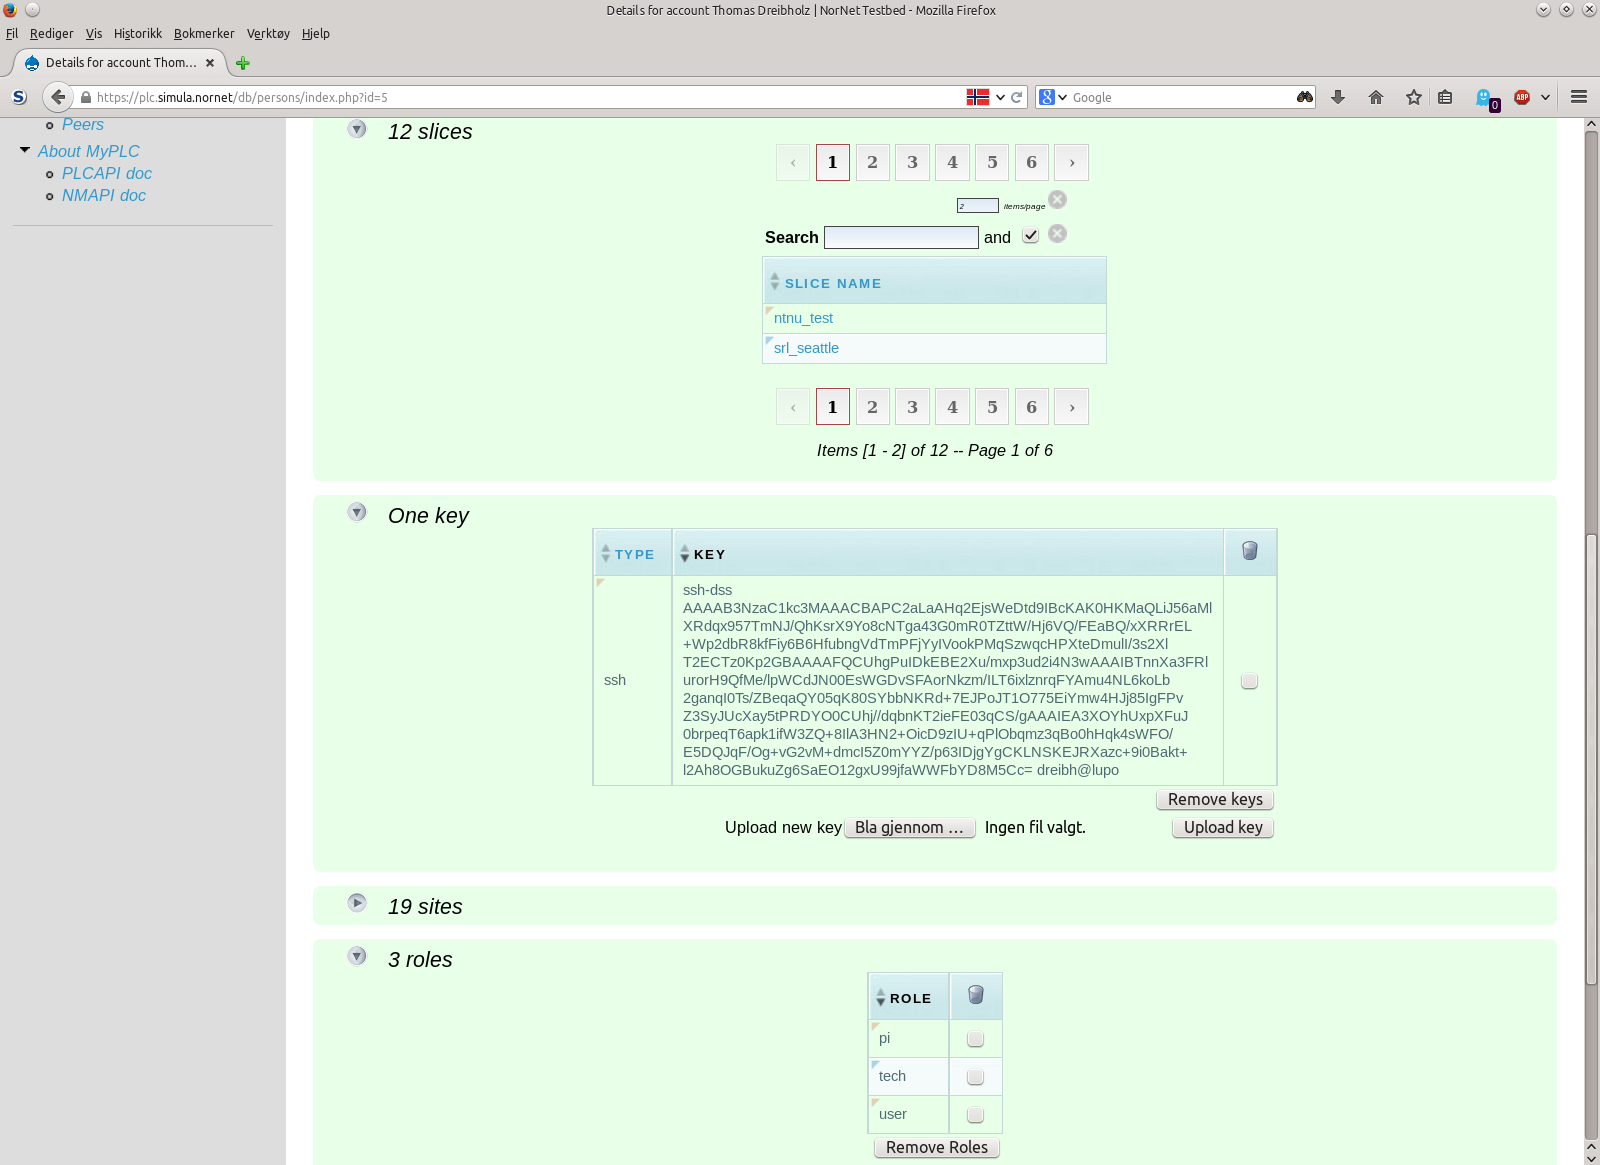
\includegraphics[width=0.95\columnwidth]{Images/PDF/Screenshot-PLC-Account-Details2.pdf}
\end{center}
\caption{My Account $\rightarrow$ Slices, Key and Roles}
\label{cap:PLC-Account-Details-Key-and-Roles}
\end{figure*}
% %%%%%%%%%%%%%%%%%%%%%%%%%%%%%%%%%%%%%%%%%%%%%%%%%%%%%%%%%

Further information under ``My Account'' provides mappings of the user to one or more \noun{NorNet Core} sites, mappings to slices and user roles. Since these functionalities are equal to \noun{PlanetLab}~\cite{PR06}, they are not introduced in detail here. Crucial for the access to \noun{NorNet Core} slivers is of course to provide an own SSH public key to the PLC. Like for using the Gatekeeper server with private/public key-based authentication (as introduced in Subsubsection~\ref{subsub:Key-Based-Authentication}), key-based authentication is used for accessing slivers. That is, the PLC provides the users' public keys to research nodes. The research nodes configure \texttt{authorized\_keys} with these keys for the slivers of the users. Then, the users can use their private key to authenticate to their slivers on the research nodes.

The own SSH public key can be uploaded in the ``Key'' tab of the ``My Account'' section, as shown in Figure~\ref{cap:PLC-Account-Details-Key-and-Roles}. Note, that multiple keys can be provided here. The PLC user interface currently only supports a single key for authentication. Therefore, only the first key will be used. However, the PLC does not display any warning when having uploaded multiple keys! It is therefore strongly recommended to not have more than one key in the interface. A further pitfall for new users is trying to upload their private key here. The PLC will in this case complain about the key length, but not about using a private key.

After upload of the public key, it may take up to about 1~hour until the new key gets distributed to all \noun{NorNet Core} research nodes. Key updates are made by the nodes in random intervals (by the Node Manager),
% -- to be described in Section~\ref{sec:Node-Manager}),
i.e.\ changes made in the PLC web interface are not applied immediately!


% ===========================================================================
\subsection{Sites}
\label{sub:Sites}
% ===========================================================================

% %%%%%%%%%%%%%%%%%%%%%%%%%%%%%%%%%%%%%%%%%%%%%%%%%%%%%%%%%
\begin{figure*}
\begin{center}
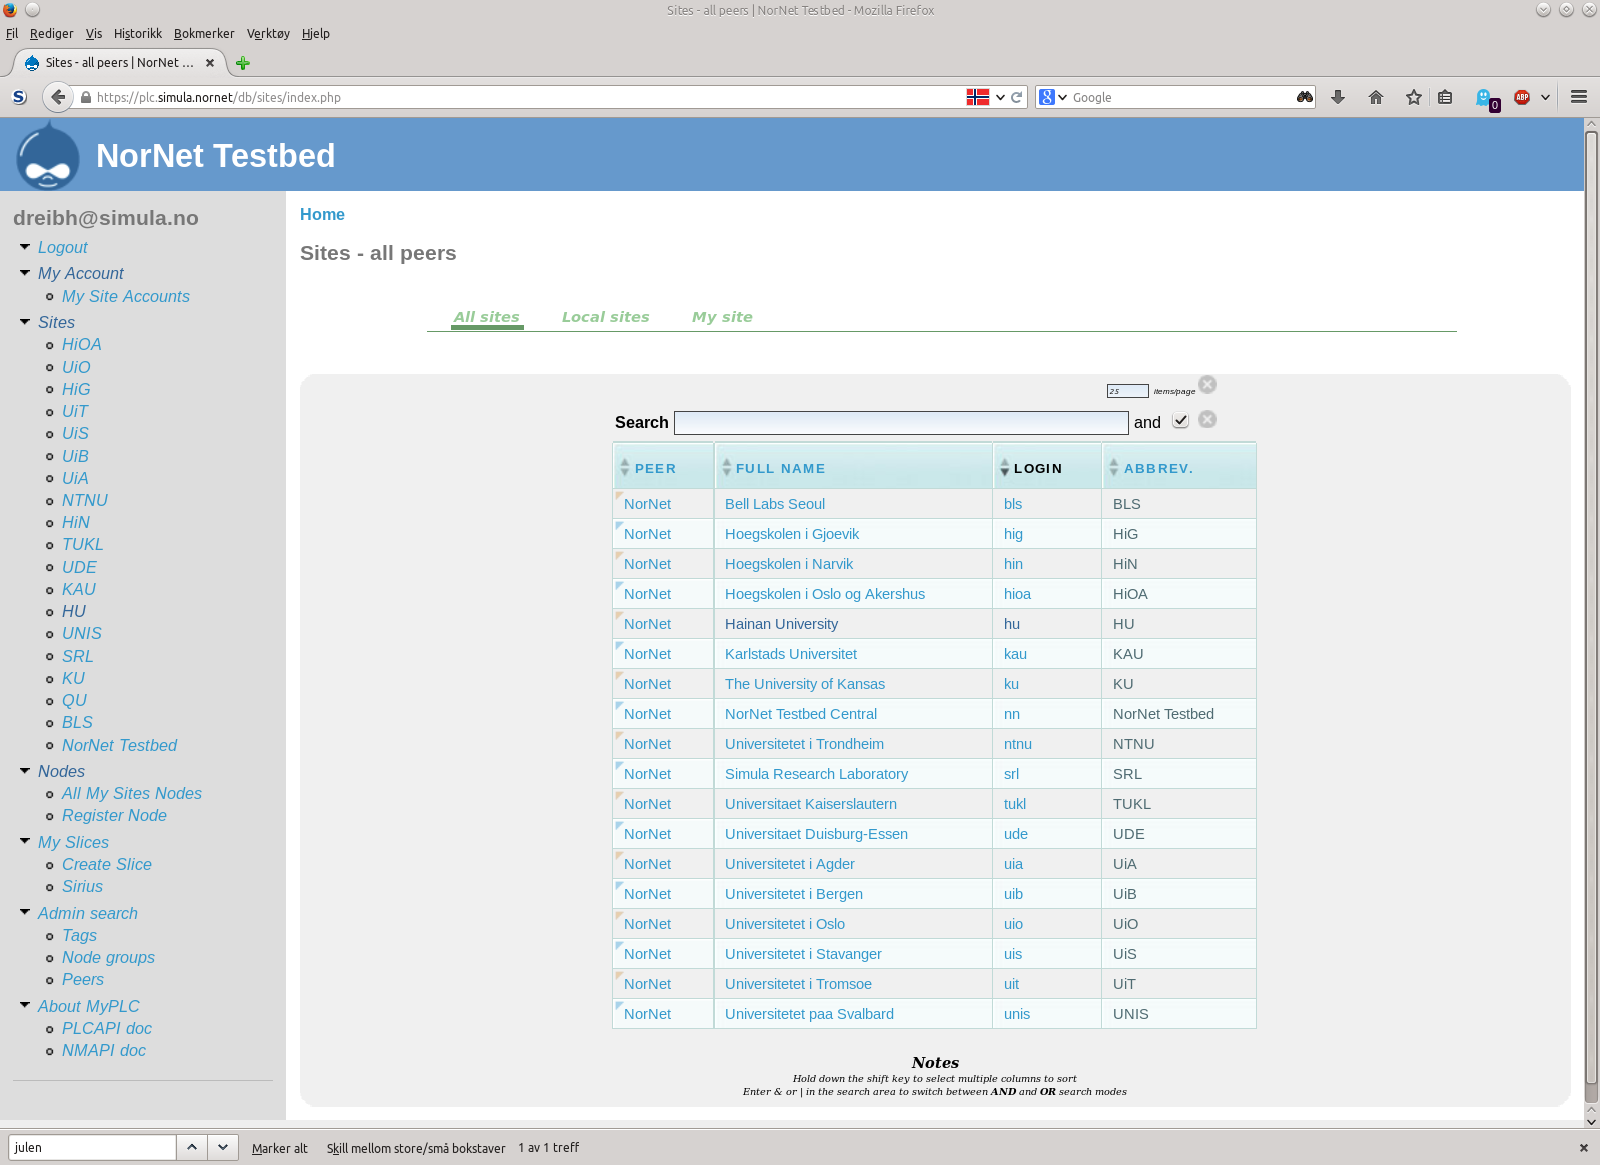
\includegraphics[width=0.95\columnwidth]{%
   Images/PDF/Screenshot-PLC-Sites.pdf}
\end{center}
\caption{Sites}
\label{cap:PLC-Sites}
\end{figure*}
% %%%%%%%%%%%%%%%%%%%%%%%%%%%%%%%%%%%%%%%%%%%%%%%%%%%%%%%%%

Information about the available \noun{NorNet Core} sites\index{Sites} are provided under the ``Sites'' section, as shown in Figure~\ref{cap:PLC-Sites}. The overview table just contains the sites' full names (e.g.\ Simula Research Laboratory\index{Simula Research Laboratory}) and abbreviation (e.g.\ SRL). Details on a site can be found by clicking on a site's label.

% %%%%%%%%%%%%%%%%%%%%%%%%%%%%%%%%%%%%%%%%%%%%%%%%%%%%%%%%%
\begin{figure*}
\begin{center}
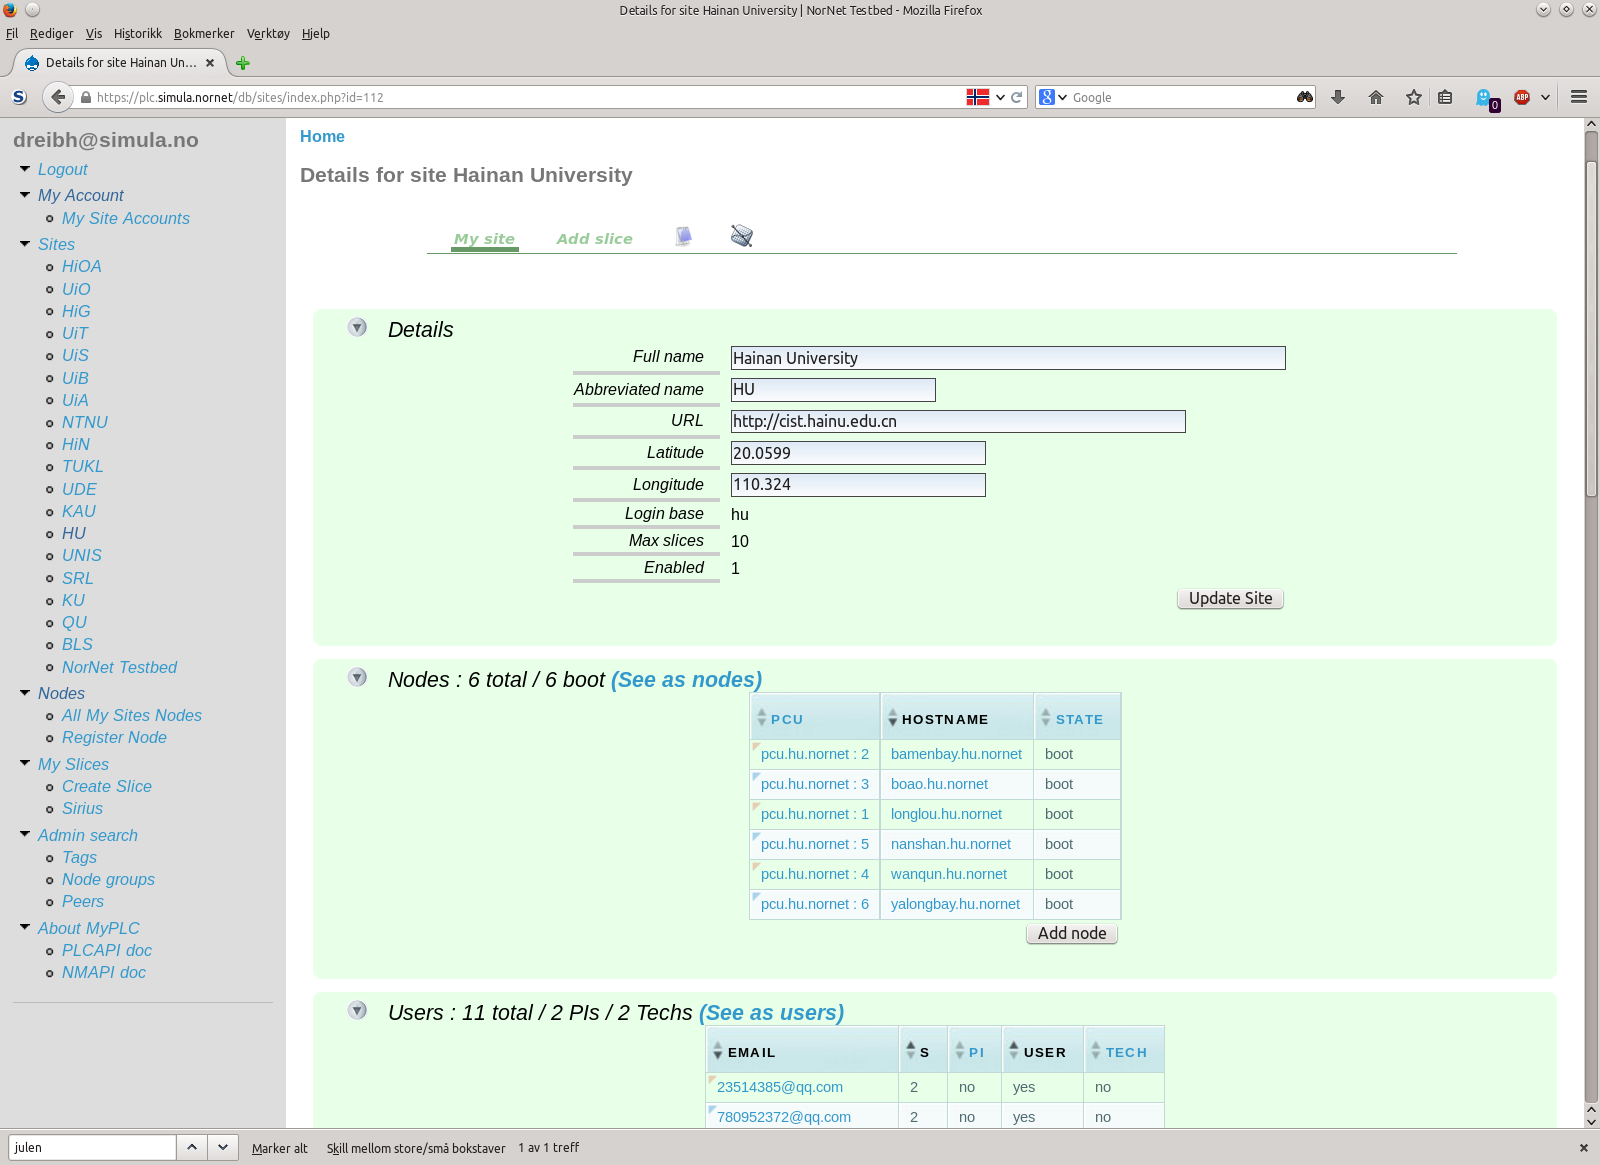
\includegraphics[width=0.95\columnwidth]{%
   Images/PDF/Screenshot-PLC-Sites-HU.pdf}
\end{center}
\caption{Sites $\rightarrow$ Hainan University~(HU)}
\label{cap:PLC-Sites-HU}
\end{figure*}
% %%%%%%%%%%%%%%%%%%%%%%%%%%%%%%%%%%%%%%%%%%%%%%%%%%%%%%%%%

Figure~\ref{cap:PLC-Sites-HU} presents the detailed site information view for the Hainan University\index{Hainan University} site. Particularly, it contains data such as the site's URL\nomenclature{URL}{Uniform Resource Locator}\index{Uniform Resource Locator}\index{URL|see{Uniform Resource Locator}}, the location, the research nodes and the users at a site. \noun{NorNet}-specific information is stored in custom tags:
\begin{itemize}
 \item ``nornet\_is\_managed\_site''\index{nornet\_is\_managed\_site}: Denotes whether the site is a \noun{NorNet Core}-managed site~(``1'') or not~(``0''). \noun{NorNet Core}-managed sites are assumed to be modified by scripts on the PLC server (by the \noun{NorNet Core} staff) only. Therefore, the configuration of the sites should \emph{not} be changed in the PLC web interface (even if the user's role allows to do this) to avoid misconfiguration!

 \item ``nornet\_site\_utf8''\index{nornet\_site\_utf8}: The site name in UTF-8\footnote{Universal Character Set Transformation Format -- 8-bit, see also~\cite{RFC3629}.}\nomenclature{UTF-8}{Universal Character Set Transformation Format -- 8-bit}\index{UTF-8} encoding, e.g.\ \foreignlanguage{norsk}{Universitetet i Tromsø\index{Universitetet i Tromsø}} or \foreignlanguage{german}{Universität Kaiserslautern\index{Universität Kaiserslautern}}. For compatibility reasons with \noun{PlanetLab}, the site name in the site configuration must be ASCII\footnote{American Standard Code for Information Interchange, see also~\cite{Fis00}.}\nomenclature{ASCII}{American Standard Code for Information Interchange}\index{ASCII}. Therefore, names with special characters (e.g.\ Norwegian, German, etc.) can be stored in this tag.
 
 \item ``nornet\_site\_index''\index{nornet\_site\_index}: The \noun{NorNet Core} site index (see Chapter~\ref{cha:Sites}).
 
 \item ``nornet\_site\_domain''\index{nornet\_site\_domain}: The \noun{NorNet Core}-internal domain name (e.g.\ ``hu.nornet'' for the site at Hainan University\index{Hainan University}).
 
 \item ``nornet\_site\_city''\index{nornet\_site\_city}: The city of the site (e.g.\ Tromsø\index{Tromsø}), in UTF-8.
 
 \item ``nornet\_site\_province''\index{nornet\_site\_province}: The province of the site (e.g.\ Troms\index{Troms}), in UTF-8.
 
 \item ``nornet\_site\_country''\index{nornet\_site\_country}: The full country name of the site (e.g.\ Norge\index{Norge}), in UTF-8.
 
 \item ``nornet\_site\_country\_code''\index{nornet\_site\_country\_code}: The country code of the site, e.g.\ NO.
 
 \item ``nornet\_site\_altitude''\index{nornet\_site\_altitude}: The site's altitude, in meters.
 
 \item ``nornet\_site\_contact$N$''\index{nornet\_site\_contact$N$}: The site's $N$-th technical contact, given as ``Family Name, Given Name: e-mail@domain.tld'', in UTF-8.
 
 \item ``nornet\_site\_default\_provider\_index''\index{nornet\_site\_default\_provider\_index}: The provider index of the primary ISP (see Chapter~\ref{cha:Providers}).
 
 \item ``nornet\_site\_tb\_internal\_interface''\index{nornet\_site\_tb\_internal\_interface}: The tunnelbox's interface name for the site's \noun{NorNet Core} network, i.e.\ the network connecting to the switch as described in Section~\ref{sec:Design}. It should be ``eth0'' in most cases.
 
 \item ``nornet\_site\_tbp$N$\_index''\index{nornet\_site\_tbp$N$\_index}: The provider index of the $N$-th ISP (see Chapter~\ref{cha:Providers}).
 
 \item ``nornet\_site\_tbp$N$\_interface''\index{nornet\_site\_tbp$N$\_interface}: The interface name of the $N$-th ISP. It is ``eth$N+1$' in most cases.

 \item ``nornet\_site\_tbp$N$\_address\_ipv4''\index{nornet\_site\_tbp$N$\_address\_ipv4}: The IPv4 network (i.e.\ address/prefix) of the $N$-th ISP. ``0.0.0.0/0'' means no IPv4 support.
 
 \item ``nornet\_site\_tbp$N$\_gateway\_ipv4''\index{nornet\_site\_tbp$N$\_gateway\_ipv4}: The IPv4 gateway of the $N$-th ISP; ``0.0.0.0'' in case of no IPv4 support.
 
 \item ``nornet\_site\_tbp$N$\_address\_ipv6''\index{nornet\_site\_tbp$N$\_address\_ipv6}: The IPv6 network (i.e.\ address/prefix) of the $N$-th ISP. ``::/0'' means no IPv6 support.
 
 \item ``nornet\_site\_tbp$N$\_gateway\_ipv6''\index{nornet\_site\_tbp$N$\_gateway\_ipv6}: The IPv6 gateway of the $N$-th ISP; ``::'' in case of no IPv6 support.
 
 \item ``nornet\_site\_tbp$N$\_type''\index{nornet\_site\_tbp$N$\_type}: a description for the interface type of the $N$-th ISP, e.g.\ ``ADSL'', ``fibre'', ``WLAN'', ``avian carrier'', \ldots.

 \item ``nornet\_site\_tbp$N$\_downstream''\index{nornet\_site\_tbp$N$\_downstream}: an estimation for the maximum downstream bandwidth of the $N$-th ISP in Kbit/s (``0'' for undefined).
 
 \item ``nornet\_site\_tbp$N$\_upstream''\index{nornet\_site\_tbp$N$\_upstream}: an estimation for the maximum upstream bandwidth of the $N$-th ISP in Kbit/s (``0'' for undefined).

\end{itemize}
 
An overview of all \noun{NorNet Core} sites can also be found in Chapter~\ref{cha:Sites}, with details on the used ISPs in Chapter~\ref{cha:Providers}.


% ===========================================================================
\subsection{Nodes}
\label{sub:Nodes}
% ===========================================================================

% %%%%%%%%%%%%%%%%%%%%%%%%%%%%%%%%%%%%%%%%%%%%%%%%%%%%%%%%%
\begin{figure*}
\begin{center}
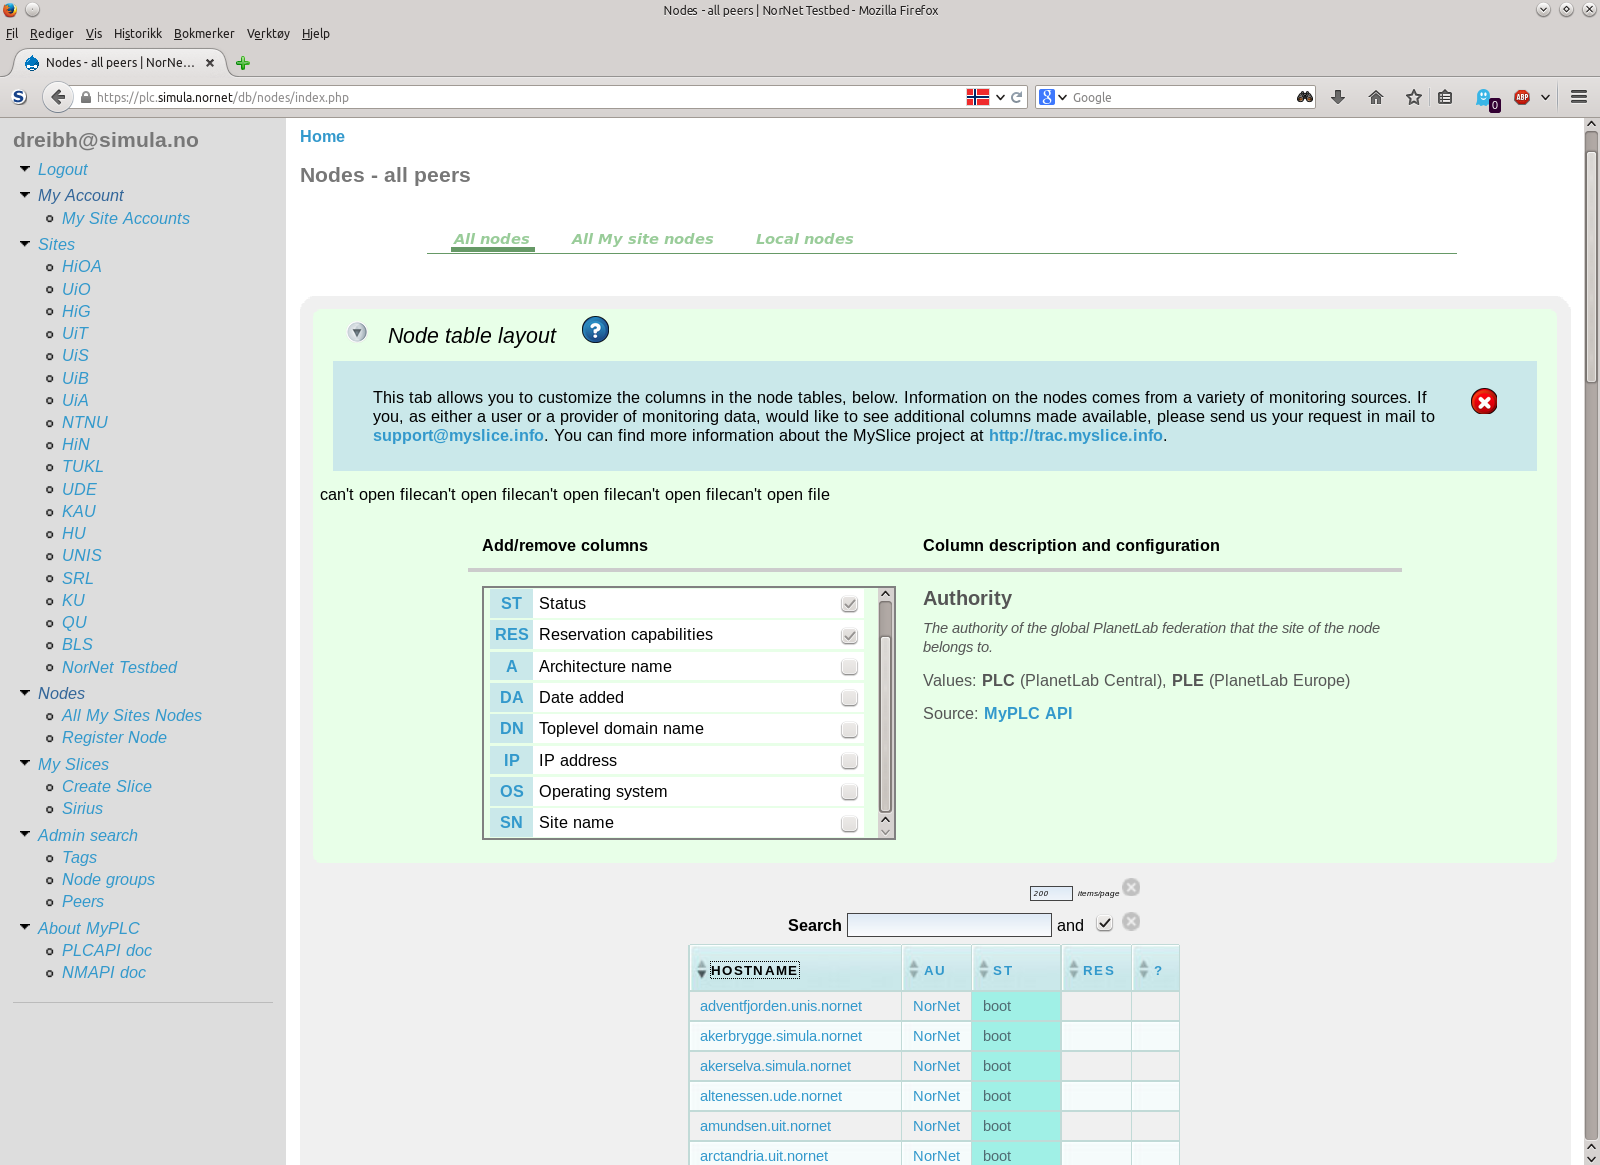
\includegraphics[width=0.95\columnwidth]{%
   Images/PDF/Screenshot-PLC-Nodes.pdf}
\end{center}
\caption{Nodes}
\label{cap:PLC-Nodes}
\end{figure*}
% %%%%%%%%%%%%%%%%%%%%%%%%%%%%%%%%%%%%%%%%%%%%%%%%%%%%%%%%%

The ``Nodes''\index{Nodes} section, as depicted in Figure~\ref{cap:PLC-Nodes}, presents a list of all research nodes in the testbed. The search field allows for filtering, e.g.\ by entering parts of the DNS names. That is, using e.g.\ ``.uia.nornet'' will filter for all nodes at the .uia.nornet site at \foreignlanguage{norsk}{Universitetet i Agder\index{Universitetet i Agder}~(UiA)}.

Particularly important is the ``Status'' column of the nodes table. It displays the status of each research node, according to its communication with the PLC. The following status values are important:
\begin{itemize}
 \item ``boot''\index{boot}\index{Boot State!boot}: The node is booted and should be up and running. This is, hopefully, the status of all nodes in the list.
 \item ``failboot''\index{failboot}\index{Boot State!failboot}: Booting has failed for some reason. The node is not usable and the \noun{NorNet Core} staff should check the node's status.
 \item ``reinstall''\index{reinstall}\index{Boot State!reinstall}: The node is most likely unusable. When it boots the next time, it will perform a complete reinstall. This is also the status of newly added nodes.
\end{itemize}


% %%%%%%%%%%%%%%%%%%%%%%%%%%%%%%%%%%%%%%%%%%%%%%%%%%%%%%%%%
\begin{figure*}
\begin{center}
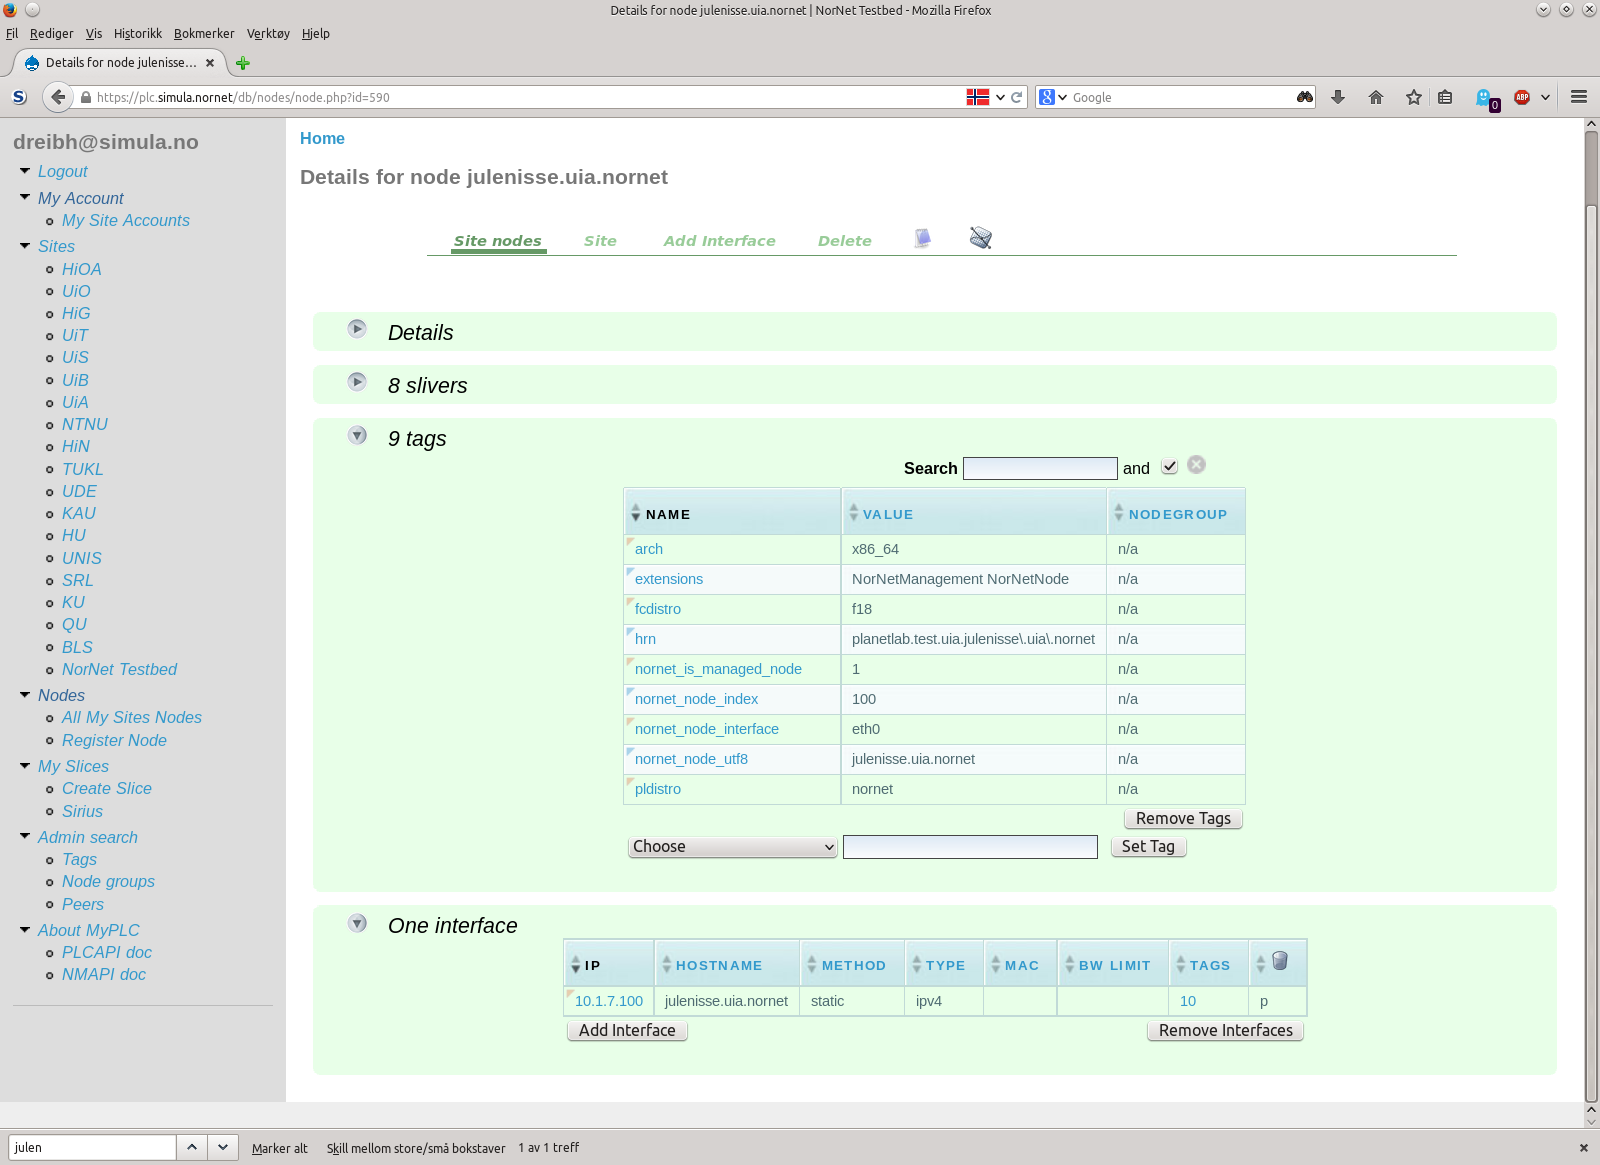
\includegraphics[width=0.95\columnwidth]{%
   Images/PDF/Screenshot-PLC-Node-julenisse.pdf}
\end{center}
\caption{Nodes $\rightarrow$ Node julenisse.uia.nornet}
\label{cap:PLC-Node-Details}
\end{figure*}
% %%%%%%%%%%%%%%%%%%%%%%%%%%%%%%%%%%%%%%%%%%%%%%%%%%%%%%%%%

Clicking on a research node displays details about the node itself, as shown in Figure~\ref{cap:PLC-Node-Details} for the node julenisse.uia.nornet\index{julenisse.uia.nornet}. \noun{NorNet Core}-specific configuration settings are stored in custom tags in the PLC database, together with some ``standard'' PLC tags. Some important tags to be noted here are:
\begin{itemize}
 \item ``arch''\index{arch}\index{Tag!arch}: The architecture of the system. It is currently always x86\_64 (i386 or other CPU types are not supported).

 \item ``fcdistro''\index{fcdistro}\index{Tag!fcdistro}: The variant of \noun{Fedora Core Linux} that runs on the node, e.g.\ ``fc18'' for version~18.

 \item ``pldistro''\index{pldistro}\index{Tag!pldistro}: The software distribution that is installed on the research nodes. Possible values are currently ``lxc'' (stock \noun{PlanetLab}-LXC software) and ``nornet'' (the \noun{NorNet} distribution).
 % , to be introduced in Chapter~\ref{cha:Distribution}).
 
 \item ``nornet\_is\_managed\_node''\index{nornet\_is\_managed\_node}\index{Tag!nornet\_is\_managed\_node}: Denotes whether the research node is a \noun{NorNet Core}-managed node~(``1'') or not~(``0''). \noun{NorNet Core}-managed nodes are assumed to be modified by scripts on the PLC server (by the \noun{NorNet Core} staff) only. Therefore, the configuration of the nodes should \emph{not} be changed in the PLC web interface (even if the user's role allows to do this) to avoid misconfiguration!

 \item ``nornet\_node\_utf8''\index{nornet\_node\_utf8}\index{Tag!nornet\_node\_utf8}: The node name in UTF-8 representation. All node names must use ASCII names in the PLC configuration. However, this tag allows to use special characters (like ``vækerø.simula.nornet''\index{vækerø.simula.nornet}); the DNS configuration can then generate appropriate Internationalised Domain Names\index{Internationalised Domain Names}\nomenclature{IDN}{Internationalised Domain Name}~(IDN\index{IDN|see{Internationalised Domain Names}}, \cite{RFC3492}) references to the ASCII version (e.g.\ ``vækerø.simula.nornet'' $\rightarrow$ ``vaekeroe.simula.nornet''\index{vaekeroe.simula.nornet}) as well.
 
 \item ``nornet\_node\_index''\index{nornet\_node\_index}\index{Tag!nornet\_node\_index}: The node index of the node (root context).
 
 \item ``nornet\_node\_interface''\index{nornet\_node\_interface}\index{Tag!nornet\_node\_interface}: The name of the \noun{NorNet Core} network interface (usually: ``eth0'').
 
 \item ``nornet\_node\_machine\_host''\index{nornet\_node\_machine\_host}:\index{Tag!nornet\_node\_machine\_host} If the research node is a virtual machine, the name of the physical host can be specified here.
 
 \item ``nornet\_node\_machine\_display''\index{nornet\_node\_machine\_display}\index{Tag!nornet\_node\_machine\_display}: If available, a URL to remotely access the display of the node can be specified here.

 \end{itemize}


% %%%%%%%%%%%%%%%%%%%%%%%%%%%%%%%%%%%%%%%%%%%%%%%%%%%%%%%%%
\begin{figure*}
\begin{center}
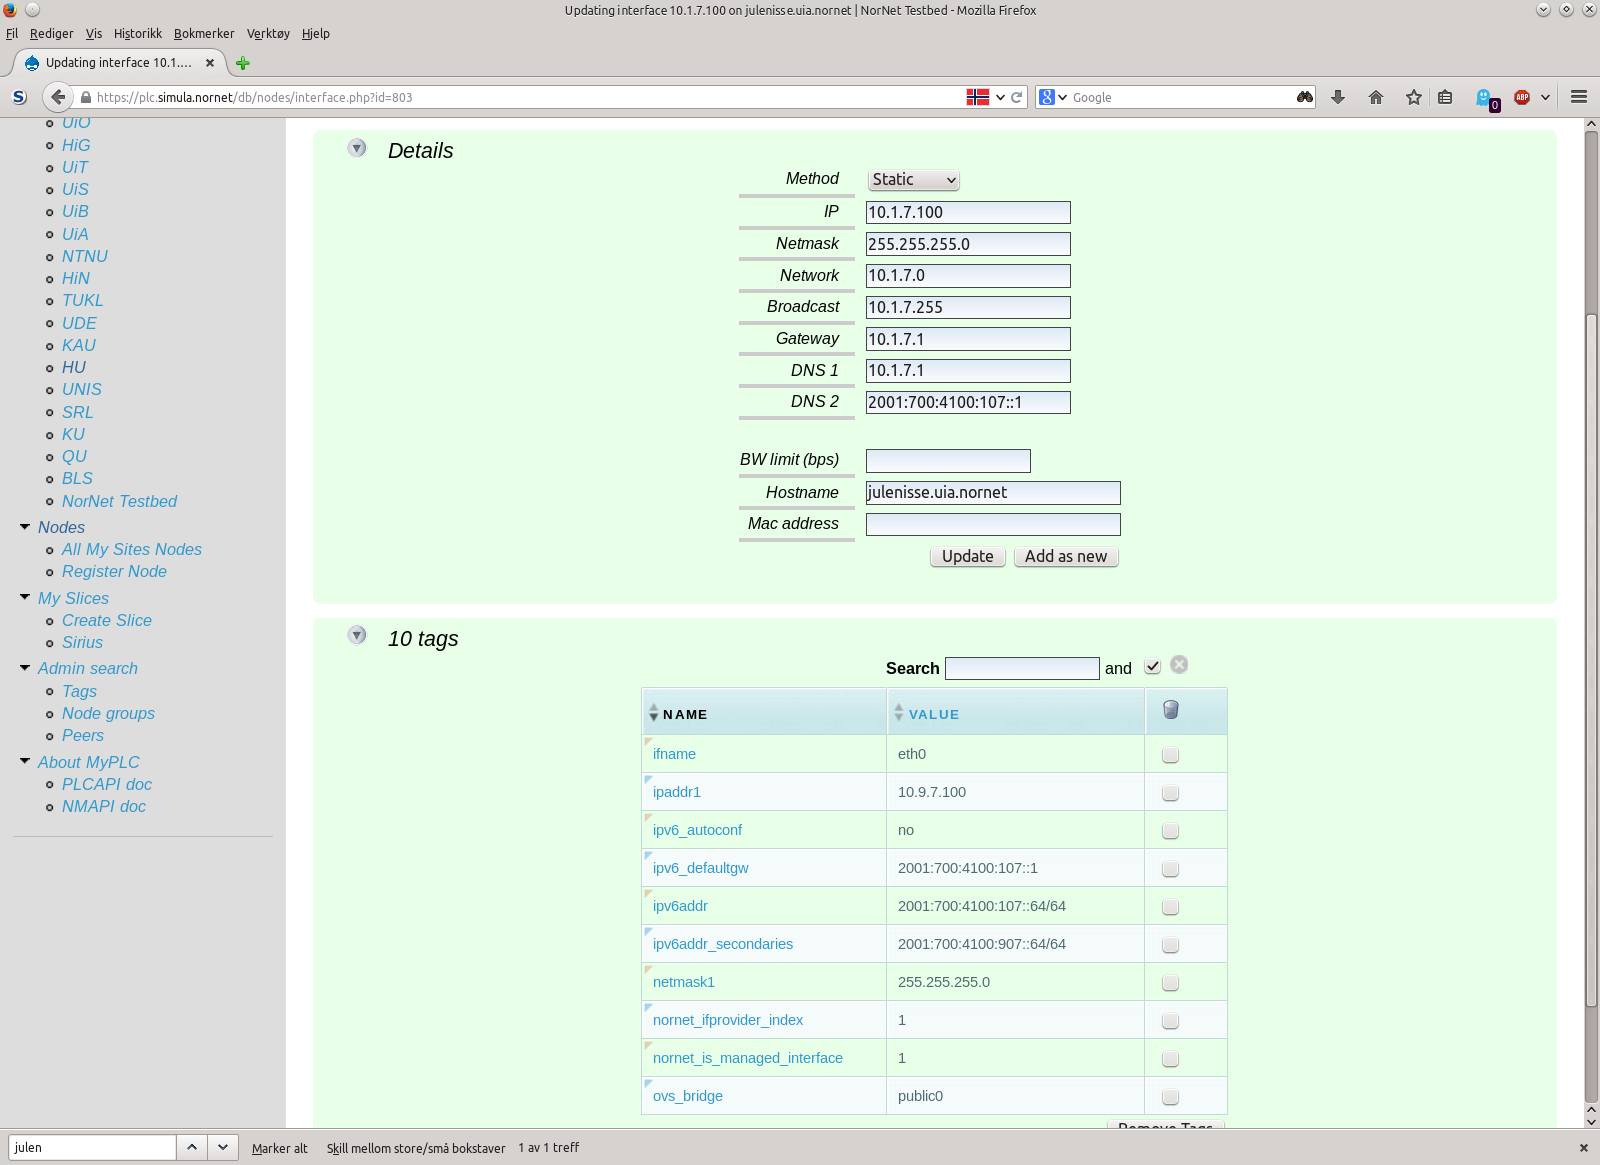
\includegraphics[width=0.95\columnwidth]{%
   Images/PDF/Screenshot-PLC-Node-julenisse-Interface.pdf}
\end{center}
\caption{Nodes $\rightarrow$ Node julenisse.uia.nornet $\rightarrow$ Interface~10.1.7.100}
\label{cap:PLC-Node-Interface-Details}
\end{figure*}
% %%%%%%%%%%%%%%%%%%%%%%%%%%%%%%%%%%%%%%%%%%%%%%%%%%%%%%%%%

The node details page also contains the list of network interfaces. \noun{NorNet Core} nodes usually have only one interface, configured with multiple logical networks (i.e.\ one for each ISP) as well as IPv4 and IPv6. Clicking on this interface will present the interface details, as shown in Figure~\ref{cap:PLC-Node-Interface-Details} for the interface 10.1.10.104 of the research node julenisse.uia.nornet\index{julenisse.uia.nornet}.

The current version of the PLC web interface supports neither multi-homing nor IPv6. Therefore, only the IPv4 configuration of the primary ISP is found directly in this view. IPv6 configuration as well as the configuration for additional ISPs is completely stored in PLC tags:
\begin{itemize}
 \item ``ipaddr$N$''\index{ipaddr$N$}\index{Tag!ipaddr$N$}: The IPv4 adddress of the $N+1$-th ISP. Note, that the IPv4 address of the primary interface is stored directly in the configuration, not in the tags.
 
 \item ``netmask$N$''\index{netmask$N$}\index{Tag!netmask$N$}: The IPv4 network mask of the $N+1$-th ISP.

 \item ``ipv6addr''\index{ipv6addr}\index{Tag!ipv6addr}: The IPv6 network address (i.e.\ address/prefix) of the primary ISP.
  
 \item ``ipv6\_defaultgw''\index{ipv6\_defaultgw}\index{Tag!ipv6\_defaultgw}: The IPv6 default gateway of the primary ISP.

 \item ``ipv6addr\_secondaries''\index{ipv6addr\_secondaries}\index{Tag!ipv6addr\_secondaries}: A space-separated list of all other ISPs IPv6 network addresses (i.e.\ address/prefix).
 
 \item ``ipv6\_autoconf''\index{ipv6\_autoconf}\index{Tag!ipv6\_autoconf}: Enables (``on'') or disables (``off'') IPv6 auto-configuration. It must be turned off for \noun{NorNet Core} interfaces.

 \item ``nornet\_ifprovider\_index''\index{nornet\_ifprovider\_index}\index{Tag!nornet\_ifprovider\_index}: The provider index (see Chapter~\ref{cha:Providers}) of the primary ISP.

 \item ``nornet\_is\_managed\_interface''\index{nornet\_is\_managed\_interface}\index{Tag!nornet\_is\_managed\_interface}: Denotes whether the interface is a \noun{NorNet Core}-managed interface~(``1'') or not~(``0''). \noun{NorNet Core}-managed interfaces are assumed to be modified by scripts on the PLC server (by the \noun{NorNet Core} staff) only. Therefore, the configuration of the interfaces should \emph{not} be changed in the PLC web interface (even if the user's role allows to do this) to avoid misconfiguration!

 \item ``ovs\_bridge''\index{ovs\_bridge}\index{Tag!ovs\_bridge}: This is the research nodes's network interface, as provided by \noun{Open vSwitch}\index{Open vSwitch}. It should be ``public0''.

 \item ``ifname''\index{ifname}\index{Tag!ifname}: This is the physical interface that will be managed by \noun{Open vSwitch}\index{Open vSwitch}. It should be ``eth0''.
\end{itemize}

Details on the research nodes, i.e.\ particularly their IP~addresses for all ISPs, can be found in Chapter~\ref{cha:Site-Details}.


% ===========================================================================
\subsection{Slices and Slivers}
\label{sub:Slices-and-Slivers}
% ===========================================================================

% %%%%%%%%%%%%%%%%%%%%%%%%%%%%%%%%%%%%%%%%%%%%%%%%%%%%%%%%%
\begin{figure*}
\begin{center}
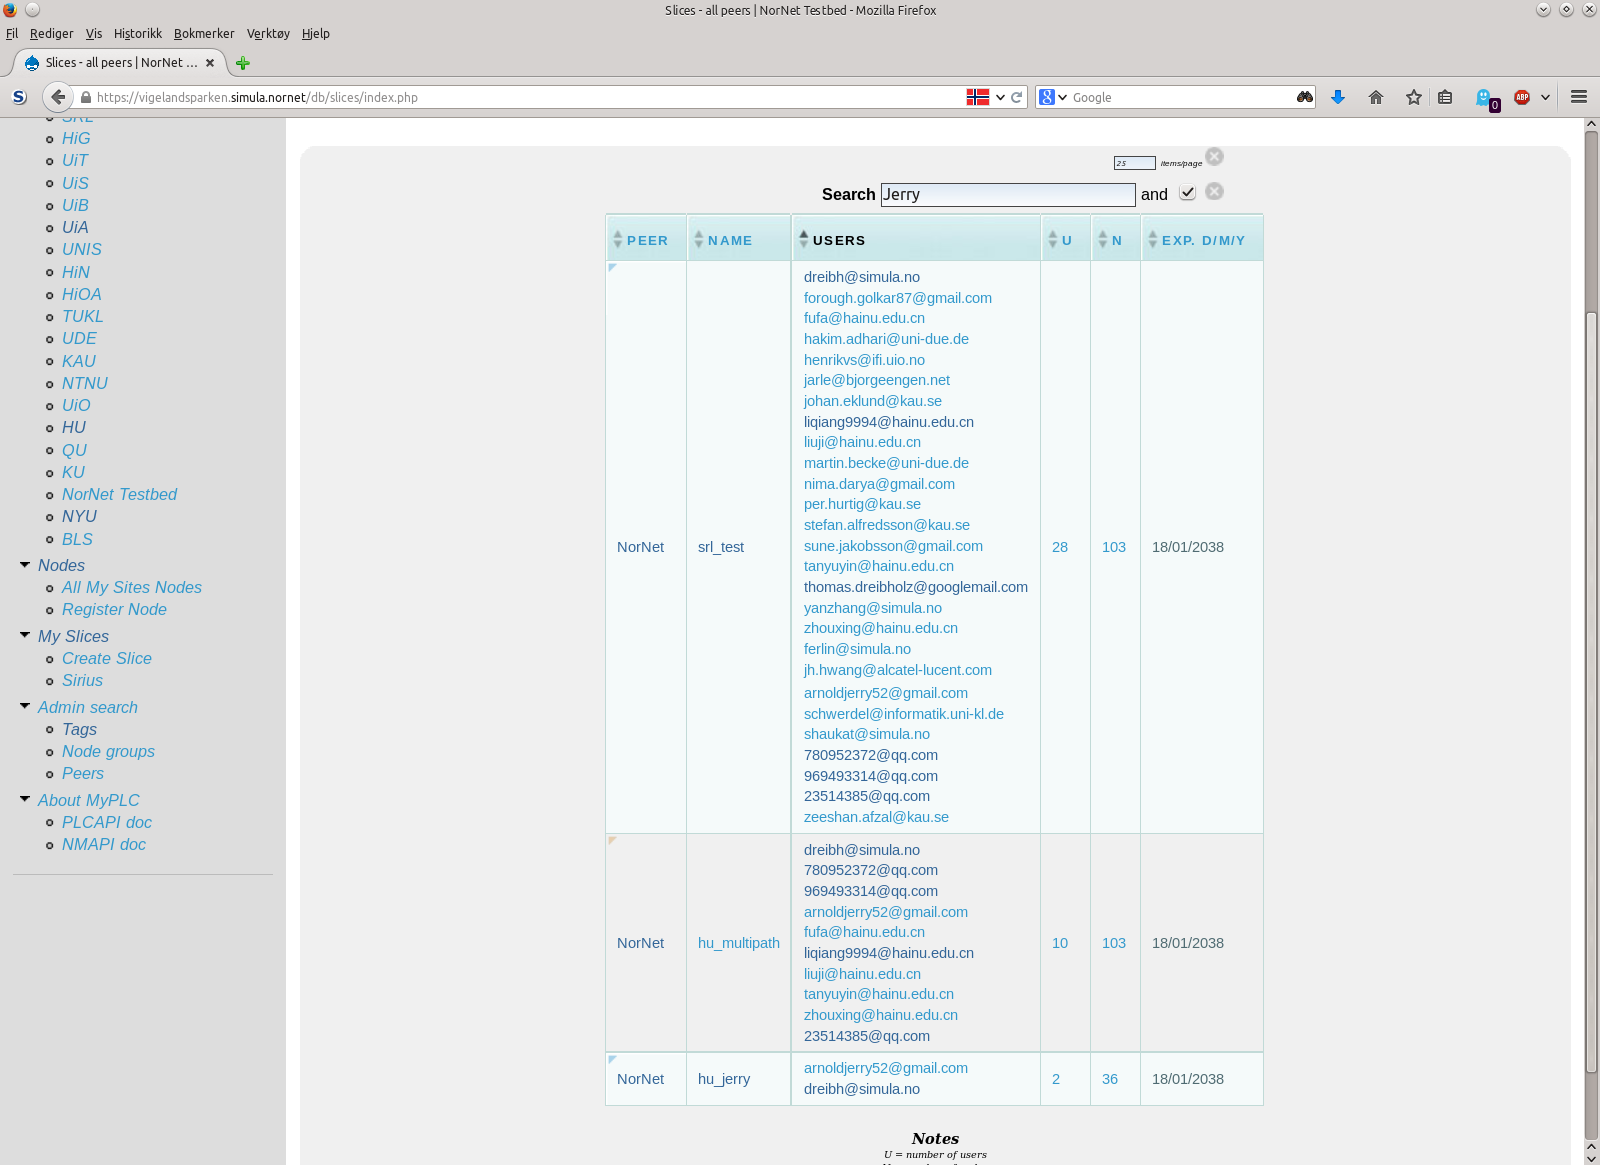
\includegraphics[width=0.95\columnwidth]{%
   Images/PDF/Screenshot-PLC-Slices.pdf}
\end{center}
\caption{The List of All Slices}
\label{cap:PLC-Slices}
\end{figure*}
% %%%%%%%%%%%%%%%%%%%%%%%%%%%%%%%%%%%%%%%%%%%%%%%%%%%%%%%%%

% %%%%%%%%%%%%%%%%%%%%%%%%%%%%%%%%%%%%%%%%%%%%%%%%%%%%%%%%%
\begin{figure*}
\begin{center}
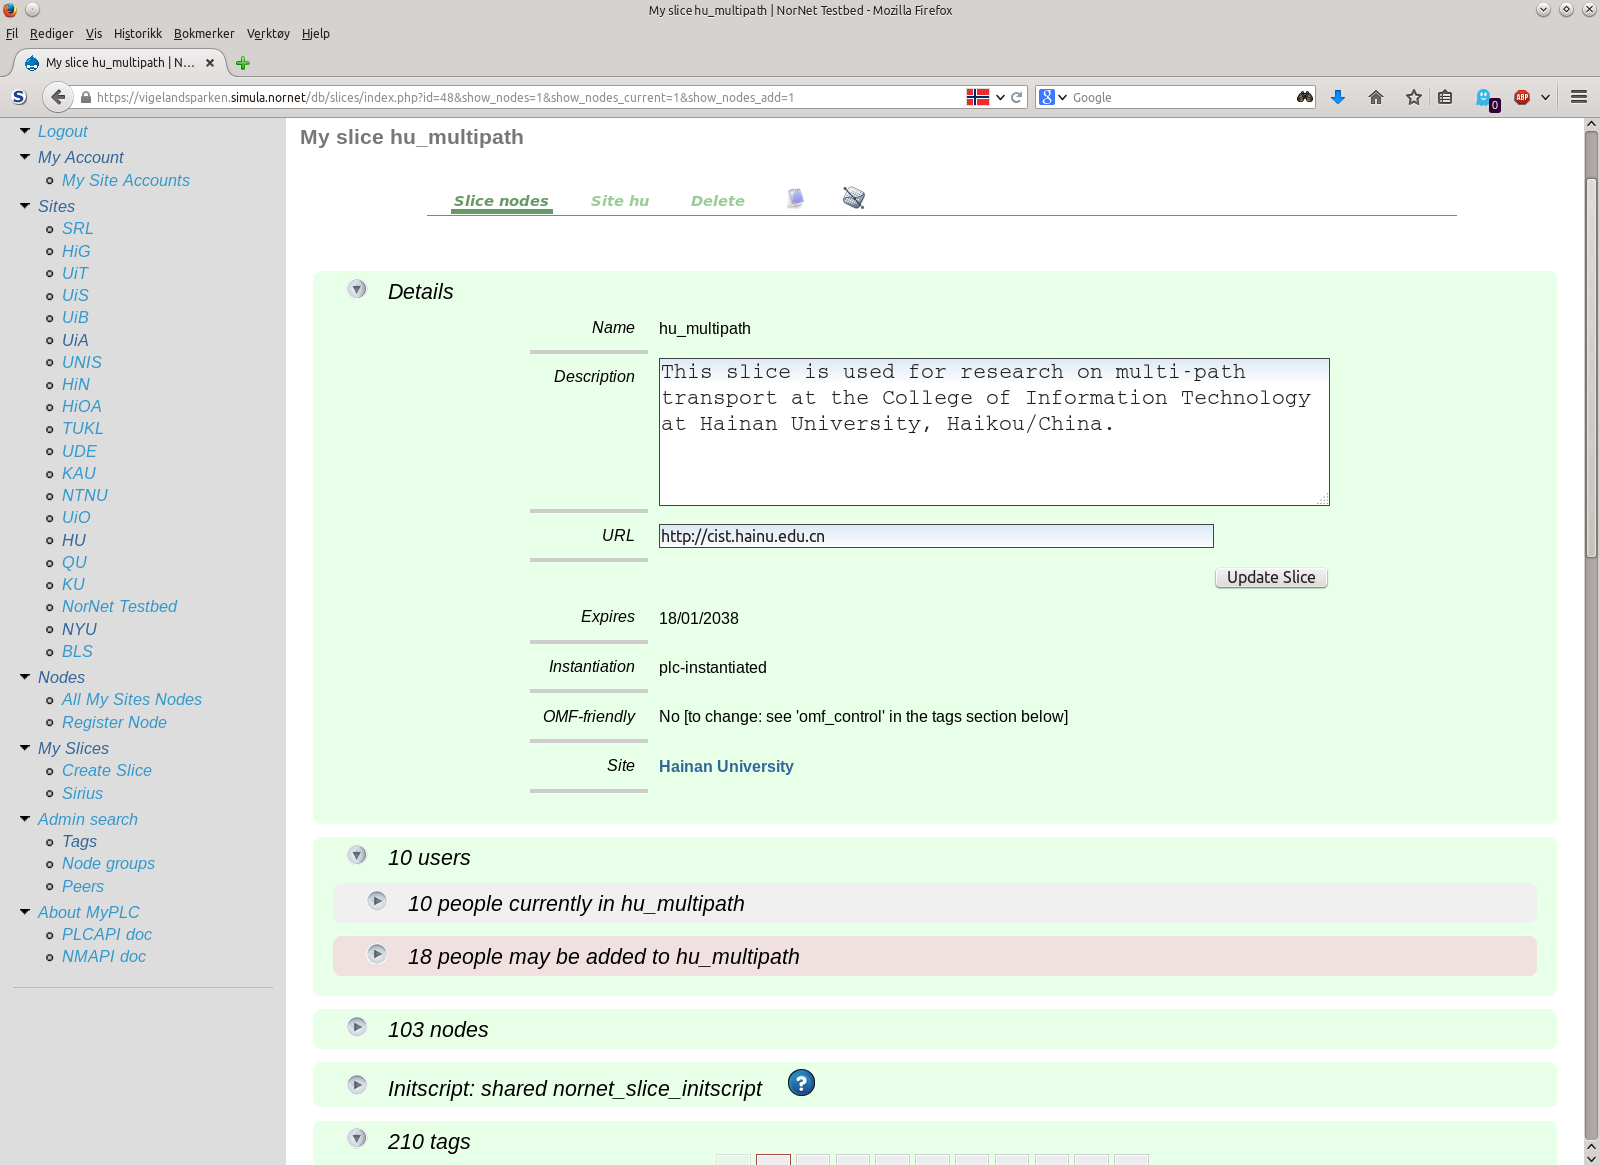
\includegraphics[width=0.95\columnwidth]{%
   Images/PDF/Screenshot-PLC-Slice-hu-multipath.pdf}
\end{center}
\caption{My Slices $\rightarrow$ hu\_multipath}
\label{cap:PLC-Slice-hu-multipath}
\end{figure*}
% %%%%%%%%%%%%%%%%%%%%%%%%%%%%%%%%%%%%%%%%%%%%%%%%%%%%%%%%%


The slices associated with a user are listed under ``My Slices'', as shown in Figure~\ref{cap:PLC-Slices}. Note that the list contains \emph{all} slices in \noun{NorNet Core}, not just the slices of the user himself! It is possible to use the search field to filter for a certain user's slices. Details about a slice can be obtained by clicking on the slice. This will open the slice details view.

An example for the slice details can be found in Figure~\ref{cap:PLC-Slice-hu-multipath} for the slice ``hu\_multipath''. Particularly, for the users associated with a slice, it allows to edit the slice description as well as a public URL. The users of \noun{NorNet Core} slices are \emph{required} to keep their slice descriptions and URLs up-to-date, in order to inform people about what is going on in their slice! It will also help debugging problems when something goes wrong or causes unusual behaviour.

The slice details page also allows to add/remove nodes from/to the slice.
\\
\textbf{Adding nodes does not work at the moment! Ask \noun{NorNet Core} staff to do this via script. Otherwise, the slivers will get no IP~configuration!}

\noun{NorNet}-specific slice information is stored in the following PLC tags:
\begin{itemize}
 \item ``nornet\_is\_managed\_slice''\index{nornet\_is\_managed\_slice}\index{Tag!nornet\_is\_managed\_slice}: Denotes whether the research slice is a \noun{NorNet Core}-managed slice~(``1'') or not~(``0''). \noun{NorNet Core}-managed slices are assumed to be modified by scripts on the PLC server (by the \noun{NorNet Core} staff) only. Therefore, the configuration of the slices should \emph{not} be changed in the PLC web interface (even if the user's role allows to do this) to avoid misconfiguration!

 \item ``nornet\_slice\_own\_addresses''\index{nornet\_slice\_own\_addresses}\index{Tag!nornet\_slice\_own\_addresses}: If set to ``1'', the sliver gets its own IP~addresses. This is the normal behaviour for \noun{NorNet Core} slivers that intend to use multi-homing. With ``0'', the behaviour is like for \noun{PlanetLab}, i.e.\ addresses are shared among slivers.

 \item ``nornet\_slice\_node\_index''\index{nornet\_slice\_node\_index}\index{Tag!nornet\_slice\_node\_index}: This tag is a node-specific tag. That is, for each node associated with the slice, there may be a separate nornet\_slice\_node\_index tag. The tag defines the node index of the sliver. It is then used to systematically allocate the IP~addresses in case of using own IP~addresses for the sliver.
 
 \item ``interface''\index{interface}\index{Tag!interface}: This node-specific tag contains the contents of a \noun{Fedora Core Linux} network interface configuration file (i.e.\ \texttt{/etc/sysconfig/network-scripts/ifcfg-eth0}\index{ifcfg-eth0}), as string representation of a Python dictionary. This tag is generated by the management script on the PLC, according to a site's ISP configuration and the value of the nornet\_slice\_node\_index tag. It is used by the Node Manager
 % (to be introduced in Section~\ref{sec:Node-Manager})
 to generate the corresponding network configuration for the sliver.
\end{itemize}

Details on the research nodes, i.e.\ particularly their slivers and all IP~addresses, can be found in Chapter~\ref{cha:Site-Details}.



% ###########################################################################
\section{``Kontrollsenteret'' -- The Control Center}
\label{sec:Kontrollsenteret}
% ###########################################################################

% %%%%%%%%%%%%%%%%%%%%%%%%%%%%%%%%%%%%%%%%%%%%%%%%%%%%%%%%%
\begin{figure*}
\begin{center}
\subfigure[Weather Overlays\label{subcap:Kontrollsenteret-Overlays}]{%
   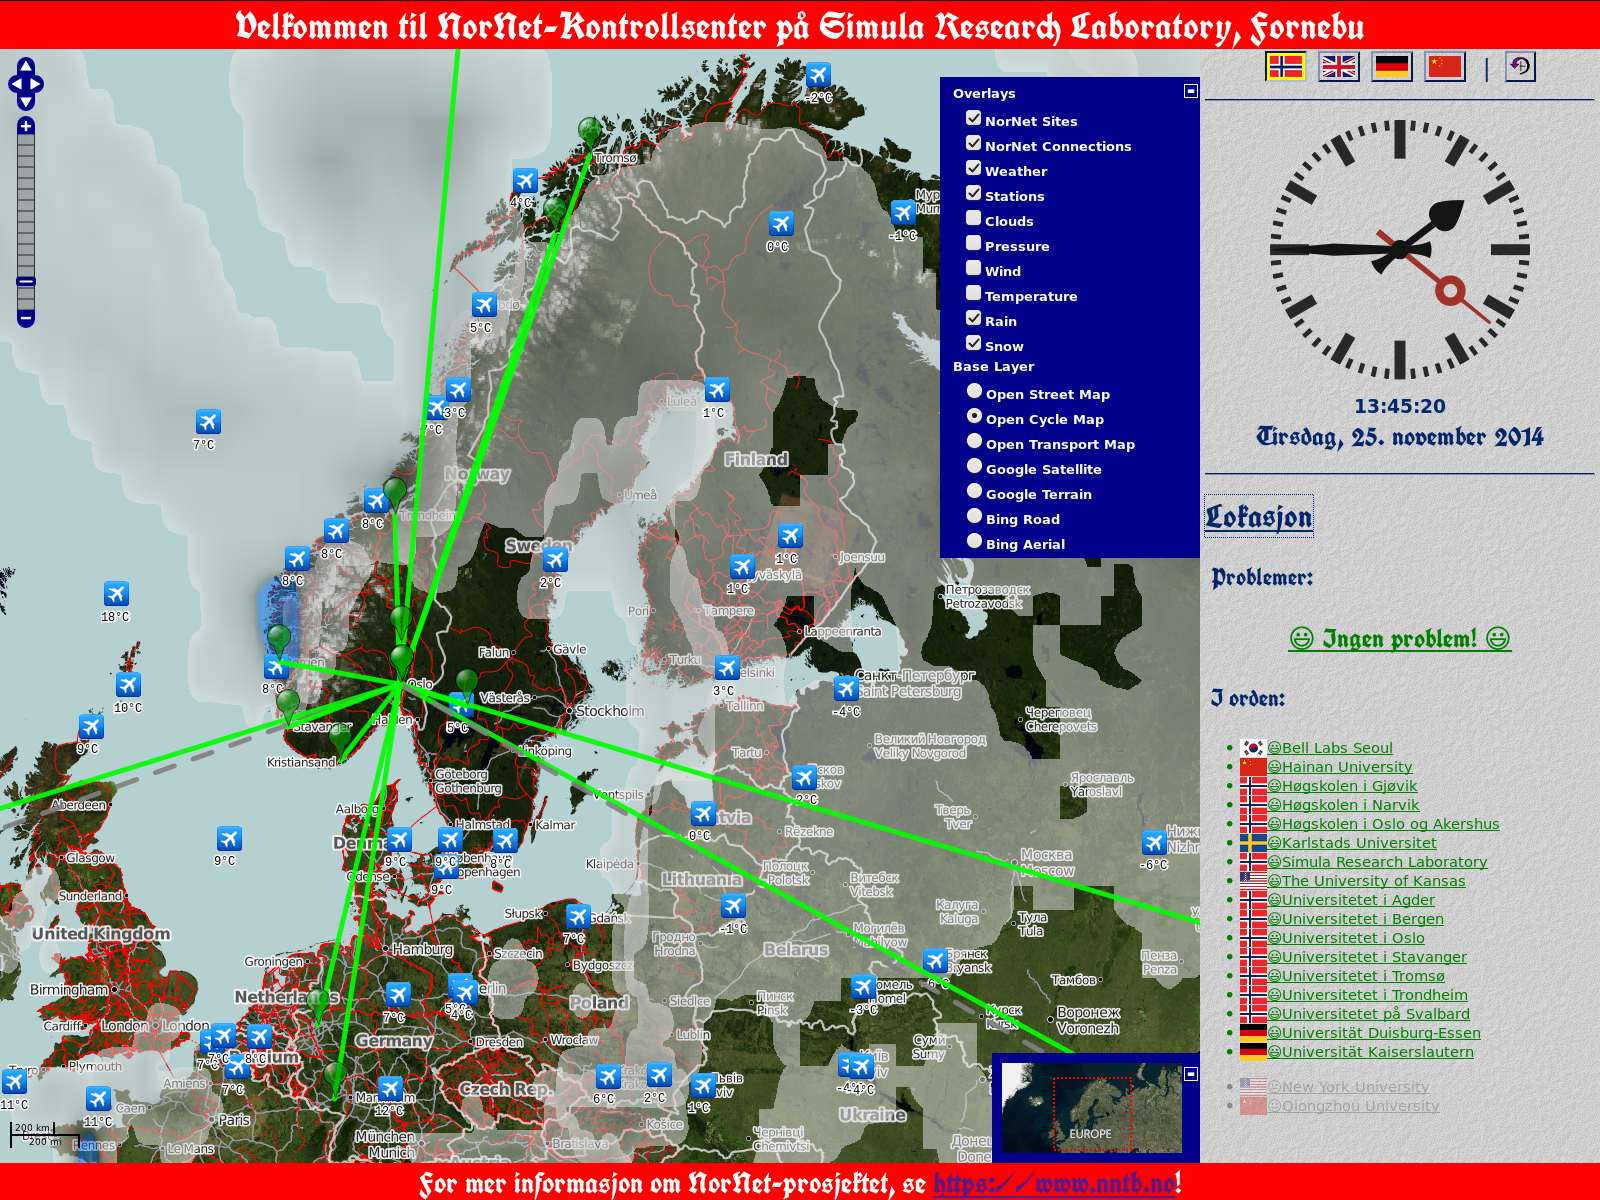
\includegraphics[width=0.825\columnwidth]{Images/PDF/Kontrollsenteret-25Nov2014.pdf}}
\subfigure[Site Information View\label{subcap:Kontrollsenteret-Site}]{%
   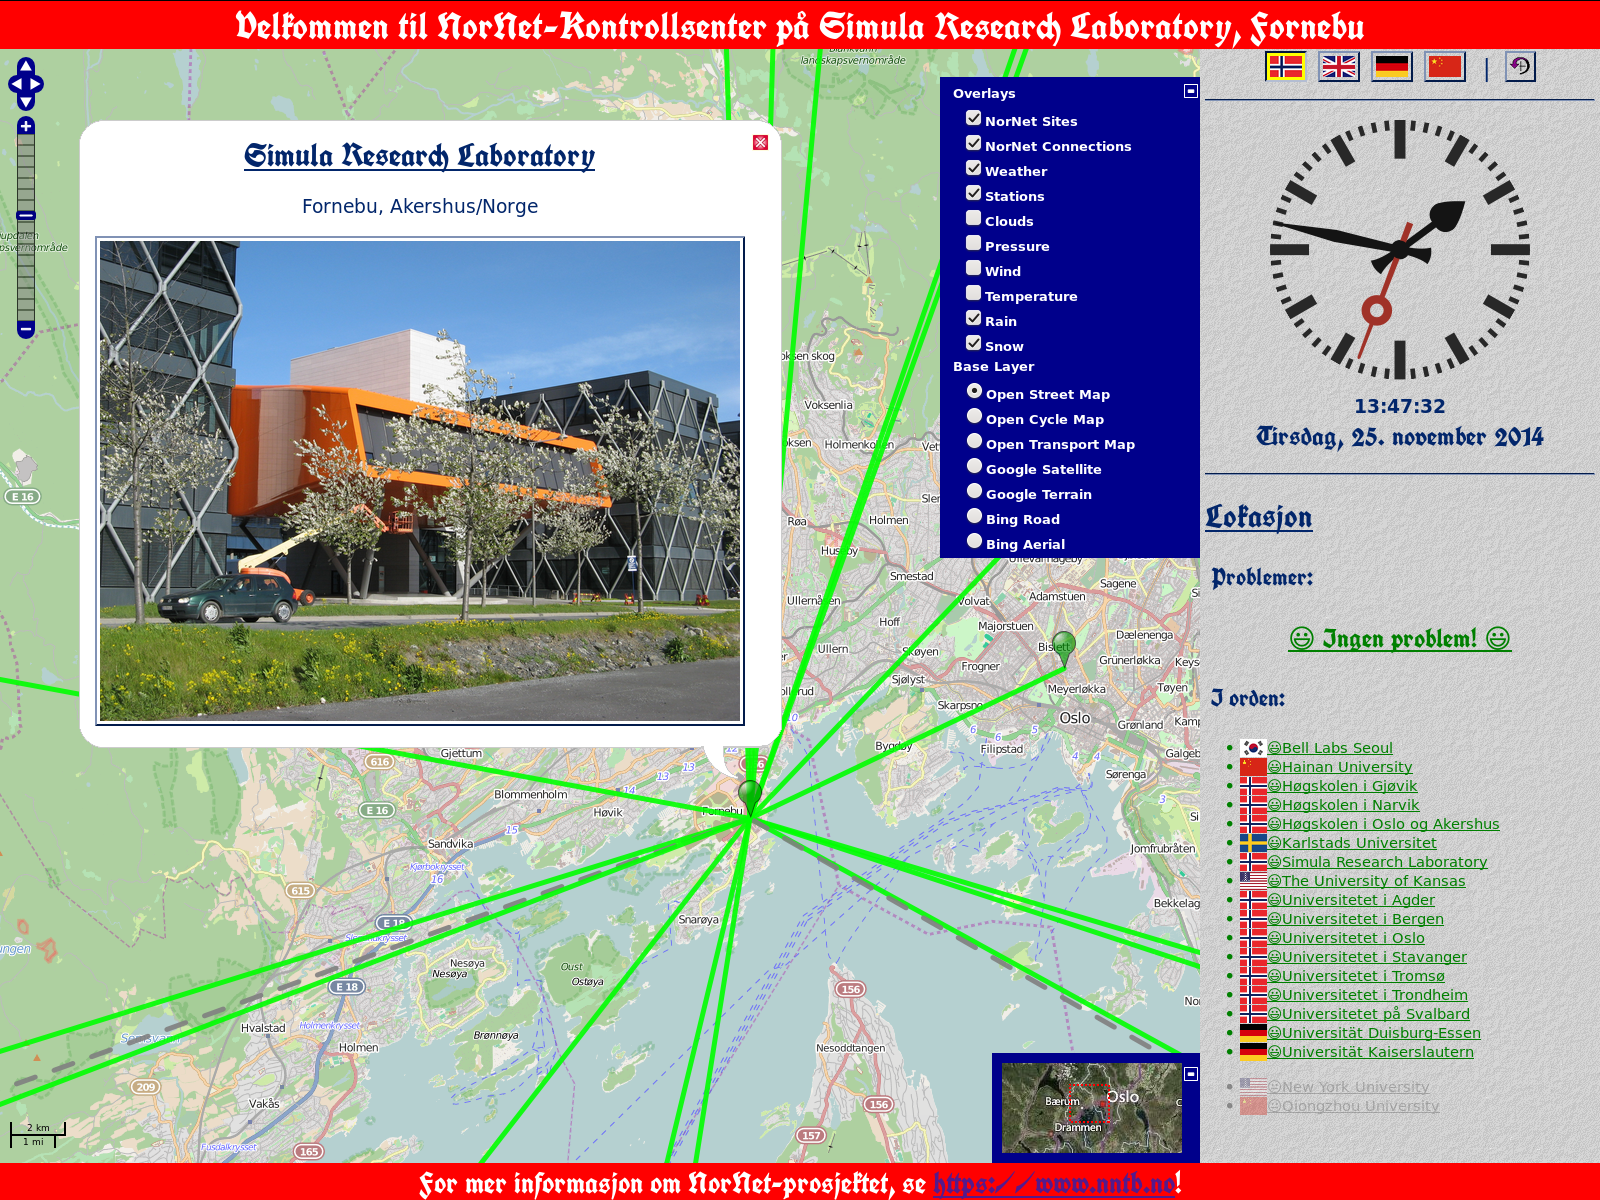
\includegraphics[width=0.825\columnwidth]{Images/PDF/Kontrollsenteret-Simula-25Nov2014.pdf}}
\end{center}
\caption{\noun{NorNet-Kontrollsenter} with Open Street Map Base Layer}
\label{cap:Kontrollsenteret-Site-Information}
\end{figure*}
% %%%%%%%%%%%%%%%%%%%%%%%%%%%%%%%%%%%%%%%%%%%%%%%%%%%%%%%%%

In order to get a quick overview over the status of the sites and tunnels (i.e.\ the reachability and routing among the tunnelboxes), the \noun{NorNet-Kontrollsenter}\index{Kontrollsenteret}\index{NorNet-Kontrollsenter} service on the Monitor server can be used via web browser. There are two possibilities to connect to this service:
\begin{itemize}
 \item \url{http://monitor.simula.nornet}:
 In case of connection to the local \noun{NorNet Core} network including its DNS service, the web browser can directly connect to the Monitor server.
 
 \item \url{http://localhost:2001}:
 If access to the \noun{NorNet Core} network is only available via the Gatekeeper server, the SSH port forwarding -- as described in Subsubsection~\ref{subsub:Tunnelling-TCP-Connections} -- can be used. Then, if using the settings described there, the web browser connects to the local machine's port~2001. This port is forwarded, via SSH and the Gatekeeper server, to the Monitor server.
\end{itemize}

The \noun{NorNet-Kontrollsenter} displays the \noun{NorNet Core} sites on a map view, as described in Subsection~\ref{sub:The-Monitoring-Setup}, with the \noun{OpenLayers}~\cite{OpenLayersDoc} JavaScript library utilising map services in the Internet, currently \noun{Open Street Map}\footnote{\noun{Open Street Map}: \url{http://www.openstreetmap.org/}.}, \noun{Google Maps} and \noun{Bing Maps}\footnote{\noun{Bing Maps}: \url{http://www.bing.com/maps/}.}. Note, that due to access restrictions in some countries, some of the used map services may not be accessible (e.g.\ \noun{Google Maps} in China). Also, the JavaScript handling of map data is computation-intensive and requires a web browser with up-to-date features. \noun{NorNet-Kontrollsenter} is mainly tested and known to work with \noun{Firefox}.

An example screenshot of the \noun{NorNet-Kontrollsenter} is shown in Figure~\ref{cap:Kontrollsenteret-Site-Information}: Subfigure~\ref{subcap:Kontrollsenteret-Overlays} presents a view on the European \noun{NorNet Core} sites, using an \noun{Open Street Map} base layer and some weather information overlays.

The status of sites is displayed by site marker colours as follows:
\begin{itemize}
 \item green: The tunnelbox is reachable via all tunnels over all ISP combinations and all available IP~protocols (i.e.\ IPv4 and IPv6).
 \item orange: Some of the the endpoint addresses of the tunnelbox are not reachable, but at least some addresses are reachable.
 \item red: No address of the tunnelbox is reachable.
 \item black: The site is set as inactive in the PLC configuration (e.g.\ a new site that is not yet fully installed).
\end{itemize}
Lines among the sites denote the status of tunnels:
\begin{itemize}
 \item green: A green line between a remote site and the Central Site at the Simula Research Laboratory denotes a fully-operational site. That is, all tunnels between the site and other sites are working properly. In order to simplify this ``normal'' case, the visualisation is therefore reduced to a single, green line.
 
 \item red: A red line between two sites denotes a not-working tunnel between the corresponding sites.
 
 \item grey: A dotted grey line between a site and the Central Site at the Simula Research Laboratory denotes the connection to an inactive site. For an inactive site, only a tunnel between the site's tunnelbox and the Central Site is configured for testing purposes.
\end{itemize}

Another feature of the \noun{NorNet-Kontrollsenter} is to provide information about sites by clicking on their markers. An example is provided in Subfigure~\ref{subcap:Kontrollsenteret-Site}. Currently, it only displays the site's location and an image of the site.



% ###########################################################################
\section{The Performance Monitor}
\label{sec:PerfMon}
% ###########################################################################

% %%%%%%%%%%%%%%%%%%%%%%%%%%%%%%%%%%%%%%%%%%%%%%%%%%%%%%%%%
\begin{figure*}
\begin{center}
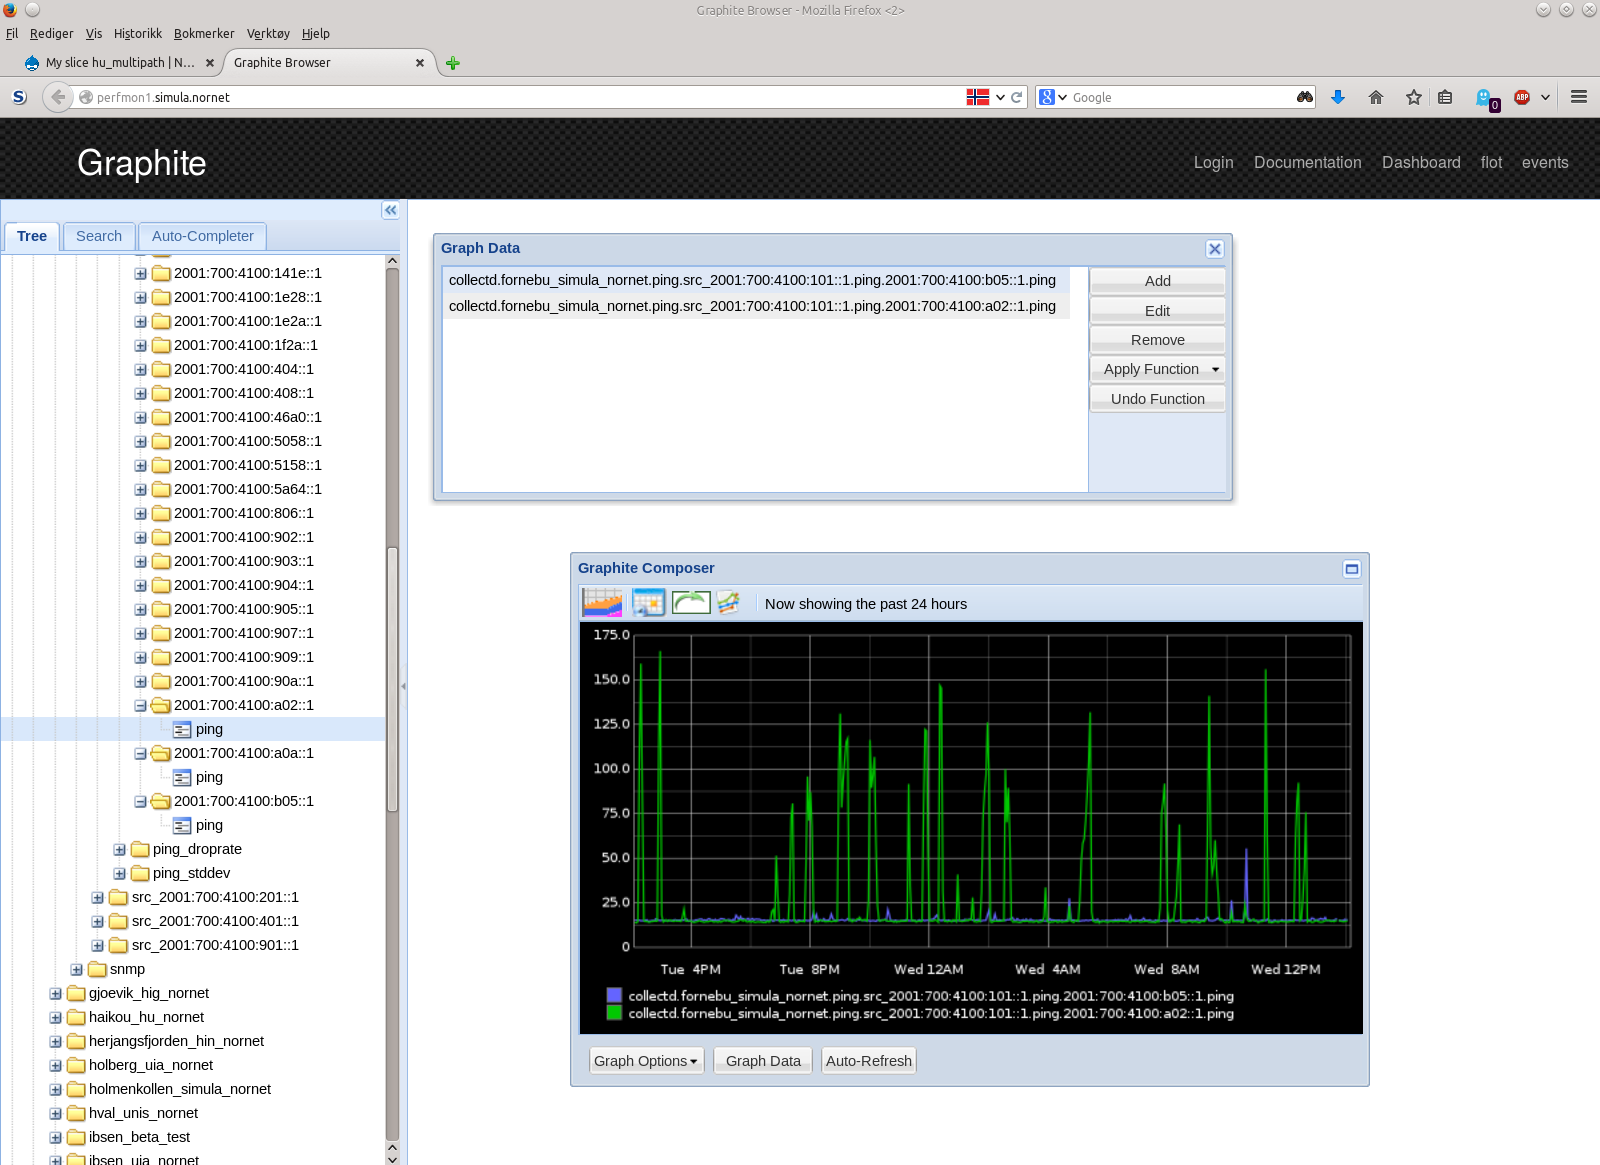
\includegraphics[width=0.95\columnwidth]{%
   Images/PDF/Screenshot-PerfMon1.pdf}
\end{center}
\caption{Performance Visualisation with the Performance Monitor}
\label{cap:PerfMon1}
\end{figure*}
% %%%%%%%%%%%%%%%%%%%%%%%%%%%%%%%%%%%%%%%%%%%%%%%%%%%%%%%%%

In order to get detailed performance data of tunnelboxes, tunnels and other \noun{NorNet Core} systems, the Performance Monitor service on the Performance server can be used via web browser. There are two possibilities to connect to this service:
\begin{itemize}
 \item \url{http://perfmon1.simula.nornet}:
 In case of connection to the local \noun{NorNet Core} network including its DNS service, the web browser can directly connect to the Monitor server.
 
 \item \url{http://localhost:2002}:
 If access to the \noun{NorNet Core} network is only available via the Gatekeeper server, the SSH port forwarding -- as described in Subsubsection~\ref{subsub:Tunnelling-TCP-Connections} -- can be used. Then, if using the settings described there, the web browser connects to the local machine's port~2002. This port is forwarded, via SSH and the Gatekeeper server, to the Monitor server.
\end{itemize}

Figure~\ref{cap:PerfMon1} presents an example view from the Performance Monitor, visualising some Round-Trip Time\nomenclature{RTT}{Round-Trip Time}\index{Round-Trip Time}~(RTT\index{RTT|see{Round-Trip Time}}) measurements between two tunnelboxes.



% ###########################################################################
\section{Further Resources}
% ###########################################################################

% ===========================================================================
\subsection{Sites Overview}
% ===========================================================================

The complete PLC configuration of the \noun{NorNet Core} testbed can be found as an up-to-date summary at \url{https://www.nntb.no/pub/nornet-configuration/NorNetCore-Sites.html}. This is mainly an automatically-updated online HTML version of the information in Part~\ref{prt:Configuration}. However, for security reasons, the online version does not contain any site contacts, the sliver information as well as IP~addresses.

Note, that the site overview on the web page, as well as in Part~\ref{prt:Configuration}, are automatically exported from the PLC database by using the tool \texttt{Get-NorNet-Configuration}\index{Get-NorNet-Configuration}. It is installed on the Gatekeeper server. A manual page is provided as well\footnote{\texttt{Get-NorNet-Configuration} manual page: \texttt{\href{man:Get-NorNet-Configuration}{man Get-NorNet-Configuration}}.}. The program extracts the PLC database's contents to HTML as well as \LaTeX\index{\LaTeX} output:
\begin{itemize}
 \item HTML: Generating HTML output is as simple as:
\begin{lstlisting}
Get-NorNet-Overview -html >Overview.html
\end{lstlisting}
The resulting HTML page \texttt{Overview.html} can be viewed with any web browser (it is actually valid XHTML\index{XHTML}~1.1~\cite{recommendation-W3C-XHTML1.1} code).

 \item \LaTeX: The \LaTeX{} output of course requires compiling the document to Portable Document Format\nomenclature{PDF}{Portable Document Format}\index{Portable Document Format}~(PDF\index{PDF|see{Portable Document Format}}) for viewing. The complete command sequence is therefore:
\begin{lstlisting}
Get-NorNet-Overview -latex >Overview.tex && \
pdflatex Overview.tex && \
makeindex Overview.nlo -s nomencl.ist -o Overview.nls && \
makeindex Overview.idx && \
pdflatex Overview.tex && \
makeindex Overview.idx && \
pdflatex Overview.tex 
\end{lstlisting}
The output PDF file is then named \texttt{Overview.pdf}.

\end{itemize}



% ===========================================================================
\subsection{Mailing Lists}
% ===========================================================================

There are currently two mailing lists\index{Mailing Lists} for \noun{NorNet}-related postings:

\begin{itemize}
 \item \noun{NorNet}~Announcements\index{Mailing Lists!\noun{NorNet} Announcements}:
 A list with general announcements about \noun{NorNet}, e.g.\ workshops, conferences, etc..
 The registration to this list can be managed at \url{https://sympa.uio.no/ifi.uio.no/modindex/nornet-announcements}.

 \item \noun{NorNet}~Users\index{Mailing Lists!\noun{NorNet} Users}:
 A list with announcements for \noun{NorNet} users, e.g.\ maintenance, changes of the infrastructure, etc.. It is assumed that all \noun{NorNet} users are subscribed to this list.
 The registration to this list can be managed at \url{https://sympa.uio.no/ifi.uio.no/modindex/nornet-users}.
\end{itemize}


% ===========================================================================
\subsection{Web Server}
% ===========================================================================

% %%%%%%%%%%%%%%%%%%%%%%%%%%%%%%%%%%%%%%%%%%%%%%%%%%%%%%%%%
\begin{figure*}
\begin{center}
\subfigure[The News Section\label{subcap:WebServer-News}]{%
   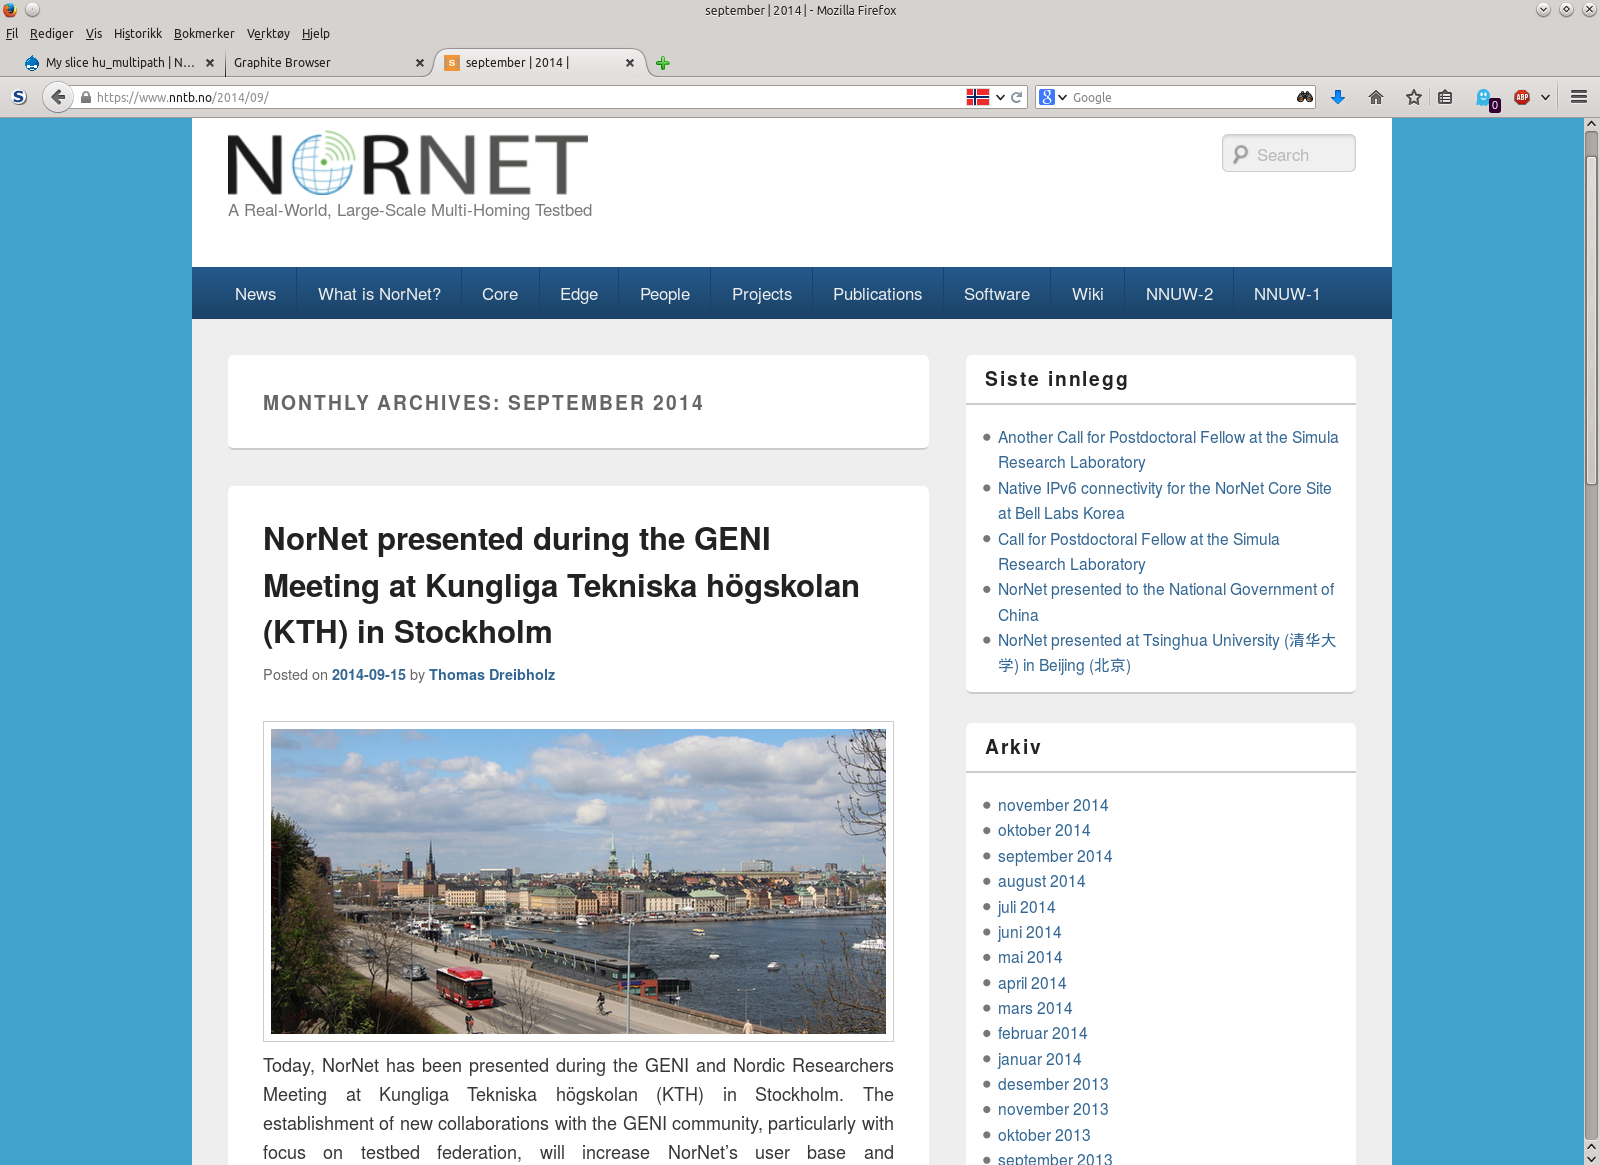
\includegraphics[width=0.825\columnwidth]{Images/PDF/Screenshot-WebServer1.pdf}}
\subfigure[The Publications Section\label{subcap:WebServer-Publications}]{%
   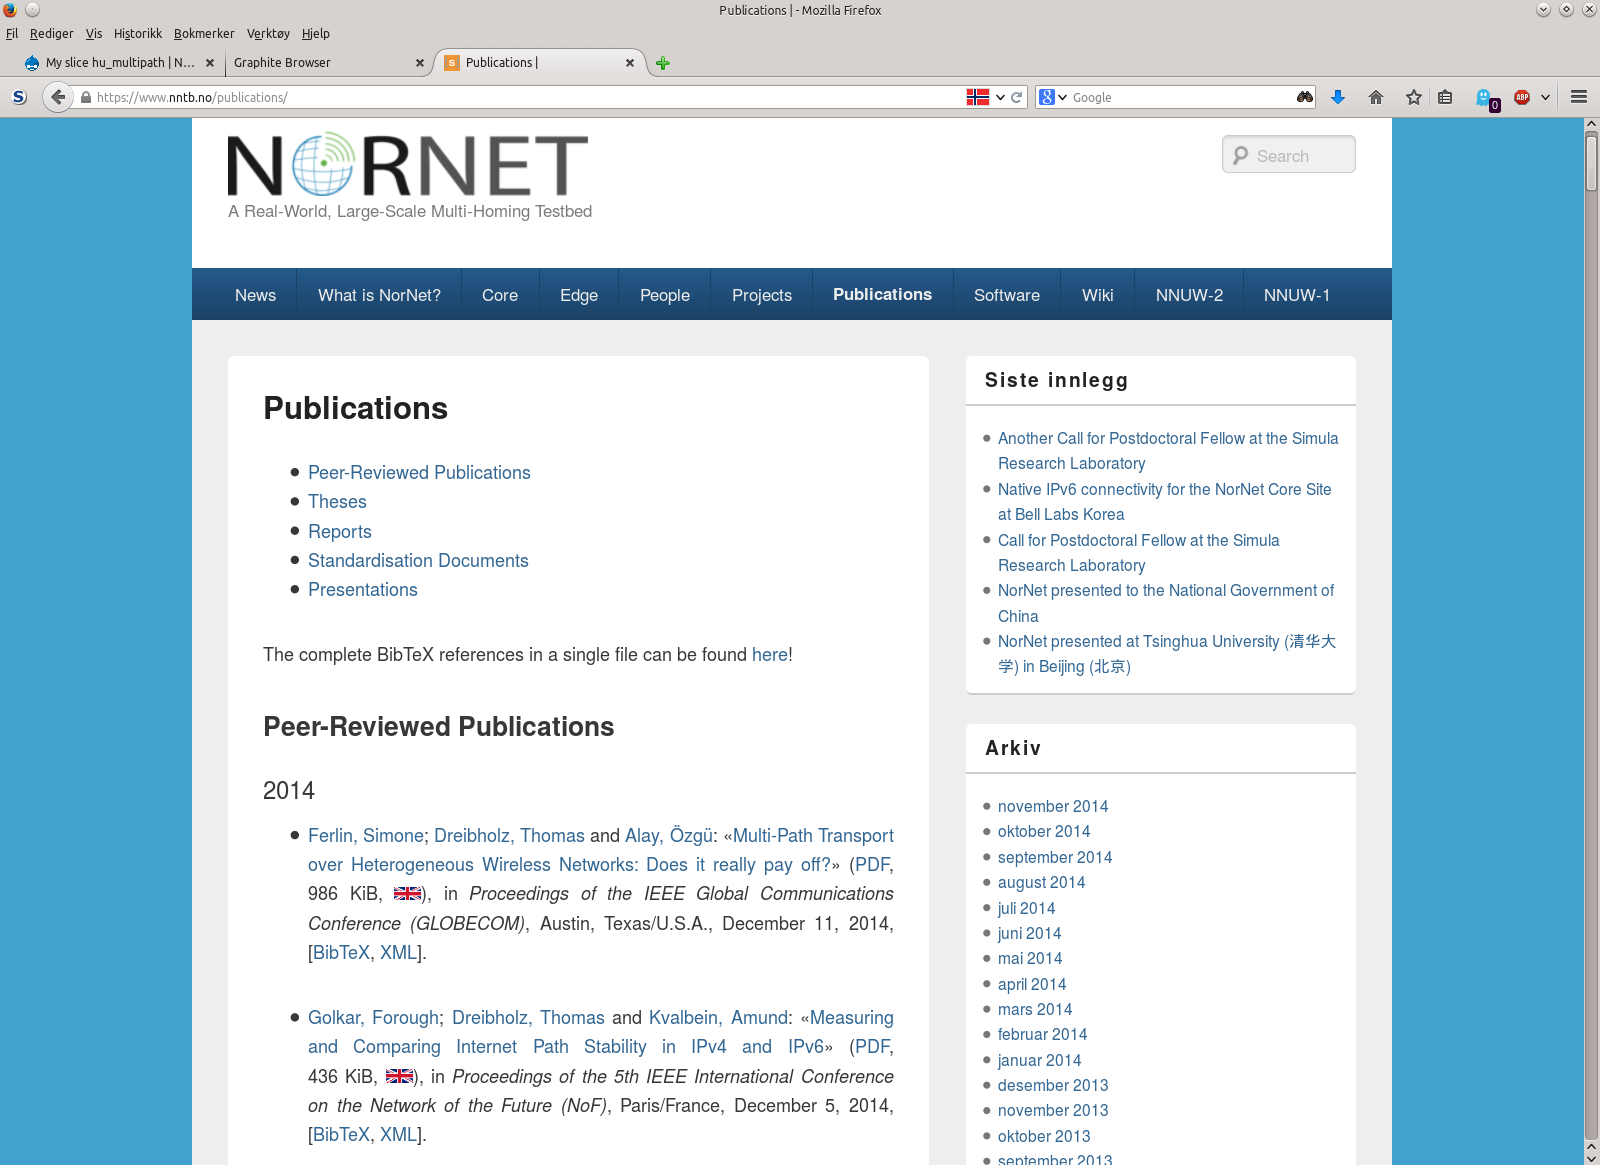
\includegraphics[width=0.825\columnwidth]{Images/PDF/Screenshot-WebServer2.pdf}}
\end{center}
\caption{The \noun{NorNet} Web Server at \url{https://www.nntb.no}}
\label{cap:WebServer}
\end{figure*}
% %%%%%%%%%%%%%%%%%%%%%%%%%%%%%%%%%%%%%%%%%%%%%%%%%%%%%%%%%

The \noun{NorNet} web server\index{Web Server} at \url{https://www.nntb.no}\footnote{\href{https://www.nntb.no}{www.nntb.no}\index{www.nntb.no} is actually an alias for the server \href{http://voksenkollen.simula.nornet}{voksenkollen.simula.nornet}\index{voksenkollen.simula.nornet}.} contains all information about \noun{NorNet Core}. Example views are shown in Figure~\ref{cap:WebServer}. Particularly, it informs about important events such as workshops, new sites and other configuration changes (see Subfigure~\ref{subcap:WebServer-News}).

The web server furthermore contains the complete publications list for \noun{NorNet}, as depicted in (see Subfigure~\ref{subcap:WebServer-Publications}). Particularly, it directly links to most publications and it contains maintained reference data in \BibTeX\index{\BibTeX} and Extensible Markup Language\nomenclature{XML}{Extensible Markup Language}\index{Extensible Markup Language}~(XML\index{XML|see{Extensible Markup Language}}) formats for citing \noun{NorNet}-related documents.
The \noun{NorNet Core} users, of course, are invited to provide references to their own, \noun{NorNet}-related documents for inclusion into the publication list, by sending the corresponding \BibTeX{} information to the \noun{NorNet} staff.


% ===========================================================================
\subsection{Package Server and \noun{Launchpad} PPA}
% ===========================================================================

The Package Server\index{Package Server} at \url{http://packages.nntb.no}\footnote{\href{https://packages.nntb.no}{packages.nntb.no}\index{packages.nntb.no} is actually an alias for the server \href{http://bjoernholt.simula.nornet}{bjoernholt.simula.nornet}\index{bjoernholt.simula.nornet}.} provides some \noun{NorNet}-related software packages for \noun{Fedora Core Linux}\index{Fedora Core}\index{Linux!Fedora Core} as package repositories. In order to use the packages with \texttt{dnf}\footnote{\texttt{dnf} manual page: \texttt{\href{man:dnf}{man dnf}}.}, it is necessary to create a configuration file \texttt{/etc/yum.repos.d/nornet.repo}:
\begin{lstlisting}
[NorNet-Applications]
name=NorNet Applications
baseurl=http://packages.nntb.no/nornet-applications/fedora/$releasever/$basearch
enabled=1
gpgcheck=1
gpgkey=http://www.iem.uni-due.de/~dreibh/key.asc
\end{lstlisting}

For \noun{Ubuntu Linux}\index{Ubuntu}\index{Linux!Ubuntu}, the corresponding packages are \emph{not} hosted on the Package Server. Instead, they are hosted in a Personal Package Archive\nomenclature{PPA}{Personal Package Archive}\index{Personal Package Archive}~(PPA\index{PPA|see{Personal Package Archive}}) on \noun{Launchpad}\index{Launchpad}\footnote{\noun{Launchpad}: \url{https://launchpad.net}.} at \url{https://launchpad.net/~dreibh/+archive/ubuntu/ppa}. The repository can be added to a \noun{Ubuntu} system by using \texttt{apt-add-repository}\footnote{\texttt{apt-add-repository} manual page: \texttt{\href{man:apt-add-repository}{man apt-add-repository}}.}:
\begin{lstlisting}
sudo apt-add-repository ppa:dreibh/ppa
sudo apt-get update
\end{lstlisting}
After that, the packages can be used with \texttt{apt-get}\footnote{\texttt{apt-get} manual page: \texttt{\href{man:apt-get}{man apt-get}}.}.


% ===========================================================================
\subsection{Wiki Server}
% ===========================================================================

There is a \noun{NorNet} wiki\index{Wiki Server} at \url{https://wiki.nntb.no}\footnote{\href{https://wiki.nntb.no}{wiki.nntb.no}\index{wiki.nntb.no} is actually an alias for the server \href{http://tryvannshoegda.simula.nornet}{tryvannshoegda.simula.nornet}\index{tryvannshoegda.simula.nornet}.}. Currently, it is only used internally by the developers. In the future, it is intended to also open this wiki service for \noun{NorNet} users.



% @@@@@@@@@@@@@@@@@@@@@@@@@@@@@@@@@@@@@@@@@@@@@@@@@@@@@@@@@@@@@@@@@@@@@@@@@@@
\chapter{The Research Nodes}
\label{cha:Research-Nodes}
% @@@@@@@@@@@@@@@@@@@@@@@@@@@@@@@@@@@@@@@@@@@@@@@@@@@@@@@@@@@@@@@@@@@@@@@@@@@

...

% ###########################################################################
\section{Logging In}
\label{sec:Logging-In}
% ###########################################################################

...

ssh and keys



% ###########################################################################
\section{Installing Software}
\label{sec:Installing-Software}
% ###########################################################################

dnf ...

gcc, etc.

...


% ###########################################################################
\section{Using Multi-Homing}
\label{sec:Using-Multi-Homing}
% ###########################################################################

ping and traceroute examples

NetPerfMeter!

...


% ###########################################################################
\section{Using Multi-Path TCP}
\label{sec:Using-Multi-Path-TCP}
% ###########################################################################

the patch

options

...



% @@@@@@@@@@@@@@@@@@@@@@@@@@@@@@@@@@@@@@@@@@@@@@@@@@@@@@@@@@@@@@@@@@@@@@@@@@@
\chapter{Custom Configuration Possibilities}
\label{cha:Custom-Configuration-Possibilities}
% @@@@@@@@@@@@@@@@@@@@@@@@@@@@@@@@@@@@@@@@@@@@@@@@@@@@@@@@@@@@@@@@@@@@@@@@@@@

...


% ###########################################################################
\section{Custom Virtual Machines}
\label{sec:Custom-Virtual-Machines}
% ###########################################################################

...


% ###########################################################################
\section{Custom Routing Rules}
\label{sec:Custom-Routing-Rules}
% ###########################################################################

SIP Honeypot project~\cite{IFIPNetworking2014}

...



% ###########################################################################
\section{Summary}
% ###########################################################################

...


% \part{\noun{NorNet Core} Maintenance Guide}
% % ###########################################################################
% #### The NorNet Handbook                                               ####
% #### Copyright (C) 2012-2015 Thomas Dreibholz                          ####
% ###########################################################################

% @@@@@@@@@@@@@@@@@@@@@@@@@@@@@@@@@@@@@@@@@@@@@@@@@@@@@@@@@@@@@@@@@@@@@@@@@@@
\chapter{The \noun{NorNet Core} Maintenance Procedures}
\label{cha:Maintenance}
% @@@@@@@@@@@@@@@@@@@@@@@@@@@@@@@@@@@@@@@@@@@@@@@@@@@@@@@@@@@@@@@@@@@@@@@@@@@

...


% ###########################################################################
\section{The Gatekeeper}
% ###########################################################################

oesthorn.simula.nornet\index{oesthorn.simula.nornet} (oesthorn.nntb.no\index{oesthorn.nntb.no} / gatekeeper.nntb.no\index{gatekeeper.nntb.no})

...



% ###########################################################################
\section{The PLC}
% ###########################################################################

vigelandsparken.simula.nornet\index{vigelandsparken.simula.nornet} (plc.simula.nornet\index{plc.simula.nornet})

...

% ===========================================================================
\subsection{Managing Sites and Nodes}
% ===========================================================================

...

address allocation!

% ===========================================================================
\subsection{Managing Users}
% ===========================================================================

...



% ###########################################################################
\section{The Mailing Lists}
% ###########################################################################

...


% ###########################################################################
\section{The Web Servers}
% ###########################################################################

% ===========================================================================
\subsection{The \noun{NorNet} Web Server}
% ===========================================================================

voksenkollen.simula.nornet\index{voksenkollen.simula.nornet} (www.nntb.no\index{www.nntb.no})

...


% ===========================================================================
\subsection{The \noun{NorNet} Package Server}
% ===========================================================================

bjoernholt.simula.nornet\index{bjoernholt.simula.nornet} (packages.nntb.no\index{packages.nntb.no})

...


% ###########################################################################
\section{The Wiki Server}
% ###########################################################################

tryvannshoegda.simula.nornet\index{tryvannshoegda.simula.nornet} (wiki.nntb.no\index{wiki.nntb.no})

...


% ###########################################################################
\section{Summary}
% ###########################################################################

...




% @@@@@@@@@@@@@@@@@@@@@@@@@@@@@@@@@@@@@@@@@@@@@@@@@@@@@@@@@@@@@@@@@@@@@@@@@@@
\chapter{Setting Up A New \noun{NorNet Core} Site}
\label{cha:Site-Setup}
% @@@@@@@@@@@@@@@@@@@@@@@@@@@@@@@@@@@@@@@@@@@@@@@@@@@@@@@@@@@@@@@@@@@@@@@@@@@

% ===========================================================================
\section{Physical Machine Setup}
% ===========================================================================

preseeded stick

ALT: Ubuntu ISO from scratch

...

% ===========================================================================
\section{Tunnelbox Setup}
% ===========================================================================

...

% ===========================================================================
\section{Virtual Machine Setup}
% ===========================================================================

...

%
% \part{\noun{NorNet Core} Developer Guide}
% % ###########################################################################
% #### The NorNet Handbook                                               ####
% #### Copyright (C) 2012-2015 Thomas Dreibholz                          ####
% ###########################################################################

% @@@@@@@@@@@@@@@@@@@@@@@@@@@@@@@@@@@@@@@@@@@@@@@@@@@@@@@@@@@@@@@@@@@@@@@@@@@
\chapter{The \noun{NorNet Core} Infrastructure}
\label{cha:Infrastructure}
% @@@@@@@@@@@@@@@@@@@@@@@@@@@@@@@@@@@@@@@@@@@@@@@@@@@@@@@@@@@@@@@@@@@@@@@@@@@

...



% @@@@@@@@@@@@@@@@@@@@@@@@@@@@@@@@@@@@@@@@@@@@@@@@@@@@@@@@@@@@@@@@@@@@@@@@@@@
\chapter{Building the \noun{NorNet} Distribution}
\label{cha:Distribution}
% @@@@@@@@@@@@@@@@@@@@@@@@@@@@@@@@@@@@@@@@@@@@@@@@@@@@@@@@@@@@@@@@@@@@@@@@@@@

...

% ###########################################################################
\section{The Build and Test Infrastructure}
\label{sec:The-Build-and-Test-Infrastructure}
% ###########################################################################

...

% ===========================================================================
\subsection{Ein Unterabschnitt}
% ===========================================================================

...

% ###########################################################################
\section{Summary}
% ###########################################################################

...




% @@@@@@@@@@@@@@@@@@@@@@@@@@@@@@@@@@@@@@@@@@@@@@@@@@@@@@@@@@@@@@@@@@@@@@@@@@@
\chapter[The \noun{NorNet} Customisations]{The \noun{NorNet} Customisations of the Upstream \noun{PlanetLab} Software}
\label{cha:The-NorNet-Customisations-of-the-PlanetLab-Software}
% @@@@@@@@@@@@@@@@@@@@@@@@@@@@@@@@@@@@@@@@@@@@@@@@@@@@@@@@@@@@@@@@@@@@@@@@@@@

...

% ###########################################################################
\section{Boot CD}
% ###########################################################################

...

% ###########################################################################
\section{Node Manager}
% ###########################################################################

...

% ###########################################################################
\section{PLC API}
% ###########################################################################

...

% ###########################################################################
\section{PLC WWW}
% ###########################################################################

...

% ###########################################################################
\section{The Kernel}
% ###########################################################################

...

% ###########################################################################
\section{Summary}
% ###########################################################################

...


\part{\noun{NorNet Core} Configuration}
\label{prt:Configuration}
% ###########################################################################
% #### The NorNet Core Handbook                                          ####
% #### Copyright (C) 2012-2015 Thomas Dreibholz                          ####
% ###########################################################################

% ------- BEGIN-OF-SITES-BLOCK ----------------------------------------------




% @@@@@@@@@@@@@@@@@@@@@@@@@@@@@@@@@@@@@@@@@@@@@@@@@@@@@@@@@@@@@@@@@@@@@@@@@@@@
\chapter{Site Table}
\label{cha:Sites}
% @@@@@@@@@@@@@@@@@@@@@@@@@@@@@@@@@@@@@@@@@@@@@@@@@@@@@@@@@@@@@@@@@@@@@@@@@@@@


% %%%%%%%%%%%%%%%%%%%%%%%%%%%%%%%%%%%%%%%%%%%%%%%%%%%%%%%%%%%%%%%%%%%%%%%%%%%%
\begin{small}
\begin{center}
\begin{longtable}{|c|c|c|c|c|c|}
 \hline
 Index & Site & ISP 1 & ISP 2 & ISP 3 & ISP 4 \\ \hline
 1 & \multicolumn{1}{|l|}{\index{Simula Research Laboratory}\index{Site!Simula Research Laboratory}\hyperref[sec:SRL]{Simula Research Laboratory}} & \href{https://www.uninett.no}{Uninett}\textsuperscript{6} & \href{http://kvantel.no}{Kvantel}\textsuperscript{6} & \href{https://www.telenor.no}{Telenor} & \href{http://www.powertech.no}{PowerTech}\textsuperscript{6} \\ \hline
 2 & \multicolumn{1}{|l|}{\index{Universitetet i Oslo}\index{Site!Universitetet i Oslo}\hyperref[sec:UiO]{Universitetet i Oslo}} & \href{https://www.uninett.no}{Uninett}\textsuperscript{6} & \href{https://www.broadnet.no}{Broadnet} & \href{http://www.powertech.no}{PowerTech}\textsuperscript{6} & – \\ \hline
 3 & \multicolumn{1}{|l|}{\index{Høgskolen i Gjøvik}\index{Site!Høgskolen i Gjøvik}\hyperref[sec:HiG]{Høgskolen i Gjøvik}} & \href{https://www.uninett.no}{Uninett}\textsuperscript{6} & \href{http://www.powertech.no}{PowerTech}\textsuperscript{6} & – & – \\ \hline
 4 & \multicolumn{1}{|l|}{\index{Universitetet i Tromsø}\index{Site!Universitetet i Tromsø}\hyperref[sec:UiT]{Universitetet i Tromsø}} & \href{https://www.uninett.no}{Uninett} & \href{https://www.telenor.no}{Telenor} & \href{http://www.powertech.no}{PowerTech}\textsuperscript{6} & – \\ \hline
 5 & \multicolumn{1}{|l|}{\index{Universitetet i Stavanger}\index{Site!Universitetet i Stavanger}\hyperref[sec:UiS]{Universitetet i Stavanger}} & \href{https://www.uninett.no}{Uninett} & \href{https://www.altibox.no}{Altibox}\textsuperscript{6} & \href{http://www.powertech.no}{PowerTech}\textsuperscript{6} & – \\ \hline
 6 & \multicolumn{1}{|l|}{\index{Universitetet i Bergen}\index{Site!Universitetet i Bergen}\hyperref[sec:UiB]{Universitetet i Bergen}} & \href{https://www.uninett.no}{Uninett}\textsuperscript{6} & \href{http://bkk.no}{BKK}\textsuperscript{6} & – & – \\ \hline
 7 & \multicolumn{1}{|l|}{\index{Universitetet i Agder}\index{Site!Universitetet i Agder}\hyperref[sec:UiA]{Universitetet i Agder}} & \href{https://www.uninett.no}{Uninett}\textsuperscript{6} & \href{http://www.powertech.no}{PowerTech}\textsuperscript{6} & – & – \\ \hline
 8 & \multicolumn{1}{|l|}{\index{Universitetet på Svalbard}\index{Site!Universitetet på Svalbard}\hyperref[sec:UNIS]{Universitetet på Svalbard}} & \href{https://www.uninett.no}{Uninett} & \href{https://www.telenor.no}{Telenor} & – & – \\ \hline
 9 & \multicolumn{1}{|l|}{\index{Universitetet i Trondheim}\index{Site!Universitetet i Trondheim}\hyperref[sec:NTNU]{Universitetet i Trondheim}} & \href{https://www.uninett.no}{Uninett}\textsuperscript{6} & \href{http://www.powertech.no}{PowerTech}\textsuperscript{6} & – & – \\ \hline
 10 & \multicolumn{1}{|l|}{\index{Høgskolen i Narvik}\index{Site!Høgskolen i Narvik}\hyperref[sec:HiN]{Høgskolen i Narvik}} & \href{https://www.uninett.no}{Uninett}\textsuperscript{6} & \href{https://www.broadnet.no}{Broadnet} & \href{http://www.powertech.no}{PowerTech}\textsuperscript{6} & – \\ \hline
 11 & \multicolumn{1}{|l|}{\index{Høgskolen i Oslo og Akershus}\index{Site!Høgskolen i Oslo og Akershus}\hyperref[sec:HiOA]{Høgskolen i Oslo og Akershus}} & \href{https://www.uninett.no}{Uninett}\textsuperscript{6} & – & – & – \\ \hline
 30 & \multicolumn{1}{|l|}{\index{Karlstads Universitet}\index{Site!Karlstads Universitet}\hyperref[sec:KAU]{Karlstads Universitet}} & \href{http://www.sunet.se}{SUNET} & – & – & – \\ \hline
 40 & \multicolumn{1}{|l|}{\index{Universität Kaiserslautern}\index{Site!Universität Kaiserslautern}\hyperref[sec:TUKL]{Universität Kaiserslautern}} & \href{https://www.dfn.de}{DFN}\textsuperscript{6} & – & – & – \\ \hline
 41 & \multicolumn{1}{|l|}{\index{Hochschule Hamburg}\index{Site!Hochschule Hamburg}\hyperref[sec:HAW]{Hochschule Hamburg}} & \href{https://www.dfn.de}{DFN}\textsuperscript{6} & – & – & – \\ \hline
 42 & \multicolumn{1}{|l|}{\index{Universität Duisburg-Essen}\index{Site!Universität Duisburg-Essen}\hyperref[sec:UDE]{Universität Duisburg-Essen}} & \href{https://www.dfn.de}{DFN}\textsuperscript{6} & \href{http://www.versatel.de}{Versatel} & – & – \\ \hline
 43 & \multicolumn{1}{|l|}{\index{Universität Darmstadt}\index{Site!Universität Darmstadt}\hyperref[sec:TUDA]{Universität Darmstadt}} & \href{https://www.dfn.de}{DFN} & – & – & – \\ \hline
 88 & \multicolumn{1}{|l|}{\index{Hainan University}\index{Site!Hainan University}\hyperref[sec:HU]{Hainan University}} & \href{http://www.cernet.edu.cn}{CERNET} & \href{http://www.chinaunicom.com}{CnUnicom} & – & – \\ \hline
 89 & \multicolumn{1}{|l|}{\index{Haikou College of Economics}\index{Site!Haikou College of Economics}\hyperref[sec:HKC]{Haikou College of Economics}} & \href{http://www.chinatelecom.com.cn}{CnTelecom} & \href{http://www.cernet.edu.cn}{CERNET} & – & – \\ \hline
 100 & \multicolumn{1}{|l|}{\index{The University of Kansas}\index{Site!The University of Kansas}\hyperref[sec:KU]{The University of Kansas}} & \href{http://www.kanren.net}{KanREN}\textsuperscript{6} & – & – & – \\ \hline
 101 & \multicolumn{1}{|l|}{\index{New York University}\index{Site!New York University}\hyperref[sec:NYU]{New York University}} & \href{http://www.lightower.com}{Lightower} & – & – & – \\ \hline
 160 & \multicolumn{1}{|l|}{\index{Korea University}\index{Site!Korea University}\hyperref[sec:KRU]{Korea University}} & \href{http://www.kreonet.net}{KREONET} & – & – & – \\ \hline
 200 & \multicolumn{1}{|l|}{\index{National ICT Australia}\index{Site!National ICT Australia}\hyperref[sec:NICTA]{National ICT Australia}} & \href{https://www.aarnet.edu.au/}{AARNet} & – & – & – \\ \hline
\end{longtable}
\end{center}
\end{small}
% %%%%%%%%%%%%%%%%%%%%%%%%%%%%%%%%%%%%%%%%%%%%%%%%%%%%%%%%%%%%%%%%%%%%%%%%%%%%




% @@@@@@@@@@@@@@@@@@@@@@@@@@@@@@@@@@@@@@@@@@@@@@@@@@@@@@@@@@@@@@@@@@@@@@@@@@@@
\chapter{Provider Table}
\label{cha:Providers}
% @@@@@@@@@@@@@@@@@@@@@@@@@@@@@@@@@@@@@@@@@@@@@@@@@@@@@@@@@@@@@@@@@@@@@@@@@@@@


% %%%%%%%%%%%%%%%%%%%%%%%%%%%%%%%%%%%%%%%%%%%%%%%%%%%%%%%%%%%%%%%%%%%%%%%%%%%%
\begin{small}
\begin{center}
\begin{longtable}{|c|c|c|c|}
 \hline
 Index & \multicolumn{1}{|l|}{Short Name} & \multicolumn{1}{|l|}{Long Name} & \multicolumn{1}{|l|}{URL} \\ \hline
 1 & \multicolumn{1}{|l|}{\index{Uninett}\index{Provider!Uninett}\href{https://www.uninett.no}{Uninett}} & \multicolumn{1}{|l|}{\index{Uninett}\href{https://www.uninett.no}{Uninett}} & \multicolumn{1}{|l|}{\tiny{\url{https://www.uninett.no}}} \\ \hline
 2 & \multicolumn{1}{|l|}{\index{Kvantel}\index{Provider!Kvantel}\href{http://kvantel.no}{Kvantel}} & \multicolumn{1}{|l|}{\index{Kvantel}\href{http://kvantel.no}{Kvantel}} & \multicolumn{1}{|l|}{\tiny{\url{http://kvantel.no}}} \\ \hline
 4 & \multicolumn{1}{|l|}{\index{Telenor}\index{Provider!Telenor}\href{https://www.telenor.no}{Telenor}} & \multicolumn{1}{|l|}{\index{Telenor}\href{https://www.telenor.no}{Telenor}} & \multicolumn{1}{|l|}{\tiny{\url{https://www.telenor.no}}} \\ \hline
 8 & \multicolumn{1}{|l|}{\index{BKK|see{Bergenshalvøens Kommunale Kraftselskap}}\index{Provider!Bergenshalvøens Kommunale Kraftselskap}\href{http://bkk.no}{BKK}} & \multicolumn{1}{|l|}{\index{Bergenshalvøens Kommunale Kraftselskap}\href{http://bkk.no}{Bergenshalvøens Kommunale Kraftselskap}} & \multicolumn{1}{|l|}{\tiny{\url{http://bkk.no}}} \\ \hline
 9 & \multicolumn{1}{|l|}{\index{PowerTech}\index{Provider!PowerTech}\href{http://www.powertech.no}{PowerTech}} & \multicolumn{1}{|l|}{\index{PowerTech}\href{http://www.powertech.no}{PowerTech}} & \multicolumn{1}{|l|}{\tiny{\url{http://www.powertech.no}}} \\ \hline
 10 & \multicolumn{1}{|l|}{\index{Broadnet}\index{Provider!Broadnet}\href{https://www.broadnet.no}{Broadnet}} & \multicolumn{1}{|l|}{\index{Broadnet}\href{https://www.broadnet.no}{Broadnet}} & \multicolumn{1}{|l|}{\tiny{\url{https://www.broadnet.no}}} \\ \hline
 11 & \multicolumn{1}{|l|}{\index{Altibox}\index{Provider!Altibox}\href{https://www.altibox.no}{Altibox}} & \multicolumn{1}{|l|}{\index{Altibox}\href{https://www.altibox.no}{Altibox}} & \multicolumn{1}{|l|}{\tiny{\url{https://www.altibox.no}}} \\ \hline
 20 & \multicolumn{1}{|l|}{\index{SUNET|see{Swedish University Network}}\index{Provider!Swedish University Network}\href{http://www.sunet.se}{SUNET}} & \multicolumn{1}{|l|}{\index{Swedish University Network}\href{http://www.sunet.se}{Swedish University Network}} & \multicolumn{1}{|l|}{\tiny{\url{http://www.sunet.se}}} \\ \hline
 30 & \multicolumn{1}{|l|}{\index{DFN|see{Deutsches Forschungsnetz}}\index{Provider!Deutsches Forschungsnetz}\href{https://www.dfn.de}{DFN}} & \multicolumn{1}{|l|}{\index{Deutsches Forschungsnetz}\href{https://www.dfn.de}{Deutsches Forschungsnetz}} & \multicolumn{1}{|l|}{\tiny{\url{https://www.dfn.de}}} \\ \hline
 31 & \multicolumn{1}{|l|}{\index{Versatel}\index{Provider!Versatel}\href{http://www.versatel.de}{Versatel}} & \multicolumn{1}{|l|}{\index{Versatel}\href{http://www.versatel.de}{Versatel}} & \multicolumn{1}{|l|}{\tiny{\url{http://www.versatel.de}}} \\ \hline
 70 & \multicolumn{1}{|l|}{\index{KREONET|see{Korea Research Environment Open NETwork}}\index{Provider!Korea Research Environment Open NETwork}\href{http://www.kreonet.net}{KREONET}} & \multicolumn{1}{|l|}{\index{Korea Research Environment Open NETwork}\href{http://www.kreonet.net}{Korea Research Environment Open NETwork}} & \multicolumn{1}{|l|}{\tiny{\url{http://www.kreonet.net}}} \\ \hline
 80 & \multicolumn{1}{|l|}{\index{CERNET|see{China Education and Research Network}}\index{Provider!China Education and Research Network}\href{http://www.cernet.edu.cn}{CERNET}} & \multicolumn{1}{|l|}{\index{China Education and Research Network}\href{http://www.cernet.edu.cn}{China Education and Research Network}} & \multicolumn{1}{|l|}{\tiny{\url{http://www.cernet.edu.cn}}} \\ \hline
 81 & \multicolumn{1}{|l|}{\index{CnUnicom|see{China Unicom}}\index{Provider!China Unicom}\href{http://www.chinaunicom.com}{CnUnicom}} & \multicolumn{1}{|l|}{\index{China Unicom}\href{http://www.chinaunicom.com}{China Unicom}} & \multicolumn{1}{|l|}{\tiny{\url{http://www.chinaunicom.com}}} \\ \hline
 82 & \multicolumn{1}{|l|}{\index{CnTelecom|see{China Telecom}}\index{Provider!China Telecom}\href{http://www.chinatelecom.com.cn}{CnTelecom}} & \multicolumn{1}{|l|}{\index{China Telecom}\href{http://www.chinatelecom.com.cn}{China Telecom}} & \multicolumn{1}{|l|}{\tiny{\url{http://www.chinatelecom.com.cn}}} \\ \hline
 90 & \multicolumn{1}{|l|}{\index{KanREN|see{Kansas Research and Education Network}}\index{Provider!Kansas Research and Education Network}\href{http://www.kanren.net}{KanREN}} & \multicolumn{1}{|l|}{\index{Kansas Research and Education Network}\href{http://www.kanren.net}{Kansas Research and Education Network}} & \multicolumn{1}{|l|}{\tiny{\url{http://www.kanren.net}}} \\ \hline
 150 & \multicolumn{1}{|l|}{\index{AARNet|see{Australian Academic and Research Network}}\index{Provider!Australian Academic and Research Network}\href{https://www.aarnet.edu.au/}{AARNet}} & \multicolumn{1}{|l|}{\index{Australian Academic and Research Network}\href{https://www.aarnet.edu.au/}{Australian Academic and Research Network}} & \multicolumn{1}{|l|}{\tiny{\url{https://www.aarnet.edu.au/}}} \\ \hline
\end{longtable}
\end{center}
\end{small}
% %%%%%%%%%%%%%%%%%%%%%%%%%%%%%%%%%%%%%%%%%%%%%%%%%%%%%%%%%%%%%%%%%%%%%%%%%%%%




% @@@@@@@@@@@@@@@@@@@@@@@@@@@@@@@@@@@@@@@@@@@@@@@@@@@@@@@@@@@@@@@@@@@@@@@@@@@@
\chapter{Site Statistics}
\label{cha:Site-Statistics}
% @@@@@@@@@@@@@@@@@@@@@@@@@@@@@@@@@@@@@@@@@@@@@@@@@@@@@@@@@@@@@@@@@@@@@@@@@@@@


% %%%%%%%%%%%%%%%%%%%%%%%%%%%%%%%%%%%%%%%%%%%%%%%%%%%%%%%%%%%%%%%%%%%%%%%%%%%%
\begin{small}
\begin{center}
\begin{longtable}{|c|c|}
 \hline
 \multicolumn{1}{|l|}{Active Sites} & 21 \\ \hline
 \multicolumn{1}{|l|}{Distinct ISPs of Active Sites} & 16 \\ \hline
 \multicolumn{1}{|l|}{Distinct Countries of Active Sites} & 7 \\ \hline
 \multicolumn{1}{|l|}{Total IPv4 Interfaces} & 40 \\ \hline
 \multicolumn{1}{|l|}{Total IPv4 Tunnels} & 780 \\ \hline
 \multicolumn{1}{|l|}{Total IPv6 Interfaces} & 23 \\ \hline
 \multicolumn{1}{|l|}{Total IPv6 Tunnels} & 253 \\ \hline
 \multicolumn{1}{|l|}{Inactive Sites} & 1 \\ \hline
\end{longtable}
\end{center}
\end{small}
% %%%%%%%%%%%%%%%%%%%%%%%%%%%%%%%%%%%%%%%%%%%%%%%%%%%%%%%%%%%%%%%%%%%%%%%%%%%%




% @@@@@@@@@@@@@@@@@@@@@@@@@@@@@@@@@@@@@@@@@@@@@@@@@@@@@@@@@@@@@@@@@@@@@@@@@@@@
\chapter{Site Images}
\label{cha:Images}
% @@@@@@@@@@@@@@@@@@@@@@@@@@@@@@@@@@@@@@@@@@@@@@@@@@@@@@@@@@@@@@@@@@@@@@@@@@@@


% %%%%%%%%%%%%%%%%%%%%%%%%%%%%%%%%%%%%%%%%%%%%%%%%%%%%%%%%%%%%%%%%%%%%%%%%%%%%
\begin{small}
\begin{center}
\begin{longtable}{|c|c|c|c|}
 \hline
 \hyperref[sec:SRL]{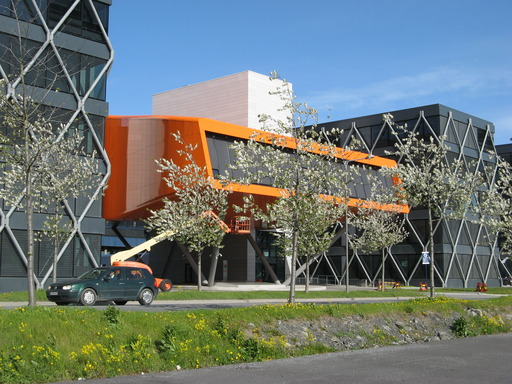
\includegraphics[keepaspectratio,width=9em,height=6em]{NorNet-Configuration-Images/Simula_Research_Laboratory.jpeg}} & \hyperref[sec:UiO]{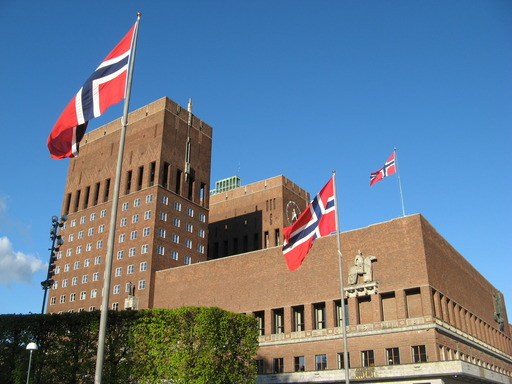
\includegraphics[keepaspectratio,width=9em,height=6em]{NorNet-Configuration-Images/Universitetet_i_Oslo.jpeg}} & \hyperref[sec:HiG]{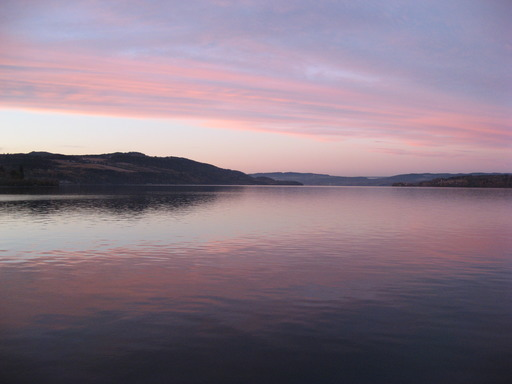
\includegraphics[keepaspectratio,width=9em,height=6em]{NorNet-Configuration-Images/Hoegskolen_i_Gjoevik.jpeg}} & \hyperref[sec:UiT]{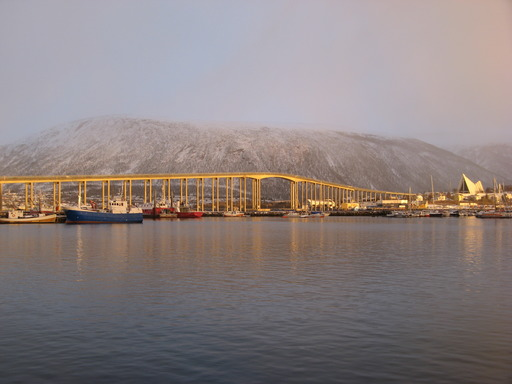
\includegraphics[keepaspectratio,width=9em,height=6em]{NorNet-Configuration-Images/Universitetet_i_Tromsoe.jpeg}} \\ \hline
 \hyperref[sec:UiS]{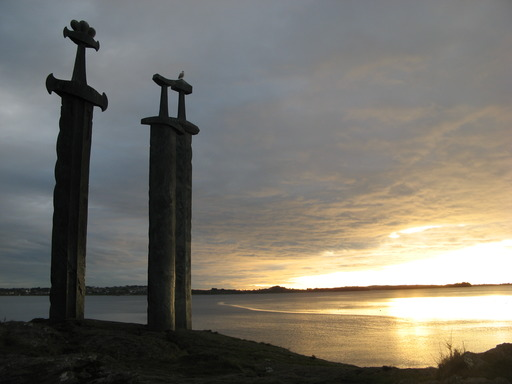
\includegraphics[keepaspectratio,width=9em,height=6em]{NorNet-Configuration-Images/Universitetet_i_Stavanger.jpeg}} & \hyperref[sec:UiB]{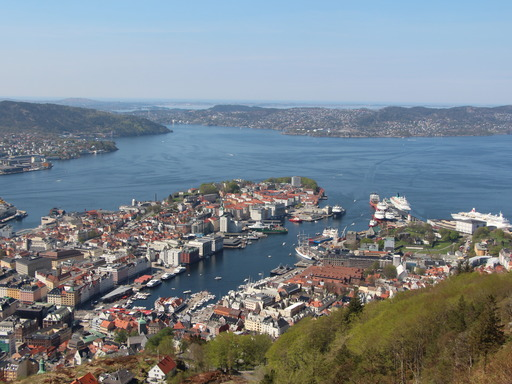
\includegraphics[keepaspectratio,width=9em,height=6em]{NorNet-Configuration-Images/Universitetet_i_Bergen.jpeg}} & \hyperref[sec:UiA]{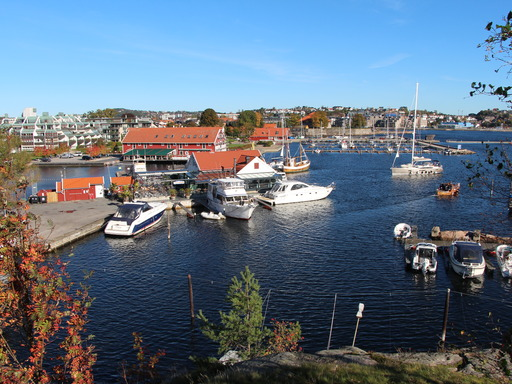
\includegraphics[keepaspectratio,width=9em,height=6em]{NorNet-Configuration-Images/Universitetet_i_Agder.jpeg}} & \hyperref[sec:UNIS]{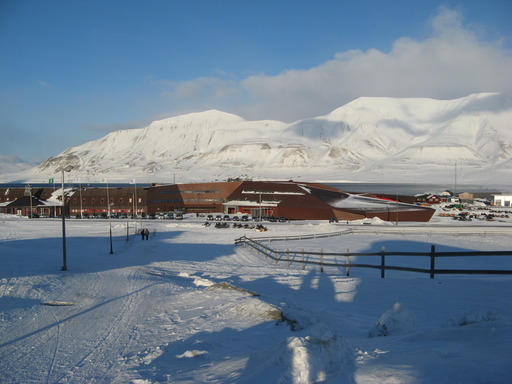
\includegraphics[keepaspectratio,width=9em,height=6em]{NorNet-Configuration-Images/Universitetet_paa_Svalbard.jpeg}} \\ \hline
 \hyperref[sec:NTNU]{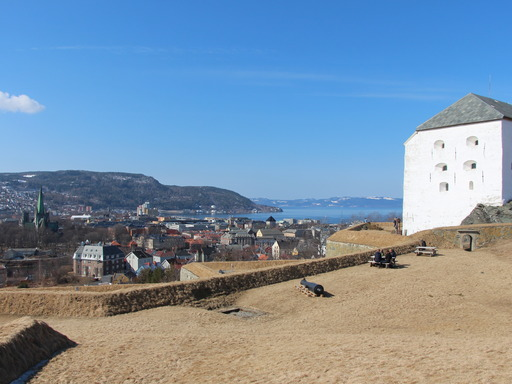
\includegraphics[keepaspectratio,width=9em,height=6em]{NorNet-Configuration-Images/Universitetet_i_Trondheim.jpeg}} & \hyperref[sec:HiN]{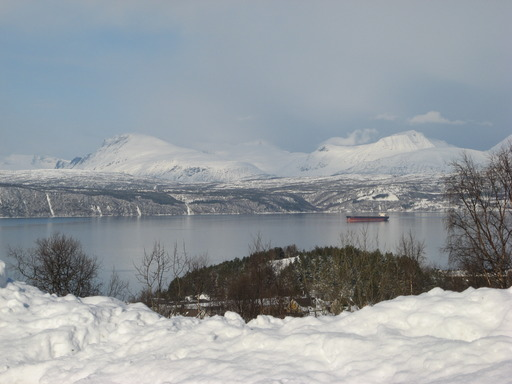
\includegraphics[keepaspectratio,width=9em,height=6em]{NorNet-Configuration-Images/Hoegskolen_i_Narvik.jpeg}} & \hyperref[sec:HiOA]{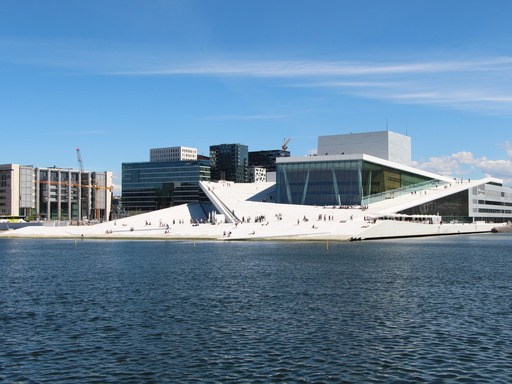
\includegraphics[keepaspectratio,width=9em,height=6em]{NorNet-Configuration-Images/Hoegskolen_i_Oslo_og_Akershus.jpeg}} & \hyperref[sec:KAU]{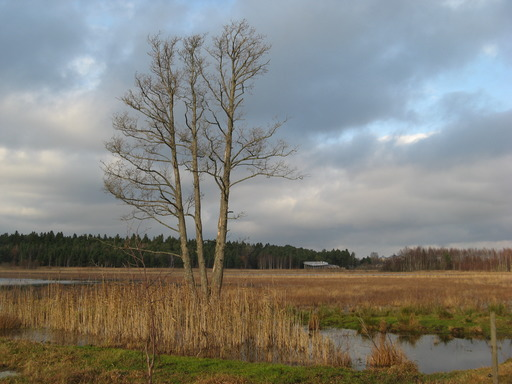
\includegraphics[keepaspectratio,width=9em,height=6em]{NorNet-Configuration-Images/Karlstads_Universitet.jpeg}} \\ \hline
 \hyperref[sec:TUKL]{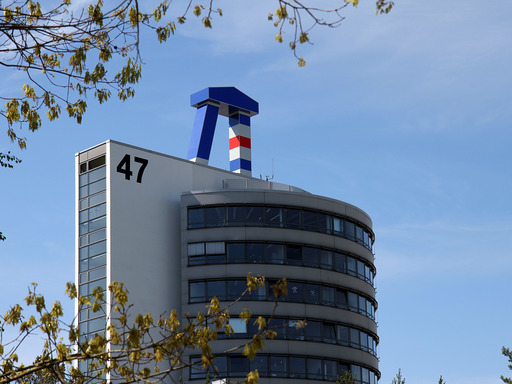
\includegraphics[keepaspectratio,width=9em,height=6em]{NorNet-Configuration-Images/Universitaet_Kaiserslautern.jpeg}} & \hyperref[sec:HAW]{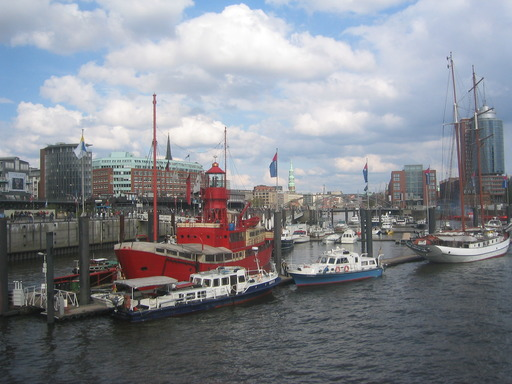
\includegraphics[keepaspectratio,width=9em,height=6em]{NorNet-Configuration-Images/Hochschule_Hamburg.jpeg}} & \hyperref[sec:UDE]{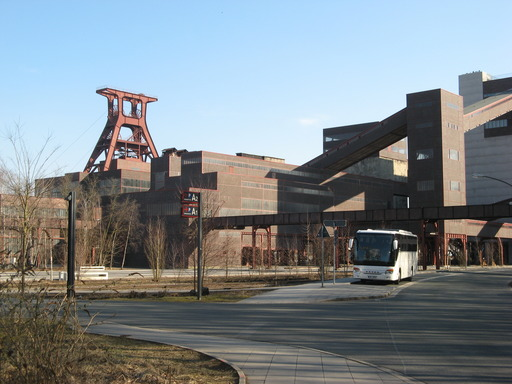
\includegraphics[keepaspectratio,width=9em,height=6em]{NorNet-Configuration-Images/Universitaet_Duisburg-Essen.jpeg}} & \hyperref[sec:TUDA]{\includegraphics[keepaspectratio,width=9em,height=6em]{NorNet-Configuration-Images/Universitaet_Darmstadt.jpeg}} \\ \hline
 \hyperref[sec:HU]{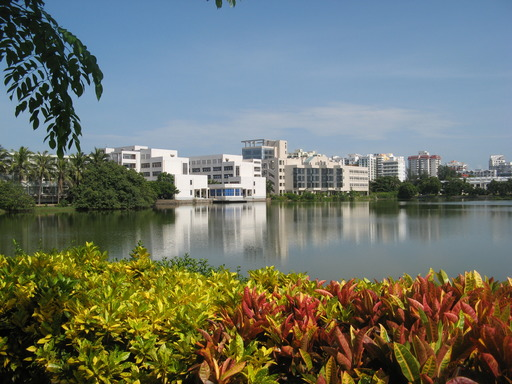
\includegraphics[keepaspectratio,width=9em,height=6em]{NorNet-Configuration-Images/Hainan_University.jpeg}} & \hyperref[sec:HKC]{\includegraphics[keepaspectratio,width=9em,height=6em]{NorNet-Configuration-Images/Haikou_College_of_Economics.jpeg}} & \hyperref[sec:KU]{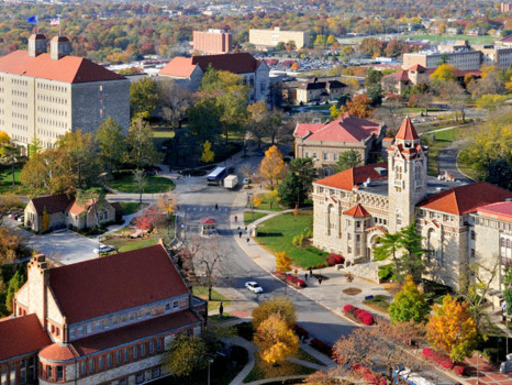
\includegraphics[keepaspectratio,width=9em,height=6em]{NorNet-Configuration-Images/The_University_of_Kansas.jpeg}} & \hyperref[sec:NYU]{\includegraphics[keepaspectratio,width=9em,height=6em]{NorNet-Configuration-Images/New_York_University.jpeg}} \\ \hline
 \hyperref[sec:KRU]{\includegraphics[keepaspectratio,width=9em,height=6em]{NorNet-Configuration-Images/Korea_University.jpeg}} & \hyperref[sec:NICTA]{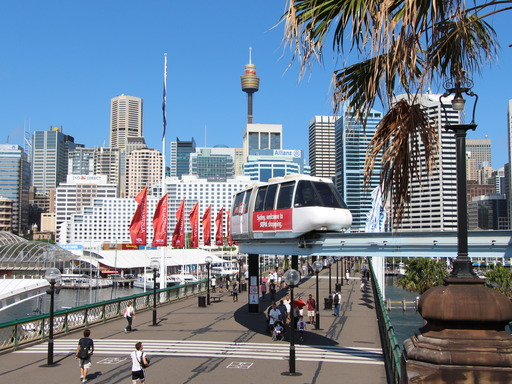
\includegraphics[keepaspectratio,width=9em,height=6em]{NorNet-Configuration-Images/National_ICT_Australia.jpeg}} &  &  \\ \hline
\end{longtable}
\end{center}
\end{small}
% %%%%%%%%%%%%%%%%%%%%%%%%%%%%%%%%%%%%%%%%%%%%%%%%%%%%%%%%%%%%%%%%%%%%%%%%%%%%




% @@@@@@@@@@@@@@@@@@@@@@@@@@@@@@@@@@@@@@@@@@@@@@@@@@@@@@@@@@@@@@@@@@@@@@@@@@@@
\chapter{Site Details}
\label{cha:Site-Details}
% @@@@@@@@@@@@@@@@@@@@@@@@@@@@@@@@@@@@@@@@@@@@@@@@@@@@@@@@@@@@@@@@@@@@@@@@@@@@




% ############################################################################
\section{Simula Research Laboratory (1)}
\label{sec:SRL}
% ############################################################################

Contacts:\begin{enumerate}
 \item \index{Dreibholz, Thomas}\href{mailto:dreibh@simula.no}{Thomas Dreibholz (dreibh@simula.no)}
 \item \index{Elmokashfi, Ahmed}\href{mailto:ahmed@simula.no}{Ahmed Elmokashfi (ahmed@simula.no)}
 \item \index{Werme, Jonas}\href{mailto:jonasw@simula.no}{Jonas Werme (jonasw@simula.no)}
\end{enumerate}

% %%%%%%%%%%%%%%%%%%%%%%%%%%%%%%%%%%%%%%%%%%%%%%%%%%%%%%%%%%%%%%%%%%%%%%%%%%%%
\begin{small}
\begin{center}
\begin{longtable}{|c|c|c|c|c|c|c|c|}
 \hline
 \multicolumn{8}{|c|}{\index{Simula Research Laboratory}\textbf{Simula Research Laboratory}} \\ \hline
 \multicolumn{4}{|c|}{\multirow{7}{*}{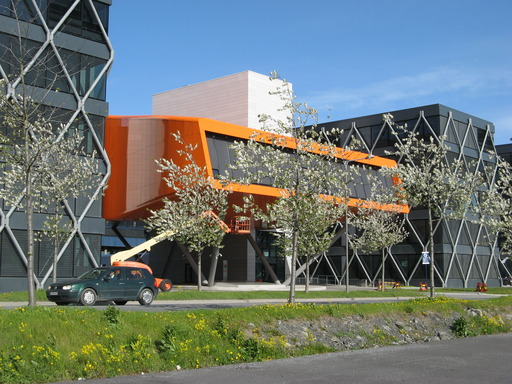
\includegraphics[keepaspectratio,height=7.75em]{NorNet-Configuration-Images/Simula_Research_Laboratory.jpeg}}} & \multicolumn{1}{|l|}{City} & \multicolumn{3}{|l|}{\index{Fornebu}Fornebu} \\* \cline{5-5}\cline{6-6}\cline{7-7}\cline{8-8}
 \multicolumn{4}{|c|}{} & \multicolumn{1}{|l|}{Province} & \multicolumn{3}{|l|}{\index{Akershus}
\includegraphics[keepaspectratio,height=0.8em]{NorNet-Configuration-Images/NO-Akershus.pdf}Akershus} \\* \cline{5-5}\cline{6-6}\cline{7-7}\cline{8-8}
 \multicolumn{4}{|c|}{} & \multicolumn{1}{|l|}{Country} & \multicolumn{3}{|l|}{\nomenclature{NO}{Norge}\index{NO|see{Norge}}\index{Norge}
\includegraphics[keepaspectratio,height=0.8em]{NorNet-Configuration-Images/Flag-NO.pdf}Norge (NO)} \\* \cline{5-5}\cline{6-6}\cline{7-7}\cline{8-8}
 \multicolumn{4}{|c|}{} & \multicolumn{1}{|l|}{GPS/ГЛОНАСС} & \multicolumn{3}{|l|}{59.8959°N / 10.6276°E / 15.0m} \\* \cline{5-5}\cline{6-6}\cline{7-7}\cline{8-8}
 \multicolumn{4}{|c|}{} & \multicolumn{1}{|l|}{Short Name} & \multicolumn{3}{|l|}{\nomenclature{SRL}{Simula Research Laboratory}\index{SRL|see{Simula Research Laboratory}}SRL} \\* \cline{5-5}\cline{6-6}\cline{7-7}\cline{8-8}
 \multicolumn{4}{|c|}{} & \multicolumn{1}{|l|}{Domain} & \multicolumn{3}{|l|}{\index{simula.nornet}simula.nornet} \\* \cline{5-5}\cline{6-6}\cline{7-7}\cline{8-8}
 \multicolumn{4}{|c|}{} & \multicolumn{1}{|l|}{URL} & \multicolumn{3}{|l|}{\url{https://www.simula.no}} \\ \hline
 \multicolumn{2}{|p{8em}|}{Node} & \multicolumn{2}{|p{8em}|}{Sliver} & \multicolumn{2}{|p{8em}|}{Provider} & IPv4 & IPv6 \\ \hline
\endfirsthead
\hline
 \multicolumn{8}{|c|}{\textbf{Simula Research Laboratory (continued)}} \\ \hline
 \multicolumn{2}{|p{8em}|}{Node} & \multicolumn{2}{|p{8em}|}{Sliver} & \multicolumn{2}{|p{8em}|}{Provider} & IPv4 & IPv6 \\ \hline
\endhead
 \multirow{16}{*}{\tiny{1}} & \multicolumn{3}{|c|}{\multirow{16}{*}{\tiny{tunnelbox}}} & \multicolumn{2}{|c|}{\multirow{4}{*}{\tiny{\href{https://www.uninett.no}{Uninett} (1)}}} & \tiny{158.39.4.2} & \tiny{2001:700:4100:4::2} \\* \cline{7-7}\cline{8-8}
  & \multicolumn{3}{|c|}{} & \multicolumn{2}{|c|}{} & \tiny{10.1.1.1} & \tiny{2001:700:4100:101::1} \\* \cline{7-7}\cline{8-8}
  & \multicolumn{3}{|c|}{} & \multicolumn{2}{|c|}{} & Type: & fibre, business \\* \cline{7-7}\cline{8-8}
  & \multicolumn{3}{|c|}{} & \multicolumn{2}{|c|}{} & Down/Up:  & unspecified \\* \cline{5-5}\cline{6-6}\cline{7-7}\cline{8-8}
  & \multicolumn{3}{|c|}{} & \multicolumn{2}{|c|}{\multirow{4}{*}{\tiny{\href{http://kvantel.no}{Kvantel} (2)}}} & \tiny{77.88.71.151} & \tiny{2a02:270:2014:111:77:88:71:151} \\* \cline{7-7}\cline{8-8}
  & \multicolumn{3}{|c|}{} & \multicolumn{2}{|c|}{} & \tiny{10.2.1.1} & \tiny{2001:700:4100:201::1} \\* \cline{7-7}\cline{8-8}
  & \multicolumn{3}{|c|}{} & \multicolumn{2}{|c|}{} & Type: & fibre, business \\* \cline{7-7}\cline{8-8}
  & \multicolumn{3}{|c|}{} & \multicolumn{2}{|c|}{} & Down/Up:  & unspecified \\* \cline{5-5}\cline{6-6}\cline{7-7}\cline{8-8}
  & \multicolumn{3}{|c|}{} & \multicolumn{2}{|c|}{\multirow{4}{*}{\tiny{\href{https://www.telenor.no}{Telenor} (4)}}} & \tiny{62.92.88.42} & \frownie{} \\* \cline{7-7}\cline{8-8}
  & \multicolumn{3}{|c|}{} & \multicolumn{2}{|c|}{} & \tiny{10.4.1.1} & \tiny{2001:700:4100:401::1} \\* \cline{7-7}\cline{8-8}
  & \multicolumn{3}{|c|}{} & \multicolumn{2}{|c|}{} & Type: & ADSL, consumer \\* \cline{7-7}\cline{8-8}
  & \multicolumn{3}{|c|}{} & \multicolumn{2}{|c|}{} & Down/Up:  & unspecified \\* \cline{5-5}\cline{6-6}\cline{7-7}\cline{8-8}
  & \multicolumn{3}{|c|}{} & \multicolumn{2}{|c|}{\multirow{4}{*}{\tiny{\href{http://www.powertech.no}{PowerTech} (9)}}} & \tiny{80.241.88.26} & \tiny{2001:840:4ad5::34} \\* \cline{7-7}\cline{8-8}
  & \multicolumn{3}{|c|}{} & \multicolumn{2}{|c|}{} & \tiny{10.9.1.1} & \tiny{2001:700:4100:901::1} \\* \cline{7-7}\cline{8-8}
  & \multicolumn{3}{|c|}{} & \multicolumn{2}{|c|}{} & Type: & ADSL, consumer \\* \cline{7-7}\cline{8-8}
  & \multicolumn{3}{|c|}{} & \multicolumn{2}{|c|}{} & Down/Up:  & unspecified \\ \hline
 \multirow{32}{*}{\tiny{100}} & \multicolumn{1}{|l|}{\multirow{32}{*}{\tiny{akerbrygge}}} & \multicolumn{2}{|c|}{\multirow{4}{*}{\tiny{Root Context}}} & \multicolumn{2}{|c|}{\tiny{\href{https://www.uninett.no}{Uninett} (1)}} & \tiny{10.1.1.100} & \tiny{2001:700:4100:101::64} \\* \cline{5-5}\cline{6-6}\cline{7-7}\cline{8-8}
  &  & \multicolumn{2}{|c|}{} & \multicolumn{2}{|c|}{\tiny{\href{http://kvantel.no}{Kvantel} (2)}} & \tiny{10.2.1.100} & \tiny{2001:700:4100:201::64} \\* \cline{5-5}\cline{6-6}\cline{7-7}\cline{8-8}
  &  & \multicolumn{2}{|c|}{} & \multicolumn{2}{|c|}{\tiny{\href{https://www.telenor.no}{Telenor} (4)}} & \tiny{10.4.1.100} & \tiny{2001:700:4100:401::64} \\* \cline{5-5}\cline{6-6}\cline{7-7}\cline{8-8}
  &  & \multicolumn{2}{|c|}{} & \multicolumn{2}{|c|}{\tiny{\href{http://www.powertech.no}{PowerTech} (9)}} & \tiny{10.9.1.100} & \tiny{2001:700:4100:901::64} \\* \cline{3-3}\cline{4-4}\cline{5-5}\cline{6-6}\cline{7-7}\cline{8-8}
  &  & \multirow{4}{*}{\tiny{116}} & \multicolumn{1}{|l|}{\multirow{4}{*}{\tiny{ude-delaytest}}} & \multicolumn{2}{|c|}{\tiny{\href{https://www.uninett.no}{Uninett} (1)}} & \tiny{10.1.1.116} & \tiny{2001:700:4100:101::74:64} \\* \cline{5-5}\cline{6-6}\cline{7-7}\cline{8-8}
  &  &  &  & \multicolumn{2}{|c|}{\tiny{\href{http://kvantel.no}{Kvantel} (2)}} & \tiny{10.2.1.116} & \tiny{2001:700:4100:201::74:64} \\* \cline{5-5}\cline{6-6}\cline{7-7}\cline{8-8}
  &  &  &  & \multicolumn{2}{|c|}{\tiny{\href{https://www.telenor.no}{Telenor} (4)}} & \tiny{10.4.1.116} & \tiny{2001:700:4100:401::74:64} \\* \cline{5-5}\cline{6-6}\cline{7-7}\cline{8-8}
  &  &  &  & \multicolumn{2}{|c|}{\tiny{\href{http://www.powertech.no}{PowerTech} (9)}} & \tiny{10.9.1.116} & \tiny{2001:700:4100:901::74:64} \\* \cline{3-3}\cline{4-4}\cline{5-5}\cline{6-6}\cline{7-7}\cline{8-8}
  &  & \multirow{4}{*}{\tiny{126}} & \multicolumn{1}{|l|}{\multirow{4}{*}{\tiny{srl-test}}} & \multicolumn{2}{|c|}{\tiny{\href{https://www.uninett.no}{Uninett} (1)}} & \tiny{10.1.1.126} & \tiny{2001:700:4100:101::7e:64} \\* \cline{5-5}\cline{6-6}\cline{7-7}\cline{8-8}
  &  &  &  & \multicolumn{2}{|c|}{\tiny{\href{http://kvantel.no}{Kvantel} (2)}} & \tiny{10.2.1.126} & \tiny{2001:700:4100:201::7e:64} \\* \cline{5-5}\cline{6-6}\cline{7-7}\cline{8-8}
  &  &  &  & \multicolumn{2}{|c|}{\tiny{\href{https://www.telenor.no}{Telenor} (4)}} & \tiny{10.4.1.126} & \tiny{2001:700:4100:401::7e:64} \\* \cline{5-5}\cline{6-6}\cline{7-7}\cline{8-8}
  &  &  &  & \multicolumn{2}{|c|}{\tiny{\href{http://www.powertech.no}{PowerTech} (9)}} & \tiny{10.9.1.126} & \tiny{2001:700:4100:901::7e:64} \\* \cline{3-3}\cline{4-4}\cline{5-5}\cline{6-6}\cline{7-7}\cline{8-8}
  &  & \multirow{4}{*}{\tiny{147}} & \multicolumn{1}{|l|}{\multirow{4}{*}{\tiny{haw-cmt}}} & \multicolumn{2}{|c|}{\tiny{\href{https://www.uninett.no}{Uninett} (1)}} & \tiny{10.1.1.147} & \tiny{2001:700:4100:101::93:64} \\* \cline{5-5}\cline{6-6}\cline{7-7}\cline{8-8}
  &  &  &  & \multicolumn{2}{|c|}{\tiny{\href{http://kvantel.no}{Kvantel} (2)}} & \tiny{10.2.1.147} & \tiny{2001:700:4100:201::93:64} \\* \cline{5-5}\cline{6-6}\cline{7-7}\cline{8-8}
  &  &  &  & \multicolumn{2}{|c|}{\tiny{\href{https://www.telenor.no}{Telenor} (4)}} & \tiny{10.4.1.147} & \tiny{2001:700:4100:401::93:64} \\* \cline{5-5}\cline{6-6}\cline{7-7}\cline{8-8}
  &  &  &  & \multicolumn{2}{|c|}{\tiny{\href{http://www.powertech.no}{PowerTech} (9)}} & \tiny{10.9.1.147} & \tiny{2001:700:4100:901::93:64} \\* \cline{3-3}\cline{4-4}\cline{5-5}\cline{6-6}\cline{7-7}\cline{8-8}
  &  & \multirow{4}{*}{\tiny{180}} & \multicolumn{1}{|l|}{\multirow{4}{*}{\tiny{hu-tanqilin}}} & \multicolumn{2}{|c|}{\tiny{\href{https://www.uninett.no}{Uninett} (1)}} & \tiny{10.1.1.180} & \tiny{2001:700:4100:101::b4:64} \\* \cline{5-5}\cline{6-6}\cline{7-7}\cline{8-8}
  &  &  &  & \multicolumn{2}{|c|}{\tiny{\href{http://kvantel.no}{Kvantel} (2)}} & \tiny{10.2.1.180} & \tiny{2001:700:4100:201::b4:64} \\* \cline{5-5}\cline{6-6}\cline{7-7}\cline{8-8}
  &  &  &  & \multicolumn{2}{|c|}{\tiny{\href{https://www.telenor.no}{Telenor} (4)}} & \tiny{10.4.1.180} & \tiny{2001:700:4100:401::b4:64} \\* \cline{5-5}\cline{6-6}\cline{7-7}\cline{8-8}
  &  &  &  & \multicolumn{2}{|c|}{\tiny{\href{http://www.powertech.no}{PowerTech} (9)}} & \tiny{10.9.1.180} & \tiny{2001:700:4100:901::b4:64} \\* \cline{3-3}\cline{4-4}\cline{5-5}\cline{6-6}\cline{7-7}\cline{8-8}
  &  & \multirow{4}{*}{\tiny{195}} & \multicolumn{1}{|l|}{\multirow{4}{*}{\tiny{hu-zhoufeng}}} & \multicolumn{2}{|c|}{\tiny{\href{https://www.uninett.no}{Uninett} (1)}} & \tiny{10.1.1.195} & \tiny{2001:700:4100:101::c3:64} \\* \cline{5-5}\cline{6-6}\cline{7-7}\cline{8-8}
  &  &  &  & \multicolumn{2}{|c|}{\tiny{\href{http://kvantel.no}{Kvantel} (2)}} & \tiny{10.2.1.195} & \tiny{2001:700:4100:201::c3:64} \\* \cline{5-5}\cline{6-6}\cline{7-7}\cline{8-8}
  &  &  &  & \multicolumn{2}{|c|}{\tiny{\href{https://www.telenor.no}{Telenor} (4)}} & \tiny{10.4.1.195} & \tiny{2001:700:4100:401::c3:64} \\* \cline{5-5}\cline{6-6}\cline{7-7}\cline{8-8}
  &  &  &  & \multicolumn{2}{|c|}{\tiny{\href{http://www.powertech.no}{PowerTech} (9)}} & \tiny{10.9.1.195} & \tiny{2001:700:4100:901::c3:64} \\* \cline{3-3}\cline{4-4}\cline{5-5}\cline{6-6}\cline{7-7}\cline{8-8}
  &  & \multirow{4}{*}{\tiny{199}} & \multicolumn{1}{|l|}{\multirow{4}{*}{\tiny{tuda-sereon}}} & \multicolumn{2}{|c|}{\tiny{\href{https://www.uninett.no}{Uninett} (1)}} & \tiny{10.1.1.199} & \tiny{2001:700:4100:101::c7:64} \\* \cline{5-5}\cline{6-6}\cline{7-7}\cline{8-8}
  &  &  &  & \multicolumn{2}{|c|}{\tiny{\href{http://kvantel.no}{Kvantel} (2)}} & \tiny{10.2.1.199} & \tiny{2001:700:4100:201::c7:64} \\* \cline{5-5}\cline{6-6}\cline{7-7}\cline{8-8}
  &  &  &  & \multicolumn{2}{|c|}{\tiny{\href{https://www.telenor.no}{Telenor} (4)}} & \tiny{10.4.1.199} & \tiny{2001:700:4100:401::c7:64} \\* \cline{5-5}\cline{6-6}\cline{7-7}\cline{8-8}
  &  &  &  & \multicolumn{2}{|c|}{\tiny{\href{http://www.powertech.no}{PowerTech} (9)}} & \tiny{10.9.1.199} & \tiny{2001:700:4100:901::c7:64} \\* \cline{3-3}\cline{4-4}\cline{5-5}\cline{6-6}\cline{7-7}\cline{8-8}
  &  & \multirow{4}{*}{\tiny{205}} & \multicolumn{1}{|l|}{\multirow{4}{*}{\tiny{ntnu-test}}} & \multicolumn{2}{|c|}{\tiny{\href{https://www.uninett.no}{Uninett} (1)}} & \tiny{10.1.1.205} & \tiny{2001:700:4100:101::cd:64} \\* \cline{5-5}\cline{6-6}\cline{7-7}\cline{8-8}
  &  &  &  & \multicolumn{2}{|c|}{\tiny{\href{http://kvantel.no}{Kvantel} (2)}} & \tiny{10.2.1.205} & \tiny{2001:700:4100:201::cd:64} \\* \cline{5-5}\cline{6-6}\cline{7-7}\cline{8-8}
  &  &  &  & \multicolumn{2}{|c|}{\tiny{\href{https://www.telenor.no}{Telenor} (4)}} & \tiny{10.4.1.205} & \tiny{2001:700:4100:401::cd:64} \\* \cline{5-5}\cline{6-6}\cline{7-7}\cline{8-8}
  &  &  &  & \multicolumn{2}{|c|}{\tiny{\href{http://www.powertech.no}{PowerTech} (9)}} & \tiny{10.9.1.205} & \tiny{2001:700:4100:901::cd:64} \\ \hline
 \multirow{48}{*}{\tiny{101}} & \multicolumn{1}{|l|}{\multirow{48}{*}{\tiny{bygdoey}}} & \multicolumn{2}{|c|}{\multirow{4}{*}{\tiny{Root Context}}} & \multicolumn{2}{|c|}{\tiny{\href{https://www.uninett.no}{Uninett} (1)}} & \tiny{10.1.1.101} & \tiny{2001:700:4100:101::65} \\* \cline{5-5}\cline{6-6}\cline{7-7}\cline{8-8}
  &  & \multicolumn{2}{|c|}{} & \multicolumn{2}{|c|}{\tiny{\href{http://kvantel.no}{Kvantel} (2)}} & \tiny{10.2.1.101} & \tiny{2001:700:4100:201::65} \\* \cline{5-5}\cline{6-6}\cline{7-7}\cline{8-8}
  &  & \multicolumn{2}{|c|}{} & \multicolumn{2}{|c|}{\tiny{\href{https://www.telenor.no}{Telenor} (4)}} & \tiny{10.4.1.101} & \tiny{2001:700:4100:401::65} \\* \cline{5-5}\cline{6-6}\cline{7-7}\cline{8-8}
  &  & \multicolumn{2}{|c|}{} & \multicolumn{2}{|c|}{\tiny{\href{http://www.powertech.no}{PowerTech} (9)}} & \tiny{10.9.1.101} & \tiny{2001:700:4100:901::65} \\* \cline{3-3}\cline{4-4}\cline{5-5}\cline{6-6}\cline{7-7}\cline{8-8}
  &  & \multirow{4}{*}{\tiny{115}} & \multicolumn{1}{|l|}{\multirow{4}{*}{\tiny{ude-multipath}}} & \multicolumn{2}{|c|}{\tiny{\href{https://www.uninett.no}{Uninett} (1)}} & \tiny{10.1.1.115} & \tiny{2001:700:4100:101::73:65} \\* \cline{5-5}\cline{6-6}\cline{7-7}\cline{8-8}
  &  &  &  & \multicolumn{2}{|c|}{\tiny{\href{http://kvantel.no}{Kvantel} (2)}} & \tiny{10.2.1.115} & \tiny{2001:700:4100:201::73:65} \\* \cline{5-5}\cline{6-6}\cline{7-7}\cline{8-8}
  &  &  &  & \multicolumn{2}{|c|}{\tiny{\href{https://www.telenor.no}{Telenor} (4)}} & \tiny{10.4.1.115} & \tiny{2001:700:4100:401::73:65} \\* \cline{5-5}\cline{6-6}\cline{7-7}\cline{8-8}
  &  &  &  & \multicolumn{2}{|c|}{\tiny{\href{http://www.powertech.no}{PowerTech} (9)}} & \tiny{10.9.1.115} & \tiny{2001:700:4100:901::73:65} \\* \cline{3-3}\cline{4-4}\cline{5-5}\cline{6-6}\cline{7-7}\cline{8-8}
  &  & \multirow{4}{*}{\tiny{122}} & \multicolumn{1}{|l|}{\multirow{4}{*}{\tiny{srl-test}}} & \multicolumn{2}{|c|}{\tiny{\href{https://www.uninett.no}{Uninett} (1)}} & \tiny{10.1.1.122} & \tiny{2001:700:4100:101::7a:65} \\* \cline{5-5}\cline{6-6}\cline{7-7}\cline{8-8}
  &  &  &  & \multicolumn{2}{|c|}{\tiny{\href{http://kvantel.no}{Kvantel} (2)}} & \tiny{10.2.1.122} & \tiny{2001:700:4100:201::7a:65} \\* \cline{5-5}\cline{6-6}\cline{7-7}\cline{8-8}
  &  &  &  & \multicolumn{2}{|c|}{\tiny{\href{https://www.telenor.no}{Telenor} (4)}} & \tiny{10.4.1.122} & \tiny{2001:700:4100:401::7a:65} \\* \cline{5-5}\cline{6-6}\cline{7-7}\cline{8-8}
  &  &  &  & \multicolumn{2}{|c|}{\tiny{\href{http://www.powertech.no}{PowerTech} (9)}} & \tiny{10.9.1.122} & \tiny{2001:700:4100:901::7a:65} \\* \cline{3-3}\cline{4-4}\cline{5-5}\cline{6-6}\cline{7-7}\cline{8-8}
  &  & \multirow{4}{*}{\tiny{129}} & \multicolumn{1}{|l|}{\multirow{4}{*}{\tiny{hu-multipath}}} & \multicolumn{2}{|c|}{\tiny{\href{https://www.uninett.no}{Uninett} (1)}} & \tiny{10.1.1.129} & \tiny{2001:700:4100:101::81:65} \\* \cline{5-5}\cline{6-6}\cline{7-7}\cline{8-8}
  &  &  &  & \multicolumn{2}{|c|}{\tiny{\href{http://kvantel.no}{Kvantel} (2)}} & \tiny{10.2.1.129} & \tiny{2001:700:4100:201::81:65} \\* \cline{5-5}\cline{6-6}\cline{7-7}\cline{8-8}
  &  &  &  & \multicolumn{2}{|c|}{\tiny{\href{https://www.telenor.no}{Telenor} (4)}} & \tiny{10.4.1.129} & \tiny{2001:700:4100:401::81:65} \\* \cline{5-5}\cline{6-6}\cline{7-7}\cline{8-8}
  &  &  &  & \multicolumn{2}{|c|}{\tiny{\href{http://www.powertech.no}{PowerTech} (9)}} & \tiny{10.9.1.129} & \tiny{2001:700:4100:901::81:65} \\* \cline{3-3}\cline{4-4}\cline{5-5}\cline{6-6}\cline{7-7}\cline{8-8}
  &  & \multirow{4}{*}{\tiny{134}} & \multicolumn{1}{|l|}{\multirow{4}{*}{\tiny{haw-cmt}}} & \multicolumn{2}{|c|}{\tiny{\href{https://www.uninett.no}{Uninett} (1)}} & \tiny{10.1.1.134} & \tiny{2001:700:4100:101::86:65} \\* \cline{5-5}\cline{6-6}\cline{7-7}\cline{8-8}
  &  &  &  & \multicolumn{2}{|c|}{\tiny{\href{http://kvantel.no}{Kvantel} (2)}} & \tiny{10.2.1.134} & \tiny{2001:700:4100:201::86:65} \\* \cline{5-5}\cline{6-6}\cline{7-7}\cline{8-8}
  &  &  &  & \multicolumn{2}{|c|}{\tiny{\href{https://www.telenor.no}{Telenor} (4)}} & \tiny{10.4.1.134} & \tiny{2001:700:4100:401::86:65} \\* \cline{5-5}\cline{6-6}\cline{7-7}\cline{8-8}
  &  &  &  & \multicolumn{2}{|c|}{\tiny{\href{http://www.powertech.no}{PowerTech} (9)}} & \tiny{10.9.1.134} & \tiny{2001:700:4100:901::86:65} \\* \cline{3-3}\cline{4-4}\cline{5-5}\cline{6-6}\cline{7-7}\cline{8-8}
  &  & \multirow{4}{*}{\tiny{148}} & \multicolumn{1}{|l|}{\multirow{4}{*}{\tiny{srl-cps}}} & \multicolumn{2}{|c|}{\tiny{\href{https://www.uninett.no}{Uninett} (1)}} & \tiny{10.1.1.148} & \tiny{2001:700:4100:101::94:65} \\* \cline{5-5}\cline{6-6}\cline{7-7}\cline{8-8}
  &  &  &  & \multicolumn{2}{|c|}{\tiny{\href{http://kvantel.no}{Kvantel} (2)}} & \tiny{10.2.1.148} & \tiny{2001:700:4100:201::94:65} \\* \cline{5-5}\cline{6-6}\cline{7-7}\cline{8-8}
  &  &  &  & \multicolumn{2}{|c|}{\tiny{\href{https://www.telenor.no}{Telenor} (4)}} & \tiny{10.4.1.148} & \tiny{2001:700:4100:401::94:65} \\* \cline{5-5}\cline{6-6}\cline{7-7}\cline{8-8}
  &  &  &  & \multicolumn{2}{|c|}{\tiny{\href{http://www.powertech.no}{PowerTech} (9)}} & \tiny{10.9.1.148} & \tiny{2001:700:4100:901::94:65} \\* \cline{3-3}\cline{4-4}\cline{5-5}\cline{6-6}\cline{7-7}\cline{8-8}
  &  & \multirow{4}{*}{\tiny{155}} & \multicolumn{1}{|l|}{\multirow{4}{*}{\tiny{hu-tanqilin}}} & \multicolumn{2}{|c|}{\tiny{\href{https://www.uninett.no}{Uninett} (1)}} & \tiny{10.1.1.155} & \tiny{2001:700:4100:101::9b:65} \\* \cline{5-5}\cline{6-6}\cline{7-7}\cline{8-8}
  &  &  &  & \multicolumn{2}{|c|}{\tiny{\href{http://kvantel.no}{Kvantel} (2)}} & \tiny{10.2.1.155} & \tiny{2001:700:4100:201::9b:65} \\* \cline{5-5}\cline{6-6}\cline{7-7}\cline{8-8}
  &  &  &  & \multicolumn{2}{|c|}{\tiny{\href{https://www.telenor.no}{Telenor} (4)}} & \tiny{10.4.1.155} & \tiny{2001:700:4100:401::9b:65} \\* \cline{5-5}\cline{6-6}\cline{7-7}\cline{8-8}
  &  &  &  & \multicolumn{2}{|c|}{\tiny{\href{http://www.powertech.no}{PowerTech} (9)}} & \tiny{10.9.1.155} & \tiny{2001:700:4100:901::9b:65} \\* \cline{3-3}\cline{4-4}\cline{5-5}\cline{6-6}\cline{7-7}\cline{8-8}
  &  & \multirow{4}{*}{\tiny{161}} & \multicolumn{1}{|l|}{\multirow{4}{*}{\tiny{ntnu-test}}} & \multicolumn{2}{|c|}{\tiny{\href{https://www.uninett.no}{Uninett} (1)}} & \tiny{10.1.1.161} & \tiny{2001:700:4100:101::a1:65} \\* \cline{5-5}\cline{6-6}\cline{7-7}\cline{8-8}
  &  &  &  & \multicolumn{2}{|c|}{\tiny{\href{http://kvantel.no}{Kvantel} (2)}} & \tiny{10.2.1.161} & \tiny{2001:700:4100:201::a1:65} \\* \cline{5-5}\cline{6-6}\cline{7-7}\cline{8-8}
  &  &  &  & \multicolumn{2}{|c|}{\tiny{\href{https://www.telenor.no}{Telenor} (4)}} & \tiny{10.4.1.161} & \tiny{2001:700:4100:401::a1:65} \\* \cline{5-5}\cline{6-6}\cline{7-7}\cline{8-8}
  &  &  &  & \multicolumn{2}{|c|}{\tiny{\href{http://www.powertech.no}{PowerTech} (9)}} & \tiny{10.9.1.161} & \tiny{2001:700:4100:901::a1:65} \\* \cline{3-3}\cline{4-4}\cline{5-5}\cline{6-6}\cline{7-7}\cline{8-8}
  &  & \multirow{4}{*}{\tiny{174}} & \multicolumn{1}{|l|}{\multirow{4}{*}{\tiny{srl-netperformance}}} & \multicolumn{2}{|c|}{\tiny{\href{https://www.uninett.no}{Uninett} (1)}} & \tiny{10.1.1.174} & \tiny{2001:700:4100:101::ae:65} \\* \cline{5-5}\cline{6-6}\cline{7-7}\cline{8-8}
  &  &  &  & \multicolumn{2}{|c|}{\tiny{\href{http://kvantel.no}{Kvantel} (2)}} & \tiny{10.2.1.174} & \tiny{2001:700:4100:201::ae:65} \\* \cline{5-5}\cline{6-6}\cline{7-7}\cline{8-8}
  &  &  &  & \multicolumn{2}{|c|}{\tiny{\href{https://www.telenor.no}{Telenor} (4)}} & \tiny{10.4.1.174} & \tiny{2001:700:4100:401::ae:65} \\* \cline{5-5}\cline{6-6}\cline{7-7}\cline{8-8}
  &  &  &  & \multicolumn{2}{|c|}{\tiny{\href{http://www.powertech.no}{PowerTech} (9)}} & \tiny{10.9.1.174} & \tiny{2001:700:4100:901::ae:65} \\* \cline{3-3}\cline{4-4}\cline{5-5}\cline{6-6}\cline{7-7}\cline{8-8}
  &  & \multirow{4}{*}{\tiny{175}} & \multicolumn{1}{|l|}{\multirow{4}{*}{\tiny{hu-chengxi}}} & \multicolumn{2}{|c|}{\tiny{\href{https://www.uninett.no}{Uninett} (1)}} & \tiny{10.1.1.175} & \tiny{2001:700:4100:101::af:65} \\* \cline{5-5}\cline{6-6}\cline{7-7}\cline{8-8}
  &  &  &  & \multicolumn{2}{|c|}{\tiny{\href{http://kvantel.no}{Kvantel} (2)}} & \tiny{10.2.1.175} & \tiny{2001:700:4100:201::af:65} \\* \cline{5-5}\cline{6-6}\cline{7-7}\cline{8-8}
  &  &  &  & \multicolumn{2}{|c|}{\tiny{\href{https://www.telenor.no}{Telenor} (4)}} & \tiny{10.4.1.175} & \tiny{2001:700:4100:401::af:65} \\* \cline{5-5}\cline{6-6}\cline{7-7}\cline{8-8}
  &  &  &  & \multicolumn{2}{|c|}{\tiny{\href{http://www.powertech.no}{PowerTech} (9)}} & \tiny{10.9.1.175} & \tiny{2001:700:4100:901::af:65} \\* \cline{3-3}\cline{4-4}\cline{5-5}\cline{6-6}\cline{7-7}\cline{8-8}
  &  & \multirow{4}{*}{\tiny{176}} & \multicolumn{1}{|l|}{\multirow{4}{*}{\tiny{kau-mptcpsecurity}}} & \multicolumn{2}{|c|}{\tiny{\href{https://www.uninett.no}{Uninett} (1)}} & \tiny{10.1.1.176} & \tiny{2001:700:4100:101::b0:65} \\* \cline{5-5}\cline{6-6}\cline{7-7}\cline{8-8}
  &  &  &  & \multicolumn{2}{|c|}{\tiny{\href{http://kvantel.no}{Kvantel} (2)}} & \tiny{10.2.1.176} & \tiny{2001:700:4100:201::b0:65} \\* \cline{5-5}\cline{6-6}\cline{7-7}\cline{8-8}
  &  &  &  & \multicolumn{2}{|c|}{\tiny{\href{https://www.telenor.no}{Telenor} (4)}} & \tiny{10.4.1.176} & \tiny{2001:700:4100:401::b0:65} \\* \cline{5-5}\cline{6-6}\cline{7-7}\cline{8-8}
  &  &  &  & \multicolumn{2}{|c|}{\tiny{\href{http://www.powertech.no}{PowerTech} (9)}} & \tiny{10.9.1.176} & \tiny{2001:700:4100:901::b0:65} \\* \cline{3-3}\cline{4-4}\cline{5-5}\cline{6-6}\cline{7-7}\cline{8-8}
  &  & \multirow{4}{*}{\tiny{184}} & \multicolumn{1}{|l|}{\multirow{4}{*}{\tiny{tuda-sereon}}} & \multicolumn{2}{|c|}{\tiny{\href{https://www.uninett.no}{Uninett} (1)}} & \tiny{10.1.1.184} & \tiny{2001:700:4100:101::b8:65} \\* \cline{5-5}\cline{6-6}\cline{7-7}\cline{8-8}
  &  &  &  & \multicolumn{2}{|c|}{\tiny{\href{http://kvantel.no}{Kvantel} (2)}} & \tiny{10.2.1.184} & \tiny{2001:700:4100:201::b8:65} \\* \cline{5-5}\cline{6-6}\cline{7-7}\cline{8-8}
  &  &  &  & \multicolumn{2}{|c|}{\tiny{\href{https://www.telenor.no}{Telenor} (4)}} & \tiny{10.4.1.184} & \tiny{2001:700:4100:401::b8:65} \\* \cline{5-5}\cline{6-6}\cline{7-7}\cline{8-8}
  &  &  &  & \multicolumn{2}{|c|}{\tiny{\href{http://www.powertech.no}{PowerTech} (9)}} & \tiny{10.9.1.184} & \tiny{2001:700:4100:901::b8:65} \\ \hline
 \multirow{20}{*}{\tiny{102}} & \multicolumn{1}{|l|}{\multirow{20}{*}{\tiny{tullinloekka}}} & \multicolumn{2}{|c|}{\multirow{4}{*}{\tiny{Root Context}}} & \multicolumn{2}{|c|}{\tiny{\href{https://www.uninett.no}{Uninett} (1)}} & \tiny{10.1.1.102} & \tiny{2001:700:4100:101::66} \\* \cline{5-5}\cline{6-6}\cline{7-7}\cline{8-8}
  &  & \multicolumn{2}{|c|}{} & \multicolumn{2}{|c|}{\tiny{\href{http://kvantel.no}{Kvantel} (2)}} & \tiny{10.2.1.102} & \tiny{2001:700:4100:201::66} \\* \cline{5-5}\cline{6-6}\cline{7-7}\cline{8-8}
  &  & \multicolumn{2}{|c|}{} & \multicolumn{2}{|c|}{\tiny{\href{https://www.telenor.no}{Telenor} (4)}} & \tiny{10.4.1.102} & \tiny{2001:700:4100:401::66} \\* \cline{5-5}\cline{6-6}\cline{7-7}\cline{8-8}
  &  & \multicolumn{2}{|c|}{} & \multicolumn{2}{|c|}{\tiny{\href{http://www.powertech.no}{PowerTech} (9)}} & \tiny{10.9.1.102} & \tiny{2001:700:4100:901::66} \\* \cline{3-3}\cline{4-4}\cline{5-5}\cline{6-6}\cline{7-7}\cline{8-8}
  &  & \multirow{4}{*}{\tiny{127}} & \multicolumn{1}{|l|}{\multirow{4}{*}{\tiny{srl-test}}} & \multicolumn{2}{|c|}{\tiny{\href{https://www.uninett.no}{Uninett} (1)}} & \tiny{10.1.1.127} & \tiny{2001:700:4100:101::7f:66} \\* \cline{5-5}\cline{6-6}\cline{7-7}\cline{8-8}
  &  &  &  & \multicolumn{2}{|c|}{\tiny{\href{http://kvantel.no}{Kvantel} (2)}} & \tiny{10.2.1.127} & \tiny{2001:700:4100:201::7f:66} \\* \cline{5-5}\cline{6-6}\cline{7-7}\cline{8-8}
  &  &  &  & \multicolumn{2}{|c|}{\tiny{\href{https://www.telenor.no}{Telenor} (4)}} & \tiny{10.4.1.127} & \tiny{2001:700:4100:401::7f:66} \\* \cline{5-5}\cline{6-6}\cline{7-7}\cline{8-8}
  &  &  &  & \multicolumn{2}{|c|}{\tiny{\href{http://www.powertech.no}{PowerTech} (9)}} & \tiny{10.9.1.127} & \tiny{2001:700:4100:901::7f:66} \\* \cline{3-3}\cline{4-4}\cline{5-5}\cline{6-6}\cline{7-7}\cline{8-8}
  &  & \multirow{4}{*}{\tiny{137}} & \multicolumn{1}{|l|}{\multirow{4}{*}{\tiny{hu-multipath}}} & \multicolumn{2}{|c|}{\tiny{\href{https://www.uninett.no}{Uninett} (1)}} & \tiny{10.1.1.137} & \tiny{2001:700:4100:101::89:66} \\* \cline{5-5}\cline{6-6}\cline{7-7}\cline{8-8}
  &  &  &  & \multicolumn{2}{|c|}{\tiny{\href{http://kvantel.no}{Kvantel} (2)}} & \tiny{10.2.1.137} & \tiny{2001:700:4100:201::89:66} \\* \cline{5-5}\cline{6-6}\cline{7-7}\cline{8-8}
  &  &  &  & \multicolumn{2}{|c|}{\tiny{\href{https://www.telenor.no}{Telenor} (4)}} & \tiny{10.4.1.137} & \tiny{2001:700:4100:401::89:66} \\* \cline{5-5}\cline{6-6}\cline{7-7}\cline{8-8}
  &  &  &  & \multicolumn{2}{|c|}{\tiny{\href{http://www.powertech.no}{PowerTech} (9)}} & \tiny{10.9.1.137} & \tiny{2001:700:4100:901::89:66} \\* \cline{3-3}\cline{4-4}\cline{5-5}\cline{6-6}\cline{7-7}\cline{8-8}
  &  & \multirow{4}{*}{\tiny{166}} & \multicolumn{1}{|l|}{\multirow{4}{*}{\tiny{ntnu-test}}} & \multicolumn{2}{|c|}{\tiny{\href{https://www.uninett.no}{Uninett} (1)}} & \tiny{10.1.1.166} & \tiny{2001:700:4100:101::a6:66} \\* \cline{5-5}\cline{6-6}\cline{7-7}\cline{8-8}
  &  &  &  & \multicolumn{2}{|c|}{\tiny{\href{http://kvantel.no}{Kvantel} (2)}} & \tiny{10.2.1.166} & \tiny{2001:700:4100:201::a6:66} \\* \cline{5-5}\cline{6-6}\cline{7-7}\cline{8-8}
  &  &  &  & \multicolumn{2}{|c|}{\tiny{\href{https://www.telenor.no}{Telenor} (4)}} & \tiny{10.4.1.166} & \tiny{2001:700:4100:401::a6:66} \\* \cline{5-5}\cline{6-6}\cline{7-7}\cline{8-8}
  &  &  &  & \multicolumn{2}{|c|}{\tiny{\href{http://www.powertech.no}{PowerTech} (9)}} & \tiny{10.9.1.166} & \tiny{2001:700:4100:901::a6:66} \\* \cline{3-3}\cline{4-4}\cline{5-5}\cline{6-6}\cline{7-7}\cline{8-8}
  &  & \multirow{4}{*}{\tiny{172}} & \multicolumn{1}{|l|}{\multirow{4}{*}{\tiny{srl-thuen}}} & \multicolumn{2}{|c|}{\tiny{\href{https://www.uninett.no}{Uninett} (1)}} & \tiny{10.1.1.172} & \tiny{2001:700:4100:101::ac:66} \\* \cline{5-5}\cline{6-6}\cline{7-7}\cline{8-8}
  &  &  &  & \multicolumn{2}{|c|}{\tiny{\href{http://kvantel.no}{Kvantel} (2)}} & \tiny{10.2.1.172} & \tiny{2001:700:4100:201::ac:66} \\* \cline{5-5}\cline{6-6}\cline{7-7}\cline{8-8}
  &  &  &  & \multicolumn{2}{|c|}{\tiny{\href{https://www.telenor.no}{Telenor} (4)}} & \tiny{10.4.1.172} & \tiny{2001:700:4100:401::ac:66} \\* \cline{5-5}\cline{6-6}\cline{7-7}\cline{8-8}
  &  &  &  & \multicolumn{2}{|c|}{\tiny{\href{http://www.powertech.no}{PowerTech} (9)}} & \tiny{10.9.1.172} & \tiny{2001:700:4100:901::ac:66} \\ \hline
 \multirow{32}{*}{\tiny{103}} & \multicolumn{1}{|l|}{\multirow{32}{*}{\tiny{frogner}}} & \multicolumn{2}{|c|}{\multirow{4}{*}{\tiny{Root Context}}} & \multicolumn{2}{|c|}{\tiny{\href{https://www.uninett.no}{Uninett} (1)}} & \tiny{10.1.1.103} & \tiny{2001:700:4100:101::67} \\* \cline{5-5}\cline{6-6}\cline{7-7}\cline{8-8}
  &  & \multicolumn{2}{|c|}{} & \multicolumn{2}{|c|}{\tiny{\href{http://kvantel.no}{Kvantel} (2)}} & \tiny{10.2.1.103} & \tiny{2001:700:4100:201::67} \\* \cline{5-5}\cline{6-6}\cline{7-7}\cline{8-8}
  &  & \multicolumn{2}{|c|}{} & \multicolumn{2}{|c|}{\tiny{\href{https://www.telenor.no}{Telenor} (4)}} & \tiny{10.4.1.103} & \tiny{2001:700:4100:401::67} \\* \cline{5-5}\cline{6-6}\cline{7-7}\cline{8-8}
  &  & \multicolumn{2}{|c|}{} & \multicolumn{2}{|c|}{\tiny{\href{http://www.powertech.no}{PowerTech} (9)}} & \tiny{10.9.1.103} & \tiny{2001:700:4100:901::67} \\* \cline{3-3}\cline{4-4}\cline{5-5}\cline{6-6}\cline{7-7}\cline{8-8}
  &  & \multirow{4}{*}{\tiny{131}} & \multicolumn{1}{|l|}{\multirow{4}{*}{\tiny{srl-test}}} & \multicolumn{2}{|c|}{\tiny{\href{https://www.uninett.no}{Uninett} (1)}} & \tiny{10.1.1.131} & \tiny{2001:700:4100:101::83:67} \\* \cline{5-5}\cline{6-6}\cline{7-7}\cline{8-8}
  &  &  &  & \multicolumn{2}{|c|}{\tiny{\href{http://kvantel.no}{Kvantel} (2)}} & \tiny{10.2.1.131} & \tiny{2001:700:4100:201::83:67} \\* \cline{5-5}\cline{6-6}\cline{7-7}\cline{8-8}
  &  &  &  & \multicolumn{2}{|c|}{\tiny{\href{https://www.telenor.no}{Telenor} (4)}} & \tiny{10.4.1.131} & \tiny{2001:700:4100:401::83:67} \\* \cline{5-5}\cline{6-6}\cline{7-7}\cline{8-8}
  &  &  &  & \multicolumn{2}{|c|}{\tiny{\href{http://www.powertech.no}{PowerTech} (9)}} & \tiny{10.9.1.131} & \tiny{2001:700:4100:901::83:67} \\* \cline{3-3}\cline{4-4}\cline{5-5}\cline{6-6}\cline{7-7}\cline{8-8}
  &  & \multirow{4}{*}{\tiny{133}} & \multicolumn{1}{|l|}{\multirow{4}{*}{\tiny{srl-queuing}}} & \multicolumn{2}{|c|}{\tiny{\href{https://www.uninett.no}{Uninett} (1)}} & \tiny{10.1.1.133} & \tiny{2001:700:4100:101::85:67} \\* \cline{5-5}\cline{6-6}\cline{7-7}\cline{8-8}
  &  &  &  & \multicolumn{2}{|c|}{\tiny{\href{http://kvantel.no}{Kvantel} (2)}} & \tiny{10.2.1.133} & \tiny{2001:700:4100:201::85:67} \\* \cline{5-5}\cline{6-6}\cline{7-7}\cline{8-8}
  &  &  &  & \multicolumn{2}{|c|}{\tiny{\href{https://www.telenor.no}{Telenor} (4)}} & \tiny{10.4.1.133} & \tiny{2001:700:4100:401::85:67} \\* \cline{5-5}\cline{6-6}\cline{7-7}\cline{8-8}
  &  &  &  & \multicolumn{2}{|c|}{\tiny{\href{http://www.powertech.no}{PowerTech} (9)}} & \tiny{10.9.1.133} & \tiny{2001:700:4100:901::85:67} \\* \cline{3-3}\cline{4-4}\cline{5-5}\cline{6-6}\cline{7-7}\cline{8-8}
  &  & \multirow{4}{*}{\tiny{145}} & \multicolumn{1}{|l|}{\multirow{4}{*}{\tiny{hu-multipath}}} & \multicolumn{2}{|c|}{\tiny{\href{https://www.uninett.no}{Uninett} (1)}} & \tiny{10.1.1.145} & \tiny{2001:700:4100:101::91:67} \\* \cline{5-5}\cline{6-6}\cline{7-7}\cline{8-8}
  &  &  &  & \multicolumn{2}{|c|}{\tiny{\href{http://kvantel.no}{Kvantel} (2)}} & \tiny{10.2.1.145} & \tiny{2001:700:4100:201::91:67} \\* \cline{5-5}\cline{6-6}\cline{7-7}\cline{8-8}
  &  &  &  & \multicolumn{2}{|c|}{\tiny{\href{https://www.telenor.no}{Telenor} (4)}} & \tiny{10.4.1.145} & \tiny{2001:700:4100:401::91:67} \\* \cline{5-5}\cline{6-6}\cline{7-7}\cline{8-8}
  &  &  &  & \multicolumn{2}{|c|}{\tiny{\href{http://www.powertech.no}{PowerTech} (9)}} & \tiny{10.9.1.145} & \tiny{2001:700:4100:901::91:67} \\* \cline{3-3}\cline{4-4}\cline{5-5}\cline{6-6}\cline{7-7}\cline{8-8}
  &  & \multirow{4}{*}{\tiny{170}} & \multicolumn{1}{|l|}{\multirow{4}{*}{\tiny{ntnu-test}}} & \multicolumn{2}{|c|}{\tiny{\href{https://www.uninett.no}{Uninett} (1)}} & \tiny{10.1.1.170} & \tiny{2001:700:4100:101::aa:67} \\* \cline{5-5}\cline{6-6}\cline{7-7}\cline{8-8}
  &  &  &  & \multicolumn{2}{|c|}{\tiny{\href{http://kvantel.no}{Kvantel} (2)}} & \tiny{10.2.1.170} & \tiny{2001:700:4100:201::aa:67} \\* \cline{5-5}\cline{6-6}\cline{7-7}\cline{8-8}
  &  &  &  & \multicolumn{2}{|c|}{\tiny{\href{https://www.telenor.no}{Telenor} (4)}} & \tiny{10.4.1.170} & \tiny{2001:700:4100:401::aa:67} \\* \cline{5-5}\cline{6-6}\cline{7-7}\cline{8-8}
  &  &  &  & \multicolumn{2}{|c|}{\tiny{\href{http://www.powertech.no}{PowerTech} (9)}} & \tiny{10.9.1.170} & \tiny{2001:700:4100:901::aa:67} \\* \cline{3-3}\cline{4-4}\cline{5-5}\cline{6-6}\cline{7-7}\cline{8-8}
  &  & \multirow{4}{*}{\tiny{177}} & \multicolumn{1}{|l|}{\multirow{4}{*}{\tiny{hu-chengxi}}} & \multicolumn{2}{|c|}{\tiny{\href{https://www.uninett.no}{Uninett} (1)}} & \tiny{10.1.1.177} & \tiny{2001:700:4100:101::b1:67} \\* \cline{5-5}\cline{6-6}\cline{7-7}\cline{8-8}
  &  &  &  & \multicolumn{2}{|c|}{\tiny{\href{http://kvantel.no}{Kvantel} (2)}} & \tiny{10.2.1.177} & \tiny{2001:700:4100:201::b1:67} \\* \cline{5-5}\cline{6-6}\cline{7-7}\cline{8-8}
  &  &  &  & \multicolumn{2}{|c|}{\tiny{\href{https://www.telenor.no}{Telenor} (4)}} & \tiny{10.4.1.177} & \tiny{2001:700:4100:401::b1:67} \\* \cline{5-5}\cline{6-6}\cline{7-7}\cline{8-8}
  &  &  &  & \multicolumn{2}{|c|}{\tiny{\href{http://www.powertech.no}{PowerTech} (9)}} & \tiny{10.9.1.177} & \tiny{2001:700:4100:901::b1:67} \\* \cline{3-3}\cline{4-4}\cline{5-5}\cline{6-6}\cline{7-7}\cline{8-8}
  &  & \multirow{4}{*}{\tiny{185}} & \multicolumn{1}{|l|}{\multirow{4}{*}{\tiny{hu-xingzhou}}} & \multicolumn{2}{|c|}{\tiny{\href{https://www.uninett.no}{Uninett} (1)}} & \tiny{10.1.1.185} & \tiny{2001:700:4100:101::b9:67} \\* \cline{5-5}\cline{6-6}\cline{7-7}\cline{8-8}
  &  &  &  & \multicolumn{2}{|c|}{\tiny{\href{http://kvantel.no}{Kvantel} (2)}} & \tiny{10.2.1.185} & \tiny{2001:700:4100:201::b9:67} \\* \cline{5-5}\cline{6-6}\cline{7-7}\cline{8-8}
  &  &  &  & \multicolumn{2}{|c|}{\tiny{\href{https://www.telenor.no}{Telenor} (4)}} & \tiny{10.4.1.185} & \tiny{2001:700:4100:401::b9:67} \\* \cline{5-5}\cline{6-6}\cline{7-7}\cline{8-8}
  &  &  &  & \multicolumn{2}{|c|}{\tiny{\href{http://www.powertech.no}{PowerTech} (9)}} & \tiny{10.9.1.185} & \tiny{2001:700:4100:901::b9:67} \\* \cline{3-3}\cline{4-4}\cline{5-5}\cline{6-6}\cline{7-7}\cline{8-8}
  &  & \multirow{4}{*}{\tiny{189}} & \multicolumn{1}{|l|}{\multirow{4}{*}{\tiny{srl-mptcp}}} & \multicolumn{2}{|c|}{\tiny{\href{https://www.uninett.no}{Uninett} (1)}} & \tiny{10.1.1.189} & \tiny{2001:700:4100:101::bd:67} \\* \cline{5-5}\cline{6-6}\cline{7-7}\cline{8-8}
  &  &  &  & \multicolumn{2}{|c|}{\tiny{\href{http://kvantel.no}{Kvantel} (2)}} & \tiny{10.2.1.189} & \tiny{2001:700:4100:201::bd:67} \\* \cline{5-5}\cline{6-6}\cline{7-7}\cline{8-8}
  &  &  &  & \multicolumn{2}{|c|}{\tiny{\href{https://www.telenor.no}{Telenor} (4)}} & \tiny{10.4.1.189} & \tiny{2001:700:4100:401::bd:67} \\* \cline{5-5}\cline{6-6}\cline{7-7}\cline{8-8}
  &  &  &  & \multicolumn{2}{|c|}{\tiny{\href{http://www.powertech.no}{PowerTech} (9)}} & \tiny{10.9.1.189} & \tiny{2001:700:4100:901::bd:67} \\ \hline
 \multirow{32}{*}{\tiny{104}} & \multicolumn{1}{|l|}{\multirow{32}{*}{\tiny{nordberg}}} & \multicolumn{2}{|c|}{\multirow{4}{*}{\tiny{Root Context}}} & \multicolumn{2}{|c|}{\tiny{\href{https://www.uninett.no}{Uninett} (1)}} & \tiny{10.1.1.104} & \tiny{2001:700:4100:101::68} \\* \cline{5-5}\cline{6-6}\cline{7-7}\cline{8-8}
  &  & \multicolumn{2}{|c|}{} & \multicolumn{2}{|c|}{\tiny{\href{http://kvantel.no}{Kvantel} (2)}} & \tiny{10.2.1.104} & \tiny{2001:700:4100:201::68} \\* \cline{5-5}\cline{6-6}\cline{7-7}\cline{8-8}
  &  & \multicolumn{2}{|c|}{} & \multicolumn{2}{|c|}{\tiny{\href{https://www.telenor.no}{Telenor} (4)}} & \tiny{10.4.1.104} & \tiny{2001:700:4100:401::68} \\* \cline{5-5}\cline{6-6}\cline{7-7}\cline{8-8}
  &  & \multicolumn{2}{|c|}{} & \multicolumn{2}{|c|}{\tiny{\href{http://www.powertech.no}{PowerTech} (9)}} & \tiny{10.9.1.104} & \tiny{2001:700:4100:901::68} \\* \cline{3-3}\cline{4-4}\cline{5-5}\cline{6-6}\cline{7-7}\cline{8-8}
  &  & \multirow{4}{*}{\tiny{121}} & \multicolumn{1}{|l|}{\multirow{4}{*}{\tiny{srl-test}}} & \multicolumn{2}{|c|}{\tiny{\href{https://www.uninett.no}{Uninett} (1)}} & \tiny{10.1.1.121} & \tiny{2001:700:4100:101::79:68} \\* \cline{5-5}\cline{6-6}\cline{7-7}\cline{8-8}
  &  &  &  & \multicolumn{2}{|c|}{\tiny{\href{http://kvantel.no}{Kvantel} (2)}} & \tiny{10.2.1.121} & \tiny{2001:700:4100:201::79:68} \\* \cline{5-5}\cline{6-6}\cline{7-7}\cline{8-8}
  &  &  &  & \multicolumn{2}{|c|}{\tiny{\href{https://www.telenor.no}{Telenor} (4)}} & \tiny{10.4.1.121} & \tiny{2001:700:4100:401::79:68} \\* \cline{5-5}\cline{6-6}\cline{7-7}\cline{8-8}
  &  &  &  & \multicolumn{2}{|c|}{\tiny{\href{http://www.powertech.no}{PowerTech} (9)}} & \tiny{10.9.1.121} & \tiny{2001:700:4100:901::79:68} \\* \cline{3-3}\cline{4-4}\cline{5-5}\cline{6-6}\cline{7-7}\cline{8-8}
  &  & \multirow{4}{*}{\tiny{135}} & \multicolumn{1}{|l|}{\multirow{4}{*}{\tiny{kau-mptcpsecurity}}} & \multicolumn{2}{|c|}{\tiny{\href{https://www.uninett.no}{Uninett} (1)}} & \tiny{10.1.1.135} & \tiny{2001:700:4100:101::87:68} \\* \cline{5-5}\cline{6-6}\cline{7-7}\cline{8-8}
  &  &  &  & \multicolumn{2}{|c|}{\tiny{\href{http://kvantel.no}{Kvantel} (2)}} & \tiny{10.2.1.135} & \tiny{2001:700:4100:201::87:68} \\* \cline{5-5}\cline{6-6}\cline{7-7}\cline{8-8}
  &  &  &  & \multicolumn{2}{|c|}{\tiny{\href{https://www.telenor.no}{Telenor} (4)}} & \tiny{10.4.1.135} & \tiny{2001:700:4100:401::87:68} \\* \cline{5-5}\cline{6-6}\cline{7-7}\cline{8-8}
  &  &  &  & \multicolumn{2}{|c|}{\tiny{\href{http://www.powertech.no}{PowerTech} (9)}} & \tiny{10.9.1.135} & \tiny{2001:700:4100:901::87:68} \\* \cline{3-3}\cline{4-4}\cline{5-5}\cline{6-6}\cline{7-7}\cline{8-8}
  &  & \multirow{4}{*}{\tiny{183}} & \multicolumn{1}{|l|}{\multirow{4}{*}{\tiny{uib-mptcp}}} & \multicolumn{2}{|c|}{\tiny{\href{https://www.uninett.no}{Uninett} (1)}} & \tiny{10.1.1.183} & \tiny{2001:700:4100:101::b7:68} \\* \cline{5-5}\cline{6-6}\cline{7-7}\cline{8-8}
  &  &  &  & \multicolumn{2}{|c|}{\tiny{\href{http://kvantel.no}{Kvantel} (2)}} & \tiny{10.2.1.183} & \tiny{2001:700:4100:201::b7:68} \\* \cline{5-5}\cline{6-6}\cline{7-7}\cline{8-8}
  &  &  &  & \multicolumn{2}{|c|}{\tiny{\href{https://www.telenor.no}{Telenor} (4)}} & \tiny{10.4.1.183} & \tiny{2001:700:4100:401::b7:68} \\* \cline{5-5}\cline{6-6}\cline{7-7}\cline{8-8}
  &  &  &  & \multicolumn{2}{|c|}{\tiny{\href{http://www.powertech.no}{PowerTech} (9)}} & \tiny{10.9.1.183} & \tiny{2001:700:4100:901::b7:68} \\* \cline{3-3}\cline{4-4}\cline{5-5}\cline{6-6}\cline{7-7}\cline{8-8}
  &  & \multirow{4}{*}{\tiny{193}} & \multicolumn{1}{|l|}{\multirow{4}{*}{\tiny{haw-cmt}}} & \multicolumn{2}{|c|}{\tiny{\href{https://www.uninett.no}{Uninett} (1)}} & \tiny{10.1.1.193} & \tiny{2001:700:4100:101::c1:68} \\* \cline{5-5}\cline{6-6}\cline{7-7}\cline{8-8}
  &  &  &  & \multicolumn{2}{|c|}{\tiny{\href{http://kvantel.no}{Kvantel} (2)}} & \tiny{10.2.1.193} & \tiny{2001:700:4100:201::c1:68} \\* \cline{5-5}\cline{6-6}\cline{7-7}\cline{8-8}
  &  &  &  & \multicolumn{2}{|c|}{\tiny{\href{https://www.telenor.no}{Telenor} (4)}} & \tiny{10.4.1.193} & \tiny{2001:700:4100:401::c1:68} \\* \cline{5-5}\cline{6-6}\cline{7-7}\cline{8-8}
  &  &  &  & \multicolumn{2}{|c|}{\tiny{\href{http://www.powertech.no}{PowerTech} (9)}} & \tiny{10.9.1.193} & \tiny{2001:700:4100:901::c1:68} \\* \cline{3-3}\cline{4-4}\cline{5-5}\cline{6-6}\cline{7-7}\cline{8-8}
  &  & \multirow{4}{*}{\tiny{201}} & \multicolumn{1}{|l|}{\multirow{4}{*}{\tiny{tuda-sereon}}} & \multicolumn{2}{|c|}{\tiny{\href{https://www.uninett.no}{Uninett} (1)}} & \tiny{10.1.1.201} & \tiny{2001:700:4100:101::c9:68} \\* \cline{5-5}\cline{6-6}\cline{7-7}\cline{8-8}
  &  &  &  & \multicolumn{2}{|c|}{\tiny{\href{http://kvantel.no}{Kvantel} (2)}} & \tiny{10.2.1.201} & \tiny{2001:700:4100:201::c9:68} \\* \cline{5-5}\cline{6-6}\cline{7-7}\cline{8-8}
  &  &  &  & \multicolumn{2}{|c|}{\tiny{\href{https://www.telenor.no}{Telenor} (4)}} & \tiny{10.4.1.201} & \tiny{2001:700:4100:401::c9:68} \\* \cline{5-5}\cline{6-6}\cline{7-7}\cline{8-8}
  &  &  &  & \multicolumn{2}{|c|}{\tiny{\href{http://www.powertech.no}{PowerTech} (9)}} & \tiny{10.9.1.201} & \tiny{2001:700:4100:901::c9:68} \\* \cline{3-3}\cline{4-4}\cline{5-5}\cline{6-6}\cline{7-7}\cline{8-8}
  &  & \multirow{4}{*}{\tiny{203}} & \multicolumn{1}{|l|}{\multirow{4}{*}{\tiny{ntnu-test}}} & \multicolumn{2}{|c|}{\tiny{\href{https://www.uninett.no}{Uninett} (1)}} & \tiny{10.1.1.203} & \tiny{2001:700:4100:101::cb:68} \\* \cline{5-5}\cline{6-6}\cline{7-7}\cline{8-8}
  &  &  &  & \multicolumn{2}{|c|}{\tiny{\href{http://kvantel.no}{Kvantel} (2)}} & \tiny{10.2.1.203} & \tiny{2001:700:4100:201::cb:68} \\* \cline{5-5}\cline{6-6}\cline{7-7}\cline{8-8}
  &  &  &  & \multicolumn{2}{|c|}{\tiny{\href{https://www.telenor.no}{Telenor} (4)}} & \tiny{10.4.1.203} & \tiny{2001:700:4100:401::cb:68} \\* \cline{5-5}\cline{6-6}\cline{7-7}\cline{8-8}
  &  &  &  & \multicolumn{2}{|c|}{\tiny{\href{http://www.powertech.no}{PowerTech} (9)}} & \tiny{10.9.1.203} & \tiny{2001:700:4100:901::cb:68} \\* \cline{3-3}\cline{4-4}\cline{5-5}\cline{6-6}\cline{7-7}\cline{8-8}
  &  & \multirow{4}{*}{\tiny{211}} & \multicolumn{1}{|l|}{\multirow{4}{*}{\tiny{srl-cps}}} & \multicolumn{2}{|c|}{\tiny{\href{https://www.uninett.no}{Uninett} (1)}} & \tiny{10.1.1.211} & \tiny{2001:700:4100:101::d3:68} \\* \cline{5-5}\cline{6-6}\cline{7-7}\cline{8-8}
  &  &  &  & \multicolumn{2}{|c|}{\tiny{\href{http://kvantel.no}{Kvantel} (2)}} & \tiny{10.2.1.211} & \tiny{2001:700:4100:201::d3:68} \\* \cline{5-5}\cline{6-6}\cline{7-7}\cline{8-8}
  &  &  &  & \multicolumn{2}{|c|}{\tiny{\href{https://www.telenor.no}{Telenor} (4)}} & \tiny{10.4.1.211} & \tiny{2001:700:4100:401::d3:68} \\* \cline{5-5}\cline{6-6}\cline{7-7}\cline{8-8}
  &  &  &  & \multicolumn{2}{|c|}{\tiny{\href{http://www.powertech.no}{PowerTech} (9)}} & \tiny{10.9.1.211} & \tiny{2001:700:4100:901::d3:68} \\ \hline
 \multirow{52}{*}{\tiny{105}} & \multicolumn{1}{|l|}{\multirow{52}{*}{\tiny{solvang}}} & \multicolumn{2}{|c|}{\multirow{4}{*}{\tiny{Root Context}}} & \multicolumn{2}{|c|}{\tiny{\href{https://www.uninett.no}{Uninett} (1)}} & \tiny{10.1.1.105} & \tiny{2001:700:4100:101::69} \\* \cline{5-5}\cline{6-6}\cline{7-7}\cline{8-8}
  &  & \multicolumn{2}{|c|}{} & \multicolumn{2}{|c|}{\tiny{\href{http://kvantel.no}{Kvantel} (2)}} & \tiny{10.2.1.105} & \tiny{2001:700:4100:201::69} \\* \cline{5-5}\cline{6-6}\cline{7-7}\cline{8-8}
  &  & \multicolumn{2}{|c|}{} & \multicolumn{2}{|c|}{\tiny{\href{https://www.telenor.no}{Telenor} (4)}} & \tiny{10.4.1.105} & \tiny{2001:700:4100:401::69} \\* \cline{5-5}\cline{6-6}\cline{7-7}\cline{8-8}
  &  & \multicolumn{2}{|c|}{} & \multicolumn{2}{|c|}{\tiny{\href{http://www.powertech.no}{PowerTech} (9)}} & \tiny{10.9.1.105} & \tiny{2001:700:4100:901::69} \\* \cline{3-3}\cline{4-4}\cline{5-5}\cline{6-6}\cline{7-7}\cline{8-8}
  &  & \multirow{4}{*}{\tiny{118}} & \multicolumn{1}{|l|}{\multirow{4}{*}{\tiny{hu-jerry}}} & \multicolumn{2}{|c|}{\tiny{\href{https://www.uninett.no}{Uninett} (1)}} & \tiny{10.1.1.118} & \tiny{2001:700:4100:101::76:69} \\* \cline{5-5}\cline{6-6}\cline{7-7}\cline{8-8}
  &  &  &  & \multicolumn{2}{|c|}{\tiny{\href{http://kvantel.no}{Kvantel} (2)}} & \tiny{10.2.1.118} & \tiny{2001:700:4100:201::76:69} \\* \cline{5-5}\cline{6-6}\cline{7-7}\cline{8-8}
  &  &  &  & \multicolumn{2}{|c|}{\tiny{\href{https://www.telenor.no}{Telenor} (4)}} & \tiny{10.4.1.118} & \tiny{2001:700:4100:401::76:69} \\* \cline{5-5}\cline{6-6}\cline{7-7}\cline{8-8}
  &  &  &  & \multicolumn{2}{|c|}{\tiny{\href{http://www.powertech.no}{PowerTech} (9)}} & \tiny{10.9.1.118} & \tiny{2001:700:4100:901::76:69} \\* \cline{3-3}\cline{4-4}\cline{5-5}\cline{6-6}\cline{7-7}\cline{8-8}
  &  & \multirow{4}{*}{\tiny{130}} & \multicolumn{1}{|l|}{\multirow{4}{*}{\tiny{srl-test}}} & \multicolumn{2}{|c|}{\tiny{\href{https://www.uninett.no}{Uninett} (1)}} & \tiny{10.1.1.130} & \tiny{2001:700:4100:101::82:69} \\* \cline{5-5}\cline{6-6}\cline{7-7}\cline{8-8}
  &  &  &  & \multicolumn{2}{|c|}{\tiny{\href{http://kvantel.no}{Kvantel} (2)}} & \tiny{10.2.1.130} & \tiny{2001:700:4100:201::82:69} \\* \cline{5-5}\cline{6-6}\cline{7-7}\cline{8-8}
  &  &  &  & \multicolumn{2}{|c|}{\tiny{\href{https://www.telenor.no}{Telenor} (4)}} & \tiny{10.4.1.130} & \tiny{2001:700:4100:401::82:69} \\* \cline{5-5}\cline{6-6}\cline{7-7}\cline{8-8}
  &  &  &  & \multicolumn{2}{|c|}{\tiny{\href{http://www.powertech.no}{PowerTech} (9)}} & \tiny{10.9.1.130} & \tiny{2001:700:4100:901::82:69} \\* \cline{3-3}\cline{4-4}\cline{5-5}\cline{6-6}\cline{7-7}\cline{8-8}
  &  & \multirow{4}{*}{\tiny{143}} & \multicolumn{1}{|l|}{\multirow{4}{*}{\tiny{tuda-sereon}}} & \multicolumn{2}{|c|}{\tiny{\href{https://www.uninett.no}{Uninett} (1)}} & \tiny{10.1.1.143} & \tiny{2001:700:4100:101::8f:69} \\* \cline{5-5}\cline{6-6}\cline{7-7}\cline{8-8}
  &  &  &  & \multicolumn{2}{|c|}{\tiny{\href{http://kvantel.no}{Kvantel} (2)}} & \tiny{10.2.1.143} & \tiny{2001:700:4100:201::8f:69} \\* \cline{5-5}\cline{6-6}\cline{7-7}\cline{8-8}
  &  &  &  & \multicolumn{2}{|c|}{\tiny{\href{https://www.telenor.no}{Telenor} (4)}} & \tiny{10.4.1.143} & \tiny{2001:700:4100:401::8f:69} \\* \cline{5-5}\cline{6-6}\cline{7-7}\cline{8-8}
  &  &  &  & \multicolumn{2}{|c|}{\tiny{\href{http://www.powertech.no}{PowerTech} (9)}} & \tiny{10.9.1.143} & \tiny{2001:700:4100:901::8f:69} \\* \cline{3-3}\cline{4-4}\cline{5-5}\cline{6-6}\cline{7-7}\cline{8-8}
  &  & \multirow{4}{*}{\tiny{150}} & \multicolumn{1}{|l|}{\multirow{4}{*}{\tiny{hu-jiangshuihong}}} & \multicolumn{2}{|c|}{\tiny{\href{https://www.uninett.no}{Uninett} (1)}} & \tiny{10.1.1.150} & \tiny{2001:700:4100:101::96:69} \\* \cline{5-5}\cline{6-6}\cline{7-7}\cline{8-8}
  &  &  &  & \multicolumn{2}{|c|}{\tiny{\href{http://kvantel.no}{Kvantel} (2)}} & \tiny{10.2.1.150} & \tiny{2001:700:4100:201::96:69} \\* \cline{5-5}\cline{6-6}\cline{7-7}\cline{8-8}
  &  &  &  & \multicolumn{2}{|c|}{\tiny{\href{https://www.telenor.no}{Telenor} (4)}} & \tiny{10.4.1.150} & \tiny{2001:700:4100:401::96:69} \\* \cline{5-5}\cline{6-6}\cline{7-7}\cline{8-8}
  &  &  &  & \multicolumn{2}{|c|}{\tiny{\href{http://www.powertech.no}{PowerTech} (9)}} & \tiny{10.9.1.150} & \tiny{2001:700:4100:901::96:69} \\* \cline{3-3}\cline{4-4}\cline{5-5}\cline{6-6}\cline{7-7}\cline{8-8}
  &  & \multirow{4}{*}{\tiny{153}} & \multicolumn{1}{|l|}{\multirow{4}{*}{\tiny{hu-multipath}}} & \multicolumn{2}{|c|}{\tiny{\href{https://www.uninett.no}{Uninett} (1)}} & \tiny{10.1.1.153} & \tiny{2001:700:4100:101::99:69} \\* \cline{5-5}\cline{6-6}\cline{7-7}\cline{8-8}
  &  &  &  & \multicolumn{2}{|c|}{\tiny{\href{http://kvantel.no}{Kvantel} (2)}} & \tiny{10.2.1.153} & \tiny{2001:700:4100:201::99:69} \\* \cline{5-5}\cline{6-6}\cline{7-7}\cline{8-8}
  &  &  &  & \multicolumn{2}{|c|}{\tiny{\href{https://www.telenor.no}{Telenor} (4)}} & \tiny{10.4.1.153} & \tiny{2001:700:4100:401::99:69} \\* \cline{5-5}\cline{6-6}\cline{7-7}\cline{8-8}
  &  &  &  & \multicolumn{2}{|c|}{\tiny{\href{http://www.powertech.no}{PowerTech} (9)}} & \tiny{10.9.1.153} & \tiny{2001:700:4100:901::99:69} \\* \cline{3-3}\cline{4-4}\cline{5-5}\cline{6-6}\cline{7-7}\cline{8-8}
  &  & \multirow{4}{*}{\tiny{156}} & \multicolumn{1}{|l|}{\multirow{4}{*}{\tiny{ude-multipath}}} & \multicolumn{2}{|c|}{\tiny{\href{https://www.uninett.no}{Uninett} (1)}} & \tiny{10.1.1.156} & \tiny{2001:700:4100:101::9c:69} \\* \cline{5-5}\cline{6-6}\cline{7-7}\cline{8-8}
  &  &  &  & \multicolumn{2}{|c|}{\tiny{\href{http://kvantel.no}{Kvantel} (2)}} & \tiny{10.2.1.156} & \tiny{2001:700:4100:201::9c:69} \\* \cline{5-5}\cline{6-6}\cline{7-7}\cline{8-8}
  &  &  &  & \multicolumn{2}{|c|}{\tiny{\href{https://www.telenor.no}{Telenor} (4)}} & \tiny{10.4.1.156} & \tiny{2001:700:4100:401::9c:69} \\* \cline{5-5}\cline{6-6}\cline{7-7}\cline{8-8}
  &  &  &  & \multicolumn{2}{|c|}{\tiny{\href{http://www.powertech.no}{PowerTech} (9)}} & \tiny{10.9.1.156} & \tiny{2001:700:4100:901::9c:69} \\* \cline{3-3}\cline{4-4}\cline{5-5}\cline{6-6}\cline{7-7}\cline{8-8}
  &  & \multirow{4}{*}{\tiny{157}} & \multicolumn{1}{|l|}{\multirow{4}{*}{\tiny{ude-delaytest}}} & \multicolumn{2}{|c|}{\tiny{\href{https://www.uninett.no}{Uninett} (1)}} & \tiny{10.1.1.157} & \tiny{2001:700:4100:101::9d:69} \\* \cline{5-5}\cline{6-6}\cline{7-7}\cline{8-8}
  &  &  &  & \multicolumn{2}{|c|}{\tiny{\href{http://kvantel.no}{Kvantel} (2)}} & \tiny{10.2.1.157} & \tiny{2001:700:4100:201::9d:69} \\* \cline{5-5}\cline{6-6}\cline{7-7}\cline{8-8}
  &  &  &  & \multicolumn{2}{|c|}{\tiny{\href{https://www.telenor.no}{Telenor} (4)}} & \tiny{10.4.1.157} & \tiny{2001:700:4100:401::9d:69} \\* \cline{5-5}\cline{6-6}\cline{7-7}\cline{8-8}
  &  &  &  & \multicolumn{2}{|c|}{\tiny{\href{http://www.powertech.no}{PowerTech} (9)}} & \tiny{10.9.1.157} & \tiny{2001:700:4100:901::9d:69} \\* \cline{3-3}\cline{4-4}\cline{5-5}\cline{6-6}\cline{7-7}\cline{8-8}
  &  & \multirow{4}{*}{\tiny{159}} & \multicolumn{1}{|l|}{\multirow{4}{*}{\tiny{hu-kunwang}}} & \multicolumn{2}{|c|}{\tiny{\href{https://www.uninett.no}{Uninett} (1)}} & \tiny{10.1.1.159} & \tiny{2001:700:4100:101::9f:69} \\* \cline{5-5}\cline{6-6}\cline{7-7}\cline{8-8}
  &  &  &  & \multicolumn{2}{|c|}{\tiny{\href{http://kvantel.no}{Kvantel} (2)}} & \tiny{10.2.1.159} & \tiny{2001:700:4100:201::9f:69} \\* \cline{5-5}\cline{6-6}\cline{7-7}\cline{8-8}
  &  &  &  & \multicolumn{2}{|c|}{\tiny{\href{https://www.telenor.no}{Telenor} (4)}} & \tiny{10.4.1.159} & \tiny{2001:700:4100:401::9f:69} \\* \cline{5-5}\cline{6-6}\cline{7-7}\cline{8-8}
  &  &  &  & \multicolumn{2}{|c|}{\tiny{\href{http://www.powertech.no}{PowerTech} (9)}} & \tiny{10.9.1.159} & \tiny{2001:700:4100:901::9f:69} \\* \cline{3-3}\cline{4-4}\cline{5-5}\cline{6-6}\cline{7-7}\cline{8-8}
  &  & \multirow{4}{*}{\tiny{169}} & \multicolumn{1}{|l|}{\multirow{4}{*}{\tiny{ntnu-test}}} & \multicolumn{2}{|c|}{\tiny{\href{https://www.uninett.no}{Uninett} (1)}} & \tiny{10.1.1.169} & \tiny{2001:700:4100:101::a9:69} \\* \cline{5-5}\cline{6-6}\cline{7-7}\cline{8-8}
  &  &  &  & \multicolumn{2}{|c|}{\tiny{\href{http://kvantel.no}{Kvantel} (2)}} & \tiny{10.2.1.169} & \tiny{2001:700:4100:201::a9:69} \\* \cline{5-5}\cline{6-6}\cline{7-7}\cline{8-8}
  &  &  &  & \multicolumn{2}{|c|}{\tiny{\href{https://www.telenor.no}{Telenor} (4)}} & \tiny{10.4.1.169} & \tiny{2001:700:4100:401::a9:69} \\* \cline{5-5}\cline{6-6}\cline{7-7}\cline{8-8}
  &  &  &  & \multicolumn{2}{|c|}{\tiny{\href{http://www.powertech.no}{PowerTech} (9)}} & \tiny{10.9.1.169} & \tiny{2001:700:4100:901::a9:69} \\* \cline{3-3}\cline{4-4}\cline{5-5}\cline{6-6}\cline{7-7}\cline{8-8}
  &  & \multirow{4}{*}{\tiny{187}} & \multicolumn{1}{|l|}{\multirow{4}{*}{\tiny{hu-zhoufeng}}} & \multicolumn{2}{|c|}{\tiny{\href{https://www.uninett.no}{Uninett} (1)}} & \tiny{10.1.1.187} & \tiny{2001:700:4100:101::bb:69} \\* \cline{5-5}\cline{6-6}\cline{7-7}\cline{8-8}
  &  &  &  & \multicolumn{2}{|c|}{\tiny{\href{http://kvantel.no}{Kvantel} (2)}} & \tiny{10.2.1.187} & \tiny{2001:700:4100:201::bb:69} \\* \cline{5-5}\cline{6-6}\cline{7-7}\cline{8-8}
  &  &  &  & \multicolumn{2}{|c|}{\tiny{\href{https://www.telenor.no}{Telenor} (4)}} & \tiny{10.4.1.187} & \tiny{2001:700:4100:401::bb:69} \\* \cline{5-5}\cline{6-6}\cline{7-7}\cline{8-8}
  &  &  &  & \multicolumn{2}{|c|}{\tiny{\href{http://www.powertech.no}{PowerTech} (9)}} & \tiny{10.9.1.187} & \tiny{2001:700:4100:901::bb:69} \\* \cline{3-3}\cline{4-4}\cline{5-5}\cline{6-6}\cline{7-7}\cline{8-8}
  &  & \multirow{4}{*}{\tiny{207}} & \multicolumn{1}{|l|}{\multirow{4}{*}{\tiny{srl-seattle}}} & \multicolumn{2}{|c|}{\tiny{\href{https://www.uninett.no}{Uninett} (1)}} & \tiny{10.1.1.207} & \tiny{2001:700:4100:101::cf:69} \\* \cline{5-5}\cline{6-6}\cline{7-7}\cline{8-8}
  &  &  &  & \multicolumn{2}{|c|}{\tiny{\href{http://kvantel.no}{Kvantel} (2)}} & \tiny{10.2.1.207} & \tiny{2001:700:4100:201::cf:69} \\* \cline{5-5}\cline{6-6}\cline{7-7}\cline{8-8}
  &  &  &  & \multicolumn{2}{|c|}{\tiny{\href{https://www.telenor.no}{Telenor} (4)}} & \tiny{10.4.1.207} & \tiny{2001:700:4100:401::cf:69} \\* \cline{5-5}\cline{6-6}\cline{7-7}\cline{8-8}
  &  &  &  & \multicolumn{2}{|c|}{\tiny{\href{http://www.powertech.no}{PowerTech} (9)}} & \tiny{10.9.1.207} & \tiny{2001:700:4100:901::cf:69} \\* \cline{3-3}\cline{4-4}\cline{5-5}\cline{6-6}\cline{7-7}\cline{8-8}
  &  & \multirow{4}{*}{\tiny{208}} & \multicolumn{1}{|l|}{\multirow{4}{*}{\tiny{srl-mptcp}}} & \multicolumn{2}{|c|}{\tiny{\href{https://www.uninett.no}{Uninett} (1)}} & \tiny{10.1.1.208} & \tiny{2001:700:4100:101::d0:69} \\* \cline{5-5}\cline{6-6}\cline{7-7}\cline{8-8}
  &  &  &  & \multicolumn{2}{|c|}{\tiny{\href{http://kvantel.no}{Kvantel} (2)}} & \tiny{10.2.1.208} & \tiny{2001:700:4100:201::d0:69} \\* \cline{5-5}\cline{6-6}\cline{7-7}\cline{8-8}
  &  &  &  & \multicolumn{2}{|c|}{\tiny{\href{https://www.telenor.no}{Telenor} (4)}} & \tiny{10.4.1.208} & \tiny{2001:700:4100:401::d0:69} \\* \cline{5-5}\cline{6-6}\cline{7-7}\cline{8-8}
  &  &  &  & \multicolumn{2}{|c|}{\tiny{\href{http://www.powertech.no}{PowerTech} (9)}} & \tiny{10.9.1.208} & \tiny{2001:700:4100:901::d0:69} \\ \hline
 \multirow{44}{*}{\tiny{106}} & \multicolumn{1}{|l|}{\multirow{44}{*}{\tiny{nordreaker}}} & \multicolumn{2}{|c|}{\multirow{4}{*}{\tiny{Root Context}}} & \multicolumn{2}{|c|}{\tiny{\href{https://www.uninett.no}{Uninett} (1)}} & \tiny{10.1.1.106} & \tiny{2001:700:4100:101::6a} \\* \cline{5-5}\cline{6-6}\cline{7-7}\cline{8-8}
  &  & \multicolumn{2}{|c|}{} & \multicolumn{2}{|c|}{\tiny{\href{http://kvantel.no}{Kvantel} (2)}} & \tiny{10.2.1.106} & \tiny{2001:700:4100:201::6a} \\* \cline{5-5}\cline{6-6}\cline{7-7}\cline{8-8}
  &  & \multicolumn{2}{|c|}{} & \multicolumn{2}{|c|}{\tiny{\href{https://www.telenor.no}{Telenor} (4)}} & \tiny{10.4.1.106} & \tiny{2001:700:4100:401::6a} \\* \cline{5-5}\cline{6-6}\cline{7-7}\cline{8-8}
  &  & \multicolumn{2}{|c|}{} & \multicolumn{2}{|c|}{\tiny{\href{http://www.powertech.no}{PowerTech} (9)}} & \tiny{10.9.1.106} & \tiny{2001:700:4100:901::6a} \\* \cline{3-3}\cline{4-4}\cline{5-5}\cline{6-6}\cline{7-7}\cline{8-8}
  &  & \multirow{4}{*}{\tiny{120}} & \multicolumn{1}{|l|}{\multirow{4}{*}{\tiny{srl-test}}} & \multicolumn{2}{|c|}{\tiny{\href{https://www.uninett.no}{Uninett} (1)}} & \tiny{10.1.1.120} & \tiny{2001:700:4100:101::78:6a} \\* \cline{5-5}\cline{6-6}\cline{7-7}\cline{8-8}
  &  &  &  & \multicolumn{2}{|c|}{\tiny{\href{http://kvantel.no}{Kvantel} (2)}} & \tiny{10.2.1.120} & \tiny{2001:700:4100:201::78:6a} \\* \cline{5-5}\cline{6-6}\cline{7-7}\cline{8-8}
  &  &  &  & \multicolumn{2}{|c|}{\tiny{\href{https://www.telenor.no}{Telenor} (4)}} & \tiny{10.4.1.120} & \tiny{2001:700:4100:401::78:6a} \\* \cline{5-5}\cline{6-6}\cline{7-7}\cline{8-8}
  &  &  &  & \multicolumn{2}{|c|}{\tiny{\href{http://www.powertech.no}{PowerTech} (9)}} & \tiny{10.9.1.120} & \tiny{2001:700:4100:901::78:6a} \\* \cline{3-3}\cline{4-4}\cline{5-5}\cline{6-6}\cline{7-7}\cline{8-8}
  &  & \multirow{4}{*}{\tiny{139}} & \multicolumn{1}{|l|}{\multirow{4}{*}{\tiny{hu-multipath}}} & \multicolumn{2}{|c|}{\tiny{\href{https://www.uninett.no}{Uninett} (1)}} & \tiny{10.1.1.139} & \tiny{2001:700:4100:101::8b:6a} \\* \cline{5-5}\cline{6-6}\cline{7-7}\cline{8-8}
  &  &  &  & \multicolumn{2}{|c|}{\tiny{\href{http://kvantel.no}{Kvantel} (2)}} & \tiny{10.2.1.139} & \tiny{2001:700:4100:201::8b:6a} \\* \cline{5-5}\cline{6-6}\cline{7-7}\cline{8-8}
  &  &  &  & \multicolumn{2}{|c|}{\tiny{\href{https://www.telenor.no}{Telenor} (4)}} & \tiny{10.4.1.139} & \tiny{2001:700:4100:401::8b:6a} \\* \cline{5-5}\cline{6-6}\cline{7-7}\cline{8-8}
  &  &  &  & \multicolumn{2}{|c|}{\tiny{\href{http://www.powertech.no}{PowerTech} (9)}} & \tiny{10.9.1.139} & \tiny{2001:700:4100:901::8b:6a} \\* \cline{3-3}\cline{4-4}\cline{5-5}\cline{6-6}\cline{7-7}\cline{8-8}
  &  & \multirow{4}{*}{\tiny{144}} & \multicolumn{1}{|l|}{\multirow{4}{*}{\tiny{hu-hanbaokuang}}} & \multicolumn{2}{|c|}{\tiny{\href{https://www.uninett.no}{Uninett} (1)}} & \tiny{10.1.1.144} & \tiny{2001:700:4100:101::90:6a} \\* \cline{5-5}\cline{6-6}\cline{7-7}\cline{8-8}
  &  &  &  & \multicolumn{2}{|c|}{\tiny{\href{http://kvantel.no}{Kvantel} (2)}} & \tiny{10.2.1.144} & \tiny{2001:700:4100:201::90:6a} \\* \cline{5-5}\cline{6-6}\cline{7-7}\cline{8-8}
  &  &  &  & \multicolumn{2}{|c|}{\tiny{\href{https://www.telenor.no}{Telenor} (4)}} & \tiny{10.4.1.144} & \tiny{2001:700:4100:401::90:6a} \\* \cline{5-5}\cline{6-6}\cline{7-7}\cline{8-8}
  &  &  &  & \multicolumn{2}{|c|}{\tiny{\href{http://www.powertech.no}{PowerTech} (9)}} & \tiny{10.9.1.144} & \tiny{2001:700:4100:901::90:6a} \\* \cline{3-3}\cline{4-4}\cline{5-5}\cline{6-6}\cline{7-7}\cline{8-8}
  &  & \multirow{4}{*}{\tiny{154}} & \multicolumn{1}{|l|}{\multirow{4}{*}{\tiny{hu-jiangshuihong}}} & \multicolumn{2}{|c|}{\tiny{\href{https://www.uninett.no}{Uninett} (1)}} & \tiny{10.1.1.154} & \tiny{2001:700:4100:101::9a:6a} \\* \cline{5-5}\cline{6-6}\cline{7-7}\cline{8-8}
  &  &  &  & \multicolumn{2}{|c|}{\tiny{\href{http://kvantel.no}{Kvantel} (2)}} & \tiny{10.2.1.154} & \tiny{2001:700:4100:201::9a:6a} \\* \cline{5-5}\cline{6-6}\cline{7-7}\cline{8-8}
  &  &  &  & \multicolumn{2}{|c|}{\tiny{\href{https://www.telenor.no}{Telenor} (4)}} & \tiny{10.4.1.154} & \tiny{2001:700:4100:401::9a:6a} \\* \cline{5-5}\cline{6-6}\cline{7-7}\cline{8-8}
  &  &  &  & \multicolumn{2}{|c|}{\tiny{\href{http://www.powertech.no}{PowerTech} (9)}} & \tiny{10.9.1.154} & \tiny{2001:700:4100:901::9a:6a} \\* \cline{3-3}\cline{4-4}\cline{5-5}\cline{6-6}\cline{7-7}\cline{8-8}
  &  & \multirow{4}{*}{\tiny{171}} & \multicolumn{1}{|l|}{\multirow{4}{*}{\tiny{hu-yuyintan}}} & \multicolumn{2}{|c|}{\tiny{\href{https://www.uninett.no}{Uninett} (1)}} & \tiny{10.1.1.171} & \tiny{2001:700:4100:101::ab:6a} \\* \cline{5-5}\cline{6-6}\cline{7-7}\cline{8-8}
  &  &  &  & \multicolumn{2}{|c|}{\tiny{\href{http://kvantel.no}{Kvantel} (2)}} & \tiny{10.2.1.171} & \tiny{2001:700:4100:201::ab:6a} \\* \cline{5-5}\cline{6-6}\cline{7-7}\cline{8-8}
  &  &  &  & \multicolumn{2}{|c|}{\tiny{\href{https://www.telenor.no}{Telenor} (4)}} & \tiny{10.4.1.171} & \tiny{2001:700:4100:401::ab:6a} \\* \cline{5-5}\cline{6-6}\cline{7-7}\cline{8-8}
  &  &  &  & \multicolumn{2}{|c|}{\tiny{\href{http://www.powertech.no}{PowerTech} (9)}} & \tiny{10.9.1.171} & \tiny{2001:700:4100:901::ab:6a} \\* \cline{3-3}\cline{4-4}\cline{5-5}\cline{6-6}\cline{7-7}\cline{8-8}
  &  & \multirow{4}{*}{\tiny{173}} & \multicolumn{1}{|l|}{\multirow{4}{*}{\tiny{srl-queuing}}} & \multicolumn{2}{|c|}{\tiny{\href{https://www.uninett.no}{Uninett} (1)}} & \tiny{10.1.1.173} & \tiny{2001:700:4100:101::ad:6a} \\* \cline{5-5}\cline{6-6}\cline{7-7}\cline{8-8}
  &  &  &  & \multicolumn{2}{|c|}{\tiny{\href{http://kvantel.no}{Kvantel} (2)}} & \tiny{10.2.1.173} & \tiny{2001:700:4100:201::ad:6a} \\* \cline{5-5}\cline{6-6}\cline{7-7}\cline{8-8}
  &  &  &  & \multicolumn{2}{|c|}{\tiny{\href{https://www.telenor.no}{Telenor} (4)}} & \tiny{10.4.1.173} & \tiny{2001:700:4100:401::ad:6a} \\* \cline{5-5}\cline{6-6}\cline{7-7}\cline{8-8}
  &  &  &  & \multicolumn{2}{|c|}{\tiny{\href{http://www.powertech.no}{PowerTech} (9)}} & \tiny{10.9.1.173} & \tiny{2001:700:4100:901::ad:6a} \\* \cline{3-3}\cline{4-4}\cline{5-5}\cline{6-6}\cline{7-7}\cline{8-8}
  &  & \multirow{4}{*}{\tiny{178}} & \multicolumn{1}{|l|}{\multirow{4}{*}{\tiny{srl-netperformance}}} & \multicolumn{2}{|c|}{\tiny{\href{https://www.uninett.no}{Uninett} (1)}} & \tiny{10.1.1.178} & \tiny{2001:700:4100:101::b2:6a} \\* \cline{5-5}\cline{6-6}\cline{7-7}\cline{8-8}
  &  &  &  & \multicolumn{2}{|c|}{\tiny{\href{http://kvantel.no}{Kvantel} (2)}} & \tiny{10.2.1.178} & \tiny{2001:700:4100:201::b2:6a} \\* \cline{5-5}\cline{6-6}\cline{7-7}\cline{8-8}
  &  &  &  & \multicolumn{2}{|c|}{\tiny{\href{https://www.telenor.no}{Telenor} (4)}} & \tiny{10.4.1.178} & \tiny{2001:700:4100:401::b2:6a} \\* \cline{5-5}\cline{6-6}\cline{7-7}\cline{8-8}
  &  &  &  & \multicolumn{2}{|c|}{\tiny{\href{http://www.powertech.no}{PowerTech} (9)}} & \tiny{10.9.1.178} & \tiny{2001:700:4100:901::b2:6a} \\* \cline{3-3}\cline{4-4}\cline{5-5}\cline{6-6}\cline{7-7}\cline{8-8}
  &  & \multirow{4}{*}{\tiny{197}} & \multicolumn{1}{|l|}{\multirow{4}{*}{\tiny{srl-thuen}}} & \multicolumn{2}{|c|}{\tiny{\href{https://www.uninett.no}{Uninett} (1)}} & \tiny{10.1.1.197} & \tiny{2001:700:4100:101::c5:6a} \\* \cline{5-5}\cline{6-6}\cline{7-7}\cline{8-8}
  &  &  &  & \multicolumn{2}{|c|}{\tiny{\href{http://kvantel.no}{Kvantel} (2)}} & \tiny{10.2.1.197} & \tiny{2001:700:4100:201::c5:6a} \\* \cline{5-5}\cline{6-6}\cline{7-7}\cline{8-8}
  &  &  &  & \multicolumn{2}{|c|}{\tiny{\href{https://www.telenor.no}{Telenor} (4)}} & \tiny{10.4.1.197} & \tiny{2001:700:4100:401::c5:6a} \\* \cline{5-5}\cline{6-6}\cline{7-7}\cline{8-8}
  &  &  &  & \multicolumn{2}{|c|}{\tiny{\href{http://www.powertech.no}{PowerTech} (9)}} & \tiny{10.9.1.197} & \tiny{2001:700:4100:901::c5:6a} \\* \cline{3-3}\cline{4-4}\cline{5-5}\cline{6-6}\cline{7-7}\cline{8-8}
  &  & \multirow{4}{*}{\tiny{204}} & \multicolumn{1}{|l|}{\multirow{4}{*}{\tiny{ntnu-test}}} & \multicolumn{2}{|c|}{\tiny{\href{https://www.uninett.no}{Uninett} (1)}} & \tiny{10.1.1.204} & \tiny{2001:700:4100:101::cc:6a} \\* \cline{5-5}\cline{6-6}\cline{7-7}\cline{8-8}
  &  &  &  & \multicolumn{2}{|c|}{\tiny{\href{http://kvantel.no}{Kvantel} (2)}} & \tiny{10.2.1.204} & \tiny{2001:700:4100:201::cc:6a} \\* \cline{5-5}\cline{6-6}\cline{7-7}\cline{8-8}
  &  &  &  & \multicolumn{2}{|c|}{\tiny{\href{https://www.telenor.no}{Telenor} (4)}} & \tiny{10.4.1.204} & \tiny{2001:700:4100:401::cc:6a} \\* \cline{5-5}\cline{6-6}\cline{7-7}\cline{8-8}
  &  &  &  & \multicolumn{2}{|c|}{\tiny{\href{http://www.powertech.no}{PowerTech} (9)}} & \tiny{10.9.1.204} & \tiny{2001:700:4100:901::cc:6a} \\* \cline{3-3}\cline{4-4}\cline{5-5}\cline{6-6}\cline{7-7}\cline{8-8}
  &  & \multirow{4}{*}{\tiny{209}} & \multicolumn{1}{|l|}{\multirow{4}{*}{\tiny{srl-mptcp}}} & \multicolumn{2}{|c|}{\tiny{\href{https://www.uninett.no}{Uninett} (1)}} & \tiny{10.1.1.209} & \tiny{2001:700:4100:101::d1:6a} \\* \cline{5-5}\cline{6-6}\cline{7-7}\cline{8-8}
  &  &  &  & \multicolumn{2}{|c|}{\tiny{\href{http://kvantel.no}{Kvantel} (2)}} & \tiny{10.2.1.209} & \tiny{2001:700:4100:201::d1:6a} \\* \cline{5-5}\cline{6-6}\cline{7-7}\cline{8-8}
  &  &  &  & \multicolumn{2}{|c|}{\tiny{\href{https://www.telenor.no}{Telenor} (4)}} & \tiny{10.4.1.209} & \tiny{2001:700:4100:401::d1:6a} \\* \cline{5-5}\cline{6-6}\cline{7-7}\cline{8-8}
  &  &  &  & \multicolumn{2}{|c|}{\tiny{\href{http://www.powertech.no}{PowerTech} (9)}} & \tiny{10.9.1.209} & \tiny{2001:700:4100:901::d1:6a} \\ \hline
 \multirow{36}{*}{\tiny{107}} & \multicolumn{1}{|l|}{\multirow{36}{*}{\tiny{vestreaker}}} & \multicolumn{2}{|c|}{\multirow{4}{*}{\tiny{Root Context}}} & \multicolumn{2}{|c|}{\tiny{\href{https://www.uninett.no}{Uninett} (1)}} & \tiny{10.1.1.107} & \tiny{2001:700:4100:101::6b} \\* \cline{5-5}\cline{6-6}\cline{7-7}\cline{8-8}
  &  & \multicolumn{2}{|c|}{} & \multicolumn{2}{|c|}{\tiny{\href{http://kvantel.no}{Kvantel} (2)}} & \tiny{10.2.1.107} & \tiny{2001:700:4100:201::6b} \\* \cline{5-5}\cline{6-6}\cline{7-7}\cline{8-8}
  &  & \multicolumn{2}{|c|}{} & \multicolumn{2}{|c|}{\tiny{\href{https://www.telenor.no}{Telenor} (4)}} & \tiny{10.4.1.107} & \tiny{2001:700:4100:401::6b} \\* \cline{5-5}\cline{6-6}\cline{7-7}\cline{8-8}
  &  & \multicolumn{2}{|c|}{} & \multicolumn{2}{|c|}{\tiny{\href{http://www.powertech.no}{PowerTech} (9)}} & \tiny{10.9.1.107} & \tiny{2001:700:4100:901::6b} \\* \cline{3-3}\cline{4-4}\cline{5-5}\cline{6-6}\cline{7-7}\cline{8-8}
  &  & \multirow{4}{*}{\tiny{132}} & \multicolumn{1}{|l|}{\multirow{4}{*}{\tiny{srl-test}}} & \multicolumn{2}{|c|}{\tiny{\href{https://www.uninett.no}{Uninett} (1)}} & \tiny{10.1.1.132} & \tiny{2001:700:4100:101::84:6b} \\* \cline{5-5}\cline{6-6}\cline{7-7}\cline{8-8}
  &  &  &  & \multicolumn{2}{|c|}{\tiny{\href{http://kvantel.no}{Kvantel} (2)}} & \tiny{10.2.1.132} & \tiny{2001:700:4100:201::84:6b} \\* \cline{5-5}\cline{6-6}\cline{7-7}\cline{8-8}
  &  &  &  & \multicolumn{2}{|c|}{\tiny{\href{https://www.telenor.no}{Telenor} (4)}} & \tiny{10.4.1.132} & \tiny{2001:700:4100:401::84:6b} \\* \cline{5-5}\cline{6-6}\cline{7-7}\cline{8-8}
  &  &  &  & \multicolumn{2}{|c|}{\tiny{\href{http://www.powertech.no}{PowerTech} (9)}} & \tiny{10.9.1.132} & \tiny{2001:700:4100:901::84:6b} \\* \cline{3-3}\cline{4-4}\cline{5-5}\cline{6-6}\cline{7-7}\cline{8-8}
  &  & \multirow{4}{*}{\tiny{140}} & \multicolumn{1}{|l|}{\multirow{4}{*}{\tiny{hu-multipath}}} & \multicolumn{2}{|c|}{\tiny{\href{https://www.uninett.no}{Uninett} (1)}} & \tiny{10.1.1.140} & \tiny{2001:700:4100:101::8c:6b} \\* \cline{5-5}\cline{6-6}\cline{7-7}\cline{8-8}
  &  &  &  & \multicolumn{2}{|c|}{\tiny{\href{http://kvantel.no}{Kvantel} (2)}} & \tiny{10.2.1.140} & \tiny{2001:700:4100:201::8c:6b} \\* \cline{5-5}\cline{6-6}\cline{7-7}\cline{8-8}
  &  &  &  & \multicolumn{2}{|c|}{\tiny{\href{https://www.telenor.no}{Telenor} (4)}} & \tiny{10.4.1.140} & \tiny{2001:700:4100:401::8c:6b} \\* \cline{5-5}\cline{6-6}\cline{7-7}\cline{8-8}
  &  &  &  & \multicolumn{2}{|c|}{\tiny{\href{http://www.powertech.no}{PowerTech} (9)}} & \tiny{10.9.1.140} & \tiny{2001:700:4100:901::8c:6b} \\* \cline{3-3}\cline{4-4}\cline{5-5}\cline{6-6}\cline{7-7}\cline{8-8}
  &  & \multirow{4}{*}{\tiny{151}} & \multicolumn{1}{|l|}{\multirow{4}{*}{\tiny{hu-fufa}}} & \multicolumn{2}{|c|}{\tiny{\href{https://www.uninett.no}{Uninett} (1)}} & \tiny{10.1.1.151} & \tiny{2001:700:4100:101::97:6b} \\* \cline{5-5}\cline{6-6}\cline{7-7}\cline{8-8}
  &  &  &  & \multicolumn{2}{|c|}{\tiny{\href{http://kvantel.no}{Kvantel} (2)}} & \tiny{10.2.1.151} & \tiny{2001:700:4100:201::97:6b} \\* \cline{5-5}\cline{6-6}\cline{7-7}\cline{8-8}
  &  &  &  & \multicolumn{2}{|c|}{\tiny{\href{https://www.telenor.no}{Telenor} (4)}} & \tiny{10.4.1.151} & \tiny{2001:700:4100:401::97:6b} \\* \cline{5-5}\cline{6-6}\cline{7-7}\cline{8-8}
  &  &  &  & \multicolumn{2}{|c|}{\tiny{\href{http://www.powertech.no}{PowerTech} (9)}} & \tiny{10.9.1.151} & \tiny{2001:700:4100:901::97:6b} \\* \cline{3-3}\cline{4-4}\cline{5-5}\cline{6-6}\cline{7-7}\cline{8-8}
  &  & \multirow{4}{*}{\tiny{165}} & \multicolumn{1}{|l|}{\multirow{4}{*}{\tiny{hu-yuyintan}}} & \multicolumn{2}{|c|}{\tiny{\href{https://www.uninett.no}{Uninett} (1)}} & \tiny{10.1.1.165} & \tiny{2001:700:4100:101::a5:6b} \\* \cline{5-5}\cline{6-6}\cline{7-7}\cline{8-8}
  &  &  &  & \multicolumn{2}{|c|}{\tiny{\href{http://kvantel.no}{Kvantel} (2)}} & \tiny{10.2.1.165} & \tiny{2001:700:4100:201::a5:6b} \\* \cline{5-5}\cline{6-6}\cline{7-7}\cline{8-8}
  &  &  &  & \multicolumn{2}{|c|}{\tiny{\href{https://www.telenor.no}{Telenor} (4)}} & \tiny{10.4.1.165} & \tiny{2001:700:4100:401::a5:6b} \\* \cline{5-5}\cline{6-6}\cline{7-7}\cline{8-8}
  &  &  &  & \multicolumn{2}{|c|}{\tiny{\href{http://www.powertech.no}{PowerTech} (9)}} & \tiny{10.9.1.165} & \tiny{2001:700:4100:901::a5:6b} \\* \cline{3-3}\cline{4-4}\cline{5-5}\cline{6-6}\cline{7-7}\cline{8-8}
  &  & \multirow{4}{*}{\tiny{194}} & \multicolumn{1}{|l|}{\multirow{4}{*}{\tiny{srl-thuen}}} & \multicolumn{2}{|c|}{\tiny{\href{https://www.uninett.no}{Uninett} (1)}} & \tiny{10.1.1.194} & \tiny{2001:700:4100:101::c2:6b} \\* \cline{5-5}\cline{6-6}\cline{7-7}\cline{8-8}
  &  &  &  & \multicolumn{2}{|c|}{\tiny{\href{http://kvantel.no}{Kvantel} (2)}} & \tiny{10.2.1.194} & \tiny{2001:700:4100:201::c2:6b} \\* \cline{5-5}\cline{6-6}\cline{7-7}\cline{8-8}
  &  &  &  & \multicolumn{2}{|c|}{\tiny{\href{https://www.telenor.no}{Telenor} (4)}} & \tiny{10.4.1.194} & \tiny{2001:700:4100:401::c2:6b} \\* \cline{5-5}\cline{6-6}\cline{7-7}\cline{8-8}
  &  &  &  & \multicolumn{2}{|c|}{\tiny{\href{http://www.powertech.no}{PowerTech} (9)}} & \tiny{10.9.1.194} & \tiny{2001:700:4100:901::c2:6b} \\* \cline{3-3}\cline{4-4}\cline{5-5}\cline{6-6}\cline{7-7}\cline{8-8}
  &  & \multirow{4}{*}{\tiny{196}} & \multicolumn{1}{|l|}{\multirow{4}{*}{\tiny{hu-zhoufeng}}} & \multicolumn{2}{|c|}{\tiny{\href{https://www.uninett.no}{Uninett} (1)}} & \tiny{10.1.1.196} & \tiny{2001:700:4100:101::c4:6b} \\* \cline{5-5}\cline{6-6}\cline{7-7}\cline{8-8}
  &  &  &  & \multicolumn{2}{|c|}{\tiny{\href{http://kvantel.no}{Kvantel} (2)}} & \tiny{10.2.1.196} & \tiny{2001:700:4100:201::c4:6b} \\* \cline{5-5}\cline{6-6}\cline{7-7}\cline{8-8}
  &  &  &  & \multicolumn{2}{|c|}{\tiny{\href{https://www.telenor.no}{Telenor} (4)}} & \tiny{10.4.1.196} & \tiny{2001:700:4100:401::c4:6b} \\* \cline{5-5}\cline{6-6}\cline{7-7}\cline{8-8}
  &  &  &  & \multicolumn{2}{|c|}{\tiny{\href{http://www.powertech.no}{PowerTech} (9)}} & \tiny{10.9.1.196} & \tiny{2001:700:4100:901::c4:6b} \\* \cline{3-3}\cline{4-4}\cline{5-5}\cline{6-6}\cline{7-7}\cline{8-8}
  &  & \multirow{4}{*}{\tiny{206}} & \multicolumn{1}{|l|}{\multirow{4}{*}{\tiny{ntnu-test}}} & \multicolumn{2}{|c|}{\tiny{\href{https://www.uninett.no}{Uninett} (1)}} & \tiny{10.1.1.206} & \tiny{2001:700:4100:101::ce:6b} \\* \cline{5-5}\cline{6-6}\cline{7-7}\cline{8-8}
  &  &  &  & \multicolumn{2}{|c|}{\tiny{\href{http://kvantel.no}{Kvantel} (2)}} & \tiny{10.2.1.206} & \tiny{2001:700:4100:201::ce:6b} \\* \cline{5-5}\cline{6-6}\cline{7-7}\cline{8-8}
  &  &  &  & \multicolumn{2}{|c|}{\tiny{\href{https://www.telenor.no}{Telenor} (4)}} & \tiny{10.4.1.206} & \tiny{2001:700:4100:401::ce:6b} \\* \cline{5-5}\cline{6-6}\cline{7-7}\cline{8-8}
  &  &  &  & \multicolumn{2}{|c|}{\tiny{\href{http://www.powertech.no}{PowerTech} (9)}} & \tiny{10.9.1.206} & \tiny{2001:700:4100:901::ce:6b} \\* \cline{3-3}\cline{4-4}\cline{5-5}\cline{6-6}\cline{7-7}\cline{8-8}
  &  & \multirow{4}{*}{\tiny{210}} & \multicolumn{1}{|l|}{\multirow{4}{*}{\tiny{srl-mptcp}}} & \multicolumn{2}{|c|}{\tiny{\href{https://www.uninett.no}{Uninett} (1)}} & \tiny{10.1.1.210} & \tiny{2001:700:4100:101::d2:6b} \\* \cline{5-5}\cline{6-6}\cline{7-7}\cline{8-8}
  &  &  &  & \multicolumn{2}{|c|}{\tiny{\href{http://kvantel.no}{Kvantel} (2)}} & \tiny{10.2.1.210} & \tiny{2001:700:4100:201::d2:6b} \\* \cline{5-5}\cline{6-6}\cline{7-7}\cline{8-8}
  &  &  &  & \multicolumn{2}{|c|}{\tiny{\href{https://www.telenor.no}{Telenor} (4)}} & \tiny{10.4.1.210} & \tiny{2001:700:4100:401::d2:6b} \\* \cline{5-5}\cline{6-6}\cline{7-7}\cline{8-8}
  &  &  &  & \multicolumn{2}{|c|}{\tiny{\href{http://www.powertech.no}{PowerTech} (9)}} & \tiny{10.9.1.210} & \tiny{2001:700:4100:901::d2:6b} \\ \hline
 \multirow{16}{*}{\tiny{108}} & \multicolumn{1}{|l|}{\multirow{16}{*}{\tiny{skoeyen}}} & \multicolumn{2}{|c|}{\multirow{4}{*}{\tiny{Root Context}}} & \multicolumn{2}{|c|}{\tiny{\href{https://www.uninett.no}{Uninett} (1)}} & \tiny{10.1.1.108} & \tiny{2001:700:4100:101::6c} \\* \cline{5-5}\cline{6-6}\cline{7-7}\cline{8-8}
  &  & \multicolumn{2}{|c|}{} & \multicolumn{2}{|c|}{\tiny{\href{http://kvantel.no}{Kvantel} (2)}} & \tiny{10.2.1.108} & \tiny{2001:700:4100:201::6c} \\* \cline{5-5}\cline{6-6}\cline{7-7}\cline{8-8}
  &  & \multicolumn{2}{|c|}{} & \multicolumn{2}{|c|}{\tiny{\href{https://www.telenor.no}{Telenor} (4)}} & \tiny{10.4.1.108} & \tiny{2001:700:4100:401::6c} \\* \cline{5-5}\cline{6-6}\cline{7-7}\cline{8-8}
  &  & \multicolumn{2}{|c|}{} & \multicolumn{2}{|c|}{\tiny{\href{http://www.powertech.no}{PowerTech} (9)}} & \tiny{10.9.1.108} & \tiny{2001:700:4100:901::6c} \\* \cline{3-3}\cline{4-4}\cline{5-5}\cline{6-6}\cline{7-7}\cline{8-8}
  &  & \multirow{4}{*}{\tiny{119}} & \multicolumn{1}{|l|}{\multirow{4}{*}{\tiny{srl-nndemo}}} & \multicolumn{2}{|c|}{\tiny{\href{https://www.uninett.no}{Uninett} (1)}} & \tiny{10.1.1.119} & \tiny{2001:700:4100:101::77:6c} \\* \cline{5-5}\cline{6-6}\cline{7-7}\cline{8-8}
  &  &  &  & \multicolumn{2}{|c|}{\tiny{\href{http://kvantel.no}{Kvantel} (2)}} & \tiny{10.2.1.119} & \tiny{2001:700:4100:201::77:6c} \\* \cline{5-5}\cline{6-6}\cline{7-7}\cline{8-8}
  &  &  &  & \multicolumn{2}{|c|}{\tiny{\href{https://www.telenor.no}{Telenor} (4)}} & \tiny{10.4.1.119} & \tiny{2001:700:4100:401::77:6c} \\* \cline{5-5}\cline{6-6}\cline{7-7}\cline{8-8}
  &  &  &  & \multicolumn{2}{|c|}{\tiny{\href{http://www.powertech.no}{PowerTech} (9)}} & \tiny{10.9.1.119} & \tiny{2001:700:4100:901::77:6c} \\* \cline{3-3}\cline{4-4}\cline{5-5}\cline{6-6}\cline{7-7}\cline{8-8}
  &  & \multirow{4}{*}{\tiny{124}} & \multicolumn{1}{|l|}{\multirow{4}{*}{\tiny{srl-test}}} & \multicolumn{2}{|c|}{\tiny{\href{https://www.uninett.no}{Uninett} (1)}} & \tiny{10.1.1.124} & \tiny{2001:700:4100:101::7c:6c} \\* \cline{5-5}\cline{6-6}\cline{7-7}\cline{8-8}
  &  &  &  & \multicolumn{2}{|c|}{\tiny{\href{http://kvantel.no}{Kvantel} (2)}} & \tiny{10.2.1.124} & \tiny{2001:700:4100:201::7c:6c} \\* \cline{5-5}\cline{6-6}\cline{7-7}\cline{8-8}
  &  &  &  & \multicolumn{2}{|c|}{\tiny{\href{https://www.telenor.no}{Telenor} (4)}} & \tiny{10.4.1.124} & \tiny{2001:700:4100:401::7c:6c} \\* \cline{5-5}\cline{6-6}\cline{7-7}\cline{8-8}
  &  &  &  & \multicolumn{2}{|c|}{\tiny{\href{http://www.powertech.no}{PowerTech} (9)}} & \tiny{10.9.1.124} & \tiny{2001:700:4100:901::7c:6c} \\* \cline{3-3}\cline{4-4}\cline{5-5}\cline{6-6}\cline{7-7}\cline{8-8}
  &  & \multirow{4}{*}{\tiny{163}} & \multicolumn{1}{|l|}{\multirow{4}{*}{\tiny{ntnu-test}}} & \multicolumn{2}{|c|}{\tiny{\href{https://www.uninett.no}{Uninett} (1)}} & \tiny{10.1.1.163} & \tiny{2001:700:4100:101::a3:6c} \\* \cline{5-5}\cline{6-6}\cline{7-7}\cline{8-8}
  &  &  &  & \multicolumn{2}{|c|}{\tiny{\href{http://kvantel.no}{Kvantel} (2)}} & \tiny{10.2.1.163} & \tiny{2001:700:4100:201::a3:6c} \\* \cline{5-5}\cline{6-6}\cline{7-7}\cline{8-8}
  &  &  &  & \multicolumn{2}{|c|}{\tiny{\href{https://www.telenor.no}{Telenor} (4)}} & \tiny{10.4.1.163} & \tiny{2001:700:4100:401::a3:6c} \\* \cline{5-5}\cline{6-6}\cline{7-7}\cline{8-8}
  &  &  &  & \multicolumn{2}{|c|}{\tiny{\href{http://www.powertech.no}{PowerTech} (9)}} & \tiny{10.9.1.163} & \tiny{2001:700:4100:901::a3:6c} \\ \hline
 \multirow{24}{*}{\tiny{109}} & \multicolumn{1}{|l|}{\multirow{24}{*}{\tiny{vaekeroe}}} & \multicolumn{2}{|c|}{\multirow{4}{*}{\tiny{Root Context}}} & \multicolumn{2}{|c|}{\tiny{\href{https://www.uninett.no}{Uninett} (1)}} & \tiny{10.1.1.109} & \tiny{2001:700:4100:101::6d} \\* \cline{5-5}\cline{6-6}\cline{7-7}\cline{8-8}
  &  & \multicolumn{2}{|c|}{} & \multicolumn{2}{|c|}{\tiny{\href{http://kvantel.no}{Kvantel} (2)}} & \tiny{10.2.1.109} & \tiny{2001:700:4100:201::6d} \\* \cline{5-5}\cline{6-6}\cline{7-7}\cline{8-8}
  &  & \multicolumn{2}{|c|}{} & \multicolumn{2}{|c|}{\tiny{\href{https://www.telenor.no}{Telenor} (4)}} & \tiny{10.4.1.109} & \tiny{2001:700:4100:401::6d} \\* \cline{5-5}\cline{6-6}\cline{7-7}\cline{8-8}
  &  & \multicolumn{2}{|c|}{} & \multicolumn{2}{|c|}{\tiny{\href{http://www.powertech.no}{PowerTech} (9)}} & \tiny{10.9.1.109} & \tiny{2001:700:4100:901::6d} \\* \cline{3-3}\cline{4-4}\cline{5-5}\cline{6-6}\cline{7-7}\cline{8-8}
  &  & \multirow{4}{*}{\tiny{128}} & \multicolumn{1}{|l|}{\multirow{4}{*}{\tiny{srl-test}}} & \multicolumn{2}{|c|}{\tiny{\href{https://www.uninett.no}{Uninett} (1)}} & \tiny{10.1.1.128} & \tiny{2001:700:4100:101::80:6d} \\* \cline{5-5}\cline{6-6}\cline{7-7}\cline{8-8}
  &  &  &  & \multicolumn{2}{|c|}{\tiny{\href{http://kvantel.no}{Kvantel} (2)}} & \tiny{10.2.1.128} & \tiny{2001:700:4100:201::80:6d} \\* \cline{5-5}\cline{6-6}\cline{7-7}\cline{8-8}
  &  &  &  & \multicolumn{2}{|c|}{\tiny{\href{https://www.telenor.no}{Telenor} (4)}} & \tiny{10.4.1.128} & \tiny{2001:700:4100:401::80:6d} \\* \cline{5-5}\cline{6-6}\cline{7-7}\cline{8-8}
  &  &  &  & \multicolumn{2}{|c|}{\tiny{\href{http://www.powertech.no}{PowerTech} (9)}} & \tiny{10.9.1.128} & \tiny{2001:700:4100:901::80:6d} \\* \cline{3-3}\cline{4-4}\cline{5-5}\cline{6-6}\cline{7-7}\cline{8-8}
  &  & \multirow{4}{*}{\tiny{141}} & \multicolumn{1}{|l|}{\multirow{4}{*}{\tiny{kau-multipath}}} & \multicolumn{2}{|c|}{\tiny{\href{https://www.uninett.no}{Uninett} (1)}} & \tiny{10.1.1.141} & \tiny{2001:700:4100:101::8d:6d} \\* \cline{5-5}\cline{6-6}\cline{7-7}\cline{8-8}
  &  &  &  & \multicolumn{2}{|c|}{\tiny{\href{http://kvantel.no}{Kvantel} (2)}} & \tiny{10.2.1.141} & \tiny{2001:700:4100:201::8d:6d} \\* \cline{5-5}\cline{6-6}\cline{7-7}\cline{8-8}
  &  &  &  & \multicolumn{2}{|c|}{\tiny{\href{https://www.telenor.no}{Telenor} (4)}} & \tiny{10.4.1.141} & \tiny{2001:700:4100:401::8d:6d} \\* \cline{5-5}\cline{6-6}\cline{7-7}\cline{8-8}
  &  &  &  & \multicolumn{2}{|c|}{\tiny{\href{http://www.powertech.no}{PowerTech} (9)}} & \tiny{10.9.1.141} & \tiny{2001:700:4100:901::8d:6d} \\* \cline{3-3}\cline{4-4}\cline{5-5}\cline{6-6}\cline{7-7}\cline{8-8}
  &  & \multirow{4}{*}{\tiny{167}} & \multicolumn{1}{|l|}{\multirow{4}{*}{\tiny{ntnu-test}}} & \multicolumn{2}{|c|}{\tiny{\href{https://www.uninett.no}{Uninett} (1)}} & \tiny{10.1.1.167} & \tiny{2001:700:4100:101::a7:6d} \\* \cline{5-5}\cline{6-6}\cline{7-7}\cline{8-8}
  &  &  &  & \multicolumn{2}{|c|}{\tiny{\href{http://kvantel.no}{Kvantel} (2)}} & \tiny{10.2.1.167} & \tiny{2001:700:4100:201::a7:6d} \\* \cline{5-5}\cline{6-6}\cline{7-7}\cline{8-8}
  &  &  &  & \multicolumn{2}{|c|}{\tiny{\href{https://www.telenor.no}{Telenor} (4)}} & \tiny{10.4.1.167} & \tiny{2001:700:4100:401::a7:6d} \\* \cline{5-5}\cline{6-6}\cline{7-7}\cline{8-8}
  &  &  &  & \multicolumn{2}{|c|}{\tiny{\href{http://www.powertech.no}{PowerTech} (9)}} & \tiny{10.9.1.167} & \tiny{2001:700:4100:901::a7:6d} \\* \cline{3-3}\cline{4-4}\cline{5-5}\cline{6-6}\cline{7-7}\cline{8-8}
  &  & \multirow{4}{*}{\tiny{181}} & \multicolumn{1}{|l|}{\multirow{4}{*}{\tiny{srl-nndemo}}} & \multicolumn{2}{|c|}{\tiny{\href{https://www.uninett.no}{Uninett} (1)}} & \tiny{10.1.1.181} & \tiny{2001:700:4100:101::b5:6d} \\* \cline{5-5}\cline{6-6}\cline{7-7}\cline{8-8}
  &  &  &  & \multicolumn{2}{|c|}{\tiny{\href{http://kvantel.no}{Kvantel} (2)}} & \tiny{10.2.1.181} & \tiny{2001:700:4100:201::b5:6d} \\* \cline{5-5}\cline{6-6}\cline{7-7}\cline{8-8}
  &  &  &  & \multicolumn{2}{|c|}{\tiny{\href{https://www.telenor.no}{Telenor} (4)}} & \tiny{10.4.1.181} & \tiny{2001:700:4100:401::b5:6d} \\* \cline{5-5}\cline{6-6}\cline{7-7}\cline{8-8}
  &  &  &  & \multicolumn{2}{|c|}{\tiny{\href{http://www.powertech.no}{PowerTech} (9)}} & \tiny{10.9.1.181} & \tiny{2001:700:4100:901::b5:6d} \\* \cline{3-3}\cline{4-4}\cline{5-5}\cline{6-6}\cline{7-7}\cline{8-8}
  &  & \multirow{4}{*}{\tiny{182}} & \multicolumn{1}{|l|}{\multirow{4}{*}{\tiny{uib-mptcp}}} & \multicolumn{2}{|c|}{\tiny{\href{https://www.uninett.no}{Uninett} (1)}} & \tiny{10.1.1.182} & \tiny{2001:700:4100:101::b6:6d} \\* \cline{5-5}\cline{6-6}\cline{7-7}\cline{8-8}
  &  &  &  & \multicolumn{2}{|c|}{\tiny{\href{http://kvantel.no}{Kvantel} (2)}} & \tiny{10.2.1.182} & \tiny{2001:700:4100:201::b6:6d} \\* \cline{5-5}\cline{6-6}\cline{7-7}\cline{8-8}
  &  &  &  & \multicolumn{2}{|c|}{\tiny{\href{https://www.telenor.no}{Telenor} (4)}} & \tiny{10.4.1.182} & \tiny{2001:700:4100:401::b6:6d} \\* \cline{5-5}\cline{6-6}\cline{7-7}\cline{8-8}
  &  &  &  & \multicolumn{2}{|c|}{\tiny{\href{http://www.powertech.no}{PowerTech} (9)}} & \tiny{10.9.1.182} & \tiny{2001:700:4100:901::b6:6d} \\ \hline
 \multirow{28}{*}{\tiny{110}} & \multicolumn{1}{|l|}{\multirow{28}{*}{\tiny{akerselva}}} & \multicolumn{2}{|c|}{\multirow{4}{*}{\tiny{Root Context}}} & \multicolumn{2}{|c|}{\tiny{\href{https://www.uninett.no}{Uninett} (1)}} & \tiny{10.1.1.110} & \tiny{2001:700:4100:101::6e} \\* \cline{5-5}\cline{6-6}\cline{7-7}\cline{8-8}
  &  & \multicolumn{2}{|c|}{} & \multicolumn{2}{|c|}{\tiny{\href{http://kvantel.no}{Kvantel} (2)}} & \tiny{10.2.1.110} & \tiny{2001:700:4100:201::6e} \\* \cline{5-5}\cline{6-6}\cline{7-7}\cline{8-8}
  &  & \multicolumn{2}{|c|}{} & \multicolumn{2}{|c|}{\tiny{\href{https://www.telenor.no}{Telenor} (4)}} & \tiny{10.4.1.110} & \tiny{2001:700:4100:401::6e} \\* \cline{5-5}\cline{6-6}\cline{7-7}\cline{8-8}
  &  & \multicolumn{2}{|c|}{} & \multicolumn{2}{|c|}{\tiny{\href{http://www.powertech.no}{PowerTech} (9)}} & \tiny{10.9.1.110} & \tiny{2001:700:4100:901::6e} \\* \cline{3-3}\cline{4-4}\cline{5-5}\cline{6-6}\cline{7-7}\cline{8-8}
  &  & \multirow{4}{*}{\tiny{123}} & \multicolumn{1}{|l|}{\multirow{4}{*}{\tiny{srl-test}}} & \multicolumn{2}{|c|}{\tiny{\href{https://www.uninett.no}{Uninett} (1)}} & \tiny{10.1.1.123} & \tiny{2001:700:4100:101::7b:6e} \\* \cline{5-5}\cline{6-6}\cline{7-7}\cline{8-8}
  &  &  &  & \multicolumn{2}{|c|}{\tiny{\href{http://kvantel.no}{Kvantel} (2)}} & \tiny{10.2.1.123} & \tiny{2001:700:4100:201::7b:6e} \\* \cline{5-5}\cline{6-6}\cline{7-7}\cline{8-8}
  &  &  &  & \multicolumn{2}{|c|}{\tiny{\href{https://www.telenor.no}{Telenor} (4)}} & \tiny{10.4.1.123} & \tiny{2001:700:4100:401::7b:6e} \\* \cline{5-5}\cline{6-6}\cline{7-7}\cline{8-8}
  &  &  &  & \multicolumn{2}{|c|}{\tiny{\href{http://www.powertech.no}{PowerTech} (9)}} & \tiny{10.9.1.123} & \tiny{2001:700:4100:901::7b:6e} \\* \cline{3-3}\cline{4-4}\cline{5-5}\cline{6-6}\cline{7-7}\cline{8-8}
  &  & \multirow{4}{*}{\tiny{160}} & \multicolumn{1}{|l|}{\multirow{4}{*}{\tiny{hu-kunwang}}} & \multicolumn{2}{|c|}{\tiny{\href{https://www.uninett.no}{Uninett} (1)}} & \tiny{10.1.1.160} & \tiny{2001:700:4100:101::a0:6e} \\* \cline{5-5}\cline{6-6}\cline{7-7}\cline{8-8}
  &  &  &  & \multicolumn{2}{|c|}{\tiny{\href{http://kvantel.no}{Kvantel} (2)}} & \tiny{10.2.1.160} & \tiny{2001:700:4100:201::a0:6e} \\* \cline{5-5}\cline{6-6}\cline{7-7}\cline{8-8}
  &  &  &  & \multicolumn{2}{|c|}{\tiny{\href{https://www.telenor.no}{Telenor} (4)}} & \tiny{10.4.1.160} & \tiny{2001:700:4100:401::a0:6e} \\* \cline{5-5}\cline{6-6}\cline{7-7}\cline{8-8}
  &  &  &  & \multicolumn{2}{|c|}{\tiny{\href{http://www.powertech.no}{PowerTech} (9)}} & \tiny{10.9.1.160} & \tiny{2001:700:4100:901::a0:6e} \\* \cline{3-3}\cline{4-4}\cline{5-5}\cline{6-6}\cline{7-7}\cline{8-8}
  &  & \multirow{4}{*}{\tiny{162}} & \multicolumn{1}{|l|}{\multirow{4}{*}{\tiny{ntnu-test}}} & \multicolumn{2}{|c|}{\tiny{\href{https://www.uninett.no}{Uninett} (1)}} & \tiny{10.1.1.162} & \tiny{2001:700:4100:101::a2:6e} \\* \cline{5-5}\cline{6-6}\cline{7-7}\cline{8-8}
  &  &  &  & \multicolumn{2}{|c|}{\tiny{\href{http://kvantel.no}{Kvantel} (2)}} & \tiny{10.2.1.162} & \tiny{2001:700:4100:201::a2:6e} \\* \cline{5-5}\cline{6-6}\cline{7-7}\cline{8-8}
  &  &  &  & \multicolumn{2}{|c|}{\tiny{\href{https://www.telenor.no}{Telenor} (4)}} & \tiny{10.4.1.162} & \tiny{2001:700:4100:401::a2:6e} \\* \cline{5-5}\cline{6-6}\cline{7-7}\cline{8-8}
  &  &  &  & \multicolumn{2}{|c|}{\tiny{\href{http://www.powertech.no}{PowerTech} (9)}} & \tiny{10.9.1.162} & \tiny{2001:700:4100:901::a2:6e} \\* \cline{3-3}\cline{4-4}\cline{5-5}\cline{6-6}\cline{7-7}\cline{8-8}
  &  & \multirow{4}{*}{\tiny{186}} & \multicolumn{1}{|l|}{\multirow{4}{*}{\tiny{tuda-sereon}}} & \multicolumn{2}{|c|}{\tiny{\href{https://www.uninett.no}{Uninett} (1)}} & \tiny{10.1.1.186} & \tiny{2001:700:4100:101::ba:6e} \\* \cline{5-5}\cline{6-6}\cline{7-7}\cline{8-8}
  &  &  &  & \multicolumn{2}{|c|}{\tiny{\href{http://kvantel.no}{Kvantel} (2)}} & \tiny{10.2.1.186} & \tiny{2001:700:4100:201::ba:6e} \\* \cline{5-5}\cline{6-6}\cline{7-7}\cline{8-8}
  &  &  &  & \multicolumn{2}{|c|}{\tiny{\href{https://www.telenor.no}{Telenor} (4)}} & \tiny{10.4.1.186} & \tiny{2001:700:4100:401::ba:6e} \\* \cline{5-5}\cline{6-6}\cline{7-7}\cline{8-8}
  &  &  &  & \multicolumn{2}{|c|}{\tiny{\href{http://www.powertech.no}{PowerTech} (9)}} & \tiny{10.9.1.186} & \tiny{2001:700:4100:901::ba:6e} \\* \cline{3-3}\cline{4-4}\cline{5-5}\cline{6-6}\cline{7-7}\cline{8-8}
  &  & \multirow{4}{*}{\tiny{192}} & \multicolumn{1}{|l|}{\multirow{4}{*}{\tiny{hu-xingzhou}}} & \multicolumn{2}{|c|}{\tiny{\href{https://www.uninett.no}{Uninett} (1)}} & \tiny{10.1.1.192} & \tiny{2001:700:4100:101::c0:6e} \\* \cline{5-5}\cline{6-6}\cline{7-7}\cline{8-8}
  &  &  &  & \multicolumn{2}{|c|}{\tiny{\href{http://kvantel.no}{Kvantel} (2)}} & \tiny{10.2.1.192} & \tiny{2001:700:4100:201::c0:6e} \\* \cline{5-5}\cline{6-6}\cline{7-7}\cline{8-8}
  &  &  &  & \multicolumn{2}{|c|}{\tiny{\href{https://www.telenor.no}{Telenor} (4)}} & \tiny{10.4.1.192} & \tiny{2001:700:4100:401::c0:6e} \\* \cline{5-5}\cline{6-6}\cline{7-7}\cline{8-8}
  &  &  &  & \multicolumn{2}{|c|}{\tiny{\href{http://www.powertech.no}{PowerTech} (9)}} & \tiny{10.9.1.192} & \tiny{2001:700:4100:901::c0:6e} \\* \cline{3-3}\cline{4-4}\cline{5-5}\cline{6-6}\cline{7-7}\cline{8-8}
  &  & \multirow{4}{*}{\tiny{202}} & \multicolumn{1}{|l|}{\multirow{4}{*}{\tiny{kau-multipath}}} & \multicolumn{2}{|c|}{\tiny{\href{https://www.uninett.no}{Uninett} (1)}} & \tiny{10.1.1.202} & \tiny{2001:700:4100:101::ca:6e} \\* \cline{5-5}\cline{6-6}\cline{7-7}\cline{8-8}
  &  &  &  & \multicolumn{2}{|c|}{\tiny{\href{http://kvantel.no}{Kvantel} (2)}} & \tiny{10.2.1.202} & \tiny{2001:700:4100:201::ca:6e} \\* \cline{5-5}\cline{6-6}\cline{7-7}\cline{8-8}
  &  &  &  & \multicolumn{2}{|c|}{\tiny{\href{https://www.telenor.no}{Telenor} (4)}} & \tiny{10.4.1.202} & \tiny{2001:700:4100:401::ca:6e} \\* \cline{5-5}\cline{6-6}\cline{7-7}\cline{8-8}
  &  &  &  & \multicolumn{2}{|c|}{\tiny{\href{http://www.powertech.no}{PowerTech} (9)}} & \tiny{10.9.1.202} & \tiny{2001:700:4100:901::ca:6e} \\ \hline
 \multirow{40}{*}{\tiny{111}} & \multicolumn{1}{|l|}{\multirow{40}{*}{\tiny{ullern}}} & \multicolumn{2}{|c|}{\multirow{4}{*}{\tiny{Root Context}}} & \multicolumn{2}{|c|}{\tiny{\href{https://www.uninett.no}{Uninett} (1)}} & \tiny{10.1.1.111} & \tiny{2001:700:4100:101::6f} \\* \cline{5-5}\cline{6-6}\cline{7-7}\cline{8-8}
  &  & \multicolumn{2}{|c|}{} & \multicolumn{2}{|c|}{\tiny{\href{http://kvantel.no}{Kvantel} (2)}} & \tiny{10.2.1.111} & \tiny{2001:700:4100:201::6f} \\* \cline{5-5}\cline{6-6}\cline{7-7}\cline{8-8}
  &  & \multicolumn{2}{|c|}{} & \multicolumn{2}{|c|}{\tiny{\href{https://www.telenor.no}{Telenor} (4)}} & \tiny{10.4.1.111} & \tiny{2001:700:4100:401::6f} \\* \cline{5-5}\cline{6-6}\cline{7-7}\cline{8-8}
  &  & \multicolumn{2}{|c|}{} & \multicolumn{2}{|c|}{\tiny{\href{http://www.powertech.no}{PowerTech} (9)}} & \tiny{10.9.1.111} & \tiny{2001:700:4100:901::6f} \\* \cline{3-3}\cline{4-4}\cline{5-5}\cline{6-6}\cline{7-7}\cline{8-8}
  &  & \multirow{4}{*}{\tiny{125}} & \multicolumn{1}{|l|}{\multirow{4}{*}{\tiny{srl-test}}} & \multicolumn{2}{|c|}{\tiny{\href{https://www.uninett.no}{Uninett} (1)}} & \tiny{10.1.1.125} & \tiny{2001:700:4100:101::7d:6f} \\* \cline{5-5}\cline{6-6}\cline{7-7}\cline{8-8}
  &  &  &  & \multicolumn{2}{|c|}{\tiny{\href{http://kvantel.no}{Kvantel} (2)}} & \tiny{10.2.1.125} & \tiny{2001:700:4100:201::7d:6f} \\* \cline{5-5}\cline{6-6}\cline{7-7}\cline{8-8}
  &  &  &  & \multicolumn{2}{|c|}{\tiny{\href{https://www.telenor.no}{Telenor} (4)}} & \tiny{10.4.1.125} & \tiny{2001:700:4100:401::7d:6f} \\* \cline{5-5}\cline{6-6}\cline{7-7}\cline{8-8}
  &  &  &  & \multicolumn{2}{|c|}{\tiny{\href{http://www.powertech.no}{PowerTech} (9)}} & \tiny{10.9.1.125} & \tiny{2001:700:4100:901::7d:6f} \\* \cline{3-3}\cline{4-4}\cline{5-5}\cline{6-6}\cline{7-7}\cline{8-8}
  &  & \multirow{4}{*}{\tiny{136}} & \multicolumn{1}{|l|}{\multirow{4}{*}{\tiny{srl-thuen}}} & \multicolumn{2}{|c|}{\tiny{\href{https://www.uninett.no}{Uninett} (1)}} & \tiny{10.1.1.136} & \tiny{2001:700:4100:101::88:6f} \\* \cline{5-5}\cline{6-6}\cline{7-7}\cline{8-8}
  &  &  &  & \multicolumn{2}{|c|}{\tiny{\href{http://kvantel.no}{Kvantel} (2)}} & \tiny{10.2.1.136} & \tiny{2001:700:4100:201::88:6f} \\* \cline{5-5}\cline{6-6}\cline{7-7}\cline{8-8}
  &  &  &  & \multicolumn{2}{|c|}{\tiny{\href{https://www.telenor.no}{Telenor} (4)}} & \tiny{10.4.1.136} & \tiny{2001:700:4100:401::88:6f} \\* \cline{5-5}\cline{6-6}\cline{7-7}\cline{8-8}
  &  &  &  & \multicolumn{2}{|c|}{\tiny{\href{http://www.powertech.no}{PowerTech} (9)}} & \tiny{10.9.1.136} & \tiny{2001:700:4100:901::88:6f} \\* \cline{3-3}\cline{4-4}\cline{5-5}\cline{6-6}\cline{7-7}\cline{8-8}
  &  & \multirow{4}{*}{\tiny{138}} & \multicolumn{1}{|l|}{\multirow{4}{*}{\tiny{hu-zhoufeng}}} & \multicolumn{2}{|c|}{\tiny{\href{https://www.uninett.no}{Uninett} (1)}} & \tiny{10.1.1.138} & \tiny{2001:700:4100:101::8a:6f} \\* \cline{5-5}\cline{6-6}\cline{7-7}\cline{8-8}
  &  &  &  & \multicolumn{2}{|c|}{\tiny{\href{http://kvantel.no}{Kvantel} (2)}} & \tiny{10.2.1.138} & \tiny{2001:700:4100:201::8a:6f} \\* \cline{5-5}\cline{6-6}\cline{7-7}\cline{8-8}
  &  &  &  & \multicolumn{2}{|c|}{\tiny{\href{https://www.telenor.no}{Telenor} (4)}} & \tiny{10.4.1.138} & \tiny{2001:700:4100:401::8a:6f} \\* \cline{5-5}\cline{6-6}\cline{7-7}\cline{8-8}
  &  &  &  & \multicolumn{2}{|c|}{\tiny{\href{http://www.powertech.no}{PowerTech} (9)}} & \tiny{10.9.1.138} & \tiny{2001:700:4100:901::8a:6f} \\* \cline{3-3}\cline{4-4}\cline{5-5}\cline{6-6}\cline{7-7}\cline{8-8}
  &  & \multirow{4}{*}{\tiny{142}} & \multicolumn{1}{|l|}{\multirow{4}{*}{\tiny{hu-hanbaokuang}}} & \multicolumn{2}{|c|}{\tiny{\href{https://www.uninett.no}{Uninett} (1)}} & \tiny{10.1.1.142} & \tiny{2001:700:4100:101::8e:6f} \\* \cline{5-5}\cline{6-6}\cline{7-7}\cline{8-8}
  &  &  &  & \multicolumn{2}{|c|}{\tiny{\href{http://kvantel.no}{Kvantel} (2)}} & \tiny{10.2.1.142} & \tiny{2001:700:4100:201::8e:6f} \\* \cline{5-5}\cline{6-6}\cline{7-7}\cline{8-8}
  &  &  &  & \multicolumn{2}{|c|}{\tiny{\href{https://www.telenor.no}{Telenor} (4)}} & \tiny{10.4.1.142} & \tiny{2001:700:4100:401::8e:6f} \\* \cline{5-5}\cline{6-6}\cline{7-7}\cline{8-8}
  &  &  &  & \multicolumn{2}{|c|}{\tiny{\href{http://www.powertech.no}{PowerTech} (9)}} & \tiny{10.9.1.142} & \tiny{2001:700:4100:901::8e:6f} \\* \cline{3-3}\cline{4-4}\cline{5-5}\cline{6-6}\cline{7-7}\cline{8-8}
  &  & \multirow{4}{*}{\tiny{164}} & \multicolumn{1}{|l|}{\multirow{4}{*}{\tiny{ntnu-test}}} & \multicolumn{2}{|c|}{\tiny{\href{https://www.uninett.no}{Uninett} (1)}} & \tiny{10.1.1.164} & \tiny{2001:700:4100:101::a4:6f} \\* \cline{5-5}\cline{6-6}\cline{7-7}\cline{8-8}
  &  &  &  & \multicolumn{2}{|c|}{\tiny{\href{http://kvantel.no}{Kvantel} (2)}} & \tiny{10.2.1.164} & \tiny{2001:700:4100:201::a4:6f} \\* \cline{5-5}\cline{6-6}\cline{7-7}\cline{8-8}
  &  &  &  & \multicolumn{2}{|c|}{\tiny{\href{https://www.telenor.no}{Telenor} (4)}} & \tiny{10.4.1.164} & \tiny{2001:700:4100:401::a4:6f} \\* \cline{5-5}\cline{6-6}\cline{7-7}\cline{8-8}
  &  &  &  & \multicolumn{2}{|c|}{\tiny{\href{http://www.powertech.no}{PowerTech} (9)}} & \tiny{10.9.1.164} & \tiny{2001:700:4100:901::a4:6f} \\* \cline{3-3}\cline{4-4}\cline{5-5}\cline{6-6}\cline{7-7}\cline{8-8}
  &  & \multirow{4}{*}{\tiny{179}} & \multicolumn{1}{|l|}{\multirow{4}{*}{\tiny{hu-fufa}}} & \multicolumn{2}{|c|}{\tiny{\href{https://www.uninett.no}{Uninett} (1)}} & \tiny{10.1.1.179} & \tiny{2001:700:4100:101::b3:6f} \\* \cline{5-5}\cline{6-6}\cline{7-7}\cline{8-8}
  &  &  &  & \multicolumn{2}{|c|}{\tiny{\href{http://kvantel.no}{Kvantel} (2)}} & \tiny{10.2.1.179} & \tiny{2001:700:4100:201::b3:6f} \\* \cline{5-5}\cline{6-6}\cline{7-7}\cline{8-8}
  &  &  &  & \multicolumn{2}{|c|}{\tiny{\href{https://www.telenor.no}{Telenor} (4)}} & \tiny{10.4.1.179} & \tiny{2001:700:4100:401::b3:6f} \\* \cline{5-5}\cline{6-6}\cline{7-7}\cline{8-8}
  &  &  &  & \multicolumn{2}{|c|}{\tiny{\href{http://www.powertech.no}{PowerTech} (9)}} & \tiny{10.9.1.179} & \tiny{2001:700:4100:901::b3:6f} \\* \cline{3-3}\cline{4-4}\cline{5-5}\cline{6-6}\cline{7-7}\cline{8-8}
  &  & \multirow{4}{*}{\tiny{191}} & \multicolumn{1}{|l|}{\multirow{4}{*}{\tiny{haw-cmt}}} & \multicolumn{2}{|c|}{\tiny{\href{https://www.uninett.no}{Uninett} (1)}} & \tiny{10.1.1.191} & \tiny{2001:700:4100:101::bf:6f} \\* \cline{5-5}\cline{6-6}\cline{7-7}\cline{8-8}
  &  &  &  & \multicolumn{2}{|c|}{\tiny{\href{http://kvantel.no}{Kvantel} (2)}} & \tiny{10.2.1.191} & \tiny{2001:700:4100:201::bf:6f} \\* \cline{5-5}\cline{6-6}\cline{7-7}\cline{8-8}
  &  &  &  & \multicolumn{2}{|c|}{\tiny{\href{https://www.telenor.no}{Telenor} (4)}} & \tiny{10.4.1.191} & \tiny{2001:700:4100:401::bf:6f} \\* \cline{5-5}\cline{6-6}\cline{7-7}\cline{8-8}
  &  &  &  & \multicolumn{2}{|c|}{\tiny{\href{http://www.powertech.no}{PowerTech} (9)}} & \tiny{10.9.1.191} & \tiny{2001:700:4100:901::bf:6f} \\* \cline{3-3}\cline{4-4}\cline{5-5}\cline{6-6}\cline{7-7}\cline{8-8}
  &  & \multirow{4}{*}{\tiny{198}} & \multicolumn{1}{|l|}{\multirow{4}{*}{\tiny{srl-seattle}}} & \multicolumn{2}{|c|}{\tiny{\href{https://www.uninett.no}{Uninett} (1)}} & \tiny{10.1.1.198} & \tiny{2001:700:4100:101::c6:6f} \\* \cline{5-5}\cline{6-6}\cline{7-7}\cline{8-8}
  &  &  &  & \multicolumn{2}{|c|}{\tiny{\href{http://kvantel.no}{Kvantel} (2)}} & \tiny{10.2.1.198} & \tiny{2001:700:4100:201::c6:6f} \\* \cline{5-5}\cline{6-6}\cline{7-7}\cline{8-8}
  &  &  &  & \multicolumn{2}{|c|}{\tiny{\href{https://www.telenor.no}{Telenor} (4)}} & \tiny{10.4.1.198} & \tiny{2001:700:4100:401::c6:6f} \\* \cline{5-5}\cline{6-6}\cline{7-7}\cline{8-8}
  &  &  &  & \multicolumn{2}{|c|}{\tiny{\href{http://www.powertech.no}{PowerTech} (9)}} & \tiny{10.9.1.198} & \tiny{2001:700:4100:901::c6:6f} \\* \cline{3-3}\cline{4-4}\cline{5-5}\cline{6-6}\cline{7-7}\cline{8-8}
  &  & \multirow{4}{*}{\tiny{200}} & \multicolumn{1}{|l|}{\multirow{4}{*}{\tiny{tuda-sereon}}} & \multicolumn{2}{|c|}{\tiny{\href{https://www.uninett.no}{Uninett} (1)}} & \tiny{10.1.1.200} & \tiny{2001:700:4100:101::c8:6f} \\* \cline{5-5}\cline{6-6}\cline{7-7}\cline{8-8}
  &  &  &  & \multicolumn{2}{|c|}{\tiny{\href{http://kvantel.no}{Kvantel} (2)}} & \tiny{10.2.1.200} & \tiny{2001:700:4100:201::c8:6f} \\* \cline{5-5}\cline{6-6}\cline{7-7}\cline{8-8}
  &  &  &  & \multicolumn{2}{|c|}{\tiny{\href{https://www.telenor.no}{Telenor} (4)}} & \tiny{10.4.1.200} & \tiny{2001:700:4100:401::c8:6f} \\* \cline{5-5}\cline{6-6}\cline{7-7}\cline{8-8}
  &  &  &  & \multicolumn{2}{|c|}{\tiny{\href{http://www.powertech.no}{PowerTech} (9)}} & \tiny{10.9.1.200} & \tiny{2001:700:4100:901::c8:6f} \\ \hline
\end{longtable}
\end{center}
\end{small}
% %%%%%%%%%%%%%%%%%%%%%%%%%%%%%%%%%%%%%%%%%%%%%%%%%%%%%%%%%%%%%%%%%%%%%%%%%%%%



% ############################################################################
\section{Universitetet i Oslo (2)}
\label{sec:UiO}
% ############################################################################

Contacts:\begin{enumerate}
 \item \index{IT-Ooperations@IFI/UiO}\href{mailto:drift@ifi.uio.no}{IT-Ooperations@IFI/UiO (drift@ifi.uio.no)}
 \item \index{Welzl, Michael}\href{mailto:michawe@ifi.uio.no}{Michael Welzl (michawe@ifi.uio.no)}
 \item \index{Håkedal, Lars}\href{mailto:larsha@ifi.uio.no}{Lars Håkedal (larsha@ifi.uio.no)}
\end{enumerate}

% %%%%%%%%%%%%%%%%%%%%%%%%%%%%%%%%%%%%%%%%%%%%%%%%%%%%%%%%%%%%%%%%%%%%%%%%%%%%
\begin{small}
\begin{center}
\begin{longtable}{|c|c|c|c|c|c|c|c|}
 \hline
 \multicolumn{8}{|c|}{\index{Universitetet i Oslo}\textbf{Universitetet i Oslo}} \\ \hline
 \multicolumn{4}{|c|}{\multirow{7}{*}{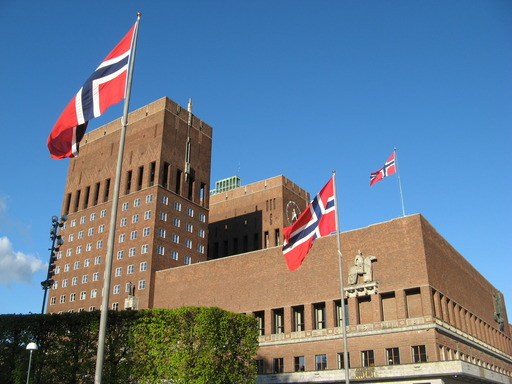
\includegraphics[keepaspectratio,height=7.75em]{NorNet-Configuration-Images/Universitetet_i_Oslo.jpeg}}} & \multicolumn{1}{|l|}{City} & \multicolumn{3}{|l|}{\index{Oslo}Oslo} \\* \cline{5-5}\cline{6-6}\cline{7-7}\cline{8-8}
 \multicolumn{4}{|c|}{} & \multicolumn{1}{|l|}{Province} & \multicolumn{3}{|l|}{\index{Oslo}
\includegraphics[keepaspectratio,height=0.8em]{NorNet-Configuration-Images/NO-Oslo.pdf}Oslo} \\* \cline{5-5}\cline{6-6}\cline{7-7}\cline{8-8}
 \multicolumn{4}{|c|}{} & \multicolumn{1}{|l|}{Country} & \multicolumn{3}{|l|}{\index{NO}\index{Norge}
\includegraphics[keepaspectratio,height=0.8em]{NorNet-Configuration-Images/Flag-NO.pdf}Norge (NO)} \\* \cline{5-5}\cline{6-6}\cline{7-7}\cline{8-8}
 \multicolumn{4}{|c|}{} & \multicolumn{1}{|l|}{GPS/ГЛОНАСС} & \multicolumn{3}{|l|}{59.944°N / 10.719°E / 100.0m} \\* \cline{5-5}\cline{6-6}\cline{7-7}\cline{8-8}
 \multicolumn{4}{|c|}{} & \multicolumn{1}{|l|}{Short Name} & \multicolumn{3}{|l|}{\nomenclature{UiO}{Universitetet i Oslo}\index{UiO|see{Universitetet i Oslo}}UiO} \\* \cline{5-5}\cline{6-6}\cline{7-7}\cline{8-8}
 \multicolumn{4}{|c|}{} & \multicolumn{1}{|l|}{Domain} & \multicolumn{3}{|l|}{\index{uio.nornet}uio.nornet} \\* \cline{5-5}\cline{6-6}\cline{7-7}\cline{8-8}
 \multicolumn{4}{|c|}{} & \multicolumn{1}{|l|}{URL} & \multicolumn{3}{|l|}{\url{http://www.uio.no}} \\ \hline
 \multicolumn{2}{|p{8em}|}{Node} & \multicolumn{2}{|p{8em}|}{Sliver} & \multicolumn{2}{|p{8em}|}{Provider} & IPv4 & IPv6 \\ \hline
\endfirsthead
\hline
 \multicolumn{8}{|c|}{\textbf{Universitetet i Oslo (continued)}} \\ \hline
 \multicolumn{2}{|p{8em}|}{Node} & \multicolumn{2}{|p{8em}|}{Sliver} & \multicolumn{2}{|p{8em}|}{Provider} & IPv4 & IPv6 \\ \hline
\endhead
 \multirow{12}{*}{\tiny{1}} & \multicolumn{3}{|c|}{\multirow{12}{*}{\tiny{tunnelbox}}} & \multicolumn{2}{|c|}{\multirow{4}{*}{\tiny{\href{https://www.uninett.no}{Uninett} (1)}}} & \tiny{129.240.66.74} & \tiny{2001:700:100:279::4} \\* \cline{7-7}\cline{8-8}
  & \multicolumn{3}{|c|}{} & \multicolumn{2}{|c|}{} & \tiny{10.1.2.1} & \tiny{2001:700:4100:102::1} \\* \cline{7-7}\cline{8-8}
  & \multicolumn{3}{|c|}{} & \multicolumn{2}{|c|}{} & Type: & fibre, business \\* \cline{7-7}\cline{8-8}
  & \multicolumn{3}{|c|}{} & \multicolumn{2}{|c|}{} & Down/Up:  & unspecified \\* \cline{5-5}\cline{6-6}\cline{7-7}\cline{8-8}
  & \multicolumn{3}{|c|}{} & \multicolumn{2}{|c|}{\multirow{4}{*}{\tiny{\href{https://www.broadnet.no}{Broadnet} (10)}}} & \tiny{85.252.121.218} & \frownie{} \\* \cline{7-7}\cline{8-8}
  & \multicolumn{3}{|c|}{} & \multicolumn{2}{|c|}{} & \tiny{10.10.2.1} & \tiny{2001:700:4100:a02::1} \\* \cline{7-7}\cline{8-8}
  & \multicolumn{3}{|c|}{} & \multicolumn{2}{|c|}{} & Type: & ADSL, consumer \\* \cline{7-7}\cline{8-8}
  & \multicolumn{3}{|c|}{} & \multicolumn{2}{|c|}{} & Down/Up:  & unspecified \\* \cline{5-5}\cline{6-6}\cline{7-7}\cline{8-8}
  & \multicolumn{3}{|c|}{} & \multicolumn{2}{|c|}{\multirow{4}{*}{\tiny{\href{http://www.powertech.no}{PowerTech} (9)}}} & \tiny{195.159.158.198} & \tiny{2001:840:4abd::4} \\* \cline{7-7}\cline{8-8}
  & \multicolumn{3}{|c|}{} & \multicolumn{2}{|c|}{} & \tiny{10.9.2.1} & \tiny{2001:700:4100:902::1} \\* \cline{7-7}\cline{8-8}
  & \multicolumn{3}{|c|}{} & \multicolumn{2}{|c|}{} & Type: & ADSL, consumer \\* \cline{7-7}\cline{8-8}
  & \multicolumn{3}{|c|}{} & \multicolumn{2}{|c|}{} & Down/Up:  & unspecified \\ \hline
 \multirow{48}{*}{\tiny{100}} & \multicolumn{1}{|l|}{\multirow{48}{*}{\tiny{bjoervika}}} & \multicolumn{2}{|c|}{\multirow{3}{*}{\tiny{Root Context}}} & \multicolumn{2}{|c|}{\tiny{\href{https://www.uninett.no}{Uninett} (1)}} & \tiny{10.1.2.100} & \tiny{2001:700:4100:102::64} \\* \cline{5-5}\cline{6-6}\cline{7-7}\cline{8-8}
  &  & \multicolumn{2}{|c|}{} & \multicolumn{2}{|c|}{\tiny{\href{https://www.broadnet.no}{Broadnet} (10)}} & \tiny{10.10.2.100} & \tiny{2001:700:4100:a02::64} \\* \cline{5-5}\cline{6-6}\cline{7-7}\cline{8-8}
  &  & \multicolumn{2}{|c|}{} & \multicolumn{2}{|c|}{\tiny{\href{http://www.powertech.no}{PowerTech} (9)}} & \tiny{10.9.2.100} & \tiny{2001:700:4100:902::64} \\* \cline{3-3}\cline{4-4}\cline{5-5}\cline{6-6}\cline{7-7}\cline{8-8}
  &  & \multirow{3}{*}{\tiny{117}} & \multicolumn{1}{|l|}{\multirow{3}{*}{\tiny{srl-nndemo}}} & \multicolumn{2}{|c|}{\tiny{\href{https://www.uninett.no}{Uninett} (1)}} & \tiny{10.1.2.117} & \tiny{2001:700:4100:102::75:64} \\* \cline{5-5}\cline{6-6}\cline{7-7}\cline{8-8}
  &  &  &  & \multicolumn{2}{|c|}{\tiny{\href{https://www.broadnet.no}{Broadnet} (10)}} & \tiny{10.10.2.117} & \tiny{2001:700:4100:a02::75:64} \\* \cline{5-5}\cline{6-6}\cline{7-7}\cline{8-8}
  &  &  &  & \multicolumn{2}{|c|}{\tiny{\href{http://www.powertech.no}{PowerTech} (9)}} & \tiny{10.9.2.117} & \tiny{2001:700:4100:902::75:64} \\* \cline{3-3}\cline{4-4}\cline{5-5}\cline{6-6}\cline{7-7}\cline{8-8}
  &  & \multirow{3}{*}{\tiny{119}} & \multicolumn{1}{|l|}{\multirow{3}{*}{\tiny{tuda-sereon}}} & \multicolumn{2}{|c|}{\tiny{\href{https://www.uninett.no}{Uninett} (1)}} & \tiny{10.1.2.119} & \tiny{2001:700:4100:102::77:64} \\* \cline{5-5}\cline{6-6}\cline{7-7}\cline{8-8}
  &  &  &  & \multicolumn{2}{|c|}{\tiny{\href{https://www.broadnet.no}{Broadnet} (10)}} & \tiny{10.10.2.119} & \tiny{2001:700:4100:a02::77:64} \\* \cline{5-5}\cline{6-6}\cline{7-7}\cline{8-8}
  &  &  &  & \multicolumn{2}{|c|}{\tiny{\href{http://www.powertech.no}{PowerTech} (9)}} & \tiny{10.9.2.119} & \tiny{2001:700:4100:902::77:64} \\* \cline{3-3}\cline{4-4}\cline{5-5}\cline{6-6}\cline{7-7}\cline{8-8}
  &  & \multirow{3}{*}{\tiny{122}} & \multicolumn{1}{|l|}{\multirow{3}{*}{\tiny{srl-test}}} & \multicolumn{2}{|c|}{\tiny{\href{https://www.uninett.no}{Uninett} (1)}} & \tiny{10.1.2.122} & \tiny{2001:700:4100:102::7a:64} \\* \cline{5-5}\cline{6-6}\cline{7-7}\cline{8-8}
  &  &  &  & \multicolumn{2}{|c|}{\tiny{\href{https://www.broadnet.no}{Broadnet} (10)}} & \tiny{10.10.2.122} & \tiny{2001:700:4100:a02::7a:64} \\* \cline{5-5}\cline{6-6}\cline{7-7}\cline{8-8}
  &  &  &  & \multicolumn{2}{|c|}{\tiny{\href{http://www.powertech.no}{PowerTech} (9)}} & \tiny{10.9.2.122} & \tiny{2001:700:4100:902::7a:64} \\* \cline{3-3}\cline{4-4}\cline{5-5}\cline{6-6}\cline{7-7}\cline{8-8}
  &  & \multirow{3}{*}{\tiny{128}} & \multicolumn{1}{|l|}{\multirow{3}{*}{\tiny{srl-netperformance}}} & \multicolumn{2}{|c|}{\tiny{\href{https://www.uninett.no}{Uninett} (1)}} & \tiny{10.1.2.128} & \tiny{2001:700:4100:102::80:64} \\* \cline{5-5}\cline{6-6}\cline{7-7}\cline{8-8}
  &  &  &  & \multicolumn{2}{|c|}{\tiny{\href{https://www.broadnet.no}{Broadnet} (10)}} & \tiny{10.10.2.128} & \tiny{2001:700:4100:a02::80:64} \\* \cline{5-5}\cline{6-6}\cline{7-7}\cline{8-8}
  &  &  &  & \multicolumn{2}{|c|}{\tiny{\href{http://www.powertech.no}{PowerTech} (9)}} & \tiny{10.9.2.128} & \tiny{2001:700:4100:902::80:64} \\* \cline{3-3}\cline{4-4}\cline{5-5}\cline{6-6}\cline{7-7}\cline{8-8}
  &  & \multirow{3}{*}{\tiny{134}} & \multicolumn{1}{|l|}{\multirow{3}{*}{\tiny{ude-multipath}}} & \multicolumn{2}{|c|}{\tiny{\href{https://www.uninett.no}{Uninett} (1)}} & \tiny{10.1.2.134} & \tiny{2001:700:4100:102::86:64} \\* \cline{5-5}\cline{6-6}\cline{7-7}\cline{8-8}
  &  &  &  & \multicolumn{2}{|c|}{\tiny{\href{https://www.broadnet.no}{Broadnet} (10)}} & \tiny{10.10.2.134} & \tiny{2001:700:4100:a02::86:64} \\* \cline{5-5}\cline{6-6}\cline{7-7}\cline{8-8}
  &  &  &  & \multicolumn{2}{|c|}{\tiny{\href{http://www.powertech.no}{PowerTech} (9)}} & \tiny{10.9.2.134} & \tiny{2001:700:4100:902::86:64} \\* \cline{3-3}\cline{4-4}\cline{5-5}\cline{6-6}\cline{7-7}\cline{8-8}
  &  & \multirow{3}{*}{\tiny{135}} & \multicolumn{1}{|l|}{\multirow{3}{*}{\tiny{hu-multipath}}} & \multicolumn{2}{|c|}{\tiny{\href{https://www.uninett.no}{Uninett} (1)}} & \tiny{10.1.2.135} & \tiny{2001:700:4100:102::87:64} \\* \cline{5-5}\cline{6-6}\cline{7-7}\cline{8-8}
  &  &  &  & \multicolumn{2}{|c|}{\tiny{\href{https://www.broadnet.no}{Broadnet} (10)}} & \tiny{10.10.2.135} & \tiny{2001:700:4100:a02::87:64} \\* \cline{5-5}\cline{6-6}\cline{7-7}\cline{8-8}
  &  &  &  & \multicolumn{2}{|c|}{\tiny{\href{http://www.powertech.no}{PowerTech} (9)}} & \tiny{10.9.2.135} & \tiny{2001:700:4100:902::87:64} \\* \cline{3-3}\cline{4-4}\cline{5-5}\cline{6-6}\cline{7-7}\cline{8-8}
  &  & \multirow{3}{*}{\tiny{137}} & \multicolumn{1}{|l|}{\multirow{3}{*}{\tiny{hu-jerry}}} & \multicolumn{2}{|c|}{\tiny{\href{https://www.uninett.no}{Uninett} (1)}} & \tiny{10.1.2.137} & \tiny{2001:700:4100:102::89:64} \\* \cline{5-5}\cline{6-6}\cline{7-7}\cline{8-8}
  &  &  &  & \multicolumn{2}{|c|}{\tiny{\href{https://www.broadnet.no}{Broadnet} (10)}} & \tiny{10.10.2.137} & \tiny{2001:700:4100:a02::89:64} \\* \cline{5-5}\cline{6-6}\cline{7-7}\cline{8-8}
  &  &  &  & \multicolumn{2}{|c|}{\tiny{\href{http://www.powertech.no}{PowerTech} (9)}} & \tiny{10.9.2.137} & \tiny{2001:700:4100:902::89:64} \\* \cline{3-3}\cline{4-4}\cline{5-5}\cline{6-6}\cline{7-7}\cline{8-8}
  &  & \multirow{3}{*}{\tiny{140}} & \multicolumn{1}{|l|}{\multirow{3}{*}{\tiny{ntnu-test}}} & \multicolumn{2}{|c|}{\tiny{\href{https://www.uninett.no}{Uninett} (1)}} & \tiny{10.1.2.140} & \tiny{2001:700:4100:102::8c:64} \\* \cline{5-5}\cline{6-6}\cline{7-7}\cline{8-8}
  &  &  &  & \multicolumn{2}{|c|}{\tiny{\href{https://www.broadnet.no}{Broadnet} (10)}} & \tiny{10.10.2.140} & \tiny{2001:700:4100:a02::8c:64} \\* \cline{5-5}\cline{6-6}\cline{7-7}\cline{8-8}
  &  &  &  & \multicolumn{2}{|c|}{\tiny{\href{http://www.powertech.no}{PowerTech} (9)}} & \tiny{10.9.2.140} & \tiny{2001:700:4100:902::8c:64} \\* \cline{3-3}\cline{4-4}\cline{5-5}\cline{6-6}\cline{7-7}\cline{8-8}
  &  & \multirow{3}{*}{\tiny{147}} & \multicolumn{1}{|l|}{\multirow{3}{*}{\tiny{uib-mptcp}}} & \multicolumn{2}{|c|}{\tiny{\href{https://www.uninett.no}{Uninett} (1)}} & \tiny{10.1.2.147} & \tiny{2001:700:4100:102::93:64} \\* \cline{5-5}\cline{6-6}\cline{7-7}\cline{8-8}
  &  &  &  & \multicolumn{2}{|c|}{\tiny{\href{https://www.broadnet.no}{Broadnet} (10)}} & \tiny{10.10.2.147} & \tiny{2001:700:4100:a02::93:64} \\* \cline{5-5}\cline{6-6}\cline{7-7}\cline{8-8}
  &  &  &  & \multicolumn{2}{|c|}{\tiny{\href{http://www.powertech.no}{PowerTech} (9)}} & \tiny{10.9.2.147} & \tiny{2001:700:4100:902::93:64} \\* \cline{3-3}\cline{4-4}\cline{5-5}\cline{6-6}\cline{7-7}\cline{8-8}
  &  & \multirow{3}{*}{\tiny{155}} & \multicolumn{1}{|l|}{\multirow{3}{*}{\tiny{ude-delaytest}}} & \multicolumn{2}{|c|}{\tiny{\href{https://www.uninett.no}{Uninett} (1)}} & \tiny{10.1.2.155} & \tiny{2001:700:4100:102::9b:64} \\* \cline{5-5}\cline{6-6}\cline{7-7}\cline{8-8}
  &  &  &  & \multicolumn{2}{|c|}{\tiny{\href{https://www.broadnet.no}{Broadnet} (10)}} & \tiny{10.10.2.155} & \tiny{2001:700:4100:a02::9b:64} \\* \cline{5-5}\cline{6-6}\cline{7-7}\cline{8-8}
  &  &  &  & \multicolumn{2}{|c|}{\tiny{\href{http://www.powertech.no}{PowerTech} (9)}} & \tiny{10.9.2.155} & \tiny{2001:700:4100:902::9b:64} \\* \cline{3-3}\cline{4-4}\cline{5-5}\cline{6-6}\cline{7-7}\cline{8-8}
  &  & \multirow{3}{*}{\tiny{167}} & \multicolumn{1}{|l|}{\multirow{3}{*}{\tiny{srl-mptcp}}} & \multicolumn{2}{|c|}{\tiny{\href{https://www.uninett.no}{Uninett} (1)}} & \tiny{10.1.2.167} & \tiny{2001:700:4100:102::a7:64} \\* \cline{5-5}\cline{6-6}\cline{7-7}\cline{8-8}
  &  &  &  & \multicolumn{2}{|c|}{\tiny{\href{https://www.broadnet.no}{Broadnet} (10)}} & \tiny{10.10.2.167} & \tiny{2001:700:4100:a02::a7:64} \\* \cline{5-5}\cline{6-6}\cline{7-7}\cline{8-8}
  &  &  &  & \multicolumn{2}{|c|}{\tiny{\href{http://www.powertech.no}{PowerTech} (9)}} & \tiny{10.9.2.167} & \tiny{2001:700:4100:902::a7:64} \\* \cline{3-3}\cline{4-4}\cline{5-5}\cline{6-6}\cline{7-7}\cline{8-8}
  &  & \multirow{3}{*}{\tiny{177}} & \multicolumn{1}{|l|}{\multirow{3}{*}{\tiny{haw-cmt}}} & \multicolumn{2}{|c|}{\tiny{\href{https://www.uninett.no}{Uninett} (1)}} & \tiny{10.1.2.177} & \tiny{2001:700:4100:102::b1:64} \\* \cline{5-5}\cline{6-6}\cline{7-7}\cline{8-8}
  &  &  &  & \multicolumn{2}{|c|}{\tiny{\href{https://www.broadnet.no}{Broadnet} (10)}} & \tiny{10.10.2.177} & \tiny{2001:700:4100:a02::b1:64} \\* \cline{5-5}\cline{6-6}\cline{7-7}\cline{8-8}
  &  &  &  & \multicolumn{2}{|c|}{\tiny{\href{http://www.powertech.no}{PowerTech} (9)}} & \tiny{10.9.2.177} & \tiny{2001:700:4100:902::b1:64} \\* \cline{3-3}\cline{4-4}\cline{5-5}\cline{6-6}\cline{7-7}\cline{8-8}
  &  & \multirow{3}{*}{\tiny{179}} & \multicolumn{1}{|l|}{\multirow{3}{*}{\tiny{hu-zhoufeng}}} & \multicolumn{2}{|c|}{\tiny{\href{https://www.uninett.no}{Uninett} (1)}} & \tiny{10.1.2.179} & \tiny{2001:700:4100:102::b3:64} \\* \cline{5-5}\cline{6-6}\cline{7-7}\cline{8-8}
  &  &  &  & \multicolumn{2}{|c|}{\tiny{\href{https://www.broadnet.no}{Broadnet} (10)}} & \tiny{10.10.2.179} & \tiny{2001:700:4100:a02::b3:64} \\* \cline{5-5}\cline{6-6}\cline{7-7}\cline{8-8}
  &  &  &  & \multicolumn{2}{|c|}{\tiny{\href{http://www.powertech.no}{PowerTech} (9)}} & \tiny{10.9.2.179} & \tiny{2001:700:4100:902::b3:64} \\* \cline{3-3}\cline{4-4}\cline{5-5}\cline{6-6}\cline{7-7}\cline{8-8}
  &  & \multirow{3}{*}{\tiny{189}} & \multicolumn{1}{|l|}{\multirow{3}{*}{\tiny{hu-fufa}}} & \multicolumn{2}{|c|}{\tiny{\href{https://www.uninett.no}{Uninett} (1)}} & \tiny{10.1.2.189} & \tiny{2001:700:4100:102::bd:64} \\* \cline{5-5}\cline{6-6}\cline{7-7}\cline{8-8}
  &  &  &  & \multicolumn{2}{|c|}{\tiny{\href{https://www.broadnet.no}{Broadnet} (10)}} & \tiny{10.10.2.189} & \tiny{2001:700:4100:a02::bd:64} \\* \cline{5-5}\cline{6-6}\cline{7-7}\cline{8-8}
  &  &  &  & \multicolumn{2}{|c|}{\tiny{\href{http://www.powertech.no}{PowerTech} (9)}} & \tiny{10.9.2.189} & \tiny{2001:700:4100:902::bd:64} \\* \cline{3-3}\cline{4-4}\cline{5-5}\cline{6-6}\cline{7-7}\cline{8-8}
  &  & \multirow{3}{*}{\tiny{193}} & \multicolumn{1}{|l|}{\multirow{3}{*}{\tiny{hu-tanqilin}}} & \multicolumn{2}{|c|}{\tiny{\href{https://www.uninett.no}{Uninett} (1)}} & \tiny{10.1.2.193} & \tiny{2001:700:4100:102::c1:64} \\* \cline{5-5}\cline{6-6}\cline{7-7}\cline{8-8}
  &  &  &  & \multicolumn{2}{|c|}{\tiny{\href{https://www.broadnet.no}{Broadnet} (10)}} & \tiny{10.10.2.193} & \tiny{2001:700:4100:a02::c1:64} \\* \cline{5-5}\cline{6-6}\cline{7-7}\cline{8-8}
  &  &  &  & \multicolumn{2}{|c|}{\tiny{\href{http://www.powertech.no}{PowerTech} (9)}} & \tiny{10.9.2.193} & \tiny{2001:700:4100:902::c1:64} \\ \hline
 \multirow{57}{*}{\tiny{101}} & \multicolumn{1}{|l|}{\multirow{57}{*}{\tiny{ekeberg}}} & \multicolumn{2}{|c|}{\multirow{3}{*}{\tiny{Root Context}}} & \multicolumn{2}{|c|}{\tiny{\href{https://www.uninett.no}{Uninett} (1)}} & \tiny{10.1.2.101} & \tiny{2001:700:4100:102::65} \\* \cline{5-5}\cline{6-6}\cline{7-7}\cline{8-8}
  &  & \multicolumn{2}{|c|}{} & \multicolumn{2}{|c|}{\tiny{\href{https://www.broadnet.no}{Broadnet} (10)}} & \tiny{10.10.2.101} & \tiny{2001:700:4100:a02::65} \\* \cline{5-5}\cline{6-6}\cline{7-7}\cline{8-8}
  &  & \multicolumn{2}{|c|}{} & \multicolumn{2}{|c|}{\tiny{\href{http://www.powertech.no}{PowerTech} (9)}} & \tiny{10.9.2.101} & \tiny{2001:700:4100:902::65} \\* \cline{3-3}\cline{4-4}\cline{5-5}\cline{6-6}\cline{7-7}\cline{8-8}
  &  & \multirow{3}{*}{\tiny{116}} & \multicolumn{1}{|l|}{\multirow{3}{*}{\tiny{hu-xingzhou}}} & \multicolumn{2}{|c|}{\tiny{\href{https://www.uninett.no}{Uninett} (1)}} & \tiny{10.1.2.116} & \tiny{2001:700:4100:102::74:65} \\* \cline{5-5}\cline{6-6}\cline{7-7}\cline{8-8}
  &  &  &  & \multicolumn{2}{|c|}{\tiny{\href{https://www.broadnet.no}{Broadnet} (10)}} & \tiny{10.10.2.116} & \tiny{2001:700:4100:a02::74:65} \\* \cline{5-5}\cline{6-6}\cline{7-7}\cline{8-8}
  &  &  &  & \multicolumn{2}{|c|}{\tiny{\href{http://www.powertech.no}{PowerTech} (9)}} & \tiny{10.9.2.116} & \tiny{2001:700:4100:902::74:65} \\* \cline{3-3}\cline{4-4}\cline{5-5}\cline{6-6}\cline{7-7}\cline{8-8}
  &  & \multirow{3}{*}{\tiny{118}} & \multicolumn{1}{|l|}{\multirow{3}{*}{\tiny{tuda-sereon}}} & \multicolumn{2}{|c|}{\tiny{\href{https://www.uninett.no}{Uninett} (1)}} & \tiny{10.1.2.118} & \tiny{2001:700:4100:102::76:65} \\* \cline{5-5}\cline{6-6}\cline{7-7}\cline{8-8}
  &  &  &  & \multicolumn{2}{|c|}{\tiny{\href{https://www.broadnet.no}{Broadnet} (10)}} & \tiny{10.10.2.118} & \tiny{2001:700:4100:a02::76:65} \\* \cline{5-5}\cline{6-6}\cline{7-7}\cline{8-8}
  &  &  &  & \multicolumn{2}{|c|}{\tiny{\href{http://www.powertech.no}{PowerTech} (9)}} & \tiny{10.9.2.118} & \tiny{2001:700:4100:902::76:65} \\* \cline{3-3}\cline{4-4}\cline{5-5}\cline{6-6}\cline{7-7}\cline{8-8}
  &  & \multirow{3}{*}{\tiny{120}} & \multicolumn{1}{|l|}{\multirow{3}{*}{\tiny{srl-test}}} & \multicolumn{2}{|c|}{\tiny{\href{https://www.uninett.no}{Uninett} (1)}} & \tiny{10.1.2.120} & \tiny{2001:700:4100:102::78:65} \\* \cline{5-5}\cline{6-6}\cline{7-7}\cline{8-8}
  &  &  &  & \multicolumn{2}{|c|}{\tiny{\href{https://www.broadnet.no}{Broadnet} (10)}} & \tiny{10.10.2.120} & \tiny{2001:700:4100:a02::78:65} \\* \cline{5-5}\cline{6-6}\cline{7-7}\cline{8-8}
  &  &  &  & \multicolumn{2}{|c|}{\tiny{\href{http://www.powertech.no}{PowerTech} (9)}} & \tiny{10.9.2.120} & \tiny{2001:700:4100:902::78:65} \\* \cline{3-3}\cline{4-4}\cline{5-5}\cline{6-6}\cline{7-7}\cline{8-8}
  &  & \multirow{3}{*}{\tiny{126}} & \multicolumn{1}{|l|}{\multirow{3}{*}{\tiny{kau-multipath}}} & \multicolumn{2}{|c|}{\tiny{\href{https://www.uninett.no}{Uninett} (1)}} & \tiny{10.1.2.126} & \tiny{2001:700:4100:102::7e:65} \\* \cline{5-5}\cline{6-6}\cline{7-7}\cline{8-8}
  &  &  &  & \multicolumn{2}{|c|}{\tiny{\href{https://www.broadnet.no}{Broadnet} (10)}} & \tiny{10.10.2.126} & \tiny{2001:700:4100:a02::7e:65} \\* \cline{5-5}\cline{6-6}\cline{7-7}\cline{8-8}
  &  &  &  & \multicolumn{2}{|c|}{\tiny{\href{http://www.powertech.no}{PowerTech} (9)}} & \tiny{10.9.2.126} & \tiny{2001:700:4100:902::7e:65} \\* \cline{3-3}\cline{4-4}\cline{5-5}\cline{6-6}\cline{7-7}\cline{8-8}
  &  & \multirow{3}{*}{\tiny{127}} & \multicolumn{1}{|l|}{\multirow{3}{*}{\tiny{srl-netperformance}}} & \multicolumn{2}{|c|}{\tiny{\href{https://www.uninett.no}{Uninett} (1)}} & \tiny{10.1.2.127} & \tiny{2001:700:4100:102::7f:65} \\* \cline{5-5}\cline{6-6}\cline{7-7}\cline{8-8}
  &  &  &  & \multicolumn{2}{|c|}{\tiny{\href{https://www.broadnet.no}{Broadnet} (10)}} & \tiny{10.10.2.127} & \tiny{2001:700:4100:a02::7f:65} \\* \cline{5-5}\cline{6-6}\cline{7-7}\cline{8-8}
  &  &  &  & \multicolumn{2}{|c|}{\tiny{\href{http://www.powertech.no}{PowerTech} (9)}} & \tiny{10.9.2.127} & \tiny{2001:700:4100:902::7f:65} \\* \cline{3-3}\cline{4-4}\cline{5-5}\cline{6-6}\cline{7-7}\cline{8-8}
  &  & \multirow{3}{*}{\tiny{129}} & \multicolumn{1}{|l|}{\multirow{3}{*}{\tiny{hu-multipath}}} & \multicolumn{2}{|c|}{\tiny{\href{https://www.uninett.no}{Uninett} (1)}} & \tiny{10.1.2.129} & \tiny{2001:700:4100:102::81:65} \\* \cline{5-5}\cline{6-6}\cline{7-7}\cline{8-8}
  &  &  &  & \multicolumn{2}{|c|}{\tiny{\href{https://www.broadnet.no}{Broadnet} (10)}} & \tiny{10.10.2.129} & \tiny{2001:700:4100:a02::81:65} \\* \cline{5-5}\cline{6-6}\cline{7-7}\cline{8-8}
  &  &  &  & \multicolumn{2}{|c|}{\tiny{\href{http://www.powertech.no}{PowerTech} (9)}} & \tiny{10.9.2.129} & \tiny{2001:700:4100:902::81:65} \\* \cline{3-3}\cline{4-4}\cline{5-5}\cline{6-6}\cline{7-7}\cline{8-8}
  &  & \multirow{3}{*}{\tiny{138}} & \multicolumn{1}{|l|}{\multirow{3}{*}{\tiny{ntnu-test}}} & \multicolumn{2}{|c|}{\tiny{\href{https://www.uninett.no}{Uninett} (1)}} & \tiny{10.1.2.138} & \tiny{2001:700:4100:102::8a:65} \\* \cline{5-5}\cline{6-6}\cline{7-7}\cline{8-8}
  &  &  &  & \multicolumn{2}{|c|}{\tiny{\href{https://www.broadnet.no}{Broadnet} (10)}} & \tiny{10.10.2.138} & \tiny{2001:700:4100:a02::8a:65} \\* \cline{5-5}\cline{6-6}\cline{7-7}\cline{8-8}
  &  &  &  & \multicolumn{2}{|c|}{\tiny{\href{http://www.powertech.no}{PowerTech} (9)}} & \tiny{10.9.2.138} & \tiny{2001:700:4100:902::8a:65} \\* \cline{3-3}\cline{4-4}\cline{5-5}\cline{6-6}\cline{7-7}\cline{8-8}
  &  & \multirow{3}{*}{\tiny{144}} & \multicolumn{1}{|l|}{\multirow{3}{*}{\tiny{srl-nndemo}}} & \multicolumn{2}{|c|}{\tiny{\href{https://www.uninett.no}{Uninett} (1)}} & \tiny{10.1.2.144} & \tiny{2001:700:4100:102::90:65} \\* \cline{5-5}\cline{6-6}\cline{7-7}\cline{8-8}
  &  &  &  & \multicolumn{2}{|c|}{\tiny{\href{https://www.broadnet.no}{Broadnet} (10)}} & \tiny{10.10.2.144} & \tiny{2001:700:4100:a02::90:65} \\* \cline{5-5}\cline{6-6}\cline{7-7}\cline{8-8}
  &  &  &  & \multicolumn{2}{|c|}{\tiny{\href{http://www.powertech.no}{PowerTech} (9)}} & \tiny{10.9.2.144} & \tiny{2001:700:4100:902::90:65} \\* \cline{3-3}\cline{4-4}\cline{5-5}\cline{6-6}\cline{7-7}\cline{8-8}
  &  & \multirow{3}{*}{\tiny{146}} & \multicolumn{1}{|l|}{\multirow{3}{*}{\tiny{uib-mptcp}}} & \multicolumn{2}{|c|}{\tiny{\href{https://www.uninett.no}{Uninett} (1)}} & \tiny{10.1.2.146} & \tiny{2001:700:4100:102::92:65} \\* \cline{5-5}\cline{6-6}\cline{7-7}\cline{8-8}
  &  &  &  & \multicolumn{2}{|c|}{\tiny{\href{https://www.broadnet.no}{Broadnet} (10)}} & \tiny{10.10.2.146} & \tiny{2001:700:4100:a02::92:65} \\* \cline{5-5}\cline{6-6}\cline{7-7}\cline{8-8}
  &  &  &  & \multicolumn{2}{|c|}{\tiny{\href{http://www.powertech.no}{PowerTech} (9)}} & \tiny{10.9.2.146} & \tiny{2001:700:4100:902::92:65} \\* \cline{3-3}\cline{4-4}\cline{5-5}\cline{6-6}\cline{7-7}\cline{8-8}
  &  & \multirow{3}{*}{\tiny{150}} & \multicolumn{1}{|l|}{\multirow{3}{*}{\tiny{srl-mptcp}}} & \multicolumn{2}{|c|}{\tiny{\href{https://www.uninett.no}{Uninett} (1)}} & \tiny{10.1.2.150} & \tiny{2001:700:4100:102::96:65} \\* \cline{5-5}\cline{6-6}\cline{7-7}\cline{8-8}
  &  &  &  & \multicolumn{2}{|c|}{\tiny{\href{https://www.broadnet.no}{Broadnet} (10)}} & \tiny{10.10.2.150} & \tiny{2001:700:4100:a02::96:65} \\* \cline{5-5}\cline{6-6}\cline{7-7}\cline{8-8}
  &  &  &  & \multicolumn{2}{|c|}{\tiny{\href{http://www.powertech.no}{PowerTech} (9)}} & \tiny{10.9.2.150} & \tiny{2001:700:4100:902::96:65} \\* \cline{3-3}\cline{4-4}\cline{5-5}\cline{6-6}\cline{7-7}\cline{8-8}
  &  & \multirow{3}{*}{\tiny{154}} & \multicolumn{1}{|l|}{\multirow{3}{*}{\tiny{ude-delaytest}}} & \multicolumn{2}{|c|}{\tiny{\href{https://www.uninett.no}{Uninett} (1)}} & \tiny{10.1.2.154} & \tiny{2001:700:4100:102::9a:65} \\* \cline{5-5}\cline{6-6}\cline{7-7}\cline{8-8}
  &  &  &  & \multicolumn{2}{|c|}{\tiny{\href{https://www.broadnet.no}{Broadnet} (10)}} & \tiny{10.10.2.154} & \tiny{2001:700:4100:a02::9a:65} \\* \cline{5-5}\cline{6-6}\cline{7-7}\cline{8-8}
  &  &  &  & \multicolumn{2}{|c|}{\tiny{\href{http://www.powertech.no}{PowerTech} (9)}} & \tiny{10.9.2.154} & \tiny{2001:700:4100:902::9a:65} \\* \cline{3-3}\cline{4-4}\cline{5-5}\cline{6-6}\cline{7-7}\cline{8-8}
  &  & \multirow{3}{*}{\tiny{160}} & \multicolumn{1}{|l|}{\multirow{3}{*}{\tiny{kau-mptcpsecurity}}} & \multicolumn{2}{|c|}{\tiny{\href{https://www.uninett.no}{Uninett} (1)}} & \tiny{10.1.2.160} & \tiny{2001:700:4100:102::a0:65} \\* \cline{5-5}\cline{6-6}\cline{7-7}\cline{8-8}
  &  &  &  & \multicolumn{2}{|c|}{\tiny{\href{https://www.broadnet.no}{Broadnet} (10)}} & \tiny{10.10.2.160} & \tiny{2001:700:4100:a02::a0:65} \\* \cline{5-5}\cline{6-6}\cline{7-7}\cline{8-8}
  &  &  &  & \multicolumn{2}{|c|}{\tiny{\href{http://www.powertech.no}{PowerTech} (9)}} & \tiny{10.9.2.160} & \tiny{2001:700:4100:902::a0:65} \\* \cline{3-3}\cline{4-4}\cline{5-5}\cline{6-6}\cline{7-7}\cline{8-8}
  &  & \multirow{3}{*}{\tiny{162}} & \multicolumn{1}{|l|}{\multirow{3}{*}{\tiny{hu-yuyintan}}} & \multicolumn{2}{|c|}{\tiny{\href{https://www.uninett.no}{Uninett} (1)}} & \tiny{10.1.2.162} & \tiny{2001:700:4100:102::a2:65} \\* \cline{5-5}\cline{6-6}\cline{7-7}\cline{8-8}
  &  &  &  & \multicolumn{2}{|c|}{\tiny{\href{https://www.broadnet.no}{Broadnet} (10)}} & \tiny{10.10.2.162} & \tiny{2001:700:4100:a02::a2:65} \\* \cline{5-5}\cline{6-6}\cline{7-7}\cline{8-8}
  &  &  &  & \multicolumn{2}{|c|}{\tiny{\href{http://www.powertech.no}{PowerTech} (9)}} & \tiny{10.9.2.162} & \tiny{2001:700:4100:902::a2:65} \\* \cline{3-3}\cline{4-4}\cline{5-5}\cline{6-6}\cline{7-7}\cline{8-8}
  &  & \multirow{3}{*}{\tiny{172}} & \multicolumn{1}{|l|}{\multirow{3}{*}{\tiny{srl-thuen}}} & \multicolumn{2}{|c|}{\tiny{\href{https://www.uninett.no}{Uninett} (1)}} & \tiny{10.1.2.172} & \tiny{2001:700:4100:102::ac:65} \\* \cline{5-5}\cline{6-6}\cline{7-7}\cline{8-8}
  &  &  &  & \multicolumn{2}{|c|}{\tiny{\href{https://www.broadnet.no}{Broadnet} (10)}} & \tiny{10.10.2.172} & \tiny{2001:700:4100:a02::ac:65} \\* \cline{5-5}\cline{6-6}\cline{7-7}\cline{8-8}
  &  &  &  & \multicolumn{2}{|c|}{\tiny{\href{http://www.powertech.no}{PowerTech} (9)}} & \tiny{10.9.2.172} & \tiny{2001:700:4100:902::ac:65} \\* \cline{3-3}\cline{4-4}\cline{5-5}\cline{6-6}\cline{7-7}\cline{8-8}
  &  & \multirow{3}{*}{\tiny{181}} & \multicolumn{1}{|l|}{\multirow{3}{*}{\tiny{hu-chengxi}}} & \multicolumn{2}{|c|}{\tiny{\href{https://www.uninett.no}{Uninett} (1)}} & \tiny{10.1.2.181} & \tiny{2001:700:4100:102::b5:65} \\* \cline{5-5}\cline{6-6}\cline{7-7}\cline{8-8}
  &  &  &  & \multicolumn{2}{|c|}{\tiny{\href{https://www.broadnet.no}{Broadnet} (10)}} & \tiny{10.10.2.181} & \tiny{2001:700:4100:a02::b5:65} \\* \cline{5-5}\cline{6-6}\cline{7-7}\cline{8-8}
  &  &  &  & \multicolumn{2}{|c|}{\tiny{\href{http://www.powertech.no}{PowerTech} (9)}} & \tiny{10.9.2.181} & \tiny{2001:700:4100:902::b5:65} \\* \cline{3-3}\cline{4-4}\cline{5-5}\cline{6-6}\cline{7-7}\cline{8-8}
  &  & \multirow{3}{*}{\tiny{186}} & \multicolumn{1}{|l|}{\multirow{3}{*}{\tiny{hu-hanbaokuang}}} & \multicolumn{2}{|c|}{\tiny{\href{https://www.uninett.no}{Uninett} (1)}} & \tiny{10.1.2.186} & \tiny{2001:700:4100:102::ba:65} \\* \cline{5-5}\cline{6-6}\cline{7-7}\cline{8-8}
  &  &  &  & \multicolumn{2}{|c|}{\tiny{\href{https://www.broadnet.no}{Broadnet} (10)}} & \tiny{10.10.2.186} & \tiny{2001:700:4100:a02::ba:65} \\* \cline{5-5}\cline{6-6}\cline{7-7}\cline{8-8}
  &  &  &  & \multicolumn{2}{|c|}{\tiny{\href{http://www.powertech.no}{PowerTech} (9)}} & \tiny{10.9.2.186} & \tiny{2001:700:4100:902::ba:65} \\* \cline{3-3}\cline{4-4}\cline{5-5}\cline{6-6}\cline{7-7}\cline{8-8}
  &  & \multirow{3}{*}{\tiny{188}} & \multicolumn{1}{|l|}{\multirow{3}{*}{\tiny{hu-jiangshuihong}}} & \multicolumn{2}{|c|}{\tiny{\href{https://www.uninett.no}{Uninett} (1)}} & \tiny{10.1.2.188} & \tiny{2001:700:4100:102::bc:65} \\* \cline{5-5}\cline{6-6}\cline{7-7}\cline{8-8}
  &  &  &  & \multicolumn{2}{|c|}{\tiny{\href{https://www.broadnet.no}{Broadnet} (10)}} & \tiny{10.10.2.188} & \tiny{2001:700:4100:a02::bc:65} \\* \cline{5-5}\cline{6-6}\cline{7-7}\cline{8-8}
  &  &  &  & \multicolumn{2}{|c|}{\tiny{\href{http://www.powertech.no}{PowerTech} (9)}} & \tiny{10.9.2.188} & \tiny{2001:700:4100:902::bc:65} \\* \cline{3-3}\cline{4-4}\cline{5-5}\cline{6-6}\cline{7-7}\cline{8-8}
  &  & \multirow{3}{*}{\tiny{196}} & \multicolumn{1}{|l|}{\multirow{3}{*}{\tiny{hu-kunwang}}} & \multicolumn{2}{|c|}{\tiny{\href{https://www.uninett.no}{Uninett} (1)}} & \tiny{10.1.2.196} & \tiny{2001:700:4100:102::c4:65} \\* \cline{5-5}\cline{6-6}\cline{7-7}\cline{8-8}
  &  &  &  & \multicolumn{2}{|c|}{\tiny{\href{https://www.broadnet.no}{Broadnet} (10)}} & \tiny{10.10.2.196} & \tiny{2001:700:4100:a02::c4:65} \\* \cline{5-5}\cline{6-6}\cline{7-7}\cline{8-8}
  &  &  &  & \multicolumn{2}{|c|}{\tiny{\href{http://www.powertech.no}{PowerTech} (9)}} & \tiny{10.9.2.196} & \tiny{2001:700:4100:902::c4:65} \\ \hline
 \multirow{42}{*}{\tiny{102}} & \multicolumn{1}{|l|}{\multirow{42}{*}{\tiny{furuset}}} & \multicolumn{2}{|c|}{\multirow{3}{*}{\tiny{Root Context}}} & \multicolumn{2}{|c|}{\tiny{\href{https://www.uninett.no}{Uninett} (1)}} & \tiny{10.1.2.102} & \tiny{2001:700:4100:102::66} \\* \cline{5-5}\cline{6-6}\cline{7-7}\cline{8-8}
  &  & \multicolumn{2}{|c|}{} & \multicolumn{2}{|c|}{\tiny{\href{https://www.broadnet.no}{Broadnet} (10)}} & \tiny{10.10.2.102} & \tiny{2001:700:4100:a02::66} \\* \cline{5-5}\cline{6-6}\cline{7-7}\cline{8-8}
  &  & \multicolumn{2}{|c|}{} & \multicolumn{2}{|c|}{\tiny{\href{http://www.powertech.no}{PowerTech} (9)}} & \tiny{10.9.2.102} & \tiny{2001:700:4100:902::66} \\* \cline{3-3}\cline{4-4}\cline{5-5}\cline{6-6}\cline{7-7}\cline{8-8}
  &  & \multirow{3}{*}{\tiny{123}} & \multicolumn{1}{|l|}{\multirow{3}{*}{\tiny{srl-test}}} & \multicolumn{2}{|c|}{\tiny{\href{https://www.uninett.no}{Uninett} (1)}} & \tiny{10.1.2.123} & \tiny{2001:700:4100:102::7b:66} \\* \cline{5-5}\cline{6-6}\cline{7-7}\cline{8-8}
  &  &  &  & \multicolumn{2}{|c|}{\tiny{\href{https://www.broadnet.no}{Broadnet} (10)}} & \tiny{10.10.2.123} & \tiny{2001:700:4100:a02::7b:66} \\* \cline{5-5}\cline{6-6}\cline{7-7}\cline{8-8}
  &  &  &  & \multicolumn{2}{|c|}{\tiny{\href{http://www.powertech.no}{PowerTech} (9)}} & \tiny{10.9.2.123} & \tiny{2001:700:4100:902::7b:66} \\* \cline{3-3}\cline{4-4}\cline{5-5}\cline{6-6}\cline{7-7}\cline{8-8}
  &  & \multirow{3}{*}{\tiny{130}} & \multicolumn{1}{|l|}{\multirow{3}{*}{\tiny{hu-multipath}}} & \multicolumn{2}{|c|}{\tiny{\href{https://www.uninett.no}{Uninett} (1)}} & \tiny{10.1.2.130} & \tiny{2001:700:4100:102::82:66} \\* \cline{5-5}\cline{6-6}\cline{7-7}\cline{8-8}
  &  &  &  & \multicolumn{2}{|c|}{\tiny{\href{https://www.broadnet.no}{Broadnet} (10)}} & \tiny{10.10.2.130} & \tiny{2001:700:4100:a02::82:66} \\* \cline{5-5}\cline{6-6}\cline{7-7}\cline{8-8}
  &  &  &  & \multicolumn{2}{|c|}{\tiny{\href{http://www.powertech.no}{PowerTech} (9)}} & \tiny{10.9.2.130} & \tiny{2001:700:4100:902::82:66} \\* \cline{3-3}\cline{4-4}\cline{5-5}\cline{6-6}\cline{7-7}\cline{8-8}
  &  & \multirow{3}{*}{\tiny{131}} & \multicolumn{1}{|l|}{\multirow{3}{*}{\tiny{srl-seattle}}} & \multicolumn{2}{|c|}{\tiny{\href{https://www.uninett.no}{Uninett} (1)}} & \tiny{10.1.2.131} & \tiny{2001:700:4100:102::83:66} \\* \cline{5-5}\cline{6-6}\cline{7-7}\cline{8-8}
  &  &  &  & \multicolumn{2}{|c|}{\tiny{\href{https://www.broadnet.no}{Broadnet} (10)}} & \tiny{10.10.2.131} & \tiny{2001:700:4100:a02::83:66} \\* \cline{5-5}\cline{6-6}\cline{7-7}\cline{8-8}
  &  &  &  & \multicolumn{2}{|c|}{\tiny{\href{http://www.powertech.no}{PowerTech} (9)}} & \tiny{10.9.2.131} & \tiny{2001:700:4100:902::83:66} \\* \cline{3-3}\cline{4-4}\cline{5-5}\cline{6-6}\cline{7-7}\cline{8-8}
  &  & \multirow{3}{*}{\tiny{141}} & \multicolumn{1}{|l|}{\multirow{3}{*}{\tiny{ntnu-test}}} & \multicolumn{2}{|c|}{\tiny{\href{https://www.uninett.no}{Uninett} (1)}} & \tiny{10.1.2.141} & \tiny{2001:700:4100:102::8d:66} \\* \cline{5-5}\cline{6-6}\cline{7-7}\cline{8-8}
  &  &  &  & \multicolumn{2}{|c|}{\tiny{\href{https://www.broadnet.no}{Broadnet} (10)}} & \tiny{10.10.2.141} & \tiny{2001:700:4100:a02::8d:66} \\* \cline{5-5}\cline{6-6}\cline{7-7}\cline{8-8}
  &  &  &  & \multicolumn{2}{|c|}{\tiny{\href{http://www.powertech.no}{PowerTech} (9)}} & \tiny{10.9.2.141} & \tiny{2001:700:4100:902::8d:66} \\* \cline{3-3}\cline{4-4}\cline{5-5}\cline{6-6}\cline{7-7}\cline{8-8}
  &  & \multirow{3}{*}{\tiny{157}} & \multicolumn{1}{|l|}{\multirow{3}{*}{\tiny{srl-mptcp}}} & \multicolumn{2}{|c|}{\tiny{\href{https://www.uninett.no}{Uninett} (1)}} & \tiny{10.1.2.157} & \tiny{2001:700:4100:102::9d:66} \\* \cline{5-5}\cline{6-6}\cline{7-7}\cline{8-8}
  &  &  &  & \multicolumn{2}{|c|}{\tiny{\href{https://www.broadnet.no}{Broadnet} (10)}} & \tiny{10.10.2.157} & \tiny{2001:700:4100:a02::9d:66} \\* \cline{5-5}\cline{6-6}\cline{7-7}\cline{8-8}
  &  &  &  & \multicolumn{2}{|c|}{\tiny{\href{http://www.powertech.no}{PowerTech} (9)}} & \tiny{10.9.2.157} & \tiny{2001:700:4100:902::9d:66} \\* \cline{3-3}\cline{4-4}\cline{5-5}\cline{6-6}\cline{7-7}\cline{8-8}
  &  & \multirow{3}{*}{\tiny{165}} & \multicolumn{1}{|l|}{\multirow{3}{*}{\tiny{hu-zhoufeng}}} & \multicolumn{2}{|c|}{\tiny{\href{https://www.uninett.no}{Uninett} (1)}} & \tiny{10.1.2.165} & \tiny{2001:700:4100:102::a5:66} \\* \cline{5-5}\cline{6-6}\cline{7-7}\cline{8-8}
  &  &  &  & \multicolumn{2}{|c|}{\tiny{\href{https://www.broadnet.no}{Broadnet} (10)}} & \tiny{10.10.2.165} & \tiny{2001:700:4100:a02::a5:66} \\* \cline{5-5}\cline{6-6}\cline{7-7}\cline{8-8}
  &  &  &  & \multicolumn{2}{|c|}{\tiny{\href{http://www.powertech.no}{PowerTech} (9)}} & \tiny{10.9.2.165} & \tiny{2001:700:4100:902::a5:66} \\* \cline{3-3}\cline{4-4}\cline{5-5}\cline{6-6}\cline{7-7}\cline{8-8}
  &  & \multirow{3}{*}{\tiny{166}} & \multicolumn{1}{|l|}{\multirow{3}{*}{\tiny{tuda-sereon}}} & \multicolumn{2}{|c|}{\tiny{\href{https://www.uninett.no}{Uninett} (1)}} & \tiny{10.1.2.166} & \tiny{2001:700:4100:102::a6:66} \\* \cline{5-5}\cline{6-6}\cline{7-7}\cline{8-8}
  &  &  &  & \multicolumn{2}{|c|}{\tiny{\href{https://www.broadnet.no}{Broadnet} (10)}} & \tiny{10.10.2.166} & \tiny{2001:700:4100:a02::a6:66} \\* \cline{5-5}\cline{6-6}\cline{7-7}\cline{8-8}
  &  &  &  & \multicolumn{2}{|c|}{\tiny{\href{http://www.powertech.no}{PowerTech} (9)}} & \tiny{10.9.2.166} & \tiny{2001:700:4100:902::a6:66} \\* \cline{3-3}\cline{4-4}\cline{5-5}\cline{6-6}\cline{7-7}\cline{8-8}
  &  & \multirow{3}{*}{\tiny{169}} & \multicolumn{1}{|l|}{\multirow{3}{*}{\tiny{srl-queuing}}} & \multicolumn{2}{|c|}{\tiny{\href{https://www.uninett.no}{Uninett} (1)}} & \tiny{10.1.2.169} & \tiny{2001:700:4100:102::a9:66} \\* \cline{5-5}\cline{6-6}\cline{7-7}\cline{8-8}
  &  &  &  & \multicolumn{2}{|c|}{\tiny{\href{https://www.broadnet.no}{Broadnet} (10)}} & \tiny{10.10.2.169} & \tiny{2001:700:4100:a02::a9:66} \\* \cline{5-5}\cline{6-6}\cline{7-7}\cline{8-8}
  &  &  &  & \multicolumn{2}{|c|}{\tiny{\href{http://www.powertech.no}{PowerTech} (9)}} & \tiny{10.9.2.169} & \tiny{2001:700:4100:902::a9:66} \\* \cline{3-3}\cline{4-4}\cline{5-5}\cline{6-6}\cline{7-7}\cline{8-8}
  &  & \multirow{3}{*}{\tiny{171}} & \multicolumn{1}{|l|}{\multirow{3}{*}{\tiny{haw-cmt}}} & \multicolumn{2}{|c|}{\tiny{\href{https://www.uninett.no}{Uninett} (1)}} & \tiny{10.1.2.171} & \tiny{2001:700:4100:102::ab:66} \\* \cline{5-5}\cline{6-6}\cline{7-7}\cline{8-8}
  &  &  &  & \multicolumn{2}{|c|}{\tiny{\href{https://www.broadnet.no}{Broadnet} (10)}} & \tiny{10.10.2.171} & \tiny{2001:700:4100:a02::ab:66} \\* \cline{5-5}\cline{6-6}\cline{7-7}\cline{8-8}
  &  &  &  & \multicolumn{2}{|c|}{\tiny{\href{http://www.powertech.no}{PowerTech} (9)}} & \tiny{10.9.2.171} & \tiny{2001:700:4100:902::ab:66} \\* \cline{3-3}\cline{4-4}\cline{5-5}\cline{6-6}\cline{7-7}\cline{8-8}
  &  & \multirow{3}{*}{\tiny{173}} & \multicolumn{1}{|l|}{\multirow{3}{*}{\tiny{srl-thuen}}} & \multicolumn{2}{|c|}{\tiny{\href{https://www.uninett.no}{Uninett} (1)}} & \tiny{10.1.2.173} & \tiny{2001:700:4100:102::ad:66} \\* \cline{5-5}\cline{6-6}\cline{7-7}\cline{8-8}
  &  &  &  & \multicolumn{2}{|c|}{\tiny{\href{https://www.broadnet.no}{Broadnet} (10)}} & \tiny{10.10.2.173} & \tiny{2001:700:4100:a02::ad:66} \\* \cline{5-5}\cline{6-6}\cline{7-7}\cline{8-8}
  &  &  &  & \multicolumn{2}{|c|}{\tiny{\href{http://www.powertech.no}{PowerTech} (9)}} & \tiny{10.9.2.173} & \tiny{2001:700:4100:902::ad:66} \\* \cline{3-3}\cline{4-4}\cline{5-5}\cline{6-6}\cline{7-7}\cline{8-8}
  &  & \multirow{3}{*}{\tiny{183}} & \multicolumn{1}{|l|}{\multirow{3}{*}{\tiny{hu-chengxi}}} & \multicolumn{2}{|c|}{\tiny{\href{https://www.uninett.no}{Uninett} (1)}} & \tiny{10.1.2.183} & \tiny{2001:700:4100:102::b7:66} \\* \cline{5-5}\cline{6-6}\cline{7-7}\cline{8-8}
  &  &  &  & \multicolumn{2}{|c|}{\tiny{\href{https://www.broadnet.no}{Broadnet} (10)}} & \tiny{10.10.2.183} & \tiny{2001:700:4100:a02::b7:66} \\* \cline{5-5}\cline{6-6}\cline{7-7}\cline{8-8}
  &  &  &  & \multicolumn{2}{|c|}{\tiny{\href{http://www.powertech.no}{PowerTech} (9)}} & \tiny{10.9.2.183} & \tiny{2001:700:4100:902::b7:66} \\* \cline{3-3}\cline{4-4}\cline{5-5}\cline{6-6}\cline{7-7}\cline{8-8}
  &  & \multirow{3}{*}{\tiny{184}} & \multicolumn{1}{|l|}{\multirow{3}{*}{\tiny{hu-yuyintan}}} & \multicolumn{2}{|c|}{\tiny{\href{https://www.uninett.no}{Uninett} (1)}} & \tiny{10.1.2.184} & \tiny{2001:700:4100:102::b8:66} \\* \cline{5-5}\cline{6-6}\cline{7-7}\cline{8-8}
  &  &  &  & \multicolumn{2}{|c|}{\tiny{\href{https://www.broadnet.no}{Broadnet} (10)}} & \tiny{10.10.2.184} & \tiny{2001:700:4100:a02::b8:66} \\* \cline{5-5}\cline{6-6}\cline{7-7}\cline{8-8}
  &  &  &  & \multicolumn{2}{|c|}{\tiny{\href{http://www.powertech.no}{PowerTech} (9)}} & \tiny{10.9.2.184} & \tiny{2001:700:4100:902::b8:66} \\* \cline{3-3}\cline{4-4}\cline{5-5}\cline{6-6}\cline{7-7}\cline{8-8}
  &  & \multirow{3}{*}{\tiny{195}} & \multicolumn{1}{|l|}{\multirow{3}{*}{\tiny{hu-tanqilin}}} & \multicolumn{2}{|c|}{\tiny{\href{https://www.uninett.no}{Uninett} (1)}} & \tiny{10.1.2.195} & \tiny{2001:700:4100:102::c3:66} \\* \cline{5-5}\cline{6-6}\cline{7-7}\cline{8-8}
  &  &  &  & \multicolumn{2}{|c|}{\tiny{\href{https://www.broadnet.no}{Broadnet} (10)}} & \tiny{10.10.2.195} & \tiny{2001:700:4100:a02::c3:66} \\* \cline{5-5}\cline{6-6}\cline{7-7}\cline{8-8}
  &  &  &  & \multicolumn{2}{|c|}{\tiny{\href{http://www.powertech.no}{PowerTech} (9)}} & \tiny{10.9.2.195} & \tiny{2001:700:4100:902::c3:66} \\ \hline
 \multirow{33}{*}{\tiny{103}} & \multicolumn{1}{|l|}{\multirow{33}{*}{\tiny{grefsen}}} & \multicolumn{2}{|c|}{\multirow{3}{*}{\tiny{Root Context}}} & \multicolumn{2}{|c|}{\tiny{\href{https://www.uninett.no}{Uninett} (1)}} & \tiny{10.1.2.103} & \tiny{2001:700:4100:102::67} \\* \cline{5-5}\cline{6-6}\cline{7-7}\cline{8-8}
  &  & \multicolumn{2}{|c|}{} & \multicolumn{2}{|c|}{\tiny{\href{https://www.broadnet.no}{Broadnet} (10)}} & \tiny{10.10.2.103} & \tiny{2001:700:4100:a02::67} \\* \cline{5-5}\cline{6-6}\cline{7-7}\cline{8-8}
  &  & \multicolumn{2}{|c|}{} & \multicolumn{2}{|c|}{\tiny{\href{http://www.powertech.no}{PowerTech} (9)}} & \tiny{10.9.2.103} & \tiny{2001:700:4100:902::67} \\* \cline{3-3}\cline{4-4}\cline{5-5}\cline{6-6}\cline{7-7}\cline{8-8}
  &  & \multirow{3}{*}{\tiny{124}} & \multicolumn{1}{|l|}{\multirow{3}{*}{\tiny{srl-test}}} & \multicolumn{2}{|c|}{\tiny{\href{https://www.uninett.no}{Uninett} (1)}} & \tiny{10.1.2.124} & \tiny{2001:700:4100:102::7c:67} \\* \cline{5-5}\cline{6-6}\cline{7-7}\cline{8-8}
  &  &  &  & \multicolumn{2}{|c|}{\tiny{\href{https://www.broadnet.no}{Broadnet} (10)}} & \tiny{10.10.2.124} & \tiny{2001:700:4100:a02::7c:67} \\* \cline{5-5}\cline{6-6}\cline{7-7}\cline{8-8}
  &  &  &  & \multicolumn{2}{|c|}{\tiny{\href{http://www.powertech.no}{PowerTech} (9)}} & \tiny{10.9.2.124} & \tiny{2001:700:4100:902::7c:67} \\* \cline{3-3}\cline{4-4}\cline{5-5}\cline{6-6}\cline{7-7}\cline{8-8}
  &  & \multirow{3}{*}{\tiny{132}} & \multicolumn{1}{|l|}{\multirow{3}{*}{\tiny{srl-cps}}} & \multicolumn{2}{|c|}{\tiny{\href{https://www.uninett.no}{Uninett} (1)}} & \tiny{10.1.2.132} & \tiny{2001:700:4100:102::84:67} \\* \cline{5-5}\cline{6-6}\cline{7-7}\cline{8-8}
  &  &  &  & \multicolumn{2}{|c|}{\tiny{\href{https://www.broadnet.no}{Broadnet} (10)}} & \tiny{10.10.2.132} & \tiny{2001:700:4100:a02::84:67} \\* \cline{5-5}\cline{6-6}\cline{7-7}\cline{8-8}
  &  &  &  & \multicolumn{2}{|c|}{\tiny{\href{http://www.powertech.no}{PowerTech} (9)}} & \tiny{10.9.2.132} & \tiny{2001:700:4100:902::84:67} \\* \cline{3-3}\cline{4-4}\cline{5-5}\cline{6-6}\cline{7-7}\cline{8-8}
  &  & \multirow{3}{*}{\tiny{142}} & \multicolumn{1}{|l|}{\multirow{3}{*}{\tiny{ntnu-test}}} & \multicolumn{2}{|c|}{\tiny{\href{https://www.uninett.no}{Uninett} (1)}} & \tiny{10.1.2.142} & \tiny{2001:700:4100:102::8e:67} \\* \cline{5-5}\cline{6-6}\cline{7-7}\cline{8-8}
  &  &  &  & \multicolumn{2}{|c|}{\tiny{\href{https://www.broadnet.no}{Broadnet} (10)}} & \tiny{10.10.2.142} & \tiny{2001:700:4100:a02::8e:67} \\* \cline{5-5}\cline{6-6}\cline{7-7}\cline{8-8}
  &  &  &  & \multicolumn{2}{|c|}{\tiny{\href{http://www.powertech.no}{PowerTech} (9)}} & \tiny{10.9.2.142} & \tiny{2001:700:4100:902::8e:67} \\* \cline{3-3}\cline{4-4}\cline{5-5}\cline{6-6}\cline{7-7}\cline{8-8}
  &  & \multirow{3}{*}{\tiny{145}} & \multicolumn{1}{|l|}{\multirow{3}{*}{\tiny{ude-multipath}}} & \multicolumn{2}{|c|}{\tiny{\href{https://www.uninett.no}{Uninett} (1)}} & \tiny{10.1.2.145} & \tiny{2001:700:4100:102::91:67} \\* \cline{5-5}\cline{6-6}\cline{7-7}\cline{8-8}
  &  &  &  & \multicolumn{2}{|c|}{\tiny{\href{https://www.broadnet.no}{Broadnet} (10)}} & \tiny{10.10.2.145} & \tiny{2001:700:4100:a02::91:67} \\* \cline{5-5}\cline{6-6}\cline{7-7}\cline{8-8}
  &  &  &  & \multicolumn{2}{|c|}{\tiny{\href{http://www.powertech.no}{PowerTech} (9)}} & \tiny{10.9.2.145} & \tiny{2001:700:4100:902::91:67} \\* \cline{3-3}\cline{4-4}\cline{5-5}\cline{6-6}\cline{7-7}\cline{8-8}
  &  & \multirow{3}{*}{\tiny{148}} & \multicolumn{1}{|l|}{\multirow{3}{*}{\tiny{hu-multipath}}} & \multicolumn{2}{|c|}{\tiny{\href{https://www.uninett.no}{Uninett} (1)}} & \tiny{10.1.2.148} & \tiny{2001:700:4100:102::94:67} \\* \cline{5-5}\cline{6-6}\cline{7-7}\cline{8-8}
  &  &  &  & \multicolumn{2}{|c|}{\tiny{\href{https://www.broadnet.no}{Broadnet} (10)}} & \tiny{10.10.2.148} & \tiny{2001:700:4100:a02::94:67} \\* \cline{5-5}\cline{6-6}\cline{7-7}\cline{8-8}
  &  &  &  & \multicolumn{2}{|c|}{\tiny{\href{http://www.powertech.no}{PowerTech} (9)}} & \tiny{10.9.2.148} & \tiny{2001:700:4100:902::94:67} \\* \cline{3-3}\cline{4-4}\cline{5-5}\cline{6-6}\cline{7-7}\cline{8-8}
  &  & \multirow{3}{*}{\tiny{156}} & \multicolumn{1}{|l|}{\multirow{3}{*}{\tiny{tuda-sereon}}} & \multicolumn{2}{|c|}{\tiny{\href{https://www.uninett.no}{Uninett} (1)}} & \tiny{10.1.2.156} & \tiny{2001:700:4100:102::9c:67} \\* \cline{5-5}\cline{6-6}\cline{7-7}\cline{8-8}
  &  &  &  & \multicolumn{2}{|c|}{\tiny{\href{https://www.broadnet.no}{Broadnet} (10)}} & \tiny{10.10.2.156} & \tiny{2001:700:4100:a02::9c:67} \\* \cline{5-5}\cline{6-6}\cline{7-7}\cline{8-8}
  &  &  &  & \multicolumn{2}{|c|}{\tiny{\href{http://www.powertech.no}{PowerTech} (9)}} & \tiny{10.9.2.156} & \tiny{2001:700:4100:902::9c:67} \\* \cline{3-3}\cline{4-4}\cline{5-5}\cline{6-6}\cline{7-7}\cline{8-8}
  &  & \multirow{3}{*}{\tiny{164}} & \multicolumn{1}{|l|}{\multirow{3}{*}{\tiny{hu-zhoufeng}}} & \multicolumn{2}{|c|}{\tiny{\href{https://www.uninett.no}{Uninett} (1)}} & \tiny{10.1.2.164} & \tiny{2001:700:4100:102::a4:67} \\* \cline{5-5}\cline{6-6}\cline{7-7}\cline{8-8}
  &  &  &  & \multicolumn{2}{|c|}{\tiny{\href{https://www.broadnet.no}{Broadnet} (10)}} & \tiny{10.10.2.164} & \tiny{2001:700:4100:a02::a4:67} \\* \cline{5-5}\cline{6-6}\cline{7-7}\cline{8-8}
  &  &  &  & \multicolumn{2}{|c|}{\tiny{\href{http://www.powertech.no}{PowerTech} (9)}} & \tiny{10.9.2.164} & \tiny{2001:700:4100:902::a4:67} \\* \cline{3-3}\cline{4-4}\cline{5-5}\cline{6-6}\cline{7-7}\cline{8-8}
  &  & \multirow{3}{*}{\tiny{170}} & \multicolumn{1}{|l|}{\multirow{3}{*}{\tiny{haw-cmt}}} & \multicolumn{2}{|c|}{\tiny{\href{https://www.uninett.no}{Uninett} (1)}} & \tiny{10.1.2.170} & \tiny{2001:700:4100:102::aa:67} \\* \cline{5-5}\cline{6-6}\cline{7-7}\cline{8-8}
  &  &  &  & \multicolumn{2}{|c|}{\tiny{\href{https://www.broadnet.no}{Broadnet} (10)}} & \tiny{10.10.2.170} & \tiny{2001:700:4100:a02::aa:67} \\* \cline{5-5}\cline{6-6}\cline{7-7}\cline{8-8}
  &  &  &  & \multicolumn{2}{|c|}{\tiny{\href{http://www.powertech.no}{PowerTech} (9)}} & \tiny{10.9.2.170} & \tiny{2001:700:4100:902::aa:67} \\* \cline{3-3}\cline{4-4}\cline{5-5}\cline{6-6}\cline{7-7}\cline{8-8}
  &  & \multirow{3}{*}{\tiny{182}} & \multicolumn{1}{|l|}{\multirow{3}{*}{\tiny{hu-xingzhou}}} & \multicolumn{2}{|c|}{\tiny{\href{https://www.uninett.no}{Uninett} (1)}} & \tiny{10.1.2.182} & \tiny{2001:700:4100:102::b6:67} \\* \cline{5-5}\cline{6-6}\cline{7-7}\cline{8-8}
  &  &  &  & \multicolumn{2}{|c|}{\tiny{\href{https://www.broadnet.no}{Broadnet} (10)}} & \tiny{10.10.2.182} & \tiny{2001:700:4100:a02::b6:67} \\* \cline{5-5}\cline{6-6}\cline{7-7}\cline{8-8}
  &  &  &  & \multicolumn{2}{|c|}{\tiny{\href{http://www.powertech.no}{PowerTech} (9)}} & \tiny{10.9.2.182} & \tiny{2001:700:4100:902::b6:67} \\* \cline{3-3}\cline{4-4}\cline{5-5}\cline{6-6}\cline{7-7}\cline{8-8}
  &  & \multirow{3}{*}{\tiny{198}} & \multicolumn{1}{|l|}{\multirow{3}{*}{\tiny{hu-kunwang}}} & \multicolumn{2}{|c|}{\tiny{\href{https://www.uninett.no}{Uninett} (1)}} & \tiny{10.1.2.198} & \tiny{2001:700:4100:102::c6:67} \\* \cline{5-5}\cline{6-6}\cline{7-7}\cline{8-8}
  &  &  &  & \multicolumn{2}{|c|}{\tiny{\href{https://www.broadnet.no}{Broadnet} (10)}} & \tiny{10.10.2.198} & \tiny{2001:700:4100:a02::c6:67} \\* \cline{5-5}\cline{6-6}\cline{7-7}\cline{8-8}
  &  &  &  & \multicolumn{2}{|c|}{\tiny{\href{http://www.powertech.no}{PowerTech} (9)}} & \tiny{10.9.2.198} & \tiny{2001:700:4100:902::c6:67} \\ \hline
 \multirow{36}{*}{\tiny{104}} & \multicolumn{1}{|l|}{\multirow{36}{*}{\tiny{helsfyr}}} & \multicolumn{2}{|c|}{\multirow{3}{*}{\tiny{Root Context}}} & \multicolumn{2}{|c|}{\tiny{\href{https://www.uninett.no}{Uninett} (1)}} & \tiny{10.1.2.104} & \tiny{2001:700:4100:102::68} \\* \cline{5-5}\cline{6-6}\cline{7-7}\cline{8-8}
  &  & \multicolumn{2}{|c|}{} & \multicolumn{2}{|c|}{\tiny{\href{https://www.broadnet.no}{Broadnet} (10)}} & \tiny{10.10.2.104} & \tiny{2001:700:4100:a02::68} \\* \cline{5-5}\cline{6-6}\cline{7-7}\cline{8-8}
  &  & \multicolumn{2}{|c|}{} & \multicolumn{2}{|c|}{\tiny{\href{http://www.powertech.no}{PowerTech} (9)}} & \tiny{10.9.2.104} & \tiny{2001:700:4100:902::68} \\* \cline{3-3}\cline{4-4}\cline{5-5}\cline{6-6}\cline{7-7}\cline{8-8}
  &  & \multirow{3}{*}{\tiny{115}} & \multicolumn{1}{|l|}{\multirow{3}{*}{\tiny{srl-mptcp}}} & \multicolumn{2}{|c|}{\tiny{\href{https://www.uninett.no}{Uninett} (1)}} & \tiny{10.1.2.115} & \tiny{2001:700:4100:102::73:68} \\* \cline{5-5}\cline{6-6}\cline{7-7}\cline{8-8}
  &  &  &  & \multicolumn{2}{|c|}{\tiny{\href{https://www.broadnet.no}{Broadnet} (10)}} & \tiny{10.10.2.115} & \tiny{2001:700:4100:a02::73:68} \\* \cline{5-5}\cline{6-6}\cline{7-7}\cline{8-8}
  &  &  &  & \multicolumn{2}{|c|}{\tiny{\href{http://www.powertech.no}{PowerTech} (9)}} & \tiny{10.9.2.115} & \tiny{2001:700:4100:902::73:68} \\* \cline{3-3}\cline{4-4}\cline{5-5}\cline{6-6}\cline{7-7}\cline{8-8}
  &  & \multirow{3}{*}{\tiny{121}} & \multicolumn{1}{|l|}{\multirow{3}{*}{\tiny{srl-test}}} & \multicolumn{2}{|c|}{\tiny{\href{https://www.uninett.no}{Uninett} (1)}} & \tiny{10.1.2.121} & \tiny{2001:700:4100:102::79:68} \\* \cline{5-5}\cline{6-6}\cline{7-7}\cline{8-8}
  &  &  &  & \multicolumn{2}{|c|}{\tiny{\href{https://www.broadnet.no}{Broadnet} (10)}} & \tiny{10.10.2.121} & \tiny{2001:700:4100:a02::79:68} \\* \cline{5-5}\cline{6-6}\cline{7-7}\cline{8-8}
  &  &  &  & \multicolumn{2}{|c|}{\tiny{\href{http://www.powertech.no}{PowerTech} (9)}} & \tiny{10.9.2.121} & \tiny{2001:700:4100:902::79:68} \\* \cline{3-3}\cline{4-4}\cline{5-5}\cline{6-6}\cline{7-7}\cline{8-8}
  &  & \multirow{3}{*}{\tiny{136}} & \multicolumn{1}{|l|}{\multirow{3}{*}{\tiny{srl-cps}}} & \multicolumn{2}{|c|}{\tiny{\href{https://www.uninett.no}{Uninett} (1)}} & \tiny{10.1.2.136} & \tiny{2001:700:4100:102::88:68} \\* \cline{5-5}\cline{6-6}\cline{7-7}\cline{8-8}
  &  &  &  & \multicolumn{2}{|c|}{\tiny{\href{https://www.broadnet.no}{Broadnet} (10)}} & \tiny{10.10.2.136} & \tiny{2001:700:4100:a02::88:68} \\* \cline{5-5}\cline{6-6}\cline{7-7}\cline{8-8}
  &  &  &  & \multicolumn{2}{|c|}{\tiny{\href{http://www.powertech.no}{PowerTech} (9)}} & \tiny{10.9.2.136} & \tiny{2001:700:4100:902::88:68} \\* \cline{3-3}\cline{4-4}\cline{5-5}\cline{6-6}\cline{7-7}\cline{8-8}
  &  & \multirow{3}{*}{\tiny{139}} & \multicolumn{1}{|l|}{\multirow{3}{*}{\tiny{ntnu-test}}} & \multicolumn{2}{|c|}{\tiny{\href{https://www.uninett.no}{Uninett} (1)}} & \tiny{10.1.2.139} & \tiny{2001:700:4100:102::8b:68} \\* \cline{5-5}\cline{6-6}\cline{7-7}\cline{8-8}
  &  &  &  & \multicolumn{2}{|c|}{\tiny{\href{https://www.broadnet.no}{Broadnet} (10)}} & \tiny{10.10.2.139} & \tiny{2001:700:4100:a02::8b:68} \\* \cline{5-5}\cline{6-6}\cline{7-7}\cline{8-8}
  &  &  &  & \multicolumn{2}{|c|}{\tiny{\href{http://www.powertech.no}{PowerTech} (9)}} & \tiny{10.9.2.139} & \tiny{2001:700:4100:902::8b:68} \\* \cline{3-3}\cline{4-4}\cline{5-5}\cline{6-6}\cline{7-7}\cline{8-8}
  &  & \multirow{3}{*}{\tiny{149}} & \multicolumn{1}{|l|}{\multirow{3}{*}{\tiny{hu-multipath}}} & \multicolumn{2}{|c|}{\tiny{\href{https://www.uninett.no}{Uninett} (1)}} & \tiny{10.1.2.149} & \tiny{2001:700:4100:102::95:68} \\* \cline{5-5}\cline{6-6}\cline{7-7}\cline{8-8}
  &  &  &  & \multicolumn{2}{|c|}{\tiny{\href{https://www.broadnet.no}{Broadnet} (10)}} & \tiny{10.10.2.149} & \tiny{2001:700:4100:a02::95:68} \\* \cline{5-5}\cline{6-6}\cline{7-7}\cline{8-8}
  &  &  &  & \multicolumn{2}{|c|}{\tiny{\href{http://www.powertech.no}{PowerTech} (9)}} & \tiny{10.9.2.149} & \tiny{2001:700:4100:902::95:68} \\* \cline{3-3}\cline{4-4}\cline{5-5}\cline{6-6}\cline{7-7}\cline{8-8}
  &  & \multirow{3}{*}{\tiny{159}} & \multicolumn{1}{|l|}{\multirow{3}{*}{\tiny{tuda-sereon}}} & \multicolumn{2}{|c|}{\tiny{\href{https://www.uninett.no}{Uninett} (1)}} & \tiny{10.1.2.159} & \tiny{2001:700:4100:102::9f:68} \\* \cline{5-5}\cline{6-6}\cline{7-7}\cline{8-8}
  &  &  &  & \multicolumn{2}{|c|}{\tiny{\href{https://www.broadnet.no}{Broadnet} (10)}} & \tiny{10.10.2.159} & \tiny{2001:700:4100:a02::9f:68} \\* \cline{5-5}\cline{6-6}\cline{7-7}\cline{8-8}
  &  &  &  & \multicolumn{2}{|c|}{\tiny{\href{http://www.powertech.no}{PowerTech} (9)}} & \tiny{10.9.2.159} & \tiny{2001:700:4100:902::9f:68} \\* \cline{3-3}\cline{4-4}\cline{5-5}\cline{6-6}\cline{7-7}\cline{8-8}
  &  & \multirow{3}{*}{\tiny{161}} & \multicolumn{1}{|l|}{\multirow{3}{*}{\tiny{kau-mptcpsecurity}}} & \multicolumn{2}{|c|}{\tiny{\href{https://www.uninett.no}{Uninett} (1)}} & \tiny{10.1.2.161} & \tiny{2001:700:4100:102::a1:68} \\* \cline{5-5}\cline{6-6}\cline{7-7}\cline{8-8}
  &  &  &  & \multicolumn{2}{|c|}{\tiny{\href{https://www.broadnet.no}{Broadnet} (10)}} & \tiny{10.10.2.161} & \tiny{2001:700:4100:a02::a1:68} \\* \cline{5-5}\cline{6-6}\cline{7-7}\cline{8-8}
  &  &  &  & \multicolumn{2}{|c|}{\tiny{\href{http://www.powertech.no}{PowerTech} (9)}} & \tiny{10.9.2.161} & \tiny{2001:700:4100:902::a1:68} \\* \cline{3-3}\cline{4-4}\cline{5-5}\cline{6-6}\cline{7-7}\cline{8-8}
  &  & \multirow{3}{*}{\tiny{175}} & \multicolumn{1}{|l|}{\multirow{3}{*}{\tiny{srl-thuen}}} & \multicolumn{2}{|c|}{\tiny{\href{https://www.uninett.no}{Uninett} (1)}} & \tiny{10.1.2.175} & \tiny{2001:700:4100:102::af:68} \\* \cline{5-5}\cline{6-6}\cline{7-7}\cline{8-8}
  &  &  &  & \multicolumn{2}{|c|}{\tiny{\href{https://www.broadnet.no}{Broadnet} (10)}} & \tiny{10.10.2.175} & \tiny{2001:700:4100:a02::af:68} \\* \cline{5-5}\cline{6-6}\cline{7-7}\cline{8-8}
  &  &  &  & \multicolumn{2}{|c|}{\tiny{\href{http://www.powertech.no}{PowerTech} (9)}} & \tiny{10.9.2.175} & \tiny{2001:700:4100:902::af:68} \\* \cline{3-3}\cline{4-4}\cline{5-5}\cline{6-6}\cline{7-7}\cline{8-8}
  &  & \multirow{3}{*}{\tiny{180}} & \multicolumn{1}{|l|}{\multirow{3}{*}{\tiny{kau-multipath}}} & \multicolumn{2}{|c|}{\tiny{\href{https://www.uninett.no}{Uninett} (1)}} & \tiny{10.1.2.180} & \tiny{2001:700:4100:102::b4:68} \\* \cline{5-5}\cline{6-6}\cline{7-7}\cline{8-8}
  &  &  &  & \multicolumn{2}{|c|}{\tiny{\href{https://www.broadnet.no}{Broadnet} (10)}} & \tiny{10.10.2.180} & \tiny{2001:700:4100:a02::b4:68} \\* \cline{5-5}\cline{6-6}\cline{7-7}\cline{8-8}
  &  &  &  & \multicolumn{2}{|c|}{\tiny{\href{http://www.powertech.no}{PowerTech} (9)}} & \tiny{10.9.2.180} & \tiny{2001:700:4100:902::b4:68} \\* \cline{3-3}\cline{4-4}\cline{5-5}\cline{6-6}\cline{7-7}\cline{8-8}
  &  & \multirow{3}{*}{\tiny{187}} & \multicolumn{1}{|l|}{\multirow{3}{*}{\tiny{hu-hanbaokuang}}} & \multicolumn{2}{|c|}{\tiny{\href{https://www.uninett.no}{Uninett} (1)}} & \tiny{10.1.2.187} & \tiny{2001:700:4100:102::bb:68} \\* \cline{5-5}\cline{6-6}\cline{7-7}\cline{8-8}
  &  &  &  & \multicolumn{2}{|c|}{\tiny{\href{https://www.broadnet.no}{Broadnet} (10)}} & \tiny{10.10.2.187} & \tiny{2001:700:4100:a02::bb:68} \\* \cline{5-5}\cline{6-6}\cline{7-7}\cline{8-8}
  &  &  &  & \multicolumn{2}{|c|}{\tiny{\href{http://www.powertech.no}{PowerTech} (9)}} & \tiny{10.9.2.187} & \tiny{2001:700:4100:902::bb:68} \\* \cline{3-3}\cline{4-4}\cline{5-5}\cline{6-6}\cline{7-7}\cline{8-8}
  &  & \multirow{3}{*}{\tiny{191}} & \multicolumn{1}{|l|}{\multirow{3}{*}{\tiny{hu-jiangshuihong}}} & \multicolumn{2}{|c|}{\tiny{\href{https://www.uninett.no}{Uninett} (1)}} & \tiny{10.1.2.191} & \tiny{2001:700:4100:102::bf:68} \\* \cline{5-5}\cline{6-6}\cline{7-7}\cline{8-8}
  &  &  &  & \multicolumn{2}{|c|}{\tiny{\href{https://www.broadnet.no}{Broadnet} (10)}} & \tiny{10.10.2.191} & \tiny{2001:700:4100:a02::bf:68} \\* \cline{5-5}\cline{6-6}\cline{7-7}\cline{8-8}
  &  &  &  & \multicolumn{2}{|c|}{\tiny{\href{http://www.powertech.no}{PowerTech} (9)}} & \tiny{10.9.2.191} & \tiny{2001:700:4100:902::bf:68} \\ \hline
 \multirow{33}{*}{\tiny{105}} & \multicolumn{1}{|l|}{\multirow{33}{*}{\tiny{toeyen}}} & \multicolumn{2}{|c|}{\multirow{3}{*}{\tiny{Root Context}}} & \multicolumn{2}{|c|}{\tiny{\href{https://www.uninett.no}{Uninett} (1)}} & \tiny{10.1.2.105} & \tiny{2001:700:4100:102::69} \\* \cline{5-5}\cline{6-6}\cline{7-7}\cline{8-8}
  &  & \multicolumn{2}{|c|}{} & \multicolumn{2}{|c|}{\tiny{\href{https://www.broadnet.no}{Broadnet} (10)}} & \tiny{10.10.2.105} & \tiny{2001:700:4100:a02::69} \\* \cline{5-5}\cline{6-6}\cline{7-7}\cline{8-8}
  &  & \multicolumn{2}{|c|}{} & \multicolumn{2}{|c|}{\tiny{\href{http://www.powertech.no}{PowerTech} (9)}} & \tiny{10.9.2.105} & \tiny{2001:700:4100:902::69} \\* \cline{3-3}\cline{4-4}\cline{5-5}\cline{6-6}\cline{7-7}\cline{8-8}
  &  & \multirow{3}{*}{\tiny{125}} & \multicolumn{1}{|l|}{\multirow{3}{*}{\tiny{srl-test}}} & \multicolumn{2}{|c|}{\tiny{\href{https://www.uninett.no}{Uninett} (1)}} & \tiny{10.1.2.125} & \tiny{2001:700:4100:102::7d:69} \\* \cline{5-5}\cline{6-6}\cline{7-7}\cline{8-8}
  &  &  &  & \multicolumn{2}{|c|}{\tiny{\href{https://www.broadnet.no}{Broadnet} (10)}} & \tiny{10.10.2.125} & \tiny{2001:700:4100:a02::7d:69} \\* \cline{5-5}\cline{6-6}\cline{7-7}\cline{8-8}
  &  &  &  & \multicolumn{2}{|c|}{\tiny{\href{http://www.powertech.no}{PowerTech} (9)}} & \tiny{10.9.2.125} & \tiny{2001:700:4100:902::7d:69} \\* \cline{3-3}\cline{4-4}\cline{5-5}\cline{6-6}\cline{7-7}\cline{8-8}
  &  & \multirow{3}{*}{\tiny{133}} & \multicolumn{1}{|l|}{\multirow{3}{*}{\tiny{hu-multipath}}} & \multicolumn{2}{|c|}{\tiny{\href{https://www.uninett.no}{Uninett} (1)}} & \tiny{10.1.2.133} & \tiny{2001:700:4100:102::85:69} \\* \cline{5-5}\cline{6-6}\cline{7-7}\cline{8-8}
  &  &  &  & \multicolumn{2}{|c|}{\tiny{\href{https://www.broadnet.no}{Broadnet} (10)}} & \tiny{10.10.2.133} & \tiny{2001:700:4100:a02::85:69} \\* \cline{5-5}\cline{6-6}\cline{7-7}\cline{8-8}
  &  &  &  & \multicolumn{2}{|c|}{\tiny{\href{http://www.powertech.no}{PowerTech} (9)}} & \tiny{10.9.2.133} & \tiny{2001:700:4100:902::85:69} \\* \cline{3-3}\cline{4-4}\cline{5-5}\cline{6-6}\cline{7-7}\cline{8-8}
  &  & \multirow{3}{*}{\tiny{143}} & \multicolumn{1}{|l|}{\multirow{3}{*}{\tiny{ntnu-test}}} & \multicolumn{2}{|c|}{\tiny{\href{https://www.uninett.no}{Uninett} (1)}} & \tiny{10.1.2.143} & \tiny{2001:700:4100:102::8f:69} \\* \cline{5-5}\cline{6-6}\cline{7-7}\cline{8-8}
  &  &  &  & \multicolumn{2}{|c|}{\tiny{\href{https://www.broadnet.no}{Broadnet} (10)}} & \tiny{10.10.2.143} & \tiny{2001:700:4100:a02::8f:69} \\* \cline{5-5}\cline{6-6}\cline{7-7}\cline{8-8}
  &  &  &  & \multicolumn{2}{|c|}{\tiny{\href{http://www.powertech.no}{PowerTech} (9)}} & \tiny{10.9.2.143} & \tiny{2001:700:4100:902::8f:69} \\* \cline{3-3}\cline{4-4}\cline{5-5}\cline{6-6}\cline{7-7}\cline{8-8}
  &  & \multirow{3}{*}{\tiny{158}} & \multicolumn{1}{|l|}{\multirow{3}{*}{\tiny{srl-seattle}}} & \multicolumn{2}{|c|}{\tiny{\href{https://www.uninett.no}{Uninett} (1)}} & \tiny{10.1.2.158} & \tiny{2001:700:4100:102::9e:69} \\* \cline{5-5}\cline{6-6}\cline{7-7}\cline{8-8}
  &  &  &  & \multicolumn{2}{|c|}{\tiny{\href{https://www.broadnet.no}{Broadnet} (10)}} & \tiny{10.10.2.158} & \tiny{2001:700:4100:a02::9e:69} \\* \cline{5-5}\cline{6-6}\cline{7-7}\cline{8-8}
  &  &  &  & \multicolumn{2}{|c|}{\tiny{\href{http://www.powertech.no}{PowerTech} (9)}} & \tiny{10.9.2.158} & \tiny{2001:700:4100:902::9e:69} \\* \cline{3-3}\cline{4-4}\cline{5-5}\cline{6-6}\cline{7-7}\cline{8-8}
  &  & \multirow{3}{*}{\tiny{163}} & \multicolumn{1}{|l|}{\multirow{3}{*}{\tiny{tuda-sereon}}} & \multicolumn{2}{|c|}{\tiny{\href{https://www.uninett.no}{Uninett} (1)}} & \tiny{10.1.2.163} & \tiny{2001:700:4100:102::a3:69} \\* \cline{5-5}\cline{6-6}\cline{7-7}\cline{8-8}
  &  &  &  & \multicolumn{2}{|c|}{\tiny{\href{https://www.broadnet.no}{Broadnet} (10)}} & \tiny{10.10.2.163} & \tiny{2001:700:4100:a02::a3:69} \\* \cline{5-5}\cline{6-6}\cline{7-7}\cline{8-8}
  &  &  &  & \multicolumn{2}{|c|}{\tiny{\href{http://www.powertech.no}{PowerTech} (9)}} & \tiny{10.9.2.163} & \tiny{2001:700:4100:902::a3:69} \\* \cline{3-3}\cline{4-4}\cline{5-5}\cline{6-6}\cline{7-7}\cline{8-8}
  &  & \multirow{3}{*}{\tiny{168}} & \multicolumn{1}{|l|}{\multirow{3}{*}{\tiny{srl-queuing}}} & \multicolumn{2}{|c|}{\tiny{\href{https://www.uninett.no}{Uninett} (1)}} & \tiny{10.1.2.168} & \tiny{2001:700:4100:102::a8:69} \\* \cline{5-5}\cline{6-6}\cline{7-7}\cline{8-8}
  &  &  &  & \multicolumn{2}{|c|}{\tiny{\href{https://www.broadnet.no}{Broadnet} (10)}} & \tiny{10.10.2.168} & \tiny{2001:700:4100:a02::a8:69} \\* \cline{5-5}\cline{6-6}\cline{7-7}\cline{8-8}
  &  &  &  & \multicolumn{2}{|c|}{\tiny{\href{http://www.powertech.no}{PowerTech} (9)}} & \tiny{10.9.2.168} & \tiny{2001:700:4100:902::a8:69} \\* \cline{3-3}\cline{4-4}\cline{5-5}\cline{6-6}\cline{7-7}\cline{8-8}
  &  & \multirow{3}{*}{\tiny{174}} & \multicolumn{1}{|l|}{\multirow{3}{*}{\tiny{srl-thuen}}} & \multicolumn{2}{|c|}{\tiny{\href{https://www.uninett.no}{Uninett} (1)}} & \tiny{10.1.2.174} & \tiny{2001:700:4100:102::ae:69} \\* \cline{5-5}\cline{6-6}\cline{7-7}\cline{8-8}
  &  &  &  & \multicolumn{2}{|c|}{\tiny{\href{https://www.broadnet.no}{Broadnet} (10)}} & \tiny{10.10.2.174} & \tiny{2001:700:4100:a02::ae:69} \\* \cline{5-5}\cline{6-6}\cline{7-7}\cline{8-8}
  &  &  &  & \multicolumn{2}{|c|}{\tiny{\href{http://www.powertech.no}{PowerTech} (9)}} & \tiny{10.9.2.174} & \tiny{2001:700:4100:902::ae:69} \\* \cline{3-3}\cline{4-4}\cline{5-5}\cline{6-6}\cline{7-7}\cline{8-8}
  &  & \multirow{3}{*}{\tiny{176}} & \multicolumn{1}{|l|}{\multirow{3}{*}{\tiny{haw-cmt}}} & \multicolumn{2}{|c|}{\tiny{\href{https://www.uninett.no}{Uninett} (1)}} & \tiny{10.1.2.176} & \tiny{2001:700:4100:102::b0:69} \\* \cline{5-5}\cline{6-6}\cline{7-7}\cline{8-8}
  &  &  &  & \multicolumn{2}{|c|}{\tiny{\href{https://www.broadnet.no}{Broadnet} (10)}} & \tiny{10.10.2.176} & \tiny{2001:700:4100:a02::b0:69} \\* \cline{5-5}\cline{6-6}\cline{7-7}\cline{8-8}
  &  &  &  & \multicolumn{2}{|c|}{\tiny{\href{http://www.powertech.no}{PowerTech} (9)}} & \tiny{10.9.2.176} & \tiny{2001:700:4100:902::b0:69} \\* \cline{3-3}\cline{4-4}\cline{5-5}\cline{6-6}\cline{7-7}\cline{8-8}
  &  & \multirow{3}{*}{\tiny{178}} & \multicolumn{1}{|l|}{\multirow{3}{*}{\tiny{hu-zhoufeng}}} & \multicolumn{2}{|c|}{\tiny{\href{https://www.uninett.no}{Uninett} (1)}} & \tiny{10.1.2.178} & \tiny{2001:700:4100:102::b2:69} \\* \cline{5-5}\cline{6-6}\cline{7-7}\cline{8-8}
  &  &  &  & \multicolumn{2}{|c|}{\tiny{\href{https://www.broadnet.no}{Broadnet} (10)}} & \tiny{10.10.2.178} & \tiny{2001:700:4100:a02::b2:69} \\* \cline{5-5}\cline{6-6}\cline{7-7}\cline{8-8}
  &  &  &  & \multicolumn{2}{|c|}{\tiny{\href{http://www.powertech.no}{PowerTech} (9)}} & \tiny{10.9.2.178} & \tiny{2001:700:4100:902::b2:69} \\* \cline{3-3}\cline{4-4}\cline{5-5}\cline{6-6}\cline{7-7}\cline{8-8}
  &  & \multirow{3}{*}{\tiny{185}} & \multicolumn{1}{|l|}{\multirow{3}{*}{\tiny{hu-fufa}}} & \multicolumn{2}{|c|}{\tiny{\href{https://www.uninett.no}{Uninett} (1)}} & \tiny{10.1.2.185} & \tiny{2001:700:4100:102::b9:69} \\* \cline{5-5}\cline{6-6}\cline{7-7}\cline{8-8}
  &  &  &  & \multicolumn{2}{|c|}{\tiny{\href{https://www.broadnet.no}{Broadnet} (10)}} & \tiny{10.10.2.185} & \tiny{2001:700:4100:a02::b9:69} \\* \cline{5-5}\cline{6-6}\cline{7-7}\cline{8-8}
  &  &  &  & \multicolumn{2}{|c|}{\tiny{\href{http://www.powertech.no}{PowerTech} (9)}} & \tiny{10.9.2.185} & \tiny{2001:700:4100:902::b9:69} \\ \hline
\end{longtable}
\end{center}
\end{small}
% %%%%%%%%%%%%%%%%%%%%%%%%%%%%%%%%%%%%%%%%%%%%%%%%%%%%%%%%%%%%%%%%%%%%%%%%%%%%



% ############################################################################
\section{Høgskolen i Gjøvik (3)}
\label{sec:HiG}
% ############################################################################

Contacts:\begin{enumerate}
 \item \index{IT-operations@HiG}\href{mailto:helpdesk@hig.no}{IT-operations@HiG (helpdesk@hig.no)}
 \item \index{Langseth, Jon}\href{mailto:jon.langseth@hig.no}{Jon Langseth (jon.langseth@hig.no)}
 \item \index{Hjelmås, Erik}\href{mailto:erikh@hig.no}{Erik Hjelmås (erikh@hig.no)}
\end{enumerate}

% %%%%%%%%%%%%%%%%%%%%%%%%%%%%%%%%%%%%%%%%%%%%%%%%%%%%%%%%%%%%%%%%%%%%%%%%%%%%
\begin{small}
\begin{center}
\begin{longtable}{|c|c|c|c|c|c|c|c|}
 \hline
 \multicolumn{8}{|c|}{\index{Høgskolen i Gjøvik}\textbf{Høgskolen i Gjøvik}} \\ \hline
 \multicolumn{4}{|c|}{\multirow{7}{*}{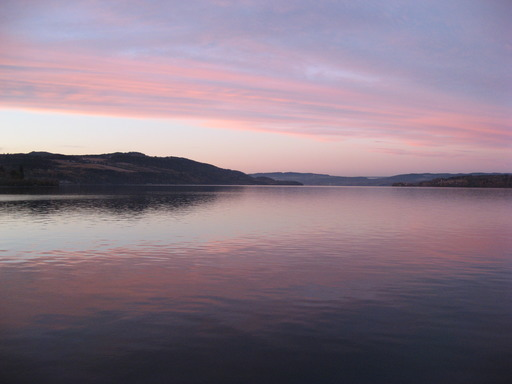
\includegraphics[keepaspectratio,height=7.75em]{NorNet-Configuration-Images/Hoegskolen_i_Gjoevik.jpeg}}} & \multicolumn{1}{|l|}{City} & \multicolumn{3}{|l|}{\index{Gjøvik}Gjøvik} \\* \cline{5-5}\cline{6-6}\cline{7-7}\cline{8-8}
 \multicolumn{4}{|c|}{} & \multicolumn{1}{|l|}{Province} & \multicolumn{3}{|l|}{\index{Oppland}\includegraphics[keepaspectratio,height=0.8em]{NorNet-Configuration-Images/NO-Oppland.pdf}Oppland} \\* \cline{5-5}\cline{6-6}\cline{7-7}\cline{8-8}
 \multicolumn{4}{|c|}{} & \multicolumn{1}{|l|}{Country} & \multicolumn{3}{|l|}{\index{NO}\index{Norge}\includegraphics[keepaspectratio,height=0.8em]{NorNet-Configuration-Images/Flag-NO.pdf}Norge (NO)} \\* \cline{5-5}\cline{6-6}\cline{7-7}\cline{8-8}
 \multicolumn{4}{|c|}{} & \multicolumn{1}{|l|}{GPS/ГЛОНАСС} & \multicolumn{3}{|l|}{60.7896°N / 10.6817°E / 200.0m} \\* \cline{5-5}\cline{6-6}\cline{7-7}\cline{8-8}
 \multicolumn{4}{|c|}{} & \multicolumn{1}{|l|}{Short Name} & \multicolumn{3}{|l|}{\nomenclature{HiG}{Høgskolen i Gjøvik}\index{HiG|see{Høgskolen i Gjøvik}}HiG} \\* \cline{5-5}\cline{6-6}\cline{7-7}\cline{8-8}
 \multicolumn{4}{|c|}{} & \multicolumn{1}{|l|}{Domain} & \multicolumn{3}{|l|}{\index{hig.nornet}hig.nornet} \\* \cline{5-5}\cline{6-6}\cline{7-7}\cline{8-8}
 \multicolumn{4}{|c|}{} & \multicolumn{1}{|l|}{URL} & \multicolumn{3}{|l|}{\url{https://www.hig.no}} \\ \hline
 \multicolumn{2}{|p{8em}|}{Node} & \multicolumn{2}{|p{8em}|}{Sliver} & \multicolumn{2}{|p{8em}|}{Provider} & IPv4 & IPv6 \\ \hline
\endfirsthead
\hline
 \multicolumn{8}{|c|}{\textbf{Høgskolen i Gjøvik (continued)}} \\ \hline
 \multicolumn{2}{|p{8em}|}{Node} & \multicolumn{2}{|p{8em}|}{Sliver} & \multicolumn{2}{|p{8em}|}{Provider} & IPv4 & IPv6 \\ \hline
\endhead
 \multirow{8}{*}{\tiny{1}} & \multicolumn{3}{|c|}{\multirow{8}{*}{\tiny{tunnelbox}}} & \multicolumn{2}{|c|}{\multirow{4}{*}{\tiny{\href{https://www.uninett.no}{Uninett} (1)}}} & \tiny{128.39.49.154} & \tiny{2001:700:1d00:18::154} \\* \cline{7-7}\cline{8-8}
  & \multicolumn{3}{|c|}{} & \multicolumn{2}{|c|}{} & \tiny{10.1.3.1} & \tiny{2001:700:4100:103::1} \\* \cline{7-7}\cline{8-8}
  & \multicolumn{3}{|c|}{} & \multicolumn{2}{|c|}{} & Type: & fibre, business \\* \cline{7-7}\cline{8-8}
  & \multicolumn{3}{|c|}{} & \multicolumn{2}{|c|}{} & Down/Up:  & unspecified \\* \cline{5-5}\cline{6-6}\cline{7-7}\cline{8-8}
  & \multicolumn{3}{|c|}{} & \multicolumn{2}{|c|}{\multirow{4}{*}{\tiny{\href{http://www.powertech.no}{PowerTech} (9)}}} & \tiny{195.159.158.254} & \tiny{2001:840:490b::254} \\* \cline{7-7}\cline{8-8}
  & \multicolumn{3}{|c|}{} & \multicolumn{2}{|c|}{} & \tiny{10.9.3.1} & \tiny{2001:700:4100:903::1} \\* \cline{7-7}\cline{8-8}
  & \multicolumn{3}{|c|}{} & \multicolumn{2}{|c|}{} & Type: & ADSL, consumer \\* \cline{7-7}\cline{8-8}
  & \multicolumn{3}{|c|}{} & \multicolumn{2}{|c|}{} & Down/Up:  & unspecified \\ \hline
 \multirow{32}{*}{\tiny{100}} & \multicolumn{1}{|l|}{\multirow{32}{*}{\tiny{kapp}}} & \multicolumn{2}{|c|}{\multirow{2}{*}{\tiny{Root Context}}} & \multicolumn{2}{|c|}{\tiny{\href{https://www.uninett.no}{Uninett} (1)}} & \tiny{10.1.3.100} & \tiny{2001:700:4100:103::64} \\* \cline{5-5}\cline{6-6}\cline{7-7}\cline{8-8}
  &  & \multicolumn{2}{|c|}{} & \multicolumn{2}{|c|}{\tiny{\href{http://www.powertech.no}{PowerTech} (9)}} & \tiny{10.9.3.100} & \tiny{2001:700:4100:903::64} \\* \cline{3-3}\cline{4-4}\cline{5-5}\cline{6-6}\cline{7-7}\cline{8-8}
  &  & \multirow{2}{*}{\tiny{120}} & \multicolumn{1}{|l|}{\multirow{2}{*}{\tiny{srl-test}}} & \multicolumn{2}{|c|}{\tiny{\href{https://www.uninett.no}{Uninett} (1)}} & \tiny{10.1.3.120} & \tiny{2001:700:4100:103::78:64} \\* \cline{5-5}\cline{6-6}\cline{7-7}\cline{8-8}
  &  &  &  & \multicolumn{2}{|c|}{\tiny{\href{http://www.powertech.no}{PowerTech} (9)}} & \tiny{10.9.3.120} & \tiny{2001:700:4100:903::78:64} \\* \cline{3-3}\cline{4-4}\cline{5-5}\cline{6-6}\cline{7-7}\cline{8-8}
  &  & \multirow{2}{*}{\tiny{128}} & \multicolumn{1}{|l|}{\multirow{2}{*}{\tiny{hu-multipath}}} & \multicolumn{2}{|c|}{\tiny{\href{https://www.uninett.no}{Uninett} (1)}} & \tiny{10.1.3.128} & \tiny{2001:700:4100:103::80:64} \\* \cline{5-5}\cline{6-6}\cline{7-7}\cline{8-8}
  &  &  &  & \multicolumn{2}{|c|}{\tiny{\href{http://www.powertech.no}{PowerTech} (9)}} & \tiny{10.9.3.128} & \tiny{2001:700:4100:903::80:64} \\* \cline{3-3}\cline{4-4}\cline{5-5}\cline{6-6}\cline{7-7}\cline{8-8}
  &  & \multirow{2}{*}{\tiny{135}} & \multicolumn{1}{|l|}{\multirow{2}{*}{\tiny{tuda-sereon}}} & \multicolumn{2}{|c|}{\tiny{\href{https://www.uninett.no}{Uninett} (1)}} & \tiny{10.1.3.135} & \tiny{2001:700:4100:103::87:64} \\* \cline{5-5}\cline{6-6}\cline{7-7}\cline{8-8}
  &  &  &  & \multicolumn{2}{|c|}{\tiny{\href{http://www.powertech.no}{PowerTech} (9)}} & \tiny{10.9.3.135} & \tiny{2001:700:4100:903::87:64} \\* \cline{3-3}\cline{4-4}\cline{5-5}\cline{6-6}\cline{7-7}\cline{8-8}
  &  & \multirow{2}{*}{\tiny{138}} & \multicolumn{1}{|l|}{\multirow{2}{*}{\tiny{ntnu-test}}} & \multicolumn{2}{|c|}{\tiny{\href{https://www.uninett.no}{Uninett} (1)}} & \tiny{10.1.3.138} & \tiny{2001:700:4100:103::8a:64} \\* \cline{5-5}\cline{6-6}\cline{7-7}\cline{8-8}
  &  &  &  & \multicolumn{2}{|c|}{\tiny{\href{http://www.powertech.no}{PowerTech} (9)}} & \tiny{10.9.3.138} & \tiny{2001:700:4100:903::8a:64} \\* \cline{3-3}\cline{4-4}\cline{5-5}\cline{6-6}\cline{7-7}\cline{8-8}
  &  & \multirow{2}{*}{\tiny{145}} & \multicolumn{1}{|l|}{\multirow{2}{*}{\tiny{ude-multipath}}} & \multicolumn{2}{|c|}{\tiny{\href{https://www.uninett.no}{Uninett} (1)}} & \tiny{10.1.3.145} & \tiny{2001:700:4100:103::91:64} \\* \cline{5-5}\cline{6-6}\cline{7-7}\cline{8-8}
  &  &  &  & \multicolumn{2}{|c|}{\tiny{\href{http://www.powertech.no}{PowerTech} (9)}} & \tiny{10.9.3.145} & \tiny{2001:700:4100:903::91:64} \\* \cline{3-3}\cline{4-4}\cline{5-5}\cline{6-6}\cline{7-7}\cline{8-8}
  &  & \multirow{2}{*}{\tiny{147}} & \multicolumn{1}{|l|}{\multirow{2}{*}{\tiny{uib-mptcp}}} & \multicolumn{2}{|c|}{\tiny{\href{https://www.uninett.no}{Uninett} (1)}} & \tiny{10.1.3.147} & \tiny{2001:700:4100:103::93:64} \\* \cline{5-5}\cline{6-6}\cline{7-7}\cline{8-8}
  &  &  &  & \multicolumn{2}{|c|}{\tiny{\href{http://www.powertech.no}{PowerTech} (9)}} & \tiny{10.9.3.147} & \tiny{2001:700:4100:903::93:64} \\* \cline{3-3}\cline{4-4}\cline{5-5}\cline{6-6}\cline{7-7}\cline{8-8}
  &  & \multirow{2}{*}{\tiny{150}} & \multicolumn{1}{|l|}{\multirow{2}{*}{\tiny{srl-mptcp}}} & \multicolumn{2}{|c|}{\tiny{\href{https://www.uninett.no}{Uninett} (1)}} & \tiny{10.1.3.150} & \tiny{2001:700:4100:103::96:64} \\* \cline{5-5}\cline{6-6}\cline{7-7}\cline{8-8}
  &  &  &  & \multicolumn{2}{|c|}{\tiny{\href{http://www.powertech.no}{PowerTech} (9)}} & \tiny{10.9.3.150} & \tiny{2001:700:4100:903::96:64} \\* \cline{3-3}\cline{4-4}\cline{5-5}\cline{6-6}\cline{7-7}\cline{8-8}
  &  & \multirow{2}{*}{\tiny{151}} & \multicolumn{1}{|l|}{\multirow{2}{*}{\tiny{hu-xingzhou}}} & \multicolumn{2}{|c|}{\tiny{\href{https://www.uninett.no}{Uninett} (1)}} & \tiny{10.1.3.151} & \tiny{2001:700:4100:103::97:64} \\* \cline{5-5}\cline{6-6}\cline{7-7}\cline{8-8}
  &  &  &  & \multicolumn{2}{|c|}{\tiny{\href{http://www.powertech.no}{PowerTech} (9)}} & \tiny{10.9.3.151} & \tiny{2001:700:4100:903::97:64} \\* \cline{3-3}\cline{4-4}\cline{5-5}\cline{6-6}\cline{7-7}\cline{8-8}
  &  & \multirow{2}{*}{\tiny{154}} & \multicolumn{1}{|l|}{\multirow{2}{*}{\tiny{ude-delaytest}}} & \multicolumn{2}{|c|}{\tiny{\href{https://www.uninett.no}{Uninett} (1)}} & \tiny{10.1.3.154} & \tiny{2001:700:4100:103::9a:64} \\* \cline{5-5}\cline{6-6}\cline{7-7}\cline{8-8}
  &  &  &  & \multicolumn{2}{|c|}{\tiny{\href{http://www.powertech.no}{PowerTech} (9)}} & \tiny{10.9.3.154} & \tiny{2001:700:4100:903::9a:64} \\* \cline{3-3}\cline{4-4}\cline{5-5}\cline{6-6}\cline{7-7}\cline{8-8}
  &  & \multirow{2}{*}{\tiny{157}} & \multicolumn{1}{|l|}{\multirow{2}{*}{\tiny{srl-seattle}}} & \multicolumn{2}{|c|}{\tiny{\href{https://www.uninett.no}{Uninett} (1)}} & \tiny{10.1.3.157} & \tiny{2001:700:4100:103::9d:64} \\* \cline{5-5}\cline{6-6}\cline{7-7}\cline{8-8}
  &  &  &  & \multicolumn{2}{|c|}{\tiny{\href{http://www.powertech.no}{PowerTech} (9)}} & \tiny{10.9.3.157} & \tiny{2001:700:4100:903::9d:64} \\* \cline{3-3}\cline{4-4}\cline{5-5}\cline{6-6}\cline{7-7}\cline{8-8}
  &  & \multirow{2}{*}{\tiny{161}} & \multicolumn{1}{|l|}{\multirow{2}{*}{\tiny{kau-mptcpsecurity}}} & \multicolumn{2}{|c|}{\tiny{\href{https://www.uninett.no}{Uninett} (1)}} & \tiny{10.1.3.161} & \tiny{2001:700:4100:103::a1:64} \\* \cline{5-5}\cline{6-6}\cline{7-7}\cline{8-8}
  &  &  &  & \multicolumn{2}{|c|}{\tiny{\href{http://www.powertech.no}{PowerTech} (9)}} & \tiny{10.9.3.161} & \tiny{2001:700:4100:903::a1:64} \\* \cline{3-3}\cline{4-4}\cline{5-5}\cline{6-6}\cline{7-7}\cline{8-8}
  &  & \multirow{2}{*}{\tiny{171}} & \multicolumn{1}{|l|}{\multirow{2}{*}{\tiny{haw-cmt}}} & \multicolumn{2}{|c|}{\tiny{\href{https://www.uninett.no}{Uninett} (1)}} & \tiny{10.1.3.171} & \tiny{2001:700:4100:103::ab:64} \\* \cline{5-5}\cline{6-6}\cline{7-7}\cline{8-8}
  &  &  &  & \multicolumn{2}{|c|}{\tiny{\href{http://www.powertech.no}{PowerTech} (9)}} & \tiny{10.9.3.171} & \tiny{2001:700:4100:903::ab:64} \\* \cline{3-3}\cline{4-4}\cline{5-5}\cline{6-6}\cline{7-7}\cline{8-8}
  &  & \multirow{2}{*}{\tiny{175}} & \multicolumn{1}{|l|}{\multirow{2}{*}{\tiny{srl-thuen}}} & \multicolumn{2}{|c|}{\tiny{\href{https://www.uninett.no}{Uninett} (1)}} & \tiny{10.1.3.175} & \tiny{2001:700:4100:103::af:64} \\* \cline{5-5}\cline{6-6}\cline{7-7}\cline{8-8}
  &  &  &  & \multicolumn{2}{|c|}{\tiny{\href{http://www.powertech.no}{PowerTech} (9)}} & \tiny{10.9.3.175} & \tiny{2001:700:4100:903::af:64} \\* \cline{3-3}\cline{4-4}\cline{5-5}\cline{6-6}\cline{7-7}\cline{8-8}
  &  & \multirow{2}{*}{\tiny{179}} & \multicolumn{1}{|l|}{\multirow{2}{*}{\tiny{hu-zhoufeng}}} & \multicolumn{2}{|c|}{\tiny{\href{https://www.uninett.no}{Uninett} (1)}} & \tiny{10.1.3.179} & \tiny{2001:700:4100:103::b3:64} \\* \cline{5-5}\cline{6-6}\cline{7-7}\cline{8-8}
  &  &  &  & \multicolumn{2}{|c|}{\tiny{\href{http://www.powertech.no}{PowerTech} (9)}} & \tiny{10.9.3.179} & \tiny{2001:700:4100:903::b3:64} \\* \cline{3-3}\cline{4-4}\cline{5-5}\cline{6-6}\cline{7-7}\cline{8-8}
  &  & \multirow{2}{*}{\tiny{191}} & \multicolumn{1}{|l|}{\multirow{2}{*}{\tiny{srl-nndemo}}} & \multicolumn{2}{|c|}{\tiny{\href{https://www.uninett.no}{Uninett} (1)}} & \tiny{10.1.3.191} & \tiny{2001:700:4100:103::bf:64} \\* \cline{5-5}\cline{6-6}\cline{7-7}\cline{8-8}
  &  &  &  & \multicolumn{2}{|c|}{\tiny{\href{http://www.powertech.no}{PowerTech} (9)}} & \tiny{10.9.3.191} & \tiny{2001:700:4100:903::bf:64} \\ \hline
 \multirow{26}{*}{\tiny{101}} & \multicolumn{1}{|l|}{\multirow{26}{*}{\tiny{eina}}} & \multicolumn{2}{|c|}{\multirow{2}{*}{\tiny{Root Context}}} & \multicolumn{2}{|c|}{\tiny{\href{https://www.uninett.no}{Uninett} (1)}} & \tiny{10.1.3.101} & \tiny{2001:700:4100:103::65} \\* \cline{5-5}\cline{6-6}\cline{7-7}\cline{8-8}
  &  & \multicolumn{2}{|c|}{} & \multicolumn{2}{|c|}{\tiny{\href{http://www.powertech.no}{PowerTech} (9)}} & \tiny{10.9.3.101} & \tiny{2001:700:4100:903::65} \\* \cline{3-3}\cline{4-4}\cline{5-5}\cline{6-6}\cline{7-7}\cline{8-8}
  &  & \multirow{2}{*}{\tiny{117}} & \multicolumn{1}{|l|}{\multirow{2}{*}{\tiny{hu-jerry}}} & \multicolumn{2}{|c|}{\tiny{\href{https://www.uninett.no}{Uninett} (1)}} & \tiny{10.1.3.117} & \tiny{2001:700:4100:103::75:65} \\* \cline{5-5}\cline{6-6}\cline{7-7}\cline{8-8}
  &  &  &  & \multicolumn{2}{|c|}{\tiny{\href{http://www.powertech.no}{PowerTech} (9)}} & \tiny{10.9.3.117} & \tiny{2001:700:4100:903::75:65} \\* \cline{3-3}\cline{4-4}\cline{5-5}\cline{6-6}\cline{7-7}\cline{8-8}
  &  & \multirow{2}{*}{\tiny{125}} & \multicolumn{1}{|l|}{\multirow{2}{*}{\tiny{srl-test}}} & \multicolumn{2}{|c|}{\tiny{\href{https://www.uninett.no}{Uninett} (1)}} & \tiny{10.1.3.125} & \tiny{2001:700:4100:103::7d:65} \\* \cline{5-5}\cline{6-6}\cline{7-7}\cline{8-8}
  &  &  &  & \multicolumn{2}{|c|}{\tiny{\href{http://www.powertech.no}{PowerTech} (9)}} & \tiny{10.9.3.125} & \tiny{2001:700:4100:903::7d:65} \\* \cline{3-3}\cline{4-4}\cline{5-5}\cline{6-6}\cline{7-7}\cline{8-8}
  &  & \multirow{2}{*}{\tiny{127}} & \multicolumn{1}{|l|}{\multirow{2}{*}{\tiny{hu-multipath}}} & \multicolumn{2}{|c|}{\tiny{\href{https://www.uninett.no}{Uninett} (1)}} & \tiny{10.1.3.127} & \tiny{2001:700:4100:103::7f:65} \\* \cline{5-5}\cline{6-6}\cline{7-7}\cline{8-8}
  &  &  &  & \multicolumn{2}{|c|}{\tiny{\href{http://www.powertech.no}{PowerTech} (9)}} & \tiny{10.9.3.127} & \tiny{2001:700:4100:903::7f:65} \\* \cline{3-3}\cline{4-4}\cline{5-5}\cline{6-6}\cline{7-7}\cline{8-8}
  &  & \multirow{2}{*}{\tiny{131}} & \multicolumn{1}{|l|}{\multirow{2}{*}{\tiny{kau-multipath}}} & \multicolumn{2}{|c|}{\tiny{\href{https://www.uninett.no}{Uninett} (1)}} & \tiny{10.1.3.131} & \tiny{2001:700:4100:103::83:65} \\* \cline{5-5}\cline{6-6}\cline{7-7}\cline{8-8}
  &  &  &  & \multicolumn{2}{|c|}{\tiny{\href{http://www.powertech.no}{PowerTech} (9)}} & \tiny{10.9.3.131} & \tiny{2001:700:4100:903::83:65} \\* \cline{3-3}\cline{4-4}\cline{5-5}\cline{6-6}\cline{7-7}\cline{8-8}
  &  & \multirow{2}{*}{\tiny{143}} & \multicolumn{1}{|l|}{\multirow{2}{*}{\tiny{ntnu-test}}} & \multicolumn{2}{|c|}{\tiny{\href{https://www.uninett.no}{Uninett} (1)}} & \tiny{10.1.3.143} & \tiny{2001:700:4100:103::8f:65} \\* \cline{5-5}\cline{6-6}\cline{7-7}\cline{8-8}
  &  &  &  & \multicolumn{2}{|c|}{\tiny{\href{http://www.powertech.no}{PowerTech} (9)}} & \tiny{10.9.3.143} & \tiny{2001:700:4100:903::8f:65} \\* \cline{3-3}\cline{4-4}\cline{5-5}\cline{6-6}\cline{7-7}\cline{8-8}
  &  & \multirow{2}{*}{\tiny{155}} & \multicolumn{1}{|l|}{\multirow{2}{*}{\tiny{srl-queuing}}} & \multicolumn{2}{|c|}{\tiny{\href{https://www.uninett.no}{Uninett} (1)}} & \tiny{10.1.3.155} & \tiny{2001:700:4100:103::9b:65} \\* \cline{5-5}\cline{6-6}\cline{7-7}\cline{8-8}
  &  &  &  & \multicolumn{2}{|c|}{\tiny{\href{http://www.powertech.no}{PowerTech} (9)}} & \tiny{10.9.3.155} & \tiny{2001:700:4100:903::9b:65} \\* \cline{3-3}\cline{4-4}\cline{5-5}\cline{6-6}\cline{7-7}\cline{8-8}
  &  & \multirow{2}{*}{\tiny{162}} & \multicolumn{1}{|l|}{\multirow{2}{*}{\tiny{hu-yuyintan}}} & \multicolumn{2}{|c|}{\tiny{\href{https://www.uninett.no}{Uninett} (1)}} & \tiny{10.1.3.162} & \tiny{2001:700:4100:103::a2:65} \\* \cline{5-5}\cline{6-6}\cline{7-7}\cline{8-8}
  &  &  &  & \multicolumn{2}{|c|}{\tiny{\href{http://www.powertech.no}{PowerTech} (9)}} & \tiny{10.9.3.162} & \tiny{2001:700:4100:903::a2:65} \\* \cline{3-3}\cline{4-4}\cline{5-5}\cline{6-6}\cline{7-7}\cline{8-8}
  &  & \multirow{2}{*}{\tiny{165}} & \multicolumn{1}{|l|}{\multirow{2}{*}{\tiny{hu-zhoufeng}}} & \multicolumn{2}{|c|}{\tiny{\href{https://www.uninett.no}{Uninett} (1)}} & \tiny{10.1.3.165} & \tiny{2001:700:4100:103::a5:65} \\* \cline{5-5}\cline{6-6}\cline{7-7}\cline{8-8}
  &  &  &  & \multicolumn{2}{|c|}{\tiny{\href{http://www.powertech.no}{PowerTech} (9)}} & \tiny{10.9.3.165} & \tiny{2001:700:4100:903::a5:65} \\* \cline{3-3}\cline{4-4}\cline{5-5}\cline{6-6}\cline{7-7}\cline{8-8}
  &  & \multirow{2}{*}{\tiny{166}} & \multicolumn{1}{|l|}{\multirow{2}{*}{\tiny{hu-xingzhou}}} & \multicolumn{2}{|c|}{\tiny{\href{https://www.uninett.no}{Uninett} (1)}} & \tiny{10.1.3.166} & \tiny{2001:700:4100:103::a6:65} \\* \cline{5-5}\cline{6-6}\cline{7-7}\cline{8-8}
  &  &  &  & \multicolumn{2}{|c|}{\tiny{\href{http://www.powertech.no}{PowerTech} (9)}} & \tiny{10.9.3.166} & \tiny{2001:700:4100:903::a6:65} \\* \cline{3-3}\cline{4-4}\cline{5-5}\cline{6-6}\cline{7-7}\cline{8-8}
  &  & \multirow{2}{*}{\tiny{180}} & \multicolumn{1}{|l|}{\multirow{2}{*}{\tiny{tuda-sereon}}} & \multicolumn{2}{|c|}{\tiny{\href{https://www.uninett.no}{Uninett} (1)}} & \tiny{10.1.3.180} & \tiny{2001:700:4100:103::b4:65} \\* \cline{5-5}\cline{6-6}\cline{7-7}\cline{8-8}
  &  &  &  & \multicolumn{2}{|c|}{\tiny{\href{http://www.powertech.no}{PowerTech} (9)}} & \tiny{10.9.3.180} & \tiny{2001:700:4100:903::b4:65} \\* \cline{3-3}\cline{4-4}\cline{5-5}\cline{6-6}\cline{7-7}\cline{8-8}
  &  & \multirow{2}{*}{\tiny{184}} & \multicolumn{1}{|l|}{\multirow{2}{*}{\tiny{hu-hanbaokuang}}} & \multicolumn{2}{|c|}{\tiny{\href{https://www.uninett.no}{Uninett} (1)}} & \tiny{10.1.3.184} & \tiny{2001:700:4100:103::b8:65} \\* \cline{5-5}\cline{6-6}\cline{7-7}\cline{8-8}
  &  &  &  & \multicolumn{2}{|c|}{\tiny{\href{http://www.powertech.no}{PowerTech} (9)}} & \tiny{10.9.3.184} & \tiny{2001:700:4100:903::b8:65} \\* \cline{3-3}\cline{4-4}\cline{5-5}\cline{6-6}\cline{7-7}\cline{8-8}
  &  & \multirow{2}{*}{\tiny{194}} & \multicolumn{1}{|l|}{\multirow{2}{*}{\tiny{hu-tanqilin}}} & \multicolumn{2}{|c|}{\tiny{\href{https://www.uninett.no}{Uninett} (1)}} & \tiny{10.1.3.194} & \tiny{2001:700:4100:103::c2:65} \\* \cline{5-5}\cline{6-6}\cline{7-7}\cline{8-8}
  &  &  &  & \multicolumn{2}{|c|}{\tiny{\href{http://www.powertech.no}{PowerTech} (9)}} & \tiny{10.9.3.194} & \tiny{2001:700:4100:903::c2:65} \\ \hline
 \multirow{20}{*}{\tiny{102}} & \multicolumn{1}{|l|}{\multirow{20}{*}{\tiny{raufoss}}} & \multicolumn{2}{|c|}{\multirow{2}{*}{\tiny{Root Context}}} & \multicolumn{2}{|c|}{\tiny{\href{https://www.uninett.no}{Uninett} (1)}} & \tiny{10.1.3.102} & \tiny{2001:700:4100:103::66} \\* \cline{5-5}\cline{6-6}\cline{7-7}\cline{8-8}
  &  & \multicolumn{2}{|c|}{} & \multicolumn{2}{|c|}{\tiny{\href{http://www.powertech.no}{PowerTech} (9)}} & \tiny{10.9.3.102} & \tiny{2001:700:4100:903::66} \\* \cline{3-3}\cline{4-4}\cline{5-5}\cline{6-6}\cline{7-7}\cline{8-8}
  &  & \multirow{2}{*}{\tiny{119}} & \multicolumn{1}{|l|}{\multirow{2}{*}{\tiny{tuda-sereon}}} & \multicolumn{2}{|c|}{\tiny{\href{https://www.uninett.no}{Uninett} (1)}} & \tiny{10.1.3.119} & \tiny{2001:700:4100:103::77:66} \\* \cline{5-5}\cline{6-6}\cline{7-7}\cline{8-8}
  &  &  &  & \multicolumn{2}{|c|}{\tiny{\href{http://www.powertech.no}{PowerTech} (9)}} & \tiny{10.9.3.119} & \tiny{2001:700:4100:903::77:66} \\* \cline{3-3}\cline{4-4}\cline{5-5}\cline{6-6}\cline{7-7}\cline{8-8}
  &  & \multirow{2}{*}{\tiny{123}} & \multicolumn{1}{|l|}{\multirow{2}{*}{\tiny{srl-test}}} & \multicolumn{2}{|c|}{\tiny{\href{https://www.uninett.no}{Uninett} (1)}} & \tiny{10.1.3.123} & \tiny{2001:700:4100:103::7b:66} \\* \cline{5-5}\cline{6-6}\cline{7-7}\cline{8-8}
  &  &  &  & \multicolumn{2}{|c|}{\tiny{\href{http://www.powertech.no}{PowerTech} (9)}} & \tiny{10.9.3.123} & \tiny{2001:700:4100:903::7b:66} \\* \cline{3-3}\cline{4-4}\cline{5-5}\cline{6-6}\cline{7-7}\cline{8-8}
  &  & \multirow{2}{*}{\tiny{129}} & \multicolumn{1}{|l|}{\multirow{2}{*}{\tiny{kau-multipath}}} & \multicolumn{2}{|c|}{\tiny{\href{https://www.uninett.no}{Uninett} (1)}} & \tiny{10.1.3.129} & \tiny{2001:700:4100:103::81:66} \\* \cline{5-5}\cline{6-6}\cline{7-7}\cline{8-8}
  &  &  &  & \multicolumn{2}{|c|}{\tiny{\href{http://www.powertech.no}{PowerTech} (9)}} & \tiny{10.9.3.129} & \tiny{2001:700:4100:903::81:66} \\* \cline{3-3}\cline{4-4}\cline{5-5}\cline{6-6}\cline{7-7}\cline{8-8}
  &  & \multirow{2}{*}{\tiny{137}} & \multicolumn{1}{|l|}{\multirow{2}{*}{\tiny{hu-multipath}}} & \multicolumn{2}{|c|}{\tiny{\href{https://www.uninett.no}{Uninett} (1)}} & \tiny{10.1.3.137} & \tiny{2001:700:4100:103::89:66} \\* \cline{5-5}\cline{6-6}\cline{7-7}\cline{8-8}
  &  &  &  & \multicolumn{2}{|c|}{\tiny{\href{http://www.powertech.no}{PowerTech} (9)}} & \tiny{10.9.3.137} & \tiny{2001:700:4100:903::89:66} \\* \cline{3-3}\cline{4-4}\cline{5-5}\cline{6-6}\cline{7-7}\cline{8-8}
  &  & \multirow{2}{*}{\tiny{141}} & \multicolumn{1}{|l|}{\multirow{2}{*}{\tiny{ntnu-test}}} & \multicolumn{2}{|c|}{\tiny{\href{https://www.uninett.no}{Uninett} (1)}} & \tiny{10.1.3.141} & \tiny{2001:700:4100:103::8d:66} \\* \cline{5-5}\cline{6-6}\cline{7-7}\cline{8-8}
  &  &  &  & \multicolumn{2}{|c|}{\tiny{\href{http://www.powertech.no}{PowerTech} (9)}} & \tiny{10.9.3.141} & \tiny{2001:700:4100:903::8d:66} \\* \cline{3-3}\cline{4-4}\cline{5-5}\cline{6-6}\cline{7-7}\cline{8-8}
  &  & \multirow{2}{*}{\tiny{156}} & \multicolumn{1}{|l|}{\multirow{2}{*}{\tiny{srl-nndemo}}} & \multicolumn{2}{|c|}{\tiny{\href{https://www.uninett.no}{Uninett} (1)}} & \tiny{10.1.3.156} & \tiny{2001:700:4100:103::9c:66} \\* \cline{5-5}\cline{6-6}\cline{7-7}\cline{8-8}
  &  &  &  & \multicolumn{2}{|c|}{\tiny{\href{http://www.powertech.no}{PowerTech} (9)}} & \tiny{10.9.3.156} & \tiny{2001:700:4100:903::9c:66} \\* \cline{3-3}\cline{4-4}\cline{5-5}\cline{6-6}\cline{7-7}\cline{8-8}
  &  & \multirow{2}{*}{\tiny{167}} & \multicolumn{1}{|l|}{\multirow{2}{*}{\tiny{srl-mptcp}}} & \multicolumn{2}{|c|}{\tiny{\href{https://www.uninett.no}{Uninett} (1)}} & \tiny{10.1.3.167} & \tiny{2001:700:4100:103::a7:66} \\* \cline{5-5}\cline{6-6}\cline{7-7}\cline{8-8}
  &  &  &  & \multicolumn{2}{|c|}{\tiny{\href{http://www.powertech.no}{PowerTech} (9)}} & \tiny{10.9.3.167} & \tiny{2001:700:4100:903::a7:66} \\* \cline{3-3}\cline{4-4}\cline{5-5}\cline{6-6}\cline{7-7}\cline{8-8}
  &  & \multirow{2}{*}{\tiny{181}} & \multicolumn{1}{|l|}{\multirow{2}{*}{\tiny{srl-seattle}}} & \multicolumn{2}{|c|}{\tiny{\href{https://www.uninett.no}{Uninett} (1)}} & \tiny{10.1.3.181} & \tiny{2001:700:4100:103::b5:66} \\* \cline{5-5}\cline{6-6}\cline{7-7}\cline{8-8}
  &  &  &  & \multicolumn{2}{|c|}{\tiny{\href{http://www.powertech.no}{PowerTech} (9)}} & \tiny{10.9.3.181} & \tiny{2001:700:4100:903::b5:66} \\* \cline{3-3}\cline{4-4}\cline{5-5}\cline{6-6}\cline{7-7}\cline{8-8}
  &  & \multirow{2}{*}{\tiny{195}} & \multicolumn{1}{|l|}{\multirow{2}{*}{\tiny{hu-tanqilin}}} & \multicolumn{2}{|c|}{\tiny{\href{https://www.uninett.no}{Uninett} (1)}} & \tiny{10.1.3.195} & \tiny{2001:700:4100:103::c3:66} \\* \cline{5-5}\cline{6-6}\cline{7-7}\cline{8-8}
  &  &  &  & \multicolumn{2}{|c|}{\tiny{\href{http://www.powertech.no}{PowerTech} (9)}} & \tiny{10.9.3.195} & \tiny{2001:700:4100:903::c3:66} \\ \hline
 \multirow{30}{*}{\tiny{103}} & \multicolumn{1}{|l|}{\multirow{30}{*}{\tiny{reinsvoll}}} & \multicolumn{2}{|c|}{\multirow{2}{*}{\tiny{Root Context}}} & \multicolumn{2}{|c|}{\tiny{\href{https://www.uninett.no}{Uninett} (1)}} & \tiny{10.1.3.103} & \tiny{2001:700:4100:103::67} \\* \cline{5-5}\cline{6-6}\cline{7-7}\cline{8-8}
  &  & \multicolumn{2}{|c|}{} & \multicolumn{2}{|c|}{\tiny{\href{http://www.powertech.no}{PowerTech} (9)}} & \tiny{10.9.3.103} & \tiny{2001:700:4100:903::67} \\* \cline{3-3}\cline{4-4}\cline{5-5}\cline{6-6}\cline{7-7}\cline{8-8}
  &  & \multirow{2}{*}{\tiny{115}} & \multicolumn{1}{|l|}{\multirow{2}{*}{\tiny{srl-mptcp}}} & \multicolumn{2}{|c|}{\tiny{\href{https://www.uninett.no}{Uninett} (1)}} & \tiny{10.1.3.115} & \tiny{2001:700:4100:103::73:67} \\* \cline{5-5}\cline{6-6}\cline{7-7}\cline{8-8}
  &  &  &  & \multicolumn{2}{|c|}{\tiny{\href{http://www.powertech.no}{PowerTech} (9)}} & \tiny{10.9.3.115} & \tiny{2001:700:4100:903::73:67} \\* \cline{3-3}\cline{4-4}\cline{5-5}\cline{6-6}\cline{7-7}\cline{8-8}
  &  & \multirow{2}{*}{\tiny{121}} & \multicolumn{1}{|l|}{\multirow{2}{*}{\tiny{srl-test}}} & \multicolumn{2}{|c|}{\tiny{\href{https://www.uninett.no}{Uninett} (1)}} & \tiny{10.1.3.121} & \tiny{2001:700:4100:103::79:67} \\* \cline{5-5}\cline{6-6}\cline{7-7}\cline{8-8}
  &  &  &  & \multicolumn{2}{|c|}{\tiny{\href{http://www.powertech.no}{PowerTech} (9)}} & \tiny{10.9.3.121} & \tiny{2001:700:4100:903::79:67} \\* \cline{3-3}\cline{4-4}\cline{5-5}\cline{6-6}\cline{7-7}\cline{8-8}
  &  & \multirow{2}{*}{\tiny{126}} & \multicolumn{1}{|l|}{\multirow{2}{*}{\tiny{srl-netperformance}}} & \multicolumn{2}{|c|}{\tiny{\href{https://www.uninett.no}{Uninett} (1)}} & \tiny{10.1.3.126} & \tiny{2001:700:4100:103::7e:67} \\* \cline{5-5}\cline{6-6}\cline{7-7}\cline{8-8}
  &  &  &  & \multicolumn{2}{|c|}{\tiny{\href{http://www.powertech.no}{PowerTech} (9)}} & \tiny{10.9.3.126} & \tiny{2001:700:4100:903::7e:67} \\* \cline{3-3}\cline{4-4}\cline{5-5}\cline{6-6}\cline{7-7}\cline{8-8}
  &  & \multirow{2}{*}{\tiny{132}} & \multicolumn{1}{|l|}{\multirow{2}{*}{\tiny{srl-cps}}} & \multicolumn{2}{|c|}{\tiny{\href{https://www.uninett.no}{Uninett} (1)}} & \tiny{10.1.3.132} & \tiny{2001:700:4100:103::84:67} \\* \cline{5-5}\cline{6-6}\cline{7-7}\cline{8-8}
  &  &  &  & \multicolumn{2}{|c|}{\tiny{\href{http://www.powertech.no}{PowerTech} (9)}} & \tiny{10.9.3.132} & \tiny{2001:700:4100:903::84:67} \\* \cline{3-3}\cline{4-4}\cline{5-5}\cline{6-6}\cline{7-7}\cline{8-8}
  &  & \multirow{2}{*}{\tiny{139}} & \multicolumn{1}{|l|}{\multirow{2}{*}{\tiny{ntnu-test}}} & \multicolumn{2}{|c|}{\tiny{\href{https://www.uninett.no}{Uninett} (1)}} & \tiny{10.1.3.139} & \tiny{2001:700:4100:103::8b:67} \\* \cline{5-5}\cline{6-6}\cline{7-7}\cline{8-8}
  &  &  &  & \multicolumn{2}{|c|}{\tiny{\href{http://www.powertech.no}{PowerTech} (9)}} & \tiny{10.9.3.139} & \tiny{2001:700:4100:903::8b:67} \\* \cline{3-3}\cline{4-4}\cline{5-5}\cline{6-6}\cline{7-7}\cline{8-8}
  &  & \multirow{2}{*}{\tiny{146}} & \multicolumn{1}{|l|}{\multirow{2}{*}{\tiny{hu-jiangshuihong}}} & \multicolumn{2}{|c|}{\tiny{\href{https://www.uninett.no}{Uninett} (1)}} & \tiny{10.1.3.146} & \tiny{2001:700:4100:103::92:67} \\* \cline{5-5}\cline{6-6}\cline{7-7}\cline{8-8}
  &  &  &  & \multicolumn{2}{|c|}{\tiny{\href{http://www.powertech.no}{PowerTech} (9)}} & \tiny{10.9.3.146} & \tiny{2001:700:4100:903::92:67} \\* \cline{3-3}\cline{4-4}\cline{5-5}\cline{6-6}\cline{7-7}\cline{8-8}
  &  & \multirow{2}{*}{\tiny{148}} & \multicolumn{1}{|l|}{\multirow{2}{*}{\tiny{hu-multipath}}} & \multicolumn{2}{|c|}{\tiny{\href{https://www.uninett.no}{Uninett} (1)}} & \tiny{10.1.3.148} & \tiny{2001:700:4100:103::94:67} \\* \cline{5-5}\cline{6-6}\cline{7-7}\cline{8-8}
  &  &  &  & \multicolumn{2}{|c|}{\tiny{\href{http://www.powertech.no}{PowerTech} (9)}} & \tiny{10.9.3.148} & \tiny{2001:700:4100:903::94:67} \\* \cline{3-3}\cline{4-4}\cline{5-5}\cline{6-6}\cline{7-7}\cline{8-8}
  &  & \multirow{2}{*}{\tiny{152}} & \multicolumn{1}{|l|}{\multirow{2}{*}{\tiny{ude-delaytest}}} & \multicolumn{2}{|c|}{\tiny{\href{https://www.uninett.no}{Uninett} (1)}} & \tiny{10.1.3.152} & \tiny{2001:700:4100:103::98:67} \\* \cline{5-5}\cline{6-6}\cline{7-7}\cline{8-8}
  &  &  &  & \multicolumn{2}{|c|}{\tiny{\href{http://www.powertech.no}{PowerTech} (9)}} & \tiny{10.9.3.152} & \tiny{2001:700:4100:903::98:67} \\* \cline{3-3}\cline{4-4}\cline{5-5}\cline{6-6}\cline{7-7}\cline{8-8}
  &  & \multirow{2}{*}{\tiny{159}} & \multicolumn{1}{|l|}{\multirow{2}{*}{\tiny{tuda-sereon}}} & \multicolumn{2}{|c|}{\tiny{\href{https://www.uninett.no}{Uninett} (1)}} & \tiny{10.1.3.159} & \tiny{2001:700:4100:103::9f:67} \\* \cline{5-5}\cline{6-6}\cline{7-7}\cline{8-8}
  &  &  &  & \multicolumn{2}{|c|}{\tiny{\href{http://www.powertech.no}{PowerTech} (9)}} & \tiny{10.9.3.159} & \tiny{2001:700:4100:903::9f:67} \\* \cline{3-3}\cline{4-4}\cline{5-5}\cline{6-6}\cline{7-7}\cline{8-8}
  &  & \multirow{2}{*}{\tiny{174}} & \multicolumn{1}{|l|}{\multirow{2}{*}{\tiny{srl-thuen}}} & \multicolumn{2}{|c|}{\tiny{\href{https://www.uninett.no}{Uninett} (1)}} & \tiny{10.1.3.174} & \tiny{2001:700:4100:103::ae:67} \\* \cline{5-5}\cline{6-6}\cline{7-7}\cline{8-8}
  &  &  &  & \multicolumn{2}{|c|}{\tiny{\href{http://www.powertech.no}{PowerTech} (9)}} & \tiny{10.9.3.174} & \tiny{2001:700:4100:903::ae:67} \\* \cline{3-3}\cline{4-4}\cline{5-5}\cline{6-6}\cline{7-7}\cline{8-8}
  &  & \multirow{2}{*}{\tiny{176}} & \multicolumn{1}{|l|}{\multirow{2}{*}{\tiny{haw-cmt}}} & \multicolumn{2}{|c|}{\tiny{\href{https://www.uninett.no}{Uninett} (1)}} & \tiny{10.1.3.176} & \tiny{2001:700:4100:103::b0:67} \\* \cline{5-5}\cline{6-6}\cline{7-7}\cline{8-8}
  &  &  &  & \multicolumn{2}{|c|}{\tiny{\href{http://www.powertech.no}{PowerTech} (9)}} & \tiny{10.9.3.176} & \tiny{2001:700:4100:903::b0:67} \\* \cline{3-3}\cline{4-4}\cline{5-5}\cline{6-6}\cline{7-7}\cline{8-8}
  &  & \multirow{2}{*}{\tiny{178}} & \multicolumn{1}{|l|}{\multirow{2}{*}{\tiny{hu-zhoufeng}}} & \multicolumn{2}{|c|}{\tiny{\href{https://www.uninett.no}{Uninett} (1)}} & \tiny{10.1.3.178} & \tiny{2001:700:4100:103::b2:67} \\* \cline{5-5}\cline{6-6}\cline{7-7}\cline{8-8}
  &  &  &  & \multicolumn{2}{|c|}{\tiny{\href{http://www.powertech.no}{PowerTech} (9)}} & \tiny{10.9.3.178} & \tiny{2001:700:4100:903::b2:67} \\* \cline{3-3}\cline{4-4}\cline{5-5}\cline{6-6}\cline{7-7}\cline{8-8}
  &  & \multirow{2}{*}{\tiny{182}} & \multicolumn{1}{|l|}{\multirow{2}{*}{\tiny{hu-chengxi}}} & \multicolumn{2}{|c|}{\tiny{\href{https://www.uninett.no}{Uninett} (1)}} & \tiny{10.1.3.182} & \tiny{2001:700:4100:103::b6:67} \\* \cline{5-5}\cline{6-6}\cline{7-7}\cline{8-8}
  &  &  &  & \multicolumn{2}{|c|}{\tiny{\href{http://www.powertech.no}{PowerTech} (9)}} & \tiny{10.9.3.182} & \tiny{2001:700:4100:903::b6:67} \\* \cline{3-3}\cline{4-4}\cline{5-5}\cline{6-6}\cline{7-7}\cline{8-8}
  &  & \multirow{2}{*}{\tiny{198}} & \multicolumn{1}{|l|}{\multirow{2}{*}{\tiny{hu-kunwang}}} & \multicolumn{2}{|c|}{\tiny{\href{https://www.uninett.no}{Uninett} (1)}} & \tiny{10.1.3.198} & \tiny{2001:700:4100:103::c6:67} \\* \cline{5-5}\cline{6-6}\cline{7-7}\cline{8-8}
  &  &  &  & \multicolumn{2}{|c|}{\tiny{\href{http://www.powertech.no}{PowerTech} (9)}} & \tiny{10.9.3.198} & \tiny{2001:700:4100:903::c6:67} \\ \hline
 \multirow{38}{*}{\tiny{104}} & \multicolumn{1}{|l|}{\multirow{38}{*}{\tiny{skreia}}} & \multicolumn{2}{|c|}{\multirow{2}{*}{\tiny{Root Context}}} & \multicolumn{2}{|c|}{\tiny{\href{https://www.uninett.no}{Uninett} (1)}} & \tiny{10.1.3.104} & \tiny{2001:700:4100:103::68} \\* \cline{5-5}\cline{6-6}\cline{7-7}\cline{8-8}
  &  & \multicolumn{2}{|c|}{} & \multicolumn{2}{|c|}{\tiny{\href{http://www.powertech.no}{PowerTech} (9)}} & \tiny{10.9.3.104} & \tiny{2001:700:4100:903::68} \\* \cline{3-3}\cline{4-4}\cline{5-5}\cline{6-6}\cline{7-7}\cline{8-8}
  &  & \multirow{2}{*}{\tiny{116}} & \multicolumn{1}{|l|}{\multirow{2}{*}{\tiny{srl-mptcp}}} & \multicolumn{2}{|c|}{\tiny{\href{https://www.uninett.no}{Uninett} (1)}} & \tiny{10.1.3.116} & \tiny{2001:700:4100:103::74:68} \\* \cline{5-5}\cline{6-6}\cline{7-7}\cline{8-8}
  &  &  &  & \multicolumn{2}{|c|}{\tiny{\href{http://www.powertech.no}{PowerTech} (9)}} & \tiny{10.9.3.116} & \tiny{2001:700:4100:903::74:68} \\* \cline{3-3}\cline{4-4}\cline{5-5}\cline{6-6}\cline{7-7}\cline{8-8}
  &  & \multirow{2}{*}{\tiny{124}} & \multicolumn{1}{|l|}{\multirow{2}{*}{\tiny{srl-test}}} & \multicolumn{2}{|c|}{\tiny{\href{https://www.uninett.no}{Uninett} (1)}} & \tiny{10.1.3.124} & \tiny{2001:700:4100:103::7c:68} \\* \cline{5-5}\cline{6-6}\cline{7-7}\cline{8-8}
  &  &  &  & \multicolumn{2}{|c|}{\tiny{\href{http://www.powertech.no}{PowerTech} (9)}} & \tiny{10.9.3.124} & \tiny{2001:700:4100:903::7c:68} \\* \cline{3-3}\cline{4-4}\cline{5-5}\cline{6-6}\cline{7-7}\cline{8-8}
  &  & \multirow{2}{*}{\tiny{130}} & \multicolumn{1}{|l|}{\multirow{2}{*}{\tiny{srl-netperformance}}} & \multicolumn{2}{|c|}{\tiny{\href{https://www.uninett.no}{Uninett} (1)}} & \tiny{10.1.3.130} & \tiny{2001:700:4100:103::82:68} \\* \cline{5-5}\cline{6-6}\cline{7-7}\cline{8-8}
  &  &  &  & \multicolumn{2}{|c|}{\tiny{\href{http://www.powertech.no}{PowerTech} (9)}} & \tiny{10.9.3.130} & \tiny{2001:700:4100:903::82:68} \\* \cline{3-3}\cline{4-4}\cline{5-5}\cline{6-6}\cline{7-7}\cline{8-8}
  &  & \multirow{2}{*}{\tiny{134}} & \multicolumn{1}{|l|}{\multirow{2}{*}{\tiny{srl-cps}}} & \multicolumn{2}{|c|}{\tiny{\href{https://www.uninett.no}{Uninett} (1)}} & \tiny{10.1.3.134} & \tiny{2001:700:4100:103::86:68} \\* \cline{5-5}\cline{6-6}\cline{7-7}\cline{8-8}
  &  &  &  & \multicolumn{2}{|c|}{\tiny{\href{http://www.powertech.no}{PowerTech} (9)}} & \tiny{10.9.3.134} & \tiny{2001:700:4100:903::86:68} \\* \cline{3-3}\cline{4-4}\cline{5-5}\cline{6-6}\cline{7-7}\cline{8-8}
  &  & \multirow{2}{*}{\tiny{136}} & \multicolumn{1}{|l|}{\multirow{2}{*}{\tiny{ude-multipath}}} & \multicolumn{2}{|c|}{\tiny{\href{https://www.uninett.no}{Uninett} (1)}} & \tiny{10.1.3.136} & \tiny{2001:700:4100:103::88:68} \\* \cline{5-5}\cline{6-6}\cline{7-7}\cline{8-8}
  &  &  &  & \multicolumn{2}{|c|}{\tiny{\href{http://www.powertech.no}{PowerTech} (9)}} & \tiny{10.9.3.136} & \tiny{2001:700:4100:903::88:68} \\* \cline{3-3}\cline{4-4}\cline{5-5}\cline{6-6}\cline{7-7}\cline{8-8}
  &  & \multirow{2}{*}{\tiny{142}} & \multicolumn{1}{|l|}{\multirow{2}{*}{\tiny{ntnu-test}}} & \multicolumn{2}{|c|}{\tiny{\href{https://www.uninett.no}{Uninett} (1)}} & \tiny{10.1.3.142} & \tiny{2001:700:4100:103::8e:68} \\* \cline{5-5}\cline{6-6}\cline{7-7}\cline{8-8}
  &  &  &  & \multicolumn{2}{|c|}{\tiny{\href{http://www.powertech.no}{PowerTech} (9)}} & \tiny{10.9.3.142} & \tiny{2001:700:4100:903::8e:68} \\* \cline{3-3}\cline{4-4}\cline{5-5}\cline{6-6}\cline{7-7}\cline{8-8}
  &  & \multirow{2}{*}{\tiny{149}} & \multicolumn{1}{|l|}{\multirow{2}{*}{\tiny{hu-multipath}}} & \multicolumn{2}{|c|}{\tiny{\href{https://www.uninett.no}{Uninett} (1)}} & \tiny{10.1.3.149} & \tiny{2001:700:4100:103::95:68} \\* \cline{5-5}\cline{6-6}\cline{7-7}\cline{8-8}
  &  &  &  & \multicolumn{2}{|c|}{\tiny{\href{http://www.powertech.no}{PowerTech} (9)}} & \tiny{10.9.3.149} & \tiny{2001:700:4100:903::95:68} \\* \cline{3-3}\cline{4-4}\cline{5-5}\cline{6-6}\cline{7-7}\cline{8-8}
  &  & \multirow{2}{*}{\tiny{164}} & \multicolumn{1}{|l|}{\multirow{2}{*}{\tiny{tuda-sereon}}} & \multicolumn{2}{|c|}{\tiny{\href{https://www.uninett.no}{Uninett} (1)}} & \tiny{10.1.3.164} & \tiny{2001:700:4100:103::a4:68} \\* \cline{5-5}\cline{6-6}\cline{7-7}\cline{8-8}
  &  &  &  & \multicolumn{2}{|c|}{\tiny{\href{http://www.powertech.no}{PowerTech} (9)}} & \tiny{10.9.3.164} & \tiny{2001:700:4100:903::a4:68} \\* \cline{3-3}\cline{4-4}\cline{5-5}\cline{6-6}\cline{7-7}\cline{8-8}
  &  & \multirow{2}{*}{\tiny{168}} & \multicolumn{1}{|l|}{\multirow{2}{*}{\tiny{srl-queuing}}} & \multicolumn{2}{|c|}{\tiny{\href{https://www.uninett.no}{Uninett} (1)}} & \tiny{10.1.3.168} & \tiny{2001:700:4100:103::a8:68} \\* \cline{5-5}\cline{6-6}\cline{7-7}\cline{8-8}
  &  &  &  & \multicolumn{2}{|c|}{\tiny{\href{http://www.powertech.no}{PowerTech} (9)}} & \tiny{10.9.3.168} & \tiny{2001:700:4100:903::a8:68} \\* \cline{3-3}\cline{4-4}\cline{5-5}\cline{6-6}\cline{7-7}\cline{8-8}
  &  & \multirow{2}{*}{\tiny{169}} & \multicolumn{1}{|l|}{\multirow{2}{*}{\tiny{hu-zhoufeng}}} & \multicolumn{2}{|c|}{\tiny{\href{https://www.uninett.no}{Uninett} (1)}} & \tiny{10.1.3.169} & \tiny{2001:700:4100:103::a9:68} \\* \cline{5-5}\cline{6-6}\cline{7-7}\cline{8-8}
  &  &  &  & \multicolumn{2}{|c|}{\tiny{\href{http://www.powertech.no}{PowerTech} (9)}} & \tiny{10.9.3.169} & \tiny{2001:700:4100:903::a9:68} \\* \cline{3-3}\cline{4-4}\cline{5-5}\cline{6-6}\cline{7-7}\cline{8-8}
  &  & \multirow{2}{*}{\tiny{173}} & \multicolumn{1}{|l|}{\multirow{2}{*}{\tiny{srl-thuen}}} & \multicolumn{2}{|c|}{\tiny{\href{https://www.uninett.no}{Uninett} (1)}} & \tiny{10.1.3.173} & \tiny{2001:700:4100:103::ad:68} \\* \cline{5-5}\cline{6-6}\cline{7-7}\cline{8-8}
  &  &  &  & \multicolumn{2}{|c|}{\tiny{\href{http://www.powertech.no}{PowerTech} (9)}} & \tiny{10.9.3.173} & \tiny{2001:700:4100:903::ad:68} \\* \cline{3-3}\cline{4-4}\cline{5-5}\cline{6-6}\cline{7-7}\cline{8-8}
  &  & \multirow{2}{*}{\tiny{177}} & \multicolumn{1}{|l|}{\multirow{2}{*}{\tiny{haw-cmt}}} & \multicolumn{2}{|c|}{\tiny{\href{https://www.uninett.no}{Uninett} (1)}} & \tiny{10.1.3.177} & \tiny{2001:700:4100:103::b1:68} \\* \cline{5-5}\cline{6-6}\cline{7-7}\cline{8-8}
  &  &  &  & \multicolumn{2}{|c|}{\tiny{\href{http://www.powertech.no}{PowerTech} (9)}} & \tiny{10.9.3.177} & \tiny{2001:700:4100:903::b1:68} \\* \cline{3-3}\cline{4-4}\cline{5-5}\cline{6-6}\cline{7-7}\cline{8-8}
  &  & \multirow{2}{*}{\tiny{183}} & \multicolumn{1}{|l|}{\multirow{2}{*}{\tiny{hu-chengxi}}} & \multicolumn{2}{|c|}{\tiny{\href{https://www.uninett.no}{Uninett} (1)}} & \tiny{10.1.3.183} & \tiny{2001:700:4100:103::b7:68} \\* \cline{5-5}\cline{6-6}\cline{7-7}\cline{8-8}
  &  &  &  & \multicolumn{2}{|c|}{\tiny{\href{http://www.powertech.no}{PowerTech} (9)}} & \tiny{10.9.3.183} & \tiny{2001:700:4100:903::b7:68} \\* \cline{3-3}\cline{4-4}\cline{5-5}\cline{6-6}\cline{7-7}\cline{8-8}
  &  & \multirow{2}{*}{\tiny{185}} & \multicolumn{1}{|l|}{\multirow{2}{*}{\tiny{hu-hanbaokuang}}} & \multicolumn{2}{|c|}{\tiny{\href{https://www.uninett.no}{Uninett} (1)}} & \tiny{10.1.3.185} & \tiny{2001:700:4100:103::b9:68} \\* \cline{5-5}\cline{6-6}\cline{7-7}\cline{8-8}
  &  &  &  & \multicolumn{2}{|c|}{\tiny{\href{http://www.powertech.no}{PowerTech} (9)}} & \tiny{10.9.3.185} & \tiny{2001:700:4100:903::b9:68} \\* \cline{3-3}\cline{4-4}\cline{5-5}\cline{6-6}\cline{7-7}\cline{8-8}
  &  & \multirow{2}{*}{\tiny{186}} & \multicolumn{1}{|l|}{\multirow{2}{*}{\tiny{hu-yuyintan}}} & \multicolumn{2}{|c|}{\tiny{\href{https://www.uninett.no}{Uninett} (1)}} & \tiny{10.1.3.186} & \tiny{2001:700:4100:103::ba:68} \\* \cline{5-5}\cline{6-6}\cline{7-7}\cline{8-8}
  &  &  &  & \multicolumn{2}{|c|}{\tiny{\href{http://www.powertech.no}{PowerTech} (9)}} & \tiny{10.9.3.186} & \tiny{2001:700:4100:903::ba:68} \\* \cline{3-3}\cline{4-4}\cline{5-5}\cline{6-6}\cline{7-7}\cline{8-8}
  &  & \multirow{2}{*}{\tiny{189}} & \multicolumn{1}{|l|}{\multirow{2}{*}{\tiny{hu-jiangshuihong}}} & \multicolumn{2}{|c|}{\tiny{\href{https://www.uninett.no}{Uninett} (1)}} & \tiny{10.1.3.189} & \tiny{2001:700:4100:103::bd:68} \\* \cline{5-5}\cline{6-6}\cline{7-7}\cline{8-8}
  &  &  &  & \multicolumn{2}{|c|}{\tiny{\href{http://www.powertech.no}{PowerTech} (9)}} & \tiny{10.9.3.189} & \tiny{2001:700:4100:903::bd:68} \\* \cline{3-3}\cline{4-4}\cline{5-5}\cline{6-6}\cline{7-7}\cline{8-8}
  &  & \multirow{2}{*}{\tiny{190}} & \multicolumn{1}{|l|}{\multirow{2}{*}{\tiny{hu-fufa}}} & \multicolumn{2}{|c|}{\tiny{\href{https://www.uninett.no}{Uninett} (1)}} & \tiny{10.1.3.190} & \tiny{2001:700:4100:103::be:68} \\* \cline{5-5}\cline{6-6}\cline{7-7}\cline{8-8}
  &  &  &  & \multicolumn{2}{|c|}{\tiny{\href{http://www.powertech.no}{PowerTech} (9)}} & \tiny{10.9.3.190} & \tiny{2001:700:4100:903::be:68} \\* \cline{3-3}\cline{4-4}\cline{5-5}\cline{6-6}\cline{7-7}\cline{8-8}
  &  & \multirow{2}{*}{\tiny{197}} & \multicolumn{1}{|l|}{\multirow{2}{*}{\tiny{hu-kunwang}}} & \multicolumn{2}{|c|}{\tiny{\href{https://www.uninett.no}{Uninett} (1)}} & \tiny{10.1.3.197} & \tiny{2001:700:4100:103::c5:68} \\* \cline{5-5}\cline{6-6}\cline{7-7}\cline{8-8}
  &  &  &  & \multicolumn{2}{|c|}{\tiny{\href{http://www.powertech.no}{PowerTech} (9)}} & \tiny{10.9.3.197} & \tiny{2001:700:4100:903::c5:68} \\ \hline
 \multirow{20}{*}{\tiny{105}} & \multicolumn{1}{|l|}{\multirow{20}{*}{\tiny{lena}}} & \multicolumn{2}{|c|}{\multirow{2}{*}{\tiny{Root Context}}} & \multicolumn{2}{|c|}{\tiny{\href{https://www.uninett.no}{Uninett} (1)}} & \tiny{10.1.3.105} & \tiny{2001:700:4100:103::69} \\* \cline{5-5}\cline{6-6}\cline{7-7}\cline{8-8}
  &  & \multicolumn{2}{|c|}{} & \multicolumn{2}{|c|}{\tiny{\href{http://www.powertech.no}{PowerTech} (9)}} & \tiny{10.9.3.105} & \tiny{2001:700:4100:903::69} \\* \cline{3-3}\cline{4-4}\cline{5-5}\cline{6-6}\cline{7-7}\cline{8-8}
  &  & \multirow{2}{*}{\tiny{118}} & \multicolumn{1}{|l|}{\multirow{2}{*}{\tiny{tuda-sereon}}} & \multicolumn{2}{|c|}{\tiny{\href{https://www.uninett.no}{Uninett} (1)}} & \tiny{10.1.3.118} & \tiny{2001:700:4100:103::76:69} \\* \cline{5-5}\cline{6-6}\cline{7-7}\cline{8-8}
  &  &  &  & \multicolumn{2}{|c|}{\tiny{\href{http://www.powertech.no}{PowerTech} (9)}} & \tiny{10.9.3.118} & \tiny{2001:700:4100:903::76:69} \\* \cline{3-3}\cline{4-4}\cline{5-5}\cline{6-6}\cline{7-7}\cline{8-8}
  &  & \multirow{2}{*}{\tiny{122}} & \multicolumn{1}{|l|}{\multirow{2}{*}{\tiny{srl-test}}} & \multicolumn{2}{|c|}{\tiny{\href{https://www.uninett.no}{Uninett} (1)}} & \tiny{10.1.3.122} & \tiny{2001:700:4100:103::7a:69} \\* \cline{5-5}\cline{6-6}\cline{7-7}\cline{8-8}
  &  &  &  & \multicolumn{2}{|c|}{\tiny{\href{http://www.powertech.no}{PowerTech} (9)}} & \tiny{10.9.3.122} & \tiny{2001:700:4100:903::7a:69} \\* \cline{3-3}\cline{4-4}\cline{5-5}\cline{6-6}\cline{7-7}\cline{8-8}
  &  & \multirow{2}{*}{\tiny{133}} & \multicolumn{1}{|l|}{\multirow{2}{*}{\tiny{hu-multipath}}} & \multicolumn{2}{|c|}{\tiny{\href{https://www.uninett.no}{Uninett} (1)}} & \tiny{10.1.3.133} & \tiny{2001:700:4100:103::85:69} \\* \cline{5-5}\cline{6-6}\cline{7-7}\cline{8-8}
  &  &  &  & \multicolumn{2}{|c|}{\tiny{\href{http://www.powertech.no}{PowerTech} (9)}} & \tiny{10.9.3.133} & \tiny{2001:700:4100:903::85:69} \\* \cline{3-3}\cline{4-4}\cline{5-5}\cline{6-6}\cline{7-7}\cline{8-8}
  &  & \multirow{2}{*}{\tiny{140}} & \multicolumn{1}{|l|}{\multirow{2}{*}{\tiny{ntnu-test}}} & \multicolumn{2}{|c|}{\tiny{\href{https://www.uninett.no}{Uninett} (1)}} & \tiny{10.1.3.140} & \tiny{2001:700:4100:103::8c:69} \\* \cline{5-5}\cline{6-6}\cline{7-7}\cline{8-8}
  &  &  &  & \multicolumn{2}{|c|}{\tiny{\href{http://www.powertech.no}{PowerTech} (9)}} & \tiny{10.9.3.140} & \tiny{2001:700:4100:903::8c:69} \\* \cline{3-3}\cline{4-4}\cline{5-5}\cline{6-6}\cline{7-7}\cline{8-8}
  &  & \multirow{2}{*}{\tiny{144}} & \multicolumn{1}{|l|}{\multirow{2}{*}{\tiny{uib-mptcp}}} & \multicolumn{2}{|c|}{\tiny{\href{https://www.uninett.no}{Uninett} (1)}} & \tiny{10.1.3.144} & \tiny{2001:700:4100:103::90:69} \\* \cline{5-5}\cline{6-6}\cline{7-7}\cline{8-8}
  &  &  &  & \multicolumn{2}{|c|}{\tiny{\href{http://www.powertech.no}{PowerTech} (9)}} & \tiny{10.9.3.144} & \tiny{2001:700:4100:903::90:69} \\* \cline{3-3}\cline{4-4}\cline{5-5}\cline{6-6}\cline{7-7}\cline{8-8}
  &  & \multirow{2}{*}{\tiny{160}} & \multicolumn{1}{|l|}{\multirow{2}{*}{\tiny{kau-mptcpsecurity}}} & \multicolumn{2}{|c|}{\tiny{\href{https://www.uninett.no}{Uninett} (1)}} & \tiny{10.1.3.160} & \tiny{2001:700:4100:103::a0:69} \\* \cline{5-5}\cline{6-6}\cline{7-7}\cline{8-8}
  &  &  &  & \multicolumn{2}{|c|}{\tiny{\href{http://www.powertech.no}{PowerTech} (9)}} & \tiny{10.9.3.160} & \tiny{2001:700:4100:903::a0:69} \\* \cline{3-3}\cline{4-4}\cline{5-5}\cline{6-6}\cline{7-7}\cline{8-8}
  &  & \multirow{2}{*}{\tiny{170}} & \multicolumn{1}{|l|}{\multirow{2}{*}{\tiny{haw-cmt}}} & \multicolumn{2}{|c|}{\tiny{\href{https://www.uninett.no}{Uninett} (1)}} & \tiny{10.1.3.170} & \tiny{2001:700:4100:103::aa:69} \\* \cline{5-5}\cline{6-6}\cline{7-7}\cline{8-8}
  &  &  &  & \multicolumn{2}{|c|}{\tiny{\href{http://www.powertech.no}{PowerTech} (9)}} & \tiny{10.9.3.170} & \tiny{2001:700:4100:903::aa:69} \\* \cline{3-3}\cline{4-4}\cline{5-5}\cline{6-6}\cline{7-7}\cline{8-8}
  &  & \multirow{2}{*}{\tiny{172}} & \multicolumn{1}{|l|}{\multirow{2}{*}{\tiny{srl-thuen}}} & \multicolumn{2}{|c|}{\tiny{\href{https://www.uninett.no}{Uninett} (1)}} & \tiny{10.1.3.172} & \tiny{2001:700:4100:103::ac:69} \\* \cline{5-5}\cline{6-6}\cline{7-7}\cline{8-8}
  &  &  &  & \multicolumn{2}{|c|}{\tiny{\href{http://www.powertech.no}{PowerTech} (9)}} & \tiny{10.9.3.172} & \tiny{2001:700:4100:903::ac:69} \\* \cline{3-3}\cline{4-4}\cline{5-5}\cline{6-6}\cline{7-7}\cline{8-8}
  &  & \multirow{2}{*}{\tiny{187}} & \multicolumn{1}{|l|}{\multirow{2}{*}{\tiny{hu-fufa}}} & \multicolumn{2}{|c|}{\tiny{\href{https://www.uninett.no}{Uninett} (1)}} & \tiny{10.1.3.187} & \tiny{2001:700:4100:103::bb:69} \\* \cline{5-5}\cline{6-6}\cline{7-7}\cline{8-8}
  &  &  &  & \multicolumn{2}{|c|}{\tiny{\href{http://www.powertech.no}{PowerTech} (9)}} & \tiny{10.9.3.187} & \tiny{2001:700:4100:903::bb:69} \\ \hline
\end{longtable}
\end{center}
\end{small}
% %%%%%%%%%%%%%%%%%%%%%%%%%%%%%%%%%%%%%%%%%%%%%%%%%%%%%%%%%%%%%%%%%%%%%%%%%%%%



% ############################################################################
\section{Universitetet i Tromsø (4)}
\label{sec:UiT}
% ############################################################################

Contacts:\begin{enumerate}
 \item \index{Wulff Hauglann, Maria}\href{mailto:maria.wulff.hauglann@uit.no}{Maria Wulff Hauglann (maria.wulff.hauglann@uit.no)}
 \item \index{Brunes, Børge}\href{mailto:borge.brunes@uit.no}{Børge Brunes (borge.brunes@uit.no)}
 \item \index{Anshus, Otto}\href{mailto:otto.anshus@uit.no}{Otto Anshus (otto.anshus@uit.no)}
\end{enumerate}

% %%%%%%%%%%%%%%%%%%%%%%%%%%%%%%%%%%%%%%%%%%%%%%%%%%%%%%%%%%%%%%%%%%%%%%%%%%%%
\begin{small}
\begin{center}
\begin{longtable}{|c|c|c|c|c|c|c|c|}
 \hline
 \multicolumn{8}{|c|}{\index{Universitetet i Tromsø}\textbf{Universitetet i Tromsø}} \\ \hline
 \multicolumn{4}{|c|}{\multirow{7}{*}{\includegraphics[keepaspectratio,height=7.75em]{NorNet-Configuration-Images/Universitetet_i_Tromsoe.jpeg}}} & \multicolumn{1}{|l|}{City} & \multicolumn{3}{|l|}{\index{Tromsø}Tromsø} \\* \cline{5-5}\cline{6-6}\cline{7-7}\cline{8-8}
 \multicolumn{4}{|c|}{} & \multicolumn{1}{|l|}{Province} & \multicolumn{3}{|l|}{\index{Troms}\includegraphics[keepaspectratio,height=0.8em]{NorNet-Configuration-Images/NO-Troms.pdf}Troms} \\* \cline{5-5}\cline{6-6}\cline{7-7}\cline{8-8}
 \multicolumn{4}{|c|}{} & \multicolumn{1}{|l|}{Country} & \multicolumn{3}{|l|}{\index{NO}\index{Norge}\includegraphics[keepaspectratio,height=0.8em]{NorNet-Configuration-Images/Flag-NO.pdf}Norge (NO)} \\* \cline{5-5}\cline{6-6}\cline{7-7}\cline{8-8}
 \multicolumn{4}{|c|}{} & \multicolumn{1}{|l|}{GPS/ГЛОНАСС} & \multicolumn{3}{|l|}{69.6819°N / 18.9805°E / 50.0m} \\* \cline{5-5}\cline{6-6}\cline{7-7}\cline{8-8}
 \multicolumn{4}{|c|}{} & \multicolumn{1}{|l|}{Short Name} & \multicolumn{3}{|l|}{\nomenclature{UiT}{Universitetet i Tromsø}\index{UiT|see{Universitetet i Tromsø}}UiT} \\* \cline{5-5}\cline{6-6}\cline{7-7}\cline{8-8}
 \multicolumn{4}{|c|}{} & \multicolumn{1}{|l|}{Domain} & \multicolumn{3}{|l|}{\index{uit.nornet}uit.nornet} \\* \cline{5-5}\cline{6-6}\cline{7-7}\cline{8-8}
 \multicolumn{4}{|c|}{} & \multicolumn{1}{|l|}{URL} & \multicolumn{3}{|l|}{\url{http://www.uit.no}} \\ \hline
 \multicolumn{2}{|p{8em}|}{Node} & \multicolumn{2}{|p{8em}|}{Sliver} & \multicolumn{2}{|p{8em}|}{Provider} & IPv4 & IPv6 \\ \hline
\endfirsthead
\hline
 \multicolumn{8}{|c|}{\textbf{Universitetet i Tromsø (continued)}} \\ \hline
 \multicolumn{2}{|p{8em}|}{Node} & \multicolumn{2}{|p{8em}|}{Sliver} & \multicolumn{2}{|p{8em}|}{Provider} & IPv4 & IPv6 \\ \hline
\endhead
 \multirow{12}{*}{\tiny{1}} & \multicolumn{3}{|c|}{\multirow{12}{*}{\tiny{tunnelbox}}} & \multicolumn{2}{|c|}{\multirow{4}{*}{\tiny{\href{https://www.uninett.no}{Uninett} (1)}}} & \tiny{129.242.157.228} & \frownie{} \\* \cline{7-7}\cline{8-8}
  & \multicolumn{3}{|c|}{} & \multicolumn{2}{|c|}{} & \tiny{10.1.4.1} & \tiny{2001:700:4100:104::1} \\* \cline{7-7}\cline{8-8}
  & \multicolumn{3}{|c|}{} & \multicolumn{2}{|c|}{} & Type: & fibre, business \\* \cline{7-7}\cline{8-8}
  & \multicolumn{3}{|c|}{} & \multicolumn{2}{|c|}{} & Down/Up:  & unspecified \\* \cline{5-5}\cline{6-6}\cline{7-7}\cline{8-8}
  & \multicolumn{3}{|c|}{} & \multicolumn{2}{|c|}{\multirow{4}{*}{\tiny{\href{https://www.telenor.no}{Telenor} (4)}}} & \tiny{62.92.89.210} & \frownie{} \\* \cline{7-7}\cline{8-8}
  & \multicolumn{3}{|c|}{} & \multicolumn{2}{|c|}{} & \tiny{10.4.4.1} & \tiny{2001:700:4100:404::1} \\* \cline{7-7}\cline{8-8}
  & \multicolumn{3}{|c|}{} & \multicolumn{2}{|c|}{} & Type: & ADSL, consumer \\* \cline{7-7}\cline{8-8}
  & \multicolumn{3}{|c|}{} & \multicolumn{2}{|c|}{} & Down/Up:  & unspecified \\* \cline{5-5}\cline{6-6}\cline{7-7}\cline{8-8}
  & \multicolumn{3}{|c|}{} & \multicolumn{2}{|c|}{\multirow{4}{*}{\tiny{\href{http://www.powertech.no}{PowerTech} (9)}}} & \tiny{195.159.158.162} & \tiny{2001:840:490c::162} \\* \cline{7-7}\cline{8-8}
  & \multicolumn{3}{|c|}{} & \multicolumn{2}{|c|}{} & \tiny{10.9.4.1} & \tiny{2001:700:4100:904::1} \\* \cline{7-7}\cline{8-8}
  & \multicolumn{3}{|c|}{} & \multicolumn{2}{|c|}{} & Type: & ADSL, consumer \\* \cline{7-7}\cline{8-8}
  & \multicolumn{3}{|c|}{} & \multicolumn{2}{|c|}{} & Down/Up:  & unspecified \\ \hline
 \multirow{51}{*}{\tiny{100}} & \multicolumn{1}{|l|}{\multirow{51}{*}{\tiny{amundsen}}} & \multicolumn{2}{|c|}{\multirow{3}{*}{\tiny{Root Context}}} & \multicolumn{2}{|c|}{\tiny{\href{https://www.uninett.no}{Uninett} (1)}} & \tiny{10.1.4.100} & \tiny{2001:700:4100:104::64} \\* \cline{5-5}\cline{6-6}\cline{7-7}\cline{8-8}
  &  & \multicolumn{2}{|c|}{} & \multicolumn{2}{|c|}{\tiny{\href{https://www.telenor.no}{Telenor} (4)}} & \tiny{10.4.4.100} & \tiny{2001:700:4100:404::64} \\* \cline{5-5}\cline{6-6}\cline{7-7}\cline{8-8}
  &  & \multicolumn{2}{|c|}{} & \multicolumn{2}{|c|}{\tiny{\href{http://www.powertech.no}{PowerTech} (9)}} & \tiny{10.9.4.100} & \tiny{2001:700:4100:904::64} \\* \cline{3-3}\cline{4-4}\cline{5-5}\cline{6-6}\cline{7-7}\cline{8-8}
  &  & \multirow{3}{*}{\tiny{116}} & \multicolumn{1}{|l|}{\multirow{3}{*}{\tiny{hu-jerry}}} & \multicolumn{2}{|c|}{\tiny{\href{https://www.uninett.no}{Uninett} (1)}} & \tiny{10.1.4.116} & \tiny{2001:700:4100:104::74:64} \\* \cline{5-5}\cline{6-6}\cline{7-7}\cline{8-8}
  &  &  &  & \multicolumn{2}{|c|}{\tiny{\href{https://www.telenor.no}{Telenor} (4)}} & \tiny{10.4.4.116} & \tiny{2001:700:4100:404::74:64} \\* \cline{5-5}\cline{6-6}\cline{7-7}\cline{8-8}
  &  &  &  & \multicolumn{2}{|c|}{\tiny{\href{http://www.powertech.no}{PowerTech} (9)}} & \tiny{10.9.4.116} & \tiny{2001:700:4100:904::74:64} \\* \cline{3-3}\cline{4-4}\cline{5-5}\cline{6-6}\cline{7-7}\cline{8-8}
  &  & \multirow{3}{*}{\tiny{119}} & \multicolumn{1}{|l|}{\multirow{3}{*}{\tiny{tuda-sereon}}} & \multicolumn{2}{|c|}{\tiny{\href{https://www.uninett.no}{Uninett} (1)}} & \tiny{10.1.4.119} & \tiny{2001:700:4100:104::77:64} \\* \cline{5-5}\cline{6-6}\cline{7-7}\cline{8-8}
  &  &  &  & \multicolumn{2}{|c|}{\tiny{\href{https://www.telenor.no}{Telenor} (4)}} & \tiny{10.4.4.119} & \tiny{2001:700:4100:404::77:64} \\* \cline{5-5}\cline{6-6}\cline{7-7}\cline{8-8}
  &  &  &  & \multicolumn{2}{|c|}{\tiny{\href{http://www.powertech.no}{PowerTech} (9)}} & \tiny{10.9.4.119} & \tiny{2001:700:4100:904::77:64} \\* \cline{3-3}\cline{4-4}\cline{5-5}\cline{6-6}\cline{7-7}\cline{8-8}
  &  & \multirow{3}{*}{\tiny{125}} & \multicolumn{1}{|l|}{\multirow{3}{*}{\tiny{srl-test}}} & \multicolumn{2}{|c|}{\tiny{\href{https://www.uninett.no}{Uninett} (1)}} & \tiny{10.1.4.125} & \tiny{2001:700:4100:104::7d:64} \\* \cline{5-5}\cline{6-6}\cline{7-7}\cline{8-8}
  &  &  &  & \multicolumn{2}{|c|}{\tiny{\href{https://www.telenor.no}{Telenor} (4)}} & \tiny{10.4.4.125} & \tiny{2001:700:4100:404::7d:64} \\* \cline{5-5}\cline{6-6}\cline{7-7}\cline{8-8}
  &  &  &  & \multicolumn{2}{|c|}{\tiny{\href{http://www.powertech.no}{PowerTech} (9)}} & \tiny{10.9.4.125} & \tiny{2001:700:4100:904::7d:64} \\* \cline{3-3}\cline{4-4}\cline{5-5}\cline{6-6}\cline{7-7}\cline{8-8}
  &  & \multirow{3}{*}{\tiny{130}} & \multicolumn{1}{|l|}{\multirow{3}{*}{\tiny{hu-multipath}}} & \multicolumn{2}{|c|}{\tiny{\href{https://www.uninett.no}{Uninett} (1)}} & \tiny{10.1.4.130} & \tiny{2001:700:4100:104::82:64} \\* \cline{5-5}\cline{6-6}\cline{7-7}\cline{8-8}
  &  &  &  & \multicolumn{2}{|c|}{\tiny{\href{https://www.telenor.no}{Telenor} (4)}} & \tiny{10.4.4.130} & \tiny{2001:700:4100:404::82:64} \\* \cline{5-5}\cline{6-6}\cline{7-7}\cline{8-8}
  &  &  &  & \multicolumn{2}{|c|}{\tiny{\href{http://www.powertech.no}{PowerTech} (9)}} & \tiny{10.9.4.130} & \tiny{2001:700:4100:904::82:64} \\* \cline{3-3}\cline{4-4}\cline{5-5}\cline{6-6}\cline{7-7}\cline{8-8}
  &  & \multirow{3}{*}{\tiny{131}} & \multicolumn{1}{|l|}{\multirow{3}{*}{\tiny{kau-multipath}}} & \multicolumn{2}{|c|}{\tiny{\href{https://www.uninett.no}{Uninett} (1)}} & \tiny{10.1.4.131} & \tiny{2001:700:4100:104::83:64} \\* \cline{5-5}\cline{6-6}\cline{7-7}\cline{8-8}
  &  &  &  & \multicolumn{2}{|c|}{\tiny{\href{https://www.telenor.no}{Telenor} (4)}} & \tiny{10.4.4.131} & \tiny{2001:700:4100:404::83:64} \\* \cline{5-5}\cline{6-6}\cline{7-7}\cline{8-8}
  &  &  &  & \multicolumn{2}{|c|}{\tiny{\href{http://www.powertech.no}{PowerTech} (9)}} & \tiny{10.9.4.131} & \tiny{2001:700:4100:904::83:64} \\* \cline{3-3}\cline{4-4}\cline{5-5}\cline{6-6}\cline{7-7}\cline{8-8}
  &  & \multirow{3}{*}{\tiny{143}} & \multicolumn{1}{|l|}{\multirow{3}{*}{\tiny{ntnu-test}}} & \multicolumn{2}{|c|}{\tiny{\href{https://www.uninett.no}{Uninett} (1)}} & \tiny{10.1.4.143} & \tiny{2001:700:4100:104::8f:64} \\* \cline{5-5}\cline{6-6}\cline{7-7}\cline{8-8}
  &  &  &  & \multicolumn{2}{|c|}{\tiny{\href{https://www.telenor.no}{Telenor} (4)}} & \tiny{10.4.4.143} & \tiny{2001:700:4100:404::8f:64} \\* \cline{5-5}\cline{6-6}\cline{7-7}\cline{8-8}
  &  &  &  & \multicolumn{2}{|c|}{\tiny{\href{http://www.powertech.no}{PowerTech} (9)}} & \tiny{10.9.4.143} & \tiny{2001:700:4100:904::8f:64} \\* \cline{3-3}\cline{4-4}\cline{5-5}\cline{6-6}\cline{7-7}\cline{8-8}
  &  & \multirow{3}{*}{\tiny{145}} & \multicolumn{1}{|l|}{\multirow{3}{*}{\tiny{ude-multipath}}} & \multicolumn{2}{|c|}{\tiny{\href{https://www.uninett.no}{Uninett} (1)}} & \tiny{10.1.4.145} & \tiny{2001:700:4100:104::91:64} \\* \cline{5-5}\cline{6-6}\cline{7-7}\cline{8-8}
  &  &  &  & \multicolumn{2}{|c|}{\tiny{\href{https://www.telenor.no}{Telenor} (4)}} & \tiny{10.4.4.145} & \tiny{2001:700:4100:404::91:64} \\* \cline{5-5}\cline{6-6}\cline{7-7}\cline{8-8}
  &  &  &  & \multicolumn{2}{|c|}{\tiny{\href{http://www.powertech.no}{PowerTech} (9)}} & \tiny{10.9.4.145} & \tiny{2001:700:4100:904::91:64} \\* \cline{3-3}\cline{4-4}\cline{5-5}\cline{6-6}\cline{7-7}\cline{8-8}
  &  & \multirow{3}{*}{\tiny{161}} & \multicolumn{1}{|l|}{\multirow{3}{*}{\tiny{kau-mptcpsecurity}}} & \multicolumn{2}{|c|}{\tiny{\href{https://www.uninett.no}{Uninett} (1)}} & \tiny{10.1.4.161} & \tiny{2001:700:4100:104::a1:64} \\* \cline{5-5}\cline{6-6}\cline{7-7}\cline{8-8}
  &  &  &  & \multicolumn{2}{|c|}{\tiny{\href{https://www.telenor.no}{Telenor} (4)}} & \tiny{10.4.4.161} & \tiny{2001:700:4100:404::a1:64} \\* \cline{5-5}\cline{6-6}\cline{7-7}\cline{8-8}
  &  &  &  & \multicolumn{2}{|c|}{\tiny{\href{http://www.powertech.no}{PowerTech} (9)}} & \tiny{10.9.4.161} & \tiny{2001:700:4100:904::a1:64} \\* \cline{3-3}\cline{4-4}\cline{5-5}\cline{6-6}\cline{7-7}\cline{8-8}
  &  & \multirow{3}{*}{\tiny{170}} & \multicolumn{1}{|l|}{\multirow{3}{*}{\tiny{srl-mptcp}}} & \multicolumn{2}{|c|}{\tiny{\href{https://www.uninett.no}{Uninett} (1)}} & \tiny{10.1.4.170} & \tiny{2001:700:4100:104::aa:64} \\* \cline{5-5}\cline{6-6}\cline{7-7}\cline{8-8}
  &  &  &  & \multicolumn{2}{|c|}{\tiny{\href{https://www.telenor.no}{Telenor} (4)}} & \tiny{10.4.4.170} & \tiny{2001:700:4100:404::aa:64} \\* \cline{5-5}\cline{6-6}\cline{7-7}\cline{8-8}
  &  &  &  & \multicolumn{2}{|c|}{\tiny{\href{http://www.powertech.no}{PowerTech} (9)}} & \tiny{10.9.4.170} & \tiny{2001:700:4100:904::aa:64} \\* \cline{3-3}\cline{4-4}\cline{5-5}\cline{6-6}\cline{7-7}\cline{8-8}
  &  & \multirow{3}{*}{\tiny{171}} & \multicolumn{1}{|l|}{\multirow{3}{*}{\tiny{haw-cmt}}} & \multicolumn{2}{|c|}{\tiny{\href{https://www.uninett.no}{Uninett} (1)}} & \tiny{10.1.4.171} & \tiny{2001:700:4100:104::ab:64} \\* \cline{5-5}\cline{6-6}\cline{7-7}\cline{8-8}
  &  &  &  & \multicolumn{2}{|c|}{\tiny{\href{https://www.telenor.no}{Telenor} (4)}} & \tiny{10.4.4.171} & \tiny{2001:700:4100:404::ab:64} \\* \cline{5-5}\cline{6-6}\cline{7-7}\cline{8-8}
  &  &  &  & \multicolumn{2}{|c|}{\tiny{\href{http://www.powertech.no}{PowerTech} (9)}} & \tiny{10.9.4.171} & \tiny{2001:700:4100:904::ab:64} \\* \cline{3-3}\cline{4-4}\cline{5-5}\cline{6-6}\cline{7-7}\cline{8-8}
  &  & \multirow{3}{*}{\tiny{173}} & \multicolumn{1}{|l|}{\multirow{3}{*}{\tiny{srl-thuen}}} & \multicolumn{2}{|c|}{\tiny{\href{https://www.uninett.no}{Uninett} (1)}} & \tiny{10.1.4.173} & \tiny{2001:700:4100:104::ad:64} \\* \cline{5-5}\cline{6-6}\cline{7-7}\cline{8-8}
  &  &  &  & \multicolumn{2}{|c|}{\tiny{\href{https://www.telenor.no}{Telenor} (4)}} & \tiny{10.4.4.173} & \tiny{2001:700:4100:404::ad:64} \\* \cline{5-5}\cline{6-6}\cline{7-7}\cline{8-8}
  &  &  &  & \multicolumn{2}{|c|}{\tiny{\href{http://www.powertech.no}{PowerTech} (9)}} & \tiny{10.9.4.173} & \tiny{2001:700:4100:904::ad:64} \\* \cline{3-3}\cline{4-4}\cline{5-5}\cline{6-6}\cline{7-7}\cline{8-8}
  &  & \multirow{3}{*}{\tiny{183}} & \multicolumn{1}{|l|}{\multirow{3}{*}{\tiny{hu-chengxi}}} & \multicolumn{2}{|c|}{\tiny{\href{https://www.uninett.no}{Uninett} (1)}} & \tiny{10.1.4.183} & \tiny{2001:700:4100:104::b7:64} \\* \cline{5-5}\cline{6-6}\cline{7-7}\cline{8-8}
  &  &  &  & \multicolumn{2}{|c|}{\tiny{\href{https://www.telenor.no}{Telenor} (4)}} & \tiny{10.4.4.183} & \tiny{2001:700:4100:404::b7:64} \\* \cline{5-5}\cline{6-6}\cline{7-7}\cline{8-8}
  &  &  &  & \multicolumn{2}{|c|}{\tiny{\href{http://www.powertech.no}{PowerTech} (9)}} & \tiny{10.9.4.183} & \tiny{2001:700:4100:904::b7:64} \\* \cline{3-3}\cline{4-4}\cline{5-5}\cline{6-6}\cline{7-7}\cline{8-8}
  &  & \multirow{3}{*}{\tiny{185}} & \multicolumn{1}{|l|}{\multirow{3}{*}{\tiny{hu-hanbaokuang}}} & \multicolumn{2}{|c|}{\tiny{\href{https://www.uninett.no}{Uninett} (1)}} & \tiny{10.1.4.185} & \tiny{2001:700:4100:104::b9:64} \\* \cline{5-5}\cline{6-6}\cline{7-7}\cline{8-8}
  &  &  &  & \multicolumn{2}{|c|}{\tiny{\href{https://www.telenor.no}{Telenor} (4)}} & \tiny{10.4.4.185} & \tiny{2001:700:4100:404::b9:64} \\* \cline{5-5}\cline{6-6}\cline{7-7}\cline{8-8}
  &  &  &  & \multicolumn{2}{|c|}{\tiny{\href{http://www.powertech.no}{PowerTech} (9)}} & \tiny{10.9.4.185} & \tiny{2001:700:4100:904::b9:64} \\* \cline{3-3}\cline{4-4}\cline{5-5}\cline{6-6}\cline{7-7}\cline{8-8}
  &  & \multirow{3}{*}{\tiny{186}} & \multicolumn{1}{|l|}{\multirow{3}{*}{\tiny{hu-yuyintan}}} & \multicolumn{2}{|c|}{\tiny{\href{https://www.uninett.no}{Uninett} (1)}} & \tiny{10.1.4.186} & \tiny{2001:700:4100:104::ba:64} \\* \cline{5-5}\cline{6-6}\cline{7-7}\cline{8-8}
  &  &  &  & \multicolumn{2}{|c|}{\tiny{\href{https://www.telenor.no}{Telenor} (4)}} & \tiny{10.4.4.186} & \tiny{2001:700:4100:404::ba:64} \\* \cline{5-5}\cline{6-6}\cline{7-7}\cline{8-8}
  &  &  &  & \multicolumn{2}{|c|}{\tiny{\href{http://www.powertech.no}{PowerTech} (9)}} & \tiny{10.9.4.186} & \tiny{2001:700:4100:904::ba:64} \\* \cline{3-3}\cline{4-4}\cline{5-5}\cline{6-6}\cline{7-7}\cline{8-8}
  &  & \multirow{3}{*}{\tiny{193}} & \multicolumn{1}{|l|}{\multirow{3}{*}{\tiny{hu-tanqilin}}} & \multicolumn{2}{|c|}{\tiny{\href{https://www.uninett.no}{Uninett} (1)}} & \tiny{10.1.4.193} & \tiny{2001:700:4100:104::c1:64} \\* \cline{5-5}\cline{6-6}\cline{7-7}\cline{8-8}
  &  &  &  & \multicolumn{2}{|c|}{\tiny{\href{https://www.telenor.no}{Telenor} (4)}} & \tiny{10.4.4.193} & \tiny{2001:700:4100:404::c1:64} \\* \cline{5-5}\cline{6-6}\cline{7-7}\cline{8-8}
  &  &  &  & \multicolumn{2}{|c|}{\tiny{\href{http://www.powertech.no}{PowerTech} (9)}} & \tiny{10.9.4.193} & \tiny{2001:700:4100:904::c1:64} \\* \cline{3-3}\cline{4-4}\cline{5-5}\cline{6-6}\cline{7-7}\cline{8-8}
  &  & \multirow{3}{*}{\tiny{197}} & \multicolumn{1}{|l|}{\multirow{3}{*}{\tiny{hu-kunwang}}} & \multicolumn{2}{|c|}{\tiny{\href{https://www.uninett.no}{Uninett} (1)}} & \tiny{10.1.4.197} & \tiny{2001:700:4100:104::c5:64} \\* \cline{5-5}\cline{6-6}\cline{7-7}\cline{8-8}
  &  &  &  & \multicolumn{2}{|c|}{\tiny{\href{https://www.telenor.no}{Telenor} (4)}} & \tiny{10.4.4.197} & \tiny{2001:700:4100:404::c5:64} \\* \cline{5-5}\cline{6-6}\cline{7-7}\cline{8-8}
  &  &  &  & \multicolumn{2}{|c|}{\tiny{\href{http://www.powertech.no}{PowerTech} (9)}} & \tiny{10.9.4.197} & \tiny{2001:700:4100:904::c5:64} \\ \hline
 \multirow{36}{*}{\tiny{101}} & \multicolumn{1}{|l|}{\multirow{36}{*}{\tiny{nansen}}} & \multicolumn{2}{|c|}{\multirow{3}{*}{\tiny{Root Context}}} & \multicolumn{2}{|c|}{\tiny{\href{https://www.uninett.no}{Uninett} (1)}} & \tiny{10.1.4.101} & \tiny{2001:700:4100:104::65} \\* \cline{5-5}\cline{6-6}\cline{7-7}\cline{8-8}
  &  & \multicolumn{2}{|c|}{} & \multicolumn{2}{|c|}{\tiny{\href{https://www.telenor.no}{Telenor} (4)}} & \tiny{10.4.4.101} & \tiny{2001:700:4100:404::65} \\* \cline{5-5}\cline{6-6}\cline{7-7}\cline{8-8}
  &  & \multicolumn{2}{|c|}{} & \multicolumn{2}{|c|}{\tiny{\href{http://www.powertech.no}{PowerTech} (9)}} & \tiny{10.9.4.101} & \tiny{2001:700:4100:904::65} \\* \cline{3-3}\cline{4-4}\cline{5-5}\cline{6-6}\cline{7-7}\cline{8-8}
  &  & \multirow{3}{*}{\tiny{117}} & \multicolumn{1}{|l|}{\multirow{3}{*}{\tiny{hu-jiangshuihong}}} & \multicolumn{2}{|c|}{\tiny{\href{https://www.uninett.no}{Uninett} (1)}} & \tiny{10.1.4.117} & \tiny{2001:700:4100:104::75:65} \\* \cline{5-5}\cline{6-6}\cline{7-7}\cline{8-8}
  &  &  &  & \multicolumn{2}{|c|}{\tiny{\href{https://www.telenor.no}{Telenor} (4)}} & \tiny{10.4.4.117} & \tiny{2001:700:4100:404::75:65} \\* \cline{5-5}\cline{6-6}\cline{7-7}\cline{8-8}
  &  &  &  & \multicolumn{2}{|c|}{\tiny{\href{http://www.powertech.no}{PowerTech} (9)}} & \tiny{10.9.4.117} & \tiny{2001:700:4100:904::75:65} \\* \cline{3-3}\cline{4-4}\cline{5-5}\cline{6-6}\cline{7-7}\cline{8-8}
  &  & \multirow{3}{*}{\tiny{118}} & \multicolumn{1}{|l|}{\multirow{3}{*}{\tiny{tuda-sereon}}} & \multicolumn{2}{|c|}{\tiny{\href{https://www.uninett.no}{Uninett} (1)}} & \tiny{10.1.4.118} & \tiny{2001:700:4100:104::76:65} \\* \cline{5-5}\cline{6-6}\cline{7-7}\cline{8-8}
  &  &  &  & \multicolumn{2}{|c|}{\tiny{\href{https://www.telenor.no}{Telenor} (4)}} & \tiny{10.4.4.118} & \tiny{2001:700:4100:404::76:65} \\* \cline{5-5}\cline{6-6}\cline{7-7}\cline{8-8}
  &  &  &  & \multicolumn{2}{|c|}{\tiny{\href{http://www.powertech.no}{PowerTech} (9)}} & \tiny{10.9.4.118} & \tiny{2001:700:4100:904::76:65} \\* \cline{3-3}\cline{4-4}\cline{5-5}\cline{6-6}\cline{7-7}\cline{8-8}
  &  & \multirow{3}{*}{\tiny{123}} & \multicolumn{1}{|l|}{\multirow{3}{*}{\tiny{srl-test}}} & \multicolumn{2}{|c|}{\tiny{\href{https://www.uninett.no}{Uninett} (1)}} & \tiny{10.1.4.123} & \tiny{2001:700:4100:104::7b:65} \\* \cline{5-5}\cline{6-6}\cline{7-7}\cline{8-8}
  &  &  &  & \multicolumn{2}{|c|}{\tiny{\href{https://www.telenor.no}{Telenor} (4)}} & \tiny{10.4.4.123} & \tiny{2001:700:4100:404::7b:65} \\* \cline{5-5}\cline{6-6}\cline{7-7}\cline{8-8}
  &  &  &  & \multicolumn{2}{|c|}{\tiny{\href{http://www.powertech.no}{PowerTech} (9)}} & \tiny{10.9.4.123} & \tiny{2001:700:4100:904::7b:65} \\* \cline{3-3}\cline{4-4}\cline{5-5}\cline{6-6}\cline{7-7}\cline{8-8}
  &  & \multirow{3}{*}{\tiny{133}} & \multicolumn{1}{|l|}{\multirow{3}{*}{\tiny{hu-multipath}}} & \multicolumn{2}{|c|}{\tiny{\href{https://www.uninett.no}{Uninett} (1)}} & \tiny{10.1.4.133} & \tiny{2001:700:4100:104::85:65} \\* \cline{5-5}\cline{6-6}\cline{7-7}\cline{8-8}
  &  &  &  & \multicolumn{2}{|c|}{\tiny{\href{https://www.telenor.no}{Telenor} (4)}} & \tiny{10.4.4.133} & \tiny{2001:700:4100:404::85:65} \\* \cline{5-5}\cline{6-6}\cline{7-7}\cline{8-8}
  &  &  &  & \multicolumn{2}{|c|}{\tiny{\href{http://www.powertech.no}{PowerTech} (9)}} & \tiny{10.9.4.133} & \tiny{2001:700:4100:904::85:65} \\* \cline{3-3}\cline{4-4}\cline{5-5}\cline{6-6}\cline{7-7}\cline{8-8}
  &  & \multirow{3}{*}{\tiny{141}} & \multicolumn{1}{|l|}{\multirow{3}{*}{\tiny{ntnu-test}}} & \multicolumn{2}{|c|}{\tiny{\href{https://www.uninett.no}{Uninett} (1)}} & \tiny{10.1.4.141} & \tiny{2001:700:4100:104::8d:65} \\* \cline{5-5}\cline{6-6}\cline{7-7}\cline{8-8}
  &  &  &  & \multicolumn{2}{|c|}{\tiny{\href{https://www.telenor.no}{Telenor} (4)}} & \tiny{10.4.4.141} & \tiny{2001:700:4100:404::8d:65} \\* \cline{5-5}\cline{6-6}\cline{7-7}\cline{8-8}
  &  &  &  & \multicolumn{2}{|c|}{\tiny{\href{http://www.powertech.no}{PowerTech} (9)}} & \tiny{10.9.4.141} & \tiny{2001:700:4100:904::8d:65} \\* \cline{3-3}\cline{4-4}\cline{5-5}\cline{6-6}\cline{7-7}\cline{8-8}
  &  & \multirow{3}{*}{\tiny{155}} & \multicolumn{1}{|l|}{\multirow{3}{*}{\tiny{ude-multipath}}} & \multicolumn{2}{|c|}{\tiny{\href{https://www.uninett.no}{Uninett} (1)}} & \tiny{10.1.4.155} & \tiny{2001:700:4100:104::9b:65} \\* \cline{5-5}\cline{6-6}\cline{7-7}\cline{8-8}
  &  &  &  & \multicolumn{2}{|c|}{\tiny{\href{https://www.telenor.no}{Telenor} (4)}} & \tiny{10.4.4.155} & \tiny{2001:700:4100:404::9b:65} \\* \cline{5-5}\cline{6-6}\cline{7-7}\cline{8-8}
  &  &  &  & \multicolumn{2}{|c|}{\tiny{\href{http://www.powertech.no}{PowerTech} (9)}} & \tiny{10.9.4.155} & \tiny{2001:700:4100:904::9b:65} \\* \cline{3-3}\cline{4-4}\cline{5-5}\cline{6-6}\cline{7-7}\cline{8-8}
  &  & \multirow{3}{*}{\tiny{156}} & \multicolumn{1}{|l|}{\multirow{3}{*}{\tiny{srl-seattle}}} & \multicolumn{2}{|c|}{\tiny{\href{https://www.uninett.no}{Uninett} (1)}} & \tiny{10.1.4.156} & \tiny{2001:700:4100:104::9c:65} \\* \cline{5-5}\cline{6-6}\cline{7-7}\cline{8-8}
  &  &  &  & \multicolumn{2}{|c|}{\tiny{\href{https://www.telenor.no}{Telenor} (4)}} & \tiny{10.4.4.156} & \tiny{2001:700:4100:404::9c:65} \\* \cline{5-5}\cline{6-6}\cline{7-7}\cline{8-8}
  &  &  &  & \multicolumn{2}{|c|}{\tiny{\href{http://www.powertech.no}{PowerTech} (9)}} & \tiny{10.9.4.156} & \tiny{2001:700:4100:904::9c:65} \\* \cline{3-3}\cline{4-4}\cline{5-5}\cline{6-6}\cline{7-7}\cline{8-8}
  &  & \multirow{3}{*}{\tiny{157}} & \multicolumn{1}{|l|}{\multirow{3}{*}{\tiny{srl-nndemo}}} & \multicolumn{2}{|c|}{\tiny{\href{https://www.uninett.no}{Uninett} (1)}} & \tiny{10.1.4.157} & \tiny{2001:700:4100:104::9d:65} \\* \cline{5-5}\cline{6-6}\cline{7-7}\cline{8-8}
  &  &  &  & \multicolumn{2}{|c|}{\tiny{\href{https://www.telenor.no}{Telenor} (4)}} & \tiny{10.4.4.157} & \tiny{2001:700:4100:404::9d:65} \\* \cline{5-5}\cline{6-6}\cline{7-7}\cline{8-8}
  &  &  &  & \multicolumn{2}{|c|}{\tiny{\href{http://www.powertech.no}{PowerTech} (9)}} & \tiny{10.9.4.157} & \tiny{2001:700:4100:904::9d:65} \\* \cline{3-3}\cline{4-4}\cline{5-5}\cline{6-6}\cline{7-7}\cline{8-8}
  &  & \multirow{3}{*}{\tiny{165}} & \multicolumn{1}{|l|}{\multirow{3}{*}{\tiny{hu-zhoufeng}}} & \multicolumn{2}{|c|}{\tiny{\href{https://www.uninett.no}{Uninett} (1)}} & \tiny{10.1.4.165} & \tiny{2001:700:4100:104::a5:65} \\* \cline{5-5}\cline{6-6}\cline{7-7}\cline{8-8}
  &  &  &  & \multicolumn{2}{|c|}{\tiny{\href{https://www.telenor.no}{Telenor} (4)}} & \tiny{10.4.4.165} & \tiny{2001:700:4100:404::a5:65} \\* \cline{5-5}\cline{6-6}\cline{7-7}\cline{8-8}
  &  &  &  & \multicolumn{2}{|c|}{\tiny{\href{http://www.powertech.no}{PowerTech} (9)}} & \tiny{10.9.4.165} & \tiny{2001:700:4100:904::a5:65} \\* \cline{3-3}\cline{4-4}\cline{5-5}\cline{6-6}\cline{7-7}\cline{8-8}
  &  & \multirow{3}{*}{\tiny{167}} & \multicolumn{1}{|l|}{\multirow{3}{*}{\tiny{srl-mptcp}}} & \multicolumn{2}{|c|}{\tiny{\href{https://www.uninett.no}{Uninett} (1)}} & \tiny{10.1.4.167} & \tiny{2001:700:4100:104::a7:65} \\* \cline{5-5}\cline{6-6}\cline{7-7}\cline{8-8}
  &  &  &  & \multicolumn{2}{|c|}{\tiny{\href{https://www.telenor.no}{Telenor} (4)}} & \tiny{10.4.4.167} & \tiny{2001:700:4100:404::a7:65} \\* \cline{5-5}\cline{6-6}\cline{7-7}\cline{8-8}
  &  &  &  & \multicolumn{2}{|c|}{\tiny{\href{http://www.powertech.no}{PowerTech} (9)}} & \tiny{10.9.4.167} & \tiny{2001:700:4100:904::a7:65} \\* \cline{3-3}\cline{4-4}\cline{5-5}\cline{6-6}\cline{7-7}\cline{8-8}
  &  & \multirow{3}{*}{\tiny{172}} & \multicolumn{1}{|l|}{\multirow{3}{*}{\tiny{srl-thuen}}} & \multicolumn{2}{|c|}{\tiny{\href{https://www.uninett.no}{Uninett} (1)}} & \tiny{10.1.4.172} & \tiny{2001:700:4100:104::ac:65} \\* \cline{5-5}\cline{6-6}\cline{7-7}\cline{8-8}
  &  &  &  & \multicolumn{2}{|c|}{\tiny{\href{https://www.telenor.no}{Telenor} (4)}} & \tiny{10.4.4.172} & \tiny{2001:700:4100:404::ac:65} \\* \cline{5-5}\cline{6-6}\cline{7-7}\cline{8-8}
  &  &  &  & \multicolumn{2}{|c|}{\tiny{\href{http://www.powertech.no}{PowerTech} (9)}} & \tiny{10.9.4.172} & \tiny{2001:700:4100:904::ac:65} \\ \hline
 \multirow{45}{*}{\tiny{102}} & \multicolumn{1}{|l|}{\multirow{45}{*}{\tiny{aunegaarden}}} & \multicolumn{2}{|c|}{\multirow{3}{*}{\tiny{Root Context}}} & \multicolumn{2}{|c|}{\tiny{\href{https://www.uninett.no}{Uninett} (1)}} & \tiny{10.1.4.102} & \tiny{2001:700:4100:104::66} \\* \cline{5-5}\cline{6-6}\cline{7-7}\cline{8-8}
  &  & \multicolumn{2}{|c|}{} & \multicolumn{2}{|c|}{\tiny{\href{https://www.telenor.no}{Telenor} (4)}} & \tiny{10.4.4.102} & \tiny{2001:700:4100:404::66} \\* \cline{5-5}\cline{6-6}\cline{7-7}\cline{8-8}
  &  & \multicolumn{2}{|c|}{} & \multicolumn{2}{|c|}{\tiny{\href{http://www.powertech.no}{PowerTech} (9)}} & \tiny{10.9.4.102} & \tiny{2001:700:4100:904::66} \\* \cline{3-3}\cline{4-4}\cline{5-5}\cline{6-6}\cline{7-7}\cline{8-8}
  &  & \multirow{3}{*}{\tiny{120}} & \multicolumn{1}{|l|}{\multirow{3}{*}{\tiny{srl-test}}} & \multicolumn{2}{|c|}{\tiny{\href{https://www.uninett.no}{Uninett} (1)}} & \tiny{10.1.4.120} & \tiny{2001:700:4100:104::78:66} \\* \cline{5-5}\cline{6-6}\cline{7-7}\cline{8-8}
  &  &  &  & \multicolumn{2}{|c|}{\tiny{\href{https://www.telenor.no}{Telenor} (4)}} & \tiny{10.4.4.120} & \tiny{2001:700:4100:404::78:66} \\* \cline{5-5}\cline{6-6}\cline{7-7}\cline{8-8}
  &  &  &  & \multicolumn{2}{|c|}{\tiny{\href{http://www.powertech.no}{PowerTech} (9)}} & \tiny{10.9.4.120} & \tiny{2001:700:4100:904::78:66} \\* \cline{3-3}\cline{4-4}\cline{5-5}\cline{6-6}\cline{7-7}\cline{8-8}
  &  & \multirow{3}{*}{\tiny{127}} & \multicolumn{1}{|l|}{\multirow{3}{*}{\tiny{srl-netperformance}}} & \multicolumn{2}{|c|}{\tiny{\href{https://www.uninett.no}{Uninett} (1)}} & \tiny{10.1.4.127} & \tiny{2001:700:4100:104::7f:66} \\* \cline{5-5}\cline{6-6}\cline{7-7}\cline{8-8}
  &  &  &  & \multicolumn{2}{|c|}{\tiny{\href{https://www.telenor.no}{Telenor} (4)}} & \tiny{10.4.4.127} & \tiny{2001:700:4100:404::7f:66} \\* \cline{5-5}\cline{6-6}\cline{7-7}\cline{8-8}
  &  &  &  & \multicolumn{2}{|c|}{\tiny{\href{http://www.powertech.no}{PowerTech} (9)}} & \tiny{10.9.4.127} & \tiny{2001:700:4100:904::7f:66} \\* \cline{3-3}\cline{4-4}\cline{5-5}\cline{6-6}\cline{7-7}\cline{8-8}
  &  & \multirow{3}{*}{\tiny{137}} & \multicolumn{1}{|l|}{\multirow{3}{*}{\tiny{srl-cps}}} & \multicolumn{2}{|c|}{\tiny{\href{https://www.uninett.no}{Uninett} (1)}} & \tiny{10.1.4.137} & \tiny{2001:700:4100:104::89:66} \\* \cline{5-5}\cline{6-6}\cline{7-7}\cline{8-8}
  &  &  &  & \multicolumn{2}{|c|}{\tiny{\href{https://www.telenor.no}{Telenor} (4)}} & \tiny{10.4.4.137} & \tiny{2001:700:4100:404::89:66} \\* \cline{5-5}\cline{6-6}\cline{7-7}\cline{8-8}
  &  &  &  & \multicolumn{2}{|c|}{\tiny{\href{http://www.powertech.no}{PowerTech} (9)}} & \tiny{10.9.4.137} & \tiny{2001:700:4100:904::89:66} \\* \cline{3-3}\cline{4-4}\cline{5-5}\cline{6-6}\cline{7-7}\cline{8-8}
  &  & \multirow{3}{*}{\tiny{138}} & \multicolumn{1}{|l|}{\multirow{3}{*}{\tiny{ntnu-test}}} & \multicolumn{2}{|c|}{\tiny{\href{https://www.uninett.no}{Uninett} (1)}} & \tiny{10.1.4.138} & \tiny{2001:700:4100:104::8a:66} \\* \cline{5-5}\cline{6-6}\cline{7-7}\cline{8-8}
  &  &  &  & \multicolumn{2}{|c|}{\tiny{\href{https://www.telenor.no}{Telenor} (4)}} & \tiny{10.4.4.138} & \tiny{2001:700:4100:404::8a:66} \\* \cline{5-5}\cline{6-6}\cline{7-7}\cline{8-8}
  &  &  &  & \multicolumn{2}{|c|}{\tiny{\href{http://www.powertech.no}{PowerTech} (9)}} & \tiny{10.9.4.138} & \tiny{2001:700:4100:904::8a:66} \\* \cline{3-3}\cline{4-4}\cline{5-5}\cline{6-6}\cline{7-7}\cline{8-8}
  &  & \multirow{3}{*}{\tiny{144}} & \multicolumn{1}{|l|}{\multirow{3}{*}{\tiny{srl-nndemo}}} & \multicolumn{2}{|c|}{\tiny{\href{https://www.uninett.no}{Uninett} (1)}} & \tiny{10.1.4.144} & \tiny{2001:700:4100:104::90:66} \\* \cline{5-5}\cline{6-6}\cline{7-7}\cline{8-8}
  &  &  &  & \multicolumn{2}{|c|}{\tiny{\href{https://www.telenor.no}{Telenor} (4)}} & \tiny{10.4.4.144} & \tiny{2001:700:4100:404::90:66} \\* \cline{5-5}\cline{6-6}\cline{7-7}\cline{8-8}
  &  &  &  & \multicolumn{2}{|c|}{\tiny{\href{http://www.powertech.no}{PowerTech} (9)}} & \tiny{10.9.4.144} & \tiny{2001:700:4100:904::90:66} \\* \cline{3-3}\cline{4-4}\cline{5-5}\cline{6-6}\cline{7-7}\cline{8-8}
  &  & \multirow{3}{*}{\tiny{147}} & \multicolumn{1}{|l|}{\multirow{3}{*}{\tiny{uib-mptcp}}} & \multicolumn{2}{|c|}{\tiny{\href{https://www.uninett.no}{Uninett} (1)}} & \tiny{10.1.4.147} & \tiny{2001:700:4100:104::93:66} \\* \cline{5-5}\cline{6-6}\cline{7-7}\cline{8-8}
  &  &  &  & \multicolumn{2}{|c|}{\tiny{\href{https://www.telenor.no}{Telenor} (4)}} & \tiny{10.4.4.147} & \tiny{2001:700:4100:404::93:66} \\* \cline{5-5}\cline{6-6}\cline{7-7}\cline{8-8}
  &  &  &  & \multicolumn{2}{|c|}{\tiny{\href{http://www.powertech.no}{PowerTech} (9)}} & \tiny{10.9.4.147} & \tiny{2001:700:4100:904::93:66} \\* \cline{3-3}\cline{4-4}\cline{5-5}\cline{6-6}\cline{7-7}\cline{8-8}
  &  & \multirow{3}{*}{\tiny{149}} & \multicolumn{1}{|l|}{\multirow{3}{*}{\tiny{hu-multipath}}} & \multicolumn{2}{|c|}{\tiny{\href{https://www.uninett.no}{Uninett} (1)}} & \tiny{10.1.4.149} & \tiny{2001:700:4100:104::95:66} \\* \cline{5-5}\cline{6-6}\cline{7-7}\cline{8-8}
  &  &  &  & \multicolumn{2}{|c|}{\tiny{\href{https://www.telenor.no}{Telenor} (4)}} & \tiny{10.4.4.149} & \tiny{2001:700:4100:404::95:66} \\* \cline{5-5}\cline{6-6}\cline{7-7}\cline{8-8}
  &  &  &  & \multicolumn{2}{|c|}{\tiny{\href{http://www.powertech.no}{PowerTech} (9)}} & \tiny{10.9.4.149} & \tiny{2001:700:4100:904::95:66} \\* \cline{3-3}\cline{4-4}\cline{5-5}\cline{6-6}\cline{7-7}\cline{8-8}
  &  & \multirow{3}{*}{\tiny{153}} & \multicolumn{1}{|l|}{\multirow{3}{*}{\tiny{ude-delaytest}}} & \multicolumn{2}{|c|}{\tiny{\href{https://www.uninett.no}{Uninett} (1)}} & \tiny{10.1.4.153} & \tiny{2001:700:4100:104::99:66} \\* \cline{5-5}\cline{6-6}\cline{7-7}\cline{8-8}
  &  &  &  & \multicolumn{2}{|c|}{\tiny{\href{https://www.telenor.no}{Telenor} (4)}} & \tiny{10.4.4.153} & \tiny{2001:700:4100:404::99:66} \\* \cline{5-5}\cline{6-6}\cline{7-7}\cline{8-8}
  &  &  &  & \multicolumn{2}{|c|}{\tiny{\href{http://www.powertech.no}{PowerTech} (9)}} & \tiny{10.9.4.153} & \tiny{2001:700:4100:904::99:66} \\* \cline{3-3}\cline{4-4}\cline{5-5}\cline{6-6}\cline{7-7}\cline{8-8}
  &  & \multirow{3}{*}{\tiny{154}} & \multicolumn{1}{|l|}{\multirow{3}{*}{\tiny{srl-queuing}}} & \multicolumn{2}{|c|}{\tiny{\href{https://www.uninett.no}{Uninett} (1)}} & \tiny{10.1.4.154} & \tiny{2001:700:4100:104::9a:66} \\* \cline{5-5}\cline{6-6}\cline{7-7}\cline{8-8}
  &  &  &  & \multicolumn{2}{|c|}{\tiny{\href{https://www.telenor.no}{Telenor} (4)}} & \tiny{10.4.4.154} & \tiny{2001:700:4100:404::9a:66} \\* \cline{5-5}\cline{6-6}\cline{7-7}\cline{8-8}
  &  &  &  & \multicolumn{2}{|c|}{\tiny{\href{http://www.powertech.no}{PowerTech} (9)}} & \tiny{10.9.4.154} & \tiny{2001:700:4100:904::9a:66} \\* \cline{3-3}\cline{4-4}\cline{5-5}\cline{6-6}\cline{7-7}\cline{8-8}
  &  & \multirow{3}{*}{\tiny{164}} & \multicolumn{1}{|l|}{\multirow{3}{*}{\tiny{tuda-sereon}}} & \multicolumn{2}{|c|}{\tiny{\href{https://www.uninett.no}{Uninett} (1)}} & \tiny{10.1.4.164} & \tiny{2001:700:4100:104::a4:66} \\* \cline{5-5}\cline{6-6}\cline{7-7}\cline{8-8}
  &  &  &  & \multicolumn{2}{|c|}{\tiny{\href{https://www.telenor.no}{Telenor} (4)}} & \tiny{10.4.4.164} & \tiny{2001:700:4100:404::a4:66} \\* \cline{5-5}\cline{6-6}\cline{7-7}\cline{8-8}
  &  &  &  & \multicolumn{2}{|c|}{\tiny{\href{http://www.powertech.no}{PowerTech} (9)}} & \tiny{10.9.4.164} & \tiny{2001:700:4100:904::a4:66} \\* \cline{3-3}\cline{4-4}\cline{5-5}\cline{6-6}\cline{7-7}\cline{8-8}
  &  & \multirow{3}{*}{\tiny{168}} & \multicolumn{1}{|l|}{\multirow{3}{*}{\tiny{hu-zhoufeng}}} & \multicolumn{2}{|c|}{\tiny{\href{https://www.uninett.no}{Uninett} (1)}} & \tiny{10.1.4.168} & \tiny{2001:700:4100:104::a8:66} \\* \cline{5-5}\cline{6-6}\cline{7-7}\cline{8-8}
  &  &  &  & \multicolumn{2}{|c|}{\tiny{\href{https://www.telenor.no}{Telenor} (4)}} & \tiny{10.4.4.168} & \tiny{2001:700:4100:404::a8:66} \\* \cline{5-5}\cline{6-6}\cline{7-7}\cline{8-8}
  &  &  &  & \multicolumn{2}{|c|}{\tiny{\href{http://www.powertech.no}{PowerTech} (9)}} & \tiny{10.9.4.168} & \tiny{2001:700:4100:904::a8:66} \\* \cline{3-3}\cline{4-4}\cline{5-5}\cline{6-6}\cline{7-7}\cline{8-8}
  &  & \multirow{3}{*}{\tiny{188}} & \multicolumn{1}{|l|}{\multirow{3}{*}{\tiny{srl-seattle}}} & \multicolumn{2}{|c|}{\tiny{\href{https://www.uninett.no}{Uninett} (1)}} & \tiny{10.1.4.188} & \tiny{2001:700:4100:104::bc:66} \\* \cline{5-5}\cline{6-6}\cline{7-7}\cline{8-8}
  &  &  &  & \multicolumn{2}{|c|}{\tiny{\href{https://www.telenor.no}{Telenor} (4)}} & \tiny{10.4.4.188} & \tiny{2001:700:4100:404::bc:66} \\* \cline{5-5}\cline{6-6}\cline{7-7}\cline{8-8}
  &  &  &  & \multicolumn{2}{|c|}{\tiny{\href{http://www.powertech.no}{PowerTech} (9)}} & \tiny{10.9.4.188} & \tiny{2001:700:4100:904::bc:66} \\* \cline{3-3}\cline{4-4}\cline{5-5}\cline{6-6}\cline{7-7}\cline{8-8}
  &  & \multirow{3}{*}{\tiny{189}} & \multicolumn{1}{|l|}{\multirow{3}{*}{\tiny{hu-jiangshuihong}}} & \multicolumn{2}{|c|}{\tiny{\href{https://www.uninett.no}{Uninett} (1)}} & \tiny{10.1.4.189} & \tiny{2001:700:4100:104::bd:66} \\* \cline{5-5}\cline{6-6}\cline{7-7}\cline{8-8}
  &  &  &  & \multicolumn{2}{|c|}{\tiny{\href{https://www.telenor.no}{Telenor} (4)}} & \tiny{10.4.4.189} & \tiny{2001:700:4100:404::bd:66} \\* \cline{5-5}\cline{6-6}\cline{7-7}\cline{8-8}
  &  &  &  & \multicolumn{2}{|c|}{\tiny{\href{http://www.powertech.no}{PowerTech} (9)}} & \tiny{10.9.4.189} & \tiny{2001:700:4100:904::bd:66} \\* \cline{3-3}\cline{4-4}\cline{5-5}\cline{6-6}\cline{7-7}\cline{8-8}
  &  & \multirow{3}{*}{\tiny{190}} & \multicolumn{1}{|l|}{\multirow{3}{*}{\tiny{hu-fufa}}} & \multicolumn{2}{|c|}{\tiny{\href{https://www.uninett.no}{Uninett} (1)}} & \tiny{10.1.4.190} & \tiny{2001:700:4100:104::be:66} \\* \cline{5-5}\cline{6-6}\cline{7-7}\cline{8-8}
  &  &  &  & \multicolumn{2}{|c|}{\tiny{\href{https://www.telenor.no}{Telenor} (4)}} & \tiny{10.4.4.190} & \tiny{2001:700:4100:404::be:66} \\* \cline{5-5}\cline{6-6}\cline{7-7}\cline{8-8}
  &  &  &  & \multicolumn{2}{|c|}{\tiny{\href{http://www.powertech.no}{PowerTech} (9)}} & \tiny{10.9.4.190} & \tiny{2001:700:4100:904::be:66} \\ \hline
 \multirow{51}{*}{\tiny{103}} & \multicolumn{1}{|l|}{\multirow{51}{*}{\tiny{skarven}}} & \multicolumn{2}{|c|}{\multirow{3}{*}{\tiny{Root Context}}} & \multicolumn{2}{|c|}{\tiny{\href{https://www.uninett.no}{Uninett} (1)}} & \tiny{10.1.4.103} & \tiny{2001:700:4100:104::67} \\* \cline{5-5}\cline{6-6}\cline{7-7}\cline{8-8}
  &  & \multicolumn{2}{|c|}{} & \multicolumn{2}{|c|}{\tiny{\href{https://www.telenor.no}{Telenor} (4)}} & \tiny{10.4.4.103} & \tiny{2001:700:4100:404::67} \\* \cline{5-5}\cline{6-6}\cline{7-7}\cline{8-8}
  &  & \multicolumn{2}{|c|}{} & \multicolumn{2}{|c|}{\tiny{\href{http://www.powertech.no}{PowerTech} (9)}} & \tiny{10.9.4.103} & \tiny{2001:700:4100:904::67} \\* \cline{3-3}\cline{4-4}\cline{5-5}\cline{6-6}\cline{7-7}\cline{8-8}
  &  & \multirow{3}{*}{\tiny{121}} & \multicolumn{1}{|l|}{\multirow{3}{*}{\tiny{srl-test}}} & \multicolumn{2}{|c|}{\tiny{\href{https://www.uninett.no}{Uninett} (1)}} & \tiny{10.1.4.121} & \tiny{2001:700:4100:104::79:67} \\* \cline{5-5}\cline{6-6}\cline{7-7}\cline{8-8}
  &  &  &  & \multicolumn{2}{|c|}{\tiny{\href{https://www.telenor.no}{Telenor} (4)}} & \tiny{10.4.4.121} & \tiny{2001:700:4100:404::79:67} \\* \cline{5-5}\cline{6-6}\cline{7-7}\cline{8-8}
  &  &  &  & \multicolumn{2}{|c|}{\tiny{\href{http://www.powertech.no}{PowerTech} (9)}} & \tiny{10.9.4.121} & \tiny{2001:700:4100:904::79:67} \\* \cline{3-3}\cline{4-4}\cline{5-5}\cline{6-6}\cline{7-7}\cline{8-8}
  &  & \multirow{3}{*}{\tiny{126}} & \multicolumn{1}{|l|}{\multirow{3}{*}{\tiny{srl-netperformance}}} & \multicolumn{2}{|c|}{\tiny{\href{https://www.uninett.no}{Uninett} (1)}} & \tiny{10.1.4.126} & \tiny{2001:700:4100:104::7e:67} \\* \cline{5-5}\cline{6-6}\cline{7-7}\cline{8-8}
  &  &  &  & \multicolumn{2}{|c|}{\tiny{\href{https://www.telenor.no}{Telenor} (4)}} & \tiny{10.4.4.126} & \tiny{2001:700:4100:404::7e:67} \\* \cline{5-5}\cline{6-6}\cline{7-7}\cline{8-8}
  &  &  &  & \multicolumn{2}{|c|}{\tiny{\href{http://www.powertech.no}{PowerTech} (9)}} & \tiny{10.9.4.126} & \tiny{2001:700:4100:904::7e:67} \\* \cline{3-3}\cline{4-4}\cline{5-5}\cline{6-6}\cline{7-7}\cline{8-8}
  &  & \multirow{3}{*}{\tiny{129}} & \multicolumn{1}{|l|}{\multirow{3}{*}{\tiny{hu-multipath}}} & \multicolumn{2}{|c|}{\tiny{\href{https://www.uninett.no}{Uninett} (1)}} & \tiny{10.1.4.129} & \tiny{2001:700:4100:104::81:67} \\* \cline{5-5}\cline{6-6}\cline{7-7}\cline{8-8}
  &  &  &  & \multicolumn{2}{|c|}{\tiny{\href{https://www.telenor.no}{Telenor} (4)}} & \tiny{10.4.4.129} & \tiny{2001:700:4100:404::81:67} \\* \cline{5-5}\cline{6-6}\cline{7-7}\cline{8-8}
  &  &  &  & \multicolumn{2}{|c|}{\tiny{\href{http://www.powertech.no}{PowerTech} (9)}} & \tiny{10.9.4.129} & \tiny{2001:700:4100:904::81:67} \\* \cline{3-3}\cline{4-4}\cline{5-5}\cline{6-6}\cline{7-7}\cline{8-8}
  &  & \multirow{3}{*}{\tiny{132}} & \multicolumn{1}{|l|}{\multirow{3}{*}{\tiny{srl-cps}}} & \multicolumn{2}{|c|}{\tiny{\href{https://www.uninett.no}{Uninett} (1)}} & \tiny{10.1.4.132} & \tiny{2001:700:4100:104::84:67} \\* \cline{5-5}\cline{6-6}\cline{7-7}\cline{8-8}
  &  &  &  & \multicolumn{2}{|c|}{\tiny{\href{https://www.telenor.no}{Telenor} (4)}} & \tiny{10.4.4.132} & \tiny{2001:700:4100:404::84:67} \\* \cline{5-5}\cline{6-6}\cline{7-7}\cline{8-8}
  &  &  &  & \multicolumn{2}{|c|}{\tiny{\href{http://www.powertech.no}{PowerTech} (9)}} & \tiny{10.9.4.132} & \tiny{2001:700:4100:904::84:67} \\* \cline{3-3}\cline{4-4}\cline{5-5}\cline{6-6}\cline{7-7}\cline{8-8}
  &  & \multirow{3}{*}{\tiny{139}} & \multicolumn{1}{|l|}{\multirow{3}{*}{\tiny{ntnu-test}}} & \multicolumn{2}{|c|}{\tiny{\href{https://www.uninett.no}{Uninett} (1)}} & \tiny{10.1.4.139} & \tiny{2001:700:4100:104::8b:67} \\* \cline{5-5}\cline{6-6}\cline{7-7}\cline{8-8}
  &  &  &  & \multicolumn{2}{|c|}{\tiny{\href{https://www.telenor.no}{Telenor} (4)}} & \tiny{10.4.4.139} & \tiny{2001:700:4100:404::8b:67} \\* \cline{5-5}\cline{6-6}\cline{7-7}\cline{8-8}
  &  &  &  & \multicolumn{2}{|c|}{\tiny{\href{http://www.powertech.no}{PowerTech} (9)}} & \tiny{10.9.4.139} & \tiny{2001:700:4100:904::8b:67} \\* \cline{3-3}\cline{4-4}\cline{5-5}\cline{6-6}\cline{7-7}\cline{8-8}
  &  & \multirow{3}{*}{\tiny{146}} & \multicolumn{1}{|l|}{\multirow{3}{*}{\tiny{uib-mptcp}}} & \multicolumn{2}{|c|}{\tiny{\href{https://www.uninett.no}{Uninett} (1)}} & \tiny{10.1.4.146} & \tiny{2001:700:4100:104::92:67} \\* \cline{5-5}\cline{6-6}\cline{7-7}\cline{8-8}
  &  &  &  & \multicolumn{2}{|c|}{\tiny{\href{https://www.telenor.no}{Telenor} (4)}} & \tiny{10.4.4.146} & \tiny{2001:700:4100:404::92:67} \\* \cline{5-5}\cline{6-6}\cline{7-7}\cline{8-8}
  &  &  &  & \multicolumn{2}{|c|}{\tiny{\href{http://www.powertech.no}{PowerTech} (9)}} & \tiny{10.9.4.146} & \tiny{2001:700:4100:904::92:67} \\* \cline{3-3}\cline{4-4}\cline{5-5}\cline{6-6}\cline{7-7}\cline{8-8}
  &  & \multirow{3}{*}{\tiny{150}} & \multicolumn{1}{|l|}{\multirow{3}{*}{\tiny{srl-queuing}}} & \multicolumn{2}{|c|}{\tiny{\href{https://www.uninett.no}{Uninett} (1)}} & \tiny{10.1.4.150} & \tiny{2001:700:4100:104::96:67} \\* \cline{5-5}\cline{6-6}\cline{7-7}\cline{8-8}
  &  &  &  & \multicolumn{2}{|c|}{\tiny{\href{https://www.telenor.no}{Telenor} (4)}} & \tiny{10.4.4.150} & \tiny{2001:700:4100:404::96:67} \\* \cline{5-5}\cline{6-6}\cline{7-7}\cline{8-8}
  &  &  &  & \multicolumn{2}{|c|}{\tiny{\href{http://www.powertech.no}{PowerTech} (9)}} & \tiny{10.9.4.150} & \tiny{2001:700:4100:904::96:67} \\* \cline{3-3}\cline{4-4}\cline{5-5}\cline{6-6}\cline{7-7}\cline{8-8}
  &  & \multirow{3}{*}{\tiny{151}} & \multicolumn{1}{|l|}{\multirow{3}{*}{\tiny{srl-mptcp}}} & \multicolumn{2}{|c|}{\tiny{\href{https://www.uninett.no}{Uninett} (1)}} & \tiny{10.1.4.151} & \tiny{2001:700:4100:104::97:67} \\* \cline{5-5}\cline{6-6}\cline{7-7}\cline{8-8}
  &  &  &  & \multicolumn{2}{|c|}{\tiny{\href{https://www.telenor.no}{Telenor} (4)}} & \tiny{10.4.4.151} & \tiny{2001:700:4100:404::97:67} \\* \cline{5-5}\cline{6-6}\cline{7-7}\cline{8-8}
  &  &  &  & \multicolumn{2}{|c|}{\tiny{\href{http://www.powertech.no}{PowerTech} (9)}} & \tiny{10.9.4.151} & \tiny{2001:700:4100:904::97:67} \\* \cline{3-3}\cline{4-4}\cline{5-5}\cline{6-6}\cline{7-7}\cline{8-8}
  &  & \multirow{3}{*}{\tiny{152}} & \multicolumn{1}{|l|}{\multirow{3}{*}{\tiny{ude-delaytest}}} & \multicolumn{2}{|c|}{\tiny{\href{https://www.uninett.no}{Uninett} (1)}} & \tiny{10.1.4.152} & \tiny{2001:700:4100:104::98:67} \\* \cline{5-5}\cline{6-6}\cline{7-7}\cline{8-8}
  &  &  &  & \multicolumn{2}{|c|}{\tiny{\href{https://www.telenor.no}{Telenor} (4)}} & \tiny{10.4.4.152} & \tiny{2001:700:4100:404::98:67} \\* \cline{5-5}\cline{6-6}\cline{7-7}\cline{8-8}
  &  &  &  & \multicolumn{2}{|c|}{\tiny{\href{http://www.powertech.no}{PowerTech} (9)}} & \tiny{10.9.4.152} & \tiny{2001:700:4100:904::98:67} \\* \cline{3-3}\cline{4-4}\cline{5-5}\cline{6-6}\cline{7-7}\cline{8-8}
  &  & \multirow{3}{*}{\tiny{159}} & \multicolumn{1}{|l|}{\multirow{3}{*}{\tiny{tuda-sereon}}} & \multicolumn{2}{|c|}{\tiny{\href{https://www.uninett.no}{Uninett} (1)}} & \tiny{10.1.4.159} & \tiny{2001:700:4100:104::9f:67} \\* \cline{5-5}\cline{6-6}\cline{7-7}\cline{8-8}
  &  &  &  & \multicolumn{2}{|c|}{\tiny{\href{https://www.telenor.no}{Telenor} (4)}} & \tiny{10.4.4.159} & \tiny{2001:700:4100:404::9f:67} \\* \cline{5-5}\cline{6-6}\cline{7-7}\cline{8-8}
  &  &  &  & \multicolumn{2}{|c|}{\tiny{\href{http://www.powertech.no}{PowerTech} (9)}} & \tiny{10.9.4.159} & \tiny{2001:700:4100:904::9f:67} \\* \cline{3-3}\cline{4-4}\cline{5-5}\cline{6-6}\cline{7-7}\cline{8-8}
  &  & \multirow{3}{*}{\tiny{160}} & \multicolumn{1}{|l|}{\multirow{3}{*}{\tiny{kau-mptcpsecurity}}} & \multicolumn{2}{|c|}{\tiny{\href{https://www.uninett.no}{Uninett} (1)}} & \tiny{10.1.4.160} & \tiny{2001:700:4100:104::a0:67} \\* \cline{5-5}\cline{6-6}\cline{7-7}\cline{8-8}
  &  &  &  & \multicolumn{2}{|c|}{\tiny{\href{https://www.telenor.no}{Telenor} (4)}} & \tiny{10.4.4.160} & \tiny{2001:700:4100:404::a0:67} \\* \cline{5-5}\cline{6-6}\cline{7-7}\cline{8-8}
  &  &  &  & \multicolumn{2}{|c|}{\tiny{\href{http://www.powertech.no}{PowerTech} (9)}} & \tiny{10.9.4.160} & \tiny{2001:700:4100:904::a0:67} \\* \cline{3-3}\cline{4-4}\cline{5-5}\cline{6-6}\cline{7-7}\cline{8-8}
  &  & \multirow{3}{*}{\tiny{162}} & \multicolumn{1}{|l|}{\multirow{3}{*}{\tiny{hu-yuyintan}}} & \multicolumn{2}{|c|}{\tiny{\href{https://www.uninett.no}{Uninett} (1)}} & \tiny{10.1.4.162} & \tiny{2001:700:4100:104::a2:67} \\* \cline{5-5}\cline{6-6}\cline{7-7}\cline{8-8}
  &  &  &  & \multicolumn{2}{|c|}{\tiny{\href{https://www.telenor.no}{Telenor} (4)}} & \tiny{10.4.4.162} & \tiny{2001:700:4100:404::a2:67} \\* \cline{5-5}\cline{6-6}\cline{7-7}\cline{8-8}
  &  &  &  & \multicolumn{2}{|c|}{\tiny{\href{http://www.powertech.no}{PowerTech} (9)}} & \tiny{10.9.4.162} & \tiny{2001:700:4100:904::a2:67} \\* \cline{3-3}\cline{4-4}\cline{5-5}\cline{6-6}\cline{7-7}\cline{8-8}
  &  & \multirow{3}{*}{\tiny{169}} & \multicolumn{1}{|l|}{\multirow{3}{*}{\tiny{haw-cmt}}} & \multicolumn{2}{|c|}{\tiny{\href{https://www.uninett.no}{Uninett} (1)}} & \tiny{10.1.4.169} & \tiny{2001:700:4100:104::a9:67} \\* \cline{5-5}\cline{6-6}\cline{7-7}\cline{8-8}
  &  &  &  & \multicolumn{2}{|c|}{\tiny{\href{https://www.telenor.no}{Telenor} (4)}} & \tiny{10.4.4.169} & \tiny{2001:700:4100:404::a9:67} \\* \cline{5-5}\cline{6-6}\cline{7-7}\cline{8-8}
  &  &  &  & \multicolumn{2}{|c|}{\tiny{\href{http://www.powertech.no}{PowerTech} (9)}} & \tiny{10.9.4.169} & \tiny{2001:700:4100:904::a9:67} \\* \cline{3-3}\cline{4-4}\cline{5-5}\cline{6-6}\cline{7-7}\cline{8-8}
  &  & \multirow{3}{*}{\tiny{174}} & \multicolumn{1}{|l|}{\multirow{3}{*}{\tiny{srl-thuen}}} & \multicolumn{2}{|c|}{\tiny{\href{https://www.uninett.no}{Uninett} (1)}} & \tiny{10.1.4.174} & \tiny{2001:700:4100:104::ae:67} \\* \cline{5-5}\cline{6-6}\cline{7-7}\cline{8-8}
  &  &  &  & \multicolumn{2}{|c|}{\tiny{\href{https://www.telenor.no}{Telenor} (4)}} & \tiny{10.4.4.174} & \tiny{2001:700:4100:404::ae:67} \\* \cline{5-5}\cline{6-6}\cline{7-7}\cline{8-8}
  &  &  &  & \multicolumn{2}{|c|}{\tiny{\href{http://www.powertech.no}{PowerTech} (9)}} & \tiny{10.9.4.174} & \tiny{2001:700:4100:904::ae:67} \\* \cline{3-3}\cline{4-4}\cline{5-5}\cline{6-6}\cline{7-7}\cline{8-8}
  &  & \multirow{3}{*}{\tiny{187}} & \multicolumn{1}{|l|}{\multirow{3}{*}{\tiny{hu-fufa}}} & \multicolumn{2}{|c|}{\tiny{\href{https://www.uninett.no}{Uninett} (1)}} & \tiny{10.1.4.187} & \tiny{2001:700:4100:104::bb:67} \\* \cline{5-5}\cline{6-6}\cline{7-7}\cline{8-8}
  &  &  &  & \multicolumn{2}{|c|}{\tiny{\href{https://www.telenor.no}{Telenor} (4)}} & \tiny{10.4.4.187} & \tiny{2001:700:4100:404::bb:67} \\* \cline{5-5}\cline{6-6}\cline{7-7}\cline{8-8}
  &  &  &  & \multicolumn{2}{|c|}{\tiny{\href{http://www.powertech.no}{PowerTech} (9)}} & \tiny{10.9.4.187} & \tiny{2001:700:4100:904::bb:67} \\* \cline{3-3}\cline{4-4}\cline{5-5}\cline{6-6}\cline{7-7}\cline{8-8}
  &  & \multirow{3}{*}{\tiny{198}} & \multicolumn{1}{|l|}{\multirow{3}{*}{\tiny{hu-kunwang}}} & \multicolumn{2}{|c|}{\tiny{\href{https://www.uninett.no}{Uninett} (1)}} & \tiny{10.1.4.198} & \tiny{2001:700:4100:104::c6:67} \\* \cline{5-5}\cline{6-6}\cline{7-7}\cline{8-8}
  &  &  &  & \multicolumn{2}{|c|}{\tiny{\href{https://www.telenor.no}{Telenor} (4)}} & \tiny{10.4.4.198} & \tiny{2001:700:4100:404::c6:67} \\* \cline{5-5}\cline{6-6}\cline{7-7}\cline{8-8}
  &  &  &  & \multicolumn{2}{|c|}{\tiny{\href{http://www.powertech.no}{PowerTech} (9)}} & \tiny{10.9.4.198} & \tiny{2001:700:4100:904::c6:67} \\ \hline
 \multirow{36}{*}{\tiny{104}} & \multicolumn{1}{|l|}{\multirow{36}{*}{\tiny{arctandria}}} & \multicolumn{2}{|c|}{\multirow{3}{*}{\tiny{Root Context}}} & \multicolumn{2}{|c|}{\tiny{\href{https://www.uninett.no}{Uninett} (1)}} & \tiny{10.1.4.104} & \tiny{2001:700:4100:104::68} \\* \cline{5-5}\cline{6-6}\cline{7-7}\cline{8-8}
  &  & \multicolumn{2}{|c|}{} & \multicolumn{2}{|c|}{\tiny{\href{https://www.telenor.no}{Telenor} (4)}} & \tiny{10.4.4.104} & \tiny{2001:700:4100:404::68} \\* \cline{5-5}\cline{6-6}\cline{7-7}\cline{8-8}
  &  & \multicolumn{2}{|c|}{} & \multicolumn{2}{|c|}{\tiny{\href{http://www.powertech.no}{PowerTech} (9)}} & \tiny{10.9.4.104} & \tiny{2001:700:4100:904::68} \\* \cline{3-3}\cline{4-4}\cline{5-5}\cline{6-6}\cline{7-7}\cline{8-8}
  &  & \multirow{3}{*}{\tiny{115}} & \multicolumn{1}{|l|}{\multirow{3}{*}{\tiny{srl-mptcp}}} & \multicolumn{2}{|c|}{\tiny{\href{https://www.uninett.no}{Uninett} (1)}} & \tiny{10.1.4.115} & \tiny{2001:700:4100:104::73:68} \\* \cline{5-5}\cline{6-6}\cline{7-7}\cline{8-8}
  &  &  &  & \multicolumn{2}{|c|}{\tiny{\href{https://www.telenor.no}{Telenor} (4)}} & \tiny{10.4.4.115} & \tiny{2001:700:4100:404::73:68} \\* \cline{5-5}\cline{6-6}\cline{7-7}\cline{8-8}
  &  &  &  & \multicolumn{2}{|c|}{\tiny{\href{http://www.powertech.no}{PowerTech} (9)}} & \tiny{10.9.4.115} & \tiny{2001:700:4100:904::73:68} \\* \cline{3-3}\cline{4-4}\cline{5-5}\cline{6-6}\cline{7-7}\cline{8-8}
  &  & \multirow{3}{*}{\tiny{122}} & \multicolumn{1}{|l|}{\multirow{3}{*}{\tiny{srl-test}}} & \multicolumn{2}{|c|}{\tiny{\href{https://www.uninett.no}{Uninett} (1)}} & \tiny{10.1.4.122} & \tiny{2001:700:4100:104::7a:68} \\* \cline{5-5}\cline{6-6}\cline{7-7}\cline{8-8}
  &  &  &  & \multicolumn{2}{|c|}{\tiny{\href{https://www.telenor.no}{Telenor} (4)}} & \tiny{10.4.4.122} & \tiny{2001:700:4100:404::7a:68} \\* \cline{5-5}\cline{6-6}\cline{7-7}\cline{8-8}
  &  &  &  & \multicolumn{2}{|c|}{\tiny{\href{http://www.powertech.no}{PowerTech} (9)}} & \tiny{10.9.4.122} & \tiny{2001:700:4100:904::7a:68} \\* \cline{3-3}\cline{4-4}\cline{5-5}\cline{6-6}\cline{7-7}\cline{8-8}
  &  & \multirow{3}{*}{\tiny{128}} & \multicolumn{1}{|l|}{\multirow{3}{*}{\tiny{kau-multipath}}} & \multicolumn{2}{|c|}{\tiny{\href{https://www.uninett.no}{Uninett} (1)}} & \tiny{10.1.4.128} & \tiny{2001:700:4100:104::80:68} \\* \cline{5-5}\cline{6-6}\cline{7-7}\cline{8-8}
  &  &  &  & \multicolumn{2}{|c|}{\tiny{\href{https://www.telenor.no}{Telenor} (4)}} & \tiny{10.4.4.128} & \tiny{2001:700:4100:404::80:68} \\* \cline{5-5}\cline{6-6}\cline{7-7}\cline{8-8}
  &  &  &  & \multicolumn{2}{|c|}{\tiny{\href{http://www.powertech.no}{PowerTech} (9)}} & \tiny{10.9.4.128} & \tiny{2001:700:4100:904::80:68} \\* \cline{3-3}\cline{4-4}\cline{5-5}\cline{6-6}\cline{7-7}\cline{8-8}
  &  & \multirow{3}{*}{\tiny{136}} & \multicolumn{1}{|l|}{\multirow{3}{*}{\tiny{hu-multipath}}} & \multicolumn{2}{|c|}{\tiny{\href{https://www.uninett.no}{Uninett} (1)}} & \tiny{10.1.4.136} & \tiny{2001:700:4100:104::88:68} \\* \cline{5-5}\cline{6-6}\cline{7-7}\cline{8-8}
  &  &  &  & \multicolumn{2}{|c|}{\tiny{\href{https://www.telenor.no}{Telenor} (4)}} & \tiny{10.4.4.136} & \tiny{2001:700:4100:404::88:68} \\* \cline{5-5}\cline{6-6}\cline{7-7}\cline{8-8}
  &  &  &  & \multicolumn{2}{|c|}{\tiny{\href{http://www.powertech.no}{PowerTech} (9)}} & \tiny{10.9.4.136} & \tiny{2001:700:4100:904::88:68} \\* \cline{3-3}\cline{4-4}\cline{5-5}\cline{6-6}\cline{7-7}\cline{8-8}
  &  & \multirow{3}{*}{\tiny{140}} & \multicolumn{1}{|l|}{\multirow{3}{*}{\tiny{ntnu-test}}} & \multicolumn{2}{|c|}{\tiny{\href{https://www.uninett.no}{Uninett} (1)}} & \tiny{10.1.4.140} & \tiny{2001:700:4100:104::8c:68} \\* \cline{5-5}\cline{6-6}\cline{7-7}\cline{8-8}
  &  &  &  & \multicolumn{2}{|c|}{\tiny{\href{https://www.telenor.no}{Telenor} (4)}} & \tiny{10.4.4.140} & \tiny{2001:700:4100:404::8c:68} \\* \cline{5-5}\cline{6-6}\cline{7-7}\cline{8-8}
  &  &  &  & \multicolumn{2}{|c|}{\tiny{\href{http://www.powertech.no}{PowerTech} (9)}} & \tiny{10.9.4.140} & \tiny{2001:700:4100:904::8c:68} \\* \cline{3-3}\cline{4-4}\cline{5-5}\cline{6-6}\cline{7-7}\cline{8-8}
  &  & \multirow{3}{*}{\tiny{163}} & \multicolumn{1}{|l|}{\multirow{3}{*}{\tiny{tuda-sereon}}} & \multicolumn{2}{|c|}{\tiny{\href{https://www.uninett.no}{Uninett} (1)}} & \tiny{10.1.4.163} & \tiny{2001:700:4100:104::a3:68} \\* \cline{5-5}\cline{6-6}\cline{7-7}\cline{8-8}
  &  &  &  & \multicolumn{2}{|c|}{\tiny{\href{https://www.telenor.no}{Telenor} (4)}} & \tiny{10.4.4.163} & \tiny{2001:700:4100:404::a3:68} \\* \cline{5-5}\cline{6-6}\cline{7-7}\cline{8-8}
  &  &  &  & \multicolumn{2}{|c|}{\tiny{\href{http://www.powertech.no}{PowerTech} (9)}} & \tiny{10.9.4.163} & \tiny{2001:700:4100:904::a3:68} \\* \cline{3-3}\cline{4-4}\cline{5-5}\cline{6-6}\cline{7-7}\cline{8-8}
  &  & \multirow{3}{*}{\tiny{175}} & \multicolumn{1}{|l|}{\multirow{3}{*}{\tiny{srl-thuen}}} & \multicolumn{2}{|c|}{\tiny{\href{https://www.uninett.no}{Uninett} (1)}} & \tiny{10.1.4.175} & \tiny{2001:700:4100:104::af:68} \\* \cline{5-5}\cline{6-6}\cline{7-7}\cline{8-8}
  &  &  &  & \multicolumn{2}{|c|}{\tiny{\href{https://www.telenor.no}{Telenor} (4)}} & \tiny{10.4.4.175} & \tiny{2001:700:4100:404::af:68} \\* \cline{5-5}\cline{6-6}\cline{7-7}\cline{8-8}
  &  &  &  & \multicolumn{2}{|c|}{\tiny{\href{http://www.powertech.no}{PowerTech} (9)}} & \tiny{10.9.4.175} & \tiny{2001:700:4100:904::af:68} \\* \cline{3-3}\cline{4-4}\cline{5-5}\cline{6-6}\cline{7-7}\cline{8-8}
  &  & \multirow{3}{*}{\tiny{177}} & \multicolumn{1}{|l|}{\multirow{3}{*}{\tiny{haw-cmt}}} & \multicolumn{2}{|c|}{\tiny{\href{https://www.uninett.no}{Uninett} (1)}} & \tiny{10.1.4.177} & \tiny{2001:700:4100:104::b1:68} \\* \cline{5-5}\cline{6-6}\cline{7-7}\cline{8-8}
  &  &  &  & \multicolumn{2}{|c|}{\tiny{\href{https://www.telenor.no}{Telenor} (4)}} & \tiny{10.4.4.177} & \tiny{2001:700:4100:404::b1:68} \\* \cline{5-5}\cline{6-6}\cline{7-7}\cline{8-8}
  &  &  &  & \multicolumn{2}{|c|}{\tiny{\href{http://www.powertech.no}{PowerTech} (9)}} & \tiny{10.9.4.177} & \tiny{2001:700:4100:904::b1:68} \\* \cline{3-3}\cline{4-4}\cline{5-5}\cline{6-6}\cline{7-7}\cline{8-8}
  &  & \multirow{3}{*}{\tiny{179}} & \multicolumn{1}{|l|}{\multirow{3}{*}{\tiny{hu-zhoufeng}}} & \multicolumn{2}{|c|}{\tiny{\href{https://www.uninett.no}{Uninett} (1)}} & \tiny{10.1.4.179} & \tiny{2001:700:4100:104::b3:68} \\* \cline{5-5}\cline{6-6}\cline{7-7}\cline{8-8}
  &  &  &  & \multicolumn{2}{|c|}{\tiny{\href{https://www.telenor.no}{Telenor} (4)}} & \tiny{10.4.4.179} & \tiny{2001:700:4100:404::b3:68} \\* \cline{5-5}\cline{6-6}\cline{7-7}\cline{8-8}
  &  &  &  & \multicolumn{2}{|c|}{\tiny{\href{http://www.powertech.no}{PowerTech} (9)}} & \tiny{10.9.4.179} & \tiny{2001:700:4100:904::b3:68} \\* \cline{3-3}\cline{4-4}\cline{5-5}\cline{6-6}\cline{7-7}\cline{8-8}
  &  & \multirow{3}{*}{\tiny{181}} & \multicolumn{1}{|l|}{\multirow{3}{*}{\tiny{hu-xingzhou}}} & \multicolumn{2}{|c|}{\tiny{\href{https://www.uninett.no}{Uninett} (1)}} & \tiny{10.1.4.181} & \tiny{2001:700:4100:104::b5:68} \\* \cline{5-5}\cline{6-6}\cline{7-7}\cline{8-8}
  &  &  &  & \multicolumn{2}{|c|}{\tiny{\href{https://www.telenor.no}{Telenor} (4)}} & \tiny{10.4.4.181} & \tiny{2001:700:4100:404::b5:68} \\* \cline{5-5}\cline{6-6}\cline{7-7}\cline{8-8}
  &  &  &  & \multicolumn{2}{|c|}{\tiny{\href{http://www.powertech.no}{PowerTech} (9)}} & \tiny{10.9.4.181} & \tiny{2001:700:4100:904::b5:68} \\* \cline{3-3}\cline{4-4}\cline{5-5}\cline{6-6}\cline{7-7}\cline{8-8}
  &  & \multirow{3}{*}{\tiny{195}} & \multicolumn{1}{|l|}{\multirow{3}{*}{\tiny{hu-tanqilin}}} & \multicolumn{2}{|c|}{\tiny{\href{https://www.uninett.no}{Uninett} (1)}} & \tiny{10.1.4.195} & \tiny{2001:700:4100:104::c3:68} \\* \cline{5-5}\cline{6-6}\cline{7-7}\cline{8-8}
  &  &  &  & \multicolumn{2}{|c|}{\tiny{\href{https://www.telenor.no}{Telenor} (4)}} & \tiny{10.4.4.195} & \tiny{2001:700:4100:404::c3:68} \\* \cline{5-5}\cline{6-6}\cline{7-7}\cline{8-8}
  &  &  &  & \multicolumn{2}{|c|}{\tiny{\href{http://www.powertech.no}{PowerTech} (9)}} & \tiny{10.9.4.195} & \tiny{2001:700:4100:904::c3:68} \\ \hline
 \multirow{30}{*}{\tiny{105}} & \multicolumn{1}{|l|}{\multirow{30}{*}{\tiny{kongsbakken}}} & \multicolumn{2}{|c|}{\multirow{3}{*}{\tiny{Root Context}}} & \multicolumn{2}{|c|}{\tiny{\href{https://www.uninett.no}{Uninett} (1)}} & \tiny{10.1.4.105} & \tiny{2001:700:4100:104::69} \\* \cline{5-5}\cline{6-6}\cline{7-7}\cline{8-8}
  &  & \multicolumn{2}{|c|}{} & \multicolumn{2}{|c|}{\tiny{\href{https://www.telenor.no}{Telenor} (4)}} & \tiny{10.4.4.105} & \tiny{2001:700:4100:404::69} \\* \cline{5-5}\cline{6-6}\cline{7-7}\cline{8-8}
  &  & \multicolumn{2}{|c|}{} & \multicolumn{2}{|c|}{\tiny{\href{http://www.powertech.no}{PowerTech} (9)}} & \tiny{10.9.4.105} & \tiny{2001:700:4100:904::69} \\* \cline{3-3}\cline{4-4}\cline{5-5}\cline{6-6}\cline{7-7}\cline{8-8}
  &  & \multirow{3}{*}{\tiny{124}} & \multicolumn{1}{|l|}{\multirow{3}{*}{\tiny{srl-test}}} & \multicolumn{2}{|c|}{\tiny{\href{https://www.uninett.no}{Uninett} (1)}} & \tiny{10.1.4.124} & \tiny{2001:700:4100:104::7c:69} \\* \cline{5-5}\cline{6-6}\cline{7-7}\cline{8-8}
  &  &  &  & \multicolumn{2}{|c|}{\tiny{\href{https://www.telenor.no}{Telenor} (4)}} & \tiny{10.4.4.124} & \tiny{2001:700:4100:404::7c:69} \\* \cline{5-5}\cline{6-6}\cline{7-7}\cline{8-8}
  &  &  &  & \multicolumn{2}{|c|}{\tiny{\href{http://www.powertech.no}{PowerTech} (9)}} & \tiny{10.9.4.124} & \tiny{2001:700:4100:904::7c:69} \\* \cline{3-3}\cline{4-4}\cline{5-5}\cline{6-6}\cline{7-7}\cline{8-8}
  &  & \multirow{3}{*}{\tiny{135}} & \multicolumn{1}{|l|}{\multirow{3}{*}{\tiny{tuda-sereon}}} & \multicolumn{2}{|c|}{\tiny{\href{https://www.uninett.no}{Uninett} (1)}} & \tiny{10.1.4.135} & \tiny{2001:700:4100:104::87:69} \\* \cline{5-5}\cline{6-6}\cline{7-7}\cline{8-8}
  &  &  &  & \multicolumn{2}{|c|}{\tiny{\href{https://www.telenor.no}{Telenor} (4)}} & \tiny{10.4.4.135} & \tiny{2001:700:4100:404::87:69} \\* \cline{5-5}\cline{6-6}\cline{7-7}\cline{8-8}
  &  &  &  & \multicolumn{2}{|c|}{\tiny{\href{http://www.powertech.no}{PowerTech} (9)}} & \tiny{10.9.4.135} & \tiny{2001:700:4100:904::87:69} \\* \cline{3-3}\cline{4-4}\cline{5-5}\cline{6-6}\cline{7-7}\cline{8-8}
  &  & \multirow{3}{*}{\tiny{142}} & \multicolumn{1}{|l|}{\multirow{3}{*}{\tiny{ntnu-test}}} & \multicolumn{2}{|c|}{\tiny{\href{https://www.uninett.no}{Uninett} (1)}} & \tiny{10.1.4.142} & \tiny{2001:700:4100:104::8e:69} \\* \cline{5-5}\cline{6-6}\cline{7-7}\cline{8-8}
  &  &  &  & \multicolumn{2}{|c|}{\tiny{\href{https://www.telenor.no}{Telenor} (4)}} & \tiny{10.4.4.142} & \tiny{2001:700:4100:404::8e:69} \\* \cline{5-5}\cline{6-6}\cline{7-7}\cline{8-8}
  &  &  &  & \multicolumn{2}{|c|}{\tiny{\href{http://www.powertech.no}{PowerTech} (9)}} & \tiny{10.9.4.142} & \tiny{2001:700:4100:904::8e:69} \\* \cline{3-3}\cline{4-4}\cline{5-5}\cline{6-6}\cline{7-7}\cline{8-8}
  &  & \multirow{3}{*}{\tiny{148}} & \multicolumn{1}{|l|}{\multirow{3}{*}{\tiny{hu-multipath}}} & \multicolumn{2}{|c|}{\tiny{\href{https://www.uninett.no}{Uninett} (1)}} & \tiny{10.1.4.148} & \tiny{2001:700:4100:104::94:69} \\* \cline{5-5}\cline{6-6}\cline{7-7}\cline{8-8}
  &  &  &  & \multicolumn{2}{|c|}{\tiny{\href{https://www.telenor.no}{Telenor} (4)}} & \tiny{10.4.4.148} & \tiny{2001:700:4100:404::94:69} \\* \cline{5-5}\cline{6-6}\cline{7-7}\cline{8-8}
  &  &  &  & \multicolumn{2}{|c|}{\tiny{\href{http://www.powertech.no}{PowerTech} (9)}} & \tiny{10.9.4.148} & \tiny{2001:700:4100:904::94:69} \\* \cline{3-3}\cline{4-4}\cline{5-5}\cline{6-6}\cline{7-7}\cline{8-8}
  &  & \multirow{3}{*}{\tiny{176}} & \multicolumn{1}{|l|}{\multirow{3}{*}{\tiny{haw-cmt}}} & \multicolumn{2}{|c|}{\tiny{\href{https://www.uninett.no}{Uninett} (1)}} & \tiny{10.1.4.176} & \tiny{2001:700:4100:104::b0:69} \\* \cline{5-5}\cline{6-6}\cline{7-7}\cline{8-8}
  &  &  &  & \multicolumn{2}{|c|}{\tiny{\href{https://www.telenor.no}{Telenor} (4)}} & \tiny{10.4.4.176} & \tiny{2001:700:4100:404::b0:69} \\* \cline{5-5}\cline{6-6}\cline{7-7}\cline{8-8}
  &  &  &  & \multicolumn{2}{|c|}{\tiny{\href{http://www.powertech.no}{PowerTech} (9)}} & \tiny{10.9.4.176} & \tiny{2001:700:4100:904::b0:69} \\* \cline{3-3}\cline{4-4}\cline{5-5}\cline{6-6}\cline{7-7}\cline{8-8}
  &  & \multirow{3}{*}{\tiny{178}} & \multicolumn{1}{|l|}{\multirow{3}{*}{\tiny{hu-zhoufeng}}} & \multicolumn{2}{|c|}{\tiny{\href{https://www.uninett.no}{Uninett} (1)}} & \tiny{10.1.4.178} & \tiny{2001:700:4100:104::b2:69} \\* \cline{5-5}\cline{6-6}\cline{7-7}\cline{8-8}
  &  &  &  & \multicolumn{2}{|c|}{\tiny{\href{https://www.telenor.no}{Telenor} (4)}} & \tiny{10.4.4.178} & \tiny{2001:700:4100:404::b2:69} \\* \cline{5-5}\cline{6-6}\cline{7-7}\cline{8-8}
  &  &  &  & \multicolumn{2}{|c|}{\tiny{\href{http://www.powertech.no}{PowerTech} (9)}} & \tiny{10.9.4.178} & \tiny{2001:700:4100:904::b2:69} \\* \cline{3-3}\cline{4-4}\cline{5-5}\cline{6-6}\cline{7-7}\cline{8-8}
  &  & \multirow{3}{*}{\tiny{180}} & \multicolumn{1}{|l|}{\multirow{3}{*}{\tiny{hu-xingzhou}}} & \multicolumn{2}{|c|}{\tiny{\href{https://www.uninett.no}{Uninett} (1)}} & \tiny{10.1.4.180} & \tiny{2001:700:4100:104::b4:69} \\* \cline{5-5}\cline{6-6}\cline{7-7}\cline{8-8}
  &  &  &  & \multicolumn{2}{|c|}{\tiny{\href{https://www.telenor.no}{Telenor} (4)}} & \tiny{10.4.4.180} & \tiny{2001:700:4100:404::b4:69} \\* \cline{5-5}\cline{6-6}\cline{7-7}\cline{8-8}
  &  &  &  & \multicolumn{2}{|c|}{\tiny{\href{http://www.powertech.no}{PowerTech} (9)}} & \tiny{10.9.4.180} & \tiny{2001:700:4100:904::b4:69} \\* \cline{3-3}\cline{4-4}\cline{5-5}\cline{6-6}\cline{7-7}\cline{8-8}
  &  & \multirow{3}{*}{\tiny{182}} & \multicolumn{1}{|l|}{\multirow{3}{*}{\tiny{hu-chengxi}}} & \multicolumn{2}{|c|}{\tiny{\href{https://www.uninett.no}{Uninett} (1)}} & \tiny{10.1.4.182} & \tiny{2001:700:4100:104::b6:69} \\* \cline{5-5}\cline{6-6}\cline{7-7}\cline{8-8}
  &  &  &  & \multicolumn{2}{|c|}{\tiny{\href{https://www.telenor.no}{Telenor} (4)}} & \tiny{10.4.4.182} & \tiny{2001:700:4100:404::b6:69} \\* \cline{5-5}\cline{6-6}\cline{7-7}\cline{8-8}
  &  &  &  & \multicolumn{2}{|c|}{\tiny{\href{http://www.powertech.no}{PowerTech} (9)}} & \tiny{10.9.4.182} & \tiny{2001:700:4100:904::b6:69} \\* \cline{3-3}\cline{4-4}\cline{5-5}\cline{6-6}\cline{7-7}\cline{8-8}
  &  & \multirow{3}{*}{\tiny{184}} & \multicolumn{1}{|l|}{\multirow{3}{*}{\tiny{hu-hanbaokuang}}} & \multicolumn{2}{|c|}{\tiny{\href{https://www.uninett.no}{Uninett} (1)}} & \tiny{10.1.4.184} & \tiny{2001:700:4100:104::b8:69} \\* \cline{5-5}\cline{6-6}\cline{7-7}\cline{8-8}
  &  &  &  & \multicolumn{2}{|c|}{\tiny{\href{https://www.telenor.no}{Telenor} (4)}} & \tiny{10.4.4.184} & \tiny{2001:700:4100:404::b8:69} \\* \cline{5-5}\cline{6-6}\cline{7-7}\cline{8-8}
  &  &  &  & \multicolumn{2}{|c|}{\tiny{\href{http://www.powertech.no}{PowerTech} (9)}} & \tiny{10.9.4.184} & \tiny{2001:700:4100:904::b8:69} \\ \hline
\end{longtable}
\end{center}
\end{small}
% %%%%%%%%%%%%%%%%%%%%%%%%%%%%%%%%%%%%%%%%%%%%%%%%%%%%%%%%%%%%%%%%%%%%%%%%%%%%



% ############################################################################
\section{Universitetet i Stavanger (5)}
\label{sec:UiS}
% ############################################################################

Contacts:\begin{enumerate}
 \item \index{Ivesdal, Theodor}\href{mailto:theo@ux.uis.no}{Theodor Ivesdal (theo@ux.uis.no)}
 \item \index{Meling, Hein}\href{mailto:hein.meling@uis.no}{Hein Meling (hein.meling@uis.no)}
\end{enumerate}

% %%%%%%%%%%%%%%%%%%%%%%%%%%%%%%%%%%%%%%%%%%%%%%%%%%%%%%%%%%%%%%%%%%%%%%%%%%%%
\begin{small}
\begin{center}
\begin{longtable}{|c|c|c|c|c|c|c|c|}
 \hline
 \multicolumn{8}{|c|}{\index{Universitetet i Stavanger}\textbf{Universitetet i Stavanger}} \\ \hline
 \multicolumn{4}{|c|}{\multirow{7}{*}{\includegraphics[keepaspectratio,height=7.75em]{NorNet-Configuration-Images/Universitetet_i_Stavanger.jpeg}}} & \multicolumn{1}{|l|}{City} & \multicolumn{3}{|l|}{\index{Stavanger}Stavanger} \\* \cline{5-5}\cline{6-6}\cline{7-7}\cline{8-8}
 \multicolumn{4}{|c|}{} & \multicolumn{1}{|l|}{Province} & \multicolumn{3}{|l|}{\index{Rogaland}\includegraphics[keepaspectratio,height=0.8em]{NorNet-Configuration-Images/NO-Rogaland.pdf}Rogaland} \\* \cline{5-5}\cline{6-6}\cline{7-7}\cline{8-8}
 \multicolumn{4}{|c|}{} & \multicolumn{1}{|l|}{Country} & \multicolumn{3}{|l|}{\index{NO}\index{Norge}\includegraphics[keepaspectratio,height=0.8em]{NorNet-Configuration-Images/Flag-NO.pdf}Norge (NO)} \\* \cline{5-5}\cline{6-6}\cline{7-7}\cline{8-8}
 \multicolumn{4}{|c|}{} & \multicolumn{1}{|l|}{GPS/ГЛОНАСС} & \multicolumn{3}{|l|}{58.9381°N / 5.69117°E / 25.0m} \\* \cline{5-5}\cline{6-6}\cline{7-7}\cline{8-8}
 \multicolumn{4}{|c|}{} & \multicolumn{1}{|l|}{Short Name} & \multicolumn{3}{|l|}{\nomenclature{UiS}{Universitetet i Stavanger}\index{UiS|see{Universitetet i Stavanger}}UiS} \\* \cline{5-5}\cline{6-6}\cline{7-7}\cline{8-8}
 \multicolumn{4}{|c|}{} & \multicolumn{1}{|l|}{Domain} & \multicolumn{3}{|l|}{\index{uis.nornet}uis.nornet} \\* \cline{5-5}\cline{6-6}\cline{7-7}\cline{8-8}
 \multicolumn{4}{|c|}{} & \multicolumn{1}{|l|}{URL} & \multicolumn{3}{|l|}{\url{https://www.uis.no}} \\ \hline
 \multicolumn{2}{|p{8em}|}{Node} & \multicolumn{2}{|p{8em}|}{Sliver} & \multicolumn{2}{|p{8em}|}{Provider} & IPv4 & IPv6 \\ \hline
\endfirsthead
\hline
 \multicolumn{8}{|c|}{\textbf{Universitetet i Stavanger (continued)}} \\ \hline
 \multicolumn{2}{|p{8em}|}{Node} & \multicolumn{2}{|p{8em}|}{Sliver} & \multicolumn{2}{|p{8em}|}{Provider} & IPv4 & IPv6 \\ \hline
\endhead
 \multirow{12}{*}{\tiny{1}} & \multicolumn{3}{|c|}{\multirow{12}{*}{\tiny{tunnelbox}}} & \multicolumn{2}{|c|}{\multirow{4}{*}{\tiny{\href{https://www.uninett.no}{Uninett} (1)}}} & \tiny{152.94.120.6} & \frownie{} \\* \cline{7-7}\cline{8-8}
  & \multicolumn{3}{|c|}{} & \multicolumn{2}{|c|}{} & \tiny{10.1.5.1} & \tiny{2001:700:4100:105::1} \\* \cline{7-7}\cline{8-8}
  & \multicolumn{3}{|c|}{} & \multicolumn{2}{|c|}{} & Type: & fibre, business \\* \cline{7-7}\cline{8-8}
  & \multicolumn{3}{|c|}{} & \multicolumn{2}{|c|}{} & Down/Up:  & unspecified \\* \cline{5-5}\cline{6-6}\cline{7-7}\cline{8-8}
  & \multicolumn{3}{|c|}{} & \multicolumn{2}{|c|}{\multirow{4}{*}{\tiny{\href{https://www.altibox.no}{Altibox} (11)}}} & \tiny{79.161.4.42} & \tiny{2a01:798:1:9::1} \\* \cline{7-7}\cline{8-8}
  & \multicolumn{3}{|c|}{} & \multicolumn{2}{|c|}{} & \tiny{10.11.5.1} & \tiny{2001:700:4100:b05::1} \\* \cline{7-7}\cline{8-8}
  & \multicolumn{3}{|c|}{} & \multicolumn{2}{|c|}{} & Type: & ADSL, consumer \\* \cline{7-7}\cline{8-8}
  & \multicolumn{3}{|c|}{} & \multicolumn{2}{|c|}{} & Down/Up:  & unspecified \\* \cline{5-5}\cline{6-6}\cline{7-7}\cline{8-8}
  & \multicolumn{3}{|c|}{} & \multicolumn{2}{|c|}{\multirow{4}{*}{\tiny{\href{http://www.powertech.no}{PowerTech} (9)}}} & \tiny{195.159.158.210} & \tiny{2001:840:4908::210} \\* \cline{7-7}\cline{8-8}
  & \multicolumn{3}{|c|}{} & \multicolumn{2}{|c|}{} & \tiny{10.9.5.1} & \tiny{2001:700:4100:905::1} \\* \cline{7-7}\cline{8-8}
  & \multicolumn{3}{|c|}{} & \multicolumn{2}{|c|}{} & Type: & ADSL, consumer \\* \cline{7-7}\cline{8-8}
  & \multicolumn{3}{|c|}{} & \multicolumn{2}{|c|}{} & Down/Up:  & unspecified \\ \hline
 \multirow{42}{*}{\tiny{100}} & \multicolumn{1}{|l|}{\multirow{42}{*}{\tiny{mosteroey}}} & \multicolumn{2}{|c|}{\multirow{3}{*}{\tiny{Root Context}}} & \multicolumn{2}{|c|}{\tiny{\href{https://www.uninett.no}{Uninett} (1)}} & \tiny{10.1.5.100} & \tiny{2001:700:4100:105::64} \\* \cline{5-5}\cline{6-6}\cline{7-7}\cline{8-8}
  &  & \multicolumn{2}{|c|}{} & \multicolumn{2}{|c|}{\tiny{\href{https://www.altibox.no}{Altibox} (11)}} & \tiny{10.11.5.100} & \tiny{2001:700:4100:b05::64} \\* \cline{5-5}\cline{6-6}\cline{7-7}\cline{8-8}
  &  & \multicolumn{2}{|c|}{} & \multicolumn{2}{|c|}{\tiny{\href{http://www.powertech.no}{PowerTech} (9)}} & \tiny{10.9.5.100} & \tiny{2001:700:4100:905::64} \\* \cline{3-3}\cline{4-4}\cline{5-5}\cline{6-6}\cline{7-7}\cline{8-8}
  &  & \multirow{3}{*}{\tiny{118}} & \multicolumn{1}{|l|}{\multirow{3}{*}{\tiny{tuda-sereon}}} & \multicolumn{2}{|c|}{\tiny{\href{https://www.uninett.no}{Uninett} (1)}} & \tiny{10.1.5.118} & \tiny{2001:700:4100:105::76:64} \\* \cline{5-5}\cline{6-6}\cline{7-7}\cline{8-8}
  &  &  &  & \multicolumn{2}{|c|}{\tiny{\href{https://www.altibox.no}{Altibox} (11)}} & \tiny{10.11.5.118} & \tiny{2001:700:4100:b05::76:64} \\* \cline{5-5}\cline{6-6}\cline{7-7}\cline{8-8}
  &  &  &  & \multicolumn{2}{|c|}{\tiny{\href{http://www.powertech.no}{PowerTech} (9)}} & \tiny{10.9.5.118} & \tiny{2001:700:4100:905::76:64} \\* \cline{3-3}\cline{4-4}\cline{5-5}\cline{6-6}\cline{7-7}\cline{8-8}
  &  & \multirow{3}{*}{\tiny{124}} & \multicolumn{1}{|l|}{\multirow{3}{*}{\tiny{srl-test}}} & \multicolumn{2}{|c|}{\tiny{\href{https://www.uninett.no}{Uninett} (1)}} & \tiny{10.1.5.124} & \tiny{2001:700:4100:105::7c:64} \\* \cline{5-5}\cline{6-6}\cline{7-7}\cline{8-8}
  &  &  &  & \multicolumn{2}{|c|}{\tiny{\href{https://www.altibox.no}{Altibox} (11)}} & \tiny{10.11.5.124} & \tiny{2001:700:4100:b05::7c:64} \\* \cline{5-5}\cline{6-6}\cline{7-7}\cline{8-8}
  &  &  &  & \multicolumn{2}{|c|}{\tiny{\href{http://www.powertech.no}{PowerTech} (9)}} & \tiny{10.9.5.124} & \tiny{2001:700:4100:905::7c:64} \\* \cline{3-3}\cline{4-4}\cline{5-5}\cline{6-6}\cline{7-7}\cline{8-8}
  &  & \multirow{3}{*}{\tiny{130}} & \multicolumn{1}{|l|}{\multirow{3}{*}{\tiny{kau-multipath}}} & \multicolumn{2}{|c|}{\tiny{\href{https://www.uninett.no}{Uninett} (1)}} & \tiny{10.1.5.130} & \tiny{2001:700:4100:105::82:64} \\* \cline{5-5}\cline{6-6}\cline{7-7}\cline{8-8}
  &  &  &  & \multicolumn{2}{|c|}{\tiny{\href{https://www.altibox.no}{Altibox} (11)}} & \tiny{10.11.5.130} & \tiny{2001:700:4100:b05::82:64} \\* \cline{5-5}\cline{6-6}\cline{7-7}\cline{8-8}
  &  &  &  & \multicolumn{2}{|c|}{\tiny{\href{http://www.powertech.no}{PowerTech} (9)}} & \tiny{10.9.5.130} & \tiny{2001:700:4100:905::82:64} \\* \cline{3-3}\cline{4-4}\cline{5-5}\cline{6-6}\cline{7-7}\cline{8-8}
  &  & \multirow{3}{*}{\tiny{142}} & \multicolumn{1}{|l|}{\multirow{3}{*}{\tiny{ntnu-test}}} & \multicolumn{2}{|c|}{\tiny{\href{https://www.uninett.no}{Uninett} (1)}} & \tiny{10.1.5.142} & \tiny{2001:700:4100:105::8e:64} \\* \cline{5-5}\cline{6-6}\cline{7-7}\cline{8-8}
  &  &  &  & \multicolumn{2}{|c|}{\tiny{\href{https://www.altibox.no}{Altibox} (11)}} & \tiny{10.11.5.142} & \tiny{2001:700:4100:b05::8e:64} \\* \cline{5-5}\cline{6-6}\cline{7-7}\cline{8-8}
  &  &  &  & \multicolumn{2}{|c|}{\tiny{\href{http://www.powertech.no}{PowerTech} (9)}} & \tiny{10.9.5.142} & \tiny{2001:700:4100:905::8e:64} \\* \cline{3-3}\cline{4-4}\cline{5-5}\cline{6-6}\cline{7-7}\cline{8-8}
  &  & \multirow{3}{*}{\tiny{149}} & \multicolumn{1}{|l|}{\multirow{3}{*}{\tiny{hu-multipath}}} & \multicolumn{2}{|c|}{\tiny{\href{https://www.uninett.no}{Uninett} (1)}} & \tiny{10.1.5.149} & \tiny{2001:700:4100:105::95:64} \\* \cline{5-5}\cline{6-6}\cline{7-7}\cline{8-8}
  &  &  &  & \multicolumn{2}{|c|}{\tiny{\href{https://www.altibox.no}{Altibox} (11)}} & \tiny{10.11.5.149} & \tiny{2001:700:4100:b05::95:64} \\* \cline{5-5}\cline{6-6}\cline{7-7}\cline{8-8}
  &  &  &  & \multicolumn{2}{|c|}{\tiny{\href{http://www.powertech.no}{PowerTech} (9)}} & \tiny{10.9.5.149} & \tiny{2001:700:4100:905::95:64} \\* \cline{3-3}\cline{4-4}\cline{5-5}\cline{6-6}\cline{7-7}\cline{8-8}
  &  & \multirow{3}{*}{\tiny{155}} & \multicolumn{1}{|l|}{\multirow{3}{*}{\tiny{srl-queuing}}} & \multicolumn{2}{|c|}{\tiny{\href{https://www.uninett.no}{Uninett} (1)}} & \tiny{10.1.5.155} & \tiny{2001:700:4100:105::9b:64} \\* \cline{5-5}\cline{6-6}\cline{7-7}\cline{8-8}
  &  &  &  & \multicolumn{2}{|c|}{\tiny{\href{https://www.altibox.no}{Altibox} (11)}} & \tiny{10.11.5.155} & \tiny{2001:700:4100:b05::9b:64} \\* \cline{5-5}\cline{6-6}\cline{7-7}\cline{8-8}
  &  &  &  & \multicolumn{2}{|c|}{\tiny{\href{http://www.powertech.no}{PowerTech} (9)}} & \tiny{10.9.5.155} & \tiny{2001:700:4100:905::9b:64} \\* \cline{3-3}\cline{4-4}\cline{5-5}\cline{6-6}\cline{7-7}\cline{8-8}
  &  & \multirow{3}{*}{\tiny{171}} & \multicolumn{1}{|l|}{\multirow{3}{*}{\tiny{haw-cmt}}} & \multicolumn{2}{|c|}{\tiny{\href{https://www.uninett.no}{Uninett} (1)}} & \tiny{10.1.5.171} & \tiny{2001:700:4100:105::ab:64} \\* \cline{5-5}\cline{6-6}\cline{7-7}\cline{8-8}
  &  &  &  & \multicolumn{2}{|c|}{\tiny{\href{https://www.altibox.no}{Altibox} (11)}} & \tiny{10.11.5.171} & \tiny{2001:700:4100:b05::ab:64} \\* \cline{5-5}\cline{6-6}\cline{7-7}\cline{8-8}
  &  &  &  & \multicolumn{2}{|c|}{\tiny{\href{http://www.powertech.no}{PowerTech} (9)}} & \tiny{10.9.5.171} & \tiny{2001:700:4100:905::ab:64} \\* \cline{3-3}\cline{4-4}\cline{5-5}\cline{6-6}\cline{7-7}\cline{8-8}
  &  & \multirow{3}{*}{\tiny{179}} & \multicolumn{1}{|l|}{\multirow{3}{*}{\tiny{hu-zhoufeng}}} & \multicolumn{2}{|c|}{\tiny{\href{https://www.uninett.no}{Uninett} (1)}} & \tiny{10.1.5.179} & \tiny{2001:700:4100:105::b3:64} \\* \cline{5-5}\cline{6-6}\cline{7-7}\cline{8-8}
  &  &  &  & \multicolumn{2}{|c|}{\tiny{\href{https://www.altibox.no}{Altibox} (11)}} & \tiny{10.11.5.179} & \tiny{2001:700:4100:b05::b3:64} \\* \cline{5-5}\cline{6-6}\cline{7-7}\cline{8-8}
  &  &  &  & \multicolumn{2}{|c|}{\tiny{\href{http://www.powertech.no}{PowerTech} (9)}} & \tiny{10.9.5.179} & \tiny{2001:700:4100:905::b3:64} \\* \cline{3-3}\cline{4-4}\cline{5-5}\cline{6-6}\cline{7-7}\cline{8-8}
  &  & \multirow{3}{*}{\tiny{183}} & \multicolumn{1}{|l|}{\multirow{3}{*}{\tiny{hu-chengxi}}} & \multicolumn{2}{|c|}{\tiny{\href{https://www.uninett.no}{Uninett} (1)}} & \tiny{10.1.5.183} & \tiny{2001:700:4100:105::b7:64} \\* \cline{5-5}\cline{6-6}\cline{7-7}\cline{8-8}
  &  &  &  & \multicolumn{2}{|c|}{\tiny{\href{https://www.altibox.no}{Altibox} (11)}} & \tiny{10.11.5.183} & \tiny{2001:700:4100:b05::b7:64} \\* \cline{5-5}\cline{6-6}\cline{7-7}\cline{8-8}
  &  &  &  & \multicolumn{2}{|c|}{\tiny{\href{http://www.powertech.no}{PowerTech} (9)}} & \tiny{10.9.5.183} & \tiny{2001:700:4100:905::b7:64} \\* \cline{3-3}\cline{4-4}\cline{5-5}\cline{6-6}\cline{7-7}\cline{8-8}
  &  & \multirow{3}{*}{\tiny{190}} & \multicolumn{1}{|l|}{\multirow{3}{*}{\tiny{hu-fufa}}} & \multicolumn{2}{|c|}{\tiny{\href{https://www.uninett.no}{Uninett} (1)}} & \tiny{10.1.5.190} & \tiny{2001:700:4100:105::be:64} \\* \cline{5-5}\cline{6-6}\cline{7-7}\cline{8-8}
  &  &  &  & \multicolumn{2}{|c|}{\tiny{\href{https://www.altibox.no}{Altibox} (11)}} & \tiny{10.11.5.190} & \tiny{2001:700:4100:b05::be:64} \\* \cline{5-5}\cline{6-6}\cline{7-7}\cline{8-8}
  &  &  &  & \multicolumn{2}{|c|}{\tiny{\href{http://www.powertech.no}{PowerTech} (9)}} & \tiny{10.9.5.190} & \tiny{2001:700:4100:905::be:64} \\* \cline{3-3}\cline{4-4}\cline{5-5}\cline{6-6}\cline{7-7}\cline{8-8}
  &  & \multirow{3}{*}{\tiny{191}} & \multicolumn{1}{|l|}{\multirow{3}{*}{\tiny{hu-jiangshuihong}}} & \multicolumn{2}{|c|}{\tiny{\href{https://www.uninett.no}{Uninett} (1)}} & \tiny{10.1.5.191} & \tiny{2001:700:4100:105::bf:64} \\* \cline{5-5}\cline{6-6}\cline{7-7}\cline{8-8}
  &  &  &  & \multicolumn{2}{|c|}{\tiny{\href{https://www.altibox.no}{Altibox} (11)}} & \tiny{10.11.5.191} & \tiny{2001:700:4100:b05::bf:64} \\* \cline{5-5}\cline{6-6}\cline{7-7}\cline{8-8}
  &  &  &  & \multicolumn{2}{|c|}{\tiny{\href{http://www.powertech.no}{PowerTech} (9)}} & \tiny{10.9.5.191} & \tiny{2001:700:4100:905::bf:64} \\* \cline{3-3}\cline{4-4}\cline{5-5}\cline{6-6}\cline{7-7}\cline{8-8}
  &  & \multirow{3}{*}{\tiny{195}} & \multicolumn{1}{|l|}{\multirow{3}{*}{\tiny{hu-tanqilin}}} & \multicolumn{2}{|c|}{\tiny{\href{https://www.uninett.no}{Uninett} (1)}} & \tiny{10.1.5.195} & \tiny{2001:700:4100:105::c3:64} \\* \cline{5-5}\cline{6-6}\cline{7-7}\cline{8-8}
  &  &  &  & \multicolumn{2}{|c|}{\tiny{\href{https://www.altibox.no}{Altibox} (11)}} & \tiny{10.11.5.195} & \tiny{2001:700:4100:b05::c3:64} \\* \cline{5-5}\cline{6-6}\cline{7-7}\cline{8-8}
  &  &  &  & \multicolumn{2}{|c|}{\tiny{\href{http://www.powertech.no}{PowerTech} (9)}} & \tiny{10.9.5.195} & \tiny{2001:700:4100:905::c3:64} \\* \cline{3-3}\cline{4-4}\cline{5-5}\cline{6-6}\cline{7-7}\cline{8-8}
  &  & \multirow{3}{*}{\tiny{197}} & \multicolumn{1}{|l|}{\multirow{3}{*}{\tiny{hu-kunwang}}} & \multicolumn{2}{|c|}{\tiny{\href{https://www.uninett.no}{Uninett} (1)}} & \tiny{10.1.5.197} & \tiny{2001:700:4100:105::c5:64} \\* \cline{5-5}\cline{6-6}\cline{7-7}\cline{8-8}
  &  &  &  & \multicolumn{2}{|c|}{\tiny{\href{https://www.altibox.no}{Altibox} (11)}} & \tiny{10.11.5.197} & \tiny{2001:700:4100:b05::c5:64} \\* \cline{5-5}\cline{6-6}\cline{7-7}\cline{8-8}
  &  &  &  & \multicolumn{2}{|c|}{\tiny{\href{http://www.powertech.no}{PowerTech} (9)}} & \tiny{10.9.5.197} & \tiny{2001:700:4100:905::c5:64} \\ \hline
 \multirow{39}{*}{\tiny{101}} & \multicolumn{1}{|l|}{\multirow{39}{*}{\tiny{klosteroey}}} & \multicolumn{2}{|c|}{\multirow{3}{*}{\tiny{Root Context}}} & \multicolumn{2}{|c|}{\tiny{\href{https://www.uninett.no}{Uninett} (1)}} & \tiny{10.1.5.101} & \tiny{2001:700:4100:105::65} \\* \cline{5-5}\cline{6-6}\cline{7-7}\cline{8-8}
  &  & \multicolumn{2}{|c|}{} & \multicolumn{2}{|c|}{\tiny{\href{https://www.altibox.no}{Altibox} (11)}} & \tiny{10.11.5.101} & \tiny{2001:700:4100:b05::65} \\* \cline{5-5}\cline{6-6}\cline{7-7}\cline{8-8}
  &  & \multicolumn{2}{|c|}{} & \multicolumn{2}{|c|}{\tiny{\href{http://www.powertech.no}{PowerTech} (9)}} & \tiny{10.9.5.101} & \tiny{2001:700:4100:905::65} \\* \cline{3-3}\cline{4-4}\cline{5-5}\cline{6-6}\cline{7-7}\cline{8-8}
  &  & \multirow{3}{*}{\tiny{119}} & \multicolumn{1}{|l|}{\multirow{3}{*}{\tiny{tuda-sereon}}} & \multicolumn{2}{|c|}{\tiny{\href{https://www.uninett.no}{Uninett} (1)}} & \tiny{10.1.5.119} & \tiny{2001:700:4100:105::77:65} \\* \cline{5-5}\cline{6-6}\cline{7-7}\cline{8-8}
  &  &  &  & \multicolumn{2}{|c|}{\tiny{\href{https://www.altibox.no}{Altibox} (11)}} & \tiny{10.11.5.119} & \tiny{2001:700:4100:b05::77:65} \\* \cline{5-5}\cline{6-6}\cline{7-7}\cline{8-8}
  &  &  &  & \multicolumn{2}{|c|}{\tiny{\href{http://www.powertech.no}{PowerTech} (9)}} & \tiny{10.9.5.119} & \tiny{2001:700:4100:905::77:65} \\* \cline{3-3}\cline{4-4}\cline{5-5}\cline{6-6}\cline{7-7}\cline{8-8}
  &  & \multirow{3}{*}{\tiny{125}} & \multicolumn{1}{|l|}{\multirow{3}{*}{\tiny{srl-test}}} & \multicolumn{2}{|c|}{\tiny{\href{https://www.uninett.no}{Uninett} (1)}} & \tiny{10.1.5.125} & \tiny{2001:700:4100:105::7d:65} \\* \cline{5-5}\cline{6-6}\cline{7-7}\cline{8-8}
  &  &  &  & \multicolumn{2}{|c|}{\tiny{\href{https://www.altibox.no}{Altibox} (11)}} & \tiny{10.11.5.125} & \tiny{2001:700:4100:b05::7d:65} \\* \cline{5-5}\cline{6-6}\cline{7-7}\cline{8-8}
  &  &  &  & \multicolumn{2}{|c|}{\tiny{\href{http://www.powertech.no}{PowerTech} (9)}} & \tiny{10.9.5.125} & \tiny{2001:700:4100:905::7d:65} \\* \cline{3-3}\cline{4-4}\cline{5-5}\cline{6-6}\cline{7-7}\cline{8-8}
  &  & \multirow{3}{*}{\tiny{126}} & \multicolumn{1}{|l|}{\multirow{3}{*}{\tiny{srl-netperformance}}} & \multicolumn{2}{|c|}{\tiny{\href{https://www.uninett.no}{Uninett} (1)}} & \tiny{10.1.5.126} & \tiny{2001:700:4100:105::7e:65} \\* \cline{5-5}\cline{6-6}\cline{7-7}\cline{8-8}
  &  &  &  & \multicolumn{2}{|c|}{\tiny{\href{https://www.altibox.no}{Altibox} (11)}} & \tiny{10.11.5.126} & \tiny{2001:700:4100:b05::7e:65} \\* \cline{5-5}\cline{6-6}\cline{7-7}\cline{8-8}
  &  &  &  & \multicolumn{2}{|c|}{\tiny{\href{http://www.powertech.no}{PowerTech} (9)}} & \tiny{10.9.5.126} & \tiny{2001:700:4100:905::7e:65} \\* \cline{3-3}\cline{4-4}\cline{5-5}\cline{6-6}\cline{7-7}\cline{8-8}
  &  & \multirow{3}{*}{\tiny{143}} & \multicolumn{1}{|l|}{\multirow{3}{*}{\tiny{ntnu-test}}} & \multicolumn{2}{|c|}{\tiny{\href{https://www.uninett.no}{Uninett} (1)}} & \tiny{10.1.5.143} & \tiny{2001:700:4100:105::8f:65} \\* \cline{5-5}\cline{6-6}\cline{7-7}\cline{8-8}
  &  &  &  & \multicolumn{2}{|c|}{\tiny{\href{https://www.altibox.no}{Altibox} (11)}} & \tiny{10.11.5.143} & \tiny{2001:700:4100:b05::8f:65} \\* \cline{5-5}\cline{6-6}\cline{7-7}\cline{8-8}
  &  &  &  & \multicolumn{2}{|c|}{\tiny{\href{http://www.powertech.no}{PowerTech} (9)}} & \tiny{10.9.5.143} & \tiny{2001:700:4100:905::8f:65} \\* \cline{3-3}\cline{4-4}\cline{5-5}\cline{6-6}\cline{7-7}\cline{8-8}
  &  & \multirow{3}{*}{\tiny{145}} & \multicolumn{1}{|l|}{\multirow{3}{*}{\tiny{uib-mptcp}}} & \multicolumn{2}{|c|}{\tiny{\href{https://www.uninett.no}{Uninett} (1)}} & \tiny{10.1.5.145} & \tiny{2001:700:4100:105::91:65} \\* \cline{5-5}\cline{6-6}\cline{7-7}\cline{8-8}
  &  &  &  & \multicolumn{2}{|c|}{\tiny{\href{https://www.altibox.no}{Altibox} (11)}} & \tiny{10.11.5.145} & \tiny{2001:700:4100:b05::91:65} \\* \cline{5-5}\cline{6-6}\cline{7-7}\cline{8-8}
  &  &  &  & \multicolumn{2}{|c|}{\tiny{\href{http://www.powertech.no}{PowerTech} (9)}} & \tiny{10.9.5.145} & \tiny{2001:700:4100:905::91:65} \\* \cline{3-3}\cline{4-4}\cline{5-5}\cline{6-6}\cline{7-7}\cline{8-8}
  &  & \multirow{3}{*}{\tiny{148}} & \multicolumn{1}{|l|}{\multirow{3}{*}{\tiny{hu-multipath}}} & \multicolumn{2}{|c|}{\tiny{\href{https://www.uninett.no}{Uninett} (1)}} & \tiny{10.1.5.148} & \tiny{2001:700:4100:105::94:65} \\* \cline{5-5}\cline{6-6}\cline{7-7}\cline{8-8}
  &  &  &  & \multicolumn{2}{|c|}{\tiny{\href{https://www.altibox.no}{Altibox} (11)}} & \tiny{10.11.5.148} & \tiny{2001:700:4100:b05::94:65} \\* \cline{5-5}\cline{6-6}\cline{7-7}\cline{8-8}
  &  &  &  & \multicolumn{2}{|c|}{\tiny{\href{http://www.powertech.no}{PowerTech} (9)}} & \tiny{10.9.5.148} & \tiny{2001:700:4100:905::94:65} \\* \cline{3-3}\cline{4-4}\cline{5-5}\cline{6-6}\cline{7-7}\cline{8-8}
  &  & \multirow{3}{*}{\tiny{158}} & \multicolumn{1}{|l|}{\multirow{3}{*}{\tiny{srl-seattle}}} & \multicolumn{2}{|c|}{\tiny{\href{https://www.uninett.no}{Uninett} (1)}} & \tiny{10.1.5.158} & \tiny{2001:700:4100:105::9e:65} \\* \cline{5-5}\cline{6-6}\cline{7-7}\cline{8-8}
  &  &  &  & \multicolumn{2}{|c|}{\tiny{\href{https://www.altibox.no}{Altibox} (11)}} & \tiny{10.11.5.158} & \tiny{2001:700:4100:b05::9e:65} \\* \cline{5-5}\cline{6-6}\cline{7-7}\cline{8-8}
  &  &  &  & \multicolumn{2}{|c|}{\tiny{\href{http://www.powertech.no}{PowerTech} (9)}} & \tiny{10.9.5.158} & \tiny{2001:700:4100:905::9e:65} \\* \cline{3-3}\cline{4-4}\cline{5-5}\cline{6-6}\cline{7-7}\cline{8-8}
  &  & \multirow{3}{*}{\tiny{170}} & \multicolumn{1}{|l|}{\multirow{3}{*}{\tiny{srl-mptcp}}} & \multicolumn{2}{|c|}{\tiny{\href{https://www.uninett.no}{Uninett} (1)}} & \tiny{10.1.5.170} & \tiny{2001:700:4100:105::aa:65} \\* \cline{5-5}\cline{6-6}\cline{7-7}\cline{8-8}
  &  &  &  & \multicolumn{2}{|c|}{\tiny{\href{https://www.altibox.no}{Altibox} (11)}} & \tiny{10.11.5.170} & \tiny{2001:700:4100:b05::aa:65} \\* \cline{5-5}\cline{6-6}\cline{7-7}\cline{8-8}
  &  &  &  & \multicolumn{2}{|c|}{\tiny{\href{http://www.powertech.no}{PowerTech} (9)}} & \tiny{10.9.5.170} & \tiny{2001:700:4100:905::aa:65} \\* \cline{3-3}\cline{4-4}\cline{5-5}\cline{6-6}\cline{7-7}\cline{8-8}
  &  & \multirow{3}{*}{\tiny{172}} & \multicolumn{1}{|l|}{\multirow{3}{*}{\tiny{srl-thuen}}} & \multicolumn{2}{|c|}{\tiny{\href{https://www.uninett.no}{Uninett} (1)}} & \tiny{10.1.5.172} & \tiny{2001:700:4100:105::ac:65} \\* \cline{5-5}\cline{6-6}\cline{7-7}\cline{8-8}
  &  &  &  & \multicolumn{2}{|c|}{\tiny{\href{https://www.altibox.no}{Altibox} (11)}} & \tiny{10.11.5.172} & \tiny{2001:700:4100:b05::ac:65} \\* \cline{5-5}\cline{6-6}\cline{7-7}\cline{8-8}
  &  &  &  & \multicolumn{2}{|c|}{\tiny{\href{http://www.powertech.no}{PowerTech} (9)}} & \tiny{10.9.5.172} & \tiny{2001:700:4100:905::ac:65} \\* \cline{3-3}\cline{4-4}\cline{5-5}\cline{6-6}\cline{7-7}\cline{8-8}
  &  & \multirow{3}{*}{\tiny{178}} & \multicolumn{1}{|l|}{\multirow{3}{*}{\tiny{hu-zhoufeng}}} & \multicolumn{2}{|c|}{\tiny{\href{https://www.uninett.no}{Uninett} (1)}} & \tiny{10.1.5.178} & \tiny{2001:700:4100:105::b2:65} \\* \cline{5-5}\cline{6-6}\cline{7-7}\cline{8-8}
  &  &  &  & \multicolumn{2}{|c|}{\tiny{\href{https://www.altibox.no}{Altibox} (11)}} & \tiny{10.11.5.178} & \tiny{2001:700:4100:b05::b2:65} \\* \cline{5-5}\cline{6-6}\cline{7-7}\cline{8-8}
  &  &  &  & \multicolumn{2}{|c|}{\tiny{\href{http://www.powertech.no}{PowerTech} (9)}} & \tiny{10.9.5.178} & \tiny{2001:700:4100:905::b2:65} \\* \cline{3-3}\cline{4-4}\cline{5-5}\cline{6-6}\cline{7-7}\cline{8-8}
  &  & \multirow{3}{*}{\tiny{192}} & \multicolumn{1}{|l|}{\multirow{3}{*}{\tiny{hu-tanqilin}}} & \multicolumn{2}{|c|}{\tiny{\href{https://www.uninett.no}{Uninett} (1)}} & \tiny{10.1.5.192} & \tiny{2001:700:4100:105::c0:65} \\* \cline{5-5}\cline{6-6}\cline{7-7}\cline{8-8}
  &  &  &  & \multicolumn{2}{|c|}{\tiny{\href{https://www.altibox.no}{Altibox} (11)}} & \tiny{10.11.5.192} & \tiny{2001:700:4100:b05::c0:65} \\* \cline{5-5}\cline{6-6}\cline{7-7}\cline{8-8}
  &  &  &  & \multicolumn{2}{|c|}{\tiny{\href{http://www.powertech.no}{PowerTech} (9)}} & \tiny{10.9.5.192} & \tiny{2001:700:4100:905::c0:65} \\* \cline{3-3}\cline{4-4}\cline{5-5}\cline{6-6}\cline{7-7}\cline{8-8}
  &  & \multirow{3}{*}{\tiny{198}} & \multicolumn{1}{|l|}{\multirow{3}{*}{\tiny{hu-kunwang}}} & \multicolumn{2}{|c|}{\tiny{\href{https://www.uninett.no}{Uninett} (1)}} & \tiny{10.1.5.198} & \tiny{2001:700:4100:105::c6:65} \\* \cline{5-5}\cline{6-6}\cline{7-7}\cline{8-8}
  &  &  &  & \multicolumn{2}{|c|}{\tiny{\href{https://www.altibox.no}{Altibox} (11)}} & \tiny{10.11.5.198} & \tiny{2001:700:4100:b05::c6:65} \\* \cline{5-5}\cline{6-6}\cline{7-7}\cline{8-8}
  &  &  &  & \multicolumn{2}{|c|}{\tiny{\href{http://www.powertech.no}{PowerTech} (9)}} & \tiny{10.9.5.198} & \tiny{2001:700:4100:905::c6:65} \\ \hline
 \multirow{36}{*}{\tiny{102}} & \multicolumn{1}{|l|}{\multirow{36}{*}{\tiny{askje}}} & \multicolumn{2}{|c|}{\multirow{3}{*}{\tiny{Root Context}}} & \multicolumn{2}{|c|}{\tiny{\href{https://www.uninett.no}{Uninett} (1)}} & \tiny{10.1.5.102} & \tiny{2001:700:4100:105::66} \\* \cline{5-5}\cline{6-6}\cline{7-7}\cline{8-8}
  &  & \multicolumn{2}{|c|}{} & \multicolumn{2}{|c|}{\tiny{\href{https://www.altibox.no}{Altibox} (11)}} & \tiny{10.11.5.102} & \tiny{2001:700:4100:b05::66} \\* \cline{5-5}\cline{6-6}\cline{7-7}\cline{8-8}
  &  & \multicolumn{2}{|c|}{} & \multicolumn{2}{|c|}{\tiny{\href{http://www.powertech.no}{PowerTech} (9)}} & \tiny{10.9.5.102} & \tiny{2001:700:4100:905::66} \\* \cline{3-3}\cline{4-4}\cline{5-5}\cline{6-6}\cline{7-7}\cline{8-8}
  &  & \multirow{3}{*}{\tiny{116}} & \multicolumn{1}{|l|}{\multirow{3}{*}{\tiny{srl-nndemo}}} & \multicolumn{2}{|c|}{\tiny{\href{https://www.uninett.no}{Uninett} (1)}} & \tiny{10.1.5.116} & \tiny{2001:700:4100:105::74:66} \\* \cline{5-5}\cline{6-6}\cline{7-7}\cline{8-8}
  &  &  &  & \multicolumn{2}{|c|}{\tiny{\href{https://www.altibox.no}{Altibox} (11)}} & \tiny{10.11.5.116} & \tiny{2001:700:4100:b05::74:66} \\* \cline{5-5}\cline{6-6}\cline{7-7}\cline{8-8}
  &  &  &  & \multicolumn{2}{|c|}{\tiny{\href{http://www.powertech.no}{PowerTech} (9)}} & \tiny{10.9.5.116} & \tiny{2001:700:4100:905::74:66} \\* \cline{3-3}\cline{4-4}\cline{5-5}\cline{6-6}\cline{7-7}\cline{8-8}
  &  & \multirow{3}{*}{\tiny{121}} & \multicolumn{1}{|l|}{\multirow{3}{*}{\tiny{srl-test}}} & \multicolumn{2}{|c|}{\tiny{\href{https://www.uninett.no}{Uninett} (1)}} & \tiny{10.1.5.121} & \tiny{2001:700:4100:105::79:66} \\* \cline{5-5}\cline{6-6}\cline{7-7}\cline{8-8}
  &  &  &  & \multicolumn{2}{|c|}{\tiny{\href{https://www.altibox.no}{Altibox} (11)}} & \tiny{10.11.5.121} & \tiny{2001:700:4100:b05::79:66} \\* \cline{5-5}\cline{6-6}\cline{7-7}\cline{8-8}
  &  &  &  & \multicolumn{2}{|c|}{\tiny{\href{http://www.powertech.no}{PowerTech} (9)}} & \tiny{10.9.5.121} & \tiny{2001:700:4100:905::79:66} \\* \cline{3-3}\cline{4-4}\cline{5-5}\cline{6-6}\cline{7-7}\cline{8-8}
  &  & \multirow{3}{*}{\tiny{129}} & \multicolumn{1}{|l|}{\multirow{3}{*}{\tiny{srl-netperformance}}} & \multicolumn{2}{|c|}{\tiny{\href{https://www.uninett.no}{Uninett} (1)}} & \tiny{10.1.5.129} & \tiny{2001:700:4100:105::81:66} \\* \cline{5-5}\cline{6-6}\cline{7-7}\cline{8-8}
  &  &  &  & \multicolumn{2}{|c|}{\tiny{\href{https://www.altibox.no}{Altibox} (11)}} & \tiny{10.11.5.129} & \tiny{2001:700:4100:b05::81:66} \\* \cline{5-5}\cline{6-6}\cline{7-7}\cline{8-8}
  &  &  &  & \multicolumn{2}{|c|}{\tiny{\href{http://www.powertech.no}{PowerTech} (9)}} & \tiny{10.9.5.129} & \tiny{2001:700:4100:905::81:66} \\* \cline{3-3}\cline{4-4}\cline{5-5}\cline{6-6}\cline{7-7}\cline{8-8}
  &  & \multirow{3}{*}{\tiny{133}} & \multicolumn{1}{|l|}{\multirow{3}{*}{\tiny{ude-multipath}}} & \multicolumn{2}{|c|}{\tiny{\href{https://www.uninett.no}{Uninett} (1)}} & \tiny{10.1.5.133} & \tiny{2001:700:4100:105::85:66} \\* \cline{5-5}\cline{6-6}\cline{7-7}\cline{8-8}
  &  &  &  & \multicolumn{2}{|c|}{\tiny{\href{https://www.altibox.no}{Altibox} (11)}} & \tiny{10.11.5.133} & \tiny{2001:700:4100:b05::85:66} \\* \cline{5-5}\cline{6-6}\cline{7-7}\cline{8-8}
  &  &  &  & \multicolumn{2}{|c|}{\tiny{\href{http://www.powertech.no}{PowerTech} (9)}} & \tiny{10.9.5.133} & \tiny{2001:700:4100:905::85:66} \\* \cline{3-3}\cline{4-4}\cline{5-5}\cline{6-6}\cline{7-7}\cline{8-8}
  &  & \multirow{3}{*}{\tiny{136}} & \multicolumn{1}{|l|}{\multirow{3}{*}{\tiny{hu-multipath}}} & \multicolumn{2}{|c|}{\tiny{\href{https://www.uninett.no}{Uninett} (1)}} & \tiny{10.1.5.136} & \tiny{2001:700:4100:105::88:66} \\* \cline{5-5}\cline{6-6}\cline{7-7}\cline{8-8}
  &  &  &  & \multicolumn{2}{|c|}{\tiny{\href{https://www.altibox.no}{Altibox} (11)}} & \tiny{10.11.5.136} & \tiny{2001:700:4100:b05::88:66} \\* \cline{5-5}\cline{6-6}\cline{7-7}\cline{8-8}
  &  &  &  & \multicolumn{2}{|c|}{\tiny{\href{http://www.powertech.no}{PowerTech} (9)}} & \tiny{10.9.5.136} & \tiny{2001:700:4100:905::88:66} \\* \cline{3-3}\cline{4-4}\cline{5-5}\cline{6-6}\cline{7-7}\cline{8-8}
  &  & \multirow{3}{*}{\tiny{139}} & \multicolumn{1}{|l|}{\multirow{3}{*}{\tiny{ntnu-test}}} & \multicolumn{2}{|c|}{\tiny{\href{https://www.uninett.no}{Uninett} (1)}} & \tiny{10.1.5.139} & \tiny{2001:700:4100:105::8b:66} \\* \cline{5-5}\cline{6-6}\cline{7-7}\cline{8-8}
  &  &  &  & \multicolumn{2}{|c|}{\tiny{\href{https://www.altibox.no}{Altibox} (11)}} & \tiny{10.11.5.139} & \tiny{2001:700:4100:b05::8b:66} \\* \cline{5-5}\cline{6-6}\cline{7-7}\cline{8-8}
  &  &  &  & \multicolumn{2}{|c|}{\tiny{\href{http://www.powertech.no}{PowerTech} (9)}} & \tiny{10.9.5.139} & \tiny{2001:700:4100:905::8b:66} \\* \cline{3-3}\cline{4-4}\cline{5-5}\cline{6-6}\cline{7-7}\cline{8-8}
  &  & \multirow{3}{*}{\tiny{151}} & \multicolumn{1}{|l|}{\multirow{3}{*}{\tiny{srl-mptcp}}} & \multicolumn{2}{|c|}{\tiny{\href{https://www.uninett.no}{Uninett} (1)}} & \tiny{10.1.5.151} & \tiny{2001:700:4100:105::97:66} \\* \cline{5-5}\cline{6-6}\cline{7-7}\cline{8-8}
  &  &  &  & \multicolumn{2}{|c|}{\tiny{\href{https://www.altibox.no}{Altibox} (11)}} & \tiny{10.11.5.151} & \tiny{2001:700:4100:b05::97:66} \\* \cline{5-5}\cline{6-6}\cline{7-7}\cline{8-8}
  &  &  &  & \multicolumn{2}{|c|}{\tiny{\href{http://www.powertech.no}{PowerTech} (9)}} & \tiny{10.9.5.151} & \tiny{2001:700:4100:905::97:66} \\* \cline{3-3}\cline{4-4}\cline{5-5}\cline{6-6}\cline{7-7}\cline{8-8}
  &  & \multirow{3}{*}{\tiny{165}} & \multicolumn{1}{|l|}{\multirow{3}{*}{\tiny{tuda-sereon}}} & \multicolumn{2}{|c|}{\tiny{\href{https://www.uninett.no}{Uninett} (1)}} & \tiny{10.1.5.165} & \tiny{2001:700:4100:105::a5:66} \\* \cline{5-5}\cline{6-6}\cline{7-7}\cline{8-8}
  &  &  &  & \multicolumn{2}{|c|}{\tiny{\href{https://www.altibox.no}{Altibox} (11)}} & \tiny{10.11.5.165} & \tiny{2001:700:4100:b05::a5:66} \\* \cline{5-5}\cline{6-6}\cline{7-7}\cline{8-8}
  &  &  &  & \multicolumn{2}{|c|}{\tiny{\href{http://www.powertech.no}{PowerTech} (9)}} & \tiny{10.9.5.165} & \tiny{2001:700:4100:905::a5:66} \\* \cline{3-3}\cline{4-4}\cline{5-5}\cline{6-6}\cline{7-7}\cline{8-8}
  &  & \multirow{3}{*}{\tiny{175}} & \multicolumn{1}{|l|}{\multirow{3}{*}{\tiny{srl-thuen}}} & \multicolumn{2}{|c|}{\tiny{\href{https://www.uninett.no}{Uninett} (1)}} & \tiny{10.1.5.175} & \tiny{2001:700:4100:105::af:66} \\* \cline{5-5}\cline{6-6}\cline{7-7}\cline{8-8}
  &  &  &  & \multicolumn{2}{|c|}{\tiny{\href{https://www.altibox.no}{Altibox} (11)}} & \tiny{10.11.5.175} & \tiny{2001:700:4100:b05::af:66} \\* \cline{5-5}\cline{6-6}\cline{7-7}\cline{8-8}
  &  &  &  & \multicolumn{2}{|c|}{\tiny{\href{http://www.powertech.no}{PowerTech} (9)}} & \tiny{10.9.5.175} & \tiny{2001:700:4100:905::af:66} \\* \cline{3-3}\cline{4-4}\cline{5-5}\cline{6-6}\cline{7-7}\cline{8-8}
  &  & \multirow{3}{*}{\tiny{186}} & \multicolumn{1}{|l|}{\multirow{3}{*}{\tiny{hu-yuyintan}}} & \multicolumn{2}{|c|}{\tiny{\href{https://www.uninett.no}{Uninett} (1)}} & \tiny{10.1.5.186} & \tiny{2001:700:4100:105::ba:66} \\* \cline{5-5}\cline{6-6}\cline{7-7}\cline{8-8}
  &  &  &  & \multicolumn{2}{|c|}{\tiny{\href{https://www.altibox.no}{Altibox} (11)}} & \tiny{10.11.5.186} & \tiny{2001:700:4100:b05::ba:66} \\* \cline{5-5}\cline{6-6}\cline{7-7}\cline{8-8}
  &  &  &  & \multicolumn{2}{|c|}{\tiny{\href{http://www.powertech.no}{PowerTech} (9)}} & \tiny{10.9.5.186} & \tiny{2001:700:4100:905::ba:66} \\* \cline{3-3}\cline{4-4}\cline{5-5}\cline{6-6}\cline{7-7}\cline{8-8}
  &  & \multirow{3}{*}{\tiny{189}} & \multicolumn{1}{|l|}{\multirow{3}{*}{\tiny{srl-seattle}}} & \multicolumn{2}{|c|}{\tiny{\href{https://www.uninett.no}{Uninett} (1)}} & \tiny{10.1.5.189} & \tiny{2001:700:4100:105::bd:66} \\* \cline{5-5}\cline{6-6}\cline{7-7}\cline{8-8}
  &  &  &  & \multicolumn{2}{|c|}{\tiny{\href{https://www.altibox.no}{Altibox} (11)}} & \tiny{10.11.5.189} & \tiny{2001:700:4100:b05::bd:66} \\* \cline{5-5}\cline{6-6}\cline{7-7}\cline{8-8}
  &  &  &  & \multicolumn{2}{|c|}{\tiny{\href{http://www.powertech.no}{PowerTech} (9)}} & \tiny{10.9.5.189} & \tiny{2001:700:4100:905::bd:66} \\ \hline
 \multirow{45}{*}{\tiny{103}} & \multicolumn{1}{|l|}{\multirow{45}{*}{\tiny{sokn}}} & \multicolumn{2}{|c|}{\multirow{3}{*}{\tiny{Root Context}}} & \multicolumn{2}{|c|}{\tiny{\href{https://www.uninett.no}{Uninett} (1)}} & \tiny{10.1.5.103} & \tiny{2001:700:4100:105::67} \\* \cline{5-5}\cline{6-6}\cline{7-7}\cline{8-8}
  &  & \multicolumn{2}{|c|}{} & \multicolumn{2}{|c|}{\tiny{\href{https://www.altibox.no}{Altibox} (11)}} & \tiny{10.11.5.103} & \tiny{2001:700:4100:b05::67} \\* \cline{5-5}\cline{6-6}\cline{7-7}\cline{8-8}
  &  & \multicolumn{2}{|c|}{} & \multicolumn{2}{|c|}{\tiny{\href{http://www.powertech.no}{PowerTech} (9)}} & \tiny{10.9.5.103} & \tiny{2001:700:4100:905::67} \\* \cline{3-3}\cline{4-4}\cline{5-5}\cline{6-6}\cline{7-7}\cline{8-8}
  &  & \multirow{3}{*}{\tiny{120}} & \multicolumn{1}{|l|}{\multirow{3}{*}{\tiny{srl-test}}} & \multicolumn{2}{|c|}{\tiny{\href{https://www.uninett.no}{Uninett} (1)}} & \tiny{10.1.5.120} & \tiny{2001:700:4100:105::78:67} \\* \cline{5-5}\cline{6-6}\cline{7-7}\cline{8-8}
  &  &  &  & \multicolumn{2}{|c|}{\tiny{\href{https://www.altibox.no}{Altibox} (11)}} & \tiny{10.11.5.120} & \tiny{2001:700:4100:b05::78:67} \\* \cline{5-5}\cline{6-6}\cline{7-7}\cline{8-8}
  &  &  &  & \multicolumn{2}{|c|}{\tiny{\href{http://www.powertech.no}{PowerTech} (9)}} & \tiny{10.9.5.120} & \tiny{2001:700:4100:905::78:67} \\* \cline{3-3}\cline{4-4}\cline{5-5}\cline{6-6}\cline{7-7}\cline{8-8}
  &  & \multirow{3}{*}{\tiny{132}} & \multicolumn{1}{|l|}{\multirow{3}{*}{\tiny{ude-multipath}}} & \multicolumn{2}{|c|}{\tiny{\href{https://www.uninett.no}{Uninett} (1)}} & \tiny{10.1.5.132} & \tiny{2001:700:4100:105::84:67} \\* \cline{5-5}\cline{6-6}\cline{7-7}\cline{8-8}
  &  &  &  & \multicolumn{2}{|c|}{\tiny{\href{https://www.altibox.no}{Altibox} (11)}} & \tiny{10.11.5.132} & \tiny{2001:700:4100:b05::84:67} \\* \cline{5-5}\cline{6-6}\cline{7-7}\cline{8-8}
  &  &  &  & \multicolumn{2}{|c|}{\tiny{\href{http://www.powertech.no}{PowerTech} (9)}} & \tiny{10.9.5.132} & \tiny{2001:700:4100:905::84:67} \\* \cline{3-3}\cline{4-4}\cline{5-5}\cline{6-6}\cline{7-7}\cline{8-8}
  &  & \multirow{3}{*}{\tiny{135}} & \multicolumn{1}{|l|}{\multirow{3}{*}{\tiny{hu-multipath}}} & \multicolumn{2}{|c|}{\tiny{\href{https://www.uninett.no}{Uninett} (1)}} & \tiny{10.1.5.135} & \tiny{2001:700:4100:105::87:67} \\* \cline{5-5}\cline{6-6}\cline{7-7}\cline{8-8}
  &  &  &  & \multicolumn{2}{|c|}{\tiny{\href{https://www.altibox.no}{Altibox} (11)}} & \tiny{10.11.5.135} & \tiny{2001:700:4100:b05::87:67} \\* \cline{5-5}\cline{6-6}\cline{7-7}\cline{8-8}
  &  &  &  & \multicolumn{2}{|c|}{\tiny{\href{http://www.powertech.no}{PowerTech} (9)}} & \tiny{10.9.5.135} & \tiny{2001:700:4100:905::87:67} \\* \cline{3-3}\cline{4-4}\cline{5-5}\cline{6-6}\cline{7-7}\cline{8-8}
  &  & \multirow{3}{*}{\tiny{138}} & \multicolumn{1}{|l|}{\multirow{3}{*}{\tiny{ntnu-test}}} & \multicolumn{2}{|c|}{\tiny{\href{https://www.uninett.no}{Uninett} (1)}} & \tiny{10.1.5.138} & \tiny{2001:700:4100:105::8a:67} \\* \cline{5-5}\cline{6-6}\cline{7-7}\cline{8-8}
  &  &  &  & \multicolumn{2}{|c|}{\tiny{\href{https://www.altibox.no}{Altibox} (11)}} & \tiny{10.11.5.138} & \tiny{2001:700:4100:b05::8a:67} \\* \cline{5-5}\cline{6-6}\cline{7-7}\cline{8-8}
  &  &  &  & \multicolumn{2}{|c|}{\tiny{\href{http://www.powertech.no}{PowerTech} (9)}} & \tiny{10.9.5.138} & \tiny{2001:700:4100:905::8a:67} \\* \cline{3-3}\cline{4-4}\cline{5-5}\cline{6-6}\cline{7-7}\cline{8-8}
  &  & \multirow{3}{*}{\tiny{144}} & \multicolumn{1}{|l|}{\multirow{3}{*}{\tiny{srl-nndemo}}} & \multicolumn{2}{|c|}{\tiny{\href{https://www.uninett.no}{Uninett} (1)}} & \tiny{10.1.5.144} & \tiny{2001:700:4100:105::90:67} \\* \cline{5-5}\cline{6-6}\cline{7-7}\cline{8-8}
  &  &  &  & \multicolumn{2}{|c|}{\tiny{\href{https://www.altibox.no}{Altibox} (11)}} & \tiny{10.11.5.144} & \tiny{2001:700:4100:b05::90:67} \\* \cline{5-5}\cline{6-6}\cline{7-7}\cline{8-8}
  &  &  &  & \multicolumn{2}{|c|}{\tiny{\href{http://www.powertech.no}{PowerTech} (9)}} & \tiny{10.9.5.144} & \tiny{2001:700:4100:905::90:67} \\* \cline{3-3}\cline{4-4}\cline{5-5}\cline{6-6}\cline{7-7}\cline{8-8}
  &  & \multirow{3}{*}{\tiny{147}} & \multicolumn{1}{|l|}{\multirow{3}{*}{\tiny{hu-jerry}}} & \multicolumn{2}{|c|}{\tiny{\href{https://www.uninett.no}{Uninett} (1)}} & \tiny{10.1.5.147} & \tiny{2001:700:4100:105::93:67} \\* \cline{5-5}\cline{6-6}\cline{7-7}\cline{8-8}
  &  &  &  & \multicolumn{2}{|c|}{\tiny{\href{https://www.altibox.no}{Altibox} (11)}} & \tiny{10.11.5.147} & \tiny{2001:700:4100:b05::93:67} \\* \cline{5-5}\cline{6-6}\cline{7-7}\cline{8-8}
  &  &  &  & \multicolumn{2}{|c|}{\tiny{\href{http://www.powertech.no}{PowerTech} (9)}} & \tiny{10.9.5.147} & \tiny{2001:700:4100:905::93:67} \\* \cline{3-3}\cline{4-4}\cline{5-5}\cline{6-6}\cline{7-7}\cline{8-8}
  &  & \multirow{3}{*}{\tiny{152}} & \multicolumn{1}{|l|}{\multirow{3}{*}{\tiny{ude-delaytest}}} & \multicolumn{2}{|c|}{\tiny{\href{https://www.uninett.no}{Uninett} (1)}} & \tiny{10.1.5.152} & \tiny{2001:700:4100:105::98:67} \\* \cline{5-5}\cline{6-6}\cline{7-7}\cline{8-8}
  &  &  &  & \multicolumn{2}{|c|}{\tiny{\href{https://www.altibox.no}{Altibox} (11)}} & \tiny{10.11.5.152} & \tiny{2001:700:4100:b05::98:67} \\* \cline{5-5}\cline{6-6}\cline{7-7}\cline{8-8}
  &  &  &  & \multicolumn{2}{|c|}{\tiny{\href{http://www.powertech.no}{PowerTech} (9)}} & \tiny{10.9.5.152} & \tiny{2001:700:4100:905::98:67} \\* \cline{3-3}\cline{4-4}\cline{5-5}\cline{6-6}\cline{7-7}\cline{8-8}
  &  & \multirow{3}{*}{\tiny{154}} & \multicolumn{1}{|l|}{\multirow{3}{*}{\tiny{srl-queuing}}} & \multicolumn{2}{|c|}{\tiny{\href{https://www.uninett.no}{Uninett} (1)}} & \tiny{10.1.5.154} & \tiny{2001:700:4100:105::9a:67} \\* \cline{5-5}\cline{6-6}\cline{7-7}\cline{8-8}
  &  &  &  & \multicolumn{2}{|c|}{\tiny{\href{https://www.altibox.no}{Altibox} (11)}} & \tiny{10.11.5.154} & \tiny{2001:700:4100:b05::9a:67} \\* \cline{5-5}\cline{6-6}\cline{7-7}\cline{8-8}
  &  &  &  & \multicolumn{2}{|c|}{\tiny{\href{http://www.powertech.no}{PowerTech} (9)}} & \tiny{10.9.5.154} & \tiny{2001:700:4100:905::9a:67} \\* \cline{3-3}\cline{4-4}\cline{5-5}\cline{6-6}\cline{7-7}\cline{8-8}
  &  & \multirow{3}{*}{\tiny{159}} & \multicolumn{1}{|l|}{\multirow{3}{*}{\tiny{srl-mptcp}}} & \multicolumn{2}{|c|}{\tiny{\href{https://www.uninett.no}{Uninett} (1)}} & \tiny{10.1.5.159} & \tiny{2001:700:4100:105::9f:67} \\* \cline{5-5}\cline{6-6}\cline{7-7}\cline{8-8}
  &  &  &  & \multicolumn{2}{|c|}{\tiny{\href{https://www.altibox.no}{Altibox} (11)}} & \tiny{10.11.5.159} & \tiny{2001:700:4100:b05::9f:67} \\* \cline{5-5}\cline{6-6}\cline{7-7}\cline{8-8}
  &  &  &  & \multicolumn{2}{|c|}{\tiny{\href{http://www.powertech.no}{PowerTech} (9)}} & \tiny{10.9.5.159} & \tiny{2001:700:4100:905::9f:67} \\* \cline{3-3}\cline{4-4}\cline{5-5}\cline{6-6}\cline{7-7}\cline{8-8}
  &  & \multirow{3}{*}{\tiny{164}} & \multicolumn{1}{|l|}{\multirow{3}{*}{\tiny{tuda-sereon}}} & \multicolumn{2}{|c|}{\tiny{\href{https://www.uninett.no}{Uninett} (1)}} & \tiny{10.1.5.164} & \tiny{2001:700:4100:105::a4:67} \\* \cline{5-5}\cline{6-6}\cline{7-7}\cline{8-8}
  &  &  &  & \multicolumn{2}{|c|}{\tiny{\href{https://www.altibox.no}{Altibox} (11)}} & \tiny{10.11.5.164} & \tiny{2001:700:4100:b05::a4:67} \\* \cline{5-5}\cline{6-6}\cline{7-7}\cline{8-8}
  &  &  &  & \multicolumn{2}{|c|}{\tiny{\href{http://www.powertech.no}{PowerTech} (9)}} & \tiny{10.9.5.164} & \tiny{2001:700:4100:905::a4:67} \\* \cline{3-3}\cline{4-4}\cline{5-5}\cline{6-6}\cline{7-7}\cline{8-8}
  &  & \multirow{3}{*}{\tiny{169}} & \multicolumn{1}{|l|}{\multirow{3}{*}{\tiny{haw-cmt}}} & \multicolumn{2}{|c|}{\tiny{\href{https://www.uninett.no}{Uninett} (1)}} & \tiny{10.1.5.169} & \tiny{2001:700:4100:105::a9:67} \\* \cline{5-5}\cline{6-6}\cline{7-7}\cline{8-8}
  &  &  &  & \multicolumn{2}{|c|}{\tiny{\href{https://www.altibox.no}{Altibox} (11)}} & \tiny{10.11.5.169} & \tiny{2001:700:4100:b05::a9:67} \\* \cline{5-5}\cline{6-6}\cline{7-7}\cline{8-8}
  &  &  &  & \multicolumn{2}{|c|}{\tiny{\href{http://www.powertech.no}{PowerTech} (9)}} & \tiny{10.9.5.169} & \tiny{2001:700:4100:905::a9:67} \\* \cline{3-3}\cline{4-4}\cline{5-5}\cline{6-6}\cline{7-7}\cline{8-8}
  &  & \multirow{3}{*}{\tiny{180}} & \multicolumn{1}{|l|}{\multirow{3}{*}{\tiny{hu-chengxi}}} & \multicolumn{2}{|c|}{\tiny{\href{https://www.uninett.no}{Uninett} (1)}} & \tiny{10.1.5.180} & \tiny{2001:700:4100:105::b4:67} \\* \cline{5-5}\cline{6-6}\cline{7-7}\cline{8-8}
  &  &  &  & \multicolumn{2}{|c|}{\tiny{\href{https://www.altibox.no}{Altibox} (11)}} & \tiny{10.11.5.180} & \tiny{2001:700:4100:b05::b4:67} \\* \cline{5-5}\cline{6-6}\cline{7-7}\cline{8-8}
  &  &  &  & \multicolumn{2}{|c|}{\tiny{\href{http://www.powertech.no}{PowerTech} (9)}} & \tiny{10.9.5.180} & \tiny{2001:700:4100:905::b4:67} \\* \cline{3-3}\cline{4-4}\cline{5-5}\cline{6-6}\cline{7-7}\cline{8-8}
  &  & \multirow{3}{*}{\tiny{184}} & \multicolumn{1}{|l|}{\multirow{3}{*}{\tiny{hu-hanbaokuang}}} & \multicolumn{2}{|c|}{\tiny{\href{https://www.uninett.no}{Uninett} (1)}} & \tiny{10.1.5.184} & \tiny{2001:700:4100:105::b8:67} \\* \cline{5-5}\cline{6-6}\cline{7-7}\cline{8-8}
  &  &  &  & \multicolumn{2}{|c|}{\tiny{\href{https://www.altibox.no}{Altibox} (11)}} & \tiny{10.11.5.184} & \tiny{2001:700:4100:b05::b8:67} \\* \cline{5-5}\cline{6-6}\cline{7-7}\cline{8-8}
  &  &  &  & \multicolumn{2}{|c|}{\tiny{\href{http://www.powertech.no}{PowerTech} (9)}} & \tiny{10.9.5.184} & \tiny{2001:700:4100:905::b8:67} \\* \cline{3-3}\cline{4-4}\cline{5-5}\cline{6-6}\cline{7-7}\cline{8-8}
  &  & \multirow{3}{*}{\tiny{187}} & \multicolumn{1}{|l|}{\multirow{3}{*}{\tiny{hu-fufa}}} & \multicolumn{2}{|c|}{\tiny{\href{https://www.uninett.no}{Uninett} (1)}} & \tiny{10.1.5.187} & \tiny{2001:700:4100:105::bb:67} \\* \cline{5-5}\cline{6-6}\cline{7-7}\cline{8-8}
  &  &  &  & \multicolumn{2}{|c|}{\tiny{\href{https://www.altibox.no}{Altibox} (11)}} & \tiny{10.11.5.187} & \tiny{2001:700:4100:b05::bb:67} \\* \cline{5-5}\cline{6-6}\cline{7-7}\cline{8-8}
  &  &  &  & \multicolumn{2}{|c|}{\tiny{\href{http://www.powertech.no}{PowerTech} (9)}} & \tiny{10.9.5.187} & \tiny{2001:700:4100:905::bb:67} \\ \hline
 \multirow{48}{*}{\tiny{104}} & \multicolumn{1}{|l|}{\multirow{48}{*}{\tiny{rennesoey}}} & \multicolumn{2}{|c|}{\multirow{3}{*}{\tiny{Root Context}}} & \multicolumn{2}{|c|}{\tiny{\href{https://www.uninett.no}{Uninett} (1)}} & \tiny{10.1.5.104} & \tiny{2001:700:4100:105::68} \\* \cline{5-5}\cline{6-6}\cline{7-7}\cline{8-8}
  &  & \multicolumn{2}{|c|}{} & \multicolumn{2}{|c|}{\tiny{\href{https://www.altibox.no}{Altibox} (11)}} & \tiny{10.11.5.104} & \tiny{2001:700:4100:b05::68} \\* \cline{5-5}\cline{6-6}\cline{7-7}\cline{8-8}
  &  & \multicolumn{2}{|c|}{} & \multicolumn{2}{|c|}{\tiny{\href{http://www.powertech.no}{PowerTech} (9)}} & \tiny{10.9.5.104} & \tiny{2001:700:4100:905::68} \\* \cline{3-3}\cline{4-4}\cline{5-5}\cline{6-6}\cline{7-7}\cline{8-8}
  &  & \multirow{3}{*}{\tiny{115}} & \multicolumn{1}{|l|}{\multirow{3}{*}{\tiny{srl-mptcp}}} & \multicolumn{2}{|c|}{\tiny{\href{https://www.uninett.no}{Uninett} (1)}} & \tiny{10.1.5.115} & \tiny{2001:700:4100:105::73:68} \\* \cline{5-5}\cline{6-6}\cline{7-7}\cline{8-8}
  &  &  &  & \multicolumn{2}{|c|}{\tiny{\href{https://www.altibox.no}{Altibox} (11)}} & \tiny{10.11.5.115} & \tiny{2001:700:4100:b05::73:68} \\* \cline{5-5}\cline{6-6}\cline{7-7}\cline{8-8}
  &  &  &  & \multicolumn{2}{|c|}{\tiny{\href{http://www.powertech.no}{PowerTech} (9)}} & \tiny{10.9.5.115} & \tiny{2001:700:4100:905::73:68} \\* \cline{3-3}\cline{4-4}\cline{5-5}\cline{6-6}\cline{7-7}\cline{8-8}
  &  & \multirow{3}{*}{\tiny{122}} & \multicolumn{1}{|l|}{\multirow{3}{*}{\tiny{srl-test}}} & \multicolumn{2}{|c|}{\tiny{\href{https://www.uninett.no}{Uninett} (1)}} & \tiny{10.1.5.122} & \tiny{2001:700:4100:105::7a:68} \\* \cline{5-5}\cline{6-6}\cline{7-7}\cline{8-8}
  &  &  &  & \multicolumn{2}{|c|}{\tiny{\href{https://www.altibox.no}{Altibox} (11)}} & \tiny{10.11.5.122} & \tiny{2001:700:4100:b05::7a:68} \\* \cline{5-5}\cline{6-6}\cline{7-7}\cline{8-8}
  &  &  &  & \multicolumn{2}{|c|}{\tiny{\href{http://www.powertech.no}{PowerTech} (9)}} & \tiny{10.9.5.122} & \tiny{2001:700:4100:905::7a:68} \\* \cline{3-3}\cline{4-4}\cline{5-5}\cline{6-6}\cline{7-7}\cline{8-8}
  &  & \multirow{3}{*}{\tiny{128}} & \multicolumn{1}{|l|}{\multirow{3}{*}{\tiny{kau-multipath}}} & \multicolumn{2}{|c|}{\tiny{\href{https://www.uninett.no}{Uninett} (1)}} & \tiny{10.1.5.128} & \tiny{2001:700:4100:105::80:68} \\* \cline{5-5}\cline{6-6}\cline{7-7}\cline{8-8}
  &  &  &  & \multicolumn{2}{|c|}{\tiny{\href{https://www.altibox.no}{Altibox} (11)}} & \tiny{10.11.5.128} & \tiny{2001:700:4100:b05::80:68} \\* \cline{5-5}\cline{6-6}\cline{7-7}\cline{8-8}
  &  &  &  & \multicolumn{2}{|c|}{\tiny{\href{http://www.powertech.no}{PowerTech} (9)}} & \tiny{10.9.5.128} & \tiny{2001:700:4100:905::80:68} \\* \cline{3-3}\cline{4-4}\cline{5-5}\cline{6-6}\cline{7-7}\cline{8-8}
  &  & \multirow{3}{*}{\tiny{131}} & \multicolumn{1}{|l|}{\multirow{3}{*}{\tiny{hu-multipath}}} & \multicolumn{2}{|c|}{\tiny{\href{https://www.uninett.no}{Uninett} (1)}} & \tiny{10.1.5.131} & \tiny{2001:700:4100:105::83:68} \\* \cline{5-5}\cline{6-6}\cline{7-7}\cline{8-8}
  &  &  &  & \multicolumn{2}{|c|}{\tiny{\href{https://www.altibox.no}{Altibox} (11)}} & \tiny{10.11.5.131} & \tiny{2001:700:4100:b05::83:68} \\* \cline{5-5}\cline{6-6}\cline{7-7}\cline{8-8}
  &  &  &  & \multicolumn{2}{|c|}{\tiny{\href{http://www.powertech.no}{PowerTech} (9)}} & \tiny{10.9.5.131} & \tiny{2001:700:4100:905::83:68} \\* \cline{3-3}\cline{4-4}\cline{5-5}\cline{6-6}\cline{7-7}\cline{8-8}
  &  & \multirow{3}{*}{\tiny{137}} & \multicolumn{1}{|l|}{\multirow{3}{*}{\tiny{srl-cps}}} & \multicolumn{2}{|c|}{\tiny{\href{https://www.uninett.no}{Uninett} (1)}} & \tiny{10.1.5.137} & \tiny{2001:700:4100:105::89:68} \\* \cline{5-5}\cline{6-6}\cline{7-7}\cline{8-8}
  &  &  &  & \multicolumn{2}{|c|}{\tiny{\href{https://www.altibox.no}{Altibox} (11)}} & \tiny{10.11.5.137} & \tiny{2001:700:4100:b05::89:68} \\* \cline{5-5}\cline{6-6}\cline{7-7}\cline{8-8}
  &  &  &  & \multicolumn{2}{|c|}{\tiny{\href{http://www.powertech.no}{PowerTech} (9)}} & \tiny{10.9.5.137} & \tiny{2001:700:4100:905::89:68} \\* \cline{3-3}\cline{4-4}\cline{5-5}\cline{6-6}\cline{7-7}\cline{8-8}
  &  & \multirow{3}{*}{\tiny{140}} & \multicolumn{1}{|l|}{\multirow{3}{*}{\tiny{ntnu-test}}} & \multicolumn{2}{|c|}{\tiny{\href{https://www.uninett.no}{Uninett} (1)}} & \tiny{10.1.5.140} & \tiny{2001:700:4100:105::8c:68} \\* \cline{5-5}\cline{6-6}\cline{7-7}\cline{8-8}
  &  &  &  & \multicolumn{2}{|c|}{\tiny{\href{https://www.altibox.no}{Altibox} (11)}} & \tiny{10.11.5.140} & \tiny{2001:700:4100:b05::8c:68} \\* \cline{5-5}\cline{6-6}\cline{7-7}\cline{8-8}
  &  &  &  & \multicolumn{2}{|c|}{\tiny{\href{http://www.powertech.no}{PowerTech} (9)}} & \tiny{10.9.5.140} & \tiny{2001:700:4100:905::8c:68} \\* \cline{3-3}\cline{4-4}\cline{5-5}\cline{6-6}\cline{7-7}\cline{8-8}
  &  & \multirow{3}{*}{\tiny{146}} & \multicolumn{1}{|l|}{\multirow{3}{*}{\tiny{uib-mptcp}}} & \multicolumn{2}{|c|}{\tiny{\href{https://www.uninett.no}{Uninett} (1)}} & \tiny{10.1.5.146} & \tiny{2001:700:4100:105::92:68} \\* \cline{5-5}\cline{6-6}\cline{7-7}\cline{8-8}
  &  &  &  & \multicolumn{2}{|c|}{\tiny{\href{https://www.altibox.no}{Altibox} (11)}} & \tiny{10.11.5.146} & \tiny{2001:700:4100:b05::92:68} \\* \cline{5-5}\cline{6-6}\cline{7-7}\cline{8-8}
  &  &  &  & \multicolumn{2}{|c|}{\tiny{\href{http://www.powertech.no}{PowerTech} (9)}} & \tiny{10.9.5.146} & \tiny{2001:700:4100:905::92:68} \\* \cline{3-3}\cline{4-4}\cline{5-5}\cline{6-6}\cline{7-7}\cline{8-8}
  &  & \multirow{3}{*}{\tiny{150}} & \multicolumn{1}{|l|}{\multirow{3}{*}{\tiny{tuda-sereon}}} & \multicolumn{2}{|c|}{\tiny{\href{https://www.uninett.no}{Uninett} (1)}} & \tiny{10.1.5.150} & \tiny{2001:700:4100:105::96:68} \\* \cline{5-5}\cline{6-6}\cline{7-7}\cline{8-8}
  &  &  &  & \multicolumn{2}{|c|}{\tiny{\href{https://www.altibox.no}{Altibox} (11)}} & \tiny{10.11.5.150} & \tiny{2001:700:4100:b05::96:68} \\* \cline{5-5}\cline{6-6}\cline{7-7}\cline{8-8}
  &  &  &  & \multicolumn{2}{|c|}{\tiny{\href{http://www.powertech.no}{PowerTech} (9)}} & \tiny{10.9.5.150} & \tiny{2001:700:4100:905::96:68} \\* \cline{3-3}\cline{4-4}\cline{5-5}\cline{6-6}\cline{7-7}\cline{8-8}
  &  & \multirow{3}{*}{\tiny{153}} & \multicolumn{1}{|l|}{\multirow{3}{*}{\tiny{ude-delaytest}}} & \multicolumn{2}{|c|}{\tiny{\href{https://www.uninett.no}{Uninett} (1)}} & \tiny{10.1.5.153} & \tiny{2001:700:4100:105::99:68} \\* \cline{5-5}\cline{6-6}\cline{7-7}\cline{8-8}
  &  &  &  & \multicolumn{2}{|c|}{\tiny{\href{https://www.altibox.no}{Altibox} (11)}} & \tiny{10.11.5.153} & \tiny{2001:700:4100:b05::99:68} \\* \cline{5-5}\cline{6-6}\cline{7-7}\cline{8-8}
  &  &  &  & \multicolumn{2}{|c|}{\tiny{\href{http://www.powertech.no}{PowerTech} (9)}} & \tiny{10.9.5.153} & \tiny{2001:700:4100:905::99:68} \\* \cline{3-3}\cline{4-4}\cline{5-5}\cline{6-6}\cline{7-7}\cline{8-8}
  &  & \multirow{3}{*}{\tiny{161}} & \multicolumn{1}{|l|}{\multirow{3}{*}{\tiny{kau-mptcpsecurity}}} & \multicolumn{2}{|c|}{\tiny{\href{https://www.uninett.no}{Uninett} (1)}} & \tiny{10.1.5.161} & \tiny{2001:700:4100:105::a1:68} \\* \cline{5-5}\cline{6-6}\cline{7-7}\cline{8-8}
  &  &  &  & \multicolumn{2}{|c|}{\tiny{\href{https://www.altibox.no}{Altibox} (11)}} & \tiny{10.11.5.161} & \tiny{2001:700:4100:b05::a1:68} \\* \cline{5-5}\cline{6-6}\cline{7-7}\cline{8-8}
  &  &  &  & \multicolumn{2}{|c|}{\tiny{\href{http://www.powertech.no}{PowerTech} (9)}} & \tiny{10.9.5.161} & \tiny{2001:700:4100:905::a1:68} \\* \cline{3-3}\cline{4-4}\cline{5-5}\cline{6-6}\cline{7-7}\cline{8-8}
  &  & \multirow{3}{*}{\tiny{168}} & \multicolumn{1}{|l|}{\multirow{3}{*}{\tiny{hu-zhoufeng}}} & \multicolumn{2}{|c|}{\tiny{\href{https://www.uninett.no}{Uninett} (1)}} & \tiny{10.1.5.168} & \tiny{2001:700:4100:105::a8:68} \\* \cline{5-5}\cline{6-6}\cline{7-7}\cline{8-8}
  &  &  &  & \multicolumn{2}{|c|}{\tiny{\href{https://www.altibox.no}{Altibox} (11)}} & \tiny{10.11.5.168} & \tiny{2001:700:4100:b05::a8:68} \\* \cline{5-5}\cline{6-6}\cline{7-7}\cline{8-8}
  &  &  &  & \multicolumn{2}{|c|}{\tiny{\href{http://www.powertech.no}{PowerTech} (9)}} & \tiny{10.9.5.168} & \tiny{2001:700:4100:905::a8:68} \\* \cline{3-3}\cline{4-4}\cline{5-5}\cline{6-6}\cline{7-7}\cline{8-8}
  &  & \multirow{3}{*}{\tiny{173}} & \multicolumn{1}{|l|}{\multirow{3}{*}{\tiny{srl-thuen}}} & \multicolumn{2}{|c|}{\tiny{\href{https://www.uninett.no}{Uninett} (1)}} & \tiny{10.1.5.173} & \tiny{2001:700:4100:105::ad:68} \\* \cline{5-5}\cline{6-6}\cline{7-7}\cline{8-8}
  &  &  &  & \multicolumn{2}{|c|}{\tiny{\href{https://www.altibox.no}{Altibox} (11)}} & \tiny{10.11.5.173} & \tiny{2001:700:4100:b05::ad:68} \\* \cline{5-5}\cline{6-6}\cline{7-7}\cline{8-8}
  &  &  &  & \multicolumn{2}{|c|}{\tiny{\href{http://www.powertech.no}{PowerTech} (9)}} & \tiny{10.9.5.173} & \tiny{2001:700:4100:905::ad:68} \\* \cline{3-3}\cline{4-4}\cline{5-5}\cline{6-6}\cline{7-7}\cline{8-8}
  &  & \multirow{3}{*}{\tiny{177}} & \multicolumn{1}{|l|}{\multirow{3}{*}{\tiny{haw-cmt}}} & \multicolumn{2}{|c|}{\tiny{\href{https://www.uninett.no}{Uninett} (1)}} & \tiny{10.1.5.177} & \tiny{2001:700:4100:105::b1:68} \\* \cline{5-5}\cline{6-6}\cline{7-7}\cline{8-8}
  &  &  &  & \multicolumn{2}{|c|}{\tiny{\href{https://www.altibox.no}{Altibox} (11)}} & \tiny{10.11.5.177} & \tiny{2001:700:4100:b05::b1:68} \\* \cline{5-5}\cline{6-6}\cline{7-7}\cline{8-8}
  &  &  &  & \multicolumn{2}{|c|}{\tiny{\href{http://www.powertech.no}{PowerTech} (9)}} & \tiny{10.9.5.177} & \tiny{2001:700:4100:905::b1:68} \\* \cline{3-3}\cline{4-4}\cline{5-5}\cline{6-6}\cline{7-7}\cline{8-8}
  &  & \multirow{3}{*}{\tiny{181}} & \multicolumn{1}{|l|}{\multirow{3}{*}{\tiny{hu-xingzhou}}} & \multicolumn{2}{|c|}{\tiny{\href{https://www.uninett.no}{Uninett} (1)}} & \tiny{10.1.5.181} & \tiny{2001:700:4100:105::b5:68} \\* \cline{5-5}\cline{6-6}\cline{7-7}\cline{8-8}
  &  &  &  & \multicolumn{2}{|c|}{\tiny{\href{https://www.altibox.no}{Altibox} (11)}} & \tiny{10.11.5.181} & \tiny{2001:700:4100:b05::b5:68} \\* \cline{5-5}\cline{6-6}\cline{7-7}\cline{8-8}
  &  &  &  & \multicolumn{2}{|c|}{\tiny{\href{http://www.powertech.no}{PowerTech} (9)}} & \tiny{10.9.5.181} & \tiny{2001:700:4100:905::b5:68} \\* \cline{3-3}\cline{4-4}\cline{5-5}\cline{6-6}\cline{7-7}\cline{8-8}
  &  & \multirow{3}{*}{\tiny{185}} & \multicolumn{1}{|l|}{\multirow{3}{*}{\tiny{hu-hanbaokuang}}} & \multicolumn{2}{|c|}{\tiny{\href{https://www.uninett.no}{Uninett} (1)}} & \tiny{10.1.5.185} & \tiny{2001:700:4100:105::b9:68} \\* \cline{5-5}\cline{6-6}\cline{7-7}\cline{8-8}
  &  &  &  & \multicolumn{2}{|c|}{\tiny{\href{https://www.altibox.no}{Altibox} (11)}} & \tiny{10.11.5.185} & \tiny{2001:700:4100:b05::b9:68} \\* \cline{5-5}\cline{6-6}\cline{7-7}\cline{8-8}
  &  &  &  & \multicolumn{2}{|c|}{\tiny{\href{http://www.powertech.no}{PowerTech} (9)}} & \tiny{10.9.5.185} & \tiny{2001:700:4100:905::b9:68} \\ \hline
 \multirow{39}{*}{\tiny{105}} & \multicolumn{1}{|l|}{\multirow{39}{*}{\tiny{fjoeloey}}} & \multicolumn{2}{|c|}{\multirow{3}{*}{\tiny{Root Context}}} & \multicolumn{2}{|c|}{\tiny{\href{https://www.uninett.no}{Uninett} (1)}} & \tiny{10.1.5.105} & \tiny{2001:700:4100:105::69} \\* \cline{5-5}\cline{6-6}\cline{7-7}\cline{8-8}
  &  & \multicolumn{2}{|c|}{} & \multicolumn{2}{|c|}{\tiny{\href{https://www.altibox.no}{Altibox} (11)}} & \tiny{10.11.5.105} & \tiny{2001:700:4100:b05::69} \\* \cline{5-5}\cline{6-6}\cline{7-7}\cline{8-8}
  &  & \multicolumn{2}{|c|}{} & \multicolumn{2}{|c|}{\tiny{\href{http://www.powertech.no}{PowerTech} (9)}} & \tiny{10.9.5.105} & \tiny{2001:700:4100:905::69} \\* \cline{3-3}\cline{4-4}\cline{5-5}\cline{6-6}\cline{7-7}\cline{8-8}
  &  & \multirow{3}{*}{\tiny{117}} & \multicolumn{1}{|l|}{\multirow{3}{*}{\tiny{tuda-sereon}}} & \multicolumn{2}{|c|}{\tiny{\href{https://www.uninett.no}{Uninett} (1)}} & \tiny{10.1.5.117} & \tiny{2001:700:4100:105::75:69} \\* \cline{5-5}\cline{6-6}\cline{7-7}\cline{8-8}
  &  &  &  & \multicolumn{2}{|c|}{\tiny{\href{https://www.altibox.no}{Altibox} (11)}} & \tiny{10.11.5.117} & \tiny{2001:700:4100:b05::75:69} \\* \cline{5-5}\cline{6-6}\cline{7-7}\cline{8-8}
  &  &  &  & \multicolumn{2}{|c|}{\tiny{\href{http://www.powertech.no}{PowerTech} (9)}} & \tiny{10.9.5.117} & \tiny{2001:700:4100:905::75:69} \\* \cline{3-3}\cline{4-4}\cline{5-5}\cline{6-6}\cline{7-7}\cline{8-8}
  &  & \multirow{3}{*}{\tiny{123}} & \multicolumn{1}{|l|}{\multirow{3}{*}{\tiny{srl-test}}} & \multicolumn{2}{|c|}{\tiny{\href{https://www.uninett.no}{Uninett} (1)}} & \tiny{10.1.5.123} & \tiny{2001:700:4100:105::7b:69} \\* \cline{5-5}\cline{6-6}\cline{7-7}\cline{8-8}
  &  &  &  & \multicolumn{2}{|c|}{\tiny{\href{https://www.altibox.no}{Altibox} (11)}} & \tiny{10.11.5.123} & \tiny{2001:700:4100:b05::7b:69} \\* \cline{5-5}\cline{6-6}\cline{7-7}\cline{8-8}
  &  &  &  & \multicolumn{2}{|c|}{\tiny{\href{http://www.powertech.no}{PowerTech} (9)}} & \tiny{10.9.5.123} & \tiny{2001:700:4100:905::7b:69} \\* \cline{3-3}\cline{4-4}\cline{5-5}\cline{6-6}\cline{7-7}\cline{8-8}
  &  & \multirow{3}{*}{\tiny{127}} & \multicolumn{1}{|l|}{\multirow{3}{*}{\tiny{hu-multipath}}} & \multicolumn{2}{|c|}{\tiny{\href{https://www.uninett.no}{Uninett} (1)}} & \tiny{10.1.5.127} & \tiny{2001:700:4100:105::7f:69} \\* \cline{5-5}\cline{6-6}\cline{7-7}\cline{8-8}
  &  &  &  & \multicolumn{2}{|c|}{\tiny{\href{https://www.altibox.no}{Altibox} (11)}} & \tiny{10.11.5.127} & \tiny{2001:700:4100:b05::7f:69} \\* \cline{5-5}\cline{6-6}\cline{7-7}\cline{8-8}
  &  &  &  & \multicolumn{2}{|c|}{\tiny{\href{http://www.powertech.no}{PowerTech} (9)}} & \tiny{10.9.5.127} & \tiny{2001:700:4100:905::7f:69} \\* \cline{3-3}\cline{4-4}\cline{5-5}\cline{6-6}\cline{7-7}\cline{8-8}
  &  & \multirow{3}{*}{\tiny{134}} & \multicolumn{1}{|l|}{\multirow{3}{*}{\tiny{srl-cps}}} & \multicolumn{2}{|c|}{\tiny{\href{https://www.uninett.no}{Uninett} (1)}} & \tiny{10.1.5.134} & \tiny{2001:700:4100:105::86:69} \\* \cline{5-5}\cline{6-6}\cline{7-7}\cline{8-8}
  &  &  &  & \multicolumn{2}{|c|}{\tiny{\href{https://www.altibox.no}{Altibox} (11)}} & \tiny{10.11.5.134} & \tiny{2001:700:4100:b05::86:69} \\* \cline{5-5}\cline{6-6}\cline{7-7}\cline{8-8}
  &  &  &  & \multicolumn{2}{|c|}{\tiny{\href{http://www.powertech.no}{PowerTech} (9)}} & \tiny{10.9.5.134} & \tiny{2001:700:4100:905::86:69} \\* \cline{3-3}\cline{4-4}\cline{5-5}\cline{6-6}\cline{7-7}\cline{8-8}
  &  & \multirow{3}{*}{\tiny{141}} & \multicolumn{1}{|l|}{\multirow{3}{*}{\tiny{ntnu-test}}} & \multicolumn{2}{|c|}{\tiny{\href{https://www.uninett.no}{Uninett} (1)}} & \tiny{10.1.5.141} & \tiny{2001:700:4100:105::8d:69} \\* \cline{5-5}\cline{6-6}\cline{7-7}\cline{8-8}
  &  &  &  & \multicolumn{2}{|c|}{\tiny{\href{https://www.altibox.no}{Altibox} (11)}} & \tiny{10.11.5.141} & \tiny{2001:700:4100:b05::8d:69} \\* \cline{5-5}\cline{6-6}\cline{7-7}\cline{8-8}
  &  &  &  & \multicolumn{2}{|c|}{\tiny{\href{http://www.powertech.no}{PowerTech} (9)}} & \tiny{10.9.5.141} & \tiny{2001:700:4100:905::8d:69} \\* \cline{3-3}\cline{4-4}\cline{5-5}\cline{6-6}\cline{7-7}\cline{8-8}
  &  & \multirow{3}{*}{\tiny{160}} & \multicolumn{1}{|l|}{\multirow{3}{*}{\tiny{kau-mptcpsecurity}}} & \multicolumn{2}{|c|}{\tiny{\href{https://www.uninett.no}{Uninett} (1)}} & \tiny{10.1.5.160} & \tiny{2001:700:4100:105::a0:69} \\* \cline{5-5}\cline{6-6}\cline{7-7}\cline{8-8}
  &  &  &  & \multicolumn{2}{|c|}{\tiny{\href{https://www.altibox.no}{Altibox} (11)}} & \tiny{10.11.5.160} & \tiny{2001:700:4100:b05::a0:69} \\* \cline{5-5}\cline{6-6}\cline{7-7}\cline{8-8}
  &  &  &  & \multicolumn{2}{|c|}{\tiny{\href{http://www.powertech.no}{PowerTech} (9)}} & \tiny{10.9.5.160} & \tiny{2001:700:4100:905::a0:69} \\* \cline{3-3}\cline{4-4}\cline{5-5}\cline{6-6}\cline{7-7}\cline{8-8}
  &  & \multirow{3}{*}{\tiny{162}} & \multicolumn{1}{|l|}{\multirow{3}{*}{\tiny{hu-yuyintan}}} & \multicolumn{2}{|c|}{\tiny{\href{https://www.uninett.no}{Uninett} (1)}} & \tiny{10.1.5.162} & \tiny{2001:700:4100:105::a2:69} \\* \cline{5-5}\cline{6-6}\cline{7-7}\cline{8-8}
  &  &  &  & \multicolumn{2}{|c|}{\tiny{\href{https://www.altibox.no}{Altibox} (11)}} & \tiny{10.11.5.162} & \tiny{2001:700:4100:b05::a2:69} \\* \cline{5-5}\cline{6-6}\cline{7-7}\cline{8-8}
  &  &  &  & \multicolumn{2}{|c|}{\tiny{\href{http://www.powertech.no}{PowerTech} (9)}} & \tiny{10.9.5.162} & \tiny{2001:700:4100:905::a2:69} \\* \cline{3-3}\cline{4-4}\cline{5-5}\cline{6-6}\cline{7-7}\cline{8-8}
  &  & \multirow{3}{*}{\tiny{167}} & \multicolumn{1}{|l|}{\multirow{3}{*}{\tiny{hu-zhoufeng}}} & \multicolumn{2}{|c|}{\tiny{\href{https://www.uninett.no}{Uninett} (1)}} & \tiny{10.1.5.167} & \tiny{2001:700:4100:105::a7:69} \\* \cline{5-5}\cline{6-6}\cline{7-7}\cline{8-8}
  &  &  &  & \multicolumn{2}{|c|}{\tiny{\href{https://www.altibox.no}{Altibox} (11)}} & \tiny{10.11.5.167} & \tiny{2001:700:4100:b05::a7:69} \\* \cline{5-5}\cline{6-6}\cline{7-7}\cline{8-8}
  &  &  &  & \multicolumn{2}{|c|}{\tiny{\href{http://www.powertech.no}{PowerTech} (9)}} & \tiny{10.9.5.167} & \tiny{2001:700:4100:905::a7:69} \\* \cline{3-3}\cline{4-4}\cline{5-5}\cline{6-6}\cline{7-7}\cline{8-8}
  &  & \multirow{3}{*}{\tiny{174}} & \multicolumn{1}{|l|}{\multirow{3}{*}{\tiny{srl-thuen}}} & \multicolumn{2}{|c|}{\tiny{\href{https://www.uninett.no}{Uninett} (1)}} & \tiny{10.1.5.174} & \tiny{2001:700:4100:105::ae:69} \\* \cline{5-5}\cline{6-6}\cline{7-7}\cline{8-8}
  &  &  &  & \multicolumn{2}{|c|}{\tiny{\href{https://www.altibox.no}{Altibox} (11)}} & \tiny{10.11.5.174} & \tiny{2001:700:4100:b05::ae:69} \\* \cline{5-5}\cline{6-6}\cline{7-7}\cline{8-8}
  &  &  &  & \multicolumn{2}{|c|}{\tiny{\href{http://www.powertech.no}{PowerTech} (9)}} & \tiny{10.9.5.174} & \tiny{2001:700:4100:905::ae:69} \\* \cline{3-3}\cline{4-4}\cline{5-5}\cline{6-6}\cline{7-7}\cline{8-8}
  &  & \multirow{3}{*}{\tiny{176}} & \multicolumn{1}{|l|}{\multirow{3}{*}{\tiny{haw-cmt}}} & \multicolumn{2}{|c|}{\tiny{\href{https://www.uninett.no}{Uninett} (1)}} & \tiny{10.1.5.176} & \tiny{2001:700:4100:105::b0:69} \\* \cline{5-5}\cline{6-6}\cline{7-7}\cline{8-8}
  &  &  &  & \multicolumn{2}{|c|}{\tiny{\href{https://www.altibox.no}{Altibox} (11)}} & \tiny{10.11.5.176} & \tiny{2001:700:4100:b05::b0:69} \\* \cline{5-5}\cline{6-6}\cline{7-7}\cline{8-8}
  &  &  &  & \multicolumn{2}{|c|}{\tiny{\href{http://www.powertech.no}{PowerTech} (9)}} & \tiny{10.9.5.176} & \tiny{2001:700:4100:905::b0:69} \\* \cline{3-3}\cline{4-4}\cline{5-5}\cline{6-6}\cline{7-7}\cline{8-8}
  &  & \multirow{3}{*}{\tiny{182}} & \multicolumn{1}{|l|}{\multirow{3}{*}{\tiny{hu-xingzhou}}} & \multicolumn{2}{|c|}{\tiny{\href{https://www.uninett.no}{Uninett} (1)}} & \tiny{10.1.5.182} & \tiny{2001:700:4100:105::b6:69} \\* \cline{5-5}\cline{6-6}\cline{7-7}\cline{8-8}
  &  &  &  & \multicolumn{2}{|c|}{\tiny{\href{https://www.altibox.no}{Altibox} (11)}} & \tiny{10.11.5.182} & \tiny{2001:700:4100:b05::b6:69} \\* \cline{5-5}\cline{6-6}\cline{7-7}\cline{8-8}
  &  &  &  & \multicolumn{2}{|c|}{\tiny{\href{http://www.powertech.no}{PowerTech} (9)}} & \tiny{10.9.5.182} & \tiny{2001:700:4100:905::b6:69} \\* \cline{3-3}\cline{4-4}\cline{5-5}\cline{6-6}\cline{7-7}\cline{8-8}
  &  & \multirow{3}{*}{\tiny{188}} & \multicolumn{1}{|l|}{\multirow{3}{*}{\tiny{hu-jiangshuihong}}} & \multicolumn{2}{|c|}{\tiny{\href{https://www.uninett.no}{Uninett} (1)}} & \tiny{10.1.5.188} & \tiny{2001:700:4100:105::bc:69} \\* \cline{5-5}\cline{6-6}\cline{7-7}\cline{8-8}
  &  &  &  & \multicolumn{2}{|c|}{\tiny{\href{https://www.altibox.no}{Altibox} (11)}} & \tiny{10.11.5.188} & \tiny{2001:700:4100:b05::bc:69} \\* \cline{5-5}\cline{6-6}\cline{7-7}\cline{8-8}
  &  &  &  & \multicolumn{2}{|c|}{\tiny{\href{http://www.powertech.no}{PowerTech} (9)}} & \tiny{10.9.5.188} & \tiny{2001:700:4100:905::bc:69} \\ \hline
\end{longtable}
\end{center}
\end{small}
% %%%%%%%%%%%%%%%%%%%%%%%%%%%%%%%%%%%%%%%%%%%%%%%%%%%%%%%%%%%%%%%%%%%%%%%%%%%%



% ############################################################################
\section{Universitetet i Bergen (6)}
\label{sec:UiB}
% ############################################################################

Contacts:\begin{enumerate}
 \item \index{Lædre, Tor}\href{mailto:tor.ladre@it.uib.no}{Tor Lædre (tor.ladre@it.uib.no)}
 \item \index{Johnsen, Jan Kristian Walde}\href{mailto:jan.johnsen@adm.uib.no}{Jan Kristian Walde Johnsen (jan.johnsen@adm.uib.no)}
\end{enumerate}

% %%%%%%%%%%%%%%%%%%%%%%%%%%%%%%%%%%%%%%%%%%%%%%%%%%%%%%%%%%%%%%%%%%%%%%%%%%%%
\begin{small}
\begin{center}
\begin{longtable}{|c|c|c|c|c|c|c|c|}
 \hline
 \multicolumn{8}{|c|}{\index{Universitetet i Bergen}\textbf{Universitetet i Bergen}} \\ \hline
 \multicolumn{4}{|c|}{\multirow{7}{*}{\includegraphics[keepaspectratio,height=7.75em]{NorNet-Configuration-Images/Universitetet_i_Bergen.jpeg}}} & \multicolumn{1}{|l|}{City} & \multicolumn{3}{|l|}{\index{Bergen}Bergen} \\* \cline{5-5}\cline{6-6}\cline{7-7}\cline{8-8}
 \multicolumn{4}{|c|}{} & \multicolumn{1}{|l|}{Province} & \multicolumn{3}{|l|}{\index{Hordaland}\includegraphics[keepaspectratio,height=0.8em]{NorNet-Configuration-Images/NO-Hordaland.pdf}Hordaland} \\* \cline{5-5}\cline{6-6}\cline{7-7}\cline{8-8}
 \multicolumn{4}{|c|}{} & \multicolumn{1}{|l|}{Country} & \multicolumn{3}{|l|}{\index{NO}\index{Norge}\includegraphics[keepaspectratio,height=0.8em]{NorNet-Configuration-Images/Flag-NO.pdf}Norge (NO)} \\* \cline{5-5}\cline{6-6}\cline{7-7}\cline{8-8}
 \multicolumn{4}{|c|}{} & \multicolumn{1}{|l|}{GPS/ГЛОНАСС} & \multicolumn{3}{|l|}{60.3849°N / 5.32864°E / 50.0m} \\* \cline{5-5}\cline{6-6}\cline{7-7}\cline{8-8}
 \multicolumn{4}{|c|}{} & \multicolumn{1}{|l|}{Short Name} & \multicolumn{3}{|l|}{\nomenclature{UiB}{Universitetet i Bergen}\index{UiB|see{Universitetet i Bergen}}UiB} \\* \cline{5-5}\cline{6-6}\cline{7-7}\cline{8-8}
 \multicolumn{4}{|c|}{} & \multicolumn{1}{|l|}{Domain} & \multicolumn{3}{|l|}{\index{uib.nornet}uib.nornet} \\* \cline{5-5}\cline{6-6}\cline{7-7}\cline{8-8}
 \multicolumn{4}{|c|}{} & \multicolumn{1}{|l|}{URL} & \multicolumn{3}{|l|}{\url{http://www.uib.no}} \\ \hline
 \multicolumn{2}{|p{8em}|}{Node} & \multicolumn{2}{|p{8em}|}{Sliver} & \multicolumn{2}{|p{8em}|}{Provider} & IPv4 & IPv6 \\ \hline
\endfirsthead
\hline
 \multicolumn{8}{|c|}{\textbf{Universitetet i Bergen (continued)}} \\ \hline
 \multicolumn{2}{|p{8em}|}{Node} & \multicolumn{2}{|p{8em}|}{Sliver} & \multicolumn{2}{|p{8em}|}{Provider} & IPv4 & IPv6 \\ \hline
\endhead
 \multirow{8}{*}{\tiny{1}} & \multicolumn{3}{|c|}{\multirow{8}{*}{\tiny{tunnelbox}}} & \multicolumn{2}{|c|}{\multirow{4}{*}{\tiny{\href{https://www.uninett.no}{Uninett} (1)}}} & \tiny{158.37.6.195} & \tiny{2001:700:201:f002::195} \\* \cline{7-7}\cline{8-8}
  & \multicolumn{3}{|c|}{} & \multicolumn{2}{|c|}{} & \tiny{10.1.6.1} & \tiny{2001:700:4100:106::1} \\* \cline{7-7}\cline{8-8}
  & \multicolumn{3}{|c|}{} & \multicolumn{2}{|c|}{} & Type: & fibre, business \\* \cline{7-7}\cline{8-8}
  & \multicolumn{3}{|c|}{} & \multicolumn{2}{|c|}{} & Down/Up:  & unspecified \\* \cline{5-5}\cline{6-6}\cline{7-7}\cline{8-8}
  & \multicolumn{3}{|c|}{} & \multicolumn{2}{|c|}{\multirow{4}{*}{\tiny{\href{http://bkk.no}{BKK} (8)}}} & \tiny{62.97.202.70} & \tiny{2a00:14d8:1001:556::2} \\* \cline{7-7}\cline{8-8}
  & \multicolumn{3}{|c|}{} & \multicolumn{2}{|c|}{} & \tiny{10.8.6.1} & \tiny{2001:700:4100:806::1} \\* \cline{7-7}\cline{8-8}
  & \multicolumn{3}{|c|}{} & \multicolumn{2}{|c|}{} & Type: & fibre, business \\* \cline{7-7}\cline{8-8}
  & \multicolumn{3}{|c|}{} & \multicolumn{2}{|c|}{} & Down/Up:  & unspecified \\ \hline
 \multirow{36}{*}{\tiny{100}} & \multicolumn{1}{|l|}{\multirow{36}{*}{\tiny{floeibanen}}} & \multicolumn{2}{|c|}{\multirow{2}{*}{\tiny{Root Context}}} & \multicolumn{2}{|c|}{\tiny{\href{https://www.uninett.no}{Uninett} (1)}} & \tiny{10.1.6.100} & \tiny{2001:700:4100:106::64} \\* \cline{5-5}\cline{6-6}\cline{7-7}\cline{8-8}
  &  & \multicolumn{2}{|c|}{} & \multicolumn{2}{|c|}{\tiny{\href{http://bkk.no}{BKK} (8)}} & \tiny{10.8.6.100} & \tiny{2001:700:4100:806::64} \\* \cline{3-3}\cline{4-4}\cline{5-5}\cline{6-6}\cline{7-7}\cline{8-8}
  &  & \multirow{2}{*}{\tiny{119}} & \multicolumn{1}{|l|}{\multirow{2}{*}{\tiny{srl-nndemo}}} & \multicolumn{2}{|c|}{\tiny{\href{https://www.uninett.no}{Uninett} (1)}} & \tiny{10.1.6.119} & \tiny{2001:700:4100:106::77:64} \\* \cline{5-5}\cline{6-6}\cline{7-7}\cline{8-8}
  &  &  &  & \multicolumn{2}{|c|}{\tiny{\href{http://bkk.no}{BKK} (8)}} & \tiny{10.8.6.119} & \tiny{2001:700:4100:806::77:64} \\* \cline{3-3}\cline{4-4}\cline{5-5}\cline{6-6}\cline{7-7}\cline{8-8}
  &  & \multirow{2}{*}{\tiny{123}} & \multicolumn{1}{|l|}{\multirow{2}{*}{\tiny{srl-test}}} & \multicolumn{2}{|c|}{\tiny{\href{https://www.uninett.no}{Uninett} (1)}} & \tiny{10.1.6.123} & \tiny{2001:700:4100:106::7b:64} \\* \cline{5-5}\cline{6-6}\cline{7-7}\cline{8-8}
  &  &  &  & \multicolumn{2}{|c|}{\tiny{\href{http://bkk.no}{BKK} (8)}} & \tiny{10.8.6.123} & \tiny{2001:700:4100:806::7b:64} \\* \cline{3-3}\cline{4-4}\cline{5-5}\cline{6-6}\cline{7-7}\cline{8-8}
  &  & \multirow{2}{*}{\tiny{128}} & \multicolumn{1}{|l|}{\multirow{2}{*}{\tiny{hu-multipath}}} & \multicolumn{2}{|c|}{\tiny{\href{https://www.uninett.no}{Uninett} (1)}} & \tiny{10.1.6.128} & \tiny{2001:700:4100:106::80:64} \\* \cline{5-5}\cline{6-6}\cline{7-7}\cline{8-8}
  &  &  &  & \multicolumn{2}{|c|}{\tiny{\href{http://bkk.no}{BKK} (8)}} & \tiny{10.8.6.128} & \tiny{2001:700:4100:806::80:64} \\* \cline{3-3}\cline{4-4}\cline{5-5}\cline{6-6}\cline{7-7}\cline{8-8}
  &  & \multirow{2}{*}{\tiny{129}} & \multicolumn{1}{|l|}{\multirow{2}{*}{\tiny{kau-multipath}}} & \multicolumn{2}{|c|}{\tiny{\href{https://www.uninett.no}{Uninett} (1)}} & \tiny{10.1.6.129} & \tiny{2001:700:4100:106::81:64} \\* \cline{5-5}\cline{6-6}\cline{7-7}\cline{8-8}
  &  &  &  & \multicolumn{2}{|c|}{\tiny{\href{http://bkk.no}{BKK} (8)}} & \tiny{10.8.6.129} & \tiny{2001:700:4100:806::81:64} \\* \cline{3-3}\cline{4-4}\cline{5-5}\cline{6-6}\cline{7-7}\cline{8-8}
  &  & \multirow{2}{*}{\tiny{135}} & \multicolumn{1}{|l|}{\multirow{2}{*}{\tiny{srl-cps}}} & \multicolumn{2}{|c|}{\tiny{\href{https://www.uninett.no}{Uninett} (1)}} & \tiny{10.1.6.135} & \tiny{2001:700:4100:106::87:64} \\* \cline{5-5}\cline{6-6}\cline{7-7}\cline{8-8}
  &  &  &  & \multicolumn{2}{|c|}{\tiny{\href{http://bkk.no}{BKK} (8)}} & \tiny{10.8.6.135} & \tiny{2001:700:4100:806::87:64} \\* \cline{3-3}\cline{4-4}\cline{5-5}\cline{6-6}\cline{7-7}\cline{8-8}
  &  & \multirow{2}{*}{\tiny{141}} & \multicolumn{1}{|l|}{\multirow{2}{*}{\tiny{ntnu-test}}} & \multicolumn{2}{|c|}{\tiny{\href{https://www.uninett.no}{Uninett} (1)}} & \tiny{10.1.6.141} & \tiny{2001:700:4100:106::8d:64} \\* \cline{5-5}\cline{6-6}\cline{7-7}\cline{8-8}
  &  &  &  & \multicolumn{2}{|c|}{\tiny{\href{http://bkk.no}{BKK} (8)}} & \tiny{10.8.6.141} & \tiny{2001:700:4100:806::8d:64} \\* \cline{3-3}\cline{4-4}\cline{5-5}\cline{6-6}\cline{7-7}\cline{8-8}
  &  & \multirow{2}{*}{\tiny{144}} & \multicolumn{1}{|l|}{\multirow{2}{*}{\tiny{hu-jerry}}} & \multicolumn{2}{|c|}{\tiny{\href{https://www.uninett.no}{Uninett} (1)}} & \tiny{10.1.6.144} & \tiny{2001:700:4100:106::90:64} \\* \cline{5-5}\cline{6-6}\cline{7-7}\cline{8-8}
  &  &  &  & \multicolumn{2}{|c|}{\tiny{\href{http://bkk.no}{BKK} (8)}} & \tiny{10.8.6.144} & \tiny{2001:700:4100:806::90:64} \\* \cline{3-3}\cline{4-4}\cline{5-5}\cline{6-6}\cline{7-7}\cline{8-8}
  &  & \multirow{2}{*}{\tiny{146}} & \multicolumn{1}{|l|}{\multirow{2}{*}{\tiny{uib-mptcp}}} & \multicolumn{2}{|c|}{\tiny{\href{https://www.uninett.no}{Uninett} (1)}} & \tiny{10.1.6.146} & \tiny{2001:700:4100:106::92:64} \\* \cline{5-5}\cline{6-6}\cline{7-7}\cline{8-8}
  &  &  &  & \multicolumn{2}{|c|}{\tiny{\href{http://bkk.no}{BKK} (8)}} & \tiny{10.8.6.146} & \tiny{2001:700:4100:806::92:64} \\* \cline{3-3}\cline{4-4}\cline{5-5}\cline{6-6}\cline{7-7}\cline{8-8}
  &  & \multirow{2}{*}{\tiny{152}} & \multicolumn{1}{|l|}{\multirow{2}{*}{\tiny{ude-delaytest}}} & \multicolumn{2}{|c|}{\tiny{\href{https://www.uninett.no}{Uninett} (1)}} & \tiny{10.1.6.152} & \tiny{2001:700:4100:106::98:64} \\* \cline{5-5}\cline{6-6}\cline{7-7}\cline{8-8}
  &  &  &  & \multicolumn{2}{|c|}{\tiny{\href{http://bkk.no}{BKK} (8)}} & \tiny{10.8.6.152} & \tiny{2001:700:4100:806::98:64} \\* \cline{3-3}\cline{4-4}\cline{5-5}\cline{6-6}\cline{7-7}\cline{8-8}
  &  & \multirow{2}{*}{\tiny{163}} & \multicolumn{1}{|l|}{\multirow{2}{*}{\tiny{tuda-sereon}}} & \multicolumn{2}{|c|}{\tiny{\href{https://www.uninett.no}{Uninett} (1)}} & \tiny{10.1.6.163} & \tiny{2001:700:4100:106::a3:64} \\* \cline{5-5}\cline{6-6}\cline{7-7}\cline{8-8}
  &  &  &  & \multicolumn{2}{|c|}{\tiny{\href{http://bkk.no}{BKK} (8)}} & \tiny{10.8.6.163} & \tiny{2001:700:4100:806::a3:64} \\* \cline{3-3}\cline{4-4}\cline{5-5}\cline{6-6}\cline{7-7}\cline{8-8}
  &  & \multirow{2}{*}{\tiny{168}} & \multicolumn{1}{|l|}{\multirow{2}{*}{\tiny{hu-jiangshuihong}}} & \multicolumn{2}{|c|}{\tiny{\href{https://www.uninett.no}{Uninett} (1)}} & \tiny{10.1.6.168} & \tiny{2001:700:4100:106::a8:64} \\* \cline{5-5}\cline{6-6}\cline{7-7}\cline{8-8}
  &  &  &  & \multicolumn{2}{|c|}{\tiny{\href{http://bkk.no}{BKK} (8)}} & \tiny{10.8.6.168} & \tiny{2001:700:4100:806::a8:64} \\* \cline{3-3}\cline{4-4}\cline{5-5}\cline{6-6}\cline{7-7}\cline{8-8}
  &  & \multirow{2}{*}{\tiny{170}} & \multicolumn{1}{|l|}{\multirow{2}{*}{\tiny{hu-xingzhou}}} & \multicolumn{2}{|c|}{\tiny{\href{https://www.uninett.no}{Uninett} (1)}} & \tiny{10.1.6.170} & \tiny{2001:700:4100:106::aa:64} \\* \cline{5-5}\cline{6-6}\cline{7-7}\cline{8-8}
  &  &  &  & \multicolumn{2}{|c|}{\tiny{\href{http://bkk.no}{BKK} (8)}} & \tiny{10.8.6.170} & \tiny{2001:700:4100:806::aa:64} \\* \cline{3-3}\cline{4-4}\cline{5-5}\cline{6-6}\cline{7-7}\cline{8-8}
  &  & \multirow{2}{*}{\tiny{179}} & \multicolumn{1}{|l|}{\multirow{2}{*}{\tiny{hu-zhoufeng}}} & \multicolumn{2}{|c|}{\tiny{\href{https://www.uninett.no}{Uninett} (1)}} & \tiny{10.1.6.179} & \tiny{2001:700:4100:106::b3:64} \\* \cline{5-5}\cline{6-6}\cline{7-7}\cline{8-8}
  &  &  &  & \multicolumn{2}{|c|}{\tiny{\href{http://bkk.no}{BKK} (8)}} & \tiny{10.8.6.179} & \tiny{2001:700:4100:806::b3:64} \\* \cline{3-3}\cline{4-4}\cline{5-5}\cline{6-6}\cline{7-7}\cline{8-8}
  &  & \multirow{2}{*}{\tiny{183}} & \multicolumn{1}{|l|}{\multirow{2}{*}{\tiny{hu-chengxi}}} & \multicolumn{2}{|c|}{\tiny{\href{https://www.uninett.no}{Uninett} (1)}} & \tiny{10.1.6.183} & \tiny{2001:700:4100:106::b7:64} \\* \cline{5-5}\cline{6-6}\cline{7-7}\cline{8-8}
  &  &  &  & \multicolumn{2}{|c|}{\tiny{\href{http://bkk.no}{BKK} (8)}} & \tiny{10.8.6.183} & \tiny{2001:700:4100:806::b7:64} \\* \cline{3-3}\cline{4-4}\cline{5-5}\cline{6-6}\cline{7-7}\cline{8-8}
  &  & \multirow{2}{*}{\tiny{190}} & \multicolumn{1}{|l|}{\multirow{2}{*}{\tiny{hu-fufa}}} & \multicolumn{2}{|c|}{\tiny{\href{https://www.uninett.no}{Uninett} (1)}} & \tiny{10.1.6.190} & \tiny{2001:700:4100:106::be:64} \\* \cline{5-5}\cline{6-6}\cline{7-7}\cline{8-8}
  &  &  &  & \multicolumn{2}{|c|}{\tiny{\href{http://bkk.no}{BKK} (8)}} & \tiny{10.8.6.190} & \tiny{2001:700:4100:806::be:64} \\* \cline{3-3}\cline{4-4}\cline{5-5}\cline{6-6}\cline{7-7}\cline{8-8}
  &  & \multirow{2}{*}{\tiny{195}} & \multicolumn{1}{|l|}{\multirow{2}{*}{\tiny{hu-tanqilin}}} & \multicolumn{2}{|c|}{\tiny{\href{https://www.uninett.no}{Uninett} (1)}} & \tiny{10.1.6.195} & \tiny{2001:700:4100:106::c3:64} \\* \cline{5-5}\cline{6-6}\cline{7-7}\cline{8-8}
  &  &  &  & \multicolumn{2}{|c|}{\tiny{\href{http://bkk.no}{BKK} (8)}} & \tiny{10.8.6.195} & \tiny{2001:700:4100:806::c3:64} \\* \cline{3-3}\cline{4-4}\cline{5-5}\cline{6-6}\cline{7-7}\cline{8-8}
  &  & \multirow{2}{*}{\tiny{197}} & \multicolumn{1}{|l|}{\multirow{2}{*}{\tiny{hu-kunwang}}} & \multicolumn{2}{|c|}{\tiny{\href{https://www.uninett.no}{Uninett} (1)}} & \tiny{10.1.6.197} & \tiny{2001:700:4100:106::c5:64} \\* \cline{5-5}\cline{6-6}\cline{7-7}\cline{8-8}
  &  &  &  & \multicolumn{2}{|c|}{\tiny{\href{http://bkk.no}{BKK} (8)}} & \tiny{10.8.6.197} & \tiny{2001:700:4100:806::c5:64} \\ \hline
 \multirow{34}{*}{\tiny{101}} & \multicolumn{1}{|l|}{\multirow{34}{*}{\tiny{fisketorget}}} & \multicolumn{2}{|c|}{\multirow{2}{*}{\tiny{Root Context}}} & \multicolumn{2}{|c|}{\tiny{\href{https://www.uninett.no}{Uninett} (1)}} & \tiny{10.1.6.101} & \tiny{2001:700:4100:106::65} \\* \cline{5-5}\cline{6-6}\cline{7-7}\cline{8-8}
  &  & \multicolumn{2}{|c|}{} & \multicolumn{2}{|c|}{\tiny{\href{http://bkk.no}{BKK} (8)}} & \tiny{10.8.6.101} & \tiny{2001:700:4100:806::65} \\* \cline{3-3}\cline{4-4}\cline{5-5}\cline{6-6}\cline{7-7}\cline{8-8}
  &  & \multirow{2}{*}{\tiny{117}} & \multicolumn{1}{|l|}{\multirow{2}{*}{\tiny{ude-multipath}}} & \multicolumn{2}{|c|}{\tiny{\href{https://www.uninett.no}{Uninett} (1)}} & \tiny{10.1.6.117} & \tiny{2001:700:4100:106::75:65} \\* \cline{5-5}\cline{6-6}\cline{7-7}\cline{8-8}
  &  &  &  & \multicolumn{2}{|c|}{\tiny{\href{http://bkk.no}{BKK} (8)}} & \tiny{10.8.6.117} & \tiny{2001:700:4100:806::75:65} \\* \cline{3-3}\cline{4-4}\cline{5-5}\cline{6-6}\cline{7-7}\cline{8-8}
  &  & \multirow{2}{*}{\tiny{122}} & \multicolumn{1}{|l|}{\multirow{2}{*}{\tiny{srl-test}}} & \multicolumn{2}{|c|}{\tiny{\href{https://www.uninett.no}{Uninett} (1)}} & \tiny{10.1.6.122} & \tiny{2001:700:4100:106::7a:65} \\* \cline{5-5}\cline{6-6}\cline{7-7}\cline{8-8}
  &  &  &  & \multicolumn{2}{|c|}{\tiny{\href{http://bkk.no}{BKK} (8)}} & \tiny{10.8.6.122} & \tiny{2001:700:4100:806::7a:65} \\* \cline{3-3}\cline{4-4}\cline{5-5}\cline{6-6}\cline{7-7}\cline{8-8}
  &  & \multirow{2}{*}{\tiny{126}} & \multicolumn{1}{|l|}{\multirow{2}{*}{\tiny{hu-multipath}}} & \multicolumn{2}{|c|}{\tiny{\href{https://www.uninett.no}{Uninett} (1)}} & \tiny{10.1.6.126} & \tiny{2001:700:4100:106::7e:65} \\* \cline{5-5}\cline{6-6}\cline{7-7}\cline{8-8}
  &  &  &  & \multicolumn{2}{|c|}{\tiny{\href{http://bkk.no}{BKK} (8)}} & \tiny{10.8.6.126} & \tiny{2001:700:4100:806::7e:65} \\* \cline{3-3}\cline{4-4}\cline{5-5}\cline{6-6}\cline{7-7}\cline{8-8}
  &  & \multirow{2}{*}{\tiny{127}} & \multicolumn{1}{|l|}{\multirow{2}{*}{\tiny{srl-netperformance}}} & \multicolumn{2}{|c|}{\tiny{\href{https://www.uninett.no}{Uninett} (1)}} & \tiny{10.1.6.127} & \tiny{2001:700:4100:106::7f:65} \\* \cline{5-5}\cline{6-6}\cline{7-7}\cline{8-8}
  &  &  &  & \multicolumn{2}{|c|}{\tiny{\href{http://bkk.no}{BKK} (8)}} & \tiny{10.8.6.127} & \tiny{2001:700:4100:806::7f:65} \\* \cline{3-3}\cline{4-4}\cline{5-5}\cline{6-6}\cline{7-7}\cline{8-8}
  &  & \multirow{2}{*}{\tiny{140}} & \multicolumn{1}{|l|}{\multirow{2}{*}{\tiny{ntnu-test}}} & \multicolumn{2}{|c|}{\tiny{\href{https://www.uninett.no}{Uninett} (1)}} & \tiny{10.1.6.140} & \tiny{2001:700:4100:106::8c:65} \\* \cline{5-5}\cline{6-6}\cline{7-7}\cline{8-8}
  &  &  &  & \multicolumn{2}{|c|}{\tiny{\href{http://bkk.no}{BKK} (8)}} & \tiny{10.8.6.140} & \tiny{2001:700:4100:806::8c:65} \\* \cline{3-3}\cline{4-4}\cline{5-5}\cline{6-6}\cline{7-7}\cline{8-8}
  &  & \multirow{2}{*}{\tiny{153}} & \multicolumn{1}{|l|}{\multirow{2}{*}{\tiny{srl-queuing}}} & \multicolumn{2}{|c|}{\tiny{\href{https://www.uninett.no}{Uninett} (1)}} & \tiny{10.1.6.153} & \tiny{2001:700:4100:106::99:65} \\* \cline{5-5}\cline{6-6}\cline{7-7}\cline{8-8}
  &  &  &  & \multicolumn{2}{|c|}{\tiny{\href{http://bkk.no}{BKK} (8)}} & \tiny{10.8.6.153} & \tiny{2001:700:4100:806::99:65} \\* \cline{3-3}\cline{4-4}\cline{5-5}\cline{6-6}\cline{7-7}\cline{8-8}
  &  & \multirow{2}{*}{\tiny{157}} & \multicolumn{1}{|l|}{\multirow{2}{*}{\tiny{tuda-sereon}}} & \multicolumn{2}{|c|}{\tiny{\href{https://www.uninett.no}{Uninett} (1)}} & \tiny{10.1.6.157} & \tiny{2001:700:4100:106::9d:65} \\* \cline{5-5}\cline{6-6}\cline{7-7}\cline{8-8}
  &  &  &  & \multicolumn{2}{|c|}{\tiny{\href{http://bkk.no}{BKK} (8)}} & \tiny{10.8.6.157} & \tiny{2001:700:4100:806::9d:65} \\* \cline{3-3}\cline{4-4}\cline{5-5}\cline{6-6}\cline{7-7}\cline{8-8}
  &  & \multirow{2}{*}{\tiny{159}} & \multicolumn{1}{|l|}{\multirow{2}{*}{\tiny{srl-nndemo}}} & \multicolumn{2}{|c|}{\tiny{\href{https://www.uninett.no}{Uninett} (1)}} & \tiny{10.1.6.159} & \tiny{2001:700:4100:106::9f:65} \\* \cline{5-5}\cline{6-6}\cline{7-7}\cline{8-8}
  &  &  &  & \multicolumn{2}{|c|}{\tiny{\href{http://bkk.no}{BKK} (8)}} & \tiny{10.8.6.159} & \tiny{2001:700:4100:806::9f:65} \\* \cline{3-3}\cline{4-4}\cline{5-5}\cline{6-6}\cline{7-7}\cline{8-8}
  &  & \multirow{2}{*}{\tiny{162}} & \multicolumn{1}{|l|}{\multirow{2}{*}{\tiny{hu-yuyintan}}} & \multicolumn{2}{|c|}{\tiny{\href{https://www.uninett.no}{Uninett} (1)}} & \tiny{10.1.6.162} & \tiny{2001:700:4100:106::a2:65} \\* \cline{5-5}\cline{6-6}\cline{7-7}\cline{8-8}
  &  &  &  & \multicolumn{2}{|c|}{\tiny{\href{http://bkk.no}{BKK} (8)}} & \tiny{10.8.6.162} & \tiny{2001:700:4100:806::a2:65} \\* \cline{3-3}\cline{4-4}\cline{5-5}\cline{6-6}\cline{7-7}\cline{8-8}
  &  & \multirow{2}{*}{\tiny{165}} & \multicolumn{1}{|l|}{\multirow{2}{*}{\tiny{hu-zhoufeng}}} & \multicolumn{2}{|c|}{\tiny{\href{https://www.uninett.no}{Uninett} (1)}} & \tiny{10.1.6.165} & \tiny{2001:700:4100:106::a5:65} \\* \cline{5-5}\cline{6-6}\cline{7-7}\cline{8-8}
  &  &  &  & \multicolumn{2}{|c|}{\tiny{\href{http://bkk.no}{BKK} (8)}} & \tiny{10.8.6.165} & \tiny{2001:700:4100:806::a5:65} \\* \cline{3-3}\cline{4-4}\cline{5-5}\cline{6-6}\cline{7-7}\cline{8-8}
  &  & \multirow{2}{*}{\tiny{166}} & \multicolumn{1}{|l|}{\multirow{2}{*}{\tiny{srl-mptcp}}} & \multicolumn{2}{|c|}{\tiny{\href{https://www.uninett.no}{Uninett} (1)}} & \tiny{10.1.6.166} & \tiny{2001:700:4100:106::a6:65} \\* \cline{5-5}\cline{6-6}\cline{7-7}\cline{8-8}
  &  &  &  & \multicolumn{2}{|c|}{\tiny{\href{http://bkk.no}{BKK} (8)}} & \tiny{10.8.6.166} & \tiny{2001:700:4100:806::a6:65} \\* \cline{3-3}\cline{4-4}\cline{5-5}\cline{6-6}\cline{7-7}\cline{8-8}
  &  & \multirow{2}{*}{\tiny{172}} & \multicolumn{1}{|l|}{\multirow{2}{*}{\tiny{srl-thuen}}} & \multicolumn{2}{|c|}{\tiny{\href{https://www.uninett.no}{Uninett} (1)}} & \tiny{10.1.6.172} & \tiny{2001:700:4100:106::ac:65} \\* \cline{5-5}\cline{6-6}\cline{7-7}\cline{8-8}
  &  &  &  & \multicolumn{2}{|c|}{\tiny{\href{http://bkk.no}{BKK} (8)}} & \tiny{10.8.6.172} & \tiny{2001:700:4100:806::ac:65} \\* \cline{3-3}\cline{4-4}\cline{5-5}\cline{6-6}\cline{7-7}\cline{8-8}
  &  & \multirow{2}{*}{\tiny{176}} & \multicolumn{1}{|l|}{\multirow{2}{*}{\tiny{haw-cmt}}} & \multicolumn{2}{|c|}{\tiny{\href{https://www.uninett.no}{Uninett} (1)}} & \tiny{10.1.6.176} & \tiny{2001:700:4100:106::b0:65} \\* \cline{5-5}\cline{6-6}\cline{7-7}\cline{8-8}
  &  &  &  & \multicolumn{2}{|c|}{\tiny{\href{http://bkk.no}{BKK} (8)}} & \tiny{10.8.6.176} & \tiny{2001:700:4100:806::b0:65} \\* \cline{3-3}\cline{4-4}\cline{5-5}\cline{6-6}\cline{7-7}\cline{8-8}
  &  & \multirow{2}{*}{\tiny{184}} & \multicolumn{1}{|l|}{\multirow{2}{*}{\tiny{hu-hanbaokuang}}} & \multicolumn{2}{|c|}{\tiny{\href{https://www.uninett.no}{Uninett} (1)}} & \tiny{10.1.6.184} & \tiny{2001:700:4100:106::b8:65} \\* \cline{5-5}\cline{6-6}\cline{7-7}\cline{8-8}
  &  &  &  & \multicolumn{2}{|c|}{\tiny{\href{http://bkk.no}{BKK} (8)}} & \tiny{10.8.6.184} & \tiny{2001:700:4100:806::b8:65} \\* \cline{3-3}\cline{4-4}\cline{5-5}\cline{6-6}\cline{7-7}\cline{8-8}
  &  & \multirow{2}{*}{\tiny{192}} & \multicolumn{1}{|l|}{\multirow{2}{*}{\tiny{hu-tanqilin}}} & \multicolumn{2}{|c|}{\tiny{\href{https://www.uninett.no}{Uninett} (1)}} & \tiny{10.1.6.192} & \tiny{2001:700:4100:106::c0:65} \\* \cline{5-5}\cline{6-6}\cline{7-7}\cline{8-8}
  &  &  &  & \multicolumn{2}{|c|}{\tiny{\href{http://bkk.no}{BKK} (8)}} & \tiny{10.8.6.192} & \tiny{2001:700:4100:806::c0:65} \\* \cline{3-3}\cline{4-4}\cline{5-5}\cline{6-6}\cline{7-7}\cline{8-8}
  &  & \multirow{2}{*}{\tiny{196}} & \multicolumn{1}{|l|}{\multirow{2}{*}{\tiny{hu-kunwang}}} & \multicolumn{2}{|c|}{\tiny{\href{https://www.uninett.no}{Uninett} (1)}} & \tiny{10.1.6.196} & \tiny{2001:700:4100:106::c4:65} \\* \cline{5-5}\cline{6-6}\cline{7-7}\cline{8-8}
  &  &  &  & \multicolumn{2}{|c|}{\tiny{\href{http://bkk.no}{BKK} (8)}} & \tiny{10.8.6.196} & \tiny{2001:700:4100:806::c4:65} \\ \hline
 \multirow{24}{*}{\tiny{102}} & \multicolumn{1}{|l|}{\multirow{24}{*}{\tiny{ulriksbanen}}} & \multicolumn{2}{|c|}{\multirow{2}{*}{\tiny{Root Context}}} & \multicolumn{2}{|c|}{\tiny{\href{https://www.uninett.no}{Uninett} (1)}} & \tiny{10.1.6.102} & \tiny{2001:700:4100:106::66} \\* \cline{5-5}\cline{6-6}\cline{7-7}\cline{8-8}
  &  & \multicolumn{2}{|c|}{} & \multicolumn{2}{|c|}{\tiny{\href{http://bkk.no}{BKK} (8)}} & \tiny{10.8.6.102} & \tiny{2001:700:4100:806::66} \\* \cline{3-3}\cline{4-4}\cline{5-5}\cline{6-6}\cline{7-7}\cline{8-8}
  &  & \multirow{2}{*}{\tiny{120}} & \multicolumn{1}{|l|}{\multirow{2}{*}{\tiny{srl-test}}} & \multicolumn{2}{|c|}{\tiny{\href{https://www.uninett.no}{Uninett} (1)}} & \tiny{10.1.6.120} & \tiny{2001:700:4100:106::78:66} \\* \cline{5-5}\cline{6-6}\cline{7-7}\cline{8-8}
  &  &  &  & \multicolumn{2}{|c|}{\tiny{\href{http://bkk.no}{BKK} (8)}} & \tiny{10.8.6.120} & \tiny{2001:700:4100:806::78:66} \\* \cline{3-3}\cline{4-4}\cline{5-5}\cline{6-6}\cline{7-7}\cline{8-8}
  &  & \multirow{2}{*}{\tiny{131}} & \multicolumn{1}{|l|}{\multirow{2}{*}{\tiny{srl-seattle}}} & \multicolumn{2}{|c|}{\tiny{\href{https://www.uninett.no}{Uninett} (1)}} & \tiny{10.1.6.131} & \tiny{2001:700:4100:106::83:66} \\* \cline{5-5}\cline{6-6}\cline{7-7}\cline{8-8}
  &  &  &  & \multicolumn{2}{|c|}{\tiny{\href{http://bkk.no}{BKK} (8)}} & \tiny{10.8.6.131} & \tiny{2001:700:4100:806::83:66} \\* \cline{3-3}\cline{4-4}\cline{5-5}\cline{6-6}\cline{7-7}\cline{8-8}
  &  & \multirow{2}{*}{\tiny{138}} & \multicolumn{1}{|l|}{\multirow{2}{*}{\tiny{ntnu-test}}} & \multicolumn{2}{|c|}{\tiny{\href{https://www.uninett.no}{Uninett} (1)}} & \tiny{10.1.6.138} & \tiny{2001:700:4100:106::8a:66} \\* \cline{5-5}\cline{6-6}\cline{7-7}\cline{8-8}
  &  &  &  & \multicolumn{2}{|c|}{\tiny{\href{http://bkk.no}{BKK} (8)}} & \tiny{10.8.6.138} & \tiny{2001:700:4100:806::8a:66} \\* \cline{3-3}\cline{4-4}\cline{5-5}\cline{6-6}\cline{7-7}\cline{8-8}
  &  & \multirow{2}{*}{\tiny{149}} & \multicolumn{1}{|l|}{\multirow{2}{*}{\tiny{hu-multipath}}} & \multicolumn{2}{|c|}{\tiny{\href{https://www.uninett.no}{Uninett} (1)}} & \tiny{10.1.6.149} & \tiny{2001:700:4100:106::95:66} \\* \cline{5-5}\cline{6-6}\cline{7-7}\cline{8-8}
  &  &  &  & \multicolumn{2}{|c|}{\tiny{\href{http://bkk.no}{BKK} (8)}} & \tiny{10.8.6.149} & \tiny{2001:700:4100:806::95:66} \\* \cline{3-3}\cline{4-4}\cline{5-5}\cline{6-6}\cline{7-7}\cline{8-8}
  &  & \multirow{2}{*}{\tiny{154}} & \multicolumn{1}{|l|}{\multirow{2}{*}{\tiny{srl-queuing}}} & \multicolumn{2}{|c|}{\tiny{\href{https://www.uninett.no}{Uninett} (1)}} & \tiny{10.1.6.154} & \tiny{2001:700:4100:106::9a:66} \\* \cline{5-5}\cline{6-6}\cline{7-7}\cline{8-8}
  &  &  &  & \multicolumn{2}{|c|}{\tiny{\href{http://bkk.no}{BKK} (8)}} & \tiny{10.8.6.154} & \tiny{2001:700:4100:806::9a:66} \\* \cline{3-3}\cline{4-4}\cline{5-5}\cline{6-6}\cline{7-7}\cline{8-8}
  &  & \multirow{2}{*}{\tiny{158}} & \multicolumn{1}{|l|}{\multirow{2}{*}{\tiny{srl-mptcp}}} & \multicolumn{2}{|c|}{\tiny{\href{https://www.uninett.no}{Uninett} (1)}} & \tiny{10.1.6.158} & \tiny{2001:700:4100:106::9e:66} \\* \cline{5-5}\cline{6-6}\cline{7-7}\cline{8-8}
  &  &  &  & \multicolumn{2}{|c|}{\tiny{\href{http://bkk.no}{BKK} (8)}} & \tiny{10.8.6.158} & \tiny{2001:700:4100:806::9e:66} \\* \cline{3-3}\cline{4-4}\cline{5-5}\cline{6-6}\cline{7-7}\cline{8-8}
  &  & \multirow{2}{*}{\tiny{164}} & \multicolumn{1}{|l|}{\multirow{2}{*}{\tiny{tuda-sereon}}} & \multicolumn{2}{|c|}{\tiny{\href{https://www.uninett.no}{Uninett} (1)}} & \tiny{10.1.6.164} & \tiny{2001:700:4100:106::a4:66} \\* \cline{5-5}\cline{6-6}\cline{7-7}\cline{8-8}
  &  &  &  & \multicolumn{2}{|c|}{\tiny{\href{http://bkk.no}{BKK} (8)}} & \tiny{10.8.6.164} & \tiny{2001:700:4100:806::a4:66} \\* \cline{3-3}\cline{4-4}\cline{5-5}\cline{6-6}\cline{7-7}\cline{8-8}
  &  & \multirow{2}{*}{\tiny{171}} & \multicolumn{1}{|l|}{\multirow{2}{*}{\tiny{haw-cmt}}} & \multicolumn{2}{|c|}{\tiny{\href{https://www.uninett.no}{Uninett} (1)}} & \tiny{10.1.6.171} & \tiny{2001:700:4100:106::ab:66} \\* \cline{5-5}\cline{6-6}\cline{7-7}\cline{8-8}
  &  &  &  & \multicolumn{2}{|c|}{\tiny{\href{http://bkk.no}{BKK} (8)}} & \tiny{10.8.6.171} & \tiny{2001:700:4100:806::ab:66} \\* \cline{3-3}\cline{4-4}\cline{5-5}\cline{6-6}\cline{7-7}\cline{8-8}
  &  & \multirow{2}{*}{\tiny{175}} & \multicolumn{1}{|l|}{\multirow{2}{*}{\tiny{srl-thuen}}} & \multicolumn{2}{|c|}{\tiny{\href{https://www.uninett.no}{Uninett} (1)}} & \tiny{10.1.6.175} & \tiny{2001:700:4100:106::af:66} \\* \cline{5-5}\cline{6-6}\cline{7-7}\cline{8-8}
  &  &  &  & \multicolumn{2}{|c|}{\tiny{\href{http://bkk.no}{BKK} (8)}} & \tiny{10.8.6.175} & \tiny{2001:700:4100:806::af:66} \\* \cline{3-3}\cline{4-4}\cline{5-5}\cline{6-6}\cline{7-7}\cline{8-8}
  &  & \multirow{2}{*}{\tiny{185}} & \multicolumn{1}{|l|}{\multirow{2}{*}{\tiny{hu-hanbaokuang}}} & \multicolumn{2}{|c|}{\tiny{\href{https://www.uninett.no}{Uninett} (1)}} & \tiny{10.1.6.185} & \tiny{2001:700:4100:106::b9:66} \\* \cline{5-5}\cline{6-6}\cline{7-7}\cline{8-8}
  &  &  &  & \multicolumn{2}{|c|}{\tiny{\href{http://bkk.no}{BKK} (8)}} & \tiny{10.8.6.185} & \tiny{2001:700:4100:806::b9:66} \\* \cline{3-3}\cline{4-4}\cline{5-5}\cline{6-6}\cline{7-7}\cline{8-8}
  &  & \multirow{2}{*}{\tiny{186}} & \multicolumn{1}{|l|}{\multirow{2}{*}{\tiny{hu-yuyintan}}} & \multicolumn{2}{|c|}{\tiny{\href{https://www.uninett.no}{Uninett} (1)}} & \tiny{10.1.6.186} & \tiny{2001:700:4100:106::ba:66} \\* \cline{5-5}\cline{6-6}\cline{7-7}\cline{8-8}
  &  &  &  & \multicolumn{2}{|c|}{\tiny{\href{http://bkk.no}{BKK} (8)}} & \tiny{10.8.6.186} & \tiny{2001:700:4100:806::ba:66} \\ \hline
 \multirow{26}{*}{\tiny{103}} & \multicolumn{1}{|l|}{\multirow{26}{*}{\tiny{lungegaardsvannet}}} & \multicolumn{2}{|c|}{\multirow{2}{*}{\tiny{Root Context}}} & \multicolumn{2}{|c|}{\tiny{\href{https://www.uninett.no}{Uninett} (1)}} & \tiny{10.1.6.103} & \tiny{2001:700:4100:106::67} \\* \cline{5-5}\cline{6-6}\cline{7-7}\cline{8-8}
  &  & \multicolumn{2}{|c|}{} & \multicolumn{2}{|c|}{\tiny{\href{http://bkk.no}{BKK} (8)}} & \tiny{10.8.6.103} & \tiny{2001:700:4100:806::67} \\* \cline{3-3}\cline{4-4}\cline{5-5}\cline{6-6}\cline{7-7}\cline{8-8}
  &  & \multirow{2}{*}{\tiny{115}} & \multicolumn{1}{|l|}{\multirow{2}{*}{\tiny{srl-mptcp}}} & \multicolumn{2}{|c|}{\tiny{\href{https://www.uninett.no}{Uninett} (1)}} & \tiny{10.1.6.115} & \tiny{2001:700:4100:106::73:67} \\* \cline{5-5}\cline{6-6}\cline{7-7}\cline{8-8}
  &  &  &  & \multicolumn{2}{|c|}{\tiny{\href{http://bkk.no}{BKK} (8)}} & \tiny{10.8.6.115} & \tiny{2001:700:4100:806::73:67} \\* \cline{3-3}\cline{4-4}\cline{5-5}\cline{6-6}\cline{7-7}\cline{8-8}
  &  & \multirow{2}{*}{\tiny{125}} & \multicolumn{1}{|l|}{\multirow{2}{*}{\tiny{srl-test}}} & \multicolumn{2}{|c|}{\tiny{\href{https://www.uninett.no}{Uninett} (1)}} & \tiny{10.1.6.125} & \tiny{2001:700:4100:106::7d:67} \\* \cline{5-5}\cline{6-6}\cline{7-7}\cline{8-8}
  &  &  &  & \multicolumn{2}{|c|}{\tiny{\href{http://bkk.no}{BKK} (8)}} & \tiny{10.8.6.125} & \tiny{2001:700:4100:806::7d:67} \\* \cline{3-3}\cline{4-4}\cline{5-5}\cline{6-6}\cline{7-7}\cline{8-8}
  &  & \multirow{2}{*}{\tiny{132}} & \multicolumn{1}{|l|}{\multirow{2}{*}{\tiny{hu-multipath}}} & \multicolumn{2}{|c|}{\tiny{\href{https://www.uninett.no}{Uninett} (1)}} & \tiny{10.1.6.132} & \tiny{2001:700:4100:106::84:67} \\* \cline{5-5}\cline{6-6}\cline{7-7}\cline{8-8}
  &  &  &  & \multicolumn{2}{|c|}{\tiny{\href{http://bkk.no}{BKK} (8)}} & \tiny{10.8.6.132} & \tiny{2001:700:4100:806::84:67} \\* \cline{3-3}\cline{4-4}\cline{5-5}\cline{6-6}\cline{7-7}\cline{8-8}
  &  & \multirow{2}{*}{\tiny{143}} & \multicolumn{1}{|l|}{\multirow{2}{*}{\tiny{ntnu-test}}} & \multicolumn{2}{|c|}{\tiny{\href{https://www.uninett.no}{Uninett} (1)}} & \tiny{10.1.6.143} & \tiny{2001:700:4100:106::8f:67} \\* \cline{5-5}\cline{6-6}\cline{7-7}\cline{8-8}
  &  &  &  & \multicolumn{2}{|c|}{\tiny{\href{http://bkk.no}{BKK} (8)}} & \tiny{10.8.6.143} & \tiny{2001:700:4100:806::8f:67} \\* \cline{3-3}\cline{4-4}\cline{5-5}\cline{6-6}\cline{7-7}\cline{8-8}
  &  & \multirow{2}{*}{\tiny{145}} & \multicolumn{1}{|l|}{\multirow{2}{*}{\tiny{uib-mptcp}}} & \multicolumn{2}{|c|}{\tiny{\href{https://www.uninett.no}{Uninett} (1)}} & \tiny{10.1.6.145} & \tiny{2001:700:4100:106::91:67} \\* \cline{5-5}\cline{6-6}\cline{7-7}\cline{8-8}
  &  &  &  & \multicolumn{2}{|c|}{\tiny{\href{http://bkk.no}{BKK} (8)}} & \tiny{10.8.6.145} & \tiny{2001:700:4100:806::91:67} \\* \cline{3-3}\cline{4-4}\cline{5-5}\cline{6-6}\cline{7-7}\cline{8-8}
  &  & \multirow{2}{*}{\tiny{150}} & \multicolumn{1}{|l|}{\multirow{2}{*}{\tiny{tuda-sereon}}} & \multicolumn{2}{|c|}{\tiny{\href{https://www.uninett.no}{Uninett} (1)}} & \tiny{10.1.6.150} & \tiny{2001:700:4100:106::96:67} \\* \cline{5-5}\cline{6-6}\cline{7-7}\cline{8-8}
  &  &  &  & \multicolumn{2}{|c|}{\tiny{\href{http://bkk.no}{BKK} (8)}} & \tiny{10.8.6.150} & \tiny{2001:700:4100:806::96:67} \\* \cline{3-3}\cline{4-4}\cline{5-5}\cline{6-6}\cline{7-7}\cline{8-8}
  &  & \multirow{2}{*}{\tiny{151}} & \multicolumn{1}{|l|}{\multirow{2}{*}{\tiny{ude-delaytest}}} & \multicolumn{2}{|c|}{\tiny{\href{https://www.uninett.no}{Uninett} (1)}} & \tiny{10.1.6.151} & \tiny{2001:700:4100:106::97:67} \\* \cline{5-5}\cline{6-6}\cline{7-7}\cline{8-8}
  &  &  &  & \multicolumn{2}{|c|}{\tiny{\href{http://bkk.no}{BKK} (8)}} & \tiny{10.8.6.151} & \tiny{2001:700:4100:806::97:67} \\* \cline{3-3}\cline{4-4}\cline{5-5}\cline{6-6}\cline{7-7}\cline{8-8}
  &  & \multirow{2}{*}{\tiny{169}} & \multicolumn{1}{|l|}{\multirow{2}{*}{\tiny{haw-cmt}}} & \multicolumn{2}{|c|}{\tiny{\href{https://www.uninett.no}{Uninett} (1)}} & \tiny{10.1.6.169} & \tiny{2001:700:4100:106::a9:67} \\* \cline{5-5}\cline{6-6}\cline{7-7}\cline{8-8}
  &  &  &  & \multicolumn{2}{|c|}{\tiny{\href{http://bkk.no}{BKK} (8)}} & \tiny{10.8.6.169} & \tiny{2001:700:4100:806::a9:67} \\* \cline{3-3}\cline{4-4}\cline{5-5}\cline{6-6}\cline{7-7}\cline{8-8}
  &  & \multirow{2}{*}{\tiny{182}} & \multicolumn{1}{|l|}{\multirow{2}{*}{\tiny{hu-xingzhou}}} & \multicolumn{2}{|c|}{\tiny{\href{https://www.uninett.no}{Uninett} (1)}} & \tiny{10.1.6.182} & \tiny{2001:700:4100:106::b6:67} \\* \cline{5-5}\cline{6-6}\cline{7-7}\cline{8-8}
  &  &  &  & \multicolumn{2}{|c|}{\tiny{\href{http://bkk.no}{BKK} (8)}} & \tiny{10.8.6.182} & \tiny{2001:700:4100:806::b6:67} \\* \cline{3-3}\cline{4-4}\cline{5-5}\cline{6-6}\cline{7-7}\cline{8-8}
  &  & \multirow{2}{*}{\tiny{187}} & \multicolumn{1}{|l|}{\multirow{2}{*}{\tiny{hu-fufa}}} & \multicolumn{2}{|c|}{\tiny{\href{https://www.uninett.no}{Uninett} (1)}} & \tiny{10.1.6.187} & \tiny{2001:700:4100:106::bb:67} \\* \cline{5-5}\cline{6-6}\cline{7-7}\cline{8-8}
  &  &  &  & \multicolumn{2}{|c|}{\tiny{\href{http://bkk.no}{BKK} (8)}} & \tiny{10.8.6.187} & \tiny{2001:700:4100:806::bb:67} \\* \cline{3-3}\cline{4-4}\cline{5-5}\cline{6-6}\cline{7-7}\cline{8-8}
  &  & \multirow{2}{*}{\tiny{189}} & \multicolumn{1}{|l|}{\multirow{2}{*}{\tiny{srl-seattle}}} & \multicolumn{2}{|c|}{\tiny{\href{https://www.uninett.no}{Uninett} (1)}} & \tiny{10.1.6.189} & \tiny{2001:700:4100:106::bd:67} \\* \cline{5-5}\cline{6-6}\cline{7-7}\cline{8-8}
  &  &  &  & \multicolumn{2}{|c|}{\tiny{\href{http://bkk.no}{BKK} (8)}} & \tiny{10.8.6.189} & \tiny{2001:700:4100:806::bd:67} \\* \cline{3-3}\cline{4-4}\cline{5-5}\cline{6-6}\cline{7-7}\cline{8-8}
  &  & \multirow{2}{*}{\tiny{191}} & \multicolumn{1}{|l|}{\multirow{2}{*}{\tiny{hu-jiangshuihong}}} & \multicolumn{2}{|c|}{\tiny{\href{https://www.uninett.no}{Uninett} (1)}} & \tiny{10.1.6.191} & \tiny{2001:700:4100:106::bf:67} \\* \cline{5-5}\cline{6-6}\cline{7-7}\cline{8-8}
  &  &  &  & \multicolumn{2}{|c|}{\tiny{\href{http://bkk.no}{BKK} (8)}} & \tiny{10.8.6.191} & \tiny{2001:700:4100:806::bf:67} \\ \hline
 \multirow{22}{*}{\tiny{104}} & \multicolumn{1}{|l|}{\multirow{22}{*}{\tiny{bergenhus}}} & \multicolumn{2}{|c|}{\multirow{2}{*}{\tiny{Root Context}}} & \multicolumn{2}{|c|}{\tiny{\href{https://www.uninett.no}{Uninett} (1)}} & \tiny{10.1.6.104} & \tiny{2001:700:4100:106::68} \\* \cline{5-5}\cline{6-6}\cline{7-7}\cline{8-8}
  &  & \multicolumn{2}{|c|}{} & \multicolumn{2}{|c|}{\tiny{\href{http://bkk.no}{BKK} (8)}} & \tiny{10.8.6.104} & \tiny{2001:700:4100:806::68} \\* \cline{3-3}\cline{4-4}\cline{5-5}\cline{6-6}\cline{7-7}\cline{8-8}
  &  & \multirow{2}{*}{\tiny{121}} & \multicolumn{1}{|l|}{\multirow{2}{*}{\tiny{srl-test}}} & \multicolumn{2}{|c|}{\tiny{\href{https://www.uninett.no}{Uninett} (1)}} & \tiny{10.1.6.121} & \tiny{2001:700:4100:106::79:68} \\* \cline{5-5}\cline{6-6}\cline{7-7}\cline{8-8}
  &  &  &  & \multicolumn{2}{|c|}{\tiny{\href{http://bkk.no}{BKK} (8)}} & \tiny{10.8.6.121} & \tiny{2001:700:4100:806::79:68} \\* \cline{3-3}\cline{4-4}\cline{5-5}\cline{6-6}\cline{7-7}\cline{8-8}
  &  & \multirow{2}{*}{\tiny{130}} & \multicolumn{1}{|l|}{\multirow{2}{*}{\tiny{srl-netperformance}}} & \multicolumn{2}{|c|}{\tiny{\href{https://www.uninett.no}{Uninett} (1)}} & \tiny{10.1.6.130} & \tiny{2001:700:4100:106::82:68} \\* \cline{5-5}\cline{6-6}\cline{7-7}\cline{8-8}
  &  &  &  & \multicolumn{2}{|c|}{\tiny{\href{http://bkk.no}{BKK} (8)}} & \tiny{10.8.6.130} & \tiny{2001:700:4100:806::82:68} \\* \cline{3-3}\cline{4-4}\cline{5-5}\cline{6-6}\cline{7-7}\cline{8-8}
  &  & \multirow{2}{*}{\tiny{133}} & \multicolumn{1}{|l|}{\multirow{2}{*}{\tiny{ude-multipath}}} & \multicolumn{2}{|c|}{\tiny{\href{https://www.uninett.no}{Uninett} (1)}} & \tiny{10.1.6.133} & \tiny{2001:700:4100:106::85:68} \\* \cline{5-5}\cline{6-6}\cline{7-7}\cline{8-8}
  &  &  &  & \multicolumn{2}{|c|}{\tiny{\href{http://bkk.no}{BKK} (8)}} & \tiny{10.8.6.133} & \tiny{2001:700:4100:806::85:68} \\* \cline{3-3}\cline{4-4}\cline{5-5}\cline{6-6}\cline{7-7}\cline{8-8}
  &  & \multirow{2}{*}{\tiny{136}} & \multicolumn{1}{|l|}{\multirow{2}{*}{\tiny{tuda-sereon}}} & \multicolumn{2}{|c|}{\tiny{\href{https://www.uninett.no}{Uninett} (1)}} & \tiny{10.1.6.136} & \tiny{2001:700:4100:106::88:68} \\* \cline{5-5}\cline{6-6}\cline{7-7}\cline{8-8}
  &  &  &  & \multicolumn{2}{|c|}{\tiny{\href{http://bkk.no}{BKK} (8)}} & \tiny{10.8.6.136} & \tiny{2001:700:4100:806::88:68} \\* \cline{3-3}\cline{4-4}\cline{5-5}\cline{6-6}\cline{7-7}\cline{8-8}
  &  & \multirow{2}{*}{\tiny{137}} & \multicolumn{1}{|l|}{\multirow{2}{*}{\tiny{hu-multipath}}} & \multicolumn{2}{|c|}{\tiny{\href{https://www.uninett.no}{Uninett} (1)}} & \tiny{10.1.6.137} & \tiny{2001:700:4100:106::89:68} \\* \cline{5-5}\cline{6-6}\cline{7-7}\cline{8-8}
  &  &  &  & \multicolumn{2}{|c|}{\tiny{\href{http://bkk.no}{BKK} (8)}} & \tiny{10.8.6.137} & \tiny{2001:700:4100:806::89:68} \\* \cline{3-3}\cline{4-4}\cline{5-5}\cline{6-6}\cline{7-7}\cline{8-8}
  &  & \multirow{2}{*}{\tiny{139}} & \multicolumn{1}{|l|}{\multirow{2}{*}{\tiny{ntnu-test}}} & \multicolumn{2}{|c|}{\tiny{\href{https://www.uninett.no}{Uninett} (1)}} & \tiny{10.1.6.139} & \tiny{2001:700:4100:106::8b:68} \\* \cline{5-5}\cline{6-6}\cline{7-7}\cline{8-8}
  &  &  &  & \multicolumn{2}{|c|}{\tiny{\href{http://bkk.no}{BKK} (8)}} & \tiny{10.8.6.139} & \tiny{2001:700:4100:806::8b:68} \\* \cline{3-3}\cline{4-4}\cline{5-5}\cline{6-6}\cline{7-7}\cline{8-8}
  &  & \multirow{2}{*}{\tiny{161}} & \multicolumn{1}{|l|}{\multirow{2}{*}{\tiny{kau-mptcpsecurity}}} & \multicolumn{2}{|c|}{\tiny{\href{https://www.uninett.no}{Uninett} (1)}} & \tiny{10.1.6.161} & \tiny{2001:700:4100:106::a1:68} \\* \cline{5-5}\cline{6-6}\cline{7-7}\cline{8-8}
  &  &  &  & \multicolumn{2}{|c|}{\tiny{\href{http://bkk.no}{BKK} (8)}} & \tiny{10.8.6.161} & \tiny{2001:700:4100:806::a1:68} \\* \cline{3-3}\cline{4-4}\cline{5-5}\cline{6-6}\cline{7-7}\cline{8-8}
  &  & \multirow{2}{*}{\tiny{167}} & \multicolumn{1}{|l|}{\multirow{2}{*}{\tiny{hu-zhoufeng}}} & \multicolumn{2}{|c|}{\tiny{\href{https://www.uninett.no}{Uninett} (1)}} & \tiny{10.1.6.167} & \tiny{2001:700:4100:106::a7:68} \\* \cline{5-5}\cline{6-6}\cline{7-7}\cline{8-8}
  &  &  &  & \multicolumn{2}{|c|}{\tiny{\href{http://bkk.no}{BKK} (8)}} & \tiny{10.8.6.167} & \tiny{2001:700:4100:806::a7:68} \\* \cline{3-3}\cline{4-4}\cline{5-5}\cline{6-6}\cline{7-7}\cline{8-8}
  &  & \multirow{2}{*}{\tiny{173}} & \multicolumn{1}{|l|}{\multirow{2}{*}{\tiny{srl-thuen}}} & \multicolumn{2}{|c|}{\tiny{\href{https://www.uninett.no}{Uninett} (1)}} & \tiny{10.1.6.173} & \tiny{2001:700:4100:106::ad:68} \\* \cline{5-5}\cline{6-6}\cline{7-7}\cline{8-8}
  &  &  &  & \multicolumn{2}{|c|}{\tiny{\href{http://bkk.no}{BKK} (8)}} & \tiny{10.8.6.173} & \tiny{2001:700:4100:806::ad:68} \\* \cline{3-3}\cline{4-4}\cline{5-5}\cline{6-6}\cline{7-7}\cline{8-8}
  &  & \multirow{2}{*}{\tiny{177}} & \multicolumn{1}{|l|}{\multirow{2}{*}{\tiny{haw-cmt}}} & \multicolumn{2}{|c|}{\tiny{\href{https://www.uninett.no}{Uninett} (1)}} & \tiny{10.1.6.177} & \tiny{2001:700:4100:106::b1:68} \\* \cline{5-5}\cline{6-6}\cline{7-7}\cline{8-8}
  &  &  &  & \multicolumn{2}{|c|}{\tiny{\href{http://bkk.no}{BKK} (8)}} & \tiny{10.8.6.177} & \tiny{2001:700:4100:806::b1:68} \\ \hline
 \multirow{24}{*}{\tiny{105}} & \multicolumn{1}{|l|}{\multirow{24}{*}{\tiny{sverresborg}}} & \multicolumn{2}{|c|}{\multirow{2}{*}{\tiny{Root Context}}} & \multicolumn{2}{|c|}{\tiny{\href{https://www.uninett.no}{Uninett} (1)}} & \tiny{10.1.6.105} & \tiny{2001:700:4100:106::69} \\* \cline{5-5}\cline{6-6}\cline{7-7}\cline{8-8}
  &  & \multicolumn{2}{|c|}{} & \multicolumn{2}{|c|}{\tiny{\href{http://bkk.no}{BKK} (8)}} & \tiny{10.8.6.105} & \tiny{2001:700:4100:806::69} \\* \cline{3-3}\cline{4-4}\cline{5-5}\cline{6-6}\cline{7-7}\cline{8-8}
  &  & \multirow{2}{*}{\tiny{116}} & \multicolumn{1}{|l|}{\multirow{2}{*}{\tiny{srl-mptcp}}} & \multicolumn{2}{|c|}{\tiny{\href{https://www.uninett.no}{Uninett} (1)}} & \tiny{10.1.6.116} & \tiny{2001:700:4100:106::74:69} \\* \cline{5-5}\cline{6-6}\cline{7-7}\cline{8-8}
  &  &  &  & \multicolumn{2}{|c|}{\tiny{\href{http://bkk.no}{BKK} (8)}} & \tiny{10.8.6.116} & \tiny{2001:700:4100:806::74:69} \\* \cline{3-3}\cline{4-4}\cline{5-5}\cline{6-6}\cline{7-7}\cline{8-8}
  &  & \multirow{2}{*}{\tiny{124}} & \multicolumn{1}{|l|}{\multirow{2}{*}{\tiny{srl-test}}} & \multicolumn{2}{|c|}{\tiny{\href{https://www.uninett.no}{Uninett} (1)}} & \tiny{10.1.6.124} & \tiny{2001:700:4100:106::7c:69} \\* \cline{5-5}\cline{6-6}\cline{7-7}\cline{8-8}
  &  &  &  & \multicolumn{2}{|c|}{\tiny{\href{http://bkk.no}{BKK} (8)}} & \tiny{10.8.6.124} & \tiny{2001:700:4100:806::7c:69} \\* \cline{3-3}\cline{4-4}\cline{5-5}\cline{6-6}\cline{7-7}\cline{8-8}
  &  & \multirow{2}{*}{\tiny{134}} & \multicolumn{1}{|l|}{\multirow{2}{*}{\tiny{srl-cps}}} & \multicolumn{2}{|c|}{\tiny{\href{https://www.uninett.no}{Uninett} (1)}} & \tiny{10.1.6.134} & \tiny{2001:700:4100:106::86:69} \\* \cline{5-5}\cline{6-6}\cline{7-7}\cline{8-8}
  &  &  &  & \multicolumn{2}{|c|}{\tiny{\href{http://bkk.no}{BKK} (8)}} & \tiny{10.8.6.134} & \tiny{2001:700:4100:806::86:69} \\* \cline{3-3}\cline{4-4}\cline{5-5}\cline{6-6}\cline{7-7}\cline{8-8}
  &  & \multirow{2}{*}{\tiny{142}} & \multicolumn{1}{|l|}{\multirow{2}{*}{\tiny{ntnu-test}}} & \multicolumn{2}{|c|}{\tiny{\href{https://www.uninett.no}{Uninett} (1)}} & \tiny{10.1.6.142} & \tiny{2001:700:4100:106::8e:69} \\* \cline{5-5}\cline{6-6}\cline{7-7}\cline{8-8}
  &  &  &  & \multicolumn{2}{|c|}{\tiny{\href{http://bkk.no}{BKK} (8)}} & \tiny{10.8.6.142} & \tiny{2001:700:4100:806::8e:69} \\* \cline{3-3}\cline{4-4}\cline{5-5}\cline{6-6}\cline{7-7}\cline{8-8}
  &  & \multirow{2}{*}{\tiny{147}} & \multicolumn{1}{|l|}{\multirow{2}{*}{\tiny{hu-multipath}}} & \multicolumn{2}{|c|}{\tiny{\href{https://www.uninett.no}{Uninett} (1)}} & \tiny{10.1.6.147} & \tiny{2001:700:4100:106::93:69} \\* \cline{5-5}\cline{6-6}\cline{7-7}\cline{8-8}
  &  &  &  & \multicolumn{2}{|c|}{\tiny{\href{http://bkk.no}{BKK} (8)}} & \tiny{10.8.6.147} & \tiny{2001:700:4100:806::93:69} \\* \cline{3-3}\cline{4-4}\cline{5-5}\cline{6-6}\cline{7-7}\cline{8-8}
  &  & \multirow{2}{*}{\tiny{160}} & \multicolumn{1}{|l|}{\multirow{2}{*}{\tiny{kau-mptcpsecurity}}} & \multicolumn{2}{|c|}{\tiny{\href{https://www.uninett.no}{Uninett} (1)}} & \tiny{10.1.6.160} & \tiny{2001:700:4100:106::a0:69} \\* \cline{5-5}\cline{6-6}\cline{7-7}\cline{8-8}
  &  &  &  & \multicolumn{2}{|c|}{\tiny{\href{http://bkk.no}{BKK} (8)}} & \tiny{10.8.6.160} & \tiny{2001:700:4100:806::a0:69} \\* \cline{3-3}\cline{4-4}\cline{5-5}\cline{6-6}\cline{7-7}\cline{8-8}
  &  & \multirow{2}{*}{\tiny{174}} & \multicolumn{1}{|l|}{\multirow{2}{*}{\tiny{srl-thuen}}} & \multicolumn{2}{|c|}{\tiny{\href{https://www.uninett.no}{Uninett} (1)}} & \tiny{10.1.6.174} & \tiny{2001:700:4100:106::ae:69} \\* \cline{5-5}\cline{6-6}\cline{7-7}\cline{8-8}
  &  &  &  & \multicolumn{2}{|c|}{\tiny{\href{http://bkk.no}{BKK} (8)}} & \tiny{10.8.6.174} & \tiny{2001:700:4100:806::ae:69} \\* \cline{3-3}\cline{4-4}\cline{5-5}\cline{6-6}\cline{7-7}\cline{8-8}
  &  & \multirow{2}{*}{\tiny{178}} & \multicolumn{1}{|l|}{\multirow{2}{*}{\tiny{hu-zhoufeng}}} & \multicolumn{2}{|c|}{\tiny{\href{https://www.uninett.no}{Uninett} (1)}} & \tiny{10.1.6.178} & \tiny{2001:700:4100:106::b2:69} \\* \cline{5-5}\cline{6-6}\cline{7-7}\cline{8-8}
  &  &  &  & \multicolumn{2}{|c|}{\tiny{\href{http://bkk.no}{BKK} (8)}} & \tiny{10.8.6.178} & \tiny{2001:700:4100:806::b2:69} \\* \cline{3-3}\cline{4-4}\cline{5-5}\cline{6-6}\cline{7-7}\cline{8-8}
  &  & \multirow{2}{*}{\tiny{180}} & \multicolumn{1}{|l|}{\multirow{2}{*}{\tiny{hu-chengxi}}} & \multicolumn{2}{|c|}{\tiny{\href{https://www.uninett.no}{Uninett} (1)}} & \tiny{10.1.6.180} & \tiny{2001:700:4100:106::b4:69} \\* \cline{5-5}\cline{6-6}\cline{7-7}\cline{8-8}
  &  &  &  & \multicolumn{2}{|c|}{\tiny{\href{http://bkk.no}{BKK} (8)}} & \tiny{10.8.6.180} & \tiny{2001:700:4100:806::b4:69} \\* \cline{3-3}\cline{4-4}\cline{5-5}\cline{6-6}\cline{7-7}\cline{8-8}
  &  & \multirow{2}{*}{\tiny{181}} & \multicolumn{1}{|l|}{\multirow{2}{*}{\tiny{tuda-sereon}}} & \multicolumn{2}{|c|}{\tiny{\href{https://www.uninett.no}{Uninett} (1)}} & \tiny{10.1.6.181} & \tiny{2001:700:4100:106::b5:69} \\* \cline{5-5}\cline{6-6}\cline{7-7}\cline{8-8}
  &  &  &  & \multicolumn{2}{|c|}{\tiny{\href{http://bkk.no}{BKK} (8)}} & \tiny{10.8.6.181} & \tiny{2001:700:4100:806::b5:69} \\* \cline{3-3}\cline{4-4}\cline{5-5}\cline{6-6}\cline{7-7}\cline{8-8}
  &  & \multirow{2}{*}{\tiny{188}} & \multicolumn{1}{|l|}{\multirow{2}{*}{\tiny{kau-multipath}}} & \multicolumn{2}{|c|}{\tiny{\href{https://www.uninett.no}{Uninett} (1)}} & \tiny{10.1.6.188} & \tiny{2001:700:4100:106::bc:69} \\* \cline{5-5}\cline{6-6}\cline{7-7}\cline{8-8}
  &  &  &  & \multicolumn{2}{|c|}{\tiny{\href{http://bkk.no}{BKK} (8)}} & \tiny{10.8.6.188} & \tiny{2001:700:4100:806::bc:69} \\ \hline
\end{longtable}
\end{center}
\end{small}
% %%%%%%%%%%%%%%%%%%%%%%%%%%%%%%%%%%%%%%%%%%%%%%%%%%%%%%%%%%%%%%%%%%%%%%%%%%%%



% ############################################################################
\section{Universitetet i Agder (7)}
\label{sec:UiA}
% ############################################################################

Contacts:\begin{enumerate}
 \item \index{Kittelsen, Rune}\href{mailto:rune.kittelsen@uia.no}{Rune Kittelsen (rune.kittelsen@uia.no)}
 \item \index{Prinz, Andreas}\href{mailto:andreas.prinz@uia.no}{Andreas Prinz (andreas.prinz@uia.no)}
\end{enumerate}

% %%%%%%%%%%%%%%%%%%%%%%%%%%%%%%%%%%%%%%%%%%%%%%%%%%%%%%%%%%%%%%%%%%%%%%%%%%%%
\begin{small}
\begin{center}
\begin{longtable}{|c|c|c|c|c|c|c|c|}
 \hline
 \multicolumn{8}{|c|}{\index{Universitetet i Agder}\textbf{Universitetet i Agder}} \\ \hline
 \multicolumn{4}{|c|}{\multirow{7}{*}{\includegraphics[keepaspectratio,height=7.75em]{NorNet-Configuration-Images/Universitetet_i_Agder.jpeg}}} & \multicolumn{1}{|l|}{City} & \multicolumn{3}{|l|}{\index{Kristiansand}Kristiansand} \\* \cline{5-5}\cline{6-6}\cline{7-7}\cline{8-8}
 \multicolumn{4}{|c|}{} & \multicolumn{1}{|l|}{Province} & \multicolumn{3}{|l|}{\index{Vest-Agder}\includegraphics[keepaspectratio,height=0.8em]{NorNet-Configuration-Images/NO-Vest-Agder.pdf}Vest-Agder} \\* \cline{5-5}\cline{6-6}\cline{7-7}\cline{8-8}
 \multicolumn{4}{|c|}{} & \multicolumn{1}{|l|}{Country} & \multicolumn{3}{|l|}{\index{NO}\index{Norge}\includegraphics[keepaspectratio,height=0.8em]{NorNet-Configuration-Images/Flag-NO.pdf}Norge (NO)} \\* \cline{5-5}\cline{6-6}\cline{7-7}\cline{8-8}
 \multicolumn{4}{|c|}{} & \multicolumn{1}{|l|}{GPS/ГЛОНАСС} & \multicolumn{3}{|l|}{58.1638°N / 8.00294°E / 50.0m} \\* \cline{5-5}\cline{6-6}\cline{7-7}\cline{8-8}
 \multicolumn{4}{|c|}{} & \multicolumn{1}{|l|}{Short Name} & \multicolumn{3}{|l|}{\nomenclature{UiA}{Universitetet i Agder}\index{UiA|see{Universitetet i Agder}}UiA} \\* \cline{5-5}\cline{6-6}\cline{7-7}\cline{8-8}
 \multicolumn{4}{|c|}{} & \multicolumn{1}{|l|}{Domain} & \multicolumn{3}{|l|}{\index{uia.nornet}uia.nornet} \\* \cline{5-5}\cline{6-6}\cline{7-7}\cline{8-8}
 \multicolumn{4}{|c|}{} & \multicolumn{1}{|l|}{URL} & \multicolumn{3}{|l|}{\url{https://www.uia.no}} \\ \hline
 \multicolumn{2}{|p{8em}|}{Node} & \multicolumn{2}{|p{8em}|}{Sliver} & \multicolumn{2}{|p{8em}|}{Provider} & IPv4 & IPv6 \\ \hline
\endfirsthead
\hline
 \multicolumn{8}{|c|}{\textbf{Universitetet i Agder (continued)}} \\ \hline
 \multicolumn{2}{|p{8em}|}{Node} & \multicolumn{2}{|p{8em}|}{Sliver} & \multicolumn{2}{|p{8em}|}{Provider} & IPv4 & IPv6 \\ \hline
\endhead
 \multirow{8}{*}{\tiny{1}} & \multicolumn{3}{|c|}{\multirow{8}{*}{\tiny{tunnelbox}}} & \multicolumn{2}{|c|}{\multirow{4}{*}{\tiny{\href{https://www.uninett.no}{Uninett} (1)}}} & \tiny{158.36.50.178} & \tiny{2001:700:1500:c064::2} \\* \cline{7-7}\cline{8-8}
  & \multicolumn{3}{|c|}{} & \multicolumn{2}{|c|}{} & \tiny{10.1.7.1} & \tiny{2001:700:4100:107::1} \\* \cline{7-7}\cline{8-8}
  & \multicolumn{3}{|c|}{} & \multicolumn{2}{|c|}{} & Type: & fibre, business \\* \cline{7-7}\cline{8-8}
  & \multicolumn{3}{|c|}{} & \multicolumn{2}{|c|}{} & Down/Up:  & unspecified \\* \cline{5-5}\cline{6-6}\cline{7-7}\cline{8-8}
  & \multicolumn{3}{|c|}{} & \multicolumn{2}{|c|}{\multirow{4}{*}{\tiny{\href{http://www.powertech.no}{PowerTech} (9)}}} & \tiny{195.159.203.50} & \tiny{2001:840:490a::50} \\* \cline{7-7}\cline{8-8}
  & \multicolumn{3}{|c|}{} & \multicolumn{2}{|c|}{} & \tiny{10.9.7.1} & \tiny{2001:700:4100:907::1} \\* \cline{7-7}\cline{8-8}
  & \multicolumn{3}{|c|}{} & \multicolumn{2}{|c|}{} & Type: & ADSL, consumer \\* \cline{7-7}\cline{8-8}
  & \multicolumn{3}{|c|}{} & \multicolumn{2}{|c|}{} & Down/Up:  & unspecified \\ \hline
 \multirow{24}{*}{\tiny{100}} & \multicolumn{1}{|l|}{\multirow{24}{*}{\tiny{julenisse}}} & \multicolumn{2}{|c|}{\multirow{2}{*}{\tiny{Root Context}}} & \multicolumn{2}{|c|}{\tiny{\href{https://www.uninett.no}{Uninett} (1)}} & \tiny{10.1.7.100} & \tiny{2001:700:4100:107::64} \\* \cline{5-5}\cline{6-6}\cline{7-7}\cline{8-8}
  &  & \multicolumn{2}{|c|}{} & \multicolumn{2}{|c|}{\tiny{\href{http://www.powertech.no}{PowerTech} (9)}} & \tiny{10.9.7.100} & \tiny{2001:700:4100:907::64} \\* \cline{3-3}\cline{4-4}\cline{5-5}\cline{6-6}\cline{7-7}\cline{8-8}
  &  & \multirow{2}{*}{\tiny{122}} & \multicolumn{1}{|l|}{\multirow{2}{*}{\tiny{srl-test}}} & \multicolumn{2}{|c|}{\tiny{\href{https://www.uninett.no}{Uninett} (1)}} & \tiny{10.1.7.122} & \tiny{2001:700:4100:107::7a:64} \\* \cline{5-5}\cline{6-6}\cline{7-7}\cline{8-8}
  &  &  &  & \multicolumn{2}{|c|}{\tiny{\href{http://www.powertech.no}{PowerTech} (9)}} & \tiny{10.9.7.122} & \tiny{2001:700:4100:907::7a:64} \\* \cline{3-3}\cline{4-4}\cline{5-5}\cline{6-6}\cline{7-7}\cline{8-8}
  &  & \multirow{2}{*}{\tiny{130}} & \multicolumn{1}{|l|}{\multirow{2}{*}{\tiny{srl-netperformance}}} & \multicolumn{2}{|c|}{\tiny{\href{https://www.uninett.no}{Uninett} (1)}} & \tiny{10.1.7.130} & \tiny{2001:700:4100:107::82:64} \\* \cline{5-5}\cline{6-6}\cline{7-7}\cline{8-8}
  &  &  &  & \multicolumn{2}{|c|}{\tiny{\href{http://www.powertech.no}{PowerTech} (9)}} & \tiny{10.9.7.130} & \tiny{2001:700:4100:907::82:64} \\* \cline{3-3}\cline{4-4}\cline{5-5}\cline{6-6}\cline{7-7}\cline{8-8}
  &  & \multirow{2}{*}{\tiny{136}} & \multicolumn{1}{|l|}{\multirow{2}{*}{\tiny{srl-cps}}} & \multicolumn{2}{|c|}{\tiny{\href{https://www.uninett.no}{Uninett} (1)}} & \tiny{10.1.7.136} & \tiny{2001:700:4100:107::88:64} \\* \cline{5-5}\cline{6-6}\cline{7-7}\cline{8-8}
  &  &  &  & \multicolumn{2}{|c|}{\tiny{\href{http://www.powertech.no}{PowerTech} (9)}} & \tiny{10.9.7.136} & \tiny{2001:700:4100:907::88:64} \\* \cline{3-3}\cline{4-4}\cline{5-5}\cline{6-6}\cline{7-7}\cline{8-8}
  &  & \multirow{2}{*}{\tiny{137}} & \multicolumn{1}{|l|}{\multirow{2}{*}{\tiny{hu-multipath}}} & \multicolumn{2}{|c|}{\tiny{\href{https://www.uninett.no}{Uninett} (1)}} & \tiny{10.1.7.137} & \tiny{2001:700:4100:107::89:64} \\* \cline{5-5}\cline{6-6}\cline{7-7}\cline{8-8}
  &  &  &  & \multicolumn{2}{|c|}{\tiny{\href{http://www.powertech.no}{PowerTech} (9)}} & \tiny{10.9.7.137} & \tiny{2001:700:4100:907::89:64} \\* \cline{3-3}\cline{4-4}\cline{5-5}\cline{6-6}\cline{7-7}\cline{8-8}
  &  & \multirow{2}{*}{\tiny{140}} & \multicolumn{1}{|l|}{\multirow{2}{*}{\tiny{ntnu-test}}} & \multicolumn{2}{|c|}{\tiny{\href{https://www.uninett.no}{Uninett} (1)}} & \tiny{10.1.7.140} & \tiny{2001:700:4100:107::8c:64} \\* \cline{5-5}\cline{6-6}\cline{7-7}\cline{8-8}
  &  &  &  & \multicolumn{2}{|c|}{\tiny{\href{http://www.powertech.no}{PowerTech} (9)}} & \tiny{10.9.7.140} & \tiny{2001:700:4100:907::8c:64} \\* \cline{3-3}\cline{4-4}\cline{5-5}\cline{6-6}\cline{7-7}\cline{8-8}
  &  & \multirow{2}{*}{\tiny{157}} & \multicolumn{1}{|l|}{\multirow{2}{*}{\tiny{srl-seattle}}} & \multicolumn{2}{|c|}{\tiny{\href{https://www.uninett.no}{Uninett} (1)}} & \tiny{10.1.7.157} & \tiny{2001:700:4100:107::9d:64} \\* \cline{5-5}\cline{6-6}\cline{7-7}\cline{8-8}
  &  &  &  & \multicolumn{2}{|c|}{\tiny{\href{http://www.powertech.no}{PowerTech} (9)}} & \tiny{10.9.7.157} & \tiny{2001:700:4100:907::9d:64} \\* \cline{3-3}\cline{4-4}\cline{5-5}\cline{6-6}\cline{7-7}\cline{8-8}
  &  & \multirow{2}{*}{\tiny{165}} & \multicolumn{1}{|l|}{\multirow{2}{*}{\tiny{tuda-sereon}}} & \multicolumn{2}{|c|}{\tiny{\href{https://www.uninett.no}{Uninett} (1)}} & \tiny{10.1.7.165} & \tiny{2001:700:4100:107::a5:64} \\* \cline{5-5}\cline{6-6}\cline{7-7}\cline{8-8}
  &  &  &  & \multicolumn{2}{|c|}{\tiny{\href{http://www.powertech.no}{PowerTech} (9)}} & \tiny{10.9.7.165} & \tiny{2001:700:4100:907::a5:64} \\* \cline{3-3}\cline{4-4}\cline{5-5}\cline{6-6}\cline{7-7}\cline{8-8}
  &  & \multirow{2}{*}{\tiny{171}} & \multicolumn{1}{|l|}{\multirow{2}{*}{\tiny{srl-thuen}}} & \multicolumn{2}{|c|}{\tiny{\href{https://www.uninett.no}{Uninett} (1)}} & \tiny{10.1.7.171} & \tiny{2001:700:4100:107::ab:64} \\* \cline{5-5}\cline{6-6}\cline{7-7}\cline{8-8}
  &  &  &  & \multicolumn{2}{|c|}{\tiny{\href{http://www.powertech.no}{PowerTech} (9)}} & \tiny{10.9.7.171} & \tiny{2001:700:4100:907::ab:64} \\* \cline{3-3}\cline{4-4}\cline{5-5}\cline{6-6}\cline{7-7}\cline{8-8}
  &  & \multirow{2}{*}{\tiny{175}} & \multicolumn{1}{|l|}{\multirow{2}{*}{\tiny{haw-cmt}}} & \multicolumn{2}{|c|}{\tiny{\href{https://www.uninett.no}{Uninett} (1)}} & \tiny{10.1.7.175} & \tiny{2001:700:4100:107::af:64} \\* \cline{5-5}\cline{6-6}\cline{7-7}\cline{8-8}
  &  &  &  & \multicolumn{2}{|c|}{\tiny{\href{http://www.powertech.no}{PowerTech} (9)}} & \tiny{10.9.7.175} & \tiny{2001:700:4100:907::af:64} \\* \cline{3-3}\cline{4-4}\cline{5-5}\cline{6-6}\cline{7-7}\cline{8-8}
  &  & \multirow{2}{*}{\tiny{179}} & \multicolumn{1}{|l|}{\multirow{2}{*}{\tiny{hu-zhoufeng}}} & \multicolumn{2}{|c|}{\tiny{\href{https://www.uninett.no}{Uninett} (1)}} & \tiny{10.1.7.179} & \tiny{2001:700:4100:107::b3:64} \\* \cline{5-5}\cline{6-6}\cline{7-7}\cline{8-8}
  &  &  &  & \multicolumn{2}{|c|}{\tiny{\href{http://www.powertech.no}{PowerTech} (9)}} & \tiny{10.9.7.179} & \tiny{2001:700:4100:907::b3:64} \\* \cline{3-3}\cline{4-4}\cline{5-5}\cline{6-6}\cline{7-7}\cline{8-8}
  &  & \multirow{2}{*}{\tiny{188}} & \multicolumn{1}{|l|}{\multirow{2}{*}{\tiny{srl-nndemo}}} & \multicolumn{2}{|c|}{\tiny{\href{https://www.uninett.no}{Uninett} (1)}} & \tiny{10.1.7.188} & \tiny{2001:700:4100:107::bc:64} \\* \cline{5-5}\cline{6-6}\cline{7-7}\cline{8-8}
  &  &  &  & \multicolumn{2}{|c|}{\tiny{\href{http://www.powertech.no}{PowerTech} (9)}} & \tiny{10.9.7.188} & \tiny{2001:700:4100:907::bc:64} \\ \hline
 \multirow{28}{*}{\tiny{101}} & \multicolumn{1}{|l|}{\multirow{28}{*}{\tiny{fjoesnisse}}} & \multicolumn{2}{|c|}{\multirow{2}{*}{\tiny{Root Context}}} & \multicolumn{2}{|c|}{\tiny{\href{https://www.uninett.no}{Uninett} (1)}} & \tiny{10.1.7.101} & \tiny{2001:700:4100:107::65} \\* \cline{5-5}\cline{6-6}\cline{7-7}\cline{8-8}
  &  & \multicolumn{2}{|c|}{} & \multicolumn{2}{|c|}{\tiny{\href{http://www.powertech.no}{PowerTech} (9)}} & \tiny{10.9.7.101} & \tiny{2001:700:4100:907::65} \\* \cline{3-3}\cline{4-4}\cline{5-5}\cline{6-6}\cline{7-7}\cline{8-8}
  &  & \multirow{2}{*}{\tiny{117}} & \multicolumn{1}{|l|}{\multirow{2}{*}{\tiny{tuda-sereon}}} & \multicolumn{2}{|c|}{\tiny{\href{https://www.uninett.no}{Uninett} (1)}} & \tiny{10.1.7.117} & \tiny{2001:700:4100:107::75:65} \\* \cline{5-5}\cline{6-6}\cline{7-7}\cline{8-8}
  &  &  &  & \multicolumn{2}{|c|}{\tiny{\href{http://www.powertech.no}{PowerTech} (9)}} & \tiny{10.9.7.117} & \tiny{2001:700:4100:907::75:65} \\* \cline{3-3}\cline{4-4}\cline{5-5}\cline{6-6}\cline{7-7}\cline{8-8}
  &  & \multirow{2}{*}{\tiny{121}} & \multicolumn{1}{|l|}{\multirow{2}{*}{\tiny{srl-test}}} & \multicolumn{2}{|c|}{\tiny{\href{https://www.uninett.no}{Uninett} (1)}} & \tiny{10.1.7.121} & \tiny{2001:700:4100:107::79:65} \\* \cline{5-5}\cline{6-6}\cline{7-7}\cline{8-8}
  &  &  &  & \multicolumn{2}{|c|}{\tiny{\href{http://www.powertech.no}{PowerTech} (9)}} & \tiny{10.9.7.121} & \tiny{2001:700:4100:907::79:65} \\* \cline{3-3}\cline{4-4}\cline{5-5}\cline{6-6}\cline{7-7}\cline{8-8}
  &  & \multirow{2}{*}{\tiny{135}} & \multicolumn{1}{|l|}{\multirow{2}{*}{\tiny{hu-multipath}}} & \multicolumn{2}{|c|}{\tiny{\href{https://www.uninett.no}{Uninett} (1)}} & \tiny{10.1.7.135} & \tiny{2001:700:4100:107::87:65} \\* \cline{5-5}\cline{6-6}\cline{7-7}\cline{8-8}
  &  &  &  & \multicolumn{2}{|c|}{\tiny{\href{http://www.powertech.no}{PowerTech} (9)}} & \tiny{10.9.7.135} & \tiny{2001:700:4100:907::87:65} \\* \cline{3-3}\cline{4-4}\cline{5-5}\cline{6-6}\cline{7-7}\cline{8-8}
  &  & \multirow{2}{*}{\tiny{139}} & \multicolumn{1}{|l|}{\multirow{2}{*}{\tiny{ntnu-test}}} & \multicolumn{2}{|c|}{\tiny{\href{https://www.uninett.no}{Uninett} (1)}} & \tiny{10.1.7.139} & \tiny{2001:700:4100:107::8b:65} \\* \cline{5-5}\cline{6-6}\cline{7-7}\cline{8-8}
  &  &  &  & \multicolumn{2}{|c|}{\tiny{\href{http://www.powertech.no}{PowerTech} (9)}} & \tiny{10.9.7.139} & \tiny{2001:700:4100:907::8b:65} \\* \cline{3-3}\cline{4-4}\cline{5-5}\cline{6-6}\cline{7-7}\cline{8-8}
  &  & \multirow{2}{*}{\tiny{144}} & \multicolumn{1}{|l|}{\multirow{2}{*}{\tiny{hu-jerry}}} & \multicolumn{2}{|c|}{\tiny{\href{https://www.uninett.no}{Uninett} (1)}} & \tiny{10.1.7.144} & \tiny{2001:700:4100:107::90:65} \\* \cline{5-5}\cline{6-6}\cline{7-7}\cline{8-8}
  &  &  &  & \multicolumn{2}{|c|}{\tiny{\href{http://www.powertech.no}{PowerTech} (9)}} & \tiny{10.9.7.144} & \tiny{2001:700:4100:907::90:65} \\* \cline{3-3}\cline{4-4}\cline{5-5}\cline{6-6}\cline{7-7}\cline{8-8}
  &  & \multirow{2}{*}{\tiny{145}} & \multicolumn{1}{|l|}{\multirow{2}{*}{\tiny{srl-nndemo}}} & \multicolumn{2}{|c|}{\tiny{\href{https://www.uninett.no}{Uninett} (1)}} & \tiny{10.1.7.145} & \tiny{2001:700:4100:107::91:65} \\* \cline{5-5}\cline{6-6}\cline{7-7}\cline{8-8}
  &  &  &  & \multicolumn{2}{|c|}{\tiny{\href{http://www.powertech.no}{PowerTech} (9)}} & \tiny{10.9.7.145} & \tiny{2001:700:4100:907::91:65} \\* \cline{3-3}\cline{4-4}\cline{5-5}\cline{6-6}\cline{7-7}\cline{8-8}
  &  & \multirow{2}{*}{\tiny{151}} & \multicolumn{1}{|l|}{\multirow{2}{*}{\tiny{hu-jiangshuihong}}} & \multicolumn{2}{|c|}{\tiny{\href{https://www.uninett.no}{Uninett} (1)}} & \tiny{10.1.7.151} & \tiny{2001:700:4100:107::97:65} \\* \cline{5-5}\cline{6-6}\cline{7-7}\cline{8-8}
  &  &  &  & \multicolumn{2}{|c|}{\tiny{\href{http://www.powertech.no}{PowerTech} (9)}} & \tiny{10.9.7.151} & \tiny{2001:700:4100:907::97:65} \\* \cline{3-3}\cline{4-4}\cline{5-5}\cline{6-6}\cline{7-7}\cline{8-8}
  &  & \multirow{2}{*}{\tiny{158}} & \multicolumn{1}{|l|}{\multirow{2}{*}{\tiny{srl-seattle}}} & \multicolumn{2}{|c|}{\tiny{\href{https://www.uninett.no}{Uninett} (1)}} & \tiny{10.1.7.158} & \tiny{2001:700:4100:107::9e:65} \\* \cline{5-5}\cline{6-6}\cline{7-7}\cline{8-8}
  &  &  &  & \multicolumn{2}{|c|}{\tiny{\href{http://www.powertech.no}{PowerTech} (9)}} & \tiny{10.9.7.158} & \tiny{2001:700:4100:907::9e:65} \\* \cline{3-3}\cline{4-4}\cline{5-5}\cline{6-6}\cline{7-7}\cline{8-8}
  &  & \multirow{2}{*}{\tiny{167}} & \multicolumn{1}{|l|}{\multirow{2}{*}{\tiny{hu-zhoufeng}}} & \multicolumn{2}{|c|}{\tiny{\href{https://www.uninett.no}{Uninett} (1)}} & \tiny{10.1.7.167} & \tiny{2001:700:4100:107::a7:65} \\* \cline{5-5}\cline{6-6}\cline{7-7}\cline{8-8}
  &  &  &  & \multicolumn{2}{|c|}{\tiny{\href{http://www.powertech.no}{PowerTech} (9)}} & \tiny{10.9.7.167} & \tiny{2001:700:4100:907::a7:65} \\* \cline{3-3}\cline{4-4}\cline{5-5}\cline{6-6}\cline{7-7}\cline{8-8}
  &  & \multirow{2}{*}{\tiny{170}} & \multicolumn{1}{|l|}{\multirow{2}{*}{\tiny{srl-thuen}}} & \multicolumn{2}{|c|}{\tiny{\href{https://www.uninett.no}{Uninett} (1)}} & \tiny{10.1.7.170} & \tiny{2001:700:4100:107::aa:65} \\* \cline{5-5}\cline{6-6}\cline{7-7}\cline{8-8}
  &  &  &  & \multicolumn{2}{|c|}{\tiny{\href{http://www.powertech.no}{PowerTech} (9)}} & \tiny{10.9.7.170} & \tiny{2001:700:4100:907::aa:65} \\* \cline{3-3}\cline{4-4}\cline{5-5}\cline{6-6}\cline{7-7}\cline{8-8}
  &  & \multirow{2}{*}{\tiny{182}} & \multicolumn{1}{|l|}{\multirow{2}{*}{\tiny{hu-chengxi}}} & \multicolumn{2}{|c|}{\tiny{\href{https://www.uninett.no}{Uninett} (1)}} & \tiny{10.1.7.182} & \tiny{2001:700:4100:107::b6:65} \\* \cline{5-5}\cline{6-6}\cline{7-7}\cline{8-8}
  &  &  &  & \multicolumn{2}{|c|}{\tiny{\href{http://www.powertech.no}{PowerTech} (9)}} & \tiny{10.9.7.182} & \tiny{2001:700:4100:907::b6:65} \\* \cline{3-3}\cline{4-4}\cline{5-5}\cline{6-6}\cline{7-7}\cline{8-8}
  &  & \multirow{2}{*}{\tiny{194}} & \multicolumn{1}{|l|}{\multirow{2}{*}{\tiny{hu-tanqilin}}} & \multicolumn{2}{|c|}{\tiny{\href{https://www.uninett.no}{Uninett} (1)}} & \tiny{10.1.7.194} & \tiny{2001:700:4100:107::c2:65} \\* \cline{5-5}\cline{6-6}\cline{7-7}\cline{8-8}
  &  &  &  & \multicolumn{2}{|c|}{\tiny{\href{http://www.powertech.no}{PowerTech} (9)}} & \tiny{10.9.7.194} & \tiny{2001:700:4100:907::c2:65} \\* \cline{3-3}\cline{4-4}\cline{5-5}\cline{6-6}\cline{7-7}\cline{8-8}
  &  & \multirow{2}{*}{\tiny{198}} & \multicolumn{1}{|l|}{\multirow{2}{*}{\tiny{hu-kunwang}}} & \multicolumn{2}{|c|}{\tiny{\href{https://www.uninett.no}{Uninett} (1)}} & \tiny{10.1.7.198} & \tiny{2001:700:4100:107::c6:65} \\* \cline{5-5}\cline{6-6}\cline{7-7}\cline{8-8}
  &  &  &  & \multicolumn{2}{|c|}{\tiny{\href{http://www.powertech.no}{PowerTech} (9)}} & \tiny{10.9.7.198} & \tiny{2001:700:4100:907::c6:65} \\ \hline
 \multirow{30}{*}{\tiny{102}} & \multicolumn{1}{|l|}{\multirow{30}{*}{\tiny{gaardsnisse}}} & \multicolumn{2}{|c|}{\multirow{2}{*}{\tiny{Root Context}}} & \multicolumn{2}{|c|}{\tiny{\href{https://www.uninett.no}{Uninett} (1)}} & \tiny{10.1.7.102} & \tiny{2001:700:4100:107::66} \\* \cline{5-5}\cline{6-6}\cline{7-7}\cline{8-8}
  &  & \multicolumn{2}{|c|}{} & \multicolumn{2}{|c|}{\tiny{\href{http://www.powertech.no}{PowerTech} (9)}} & \tiny{10.9.7.102} & \tiny{2001:700:4100:907::66} \\* \cline{3-3}\cline{4-4}\cline{5-5}\cline{6-6}\cline{7-7}\cline{8-8}
  &  & \multirow{2}{*}{\tiny{120}} & \multicolumn{1}{|l|}{\multirow{2}{*}{\tiny{srl-test}}} & \multicolumn{2}{|c|}{\tiny{\href{https://www.uninett.no}{Uninett} (1)}} & \tiny{10.1.7.120} & \tiny{2001:700:4100:107::78:66} \\* \cline{5-5}\cline{6-6}\cline{7-7}\cline{8-8}
  &  &  &  & \multicolumn{2}{|c|}{\tiny{\href{http://www.powertech.no}{PowerTech} (9)}} & \tiny{10.9.7.120} & \tiny{2001:700:4100:907::78:66} \\* \cline{3-3}\cline{4-4}\cline{5-5}\cline{6-6}\cline{7-7}\cline{8-8}
  &  & \multirow{2}{*}{\tiny{126}} & \multicolumn{1}{|l|}{\multirow{2}{*}{\tiny{kau-multipath}}} & \multicolumn{2}{|c|}{\tiny{\href{https://www.uninett.no}{Uninett} (1)}} & \tiny{10.1.7.126} & \tiny{2001:700:4100:107::7e:66} \\* \cline{5-5}\cline{6-6}\cline{7-7}\cline{8-8}
  &  &  &  & \multicolumn{2}{|c|}{\tiny{\href{http://www.powertech.no}{PowerTech} (9)}} & \tiny{10.9.7.126} & \tiny{2001:700:4100:907::7e:66} \\* \cline{3-3}\cline{4-4}\cline{5-5}\cline{6-6}\cline{7-7}\cline{8-8}
  &  & \multirow{2}{*}{\tiny{132}} & \multicolumn{1}{|l|}{\multirow{2}{*}{\tiny{ude-multipath}}} & \multicolumn{2}{|c|}{\tiny{\href{https://www.uninett.no}{Uninett} (1)}} & \tiny{10.1.7.132} & \tiny{2001:700:4100:107::84:66} \\* \cline{5-5}\cline{6-6}\cline{7-7}\cline{8-8}
  &  &  &  & \multicolumn{2}{|c|}{\tiny{\href{http://www.powertech.no}{PowerTech} (9)}} & \tiny{10.9.7.132} & \tiny{2001:700:4100:907::84:66} \\* \cline{3-3}\cline{4-4}\cline{5-5}\cline{6-6}\cline{7-7}\cline{8-8}
  &  & \multirow{2}{*}{\tiny{138}} & \multicolumn{1}{|l|}{\multirow{2}{*}{\tiny{ntnu-test}}} & \multicolumn{2}{|c|}{\tiny{\href{https://www.uninett.no}{Uninett} (1)}} & \tiny{10.1.7.138} & \tiny{2001:700:4100:107::8a:66} \\* \cline{5-5}\cline{6-6}\cline{7-7}\cline{8-8}
  &  &  &  & \multicolumn{2}{|c|}{\tiny{\href{http://www.powertech.no}{PowerTech} (9)}} & \tiny{10.9.7.138} & \tiny{2001:700:4100:907::8a:66} \\* \cline{3-3}\cline{4-4}\cline{5-5}\cline{6-6}\cline{7-7}\cline{8-8}
  &  & \multirow{2}{*}{\tiny{147}} & \multicolumn{1}{|l|}{\multirow{2}{*}{\tiny{uib-mptcp}}} & \multicolumn{2}{|c|}{\tiny{\href{https://www.uninett.no}{Uninett} (1)}} & \tiny{10.1.7.147} & \tiny{2001:700:4100:107::93:66} \\* \cline{5-5}\cline{6-6}\cline{7-7}\cline{8-8}
  &  &  &  & \multicolumn{2}{|c|}{\tiny{\href{http://www.powertech.no}{PowerTech} (9)}} & \tiny{10.9.7.147} & \tiny{2001:700:4100:907::93:66} \\* \cline{3-3}\cline{4-4}\cline{5-5}\cline{6-6}\cline{7-7}\cline{8-8}
  &  & \multirow{2}{*}{\tiny{149}} & \multicolumn{1}{|l|}{\multirow{2}{*}{\tiny{hu-multipath}}} & \multicolumn{2}{|c|}{\tiny{\href{https://www.uninett.no}{Uninett} (1)}} & \tiny{10.1.7.149} & \tiny{2001:700:4100:107::95:66} \\* \cline{5-5}\cline{6-6}\cline{7-7}\cline{8-8}
  &  &  &  & \multicolumn{2}{|c|}{\tiny{\href{http://www.powertech.no}{PowerTech} (9)}} & \tiny{10.9.7.149} & \tiny{2001:700:4100:907::95:66} \\* \cline{3-3}\cline{4-4}\cline{5-5}\cline{6-6}\cline{7-7}\cline{8-8}
  &  & \multirow{2}{*}{\tiny{150}} & \multicolumn{1}{|l|}{\multirow{2}{*}{\tiny{srl-mptcp}}} & \multicolumn{2}{|c|}{\tiny{\href{https://www.uninett.no}{Uninett} (1)}} & \tiny{10.1.7.150} & \tiny{2001:700:4100:107::96:66} \\* \cline{5-5}\cline{6-6}\cline{7-7}\cline{8-8}
  &  &  &  & \multicolumn{2}{|c|}{\tiny{\href{http://www.powertech.no}{PowerTech} (9)}} & \tiny{10.9.7.150} & \tiny{2001:700:4100:907::96:66} \\* \cline{3-3}\cline{4-4}\cline{5-5}\cline{6-6}\cline{7-7}\cline{8-8}
  &  & \multirow{2}{*}{\tiny{155}} & \multicolumn{1}{|l|}{\multirow{2}{*}{\tiny{srl-queuing}}} & \multicolumn{2}{|c|}{\tiny{\href{https://www.uninett.no}{Uninett} (1)}} & \tiny{10.1.7.155} & \tiny{2001:700:4100:107::9b:66} \\* \cline{5-5}\cline{6-6}\cline{7-7}\cline{8-8}
  &  &  &  & \multicolumn{2}{|c|}{\tiny{\href{http://www.powertech.no}{PowerTech} (9)}} & \tiny{10.9.7.155} & \tiny{2001:700:4100:907::9b:66} \\* \cline{3-3}\cline{4-4}\cline{5-5}\cline{6-6}\cline{7-7}\cline{8-8}
  &  & \multirow{2}{*}{\tiny{161}} & \multicolumn{1}{|l|}{\multirow{2}{*}{\tiny{kau-mptcpsecurity}}} & \multicolumn{2}{|c|}{\tiny{\href{https://www.uninett.no}{Uninett} (1)}} & \tiny{10.1.7.161} & \tiny{2001:700:4100:107::a1:66} \\* \cline{5-5}\cline{6-6}\cline{7-7}\cline{8-8}
  &  &  &  & \multicolumn{2}{|c|}{\tiny{\href{http://www.powertech.no}{PowerTech} (9)}} & \tiny{10.9.7.161} & \tiny{2001:700:4100:907::a1:66} \\* \cline{3-3}\cline{4-4}\cline{5-5}\cline{6-6}\cline{7-7}\cline{8-8}
  &  & \multirow{2}{*}{\tiny{162}} & \multicolumn{1}{|l|}{\multirow{2}{*}{\tiny{tuda-sereon}}} & \multicolumn{2}{|c|}{\tiny{\href{https://www.uninett.no}{Uninett} (1)}} & \tiny{10.1.7.162} & \tiny{2001:700:4100:107::a2:66} \\* \cline{5-5}\cline{6-6}\cline{7-7}\cline{8-8}
  &  &  &  & \multicolumn{2}{|c|}{\tiny{\href{http://www.powertech.no}{PowerTech} (9)}} & \tiny{10.9.7.162} & \tiny{2001:700:4100:907::a2:66} \\* \cline{3-3}\cline{4-4}\cline{5-5}\cline{6-6}\cline{7-7}\cline{8-8}
  &  & \multirow{2}{*}{\tiny{177}} & \multicolumn{1}{|l|}{\multirow{2}{*}{\tiny{haw-cmt}}} & \multicolumn{2}{|c|}{\tiny{\href{https://www.uninett.no}{Uninett} (1)}} & \tiny{10.1.7.177} & \tiny{2001:700:4100:107::b1:66} \\* \cline{5-5}\cline{6-6}\cline{7-7}\cline{8-8}
  &  &  &  & \multicolumn{2}{|c|}{\tiny{\href{http://www.powertech.no}{PowerTech} (9)}} & \tiny{10.9.7.177} & \tiny{2001:700:4100:907::b1:66} \\* \cline{3-3}\cline{4-4}\cline{5-5}\cline{6-6}\cline{7-7}\cline{8-8}
  &  & \multirow{2}{*}{\tiny{181}} & \multicolumn{1}{|l|}{\multirow{2}{*}{\tiny{hu-xingzhou}}} & \multicolumn{2}{|c|}{\tiny{\href{https://www.uninett.no}{Uninett} (1)}} & \tiny{10.1.7.181} & \tiny{2001:700:4100:107::b5:66} \\* \cline{5-5}\cline{6-6}\cline{7-7}\cline{8-8}
  &  &  &  & \multicolumn{2}{|c|}{\tiny{\href{http://www.powertech.no}{PowerTech} (9)}} & \tiny{10.9.7.181} & \tiny{2001:700:4100:907::b5:66} \\* \cline{3-3}\cline{4-4}\cline{5-5}\cline{6-6}\cline{7-7}\cline{8-8}
  &  & \multirow{2}{*}{\tiny{190}} & \multicolumn{1}{|l|}{\multirow{2}{*}{\tiny{hu-fufa}}} & \multicolumn{2}{|c|}{\tiny{\href{https://www.uninett.no}{Uninett} (1)}} & \tiny{10.1.7.190} & \tiny{2001:700:4100:107::be:66} \\* \cline{5-5}\cline{6-6}\cline{7-7}\cline{8-8}
  &  &  &  & \multicolumn{2}{|c|}{\tiny{\href{http://www.powertech.no}{PowerTech} (9)}} & \tiny{10.9.7.190} & \tiny{2001:700:4100:907::be:66} \\* \cline{3-3}\cline{4-4}\cline{5-5}\cline{6-6}\cline{7-7}\cline{8-8}
  &  & \multirow{2}{*}{\tiny{193}} & \multicolumn{1}{|l|}{\multirow{2}{*}{\tiny{hu-tanqilin}}} & \multicolumn{2}{|c|}{\tiny{\href{https://www.uninett.no}{Uninett} (1)}} & \tiny{10.1.7.193} & \tiny{2001:700:4100:107::c1:66} \\* \cline{5-5}\cline{6-6}\cline{7-7}\cline{8-8}
  &  &  &  & \multicolumn{2}{|c|}{\tiny{\href{http://www.powertech.no}{PowerTech} (9)}} & \tiny{10.9.7.193} & \tiny{2001:700:4100:907::c1:66} \\ \hline
 \multirow{26}{*}{\tiny{103}} & \multicolumn{1}{|l|}{\multirow{26}{*}{\tiny{hagenisse}}} & \multicolumn{2}{|c|}{\multirow{2}{*}{\tiny{Root Context}}} & \multicolumn{2}{|c|}{\tiny{\href{https://www.uninett.no}{Uninett} (1)}} & \tiny{10.1.7.103} & \tiny{2001:700:4100:107::67} \\* \cline{5-5}\cline{6-6}\cline{7-7}\cline{8-8}
  &  & \multicolumn{2}{|c|}{} & \multicolumn{2}{|c|}{\tiny{\href{http://www.powertech.no}{PowerTech} (9)}} & \tiny{10.9.7.103} & \tiny{2001:700:4100:907::67} \\* \cline{3-3}\cline{4-4}\cline{5-5}\cline{6-6}\cline{7-7}\cline{8-8}
  &  & \multirow{2}{*}{\tiny{118}} & \multicolumn{1}{|l|}{\multirow{2}{*}{\tiny{tuda-sereon}}} & \multicolumn{2}{|c|}{\tiny{\href{https://www.uninett.no}{Uninett} (1)}} & \tiny{10.1.7.118} & \tiny{2001:700:4100:107::76:67} \\* \cline{5-5}\cline{6-6}\cline{7-7}\cline{8-8}
  &  &  &  & \multicolumn{2}{|c|}{\tiny{\href{http://www.powertech.no}{PowerTech} (9)}} & \tiny{10.9.7.118} & \tiny{2001:700:4100:907::76:67} \\* \cline{3-3}\cline{4-4}\cline{5-5}\cline{6-6}\cline{7-7}\cline{8-8}
  &  & \multirow{2}{*}{\tiny{124}} & \multicolumn{1}{|l|}{\multirow{2}{*}{\tiny{srl-test}}} & \multicolumn{2}{|c|}{\tiny{\href{https://www.uninett.no}{Uninett} (1)}} & \tiny{10.1.7.124} & \tiny{2001:700:4100:107::7c:67} \\* \cline{5-5}\cline{6-6}\cline{7-7}\cline{8-8}
  &  &  &  & \multicolumn{2}{|c|}{\tiny{\href{http://www.powertech.no}{PowerTech} (9)}} & \tiny{10.9.7.124} & \tiny{2001:700:4100:907::7c:67} \\* \cline{3-3}\cline{4-4}\cline{5-5}\cline{6-6}\cline{7-7}\cline{8-8}
  &  & \multirow{2}{*}{\tiny{133}} & \multicolumn{1}{|l|}{\multirow{2}{*}{\tiny{srl-cps}}} & \multicolumn{2}{|c|}{\tiny{\href{https://www.uninett.no}{Uninett} (1)}} & \tiny{10.1.7.133} & \tiny{2001:700:4100:107::85:67} \\* \cline{5-5}\cline{6-6}\cline{7-7}\cline{8-8}
  &  &  &  & \multicolumn{2}{|c|}{\tiny{\href{http://www.powertech.no}{PowerTech} (9)}} & \tiny{10.9.7.133} & \tiny{2001:700:4100:907::85:67} \\* \cline{3-3}\cline{4-4}\cline{5-5}\cline{6-6}\cline{7-7}\cline{8-8}
  &  & \multirow{2}{*}{\tiny{134}} & \multicolumn{1}{|l|}{\multirow{2}{*}{\tiny{ude-multipath}}} & \multicolumn{2}{|c|}{\tiny{\href{https://www.uninett.no}{Uninett} (1)}} & \tiny{10.1.7.134} & \tiny{2001:700:4100:107::86:67} \\* \cline{5-5}\cline{6-6}\cline{7-7}\cline{8-8}
  &  &  &  & \multicolumn{2}{|c|}{\tiny{\href{http://www.powertech.no}{PowerTech} (9)}} & \tiny{10.9.7.134} & \tiny{2001:700:4100:907::86:67} \\* \cline{3-3}\cline{4-4}\cline{5-5}\cline{6-6}\cline{7-7}\cline{8-8}
  &  & \multirow{2}{*}{\tiny{142}} & \multicolumn{1}{|l|}{\multirow{2}{*}{\tiny{ntnu-test}}} & \multicolumn{2}{|c|}{\tiny{\href{https://www.uninett.no}{Uninett} (1)}} & \tiny{10.1.7.142} & \tiny{2001:700:4100:107::8e:67} \\* \cline{5-5}\cline{6-6}\cline{7-7}\cline{8-8}
  &  &  &  & \multicolumn{2}{|c|}{\tiny{\href{http://www.powertech.no}{PowerTech} (9)}} & \tiny{10.9.7.142} & \tiny{2001:700:4100:907::8e:67} \\* \cline{3-3}\cline{4-4}\cline{5-5}\cline{6-6}\cline{7-7}\cline{8-8}
  &  & \multirow{2}{*}{\tiny{148}} & \multicolumn{1}{|l|}{\multirow{2}{*}{\tiny{hu-multipath}}} & \multicolumn{2}{|c|}{\tiny{\href{https://www.uninett.no}{Uninett} (1)}} & \tiny{10.1.7.148} & \tiny{2001:700:4100:107::94:67} \\* \cline{5-5}\cline{6-6}\cline{7-7}\cline{8-8}
  &  &  &  & \multicolumn{2}{|c|}{\tiny{\href{http://www.powertech.no}{PowerTech} (9)}} & \tiny{10.9.7.148} & \tiny{2001:700:4100:907::94:67} \\* \cline{3-3}\cline{4-4}\cline{5-5}\cline{6-6}\cline{7-7}\cline{8-8}
  &  & \multirow{2}{*}{\tiny{152}} & \multicolumn{1}{|l|}{\multirow{2}{*}{\tiny{ude-delaytest}}} & \multicolumn{2}{|c|}{\tiny{\href{https://www.uninett.no}{Uninett} (1)}} & \tiny{10.1.7.152} & \tiny{2001:700:4100:107::98:67} \\* \cline{5-5}\cline{6-6}\cline{7-7}\cline{8-8}
  &  &  &  & \multicolumn{2}{|c|}{\tiny{\href{http://www.powertech.no}{PowerTech} (9)}} & \tiny{10.9.7.152} & \tiny{2001:700:4100:907::98:67} \\* \cline{3-3}\cline{4-4}\cline{5-5}\cline{6-6}\cline{7-7}\cline{8-8}
  &  & \multirow{2}{*}{\tiny{154}} & \multicolumn{1}{|l|}{\multirow{2}{*}{\tiny{srl-queuing}}} & \multicolumn{2}{|c|}{\tiny{\href{https://www.uninett.no}{Uninett} (1)}} & \tiny{10.1.7.154} & \tiny{2001:700:4100:107::9a:67} \\* \cline{5-5}\cline{6-6}\cline{7-7}\cline{8-8}
  &  &  &  & \multicolumn{2}{|c|}{\tiny{\href{http://www.powertech.no}{PowerTech} (9)}} & \tiny{10.9.7.154} & \tiny{2001:700:4100:907::9a:67} \\* \cline{3-3}\cline{4-4}\cline{5-5}\cline{6-6}\cline{7-7}\cline{8-8}
  &  & \multirow{2}{*}{\tiny{160}} & \multicolumn{1}{|l|}{\multirow{2}{*}{\tiny{kau-mptcpsecurity}}} & \multicolumn{2}{|c|}{\tiny{\href{https://www.uninett.no}{Uninett} (1)}} & \tiny{10.1.7.160} & \tiny{2001:700:4100:107::a0:67} \\* \cline{5-5}\cline{6-6}\cline{7-7}\cline{8-8}
  &  &  &  & \multicolumn{2}{|c|}{\tiny{\href{http://www.powertech.no}{PowerTech} (9)}} & \tiny{10.9.7.160} & \tiny{2001:700:4100:907::a0:67} \\* \cline{3-3}\cline{4-4}\cline{5-5}\cline{6-6}\cline{7-7}\cline{8-8}
  &  & \multirow{2}{*}{\tiny{166}} & \multicolumn{1}{|l|}{\multirow{2}{*}{\tiny{srl-mptcp}}} & \multicolumn{2}{|c|}{\tiny{\href{https://www.uninett.no}{Uninett} (1)}} & \tiny{10.1.7.166} & \tiny{2001:700:4100:107::a6:67} \\* \cline{5-5}\cline{6-6}\cline{7-7}\cline{8-8}
  &  &  &  & \multicolumn{2}{|c|}{\tiny{\href{http://www.powertech.no}{PowerTech} (9)}} & \tiny{10.9.7.166} & \tiny{2001:700:4100:907::a6:67} \\* \cline{3-3}\cline{4-4}\cline{5-5}\cline{6-6}\cline{7-7}\cline{8-8}
  &  & \multirow{2}{*}{\tiny{174}} & \multicolumn{1}{|l|}{\multirow{2}{*}{\tiny{haw-cmt}}} & \multicolumn{2}{|c|}{\tiny{\href{https://www.uninett.no}{Uninett} (1)}} & \tiny{10.1.7.174} & \tiny{2001:700:4100:107::ae:67} \\* \cline{5-5}\cline{6-6}\cline{7-7}\cline{8-8}
  &  &  &  & \multicolumn{2}{|c|}{\tiny{\href{http://www.powertech.no}{PowerTech} (9)}} & \tiny{10.9.7.174} & \tiny{2001:700:4100:907::ae:67} \\* \cline{3-3}\cline{4-4}\cline{5-5}\cline{6-6}\cline{7-7}\cline{8-8}
  &  & \multirow{2}{*}{\tiny{178}} & \multicolumn{1}{|l|}{\multirow{2}{*}{\tiny{hu-zhoufeng}}} & \multicolumn{2}{|c|}{\tiny{\href{https://www.uninett.no}{Uninett} (1)}} & \tiny{10.1.7.178} & \tiny{2001:700:4100:107::b2:67} \\* \cline{5-5}\cline{6-6}\cline{7-7}\cline{8-8}
  &  &  &  & \multicolumn{2}{|c|}{\tiny{\href{http://www.powertech.no}{PowerTech} (9)}} & \tiny{10.9.7.178} & \tiny{2001:700:4100:907::b2:67} \\ \hline
 \multirow{28}{*}{\tiny{104}} & \multicolumn{1}{|l|}{\multirow{28}{*}{\tiny{skipsnisse}}} & \multicolumn{2}{|c|}{\multirow{2}{*}{\tiny{Root Context}}} & \multicolumn{2}{|c|}{\tiny{\href{https://www.uninett.no}{Uninett} (1)}} & \tiny{10.1.7.104} & \tiny{2001:700:4100:107::68} \\* \cline{5-5}\cline{6-6}\cline{7-7}\cline{8-8}
  &  & \multicolumn{2}{|c|}{} & \multicolumn{2}{|c|}{\tiny{\href{http://www.powertech.no}{PowerTech} (9)}} & \tiny{10.9.7.104} & \tiny{2001:700:4100:907::68} \\* \cline{3-3}\cline{4-4}\cline{5-5}\cline{6-6}\cline{7-7}\cline{8-8}
  &  & \multirow{2}{*}{\tiny{119}} & \multicolumn{1}{|l|}{\multirow{2}{*}{\tiny{tuda-sereon}}} & \multicolumn{2}{|c|}{\tiny{\href{https://www.uninett.no}{Uninett} (1)}} & \tiny{10.1.7.119} & \tiny{2001:700:4100:107::77:68} \\* \cline{5-5}\cline{6-6}\cline{7-7}\cline{8-8}
  &  &  &  & \multicolumn{2}{|c|}{\tiny{\href{http://www.powertech.no}{PowerTech} (9)}} & \tiny{10.9.7.119} & \tiny{2001:700:4100:907::77:68} \\* \cline{3-3}\cline{4-4}\cline{5-5}\cline{6-6}\cline{7-7}\cline{8-8}
  &  & \multirow{2}{*}{\tiny{125}} & \multicolumn{1}{|l|}{\multirow{2}{*}{\tiny{srl-test}}} & \multicolumn{2}{|c|}{\tiny{\href{https://www.uninett.no}{Uninett} (1)}} & \tiny{10.1.7.125} & \tiny{2001:700:4100:107::7d:68} \\* \cline{5-5}\cline{6-6}\cline{7-7}\cline{8-8}
  &  &  &  & \multicolumn{2}{|c|}{\tiny{\href{http://www.powertech.no}{PowerTech} (9)}} & \tiny{10.9.7.125} & \tiny{2001:700:4100:907::7d:68} \\* \cline{3-3}\cline{4-4}\cline{5-5}\cline{6-6}\cline{7-7}\cline{8-8}
  &  & \multirow{2}{*}{\tiny{131}} & \multicolumn{1}{|l|}{\multirow{2}{*}{\tiny{hu-multipath}}} & \multicolumn{2}{|c|}{\tiny{\href{https://www.uninett.no}{Uninett} (1)}} & \tiny{10.1.7.131} & \tiny{2001:700:4100:107::83:68} \\* \cline{5-5}\cline{6-6}\cline{7-7}\cline{8-8}
  &  &  &  & \multicolumn{2}{|c|}{\tiny{\href{http://www.powertech.no}{PowerTech} (9)}} & \tiny{10.9.7.131} & \tiny{2001:700:4100:907::83:68} \\* \cline{3-3}\cline{4-4}\cline{5-5}\cline{6-6}\cline{7-7}\cline{8-8}
  &  & \multirow{2}{*}{\tiny{143}} & \multicolumn{1}{|l|}{\multirow{2}{*}{\tiny{ntnu-test}}} & \multicolumn{2}{|c|}{\tiny{\href{https://www.uninett.no}{Uninett} (1)}} & \tiny{10.1.7.143} & \tiny{2001:700:4100:107::8f:68} \\* \cline{5-5}\cline{6-6}\cline{7-7}\cline{8-8}
  &  &  &  & \multicolumn{2}{|c|}{\tiny{\href{http://www.powertech.no}{PowerTech} (9)}} & \tiny{10.9.7.143} & \tiny{2001:700:4100:907::8f:68} \\* \cline{3-3}\cline{4-4}\cline{5-5}\cline{6-6}\cline{7-7}\cline{8-8}
  &  & \multirow{2}{*}{\tiny{153}} & \multicolumn{1}{|l|}{\multirow{2}{*}{\tiny{ude-delaytest}}} & \multicolumn{2}{|c|}{\tiny{\href{https://www.uninett.no}{Uninett} (1)}} & \tiny{10.1.7.153} & \tiny{2001:700:4100:107::99:68} \\* \cline{5-5}\cline{6-6}\cline{7-7}\cline{8-8}
  &  &  &  & \multicolumn{2}{|c|}{\tiny{\href{http://www.powertech.no}{PowerTech} (9)}} & \tiny{10.9.7.153} & \tiny{2001:700:4100:907::99:68} \\* \cline{3-3}\cline{4-4}\cline{5-5}\cline{6-6}\cline{7-7}\cline{8-8}
  &  & \multirow{2}{*}{\tiny{168}} & \multicolumn{1}{|l|}{\multirow{2}{*}{\tiny{srl-mptcp}}} & \multicolumn{2}{|c|}{\tiny{\href{https://www.uninett.no}{Uninett} (1)}} & \tiny{10.1.7.168} & \tiny{2001:700:4100:107::a8:68} \\* \cline{5-5}\cline{6-6}\cline{7-7}\cline{8-8}
  &  &  &  & \multicolumn{2}{|c|}{\tiny{\href{http://www.powertech.no}{PowerTech} (9)}} & \tiny{10.9.7.168} & \tiny{2001:700:4100:907::a8:68} \\* \cline{3-3}\cline{4-4}\cline{5-5}\cline{6-6}\cline{7-7}\cline{8-8}
  &  & \multirow{2}{*}{\tiny{169}} & \multicolumn{1}{|l|}{\multirow{2}{*}{\tiny{hu-zhoufeng}}} & \multicolumn{2}{|c|}{\tiny{\href{https://www.uninett.no}{Uninett} (1)}} & \tiny{10.1.7.169} & \tiny{2001:700:4100:107::a9:68} \\* \cline{5-5}\cline{6-6}\cline{7-7}\cline{8-8}
  &  &  &  & \multicolumn{2}{|c|}{\tiny{\href{http://www.powertech.no}{PowerTech} (9)}} & \tiny{10.9.7.169} & \tiny{2001:700:4100:907::a9:68} \\* \cline{3-3}\cline{4-4}\cline{5-5}\cline{6-6}\cline{7-7}\cline{8-8}
  &  & \multirow{2}{*}{\tiny{173}} & \multicolumn{1}{|l|}{\multirow{2}{*}{\tiny{srl-thuen}}} & \multicolumn{2}{|c|}{\tiny{\href{https://www.uninett.no}{Uninett} (1)}} & \tiny{10.1.7.173} & \tiny{2001:700:4100:107::ad:68} \\* \cline{5-5}\cline{6-6}\cline{7-7}\cline{8-8}
  &  &  &  & \multicolumn{2}{|c|}{\tiny{\href{http://www.powertech.no}{PowerTech} (9)}} & \tiny{10.9.7.173} & \tiny{2001:700:4100:907::ad:68} \\* \cline{3-3}\cline{4-4}\cline{5-5}\cline{6-6}\cline{7-7}\cline{8-8}
  &  & \multirow{2}{*}{\tiny{183}} & \multicolumn{1}{|l|}{\multirow{2}{*}{\tiny{hu-chengxi}}} & \multicolumn{2}{|c|}{\tiny{\href{https://www.uninett.no}{Uninett} (1)}} & \tiny{10.1.7.183} & \tiny{2001:700:4100:107::b7:68} \\* \cline{5-5}\cline{6-6}\cline{7-7}\cline{8-8}
  &  &  &  & \multicolumn{2}{|c|}{\tiny{\href{http://www.powertech.no}{PowerTech} (9)}} & \tiny{10.9.7.183} & \tiny{2001:700:4100:907::b7:68} \\* \cline{3-3}\cline{4-4}\cline{5-5}\cline{6-6}\cline{7-7}\cline{8-8}
  &  & \multirow{2}{*}{\tiny{185}} & \multicolumn{1}{|l|}{\multirow{2}{*}{\tiny{hu-hanbaokuang}}} & \multicolumn{2}{|c|}{\tiny{\href{https://www.uninett.no}{Uninett} (1)}} & \tiny{10.1.7.185} & \tiny{2001:700:4100:107::b9:68} \\* \cline{5-5}\cline{6-6}\cline{7-7}\cline{8-8}
  &  &  &  & \multicolumn{2}{|c|}{\tiny{\href{http://www.powertech.no}{PowerTech} (9)}} & \tiny{10.9.7.185} & \tiny{2001:700:4100:907::b9:68} \\* \cline{3-3}\cline{4-4}\cline{5-5}\cline{6-6}\cline{7-7}\cline{8-8}
  &  & \multirow{2}{*}{\tiny{186}} & \multicolumn{1}{|l|}{\multirow{2}{*}{\tiny{hu-yuyintan}}} & \multicolumn{2}{|c|}{\tiny{\href{https://www.uninett.no}{Uninett} (1)}} & \tiny{10.1.7.186} & \tiny{2001:700:4100:107::ba:68} \\* \cline{5-5}\cline{6-6}\cline{7-7}\cline{8-8}
  &  &  &  & \multicolumn{2}{|c|}{\tiny{\href{http://www.powertech.no}{PowerTech} (9)}} & \tiny{10.9.7.186} & \tiny{2001:700:4100:907::ba:68} \\* \cline{3-3}\cline{4-4}\cline{5-5}\cline{6-6}\cline{7-7}\cline{8-8}
  &  & \multirow{2}{*}{\tiny{189}} & \multicolumn{1}{|l|}{\multirow{2}{*}{\tiny{hu-jiangshuihong}}} & \multicolumn{2}{|c|}{\tiny{\href{https://www.uninett.no}{Uninett} (1)}} & \tiny{10.1.7.189} & \tiny{2001:700:4100:107::bd:68} \\* \cline{5-5}\cline{6-6}\cline{7-7}\cline{8-8}
  &  &  &  & \multicolumn{2}{|c|}{\tiny{\href{http://www.powertech.no}{PowerTech} (9)}} & \tiny{10.9.7.189} & \tiny{2001:700:4100:907::bd:68} \\* \cline{3-3}\cline{4-4}\cline{5-5}\cline{6-6}\cline{7-7}\cline{8-8}
  &  & \multirow{2}{*}{\tiny{197}} & \multicolumn{1}{|l|}{\multirow{2}{*}{\tiny{hu-kunwang}}} & \multicolumn{2}{|c|}{\tiny{\href{https://www.uninett.no}{Uninett} (1)}} & \tiny{10.1.7.197} & \tiny{2001:700:4100:107::c5:68} \\* \cline{5-5}\cline{6-6}\cline{7-7}\cline{8-8}
  &  &  &  & \multicolumn{2}{|c|}{\tiny{\href{http://www.powertech.no}{PowerTech} (9)}} & \tiny{10.9.7.197} & \tiny{2001:700:4100:907::c5:68} \\ \hline
 \multirow{30}{*}{\tiny{105}} & \multicolumn{1}{|l|}{\multirow{30}{*}{\tiny{heinzelnisse}}} & \multicolumn{2}{|c|}{\multirow{2}{*}{\tiny{Root Context}}} & \multicolumn{2}{|c|}{\tiny{\href{https://www.uninett.no}{Uninett} (1)}} & \tiny{10.1.7.105} & \tiny{2001:700:4100:107::69} \\* \cline{5-5}\cline{6-6}\cline{7-7}\cline{8-8}
  &  & \multicolumn{2}{|c|}{} & \multicolumn{2}{|c|}{\tiny{\href{http://www.powertech.no}{PowerTech} (9)}} & \tiny{10.9.7.105} & \tiny{2001:700:4100:907::69} \\* \cline{3-3}\cline{4-4}\cline{5-5}\cline{6-6}\cline{7-7}\cline{8-8}
  &  & \multirow{2}{*}{\tiny{115}} & \multicolumn{1}{|l|}{\multirow{2}{*}{\tiny{srl-mptcp}}} & \multicolumn{2}{|c|}{\tiny{\href{https://www.uninett.no}{Uninett} (1)}} & \tiny{10.1.7.115} & \tiny{2001:700:4100:107::73:69} \\* \cline{5-5}\cline{6-6}\cline{7-7}\cline{8-8}
  &  &  &  & \multicolumn{2}{|c|}{\tiny{\href{http://www.powertech.no}{PowerTech} (9)}} & \tiny{10.9.7.115} & \tiny{2001:700:4100:907::73:69} \\* \cline{3-3}\cline{4-4}\cline{5-5}\cline{6-6}\cline{7-7}\cline{8-8}
  &  & \multirow{2}{*}{\tiny{123}} & \multicolumn{1}{|l|}{\multirow{2}{*}{\tiny{srl-test}}} & \multicolumn{2}{|c|}{\tiny{\href{https://www.uninett.no}{Uninett} (1)}} & \tiny{10.1.7.123} & \tiny{2001:700:4100:107::7b:69} \\* \cline{5-5}\cline{6-6}\cline{7-7}\cline{8-8}
  &  &  &  & \multicolumn{2}{|c|}{\tiny{\href{http://www.powertech.no}{PowerTech} (9)}} & \tiny{10.9.7.123} & \tiny{2001:700:4100:907::7b:69} \\* \cline{3-3}\cline{4-4}\cline{5-5}\cline{6-6}\cline{7-7}\cline{8-8}
  &  & \multirow{2}{*}{\tiny{127}} & \multicolumn{1}{|l|}{\multirow{2}{*}{\tiny{hu-multipath}}} & \multicolumn{2}{|c|}{\tiny{\href{https://www.uninett.no}{Uninett} (1)}} & \tiny{10.1.7.127} & \tiny{2001:700:4100:107::7f:69} \\* \cline{5-5}\cline{6-6}\cline{7-7}\cline{8-8}
  &  &  &  & \multicolumn{2}{|c|}{\tiny{\href{http://www.powertech.no}{PowerTech} (9)}} & \tiny{10.9.7.127} & \tiny{2001:700:4100:907::7f:69} \\* \cline{3-3}\cline{4-4}\cline{5-5}\cline{6-6}\cline{7-7}\cline{8-8}
  &  & \multirow{2}{*}{\tiny{128}} & \multicolumn{1}{|l|}{\multirow{2}{*}{\tiny{srl-netperformance}}} & \multicolumn{2}{|c|}{\tiny{\href{https://www.uninett.no}{Uninett} (1)}} & \tiny{10.1.7.128} & \tiny{2001:700:4100:107::80:69} \\* \cline{5-5}\cline{6-6}\cline{7-7}\cline{8-8}
  &  &  &  & \multicolumn{2}{|c|}{\tiny{\href{http://www.powertech.no}{PowerTech} (9)}} & \tiny{10.9.7.128} & \tiny{2001:700:4100:907::80:69} \\* \cline{3-3}\cline{4-4}\cline{5-5}\cline{6-6}\cline{7-7}\cline{8-8}
  &  & \multirow{2}{*}{\tiny{129}} & \multicolumn{1}{|l|}{\multirow{2}{*}{\tiny{kau-multipath}}} & \multicolumn{2}{|c|}{\tiny{\href{https://www.uninett.no}{Uninett} (1)}} & \tiny{10.1.7.129} & \tiny{2001:700:4100:107::81:69} \\* \cline{5-5}\cline{6-6}\cline{7-7}\cline{8-8}
  &  &  &  & \multicolumn{2}{|c|}{\tiny{\href{http://www.powertech.no}{PowerTech} (9)}} & \tiny{10.9.7.129} & \tiny{2001:700:4100:907::81:69} \\* \cline{3-3}\cline{4-4}\cline{5-5}\cline{6-6}\cline{7-7}\cline{8-8}
  &  & \multirow{2}{*}{\tiny{141}} & \multicolumn{1}{|l|}{\multirow{2}{*}{\tiny{ntnu-test}}} & \multicolumn{2}{|c|}{\tiny{\href{https://www.uninett.no}{Uninett} (1)}} & \tiny{10.1.7.141} & \tiny{2001:700:4100:107::8d:69} \\* \cline{5-5}\cline{6-6}\cline{7-7}\cline{8-8}
  &  &  &  & \multicolumn{2}{|c|}{\tiny{\href{http://www.powertech.no}{PowerTech} (9)}} & \tiny{10.9.7.141} & \tiny{2001:700:4100:907::8d:69} \\* \cline{3-3}\cline{4-4}\cline{5-5}\cline{6-6}\cline{7-7}\cline{8-8}
  &  & \multirow{2}{*}{\tiny{146}} & \multicolumn{1}{|l|}{\multirow{2}{*}{\tiny{uib-mptcp}}} & \multicolumn{2}{|c|}{\tiny{\href{https://www.uninett.no}{Uninett} (1)}} & \tiny{10.1.7.146} & \tiny{2001:700:4100:107::92:69} \\* \cline{5-5}\cline{6-6}\cline{7-7}\cline{8-8}
  &  &  &  & \multicolumn{2}{|c|}{\tiny{\href{http://www.powertech.no}{PowerTech} (9)}} & \tiny{10.9.7.146} & \tiny{2001:700:4100:907::92:69} \\* \cline{3-3}\cline{4-4}\cline{5-5}\cline{6-6}\cline{7-7}\cline{8-8}
  &  & \multirow{2}{*}{\tiny{163}} & \multicolumn{1}{|l|}{\multirow{2}{*}{\tiny{hu-yuyintan}}} & \multicolumn{2}{|c|}{\tiny{\href{https://www.uninett.no}{Uninett} (1)}} & \tiny{10.1.7.163} & \tiny{2001:700:4100:107::a3:69} \\* \cline{5-5}\cline{6-6}\cline{7-7}\cline{8-8}
  &  &  &  & \multicolumn{2}{|c|}{\tiny{\href{http://www.powertech.no}{PowerTech} (9)}} & \tiny{10.9.7.163} & \tiny{2001:700:4100:907::a3:69} \\* \cline{3-3}\cline{4-4}\cline{5-5}\cline{6-6}\cline{7-7}\cline{8-8}
  &  & \multirow{2}{*}{\tiny{164}} & \multicolumn{1}{|l|}{\multirow{2}{*}{\tiny{tuda-sereon}}} & \multicolumn{2}{|c|}{\tiny{\href{https://www.uninett.no}{Uninett} (1)}} & \tiny{10.1.7.164} & \tiny{2001:700:4100:107::a4:69} \\* \cline{5-5}\cline{6-6}\cline{7-7}\cline{8-8}
  &  &  &  & \multicolumn{2}{|c|}{\tiny{\href{http://www.powertech.no}{PowerTech} (9)}} & \tiny{10.9.7.164} & \tiny{2001:700:4100:907::a4:69} \\* \cline{3-3}\cline{4-4}\cline{5-5}\cline{6-6}\cline{7-7}\cline{8-8}
  &  & \multirow{2}{*}{\tiny{172}} & \multicolumn{1}{|l|}{\multirow{2}{*}{\tiny{srl-thuen}}} & \multicolumn{2}{|c|}{\tiny{\href{https://www.uninett.no}{Uninett} (1)}} & \tiny{10.1.7.172} & \tiny{2001:700:4100:107::ac:69} \\* \cline{5-5}\cline{6-6}\cline{7-7}\cline{8-8}
  &  &  &  & \multicolumn{2}{|c|}{\tiny{\href{http://www.powertech.no}{PowerTech} (9)}} & \tiny{10.9.7.172} & \tiny{2001:700:4100:907::ac:69} \\* \cline{3-3}\cline{4-4}\cline{5-5}\cline{6-6}\cline{7-7}\cline{8-8}
  &  & \multirow{2}{*}{\tiny{176}} & \multicolumn{1}{|l|}{\multirow{2}{*}{\tiny{haw-cmt}}} & \multicolumn{2}{|c|}{\tiny{\href{https://www.uninett.no}{Uninett} (1)}} & \tiny{10.1.7.176} & \tiny{2001:700:4100:107::b0:69} \\* \cline{5-5}\cline{6-6}\cline{7-7}\cline{8-8}
  &  &  &  & \multicolumn{2}{|c|}{\tiny{\href{http://www.powertech.no}{PowerTech} (9)}} & \tiny{10.9.7.176} & \tiny{2001:700:4100:907::b0:69} \\* \cline{3-3}\cline{4-4}\cline{5-5}\cline{6-6}\cline{7-7}\cline{8-8}
  &  & \multirow{2}{*}{\tiny{180}} & \multicolumn{1}{|l|}{\multirow{2}{*}{\tiny{hu-xingzhou}}} & \multicolumn{2}{|c|}{\tiny{\href{https://www.uninett.no}{Uninett} (1)}} & \tiny{10.1.7.180} & \tiny{2001:700:4100:107::b4:69} \\* \cline{5-5}\cline{6-6}\cline{7-7}\cline{8-8}
  &  &  &  & \multicolumn{2}{|c|}{\tiny{\href{http://www.powertech.no}{PowerTech} (9)}} & \tiny{10.9.7.180} & \tiny{2001:700:4100:907::b4:69} \\* \cline{3-3}\cline{4-4}\cline{5-5}\cline{6-6}\cline{7-7}\cline{8-8}
  &  & \multirow{2}{*}{\tiny{184}} & \multicolumn{1}{|l|}{\multirow{2}{*}{\tiny{hu-hanbaokuang}}} & \multicolumn{2}{|c|}{\tiny{\href{https://www.uninett.no}{Uninett} (1)}} & \tiny{10.1.7.184} & \tiny{2001:700:4100:107::b8:69} \\* \cline{5-5}\cline{6-6}\cline{7-7}\cline{8-8}
  &  &  &  & \multicolumn{2}{|c|}{\tiny{\href{http://www.powertech.no}{PowerTech} (9)}} & \tiny{10.9.7.184} & \tiny{2001:700:4100:907::b8:69} \\* \cline{3-3}\cline{4-4}\cline{5-5}\cline{6-6}\cline{7-7}\cline{8-8}
  &  & \multirow{2}{*}{\tiny{187}} & \multicolumn{1}{|l|}{\multirow{2}{*}{\tiny{hu-fufa}}} & \multicolumn{2}{|c|}{\tiny{\href{https://www.uninett.no}{Uninett} (1)}} & \tiny{10.1.7.187} & \tiny{2001:700:4100:107::bb:69} \\* \cline{5-5}\cline{6-6}\cline{7-7}\cline{8-8}
  &  &  &  & \multicolumn{2}{|c|}{\tiny{\href{http://www.powertech.no}{PowerTech} (9)}} & \tiny{10.9.7.187} & \tiny{2001:700:4100:907::bb:69} \\ \hline
\end{longtable}
\end{center}
\end{small}
% %%%%%%%%%%%%%%%%%%%%%%%%%%%%%%%%%%%%%%%%%%%%%%%%%%%%%%%%%%%%%%%%%%%%%%%%%%%%



% ############################################################################
\section{Universitetet på Svalbard (8)}
\label{sec:UNIS}
% ############################################################################

Contacts:\begin{enumerate}
 \item \index{Eggenfellner, Heinrich}\href{mailto:heinrich@unis.no}{Heinrich Eggenfellner (heinrich@unis.no)}
\end{enumerate}

% %%%%%%%%%%%%%%%%%%%%%%%%%%%%%%%%%%%%%%%%%%%%%%%%%%%%%%%%%%%%%%%%%%%%%%%%%%%%
\begin{small}
\begin{center}
\begin{longtable}{|c|c|c|c|c|c|c|c|}
 \hline
 \multicolumn{8}{|c|}{\index{Universitetet på Svalbard}\textbf{Universitetet på Svalbard}} \\ \hline
 \multicolumn{4}{|c|}{\multirow{7}{*}{\includegraphics[keepaspectratio,height=7.75em]{NorNet-Configuration-Images/Universitetet_paa_Svalbard.jpeg}}} & \multicolumn{1}{|l|}{City} & \multicolumn{3}{|l|}{\index{Longyearbyen}Longyearbyen} \\* \cline{5-5}\cline{6-6}\cline{7-7}\cline{8-8}
 \multicolumn{4}{|c|}{} & \multicolumn{1}{|l|}{Province} & \multicolumn{3}{|l|}{\index{Svalbard}\includegraphics[keepaspectratio,height=0.8em]{NorNet-Configuration-Images/NO-Svalbard.pdf}Svalbard} \\* \cline{5-5}\cline{6-6}\cline{7-7}\cline{8-8}
 \multicolumn{4}{|c|}{} & \multicolumn{1}{|l|}{Country} & \multicolumn{3}{|l|}{\index{NO}\index{Norge}\includegraphics[keepaspectratio,height=0.8em]{NorNet-Configuration-Images/Flag-NO.pdf}Norge (NO)} \\* \cline{5-5}\cline{6-6}\cline{7-7}\cline{8-8}
 \multicolumn{4}{|c|}{} & \multicolumn{1}{|l|}{GPS/ГЛОНАСС} & \multicolumn{3}{|l|}{78.2226°N / 15.6533°E / 20.0m} \\* \cline{5-5}\cline{6-6}\cline{7-7}\cline{8-8}
 \multicolumn{4}{|c|}{} & \multicolumn{1}{|l|}{Short Name} & \multicolumn{3}{|l|}{\nomenclature{UNIS}{Universitetet på Svalbard}\index{UNIS|see{Universitetet på Svalbard}}UNIS} \\* \cline{5-5}\cline{6-6}\cline{7-7}\cline{8-8}
 \multicolumn{4}{|c|}{} & \multicolumn{1}{|l|}{Domain} & \multicolumn{3}{|l|}{\index{unis.nornet}unis.nornet} \\* \cline{5-5}\cline{6-6}\cline{7-7}\cline{8-8}
 \multicolumn{4}{|c|}{} & \multicolumn{1}{|l|}{URL} & \multicolumn{3}{|l|}{\url{http://www.unis.no}} \\ \hline
 \multicolumn{2}{|p{8em}|}{Node} & \multicolumn{2}{|p{8em}|}{Sliver} & \multicolumn{2}{|p{8em}|}{Provider} & IPv4 & IPv6 \\ \hline
\endfirsthead
\hline
 \multicolumn{8}{|c|}{\textbf{Universitetet på Svalbard (continued)}} \\ \hline
 \multicolumn{2}{|p{8em}|}{Node} & \multicolumn{2}{|p{8em}|}{Sliver} & \multicolumn{2}{|p{8em}|}{Provider} & IPv4 & IPv6 \\ \hline
\endhead
 \multirow{8}{*}{\tiny{1}} & \multicolumn{3}{|c|}{\multirow{8}{*}{\tiny{tunnelbox}}} & \multicolumn{2}{|c|}{\multirow{4}{*}{\tiny{\href{https://www.uninett.no}{Uninett} (1)}}} & \tiny{158.39.149.132} & \frownie{} \\* \cline{7-7}\cline{8-8}
  & \multicolumn{3}{|c|}{} & \multicolumn{2}{|c|}{} & \tiny{10.1.8.1} & \tiny{2001:700:4100:108::1} \\* \cline{7-7}\cline{8-8}
  & \multicolumn{3}{|c|}{} & \multicolumn{2}{|c|}{} & Type: & fibre, business \\* \cline{7-7}\cline{8-8}
  & \multicolumn{3}{|c|}{} & \multicolumn{2}{|c|}{} & Down/Up:  & unspecified \\* \cline{5-5}\cline{6-6}\cline{7-7}\cline{8-8}
  & \multicolumn{3}{|c|}{} & \multicolumn{2}{|c|}{\multirow{4}{*}{\tiny{\href{https://www.telenor.no}{Telenor} (4)}}} & \tiny{193.213.19.83} & \frownie{} \\* \cline{7-7}\cline{8-8}
  & \multicolumn{3}{|c|}{} & \multicolumn{2}{|c|}{} & \tiny{10.4.8.1} & \tiny{2001:700:4100:408::1} \\* \cline{7-7}\cline{8-8}
  & \multicolumn{3}{|c|}{} & \multicolumn{2}{|c|}{} & Type: & fibre, consumer \\* \cline{7-7}\cline{8-8}
  & \multicolumn{3}{|c|}{} & \multicolumn{2}{|c|}{} & Down/Up:  & unspecified \\ \hline
 \multirow{26}{*}{\tiny{100}} & \multicolumn{1}{|l|}{\multirow{26}{*}{\tiny{snoeflak}}} & \multicolumn{2}{|c|}{\multirow{2}{*}{\tiny{Root Context}}} & \multicolumn{2}{|c|}{\tiny{\href{https://www.uninett.no}{Uninett} (1)}} & \tiny{10.1.8.100} & \tiny{2001:700:4100:108::64} \\* \cline{5-5}\cline{6-6}\cline{7-7}\cline{8-8}
  &  & \multicolumn{2}{|c|}{} & \multicolumn{2}{|c|}{\tiny{\href{https://www.telenor.no}{Telenor} (4)}} & \tiny{10.4.8.100} & \tiny{2001:700:4100:408::64} \\* \cline{3-3}\cline{4-4}\cline{5-5}\cline{6-6}\cline{7-7}\cline{8-8}
  &  & \multirow{2}{*}{\tiny{116}} & \multicolumn{1}{|l|}{\multirow{2}{*}{\tiny{hu-jiangshuihong}}} & \multicolumn{2}{|c|}{\tiny{\href{https://www.uninett.no}{Uninett} (1)}} & \tiny{10.1.8.116} & \tiny{2001:700:4100:108::74:64} \\* \cline{5-5}\cline{6-6}\cline{7-7}\cline{8-8}
  &  &  &  & \multicolumn{2}{|c|}{\tiny{\href{https://www.telenor.no}{Telenor} (4)}} & \tiny{10.4.8.116} & \tiny{2001:700:4100:408::74:64} \\* \cline{3-3}\cline{4-4}\cline{5-5}\cline{6-6}\cline{7-7}\cline{8-8}
  &  & \multirow{2}{*}{\tiny{119}} & \multicolumn{1}{|l|}{\multirow{2}{*}{\tiny{tuda-sereon}}} & \multicolumn{2}{|c|}{\tiny{\href{https://www.uninett.no}{Uninett} (1)}} & \tiny{10.1.8.119} & \tiny{2001:700:4100:108::77:64} \\* \cline{5-5}\cline{6-6}\cline{7-7}\cline{8-8}
  &  &  &  & \multicolumn{2}{|c|}{\tiny{\href{https://www.telenor.no}{Telenor} (4)}} & \tiny{10.4.8.119} & \tiny{2001:700:4100:408::77:64} \\* \cline{3-3}\cline{4-4}\cline{5-5}\cline{6-6}\cline{7-7}\cline{8-8}
  &  & \multirow{2}{*}{\tiny{125}} & \multicolumn{1}{|l|}{\multirow{2}{*}{\tiny{srl-test}}} & \multicolumn{2}{|c|}{\tiny{\href{https://www.uninett.no}{Uninett} (1)}} & \tiny{10.1.8.125} & \tiny{2001:700:4100:108::7d:64} \\* \cline{5-5}\cline{6-6}\cline{7-7}\cline{8-8}
  &  &  &  & \multicolumn{2}{|c|}{\tiny{\href{https://www.telenor.no}{Telenor} (4)}} & \tiny{10.4.8.125} & \tiny{2001:700:4100:408::7d:64} \\* \cline{3-3}\cline{4-4}\cline{5-5}\cline{6-6}\cline{7-7}\cline{8-8}
  &  & \multirow{2}{*}{\tiny{131}} & \multicolumn{1}{|l|}{\multirow{2}{*}{\tiny{hu-multipath}}} & \multicolumn{2}{|c|}{\tiny{\href{https://www.uninett.no}{Uninett} (1)}} & \tiny{10.1.8.131} & \tiny{2001:700:4100:108::83:64} \\* \cline{5-5}\cline{6-6}\cline{7-7}\cline{8-8}
  &  &  &  & \multicolumn{2}{|c|}{\tiny{\href{https://www.telenor.no}{Telenor} (4)}} & \tiny{10.4.8.131} & \tiny{2001:700:4100:408::83:64} \\* \cline{3-3}\cline{4-4}\cline{5-5}\cline{6-6}\cline{7-7}\cline{8-8}
  &  & \multirow{2}{*}{\tiny{137}} & \multicolumn{1}{|l|}{\multirow{2}{*}{\tiny{ude-multipath}}} & \multicolumn{2}{|c|}{\tiny{\href{https://www.uninett.no}{Uninett} (1)}} & \tiny{10.1.8.137} & \tiny{2001:700:4100:108::89:64} \\* \cline{5-5}\cline{6-6}\cline{7-7}\cline{8-8}
  &  &  &  & \multicolumn{2}{|c|}{\tiny{\href{https://www.telenor.no}{Telenor} (4)}} & \tiny{10.4.8.137} & \tiny{2001:700:4100:408::89:64} \\* \cline{3-3}\cline{4-4}\cline{5-5}\cline{6-6}\cline{7-7}\cline{8-8}
  &  & \multirow{2}{*}{\tiny{143}} & \multicolumn{1}{|l|}{\multirow{2}{*}{\tiny{ntnu-test}}} & \multicolumn{2}{|c|}{\tiny{\href{https://www.uninett.no}{Uninett} (1)}} & \tiny{10.1.8.143} & \tiny{2001:700:4100:108::8f:64} \\* \cline{5-5}\cline{6-6}\cline{7-7}\cline{8-8}
  &  &  &  & \multicolumn{2}{|c|}{\tiny{\href{https://www.telenor.no}{Telenor} (4)}} & \tiny{10.4.8.143} & \tiny{2001:700:4100:408::8f:64} \\* \cline{3-3}\cline{4-4}\cline{5-5}\cline{6-6}\cline{7-7}\cline{8-8}
  &  & \multirow{2}{*}{\tiny{153}} & \multicolumn{1}{|l|}{\multirow{2}{*}{\tiny{ude-delaytest}}} & \multicolumn{2}{|c|}{\tiny{\href{https://www.uninett.no}{Uninett} (1)}} & \tiny{10.1.8.153} & \tiny{2001:700:4100:108::99:64} \\* \cline{5-5}\cline{6-6}\cline{7-7}\cline{8-8}
  &  &  &  & \multicolumn{2}{|c|}{\tiny{\href{https://www.telenor.no}{Telenor} (4)}} & \tiny{10.4.8.153} & \tiny{2001:700:4100:408::99:64} \\* \cline{3-3}\cline{4-4}\cline{5-5}\cline{6-6}\cline{7-7}\cline{8-8}
  &  & \multirow{2}{*}{\tiny{154}} & \multicolumn{1}{|l|}{\multirow{2}{*}{\tiny{srl-queuing}}} & \multicolumn{2}{|c|}{\tiny{\href{https://www.uninett.no}{Uninett} (1)}} & \tiny{10.1.8.154} & \tiny{2001:700:4100:108::9a:64} \\* \cline{5-5}\cline{6-6}\cline{7-7}\cline{8-8}
  &  &  &  & \multicolumn{2}{|c|}{\tiny{\href{https://www.telenor.no}{Telenor} (4)}} & \tiny{10.4.8.154} & \tiny{2001:700:4100:408::9a:64} \\* \cline{3-3}\cline{4-4}\cline{5-5}\cline{6-6}\cline{7-7}\cline{8-8}
  &  & \multirow{2}{*}{\tiny{157}} & \multicolumn{1}{|l|}{\multirow{2}{*}{\tiny{srl-seattle}}} & \multicolumn{2}{|c|}{\tiny{\href{https://www.uninett.no}{Uninett} (1)}} & \tiny{10.1.8.157} & \tiny{2001:700:4100:108::9d:64} \\* \cline{5-5}\cline{6-6}\cline{7-7}\cline{8-8}
  &  &  &  & \multicolumn{2}{|c|}{\tiny{\href{https://www.telenor.no}{Telenor} (4)}} & \tiny{10.4.8.157} & \tiny{2001:700:4100:408::9d:64} \\* \cline{3-3}\cline{4-4}\cline{5-5}\cline{6-6}\cline{7-7}\cline{8-8}
  &  & \multirow{2}{*}{\tiny{167}} & \multicolumn{1}{|l|}{\multirow{2}{*}{\tiny{srl-cps}}} & \multicolumn{2}{|c|}{\tiny{\href{https://www.uninett.no}{Uninett} (1)}} & \tiny{10.1.8.167} & \tiny{2001:700:4100:108::a7:64} \\* \cline{5-5}\cline{6-6}\cline{7-7}\cline{8-8}
  &  &  &  & \multicolumn{2}{|c|}{\tiny{\href{https://www.telenor.no}{Telenor} (4)}} & \tiny{10.4.8.167} & \tiny{2001:700:4100:408::a7:64} \\* \cline{3-3}\cline{4-4}\cline{5-5}\cline{6-6}\cline{7-7}\cline{8-8}
  &  & \multirow{2}{*}{\tiny{173}} & \multicolumn{1}{|l|}{\multirow{2}{*}{\tiny{srl-thuen}}} & \multicolumn{2}{|c|}{\tiny{\href{https://www.uninett.no}{Uninett} (1)}} & \tiny{10.1.8.173} & \tiny{2001:700:4100:108::ad:64} \\* \cline{5-5}\cline{6-6}\cline{7-7}\cline{8-8}
  &  &  &  & \multicolumn{2}{|c|}{\tiny{\href{https://www.telenor.no}{Telenor} (4)}} & \tiny{10.4.8.173} & \tiny{2001:700:4100:408::ad:64} \\* \cline{3-3}\cline{4-4}\cline{5-5}\cline{6-6}\cline{7-7}\cline{8-8}
  &  & \multirow{2}{*}{\tiny{179}} & \multicolumn{1}{|l|}{\multirow{2}{*}{\tiny{hu-zhoufeng}}} & \multicolumn{2}{|c|}{\tiny{\href{https://www.uninett.no}{Uninett} (1)}} & \tiny{10.1.8.179} & \tiny{2001:700:4100:108::b3:64} \\* \cline{5-5}\cline{6-6}\cline{7-7}\cline{8-8}
  &  &  &  & \multicolumn{2}{|c|}{\tiny{\href{https://www.telenor.no}{Telenor} (4)}} & \tiny{10.4.8.179} & \tiny{2001:700:4100:408::b3:64} \\ \hline
 \multirow{32}{*}{\tiny{101}} & \multicolumn{1}{|l|}{\multirow{32}{*}{\tiny{isbre}}} & \multicolumn{2}{|c|}{\multirow{2}{*}{\tiny{Root Context}}} & \multicolumn{2}{|c|}{\tiny{\href{https://www.uninett.no}{Uninett} (1)}} & \tiny{10.1.8.101} & \tiny{2001:700:4100:108::65} \\* \cline{5-5}\cline{6-6}\cline{7-7}\cline{8-8}
  &  & \multicolumn{2}{|c|}{} & \multicolumn{2}{|c|}{\tiny{\href{https://www.telenor.no}{Telenor} (4)}} & \tiny{10.4.8.101} & \tiny{2001:700:4100:408::65} \\* \cline{3-3}\cline{4-4}\cline{5-5}\cline{6-6}\cline{7-7}\cline{8-8}
  &  & \multirow{2}{*}{\tiny{118}} & \multicolumn{1}{|l|}{\multirow{2}{*}{\tiny{tuda-sereon}}} & \multicolumn{2}{|c|}{\tiny{\href{https://www.uninett.no}{Uninett} (1)}} & \tiny{10.1.8.118} & \tiny{2001:700:4100:108::76:65} \\* \cline{5-5}\cline{6-6}\cline{7-7}\cline{8-8}
  &  &  &  & \multicolumn{2}{|c|}{\tiny{\href{https://www.telenor.no}{Telenor} (4)}} & \tiny{10.4.8.118} & \tiny{2001:700:4100:408::76:65} \\* \cline{3-3}\cline{4-4}\cline{5-5}\cline{6-6}\cline{7-7}\cline{8-8}
  &  & \multirow{2}{*}{\tiny{122}} & \multicolumn{1}{|l|}{\multirow{2}{*}{\tiny{srl-test}}} & \multicolumn{2}{|c|}{\tiny{\href{https://www.uninett.no}{Uninett} (1)}} & \tiny{10.1.8.122} & \tiny{2001:700:4100:108::7a:65} \\* \cline{5-5}\cline{6-6}\cline{7-7}\cline{8-8}
  &  &  &  & \multicolumn{2}{|c|}{\tiny{\href{https://www.telenor.no}{Telenor} (4)}} & \tiny{10.4.8.122} & \tiny{2001:700:4100:408::7a:65} \\* \cline{3-3}\cline{4-4}\cline{5-5}\cline{6-6}\cline{7-7}\cline{8-8}
  &  & \multirow{2}{*}{\tiny{129}} & \multicolumn{1}{|l|}{\multirow{2}{*}{\tiny{hu-multipath}}} & \multicolumn{2}{|c|}{\tiny{\href{https://www.uninett.no}{Uninett} (1)}} & \tiny{10.1.8.129} & \tiny{2001:700:4100:108::81:65} \\* \cline{5-5}\cline{6-6}\cline{7-7}\cline{8-8}
  &  &  &  & \multicolumn{2}{|c|}{\tiny{\href{https://www.telenor.no}{Telenor} (4)}} & \tiny{10.4.8.129} & \tiny{2001:700:4100:408::81:65} \\* \cline{3-3}\cline{4-4}\cline{5-5}\cline{6-6}\cline{7-7}\cline{8-8}
  &  & \multirow{2}{*}{\tiny{140}} & \multicolumn{1}{|l|}{\multirow{2}{*}{\tiny{ntnu-test}}} & \multicolumn{2}{|c|}{\tiny{\href{https://www.uninett.no}{Uninett} (1)}} & \tiny{10.1.8.140} & \tiny{2001:700:4100:108::8c:65} \\* \cline{5-5}\cline{6-6}\cline{7-7}\cline{8-8}
  &  &  &  & \multicolumn{2}{|c|}{\tiny{\href{https://www.telenor.no}{Telenor} (4)}} & \tiny{10.4.8.140} & \tiny{2001:700:4100:408::8c:65} \\* \cline{3-3}\cline{4-4}\cline{5-5}\cline{6-6}\cline{7-7}\cline{8-8}
  &  & \multirow{2}{*}{\tiny{150}} & \multicolumn{1}{|l|}{\multirow{2}{*}{\tiny{hu-jiangshuihong}}} & \multicolumn{2}{|c|}{\tiny{\href{https://www.uninett.no}{Uninett} (1)}} & \tiny{10.1.8.150} & \tiny{2001:700:4100:108::96:65} \\* \cline{5-5}\cline{6-6}\cline{7-7}\cline{8-8}
  &  &  &  & \multicolumn{2}{|c|}{\tiny{\href{https://www.telenor.no}{Telenor} (4)}} & \tiny{10.4.8.150} & \tiny{2001:700:4100:408::96:65} \\* \cline{3-3}\cline{4-4}\cline{5-5}\cline{6-6}\cline{7-7}\cline{8-8}
  &  & \multirow{2}{*}{\tiny{152}} & \multicolumn{1}{|l|}{\multirow{2}{*}{\tiny{ude-delaytest}}} & \multicolumn{2}{|c|}{\tiny{\href{https://www.uninett.no}{Uninett} (1)}} & \tiny{10.1.8.152} & \tiny{2001:700:4100:108::98:65} \\* \cline{5-5}\cline{6-6}\cline{7-7}\cline{8-8}
  &  &  &  & \multicolumn{2}{|c|}{\tiny{\href{https://www.telenor.no}{Telenor} (4)}} & \tiny{10.4.8.152} & \tiny{2001:700:4100:408::98:65} \\* \cline{3-3}\cline{4-4}\cline{5-5}\cline{6-6}\cline{7-7}\cline{8-8}
  &  & \multirow{2}{*}{\tiny{155}} & \multicolumn{1}{|l|}{\multirow{2}{*}{\tiny{haw-cmt}}} & \multicolumn{2}{|c|}{\tiny{\href{https://www.uninett.no}{Uninett} (1)}} & \tiny{10.1.8.155} & \tiny{2001:700:4100:108::9b:65} \\* \cline{5-5}\cline{6-6}\cline{7-7}\cline{8-8}
  &  &  &  & \multicolumn{2}{|c|}{\tiny{\href{https://www.telenor.no}{Telenor} (4)}} & \tiny{10.4.8.155} & \tiny{2001:700:4100:408::9b:65} \\* \cline{3-3}\cline{4-4}\cline{5-5}\cline{6-6}\cline{7-7}\cline{8-8}
  &  & \multirow{2}{*}{\tiny{158}} & \multicolumn{1}{|l|}{\multirow{2}{*}{\tiny{srl-seattle}}} & \multicolumn{2}{|c|}{\tiny{\href{https://www.uninett.no}{Uninett} (1)}} & \tiny{10.1.8.158} & \tiny{2001:700:4100:108::9e:65} \\* \cline{5-5}\cline{6-6}\cline{7-7}\cline{8-8}
  &  &  &  & \multicolumn{2}{|c|}{\tiny{\href{https://www.telenor.no}{Telenor} (4)}} & \tiny{10.4.8.158} & \tiny{2001:700:4100:408::9e:65} \\* \cline{3-3}\cline{4-4}\cline{5-5}\cline{6-6}\cline{7-7}\cline{8-8}
  &  & \multirow{2}{*}{\tiny{160}} & \multicolumn{1}{|l|}{\multirow{2}{*}{\tiny{kau-mptcpsecurity}}} & \multicolumn{2}{|c|}{\tiny{\href{https://www.uninett.no}{Uninett} (1)}} & \tiny{10.1.8.160} & \tiny{2001:700:4100:108::a0:65} \\* \cline{5-5}\cline{6-6}\cline{7-7}\cline{8-8}
  &  &  &  & \multicolumn{2}{|c|}{\tiny{\href{https://www.telenor.no}{Telenor} (4)}} & \tiny{10.4.8.160} & \tiny{2001:700:4100:408::a0:65} \\* \cline{3-3}\cline{4-4}\cline{5-5}\cline{6-6}\cline{7-7}\cline{8-8}
  &  & \multirow{2}{*}{\tiny{162}} & \multicolumn{1}{|l|}{\multirow{2}{*}{\tiny{hu-yuyintan}}} & \multicolumn{2}{|c|}{\tiny{\href{https://www.uninett.no}{Uninett} (1)}} & \tiny{10.1.8.162} & \tiny{2001:700:4100:108::a2:65} \\* \cline{5-5}\cline{6-6}\cline{7-7}\cline{8-8}
  &  &  &  & \multicolumn{2}{|c|}{\tiny{\href{https://www.telenor.no}{Telenor} (4)}} & \tiny{10.4.8.162} & \tiny{2001:700:4100:408::a2:65} \\* \cline{3-3}\cline{4-4}\cline{5-5}\cline{6-6}\cline{7-7}\cline{8-8}
  &  & \multirow{2}{*}{\tiny{166}} & \multicolumn{1}{|l|}{\multirow{2}{*}{\tiny{srl-nndemo}}} & \multicolumn{2}{|c|}{\tiny{\href{https://www.uninett.no}{Uninett} (1)}} & \tiny{10.1.8.166} & \tiny{2001:700:4100:108::a6:65} \\* \cline{5-5}\cline{6-6}\cline{7-7}\cline{8-8}
  &  &  &  & \multicolumn{2}{|c|}{\tiny{\href{https://www.telenor.no}{Telenor} (4)}} & \tiny{10.4.8.166} & \tiny{2001:700:4100:408::a6:65} \\* \cline{3-3}\cline{4-4}\cline{5-5}\cline{6-6}\cline{7-7}\cline{8-8}
  &  & \multirow{2}{*}{\tiny{178}} & \multicolumn{1}{|l|}{\multirow{2}{*}{\tiny{hu-zhoufeng}}} & \multicolumn{2}{|c|}{\tiny{\href{https://www.uninett.no}{Uninett} (1)}} & \tiny{10.1.8.178} & \tiny{2001:700:4100:108::b2:65} \\* \cline{5-5}\cline{6-6}\cline{7-7}\cline{8-8}
  &  &  &  & \multicolumn{2}{|c|}{\tiny{\href{https://www.telenor.no}{Telenor} (4)}} & \tiny{10.4.8.178} & \tiny{2001:700:4100:408::b2:65} \\* \cline{3-3}\cline{4-4}\cline{5-5}\cline{6-6}\cline{7-7}\cline{8-8}
  &  & \multirow{2}{*}{\tiny{180}} & \multicolumn{1}{|l|}{\multirow{2}{*}{\tiny{hu-xingzhou}}} & \multicolumn{2}{|c|}{\tiny{\href{https://www.uninett.no}{Uninett} (1)}} & \tiny{10.1.8.180} & \tiny{2001:700:4100:108::b4:65} \\* \cline{5-5}\cline{6-6}\cline{7-7}\cline{8-8}
  &  &  &  & \multicolumn{2}{|c|}{\tiny{\href{https://www.telenor.no}{Telenor} (4)}} & \tiny{10.4.8.180} & \tiny{2001:700:4100:408::b4:65} \\* \cline{3-3}\cline{4-4}\cline{5-5}\cline{6-6}\cline{7-7}\cline{8-8}
  &  & \multirow{2}{*}{\tiny{194}} & \multicolumn{1}{|l|}{\multirow{2}{*}{\tiny{hu-tanqilin}}} & \multicolumn{2}{|c|}{\tiny{\href{https://www.uninett.no}{Uninett} (1)}} & \tiny{10.1.8.194} & \tiny{2001:700:4100:108::c2:65} \\* \cline{5-5}\cline{6-6}\cline{7-7}\cline{8-8}
  &  &  &  & \multicolumn{2}{|c|}{\tiny{\href{https://www.telenor.no}{Telenor} (4)}} & \tiny{10.4.8.194} & \tiny{2001:700:4100:408::c2:65} \\* \cline{3-3}\cline{4-4}\cline{5-5}\cline{6-6}\cline{7-7}\cline{8-8}
  &  & \multirow{2}{*}{\tiny{198}} & \multicolumn{1}{|l|}{\multirow{2}{*}{\tiny{hu-kunwang}}} & \multicolumn{2}{|c|}{\tiny{\href{https://www.uninett.no}{Uninett} (1)}} & \tiny{10.1.8.198} & \tiny{2001:700:4100:108::c6:65} \\* \cline{5-5}\cline{6-6}\cline{7-7}\cline{8-8}
  &  &  &  & \multicolumn{2}{|c|}{\tiny{\href{https://www.telenor.no}{Telenor} (4)}} & \tiny{10.4.8.198} & \tiny{2001:700:4100:408::c6:65} \\ \hline
 \multirow{28}{*}{\tiny{102}} & \multicolumn{1}{|l|}{\multirow{28}{*}{\tiny{nordlys}}} & \multicolumn{2}{|c|}{\multirow{2}{*}{\tiny{Root Context}}} & \multicolumn{2}{|c|}{\tiny{\href{https://www.uninett.no}{Uninett} (1)}} & \tiny{10.1.8.102} & \tiny{2001:700:4100:108::66} \\* \cline{5-5}\cline{6-6}\cline{7-7}\cline{8-8}
  &  & \multicolumn{2}{|c|}{} & \multicolumn{2}{|c|}{\tiny{\href{https://www.telenor.no}{Telenor} (4)}} & \tiny{10.4.8.102} & \tiny{2001:700:4100:408::66} \\* \cline{3-3}\cline{4-4}\cline{5-5}\cline{6-6}\cline{7-7}\cline{8-8}
  &  & \multirow{2}{*}{\tiny{123}} & \multicolumn{1}{|l|}{\multirow{2}{*}{\tiny{srl-test}}} & \multicolumn{2}{|c|}{\tiny{\href{https://www.uninett.no}{Uninett} (1)}} & \tiny{10.1.8.123} & \tiny{2001:700:4100:108::7b:66} \\* \cline{5-5}\cline{6-6}\cline{7-7}\cline{8-8}
  &  &  &  & \multicolumn{2}{|c|}{\tiny{\href{https://www.telenor.no}{Telenor} (4)}} & \tiny{10.4.8.123} & \tiny{2001:700:4100:408::7b:66} \\* \cline{3-3}\cline{4-4}\cline{5-5}\cline{6-6}\cline{7-7}\cline{8-8}
  &  & \multirow{2}{*}{\tiny{136}} & \multicolumn{1}{|l|}{\multirow{2}{*}{\tiny{hu-multipath}}} & \multicolumn{2}{|c|}{\tiny{\href{https://www.uninett.no}{Uninett} (1)}} & \tiny{10.1.8.136} & \tiny{2001:700:4100:108::88:66} \\* \cline{5-5}\cline{6-6}\cline{7-7}\cline{8-8}
  &  &  &  & \multicolumn{2}{|c|}{\tiny{\href{https://www.telenor.no}{Telenor} (4)}} & \tiny{10.4.8.136} & \tiny{2001:700:4100:408::88:66} \\* \cline{3-3}\cline{4-4}\cline{5-5}\cline{6-6}\cline{7-7}\cline{8-8}
  &  & \multirow{2}{*}{\tiny{141}} & \multicolumn{1}{|l|}{\multirow{2}{*}{\tiny{ntnu-test}}} & \multicolumn{2}{|c|}{\tiny{\href{https://www.uninett.no}{Uninett} (1)}} & \tiny{10.1.8.141} & \tiny{2001:700:4100:108::8d:66} \\* \cline{5-5}\cline{6-6}\cline{7-7}\cline{8-8}
  &  &  &  & \multicolumn{2}{|c|}{\tiny{\href{https://www.telenor.no}{Telenor} (4)}} & \tiny{10.4.8.141} & \tiny{2001:700:4100:408::8d:66} \\* \cline{3-3}\cline{4-4}\cline{5-5}\cline{6-6}\cline{7-7}\cline{8-8}
  &  & \multirow{2}{*}{\tiny{144}} & \multicolumn{1}{|l|}{\multirow{2}{*}{\tiny{hu-jerry}}} & \multicolumn{2}{|c|}{\tiny{\href{https://www.uninett.no}{Uninett} (1)}} & \tiny{10.1.8.144} & \tiny{2001:700:4100:108::90:66} \\* \cline{5-5}\cline{6-6}\cline{7-7}\cline{8-8}
  &  &  &  & \multicolumn{2}{|c|}{\tiny{\href{https://www.telenor.no}{Telenor} (4)}} & \tiny{10.4.8.144} & \tiny{2001:700:4100:408::90:66} \\* \cline{3-3}\cline{4-4}\cline{5-5}\cline{6-6}\cline{7-7}\cline{8-8}
  &  & \multirow{2}{*}{\tiny{147}} & \multicolumn{1}{|l|}{\multirow{2}{*}{\tiny{uib-mptcp}}} & \multicolumn{2}{|c|}{\tiny{\href{https://www.uninett.no}{Uninett} (1)}} & \tiny{10.1.8.147} & \tiny{2001:700:4100:108::93:66} \\* \cline{5-5}\cline{6-6}\cline{7-7}\cline{8-8}
  &  &  &  & \multicolumn{2}{|c|}{\tiny{\href{https://www.telenor.no}{Telenor} (4)}} & \tiny{10.4.8.147} & \tiny{2001:700:4100:408::93:66} \\* \cline{3-3}\cline{4-4}\cline{5-5}\cline{6-6}\cline{7-7}\cline{8-8}
  &  & \multirow{2}{*}{\tiny{164}} & \multicolumn{1}{|l|}{\multirow{2}{*}{\tiny{tuda-sereon}}} & \multicolumn{2}{|c|}{\tiny{\href{https://www.uninett.no}{Uninett} (1)}} & \tiny{10.1.8.164} & \tiny{2001:700:4100:108::a4:66} \\* \cline{5-5}\cline{6-6}\cline{7-7}\cline{8-8}
  &  &  &  & \multicolumn{2}{|c|}{\tiny{\href{https://www.telenor.no}{Telenor} (4)}} & \tiny{10.4.8.164} & \tiny{2001:700:4100:408::a4:66} \\* \cline{3-3}\cline{4-4}\cline{5-5}\cline{6-6}\cline{7-7}\cline{8-8}
  &  & \multirow{2}{*}{\tiny{168}} & \multicolumn{1}{|l|}{\multirow{2}{*}{\tiny{hu-zhoufeng}}} & \multicolumn{2}{|c|}{\tiny{\href{https://www.uninett.no}{Uninett} (1)}} & \tiny{10.1.8.168} & \tiny{2001:700:4100:108::a8:66} \\* \cline{5-5}\cline{6-6}\cline{7-7}\cline{8-8}
  &  &  &  & \multicolumn{2}{|c|}{\tiny{\href{https://www.telenor.no}{Telenor} (4)}} & \tiny{10.4.8.168} & \tiny{2001:700:4100:408::a8:66} \\* \cline{3-3}\cline{4-4}\cline{5-5}\cline{6-6}\cline{7-7}\cline{8-8}
  &  & \multirow{2}{*}{\tiny{171}} & \multicolumn{1}{|l|}{\multirow{2}{*}{\tiny{haw-cmt}}} & \multicolumn{2}{|c|}{\tiny{\href{https://www.uninett.no}{Uninett} (1)}} & \tiny{10.1.8.171} & \tiny{2001:700:4100:108::ab:66} \\* \cline{5-5}\cline{6-6}\cline{7-7}\cline{8-8}
  &  &  &  & \multicolumn{2}{|c|}{\tiny{\href{https://www.telenor.no}{Telenor} (4)}} & \tiny{10.4.8.171} & \tiny{2001:700:4100:408::ab:66} \\* \cline{3-3}\cline{4-4}\cline{5-5}\cline{6-6}\cline{7-7}\cline{8-8}
  &  & \multirow{2}{*}{\tiny{175}} & \multicolumn{1}{|l|}{\multirow{2}{*}{\tiny{srl-thuen}}} & \multicolumn{2}{|c|}{\tiny{\href{https://www.uninett.no}{Uninett} (1)}} & \tiny{10.1.8.175} & \tiny{2001:700:4100:108::af:66} \\* \cline{5-5}\cline{6-6}\cline{7-7}\cline{8-8}
  &  &  &  & \multicolumn{2}{|c|}{\tiny{\href{https://www.telenor.no}{Telenor} (4)}} & \tiny{10.4.8.175} & \tiny{2001:700:4100:408::af:66} \\* \cline{3-3}\cline{4-4}\cline{5-5}\cline{6-6}\cline{7-7}\cline{8-8}
  &  & \multirow{2}{*}{\tiny{188}} & \multicolumn{1}{|l|}{\multirow{2}{*}{\tiny{srl-mptcp}}} & \multicolumn{2}{|c|}{\tiny{\href{https://www.uninett.no}{Uninett} (1)}} & \tiny{10.1.8.188} & \tiny{2001:700:4100:108::bc:66} \\* \cline{5-5}\cline{6-6}\cline{7-7}\cline{8-8}
  &  &  &  & \multicolumn{2}{|c|}{\tiny{\href{https://www.telenor.no}{Telenor} (4)}} & \tiny{10.4.8.188} & \tiny{2001:700:4100:408::bc:66} \\* \cline{3-3}\cline{4-4}\cline{5-5}\cline{6-6}\cline{7-7}\cline{8-8}
  &  & \multirow{2}{*}{\tiny{189}} & \multicolumn{1}{|l|}{\multirow{2}{*}{\tiny{srl-nndemo}}} & \multicolumn{2}{|c|}{\tiny{\href{https://www.uninett.no}{Uninett} (1)}} & \tiny{10.1.8.189} & \tiny{2001:700:4100:108::bd:66} \\* \cline{5-5}\cline{6-6}\cline{7-7}\cline{8-8}
  &  &  &  & \multicolumn{2}{|c|}{\tiny{\href{https://www.telenor.no}{Telenor} (4)}} & \tiny{10.4.8.189} & \tiny{2001:700:4100:408::bd:66} \\* \cline{3-3}\cline{4-4}\cline{5-5}\cline{6-6}\cline{7-7}\cline{8-8}
  &  & \multirow{2}{*}{\tiny{193}} & \multicolumn{1}{|l|}{\multirow{2}{*}{\tiny{hu-tanqilin}}} & \multicolumn{2}{|c|}{\tiny{\href{https://www.uninett.no}{Uninett} (1)}} & \tiny{10.1.8.193} & \tiny{2001:700:4100:108::c1:66} \\* \cline{5-5}\cline{6-6}\cline{7-7}\cline{8-8}
  &  &  &  & \multicolumn{2}{|c|}{\tiny{\href{https://www.telenor.no}{Telenor} (4)}} & \tiny{10.4.8.193} & \tiny{2001:700:4100:408::c1:66} \\* \cline{3-3}\cline{4-4}\cline{5-5}\cline{6-6}\cline{7-7}\cline{8-8}
  &  & \multirow{2}{*}{\tiny{197}} & \multicolumn{1}{|l|}{\multirow{2}{*}{\tiny{hu-kunwang}}} & \multicolumn{2}{|c|}{\tiny{\href{https://www.uninett.no}{Uninett} (1)}} & \tiny{10.1.8.197} & \tiny{2001:700:4100:108::c5:66} \\* \cline{5-5}\cline{6-6}\cline{7-7}\cline{8-8}
  &  &  &  & \multicolumn{2}{|c|}{\tiny{\href{https://www.telenor.no}{Telenor} (4)}} & \tiny{10.4.8.197} & \tiny{2001:700:4100:408::c5:66} \\ \hline
 \multirow{24}{*}{\tiny{103}} & \multicolumn{1}{|l|}{\multirow{24}{*}{\tiny{midnattssol}}} & \multicolumn{2}{|c|}{\multirow{2}{*}{\tiny{Root Context}}} & \multicolumn{2}{|c|}{\tiny{\href{https://www.uninett.no}{Uninett} (1)}} & \tiny{10.1.8.103} & \tiny{2001:700:4100:108::67} \\* \cline{5-5}\cline{6-6}\cline{7-7}\cline{8-8}
  &  & \multicolumn{2}{|c|}{} & \multicolumn{2}{|c|}{\tiny{\href{https://www.telenor.no}{Telenor} (4)}} & \tiny{10.4.8.103} & \tiny{2001:700:4100:408::67} \\* \cline{3-3}\cline{4-4}\cline{5-5}\cline{6-6}\cline{7-7}\cline{8-8}
  &  & \multirow{2}{*}{\tiny{115}} & \multicolumn{1}{|l|}{\multirow{2}{*}{\tiny{srl-mptcp}}} & \multicolumn{2}{|c|}{\tiny{\href{https://www.uninett.no}{Uninett} (1)}} & \tiny{10.1.8.115} & \tiny{2001:700:4100:108::73:67} \\* \cline{5-5}\cline{6-6}\cline{7-7}\cline{8-8}
  &  &  &  & \multicolumn{2}{|c|}{\tiny{\href{https://www.telenor.no}{Telenor} (4)}} & \tiny{10.4.8.115} & \tiny{2001:700:4100:408::73:67} \\* \cline{3-3}\cline{4-4}\cline{5-5}\cline{6-6}\cline{7-7}\cline{8-8}
  &  & \multirow{2}{*}{\tiny{120}} & \multicolumn{1}{|l|}{\multirow{2}{*}{\tiny{srl-test}}} & \multicolumn{2}{|c|}{\tiny{\href{https://www.uninett.no}{Uninett} (1)}} & \tiny{10.1.8.120} & \tiny{2001:700:4100:108::78:67} \\* \cline{5-5}\cline{6-6}\cline{7-7}\cline{8-8}
  &  &  &  & \multicolumn{2}{|c|}{\tiny{\href{https://www.telenor.no}{Telenor} (4)}} & \tiny{10.4.8.120} & \tiny{2001:700:4100:408::78:67} \\* \cline{3-3}\cline{4-4}\cline{5-5}\cline{6-6}\cline{7-7}\cline{8-8}
  &  & \multirow{2}{*}{\tiny{126}} & \multicolumn{1}{|l|}{\multirow{2}{*}{\tiny{kau-multipath}}} & \multicolumn{2}{|c|}{\tiny{\href{https://www.uninett.no}{Uninett} (1)}} & \tiny{10.1.8.126} & \tiny{2001:700:4100:108::7e:67} \\* \cline{5-5}\cline{6-6}\cline{7-7}\cline{8-8}
  &  &  &  & \multicolumn{2}{|c|}{\tiny{\href{https://www.telenor.no}{Telenor} (4)}} & \tiny{10.4.8.126} & \tiny{2001:700:4100:408::7e:67} \\* \cline{3-3}\cline{4-4}\cline{5-5}\cline{6-6}\cline{7-7}\cline{8-8}
  &  & \multirow{2}{*}{\tiny{128}} & \multicolumn{1}{|l|}{\multirow{2}{*}{\tiny{srl-netperformance}}} & \multicolumn{2}{|c|}{\tiny{\href{https://www.uninett.no}{Uninett} (1)}} & \tiny{10.1.8.128} & \tiny{2001:700:4100:108::80:67} \\* \cline{5-5}\cline{6-6}\cline{7-7}\cline{8-8}
  &  &  &  & \multicolumn{2}{|c|}{\tiny{\href{https://www.telenor.no}{Telenor} (4)}} & \tiny{10.4.8.128} & \tiny{2001:700:4100:408::80:67} \\* \cline{3-3}\cline{4-4}\cline{5-5}\cline{6-6}\cline{7-7}\cline{8-8}
  &  & \multirow{2}{*}{\tiny{135}} & \multicolumn{1}{|l|}{\multirow{2}{*}{\tiny{hu-multipath}}} & \multicolumn{2}{|c|}{\tiny{\href{https://www.uninett.no}{Uninett} (1)}} & \tiny{10.1.8.135} & \tiny{2001:700:4100:108::87:67} \\* \cline{5-5}\cline{6-6}\cline{7-7}\cline{8-8}
  &  &  &  & \multicolumn{2}{|c|}{\tiny{\href{https://www.telenor.no}{Telenor} (4)}} & \tiny{10.4.8.135} & \tiny{2001:700:4100:408::87:67} \\* \cline{3-3}\cline{4-4}\cline{5-5}\cline{6-6}\cline{7-7}\cline{8-8}
  &  & \multirow{2}{*}{\tiny{138}} & \multicolumn{1}{|l|}{\multirow{2}{*}{\tiny{ntnu-test}}} & \multicolumn{2}{|c|}{\tiny{\href{https://www.uninett.no}{Uninett} (1)}} & \tiny{10.1.8.138} & \tiny{2001:700:4100:108::8a:67} \\* \cline{5-5}\cline{6-6}\cline{7-7}\cline{8-8}
  &  &  &  & \multicolumn{2}{|c|}{\tiny{\href{https://www.telenor.no}{Telenor} (4)}} & \tiny{10.4.8.138} & \tiny{2001:700:4100:408::8a:67} \\* \cline{3-3}\cline{4-4}\cline{5-5}\cline{6-6}\cline{7-7}\cline{8-8}
  &  & \multirow{2}{*}{\tiny{146}} & \multicolumn{1}{|l|}{\multirow{2}{*}{\tiny{uib-mptcp}}} & \multicolumn{2}{|c|}{\tiny{\href{https://www.uninett.no}{Uninett} (1)}} & \tiny{10.1.8.146} & \tiny{2001:700:4100:108::92:67} \\* \cline{5-5}\cline{6-6}\cline{7-7}\cline{8-8}
  &  &  &  & \multicolumn{2}{|c|}{\tiny{\href{https://www.telenor.no}{Telenor} (4)}} & \tiny{10.4.8.146} & \tiny{2001:700:4100:408::92:67} \\* \cline{3-3}\cline{4-4}\cline{5-5}\cline{6-6}\cline{7-7}\cline{8-8}
  &  & \multirow{2}{*}{\tiny{159}} & \multicolumn{1}{|l|}{\multirow{2}{*}{\tiny{tuda-sereon}}} & \multicolumn{2}{|c|}{\tiny{\href{https://www.uninett.no}{Uninett} (1)}} & \tiny{10.1.8.159} & \tiny{2001:700:4100:108::9f:67} \\* \cline{5-5}\cline{6-6}\cline{7-7}\cline{8-8}
  &  &  &  & \multicolumn{2}{|c|}{\tiny{\href{https://www.telenor.no}{Telenor} (4)}} & \tiny{10.4.8.159} & \tiny{2001:700:4100:408::9f:67} \\* \cline{3-3}\cline{4-4}\cline{5-5}\cline{6-6}\cline{7-7}\cline{8-8}
  &  & \multirow{2}{*}{\tiny{172}} & \multicolumn{1}{|l|}{\multirow{2}{*}{\tiny{srl-thuen}}} & \multicolumn{2}{|c|}{\tiny{\href{https://www.uninett.no}{Uninett} (1)}} & \tiny{10.1.8.172} & \tiny{2001:700:4100:108::ac:67} \\* \cline{5-5}\cline{6-6}\cline{7-7}\cline{8-8}
  &  &  &  & \multicolumn{2}{|c|}{\tiny{\href{https://www.telenor.no}{Telenor} (4)}} & \tiny{10.4.8.172} & \tiny{2001:700:4100:408::ac:67} \\* \cline{3-3}\cline{4-4}\cline{5-5}\cline{6-6}\cline{7-7}\cline{8-8}
  &  & \multirow{2}{*}{\tiny{176}} & \multicolumn{1}{|l|}{\multirow{2}{*}{\tiny{haw-cmt}}} & \multicolumn{2}{|c|}{\tiny{\href{https://www.uninett.no}{Uninett} (1)}} & \tiny{10.1.8.176} & \tiny{2001:700:4100:108::b0:67} \\* \cline{5-5}\cline{6-6}\cline{7-7}\cline{8-8}
  &  &  &  & \multicolumn{2}{|c|}{\tiny{\href{https://www.telenor.no}{Telenor} (4)}} & \tiny{10.4.8.176} & \tiny{2001:700:4100:408::b0:67} \\* \cline{3-3}\cline{4-4}\cline{5-5}\cline{6-6}\cline{7-7}\cline{8-8}
  &  & \multirow{2}{*}{\tiny{187}} & \multicolumn{1}{|l|}{\multirow{2}{*}{\tiny{hu-fufa}}} & \multicolumn{2}{|c|}{\tiny{\href{https://www.uninett.no}{Uninett} (1)}} & \tiny{10.1.8.187} & \tiny{2001:700:4100:108::bb:67} \\* \cline{5-5}\cline{6-6}\cline{7-7}\cline{8-8}
  &  &  &  & \multicolumn{2}{|c|}{\tiny{\href{https://www.telenor.no}{Telenor} (4)}} & \tiny{10.4.8.187} & \tiny{2001:700:4100:408::bb:67} \\ \hline
 \multirow{30}{*}{\tiny{104}} & \multicolumn{1}{|l|}{\multirow{30}{*}{\tiny{adventfjorden}}} & \multicolumn{2}{|c|}{\multirow{2}{*}{\tiny{Root Context}}} & \multicolumn{2}{|c|}{\tiny{\href{https://www.uninett.no}{Uninett} (1)}} & \tiny{10.1.8.104} & \tiny{2001:700:4100:108::68} \\* \cline{5-5}\cline{6-6}\cline{7-7}\cline{8-8}
  &  & \multicolumn{2}{|c|}{} & \multicolumn{2}{|c|}{\tiny{\href{https://www.telenor.no}{Telenor} (4)}} & \tiny{10.4.8.104} & \tiny{2001:700:4100:408::68} \\* \cline{3-3}\cline{4-4}\cline{5-5}\cline{6-6}\cline{7-7}\cline{8-8}
  &  & \multirow{2}{*}{\tiny{121}} & \multicolumn{1}{|l|}{\multirow{2}{*}{\tiny{srl-test}}} & \multicolumn{2}{|c|}{\tiny{\href{https://www.uninett.no}{Uninett} (1)}} & \tiny{10.1.8.121} & \tiny{2001:700:4100:108::79:68} \\* \cline{5-5}\cline{6-6}\cline{7-7}\cline{8-8}
  &  &  &  & \multicolumn{2}{|c|}{\tiny{\href{https://www.telenor.no}{Telenor} (4)}} & \tiny{10.4.8.121} & \tiny{2001:700:4100:408::79:68} \\* \cline{3-3}\cline{4-4}\cline{5-5}\cline{6-6}\cline{7-7}\cline{8-8}
  &  & \multirow{2}{*}{\tiny{127}} & \multicolumn{1}{|l|}{\multirow{2}{*}{\tiny{kau-multipath}}} & \multicolumn{2}{|c|}{\tiny{\href{https://www.uninett.no}{Uninett} (1)}} & \tiny{10.1.8.127} & \tiny{2001:700:4100:108::7f:68} \\* \cline{5-5}\cline{6-6}\cline{7-7}\cline{8-8}
  &  &  &  & \multicolumn{2}{|c|}{\tiny{\href{https://www.telenor.no}{Telenor} (4)}} & \tiny{10.4.8.127} & \tiny{2001:700:4100:408::7f:68} \\* \cline{3-3}\cline{4-4}\cline{5-5}\cline{6-6}\cline{7-7}\cline{8-8}
  &  & \multirow{2}{*}{\tiny{130}} & \multicolumn{1}{|l|}{\multirow{2}{*}{\tiny{srl-netperformance}}} & \multicolumn{2}{|c|}{\tiny{\href{https://www.uninett.no}{Uninett} (1)}} & \tiny{10.1.8.130} & \tiny{2001:700:4100:108::82:68} \\* \cline{5-5}\cline{6-6}\cline{7-7}\cline{8-8}
  &  &  &  & \multicolumn{2}{|c|}{\tiny{\href{https://www.telenor.no}{Telenor} (4)}} & \tiny{10.4.8.130} & \tiny{2001:700:4100:408::82:68} \\* \cline{3-3}\cline{4-4}\cline{5-5}\cline{6-6}\cline{7-7}\cline{8-8}
  &  & \multirow{2}{*}{\tiny{133}} & \multicolumn{1}{|l|}{\multirow{2}{*}{\tiny{ude-multipath}}} & \multicolumn{2}{|c|}{\tiny{\href{https://www.uninett.no}{Uninett} (1)}} & \tiny{10.1.8.133} & \tiny{2001:700:4100:108::85:68} \\* \cline{5-5}\cline{6-6}\cline{7-7}\cline{8-8}
  &  &  &  & \multicolumn{2}{|c|}{\tiny{\href{https://www.telenor.no}{Telenor} (4)}} & \tiny{10.4.8.133} & \tiny{2001:700:4100:408::85:68} \\* \cline{3-3}\cline{4-4}\cline{5-5}\cline{6-6}\cline{7-7}\cline{8-8}
  &  & \multirow{2}{*}{\tiny{139}} & \multicolumn{1}{|l|}{\multirow{2}{*}{\tiny{ntnu-test}}} & \multicolumn{2}{|c|}{\tiny{\href{https://www.uninett.no}{Uninett} (1)}} & \tiny{10.1.8.139} & \tiny{2001:700:4100:108::8b:68} \\* \cline{5-5}\cline{6-6}\cline{7-7}\cline{8-8}
  &  &  &  & \multicolumn{2}{|c|}{\tiny{\href{https://www.telenor.no}{Telenor} (4)}} & \tiny{10.4.8.139} & \tiny{2001:700:4100:408::8b:68} \\* \cline{3-3}\cline{4-4}\cline{5-5}\cline{6-6}\cline{7-7}\cline{8-8}
  &  & \multirow{2}{*}{\tiny{149}} & \multicolumn{1}{|l|}{\multirow{2}{*}{\tiny{hu-multipath}}} & \multicolumn{2}{|c|}{\tiny{\href{https://www.uninett.no}{Uninett} (1)}} & \tiny{10.1.8.149} & \tiny{2001:700:4100:108::95:68} \\* \cline{5-5}\cline{6-6}\cline{7-7}\cline{8-8}
  &  &  &  & \multicolumn{2}{|c|}{\tiny{\href{https://www.telenor.no}{Telenor} (4)}} & \tiny{10.4.8.149} & \tiny{2001:700:4100:408::95:68} \\* \cline{3-3}\cline{4-4}\cline{5-5}\cline{6-6}\cline{7-7}\cline{8-8}
  &  & \multirow{2}{*}{\tiny{151}} & \multicolumn{1}{|l|}{\multirow{2}{*}{\tiny{srl-mptcp}}} & \multicolumn{2}{|c|}{\tiny{\href{https://www.uninett.no}{Uninett} (1)}} & \tiny{10.1.8.151} & \tiny{2001:700:4100:108::97:68} \\* \cline{5-5}\cline{6-6}\cline{7-7}\cline{8-8}
  &  &  &  & \multicolumn{2}{|c|}{\tiny{\href{https://www.telenor.no}{Telenor} (4)}} & \tiny{10.4.8.151} & \tiny{2001:700:4100:408::97:68} \\* \cline{3-3}\cline{4-4}\cline{5-5}\cline{6-6}\cline{7-7}\cline{8-8}
  &  & \multirow{2}{*}{\tiny{161}} & \multicolumn{1}{|l|}{\multirow{2}{*}{\tiny{kau-mptcpsecurity}}} & \multicolumn{2}{|c|}{\tiny{\href{https://www.uninett.no}{Uninett} (1)}} & \tiny{10.1.8.161} & \tiny{2001:700:4100:108::a1:68} \\* \cline{5-5}\cline{6-6}\cline{7-7}\cline{8-8}
  &  &  &  & \multicolumn{2}{|c|}{\tiny{\href{https://www.telenor.no}{Telenor} (4)}} & \tiny{10.4.8.161} & \tiny{2001:700:4100:408::a1:68} \\* \cline{3-3}\cline{4-4}\cline{5-5}\cline{6-6}\cline{7-7}\cline{8-8}
  &  & \multirow{2}{*}{\tiny{163}} & \multicolumn{1}{|l|}{\multirow{2}{*}{\tiny{tuda-sereon}}} & \multicolumn{2}{|c|}{\tiny{\href{https://www.uninett.no}{Uninett} (1)}} & \tiny{10.1.8.163} & \tiny{2001:700:4100:108::a3:68} \\* \cline{5-5}\cline{6-6}\cline{7-7}\cline{8-8}
  &  &  &  & \multicolumn{2}{|c|}{\tiny{\href{https://www.telenor.no}{Telenor} (4)}} & \tiny{10.4.8.163} & \tiny{2001:700:4100:408::a3:68} \\* \cline{3-3}\cline{4-4}\cline{5-5}\cline{6-6}\cline{7-7}\cline{8-8}
  &  & \multirow{2}{*}{\tiny{181}} & \multicolumn{1}{|l|}{\multirow{2}{*}{\tiny{hu-xingzhou}}} & \multicolumn{2}{|c|}{\tiny{\href{https://www.uninett.no}{Uninett} (1)}} & \tiny{10.1.8.181} & \tiny{2001:700:4100:108::b5:68} \\* \cline{5-5}\cline{6-6}\cline{7-7}\cline{8-8}
  &  &  &  & \multicolumn{2}{|c|}{\tiny{\href{https://www.telenor.no}{Telenor} (4)}} & \tiny{10.4.8.181} & \tiny{2001:700:4100:408::b5:68} \\* \cline{3-3}\cline{4-4}\cline{5-5}\cline{6-6}\cline{7-7}\cline{8-8}
  &  & \multirow{2}{*}{\tiny{183}} & \multicolumn{1}{|l|}{\multirow{2}{*}{\tiny{hu-chengxi}}} & \multicolumn{2}{|c|}{\tiny{\href{https://www.uninett.no}{Uninett} (1)}} & \tiny{10.1.8.183} & \tiny{2001:700:4100:108::b7:68} \\* \cline{5-5}\cline{6-6}\cline{7-7}\cline{8-8}
  &  &  &  & \multicolumn{2}{|c|}{\tiny{\href{https://www.telenor.no}{Telenor} (4)}} & \tiny{10.4.8.183} & \tiny{2001:700:4100:408::b7:68} \\* \cline{3-3}\cline{4-4}\cline{5-5}\cline{6-6}\cline{7-7}\cline{8-8}
  &  & \multirow{2}{*}{\tiny{184}} & \multicolumn{1}{|l|}{\multirow{2}{*}{\tiny{hu-yuyintan}}} & \multicolumn{2}{|c|}{\tiny{\href{https://www.uninett.no}{Uninett} (1)}} & \tiny{10.1.8.184} & \tiny{2001:700:4100:108::b8:68} \\* \cline{5-5}\cline{6-6}\cline{7-7}\cline{8-8}
  &  &  &  & \multicolumn{2}{|c|}{\tiny{\href{https://www.telenor.no}{Telenor} (4)}} & \tiny{10.4.8.184} & \tiny{2001:700:4100:408::b8:68} \\* \cline{3-3}\cline{4-4}\cline{5-5}\cline{6-6}\cline{7-7}\cline{8-8}
  &  & \multirow{2}{*}{\tiny{185}} & \multicolumn{1}{|l|}{\multirow{2}{*}{\tiny{hu-hanbaokuang}}} & \multicolumn{2}{|c|}{\tiny{\href{https://www.uninett.no}{Uninett} (1)}} & \tiny{10.1.8.185} & \tiny{2001:700:4100:108::b9:68} \\* \cline{5-5}\cline{6-6}\cline{7-7}\cline{8-8}
  &  &  &  & \multicolumn{2}{|c|}{\tiny{\href{https://www.telenor.no}{Telenor} (4)}} & \tiny{10.4.8.185} & \tiny{2001:700:4100:408::b9:68} \\* \cline{3-3}\cline{4-4}\cline{5-5}\cline{6-6}\cline{7-7}\cline{8-8}
  &  & \multirow{2}{*}{\tiny{190}} & \multicolumn{1}{|l|}{\multirow{2}{*}{\tiny{hu-fufa}}} & \multicolumn{2}{|c|}{\tiny{\href{https://www.uninett.no}{Uninett} (1)}} & \tiny{10.1.8.190} & \tiny{2001:700:4100:108::be:68} \\* \cline{5-5}\cline{6-6}\cline{7-7}\cline{8-8}
  &  &  &  & \multicolumn{2}{|c|}{\tiny{\href{https://www.telenor.no}{Telenor} (4)}} & \tiny{10.4.8.190} & \tiny{2001:700:4100:408::be:68} \\ \hline
 \multirow{26}{*}{\tiny{105}} & \multicolumn{1}{|l|}{\multirow{26}{*}{\tiny{isfjorden}}} & \multicolumn{2}{|c|}{\multirow{2}{*}{\tiny{Root Context}}} & \multicolumn{2}{|c|}{\tiny{\href{https://www.uninett.no}{Uninett} (1)}} & \tiny{10.1.8.105} & \tiny{2001:700:4100:108::69} \\* \cline{5-5}\cline{6-6}\cline{7-7}\cline{8-8}
  &  & \multicolumn{2}{|c|}{} & \multicolumn{2}{|c|}{\tiny{\href{https://www.telenor.no}{Telenor} (4)}} & \tiny{10.4.8.105} & \tiny{2001:700:4100:408::69} \\* \cline{3-3}\cline{4-4}\cline{5-5}\cline{6-6}\cline{7-7}\cline{8-8}
  &  & \multirow{2}{*}{\tiny{117}} & \multicolumn{1}{|l|}{\multirow{2}{*}{\tiny{srl-mptcp}}} & \multicolumn{2}{|c|}{\tiny{\href{https://www.uninett.no}{Uninett} (1)}} & \tiny{10.1.8.117} & \tiny{2001:700:4100:108::75:69} \\* \cline{5-5}\cline{6-6}\cline{7-7}\cline{8-8}
  &  &  &  & \multicolumn{2}{|c|}{\tiny{\href{https://www.telenor.no}{Telenor} (4)}} & \tiny{10.4.8.117} & \tiny{2001:700:4100:408::75:69} \\* \cline{3-3}\cline{4-4}\cline{5-5}\cline{6-6}\cline{7-7}\cline{8-8}
  &  & \multirow{2}{*}{\tiny{124}} & \multicolumn{1}{|l|}{\multirow{2}{*}{\tiny{srl-test}}} & \multicolumn{2}{|c|}{\tiny{\href{https://www.uninett.no}{Uninett} (1)}} & \tiny{10.1.8.124} & \tiny{2001:700:4100:108::7c:69} \\* \cline{5-5}\cline{6-6}\cline{7-7}\cline{8-8}
  &  &  &  & \multicolumn{2}{|c|}{\tiny{\href{https://www.telenor.no}{Telenor} (4)}} & \tiny{10.4.8.124} & \tiny{2001:700:4100:408::7c:69} \\* \cline{3-3}\cline{4-4}\cline{5-5}\cline{6-6}\cline{7-7}\cline{8-8}
  &  & \multirow{2}{*}{\tiny{132}} & \multicolumn{1}{|l|}{\multirow{2}{*}{\tiny{srl-queuing}}} & \multicolumn{2}{|c|}{\tiny{\href{https://www.uninett.no}{Uninett} (1)}} & \tiny{10.1.8.132} & \tiny{2001:700:4100:108::84:69} \\* \cline{5-5}\cline{6-6}\cline{7-7}\cline{8-8}
  &  &  &  & \multicolumn{2}{|c|}{\tiny{\href{https://www.telenor.no}{Telenor} (4)}} & \tiny{10.4.8.132} & \tiny{2001:700:4100:408::84:69} \\* \cline{3-3}\cline{4-4}\cline{5-5}\cline{6-6}\cline{7-7}\cline{8-8}
  &  & \multirow{2}{*}{\tiny{134}} & \multicolumn{1}{|l|}{\multirow{2}{*}{\tiny{srl-cps}}} & \multicolumn{2}{|c|}{\tiny{\href{https://www.uninett.no}{Uninett} (1)}} & \tiny{10.1.8.134} & \tiny{2001:700:4100:108::86:69} \\* \cline{5-5}\cline{6-6}\cline{7-7}\cline{8-8}
  &  &  &  & \multicolumn{2}{|c|}{\tiny{\href{https://www.telenor.no}{Telenor} (4)}} & \tiny{10.4.8.134} & \tiny{2001:700:4100:408::86:69} \\* \cline{3-3}\cline{4-4}\cline{5-5}\cline{6-6}\cline{7-7}\cline{8-8}
  &  & \multirow{2}{*}{\tiny{142}} & \multicolumn{1}{|l|}{\multirow{2}{*}{\tiny{ntnu-test}}} & \multicolumn{2}{|c|}{\tiny{\href{https://www.uninett.no}{Uninett} (1)}} & \tiny{10.1.8.142} & \tiny{2001:700:4100:108::8e:69} \\* \cline{5-5}\cline{6-6}\cline{7-7}\cline{8-8}
  &  &  &  & \multicolumn{2}{|c|}{\tiny{\href{https://www.telenor.no}{Telenor} (4)}} & \tiny{10.4.8.142} & \tiny{2001:700:4100:408::8e:69} \\* \cline{3-3}\cline{4-4}\cline{5-5}\cline{6-6}\cline{7-7}\cline{8-8}
  &  & \multirow{2}{*}{\tiny{148}} & \multicolumn{1}{|l|}{\multirow{2}{*}{\tiny{hu-multipath}}} & \multicolumn{2}{|c|}{\tiny{\href{https://www.uninett.no}{Uninett} (1)}} & \tiny{10.1.8.148} & \tiny{2001:700:4100:108::94:69} \\* \cline{5-5}\cline{6-6}\cline{7-7}\cline{8-8}
  &  &  &  & \multicolumn{2}{|c|}{\tiny{\href{https://www.telenor.no}{Telenor} (4)}} & \tiny{10.4.8.148} & \tiny{2001:700:4100:408::94:69} \\* \cline{3-3}\cline{4-4}\cline{5-5}\cline{6-6}\cline{7-7}\cline{8-8}
  &  & \multirow{2}{*}{\tiny{165}} & \multicolumn{1}{|l|}{\multirow{2}{*}{\tiny{hu-zhoufeng}}} & \multicolumn{2}{|c|}{\tiny{\href{https://www.uninett.no}{Uninett} (1)}} & \tiny{10.1.8.165} & \tiny{2001:700:4100:108::a5:69} \\* \cline{5-5}\cline{6-6}\cline{7-7}\cline{8-8}
  &  &  &  & \multicolumn{2}{|c|}{\tiny{\href{https://www.telenor.no}{Telenor} (4)}} & \tiny{10.4.8.165} & \tiny{2001:700:4100:408::a5:69} \\* \cline{3-3}\cline{4-4}\cline{5-5}\cline{6-6}\cline{7-7}\cline{8-8}
  &  & \multirow{2}{*}{\tiny{169}} & \multicolumn{1}{|l|}{\multirow{2}{*}{\tiny{haw-cmt}}} & \multicolumn{2}{|c|}{\tiny{\href{https://www.uninett.no}{Uninett} (1)}} & \tiny{10.1.8.169} & \tiny{2001:700:4100:108::a9:69} \\* \cline{5-5}\cline{6-6}\cline{7-7}\cline{8-8}
  &  &  &  & \multicolumn{2}{|c|}{\tiny{\href{https://www.telenor.no}{Telenor} (4)}} & \tiny{10.4.8.169} & \tiny{2001:700:4100:408::a9:69} \\* \cline{3-3}\cline{4-4}\cline{5-5}\cline{6-6}\cline{7-7}\cline{8-8}
  &  & \multirow{2}{*}{\tiny{170}} & \multicolumn{1}{|l|}{\multirow{2}{*}{\tiny{tuda-sereon}}} & \multicolumn{2}{|c|}{\tiny{\href{https://www.uninett.no}{Uninett} (1)}} & \tiny{10.1.8.170} & \tiny{2001:700:4100:108::aa:69} \\* \cline{5-5}\cline{6-6}\cline{7-7}\cline{8-8}
  &  &  &  & \multicolumn{2}{|c|}{\tiny{\href{https://www.telenor.no}{Telenor} (4)}} & \tiny{10.4.8.170} & \tiny{2001:700:4100:408::aa:69} \\* \cline{3-3}\cline{4-4}\cline{5-5}\cline{6-6}\cline{7-7}\cline{8-8}
  &  & \multirow{2}{*}{\tiny{174}} & \multicolumn{1}{|l|}{\multirow{2}{*}{\tiny{srl-thuen}}} & \multicolumn{2}{|c|}{\tiny{\href{https://www.uninett.no}{Uninett} (1)}} & \tiny{10.1.8.174} & \tiny{2001:700:4100:108::ae:69} \\* \cline{5-5}\cline{6-6}\cline{7-7}\cline{8-8}
  &  &  &  & \multicolumn{2}{|c|}{\tiny{\href{https://www.telenor.no}{Telenor} (4)}} & \tiny{10.4.8.174} & \tiny{2001:700:4100:408::ae:69} \\* \cline{3-3}\cline{4-4}\cline{5-5}\cline{6-6}\cline{7-7}\cline{8-8}
  &  & \multirow{2}{*}{\tiny{182}} & \multicolumn{1}{|l|}{\multirow{2}{*}{\tiny{hu-chengxi}}} & \multicolumn{2}{|c|}{\tiny{\href{https://www.uninett.no}{Uninett} (1)}} & \tiny{10.1.8.182} & \tiny{2001:700:4100:108::b6:69} \\* \cline{5-5}\cline{6-6}\cline{7-7}\cline{8-8}
  &  &  &  & \multicolumn{2}{|c|}{\tiny{\href{https://www.telenor.no}{Telenor} (4)}} & \tiny{10.4.8.182} & \tiny{2001:700:4100:408::b6:69} \\* \cline{3-3}\cline{4-4}\cline{5-5}\cline{6-6}\cline{7-7}\cline{8-8}
  &  & \multirow{2}{*}{\tiny{186}} & \multicolumn{1}{|l|}{\multirow{2}{*}{\tiny{hu-hanbaokuang}}} & \multicolumn{2}{|c|}{\tiny{\href{https://www.uninett.no}{Uninett} (1)}} & \tiny{10.1.8.186} & \tiny{2001:700:4100:108::ba:69} \\* \cline{5-5}\cline{6-6}\cline{7-7}\cline{8-8}
  &  &  &  & \multicolumn{2}{|c|}{\tiny{\href{https://www.telenor.no}{Telenor} (4)}} & \tiny{10.4.8.186} & \tiny{2001:700:4100:408::ba:69} \\ \hline
\end{longtable}
\end{center}
\end{small}
% %%%%%%%%%%%%%%%%%%%%%%%%%%%%%%%%%%%%%%%%%%%%%%%%%%%%%%%%%%%%%%%%%%%%%%%%%%%%



% ############################################################################
\section{Universitetet i Trondheim (9)}
\label{sec:NTNU}
% ############################################################################

Contacts:\begin{enumerate}
 \item \index{Sæther, Pål S.}\href{mailto:palss@item.ntnu.no}{Pål S. Sæther (palss@item.ntnu.no)}
 \item \index{Helvik, Bjarne E.}\href{mailto:bjarne@item.ntnu.no}{Bjarne E. Helvik (bjarne@item.ntnu.no)}
\end{enumerate}

% %%%%%%%%%%%%%%%%%%%%%%%%%%%%%%%%%%%%%%%%%%%%%%%%%%%%%%%%%%%%%%%%%%%%%%%%%%%%
\begin{small}
\begin{center}
\begin{longtable}{|c|c|c|c|c|c|c|c|}
 \hline
 \multicolumn{8}{|c|}{\index{Universitetet i Trondheim}\textbf{Universitetet i Trondheim}} \\ \hline
 \multicolumn{4}{|c|}{\multirow{7}{*}{\includegraphics[keepaspectratio,height=7.75em]{NorNet-Configuration-Images/Universitetet_i_Trondheim.jpeg}}} & \multicolumn{1}{|l|}{City} & \multicolumn{3}{|l|}{\index{Trondheim}Trondheim} \\* \cline{5-5}\cline{6-6}\cline{7-7}\cline{8-8}
 \multicolumn{4}{|c|}{} & \multicolumn{1}{|l|}{Province} & \multicolumn{3}{|l|}{\index{Sør-Trøndelag}\includegraphics[keepaspectratio,height=0.8em]{NorNet-Configuration-Images/NO-Soer-Troendelag.pdf}Sør-Trøndelag} \\* \cline{5-5}\cline{6-6}\cline{7-7}\cline{8-8}
 \multicolumn{4}{|c|}{} & \multicolumn{1}{|l|}{Country} & \multicolumn{3}{|l|}{\index{NO}\index{Norge}\includegraphics[keepaspectratio,height=0.8em]{NorNet-Configuration-Images/Flag-NO.pdf}Norge (NO)} \\* \cline{5-5}\cline{6-6}\cline{7-7}\cline{8-8}
 \multicolumn{4}{|c|}{} & \multicolumn{1}{|l|}{GPS/ГЛОНАСС} & \multicolumn{3}{|l|}{63.418°N / 10.4016°E / 50.0m} \\* \cline{5-5}\cline{6-6}\cline{7-7}\cline{8-8}
 \multicolumn{4}{|c|}{} & \multicolumn{1}{|l|}{Short Name} & \multicolumn{3}{|l|}{\nomenclature{NTNU}{Universitetet i Trondheim}\index{NTNU|see{Universitetet i Trondheim}}NTNU} \\* \cline{5-5}\cline{6-6}\cline{7-7}\cline{8-8}
 \multicolumn{4}{|c|}{} & \multicolumn{1}{|l|}{Domain} & \multicolumn{3}{|l|}{\index{ntnu.nornet}ntnu.nornet} \\* \cline{5-5}\cline{6-6}\cline{7-7}\cline{8-8}
 \multicolumn{4}{|c|}{} & \multicolumn{1}{|l|}{URL} & \multicolumn{3}{|l|}{\url{https://www.ntnu.no}} \\ \hline
 \multicolumn{2}{|p{8em}|}{Node} & \multicolumn{2}{|p{8em}|}{Sliver} & \multicolumn{2}{|p{8em}|}{Provider} & IPv4 & IPv6 \\ \hline
\endfirsthead
\hline
 \multicolumn{8}{|c|}{\textbf{Universitetet i Trondheim (continued)}} \\ \hline
 \multicolumn{2}{|p{8em}|}{Node} & \multicolumn{2}{|p{8em}|}{Sliver} & \multicolumn{2}{|p{8em}|}{Provider} & IPv4 & IPv6 \\ \hline
\endhead
 \multirow{8}{*}{\tiny{1}} & \multicolumn{3}{|c|}{\multirow{8}{*}{\tiny{tunnelbox}}} & \multicolumn{2}{|c|}{\multirow{4}{*}{\tiny{\href{https://www.uninett.no}{Uninett} (1)}}} & \tiny{129.241.200.128} & \tiny{2001:700:300:2211::128} \\* \cline{7-7}\cline{8-8}
  & \multicolumn{3}{|c|}{} & \multicolumn{2}{|c|}{} & \tiny{10.1.9.1} & \tiny{2001:700:4100:109::1} \\* \cline{7-7}\cline{8-8}
  & \multicolumn{3}{|c|}{} & \multicolumn{2}{|c|}{} & Type: & fibre, business \\* \cline{7-7}\cline{8-8}
  & \multicolumn{3}{|c|}{} & \multicolumn{2}{|c|}{} & Down/Up:  & unspecified \\* \cline{5-5}\cline{6-6}\cline{7-7}\cline{8-8}
  & \multicolumn{3}{|c|}{} & \multicolumn{2}{|c|}{\multirow{4}{*}{\tiny{\href{http://www.powertech.no}{PowerTech} (9)}}} & \tiny{195.159.158.134} & \tiny{2001:840:490e::134} \\* \cline{7-7}\cline{8-8}
  & \multicolumn{3}{|c|}{} & \multicolumn{2}{|c|}{} & \tiny{10.9.9.1} & \tiny{2001:700:4100:909::1} \\* \cline{7-7}\cline{8-8}
  & \multicolumn{3}{|c|}{} & \multicolumn{2}{|c|}{} & Type: & ADSL, consumer \\* \cline{7-7}\cline{8-8}
  & \multicolumn{3}{|c|}{} & \multicolumn{2}{|c|}{} & Down/Up:  & unspecified \\ \hline
 \multirow{32}{*}{\tiny{100}} & \multicolumn{1}{|l|}{\multirow{32}{*}{\tiny{bybro}}} & \multicolumn{2}{|c|}{\multirow{2}{*}{\tiny{Root Context}}} & \multicolumn{2}{|c|}{\tiny{\href{https://www.uninett.no}{Uninett} (1)}} & \tiny{10.1.9.100} & \tiny{2001:700:4100:109::64} \\* \cline{5-5}\cline{6-6}\cline{7-7}\cline{8-8}
  &  & \multicolumn{2}{|c|}{} & \multicolumn{2}{|c|}{\tiny{\href{http://www.powertech.no}{PowerTech} (9)}} & \tiny{10.9.9.100} & \tiny{2001:700:4100:909::64} \\* \cline{3-3}\cline{4-4}\cline{5-5}\cline{6-6}\cline{7-7}\cline{8-8}
  &  & \multirow{2}{*}{\tiny{115}} & \multicolumn{1}{|l|}{\multirow{2}{*}{\tiny{hu-jiangshuihong}}} & \multicolumn{2}{|c|}{\tiny{\href{https://www.uninett.no}{Uninett} (1)}} & \tiny{10.1.9.115} & \tiny{2001:700:4100:109::73:64} \\* \cline{5-5}\cline{6-6}\cline{7-7}\cline{8-8}
  &  &  &  & \multicolumn{2}{|c|}{\tiny{\href{http://www.powertech.no}{PowerTech} (9)}} & \tiny{10.9.9.115} & \tiny{2001:700:4100:909::73:64} \\* \cline{3-3}\cline{4-4}\cline{5-5}\cline{6-6}\cline{7-7}\cline{8-8}
  &  & \multirow{2}{*}{\tiny{119}} & \multicolumn{1}{|l|}{\multirow{2}{*}{\tiny{tuda-sereon}}} & \multicolumn{2}{|c|}{\tiny{\href{https://www.uninett.no}{Uninett} (1)}} & \tiny{10.1.9.119} & \tiny{2001:700:4100:109::77:64} \\* \cline{5-5}\cline{6-6}\cline{7-7}\cline{8-8}
  &  &  &  & \multicolumn{2}{|c|}{\tiny{\href{http://www.powertech.no}{PowerTech} (9)}} & \tiny{10.9.9.119} & \tiny{2001:700:4100:909::77:64} \\* \cline{3-3}\cline{4-4}\cline{5-5}\cline{6-6}\cline{7-7}\cline{8-8}
  &  & \multirow{2}{*}{\tiny{120}} & \multicolumn{1}{|l|}{\multirow{2}{*}{\tiny{srl-test}}} & \multicolumn{2}{|c|}{\tiny{\href{https://www.uninett.no}{Uninett} (1)}} & \tiny{10.1.9.120} & \tiny{2001:700:4100:109::78:64} \\* \cline{5-5}\cline{6-6}\cline{7-7}\cline{8-8}
  &  &  &  & \multicolumn{2}{|c|}{\tiny{\href{http://www.powertech.no}{PowerTech} (9)}} & \tiny{10.9.9.120} & \tiny{2001:700:4100:909::78:64} \\* \cline{3-3}\cline{4-4}\cline{5-5}\cline{6-6}\cline{7-7}\cline{8-8}
  &  & \multirow{2}{*}{\tiny{126}} & \multicolumn{1}{|l|}{\multirow{2}{*}{\tiny{kau-multipath}}} & \multicolumn{2}{|c|}{\tiny{\href{https://www.uninett.no}{Uninett} (1)}} & \tiny{10.1.9.126} & \tiny{2001:700:4100:109::7e:64} \\* \cline{5-5}\cline{6-6}\cline{7-7}\cline{8-8}
  &  &  &  & \multicolumn{2}{|c|}{\tiny{\href{http://www.powertech.no}{PowerTech} (9)}} & \tiny{10.9.9.126} & \tiny{2001:700:4100:909::7e:64} \\* \cline{3-3}\cline{4-4}\cline{5-5}\cline{6-6}\cline{7-7}\cline{8-8}
  &  & \multirow{2}{*}{\tiny{138}} & \multicolumn{1}{|l|}{\multirow{2}{*}{\tiny{ntnu-test}}} & \multicolumn{2}{|c|}{\tiny{\href{https://www.uninett.no}{Uninett} (1)}} & \tiny{10.1.9.138} & \tiny{2001:700:4100:109::8a:64} \\* \cline{5-5}\cline{6-6}\cline{7-7}\cline{8-8}
  &  &  &  & \multicolumn{2}{|c|}{\tiny{\href{http://www.powertech.no}{PowerTech} (9)}} & \tiny{10.9.9.138} & \tiny{2001:700:4100:909::8a:64} \\* \cline{3-3}\cline{4-4}\cline{5-5}\cline{6-6}\cline{7-7}\cline{8-8}
  &  & \multirow{2}{*}{\tiny{149}} & \multicolumn{1}{|l|}{\multirow{2}{*}{\tiny{hu-multipath}}} & \multicolumn{2}{|c|}{\tiny{\href{https://www.uninett.no}{Uninett} (1)}} & \tiny{10.1.9.149} & \tiny{2001:700:4100:109::95:64} \\* \cline{5-5}\cline{6-6}\cline{7-7}\cline{8-8}
  &  &  &  & \multicolumn{2}{|c|}{\tiny{\href{http://www.powertech.no}{PowerTech} (9)}} & \tiny{10.9.9.149} & \tiny{2001:700:4100:909::95:64} \\* \cline{3-3}\cline{4-4}\cline{5-5}\cline{6-6}\cline{7-7}\cline{8-8}
  &  & \multirow{2}{*}{\tiny{155}} & \multicolumn{1}{|l|}{\multirow{2}{*}{\tiny{ude-delaytest}}} & \multicolumn{2}{|c|}{\tiny{\href{https://www.uninett.no}{Uninett} (1)}} & \tiny{10.1.9.155} & \tiny{2001:700:4100:109::9b:64} \\* \cline{5-5}\cline{6-6}\cline{7-7}\cline{8-8}
  &  &  &  & \multicolumn{2}{|c|}{\tiny{\href{http://www.powertech.no}{PowerTech} (9)}} & \tiny{10.9.9.155} & \tiny{2001:700:4100:909::9b:64} \\* \cline{3-3}\cline{4-4}\cline{5-5}\cline{6-6}\cline{7-7}\cline{8-8}
  &  & \multirow{2}{*}{\tiny{161}} & \multicolumn{1}{|l|}{\multirow{2}{*}{\tiny{kau-mptcpsecurity}}} & \multicolumn{2}{|c|}{\tiny{\href{https://www.uninett.no}{Uninett} (1)}} & \tiny{10.1.9.161} & \tiny{2001:700:4100:109::a1:64} \\* \cline{5-5}\cline{6-6}\cline{7-7}\cline{8-8}
  &  &  &  & \multicolumn{2}{|c|}{\tiny{\href{http://www.powertech.no}{PowerTech} (9)}} & \tiny{10.9.9.161} & \tiny{2001:700:4100:909::a1:64} \\* \cline{3-3}\cline{4-4}\cline{5-5}\cline{6-6}\cline{7-7}\cline{8-8}
  &  & \multirow{2}{*}{\tiny{167}} & \multicolumn{1}{|l|}{\multirow{2}{*}{\tiny{srl-cps}}} & \multicolumn{2}{|c|}{\tiny{\href{https://www.uninett.no}{Uninett} (1)}} & \tiny{10.1.9.167} & \tiny{2001:700:4100:109::a7:64} \\* \cline{5-5}\cline{6-6}\cline{7-7}\cline{8-8}
  &  &  &  & \multicolumn{2}{|c|}{\tiny{\href{http://www.powertech.no}{PowerTech} (9)}} & \tiny{10.9.9.167} & \tiny{2001:700:4100:909::a7:64} \\* \cline{3-3}\cline{4-4}\cline{5-5}\cline{6-6}\cline{7-7}\cline{8-8}
  &  & \multirow{2}{*}{\tiny{169}} & \multicolumn{1}{|l|}{\multirow{2}{*}{\tiny{srl-queuing}}} & \multicolumn{2}{|c|}{\tiny{\href{https://www.uninett.no}{Uninett} (1)}} & \tiny{10.1.9.169} & \tiny{2001:700:4100:109::a9:64} \\* \cline{5-5}\cline{6-6}\cline{7-7}\cline{8-8}
  &  &  &  & \multicolumn{2}{|c|}{\tiny{\href{http://www.powertech.no}{PowerTech} (9)}} & \tiny{10.9.9.169} & \tiny{2001:700:4100:909::a9:64} \\* \cline{3-3}\cline{4-4}\cline{5-5}\cline{6-6}\cline{7-7}\cline{8-8}
  &  & \multirow{2}{*}{\tiny{175}} & \multicolumn{1}{|l|}{\multirow{2}{*}{\tiny{srl-thuen}}} & \multicolumn{2}{|c|}{\tiny{\href{https://www.uninett.no}{Uninett} (1)}} & \tiny{10.1.9.175} & \tiny{2001:700:4100:109::af:64} \\* \cline{5-5}\cline{6-6}\cline{7-7}\cline{8-8}
  &  &  &  & \multicolumn{2}{|c|}{\tiny{\href{http://www.powertech.no}{PowerTech} (9)}} & \tiny{10.9.9.175} & \tiny{2001:700:4100:909::af:64} \\* \cline{3-3}\cline{4-4}\cline{5-5}\cline{6-6}\cline{7-7}\cline{8-8}
  &  & \multirow{2}{*}{\tiny{179}} & \multicolumn{1}{|l|}{\multirow{2}{*}{\tiny{hu-zhoufeng}}} & \multicolumn{2}{|c|}{\tiny{\href{https://www.uninett.no}{Uninett} (1)}} & \tiny{10.1.9.179} & \tiny{2001:700:4100:109::b3:64} \\* \cline{5-5}\cline{6-6}\cline{7-7}\cline{8-8}
  &  &  &  & \multicolumn{2}{|c|}{\tiny{\href{http://www.powertech.no}{PowerTech} (9)}} & \tiny{10.9.9.179} & \tiny{2001:700:4100:909::b3:64} \\* \cline{3-3}\cline{4-4}\cline{5-5}\cline{6-6}\cline{7-7}\cline{8-8}
  &  & \multirow{2}{*}{\tiny{184}} & \multicolumn{1}{|l|}{\multirow{2}{*}{\tiny{hu-yuyintan}}} & \multicolumn{2}{|c|}{\tiny{\href{https://www.uninett.no}{Uninett} (1)}} & \tiny{10.1.9.184} & \tiny{2001:700:4100:109::b8:64} \\* \cline{5-5}\cline{6-6}\cline{7-7}\cline{8-8}
  &  &  &  & \multicolumn{2}{|c|}{\tiny{\href{http://www.powertech.no}{PowerTech} (9)}} & \tiny{10.9.9.184} & \tiny{2001:700:4100:909::b8:64} \\* \cline{3-3}\cline{4-4}\cline{5-5}\cline{6-6}\cline{7-7}\cline{8-8}
  &  & \multirow{2}{*}{\tiny{193}} & \multicolumn{1}{|l|}{\multirow{2}{*}{\tiny{hu-tanqilin}}} & \multicolumn{2}{|c|}{\tiny{\href{https://www.uninett.no}{Uninett} (1)}} & \tiny{10.1.9.193} & \tiny{2001:700:4100:109::c1:64} \\* \cline{5-5}\cline{6-6}\cline{7-7}\cline{8-8}
  &  &  &  & \multicolumn{2}{|c|}{\tiny{\href{http://www.powertech.no}{PowerTech} (9)}} & \tiny{10.9.9.193} & \tiny{2001:700:4100:909::c1:64} \\* \cline{3-3}\cline{4-4}\cline{5-5}\cline{6-6}\cline{7-7}\cline{8-8}
  &  & \multirow{2}{*}{\tiny{197}} & \multicolumn{1}{|l|}{\multirow{2}{*}{\tiny{hu-kunwang}}} & \multicolumn{2}{|c|}{\tiny{\href{https://www.uninett.no}{Uninett} (1)}} & \tiny{10.1.9.197} & \tiny{2001:700:4100:109::c5:64} \\* \cline{5-5}\cline{6-6}\cline{7-7}\cline{8-8}
  &  &  &  & \multicolumn{2}{|c|}{\tiny{\href{http://www.powertech.no}{PowerTech} (9)}} & \tiny{10.9.9.197} & \tiny{2001:700:4100:909::c5:64} \\ \hline
 \multirow{34}{*}{\tiny{101}} & \multicolumn{1}{|l|}{\multirow{34}{*}{\tiny{bakklandet}}} & \multicolumn{2}{|c|}{\multirow{2}{*}{\tiny{Root Context}}} & \multicolumn{2}{|c|}{\tiny{\href{https://www.uninett.no}{Uninett} (1)}} & \tiny{10.1.9.101} & \tiny{2001:700:4100:109::65} \\* \cline{5-5}\cline{6-6}\cline{7-7}\cline{8-8}
  &  & \multicolumn{2}{|c|}{} & \multicolumn{2}{|c|}{\tiny{\href{http://www.powertech.no}{PowerTech} (9)}} & \tiny{10.9.9.101} & \tiny{2001:700:4100:909::65} \\* \cline{3-3}\cline{4-4}\cline{5-5}\cline{6-6}\cline{7-7}\cline{8-8}
  &  & \multirow{2}{*}{\tiny{123}} & \multicolumn{1}{|l|}{\multirow{2}{*}{\tiny{srl-test}}} & \multicolumn{2}{|c|}{\tiny{\href{https://www.uninett.no}{Uninett} (1)}} & \tiny{10.1.9.123} & \tiny{2001:700:4100:109::7b:65} \\* \cline{5-5}\cline{6-6}\cline{7-7}\cline{8-8}
  &  &  &  & \multicolumn{2}{|c|}{\tiny{\href{http://www.powertech.no}{PowerTech} (9)}} & \tiny{10.9.9.123} & \tiny{2001:700:4100:909::7b:65} \\* \cline{3-3}\cline{4-4}\cline{5-5}\cline{6-6}\cline{7-7}\cline{8-8}
  &  & \multirow{2}{*}{\tiny{129}} & \multicolumn{1}{|l|}{\multirow{2}{*}{\tiny{srl-netperformance}}} & \multicolumn{2}{|c|}{\tiny{\href{https://www.uninett.no}{Uninett} (1)}} & \tiny{10.1.9.129} & \tiny{2001:700:4100:109::81:65} \\* \cline{5-5}\cline{6-6}\cline{7-7}\cline{8-8}
  &  &  &  & \multicolumn{2}{|c|}{\tiny{\href{http://www.powertech.no}{PowerTech} (9)}} & \tiny{10.9.9.129} & \tiny{2001:700:4100:909::81:65} \\* \cline{3-3}\cline{4-4}\cline{5-5}\cline{6-6}\cline{7-7}\cline{8-8}
  &  & \multirow{2}{*}{\tiny{132}} & \multicolumn{1}{|l|}{\multirow{2}{*}{\tiny{hu-jiangshuihong}}} & \multicolumn{2}{|c|}{\tiny{\href{https://www.uninett.no}{Uninett} (1)}} & \tiny{10.1.9.132} & \tiny{2001:700:4100:109::84:65} \\* \cline{5-5}\cline{6-6}\cline{7-7}\cline{8-8}
  &  &  &  & \multicolumn{2}{|c|}{\tiny{\href{http://www.powertech.no}{PowerTech} (9)}} & \tiny{10.9.9.132} & \tiny{2001:700:4100:909::84:65} \\* \cline{3-3}\cline{4-4}\cline{5-5}\cline{6-6}\cline{7-7}\cline{8-8}
  &  & \multirow{2}{*}{\tiny{141}} & \multicolumn{1}{|l|}{\multirow{2}{*}{\tiny{ntnu-test}}} & \multicolumn{2}{|c|}{\tiny{\href{https://www.uninett.no}{Uninett} (1)}} & \tiny{10.1.9.141} & \tiny{2001:700:4100:109::8d:65} \\* \cline{5-5}\cline{6-6}\cline{7-7}\cline{8-8}
  &  &  &  & \multicolumn{2}{|c|}{\tiny{\href{http://www.powertech.no}{PowerTech} (9)}} & \tiny{10.9.9.141} & \tiny{2001:700:4100:909::8d:65} \\* \cline{3-3}\cline{4-4}\cline{5-5}\cline{6-6}\cline{7-7}\cline{8-8}
  &  & \multirow{2}{*}{\tiny{145}} & \multicolumn{1}{|l|}{\multirow{2}{*}{\tiny{ude-multipath}}} & \multicolumn{2}{|c|}{\tiny{\href{https://www.uninett.no}{Uninett} (1)}} & \tiny{10.1.9.145} & \tiny{2001:700:4100:109::91:65} \\* \cline{5-5}\cline{6-6}\cline{7-7}\cline{8-8}
  &  &  &  & \multicolumn{2}{|c|}{\tiny{\href{http://www.powertech.no}{PowerTech} (9)}} & \tiny{10.9.9.145} & \tiny{2001:700:4100:909::91:65} \\* \cline{3-3}\cline{4-4}\cline{5-5}\cline{6-6}\cline{7-7}\cline{8-8}
  &  & \multirow{2}{*}{\tiny{147}} & \multicolumn{1}{|l|}{\multirow{2}{*}{\tiny{hu-multipath}}} & \multicolumn{2}{|c|}{\tiny{\href{https://www.uninett.no}{Uninett} (1)}} & \tiny{10.1.9.147} & \tiny{2001:700:4100:109::93:65} \\* \cline{5-5}\cline{6-6}\cline{7-7}\cline{8-8}
  &  &  &  & \multicolumn{2}{|c|}{\tiny{\href{http://www.powertech.no}{PowerTech} (9)}} & \tiny{10.9.9.147} & \tiny{2001:700:4100:909::93:65} \\* \cline{3-3}\cline{4-4}\cline{5-5}\cline{6-6}\cline{7-7}\cline{8-8}
  &  & \multirow{2}{*}{\tiny{153}} & \multicolumn{1}{|l|}{\multirow{2}{*}{\tiny{tuda-sereon}}} & \multicolumn{2}{|c|}{\tiny{\href{https://www.uninett.no}{Uninett} (1)}} & \tiny{10.1.9.153} & \tiny{2001:700:4100:109::99:65} \\* \cline{5-5}\cline{6-6}\cline{7-7}\cline{8-8}
  &  &  &  & \multicolumn{2}{|c|}{\tiny{\href{http://www.powertech.no}{PowerTech} (9)}} & \tiny{10.9.9.153} & \tiny{2001:700:4100:909::99:65} \\* \cline{3-3}\cline{4-4}\cline{5-5}\cline{6-6}\cline{7-7}\cline{8-8}
  &  & \multirow{2}{*}{\tiny{154}} & \multicolumn{1}{|l|}{\multirow{2}{*}{\tiny{ude-delaytest}}} & \multicolumn{2}{|c|}{\tiny{\href{https://www.uninett.no}{Uninett} (1)}} & \tiny{10.1.9.154} & \tiny{2001:700:4100:109::9a:65} \\* \cline{5-5}\cline{6-6}\cline{7-7}\cline{8-8}
  &  &  &  & \multicolumn{2}{|c|}{\tiny{\href{http://www.powertech.no}{PowerTech} (9)}} & \tiny{10.9.9.154} & \tiny{2001:700:4100:909::9a:65} \\* \cline{3-3}\cline{4-4}\cline{5-5}\cline{6-6}\cline{7-7}\cline{8-8}
  &  & \multirow{2}{*}{\tiny{158}} & \multicolumn{1}{|l|}{\multirow{2}{*}{\tiny{srl-seattle}}} & \multicolumn{2}{|c|}{\tiny{\href{https://www.uninett.no}{Uninett} (1)}} & \tiny{10.1.9.158} & \tiny{2001:700:4100:109::9e:65} \\* \cline{5-5}\cline{6-6}\cline{7-7}\cline{8-8}
  &  &  &  & \multicolumn{2}{|c|}{\tiny{\href{http://www.powertech.no}{PowerTech} (9)}} & \tiny{10.9.9.158} & \tiny{2001:700:4100:909::9e:65} \\* \cline{3-3}\cline{4-4}\cline{5-5}\cline{6-6}\cline{7-7}\cline{8-8}
  &  & \multirow{2}{*}{\tiny{159}} & \multicolumn{1}{|l|}{\multirow{2}{*}{\tiny{hu-zhoufeng}}} & \multicolumn{2}{|c|}{\tiny{\href{https://www.uninett.no}{Uninett} (1)}} & \tiny{10.1.9.159} & \tiny{2001:700:4100:109::9f:65} \\* \cline{5-5}\cline{6-6}\cline{7-7}\cline{8-8}
  &  &  &  & \multicolumn{2}{|c|}{\tiny{\href{http://www.powertech.no}{PowerTech} (9)}} & \tiny{10.9.9.159} & \tiny{2001:700:4100:909::9f:65} \\* \cline{3-3}\cline{4-4}\cline{5-5}\cline{6-6}\cline{7-7}\cline{8-8}
  &  & \multirow{2}{*}{\tiny{160}} & \multicolumn{1}{|l|}{\multirow{2}{*}{\tiny{kau-mptcpsecurity}}} & \multicolumn{2}{|c|}{\tiny{\href{https://www.uninett.no}{Uninett} (1)}} & \tiny{10.1.9.160} & \tiny{2001:700:4100:109::a0:65} \\* \cline{5-5}\cline{6-6}\cline{7-7}\cline{8-8}
  &  &  &  & \multicolumn{2}{|c|}{\tiny{\href{http://www.powertech.no}{PowerTech} (9)}} & \tiny{10.9.9.160} & \tiny{2001:700:4100:909::a0:65} \\* \cline{3-3}\cline{4-4}\cline{5-5}\cline{6-6}\cline{7-7}\cline{8-8}
  &  & \multirow{2}{*}{\tiny{164}} & \multicolumn{1}{|l|}{\multirow{2}{*}{\tiny{srl-nndemo}}} & \multicolumn{2}{|c|}{\tiny{\href{https://www.uninett.no}{Uninett} (1)}} & \tiny{10.1.9.164} & \tiny{2001:700:4100:109::a4:65} \\* \cline{5-5}\cline{6-6}\cline{7-7}\cline{8-8}
  &  &  &  & \multicolumn{2}{|c|}{\tiny{\href{http://www.powertech.no}{PowerTech} (9)}} & \tiny{10.9.9.164} & \tiny{2001:700:4100:909::a4:65} \\* \cline{3-3}\cline{4-4}\cline{5-5}\cline{6-6}\cline{7-7}\cline{8-8}
  &  & \multirow{2}{*}{\tiny{172}} & \multicolumn{1}{|l|}{\multirow{2}{*}{\tiny{srl-thuen}}} & \multicolumn{2}{|c|}{\tiny{\href{https://www.uninett.no}{Uninett} (1)}} & \tiny{10.1.9.172} & \tiny{2001:700:4100:109::ac:65} \\* \cline{5-5}\cline{6-6}\cline{7-7}\cline{8-8}
  &  &  &  & \multicolumn{2}{|c|}{\tiny{\href{http://www.powertech.no}{PowerTech} (9)}} & \tiny{10.9.9.172} & \tiny{2001:700:4100:909::ac:65} \\* \cline{3-3}\cline{4-4}\cline{5-5}\cline{6-6}\cline{7-7}\cline{8-8}
  &  & \multirow{2}{*}{\tiny{182}} & \multicolumn{1}{|l|}{\multirow{2}{*}{\tiny{hu-chengxi}}} & \multicolumn{2}{|c|}{\tiny{\href{https://www.uninett.no}{Uninett} (1)}} & \tiny{10.1.9.182} & \tiny{2001:700:4100:109::b6:65} \\* \cline{5-5}\cline{6-6}\cline{7-7}\cline{8-8}
  &  &  &  & \multicolumn{2}{|c|}{\tiny{\href{http://www.powertech.no}{PowerTech} (9)}} & \tiny{10.9.9.182} & \tiny{2001:700:4100:909::b6:65} \\* \cline{3-3}\cline{4-4}\cline{5-5}\cline{6-6}\cline{7-7}\cline{8-8}
  &  & \multirow{2}{*}{\tiny{192}} & \multicolumn{1}{|l|}{\multirow{2}{*}{\tiny{hu-tanqilin}}} & \multicolumn{2}{|c|}{\tiny{\href{https://www.uninett.no}{Uninett} (1)}} & \tiny{10.1.9.192} & \tiny{2001:700:4100:109::c0:65} \\* \cline{5-5}\cline{6-6}\cline{7-7}\cline{8-8}
  &  &  &  & \multicolumn{2}{|c|}{\tiny{\href{http://www.powertech.no}{PowerTech} (9)}} & \tiny{10.9.9.192} & \tiny{2001:700:4100:909::c0:65} \\* \cline{3-3}\cline{4-4}\cline{5-5}\cline{6-6}\cline{7-7}\cline{8-8}
  &  & \multirow{2}{*}{\tiny{198}} & \multicolumn{1}{|l|}{\multirow{2}{*}{\tiny{hu-kunwang}}} & \multicolumn{2}{|c|}{\tiny{\href{https://www.uninett.no}{Uninett} (1)}} & \tiny{10.1.9.198} & \tiny{2001:700:4100:109::c6:65} \\* \cline{5-5}\cline{6-6}\cline{7-7}\cline{8-8}
  &  &  &  & \multicolumn{2}{|c|}{\tiny{\href{http://www.powertech.no}{PowerTech} (9)}} & \tiny{10.9.9.198} & \tiny{2001:700:4100:909::c6:65} \\ \hline
 \multirow{22}{*}{\tiny{102}} & \multicolumn{1}{|l|}{\multirow{22}{*}{\tiny{byaasen}}} & \multicolumn{2}{|c|}{\multirow{2}{*}{\tiny{Root Context}}} & \multicolumn{2}{|c|}{\tiny{\href{https://www.uninett.no}{Uninett} (1)}} & \tiny{10.1.9.102} & \tiny{2001:700:4100:109::66} \\* \cline{5-5}\cline{6-6}\cline{7-7}\cline{8-8}
  &  & \multicolumn{2}{|c|}{} & \multicolumn{2}{|c|}{\tiny{\href{http://www.powertech.no}{PowerTech} (9)}} & \tiny{10.9.9.102} & \tiny{2001:700:4100:909::66} \\* \cline{3-3}\cline{4-4}\cline{5-5}\cline{6-6}\cline{7-7}\cline{8-8}
  &  & \multirow{2}{*}{\tiny{116}} & \multicolumn{1}{|l|}{\multirow{2}{*}{\tiny{srl-mptcp}}} & \multicolumn{2}{|c|}{\tiny{\href{https://www.uninett.no}{Uninett} (1)}} & \tiny{10.1.9.116} & \tiny{2001:700:4100:109::74:66} \\* \cline{5-5}\cline{6-6}\cline{7-7}\cline{8-8}
  &  &  &  & \multicolumn{2}{|c|}{\tiny{\href{http://www.powertech.no}{PowerTech} (9)}} & \tiny{10.9.9.116} & \tiny{2001:700:4100:909::74:66} \\* \cline{3-3}\cline{4-4}\cline{5-5}\cline{6-6}\cline{7-7}\cline{8-8}
  &  & \multirow{2}{*}{\tiny{124}} & \multicolumn{1}{|l|}{\multirow{2}{*}{\tiny{srl-test}}} & \multicolumn{2}{|c|}{\tiny{\href{https://www.uninett.no}{Uninett} (1)}} & \tiny{10.1.9.124} & \tiny{2001:700:4100:109::7c:66} \\* \cline{5-5}\cline{6-6}\cline{7-7}\cline{8-8}
  &  &  &  & \multicolumn{2}{|c|}{\tiny{\href{http://www.powertech.no}{PowerTech} (9)}} & \tiny{10.9.9.124} & \tiny{2001:700:4100:909::7c:66} \\* \cline{3-3}\cline{4-4}\cline{5-5}\cline{6-6}\cline{7-7}\cline{8-8}
  &  & \multirow{2}{*}{\tiny{128}} & \multicolumn{1}{|l|}{\multirow{2}{*}{\tiny{hu-multipath}}} & \multicolumn{2}{|c|}{\tiny{\href{https://www.uninett.no}{Uninett} (1)}} & \tiny{10.1.9.128} & \tiny{2001:700:4100:109::80:66} \\* \cline{5-5}\cline{6-6}\cline{7-7}\cline{8-8}
  &  &  &  & \multicolumn{2}{|c|}{\tiny{\href{http://www.powertech.no}{PowerTech} (9)}} & \tiny{10.9.9.128} & \tiny{2001:700:4100:909::80:66} \\* \cline{3-3}\cline{4-4}\cline{5-5}\cline{6-6}\cline{7-7}\cline{8-8}
  &  & \multirow{2}{*}{\tiny{130}} & \multicolumn{1}{|l|}{\multirow{2}{*}{\tiny{srl-netperformance}}} & \multicolumn{2}{|c|}{\tiny{\href{https://www.uninett.no}{Uninett} (1)}} & \tiny{10.1.9.130} & \tiny{2001:700:4100:109::82:66} \\* \cline{5-5}\cline{6-6}\cline{7-7}\cline{8-8}
  &  &  &  & \multicolumn{2}{|c|}{\tiny{\href{http://www.powertech.no}{PowerTech} (9)}} & \tiny{10.9.9.130} & \tiny{2001:700:4100:909::82:66} \\* \cline{3-3}\cline{4-4}\cline{5-5}\cline{6-6}\cline{7-7}\cline{8-8}
  &  & \multirow{2}{*}{\tiny{142}} & \multicolumn{1}{|l|}{\multirow{2}{*}{\tiny{ntnu-test}}} & \multicolumn{2}{|c|}{\tiny{\href{https://www.uninett.no}{Uninett} (1)}} & \tiny{10.1.9.142} & \tiny{2001:700:4100:109::8e:66} \\* \cline{5-5}\cline{6-6}\cline{7-7}\cline{8-8}
  &  &  &  & \multicolumn{2}{|c|}{\tiny{\href{http://www.powertech.no}{PowerTech} (9)}} & \tiny{10.9.9.142} & \tiny{2001:700:4100:909::8e:66} \\* \cline{3-3}\cline{4-4}\cline{5-5}\cline{6-6}\cline{7-7}\cline{8-8}
  &  & \multirow{2}{*}{\tiny{156}} & \multicolumn{1}{|l|}{\multirow{2}{*}{\tiny{srl-nndemo}}} & \multicolumn{2}{|c|}{\tiny{\href{https://www.uninett.no}{Uninett} (1)}} & \tiny{10.1.9.156} & \tiny{2001:700:4100:109::9c:66} \\* \cline{5-5}\cline{6-6}\cline{7-7}\cline{8-8}
  &  &  &  & \multicolumn{2}{|c|}{\tiny{\href{http://www.powertech.no}{PowerTech} (9)}} & \tiny{10.9.9.156} & \tiny{2001:700:4100:909::9c:66} \\* \cline{3-3}\cline{4-4}\cline{5-5}\cline{6-6}\cline{7-7}\cline{8-8}
  &  & \multirow{2}{*}{\tiny{157}} & \multicolumn{1}{|l|}{\multirow{2}{*}{\tiny{tuda-sereon}}} & \multicolumn{2}{|c|}{\tiny{\href{https://www.uninett.no}{Uninett} (1)}} & \tiny{10.1.9.157} & \tiny{2001:700:4100:109::9d:66} \\* \cline{5-5}\cline{6-6}\cline{7-7}\cline{8-8}
  &  &  &  & \multicolumn{2}{|c|}{\tiny{\href{http://www.powertech.no}{PowerTech} (9)}} & \tiny{10.9.9.157} & \tiny{2001:700:4100:909::9d:66} \\* \cline{3-3}\cline{4-4}\cline{5-5}\cline{6-6}\cline{7-7}\cline{8-8}
  &  & \multirow{2}{*}{\tiny{177}} & \multicolumn{1}{|l|}{\multirow{2}{*}{\tiny{haw-cmt}}} & \multicolumn{2}{|c|}{\tiny{\href{https://www.uninett.no}{Uninett} (1)}} & \tiny{10.1.9.177} & \tiny{2001:700:4100:109::b1:66} \\* \cline{5-5}\cline{6-6}\cline{7-7}\cline{8-8}
  &  &  &  & \multicolumn{2}{|c|}{\tiny{\href{http://www.powertech.no}{PowerTech} (9)}} & \tiny{10.9.9.177} & \tiny{2001:700:4100:909::b1:66} \\* \cline{3-3}\cline{4-4}\cline{5-5}\cline{6-6}\cline{7-7}\cline{8-8}
  &  & \multirow{2}{*}{\tiny{181}} & \multicolumn{1}{|l|}{\multirow{2}{*}{\tiny{hu-xingzhou}}} & \multicolumn{2}{|c|}{\tiny{\href{https://www.uninett.no}{Uninett} (1)}} & \tiny{10.1.9.181} & \tiny{2001:700:4100:109::b5:66} \\* \cline{5-5}\cline{6-6}\cline{7-7}\cline{8-8}
  &  &  &  & \multicolumn{2}{|c|}{\tiny{\href{http://www.powertech.no}{PowerTech} (9)}} & \tiny{10.9.9.181} & \tiny{2001:700:4100:909::b5:66} \\* \cline{3-3}\cline{4-4}\cline{5-5}\cline{6-6}\cline{7-7}\cline{8-8}
  &  & \multirow{2}{*}{\tiny{189}} & \multicolumn{1}{|l|}{\multirow{2}{*}{\tiny{srl-seattle}}} & \multicolumn{2}{|c|}{\tiny{\href{https://www.uninett.no}{Uninett} (1)}} & \tiny{10.1.9.189} & \tiny{2001:700:4100:109::bd:66} \\* \cline{5-5}\cline{6-6}\cline{7-7}\cline{8-8}
  &  &  &  & \multicolumn{2}{|c|}{\tiny{\href{http://www.powertech.no}{PowerTech} (9)}} & \tiny{10.9.9.189} & \tiny{2001:700:4100:909::bd:66} \\ \hline
 \multirow{26}{*}{\tiny{103}} & \multicolumn{1}{|l|}{\multirow{26}{*}{\tiny{lerkendal}}} & \multicolumn{2}{|c|}{\multirow{2}{*}{\tiny{Root Context}}} & \multicolumn{2}{|c|}{\tiny{\href{https://www.uninett.no}{Uninett} (1)}} & \tiny{10.1.9.103} & \tiny{2001:700:4100:109::67} \\* \cline{5-5}\cline{6-6}\cline{7-7}\cline{8-8}
  &  & \multicolumn{2}{|c|}{} & \multicolumn{2}{|c|}{\tiny{\href{http://www.powertech.no}{PowerTech} (9)}} & \tiny{10.9.9.103} & \tiny{2001:700:4100:909::67} \\* \cline{3-3}\cline{4-4}\cline{5-5}\cline{6-6}\cline{7-7}\cline{8-8}
  &  & \multirow{2}{*}{\tiny{118}} & \multicolumn{1}{|l|}{\multirow{2}{*}{\tiny{tuda-sereon}}} & \multicolumn{2}{|c|}{\tiny{\href{https://www.uninett.no}{Uninett} (1)}} & \tiny{10.1.9.118} & \tiny{2001:700:4100:109::76:67} \\* \cline{5-5}\cline{6-6}\cline{7-7}\cline{8-8}
  &  &  &  & \multicolumn{2}{|c|}{\tiny{\href{http://www.powertech.no}{PowerTech} (9)}} & \tiny{10.9.9.118} & \tiny{2001:700:4100:909::76:67} \\* \cline{3-3}\cline{4-4}\cline{5-5}\cline{6-6}\cline{7-7}\cline{8-8}
  &  & \multirow{2}{*}{\tiny{121}} & \multicolumn{1}{|l|}{\multirow{2}{*}{\tiny{srl-test}}} & \multicolumn{2}{|c|}{\tiny{\href{https://www.uninett.no}{Uninett} (1)}} & \tiny{10.1.9.121} & \tiny{2001:700:4100:109::79:67} \\* \cline{5-5}\cline{6-6}\cline{7-7}\cline{8-8}
  &  &  &  & \multicolumn{2}{|c|}{\tiny{\href{http://www.powertech.no}{PowerTech} (9)}} & \tiny{10.9.9.121} & \tiny{2001:700:4100:909::79:67} \\* \cline{3-3}\cline{4-4}\cline{5-5}\cline{6-6}\cline{7-7}\cline{8-8}
  &  & \multirow{2}{*}{\tiny{133}} & \multicolumn{1}{|l|}{\multirow{2}{*}{\tiny{hu-multipath}}} & \multicolumn{2}{|c|}{\tiny{\href{https://www.uninett.no}{Uninett} (1)}} & \tiny{10.1.9.133} & \tiny{2001:700:4100:109::85:67} \\* \cline{5-5}\cline{6-6}\cline{7-7}\cline{8-8}
  &  &  &  & \multicolumn{2}{|c|}{\tiny{\href{http://www.powertech.no}{PowerTech} (9)}} & \tiny{10.9.9.133} & \tiny{2001:700:4100:909::85:67} \\* \cline{3-3}\cline{4-4}\cline{5-5}\cline{6-6}\cline{7-7}\cline{8-8}
  &  & \multirow{2}{*}{\tiny{139}} & \multicolumn{1}{|l|}{\multirow{2}{*}{\tiny{ntnu-test}}} & \multicolumn{2}{|c|}{\tiny{\href{https://www.uninett.no}{Uninett} (1)}} & \tiny{10.1.9.139} & \tiny{2001:700:4100:109::8b:67} \\* \cline{5-5}\cline{6-6}\cline{7-7}\cline{8-8}
  &  &  &  & \multicolumn{2}{|c|}{\tiny{\href{http://www.powertech.no}{PowerTech} (9)}} & \tiny{10.9.9.139} & \tiny{2001:700:4100:909::8b:67} \\* \cline{3-3}\cline{4-4}\cline{5-5}\cline{6-6}\cline{7-7}\cline{8-8}
  &  & \multirow{2}{*}{\tiny{144}} & \multicolumn{1}{|l|}{\multirow{2}{*}{\tiny{uib-mptcp}}} & \multicolumn{2}{|c|}{\tiny{\href{https://www.uninett.no}{Uninett} (1)}} & \tiny{10.1.9.144} & \tiny{2001:700:4100:109::90:67} \\* \cline{5-5}\cline{6-6}\cline{7-7}\cline{8-8}
  &  &  &  & \multicolumn{2}{|c|}{\tiny{\href{http://www.powertech.no}{PowerTech} (9)}} & \tiny{10.9.9.144} & \tiny{2001:700:4100:909::90:67} \\* \cline{3-3}\cline{4-4}\cline{5-5}\cline{6-6}\cline{7-7}\cline{8-8}
  &  & \multirow{2}{*}{\tiny{150}} & \multicolumn{1}{|l|}{\multirow{2}{*}{\tiny{srl-cps}}} & \multicolumn{2}{|c|}{\tiny{\href{https://www.uninett.no}{Uninett} (1)}} & \tiny{10.1.9.150} & \tiny{2001:700:4100:109::96:67} \\* \cline{5-5}\cline{6-6}\cline{7-7}\cline{8-8}
  &  &  &  & \multicolumn{2}{|c|}{\tiny{\href{http://www.powertech.no}{PowerTech} (9)}} & \tiny{10.9.9.150} & \tiny{2001:700:4100:909::96:67} \\* \cline{3-3}\cline{4-4}\cline{5-5}\cline{6-6}\cline{7-7}\cline{8-8}
  &  & \multirow{2}{*}{\tiny{151}} & \multicolumn{1}{|l|}{\multirow{2}{*}{\tiny{srl-mptcp}}} & \multicolumn{2}{|c|}{\tiny{\href{https://www.uninett.no}{Uninett} (1)}} & \tiny{10.1.9.151} & \tiny{2001:700:4100:109::97:67} \\* \cline{5-5}\cline{6-6}\cline{7-7}\cline{8-8}
  &  &  &  & \multicolumn{2}{|c|}{\tiny{\href{http://www.powertech.no}{PowerTech} (9)}} & \tiny{10.9.9.151} & \tiny{2001:700:4100:909::97:67} \\* \cline{3-3}\cline{4-4}\cline{5-5}\cline{6-6}\cline{7-7}\cline{8-8}
  &  & \multirow{2}{*}{\tiny{162}} & \multicolumn{1}{|l|}{\multirow{2}{*}{\tiny{hu-yuyintan}}} & \multicolumn{2}{|c|}{\tiny{\href{https://www.uninett.no}{Uninett} (1)}} & \tiny{10.1.9.162} & \tiny{2001:700:4100:109::a2:67} \\* \cline{5-5}\cline{6-6}\cline{7-7}\cline{8-8}
  &  &  &  & \multicolumn{2}{|c|}{\tiny{\href{http://www.powertech.no}{PowerTech} (9)}} & \tiny{10.9.9.162} & \tiny{2001:700:4100:909::a2:67} \\* \cline{3-3}\cline{4-4}\cline{5-5}\cline{6-6}\cline{7-7}\cline{8-8}
  &  & \multirow{2}{*}{\tiny{168}} & \multicolumn{1}{|l|}{\multirow{2}{*}{\tiny{srl-queuing}}} & \multicolumn{2}{|c|}{\tiny{\href{https://www.uninett.no}{Uninett} (1)}} & \tiny{10.1.9.168} & \tiny{2001:700:4100:109::a8:67} \\* \cline{5-5}\cline{6-6}\cline{7-7}\cline{8-8}
  &  &  &  & \multicolumn{2}{|c|}{\tiny{\href{http://www.powertech.no}{PowerTech} (9)}} & \tiny{10.9.9.168} & \tiny{2001:700:4100:909::a8:67} \\* \cline{3-3}\cline{4-4}\cline{5-5}\cline{6-6}\cline{7-7}\cline{8-8}
  &  & \multirow{2}{*}{\tiny{170}} & \multicolumn{1}{|l|}{\multirow{2}{*}{\tiny{haw-cmt}}} & \multicolumn{2}{|c|}{\tiny{\href{https://www.uninett.no}{Uninett} (1)}} & \tiny{10.1.9.170} & \tiny{2001:700:4100:109::aa:67} \\* \cline{5-5}\cline{6-6}\cline{7-7}\cline{8-8}
  &  &  &  & \multicolumn{2}{|c|}{\tiny{\href{http://www.powertech.no}{PowerTech} (9)}} & \tiny{10.9.9.170} & \tiny{2001:700:4100:909::aa:67} \\* \cline{3-3}\cline{4-4}\cline{5-5}\cline{6-6}\cline{7-7}\cline{8-8}
  &  & \multirow{2}{*}{\tiny{174}} & \multicolumn{1}{|l|}{\multirow{2}{*}{\tiny{srl-thuen}}} & \multicolumn{2}{|c|}{\tiny{\href{https://www.uninett.no}{Uninett} (1)}} & \tiny{10.1.9.174} & \tiny{2001:700:4100:109::ae:67} \\* \cline{5-5}\cline{6-6}\cline{7-7}\cline{8-8}
  &  &  &  & \multicolumn{2}{|c|}{\tiny{\href{http://www.powertech.no}{PowerTech} (9)}} & \tiny{10.9.9.174} & \tiny{2001:700:4100:909::ae:67} \\* \cline{3-3}\cline{4-4}\cline{5-5}\cline{6-6}\cline{7-7}\cline{8-8}
  &  & \multirow{2}{*}{\tiny{187}} & \multicolumn{1}{|l|}{\multirow{2}{*}{\tiny{hu-fufa}}} & \multicolumn{2}{|c|}{\tiny{\href{https://www.uninett.no}{Uninett} (1)}} & \tiny{10.1.9.187} & \tiny{2001:700:4100:109::bb:67} \\* \cline{5-5}\cline{6-6}\cline{7-7}\cline{8-8}
  &  &  &  & \multicolumn{2}{|c|}{\tiny{\href{http://www.powertech.no}{PowerTech} (9)}} & \tiny{10.9.9.187} & \tiny{2001:700:4100:909::bb:67} \\ \hline
 \multirow{30}{*}{\tiny{104}} & \multicolumn{1}{|l|}{\multirow{30}{*}{\tiny{bymarka}}} & \multicolumn{2}{|c|}{\multirow{2}{*}{\tiny{Root Context}}} & \multicolumn{2}{|c|}{\tiny{\href{https://www.uninett.no}{Uninett} (1)}} & \tiny{10.1.9.104} & \tiny{2001:700:4100:109::68} \\* \cline{5-5}\cline{6-6}\cline{7-7}\cline{8-8}
  &  & \multicolumn{2}{|c|}{} & \multicolumn{2}{|c|}{\tiny{\href{http://www.powertech.no}{PowerTech} (9)}} & \tiny{10.9.9.104} & \tiny{2001:700:4100:909::68} \\* \cline{3-3}\cline{4-4}\cline{5-5}\cline{6-6}\cline{7-7}\cline{8-8}
  &  & \multirow{2}{*}{\tiny{122}} & \multicolumn{1}{|l|}{\multirow{2}{*}{\tiny{srl-test}}} & \multicolumn{2}{|c|}{\tiny{\href{https://www.uninett.no}{Uninett} (1)}} & \tiny{10.1.9.122} & \tiny{2001:700:4100:109::7a:68} \\* \cline{5-5}\cline{6-6}\cline{7-7}\cline{8-8}
  &  &  &  & \multicolumn{2}{|c|}{\tiny{\href{http://www.powertech.no}{PowerTech} (9)}} & \tiny{10.9.9.122} & \tiny{2001:700:4100:909::7a:68} \\* \cline{3-3}\cline{4-4}\cline{5-5}\cline{6-6}\cline{7-7}\cline{8-8}
  &  & \multirow{2}{*}{\tiny{134}} & \multicolumn{1}{|l|}{\multirow{2}{*}{\tiny{ude-multipath}}} & \multicolumn{2}{|c|}{\tiny{\href{https://www.uninett.no}{Uninett} (1)}} & \tiny{10.1.9.134} & \tiny{2001:700:4100:109::86:68} \\* \cline{5-5}\cline{6-6}\cline{7-7}\cline{8-8}
  &  &  &  & \multicolumn{2}{|c|}{\tiny{\href{http://www.powertech.no}{PowerTech} (9)}} & \tiny{10.9.9.134} & \tiny{2001:700:4100:909::86:68} \\* \cline{3-3}\cline{4-4}\cline{5-5}\cline{6-6}\cline{7-7}\cline{8-8}
  &  & \multirow{2}{*}{\tiny{136}} & \multicolumn{1}{|l|}{\multirow{2}{*}{\tiny{hu-multipath}}} & \multicolumn{2}{|c|}{\tiny{\href{https://www.uninett.no}{Uninett} (1)}} & \tiny{10.1.9.136} & \tiny{2001:700:4100:109::88:68} \\* \cline{5-5}\cline{6-6}\cline{7-7}\cline{8-8}
  &  &  &  & \multicolumn{2}{|c|}{\tiny{\href{http://www.powertech.no}{PowerTech} (9)}} & \tiny{10.9.9.136} & \tiny{2001:700:4100:909::88:68} \\* \cline{3-3}\cline{4-4}\cline{5-5}\cline{6-6}\cline{7-7}\cline{8-8}
  &  & \multirow{2}{*}{\tiny{137}} & \multicolumn{1}{|l|}{\multirow{2}{*}{\tiny{hu-jerry}}} & \multicolumn{2}{|c|}{\tiny{\href{https://www.uninett.no}{Uninett} (1)}} & \tiny{10.1.9.137} & \tiny{2001:700:4100:109::89:68} \\* \cline{5-5}\cline{6-6}\cline{7-7}\cline{8-8}
  &  &  &  & \multicolumn{2}{|c|}{\tiny{\href{http://www.powertech.no}{PowerTech} (9)}} & \tiny{10.9.9.137} & \tiny{2001:700:4100:909::89:68} \\* \cline{3-3}\cline{4-4}\cline{5-5}\cline{6-6}\cline{7-7}\cline{8-8}
  &  & \multirow{2}{*}{\tiny{140}} & \multicolumn{1}{|l|}{\multirow{2}{*}{\tiny{ntnu-test}}} & \multicolumn{2}{|c|}{\tiny{\href{https://www.uninett.no}{Uninett} (1)}} & \tiny{10.1.9.140} & \tiny{2001:700:4100:109::8c:68} \\* \cline{5-5}\cline{6-6}\cline{7-7}\cline{8-8}
  &  &  &  & \multicolumn{2}{|c|}{\tiny{\href{http://www.powertech.no}{PowerTech} (9)}} & \tiny{10.9.9.140} & \tiny{2001:700:4100:909::8c:68} \\* \cline{3-3}\cline{4-4}\cline{5-5}\cline{6-6}\cline{7-7}\cline{8-8}
  &  & \multirow{2}{*}{\tiny{146}} & \multicolumn{1}{|l|}{\multirow{2}{*}{\tiny{uib-mptcp}}} & \multicolumn{2}{|c|}{\tiny{\href{https://www.uninett.no}{Uninett} (1)}} & \tiny{10.1.9.146} & \tiny{2001:700:4100:109::92:68} \\* \cline{5-5}\cline{6-6}\cline{7-7}\cline{8-8}
  &  &  &  & \multicolumn{2}{|c|}{\tiny{\href{http://www.powertech.no}{PowerTech} (9)}} & \tiny{10.9.9.146} & \tiny{2001:700:4100:909::92:68} \\* \cline{3-3}\cline{4-4}\cline{5-5}\cline{6-6}\cline{7-7}\cline{8-8}
  &  & \multirow{2}{*}{\tiny{163}} & \multicolumn{1}{|l|}{\multirow{2}{*}{\tiny{tuda-sereon}}} & \multicolumn{2}{|c|}{\tiny{\href{https://www.uninett.no}{Uninett} (1)}} & \tiny{10.1.9.163} & \tiny{2001:700:4100:109::a3:68} \\* \cline{5-5}\cline{6-6}\cline{7-7}\cline{8-8}
  &  &  &  & \multicolumn{2}{|c|}{\tiny{\href{http://www.powertech.no}{PowerTech} (9)}} & \tiny{10.9.9.163} & \tiny{2001:700:4100:909::a3:68} \\* \cline{3-3}\cline{4-4}\cline{5-5}\cline{6-6}\cline{7-7}\cline{8-8}
  &  & \multirow{2}{*}{\tiny{165}} & \multicolumn{1}{|l|}{\multirow{2}{*}{\tiny{hu-zhoufeng}}} & \multicolumn{2}{|c|}{\tiny{\href{https://www.uninett.no}{Uninett} (1)}} & \tiny{10.1.9.165} & \tiny{2001:700:4100:109::a5:68} \\* \cline{5-5}\cline{6-6}\cline{7-7}\cline{8-8}
  &  &  &  & \multicolumn{2}{|c|}{\tiny{\href{http://www.powertech.no}{PowerTech} (9)}} & \tiny{10.9.9.165} & \tiny{2001:700:4100:909::a5:68} \\* \cline{3-3}\cline{4-4}\cline{5-5}\cline{6-6}\cline{7-7}\cline{8-8}
  &  & \multirow{2}{*}{\tiny{166}} & \multicolumn{1}{|l|}{\multirow{2}{*}{\tiny{srl-mptcp}}} & \multicolumn{2}{|c|}{\tiny{\href{https://www.uninett.no}{Uninett} (1)}} & \tiny{10.1.9.166} & \tiny{2001:700:4100:109::a6:68} \\* \cline{5-5}\cline{6-6}\cline{7-7}\cline{8-8}
  &  &  &  & \multicolumn{2}{|c|}{\tiny{\href{http://www.powertech.no}{PowerTech} (9)}} & \tiny{10.9.9.166} & \tiny{2001:700:4100:909::a6:68} \\* \cline{3-3}\cline{4-4}\cline{5-5}\cline{6-6}\cline{7-7}\cline{8-8}
  &  & \multirow{2}{*}{\tiny{171}} & \multicolumn{1}{|l|}{\multirow{2}{*}{\tiny{haw-cmt}}} & \multicolumn{2}{|c|}{\tiny{\href{https://www.uninett.no}{Uninett} (1)}} & \tiny{10.1.9.171} & \tiny{2001:700:4100:109::ab:68} \\* \cline{5-5}\cline{6-6}\cline{7-7}\cline{8-8}
  &  &  &  & \multicolumn{2}{|c|}{\tiny{\href{http://www.powertech.no}{PowerTech} (9)}} & \tiny{10.9.9.171} & \tiny{2001:700:4100:909::ab:68} \\* \cline{3-3}\cline{4-4}\cline{5-5}\cline{6-6}\cline{7-7}\cline{8-8}
  &  & \multirow{2}{*}{\tiny{173}} & \multicolumn{1}{|l|}{\multirow{2}{*}{\tiny{srl-thuen}}} & \multicolumn{2}{|c|}{\tiny{\href{https://www.uninett.no}{Uninett} (1)}} & \tiny{10.1.9.173} & \tiny{2001:700:4100:109::ad:68} \\* \cline{5-5}\cline{6-6}\cline{7-7}\cline{8-8}
  &  &  &  & \multicolumn{2}{|c|}{\tiny{\href{http://www.powertech.no}{PowerTech} (9)}} & \tiny{10.9.9.173} & \tiny{2001:700:4100:909::ad:68} \\* \cline{3-3}\cline{4-4}\cline{5-5}\cline{6-6}\cline{7-7}\cline{8-8}
  &  & \multirow{2}{*}{\tiny{183}} & \multicolumn{1}{|l|}{\multirow{2}{*}{\tiny{hu-chengxi}}} & \multicolumn{2}{|c|}{\tiny{\href{https://www.uninett.no}{Uninett} (1)}} & \tiny{10.1.9.183} & \tiny{2001:700:4100:109::b7:68} \\* \cline{5-5}\cline{6-6}\cline{7-7}\cline{8-8}
  &  &  &  & \multicolumn{2}{|c|}{\tiny{\href{http://www.powertech.no}{PowerTech} (9)}} & \tiny{10.9.9.183} & \tiny{2001:700:4100:909::b7:68} \\* \cline{3-3}\cline{4-4}\cline{5-5}\cline{6-6}\cline{7-7}\cline{8-8}
  &  & \multirow{2}{*}{\tiny{185}} & \multicolumn{1}{|l|}{\multirow{2}{*}{\tiny{hu-hanbaokuang}}} & \multicolumn{2}{|c|}{\tiny{\href{https://www.uninett.no}{Uninett} (1)}} & \tiny{10.1.9.185} & \tiny{2001:700:4100:109::b9:68} \\* \cline{5-5}\cline{6-6}\cline{7-7}\cline{8-8}
  &  &  &  & \multicolumn{2}{|c|}{\tiny{\href{http://www.powertech.no}{PowerTech} (9)}} & \tiny{10.9.9.185} & \tiny{2001:700:4100:909::b9:68} \\* \cline{3-3}\cline{4-4}\cline{5-5}\cline{6-6}\cline{7-7}\cline{8-8}
  &  & \multirow{2}{*}{\tiny{190}} & \multicolumn{1}{|l|}{\multirow{2}{*}{\tiny{hu-fufa}}} & \multicolumn{2}{|c|}{\tiny{\href{https://www.uninett.no}{Uninett} (1)}} & \tiny{10.1.9.190} & \tiny{2001:700:4100:109::be:68} \\* \cline{5-5}\cline{6-6}\cline{7-7}\cline{8-8}
  &  &  &  & \multicolumn{2}{|c|}{\tiny{\href{http://www.powertech.no}{PowerTech} (9)}} & \tiny{10.9.9.190} & \tiny{2001:700:4100:909::be:68} \\ \hline
 \multirow{22}{*}{\tiny{105}} & \multicolumn{1}{|l|}{\multirow{22}{*}{\tiny{heimdal}}} & \multicolumn{2}{|c|}{\multirow{2}{*}{\tiny{Root Context}}} & \multicolumn{2}{|c|}{\tiny{\href{https://www.uninett.no}{Uninett} (1)}} & \tiny{10.1.9.105} & \tiny{2001:700:4100:109::69} \\* \cline{5-5}\cline{6-6}\cline{7-7}\cline{8-8}
  &  & \multicolumn{2}{|c|}{} & \multicolumn{2}{|c|}{\tiny{\href{http://www.powertech.no}{PowerTech} (9)}} & \tiny{10.9.9.105} & \tiny{2001:700:4100:909::69} \\* \cline{3-3}\cline{4-4}\cline{5-5}\cline{6-6}\cline{7-7}\cline{8-8}
  &  & \multirow{2}{*}{\tiny{117}} & \multicolumn{1}{|l|}{\multirow{2}{*}{\tiny{srl-mptcp}}} & \multicolumn{2}{|c|}{\tiny{\href{https://www.uninett.no}{Uninett} (1)}} & \tiny{10.1.9.117} & \tiny{2001:700:4100:109::75:69} \\* \cline{5-5}\cline{6-6}\cline{7-7}\cline{8-8}
  &  &  &  & \multicolumn{2}{|c|}{\tiny{\href{http://www.powertech.no}{PowerTech} (9)}} & \tiny{10.9.9.117} & \tiny{2001:700:4100:909::75:69} \\* \cline{3-3}\cline{4-4}\cline{5-5}\cline{6-6}\cline{7-7}\cline{8-8}
  &  & \multirow{2}{*}{\tiny{125}} & \multicolumn{1}{|l|}{\multirow{2}{*}{\tiny{srl-test}}} & \multicolumn{2}{|c|}{\tiny{\href{https://www.uninett.no}{Uninett} (1)}} & \tiny{10.1.9.125} & \tiny{2001:700:4100:109::7d:69} \\* \cline{5-5}\cline{6-6}\cline{7-7}\cline{8-8}
  &  &  &  & \multicolumn{2}{|c|}{\tiny{\href{http://www.powertech.no}{PowerTech} (9)}} & \tiny{10.9.9.125} & \tiny{2001:700:4100:909::7d:69} \\* \cline{3-3}\cline{4-4}\cline{5-5}\cline{6-6}\cline{7-7}\cline{8-8}
  &  & \multirow{2}{*}{\tiny{127}} & \multicolumn{1}{|l|}{\multirow{2}{*}{\tiny{hu-multipath}}} & \multicolumn{2}{|c|}{\tiny{\href{https://www.uninett.no}{Uninett} (1)}} & \tiny{10.1.9.127} & \tiny{2001:700:4100:109::7f:69} \\* \cline{5-5}\cline{6-6}\cline{7-7}\cline{8-8}
  &  &  &  & \multicolumn{2}{|c|}{\tiny{\href{http://www.powertech.no}{PowerTech} (9)}} & \tiny{10.9.9.127} & \tiny{2001:700:4100:909::7f:69} \\* \cline{3-3}\cline{4-4}\cline{5-5}\cline{6-6}\cline{7-7}\cline{8-8}
  &  & \multirow{2}{*}{\tiny{131}} & \multicolumn{1}{|l|}{\multirow{2}{*}{\tiny{kau-multipath}}} & \multicolumn{2}{|c|}{\tiny{\href{https://www.uninett.no}{Uninett} (1)}} & \tiny{10.1.9.131} & \tiny{2001:700:4100:109::83:69} \\* \cline{5-5}\cline{6-6}\cline{7-7}\cline{8-8}
  &  &  &  & \multicolumn{2}{|c|}{\tiny{\href{http://www.powertech.no}{PowerTech} (9)}} & \tiny{10.9.9.131} & \tiny{2001:700:4100:909::83:69} \\* \cline{3-3}\cline{4-4}\cline{5-5}\cline{6-6}\cline{7-7}\cline{8-8}
  &  & \multirow{2}{*}{\tiny{135}} & \multicolumn{1}{|l|}{\multirow{2}{*}{\tiny{tuda-sereon}}} & \multicolumn{2}{|c|}{\tiny{\href{https://www.uninett.no}{Uninett} (1)}} & \tiny{10.1.9.135} & \tiny{2001:700:4100:109::87:69} \\* \cline{5-5}\cline{6-6}\cline{7-7}\cline{8-8}
  &  &  &  & \multicolumn{2}{|c|}{\tiny{\href{http://www.powertech.no}{PowerTech} (9)}} & \tiny{10.9.9.135} & \tiny{2001:700:4100:909::87:69} \\* \cline{3-3}\cline{4-4}\cline{5-5}\cline{6-6}\cline{7-7}\cline{8-8}
  &  & \multirow{2}{*}{\tiny{143}} & \multicolumn{1}{|l|}{\multirow{2}{*}{\tiny{ntnu-test}}} & \multicolumn{2}{|c|}{\tiny{\href{https://www.uninett.no}{Uninett} (1)}} & \tiny{10.1.9.143} & \tiny{2001:700:4100:109::8f:69} \\* \cline{5-5}\cline{6-6}\cline{7-7}\cline{8-8}
  &  &  &  & \multicolumn{2}{|c|}{\tiny{\href{http://www.powertech.no}{PowerTech} (9)}} & \tiny{10.9.9.143} & \tiny{2001:700:4100:909::8f:69} \\* \cline{3-3}\cline{4-4}\cline{5-5}\cline{6-6}\cline{7-7}\cline{8-8}
  &  & \multirow{2}{*}{\tiny{176}} & \multicolumn{1}{|l|}{\multirow{2}{*}{\tiny{haw-cmt}}} & \multicolumn{2}{|c|}{\tiny{\href{https://www.uninett.no}{Uninett} (1)}} & \tiny{10.1.9.176} & \tiny{2001:700:4100:109::b0:69} \\* \cline{5-5}\cline{6-6}\cline{7-7}\cline{8-8}
  &  &  &  & \multicolumn{2}{|c|}{\tiny{\href{http://www.powertech.no}{PowerTech} (9)}} & \tiny{10.9.9.176} & \tiny{2001:700:4100:909::b0:69} \\* \cline{3-3}\cline{4-4}\cline{5-5}\cline{6-6}\cline{7-7}\cline{8-8}
  &  & \multirow{2}{*}{\tiny{178}} & \multicolumn{1}{|l|}{\multirow{2}{*}{\tiny{hu-zhoufeng}}} & \multicolumn{2}{|c|}{\tiny{\href{https://www.uninett.no}{Uninett} (1)}} & \tiny{10.1.9.178} & \tiny{2001:700:4100:109::b2:69} \\* \cline{5-5}\cline{6-6}\cline{7-7}\cline{8-8}
  &  &  &  & \multicolumn{2}{|c|}{\tiny{\href{http://www.powertech.no}{PowerTech} (9)}} & \tiny{10.9.9.178} & \tiny{2001:700:4100:909::b2:69} \\* \cline{3-3}\cline{4-4}\cline{5-5}\cline{6-6}\cline{7-7}\cline{8-8}
  &  & \multirow{2}{*}{\tiny{180}} & \multicolumn{1}{|l|}{\multirow{2}{*}{\tiny{hu-xingzhou}}} & \multicolumn{2}{|c|}{\tiny{\href{https://www.uninett.no}{Uninett} (1)}} & \tiny{10.1.9.180} & \tiny{2001:700:4100:109::b4:69} \\* \cline{5-5}\cline{6-6}\cline{7-7}\cline{8-8}
  &  &  &  & \multicolumn{2}{|c|}{\tiny{\href{http://www.powertech.no}{PowerTech} (9)}} & \tiny{10.9.9.180} & \tiny{2001:700:4100:909::b4:69} \\* \cline{3-3}\cline{4-4}\cline{5-5}\cline{6-6}\cline{7-7}\cline{8-8}
  &  & \multirow{2}{*}{\tiny{186}} & \multicolumn{1}{|l|}{\multirow{2}{*}{\tiny{hu-hanbaokuang}}} & \multicolumn{2}{|c|}{\tiny{\href{https://www.uninett.no}{Uninett} (1)}} & \tiny{10.1.9.186} & \tiny{2001:700:4100:109::ba:69} \\* \cline{5-5}\cline{6-6}\cline{7-7}\cline{8-8}
  &  &  &  & \multicolumn{2}{|c|}{\tiny{\href{http://www.powertech.no}{PowerTech} (9)}} & \tiny{10.9.9.186} & \tiny{2001:700:4100:909::ba:69} \\ \hline
\end{longtable}
\end{center}
\end{small}
% %%%%%%%%%%%%%%%%%%%%%%%%%%%%%%%%%%%%%%%%%%%%%%%%%%%%%%%%%%%%%%%%%%%%%%%%%%%%



% ############################################################################
\section{Høgskolen i Narvik (10)}
\label{sec:HiN}
% ############################################################################

Contacts:\begin{enumerate}
 \item \index{Pettersen, Ørjan Dypvik}\href{mailto:orjan.dypvik.pettersen@hin.no}{Ørjan Dypvik Pettersen (orjan.dypvik.pettersen@hin.no)}
 \item \index{Bråthen Roger}\href{mailto:roger.brathen@hin.no}{Bråthen Roger (roger.brathen@hin.no)}
\end{enumerate}

% %%%%%%%%%%%%%%%%%%%%%%%%%%%%%%%%%%%%%%%%%%%%%%%%%%%%%%%%%%%%%%%%%%%%%%%%%%%%
\begin{small}
\begin{center}
\begin{longtable}{|c|c|c|c|c|c|c|c|}
 \hline
 \multicolumn{8}{|c|}{\index{Høgskolen i Narvik}\textbf{Høgskolen i Narvik}} \\ \hline
 \multicolumn{4}{|c|}{\multirow{7}{*}{\includegraphics[keepaspectratio,height=7.75em]{NorNet-Configuration-Images/Hoegskolen_i_Narvik.jpeg}}} & \multicolumn{1}{|l|}{City} & \multicolumn{3}{|l|}{\index{Narvik}Narvik} \\* \cline{5-5}\cline{6-6}\cline{7-7}\cline{8-8}
 \multicolumn{4}{|c|}{} & \multicolumn{1}{|l|}{Province} & \multicolumn{3}{|l|}{\index{Nordland}\includegraphics[keepaspectratio,height=0.8em]{NorNet-Configuration-Images/NO-Nordland.pdf}Nordland} \\* \cline{5-5}\cline{6-6}\cline{7-7}\cline{8-8}
 \multicolumn{4}{|c|}{} & \multicolumn{1}{|l|}{Country} & \multicolumn{3}{|l|}{\index{NO}\index{Norge}\includegraphics[keepaspectratio,height=0.8em]{NorNet-Configuration-Images/Flag-NO.pdf}Norge (NO)} \\* \cline{5-5}\cline{6-6}\cline{7-7}\cline{8-8}
 \multicolumn{4}{|c|}{} & \multicolumn{1}{|l|}{GPS/ГЛОНАСС} & \multicolumn{3}{|l|}{68.436°N / 17.435°E / 75.0m} \\* \cline{5-5}\cline{6-6}\cline{7-7}\cline{8-8}
 \multicolumn{4}{|c|}{} & \multicolumn{1}{|l|}{Short Name} & \multicolumn{3}{|l|}{\nomenclature{HiN}{Høgskolen i Narvik}\index{HiN|see{Høgskolen i Narvik}}HiN} \\* \cline{5-5}\cline{6-6}\cline{7-7}\cline{8-8}
 \multicolumn{4}{|c|}{} & \multicolumn{1}{|l|}{Domain} & \multicolumn{3}{|l|}{\index{hin.nornet}hin.nornet} \\* \cline{5-5}\cline{6-6}\cline{7-7}\cline{8-8}
 \multicolumn{4}{|c|}{} & \multicolumn{1}{|l|}{URL} & \multicolumn{3}{|l|}{\url{http://www.hin.no}} \\ \hline
 \multicolumn{2}{|p{8em}|}{Node} & \multicolumn{2}{|p{8em}|}{Sliver} & \multicolumn{2}{|p{8em}|}{Provider} & IPv4 & IPv6 \\ \hline
\endfirsthead
\hline
 \multicolumn{8}{|c|}{\textbf{Høgskolen i Narvik (continued)}} \\ \hline
 \multicolumn{2}{|p{8em}|}{Node} & \multicolumn{2}{|p{8em}|}{Sliver} & \multicolumn{2}{|p{8em}|}{Provider} & IPv4 & IPv6 \\ \hline
\endhead
 \multirow{12}{*}{\tiny{1}} & \multicolumn{3}{|c|}{\multirow{12}{*}{\tiny{tunnelbox}}} & \multicolumn{2}{|c|}{\multirow{4}{*}{\tiny{\href{https://www.uninett.no}{Uninett} (1)}}} & \tiny{158.39.93.231} & \tiny{2001:700:c00:150::231} \\* \cline{7-7}\cline{8-8}
  & \multicolumn{3}{|c|}{} & \multicolumn{2}{|c|}{} & \tiny{10.1.10.1} & \tiny{2001:700:4100:10a::1} \\* \cline{7-7}\cline{8-8}
  & \multicolumn{3}{|c|}{} & \multicolumn{2}{|c|}{} & Type: & fibre, business \\* \cline{7-7}\cline{8-8}
  & \multicolumn{3}{|c|}{} & \multicolumn{2}{|c|}{} & Down/Up:  & unspecified \\* \cline{5-5}\cline{6-6}\cline{7-7}\cline{8-8}
  & \multicolumn{3}{|c|}{} & \multicolumn{2}{|c|}{\multirow{4}{*}{\tiny{\href{https://www.broadnet.no}{Broadnet} (10)}}} & \tiny{85.252.123.242} & \frownie{} \\* \cline{7-7}\cline{8-8}
  & \multicolumn{3}{|c|}{} & \multicolumn{2}{|c|}{} & \tiny{10.10.10.1} & \tiny{2001:700:4100:a0a::1} \\* \cline{7-7}\cline{8-8}
  & \multicolumn{3}{|c|}{} & \multicolumn{2}{|c|}{} & Type: & ADSL, consumer \\* \cline{7-7}\cline{8-8}
  & \multicolumn{3}{|c|}{} & \multicolumn{2}{|c|}{} & Down/Up:  & unspecified \\* \cline{5-5}\cline{6-6}\cline{7-7}\cline{8-8}
  & \multicolumn{3}{|c|}{} & \multicolumn{2}{|c|}{\multirow{4}{*}{\tiny{\href{http://www.powertech.no}{PowerTech} (9)}}} & \tiny{195.159.158.174} & \tiny{2001:840:490d::174} \\* \cline{7-7}\cline{8-8}
  & \multicolumn{3}{|c|}{} & \multicolumn{2}{|c|}{} & \tiny{10.9.10.1} & \tiny{2001:700:4100:90a::1} \\* \cline{7-7}\cline{8-8}
  & \multicolumn{3}{|c|}{} & \multicolumn{2}{|c|}{} & Type: & ADSL, consumer \\* \cline{7-7}\cline{8-8}
  & \multicolumn{3}{|c|}{} & \multicolumn{2}{|c|}{} & Down/Up:  & unspecified \\ \hline
 \multirow{33}{*}{\tiny{100}} & \multicolumn{1}{|l|}{\multirow{33}{*}{\tiny{storsteinsfjellet}}} & \multicolumn{2}{|c|}{\multirow{3}{*}{\tiny{Root Context}}} & \multicolumn{2}{|c|}{\tiny{\href{https://www.uninett.no}{Uninett} (1)}} & \tiny{10.1.10.100} & \tiny{2001:700:4100:10a::64} \\* \cline{5-5}\cline{6-6}\cline{7-7}\cline{8-8}
  &  & \multicolumn{2}{|c|}{} & \multicolumn{2}{|c|}{\tiny{\href{https://www.broadnet.no}{Broadnet} (10)}} & \tiny{10.10.10.100} & \tiny{2001:700:4100:a0a::64} \\* \cline{5-5}\cline{6-6}\cline{7-7}\cline{8-8}
  &  & \multicolumn{2}{|c|}{} & \multicolumn{2}{|c|}{\tiny{\href{http://www.powertech.no}{PowerTech} (9)}} & \tiny{10.9.10.100} & \tiny{2001:700:4100:90a::64} \\* \cline{3-3}\cline{4-4}\cline{5-5}\cline{6-6}\cline{7-7}\cline{8-8}
  &  & \multirow{3}{*}{\tiny{123}} & \multicolumn{1}{|l|}{\multirow{3}{*}{\tiny{srl-test}}} & \multicolumn{2}{|c|}{\tiny{\href{https://www.uninett.no}{Uninett} (1)}} & \tiny{10.1.10.123} & \tiny{2001:700:4100:10a::7b:64} \\* \cline{5-5}\cline{6-6}\cline{7-7}\cline{8-8}
  &  &  &  & \multicolumn{2}{|c|}{\tiny{\href{https://www.broadnet.no}{Broadnet} (10)}} & \tiny{10.10.10.123} & \tiny{2001:700:4100:a0a::7b:64} \\* \cline{5-5}\cline{6-6}\cline{7-7}\cline{8-8}
  &  &  &  & \multicolumn{2}{|c|}{\tiny{\href{http://www.powertech.no}{PowerTech} (9)}} & \tiny{10.9.10.123} & \tiny{2001:700:4100:90a::7b:64} \\* \cline{3-3}\cline{4-4}\cline{5-5}\cline{6-6}\cline{7-7}\cline{8-8}
  &  & \multirow{3}{*}{\tiny{141}} & \multicolumn{1}{|l|}{\multirow{3}{*}{\tiny{ntnu-test}}} & \multicolumn{2}{|c|}{\tiny{\href{https://www.uninett.no}{Uninett} (1)}} & \tiny{10.1.10.141} & \tiny{2001:700:4100:10a::8d:64} \\* \cline{5-5}\cline{6-6}\cline{7-7}\cline{8-8}
  &  &  &  & \multicolumn{2}{|c|}{\tiny{\href{https://www.broadnet.no}{Broadnet} (10)}} & \tiny{10.10.10.141} & \tiny{2001:700:4100:a0a::8d:64} \\* \cline{5-5}\cline{6-6}\cline{7-7}\cline{8-8}
  &  &  &  & \multicolumn{2}{|c|}{\tiny{\href{http://www.powertech.no}{PowerTech} (9)}} & \tiny{10.9.10.141} & \tiny{2001:700:4100:90a::8d:64} \\* \cline{3-3}\cline{4-4}\cline{5-5}\cline{6-6}\cline{7-7}\cline{8-8}
  &  & \multirow{3}{*}{\tiny{149}} & \multicolumn{1}{|l|}{\multirow{3}{*}{\tiny{hu-multipath}}} & \multicolumn{2}{|c|}{\tiny{\href{https://www.uninett.no}{Uninett} (1)}} & \tiny{10.1.10.149} & \tiny{2001:700:4100:10a::95:64} \\* \cline{5-5}\cline{6-6}\cline{7-7}\cline{8-8}
  &  &  &  & \multicolumn{2}{|c|}{\tiny{\href{https://www.broadnet.no}{Broadnet} (10)}} & \tiny{10.10.10.149} & \tiny{2001:700:4100:a0a::95:64} \\* \cline{5-5}\cline{6-6}\cline{7-7}\cline{8-8}
  &  &  &  & \multicolumn{2}{|c|}{\tiny{\href{http://www.powertech.no}{PowerTech} (9)}} & \tiny{10.9.10.149} & \tiny{2001:700:4100:90a::95:64} \\* \cline{3-3}\cline{4-4}\cline{5-5}\cline{6-6}\cline{7-7}\cline{8-8}
  &  & \multirow{3}{*}{\tiny{159}} & \multicolumn{1}{|l|}{\multirow{3}{*}{\tiny{srl-seattle}}} & \multicolumn{2}{|c|}{\tiny{\href{https://www.uninett.no}{Uninett} (1)}} & \tiny{10.1.10.159} & \tiny{2001:700:4100:10a::9f:64} \\* \cline{5-5}\cline{6-6}\cline{7-7}\cline{8-8}
  &  &  &  & \multicolumn{2}{|c|}{\tiny{\href{https://www.broadnet.no}{Broadnet} (10)}} & \tiny{10.10.10.159} & \tiny{2001:700:4100:a0a::9f:64} \\* \cline{5-5}\cline{6-6}\cline{7-7}\cline{8-8}
  &  &  &  & \multicolumn{2}{|c|}{\tiny{\href{http://www.powertech.no}{PowerTech} (9)}} & \tiny{10.9.10.159} & \tiny{2001:700:4100:90a::9f:64} \\* \cline{3-3}\cline{4-4}\cline{5-5}\cline{6-6}\cline{7-7}\cline{8-8}
  &  & \multirow{3}{*}{\tiny{165}} & \multicolumn{1}{|l|}{\multirow{3}{*}{\tiny{tuda-sereon}}} & \multicolumn{2}{|c|}{\tiny{\href{https://www.uninett.no}{Uninett} (1)}} & \tiny{10.1.10.165} & \tiny{2001:700:4100:10a::a5:64} \\* \cline{5-5}\cline{6-6}\cline{7-7}\cline{8-8}
  &  &  &  & \multicolumn{2}{|c|}{\tiny{\href{https://www.broadnet.no}{Broadnet} (10)}} & \tiny{10.10.10.165} & \tiny{2001:700:4100:a0a::a5:64} \\* \cline{5-5}\cline{6-6}\cline{7-7}\cline{8-8}
  &  &  &  & \multicolumn{2}{|c|}{\tiny{\href{http://www.powertech.no}{PowerTech} (9)}} & \tiny{10.9.10.165} & \tiny{2001:700:4100:90a::a5:64} \\* \cline{3-3}\cline{4-4}\cline{5-5}\cline{6-6}\cline{7-7}\cline{8-8}
  &  & \multirow{3}{*}{\tiny{170}} & \multicolumn{1}{|l|}{\multirow{3}{*}{\tiny{srl-nndemo}}} & \multicolumn{2}{|c|}{\tiny{\href{https://www.uninett.no}{Uninett} (1)}} & \tiny{10.1.10.170} & \tiny{2001:700:4100:10a::aa:64} \\* \cline{5-5}\cline{6-6}\cline{7-7}\cline{8-8}
  &  &  &  & \multicolumn{2}{|c|}{\tiny{\href{https://www.broadnet.no}{Broadnet} (10)}} & \tiny{10.10.10.170} & \tiny{2001:700:4100:a0a::aa:64} \\* \cline{5-5}\cline{6-6}\cline{7-7}\cline{8-8}
  &  &  &  & \multicolumn{2}{|c|}{\tiny{\href{http://www.powertech.no}{PowerTech} (9)}} & \tiny{10.9.10.170} & \tiny{2001:700:4100:90a::aa:64} \\* \cline{3-3}\cline{4-4}\cline{5-5}\cline{6-6}\cline{7-7}\cline{8-8}
  &  & \multirow{3}{*}{\tiny{179}} & \multicolumn{1}{|l|}{\multirow{3}{*}{\tiny{hu-zhoufeng}}} & \multicolumn{2}{|c|}{\tiny{\href{https://www.uninett.no}{Uninett} (1)}} & \tiny{10.1.10.179} & \tiny{2001:700:4100:10a::b3:64} \\* \cline{5-5}\cline{6-6}\cline{7-7}\cline{8-8}
  &  &  &  & \multicolumn{2}{|c|}{\tiny{\href{https://www.broadnet.no}{Broadnet} (10)}} & \tiny{10.10.10.179} & \tiny{2001:700:4100:a0a::b3:64} \\* \cline{5-5}\cline{6-6}\cline{7-7}\cline{8-8}
  &  &  &  & \multicolumn{2}{|c|}{\tiny{\href{http://www.powertech.no}{PowerTech} (9)}} & \tiny{10.9.10.179} & \tiny{2001:700:4100:90a::b3:64} \\* \cline{3-3}\cline{4-4}\cline{5-5}\cline{6-6}\cline{7-7}\cline{8-8}
  &  & \multirow{3}{*}{\tiny{186}} & \multicolumn{1}{|l|}{\multirow{3}{*}{\tiny{hu-yuyintan}}} & \multicolumn{2}{|c|}{\tiny{\href{https://www.uninett.no}{Uninett} (1)}} & \tiny{10.1.10.186} & \tiny{2001:700:4100:10a::ba:64} \\* \cline{5-5}\cline{6-6}\cline{7-7}\cline{8-8}
  &  &  &  & \multicolumn{2}{|c|}{\tiny{\href{https://www.broadnet.no}{Broadnet} (10)}} & \tiny{10.10.10.186} & \tiny{2001:700:4100:a0a::ba:64} \\* \cline{5-5}\cline{6-6}\cline{7-7}\cline{8-8}
  &  &  &  & \multicolumn{2}{|c|}{\tiny{\href{http://www.powertech.no}{PowerTech} (9)}} & \tiny{10.9.10.186} & \tiny{2001:700:4100:90a::ba:64} \\* \cline{3-3}\cline{4-4}\cline{5-5}\cline{6-6}\cline{7-7}\cline{8-8}
  &  & \multirow{3}{*}{\tiny{191}} & \multicolumn{1}{|l|}{\multirow{3}{*}{\tiny{hu-jiangshuihong}}} & \multicolumn{2}{|c|}{\tiny{\href{https://www.uninett.no}{Uninett} (1)}} & \tiny{10.1.10.191} & \tiny{2001:700:4100:10a::bf:64} \\* \cline{5-5}\cline{6-6}\cline{7-7}\cline{8-8}
  &  &  &  & \multicolumn{2}{|c|}{\tiny{\href{https://www.broadnet.no}{Broadnet} (10)}} & \tiny{10.10.10.191} & \tiny{2001:700:4100:a0a::bf:64} \\* \cline{5-5}\cline{6-6}\cline{7-7}\cline{8-8}
  &  &  &  & \multicolumn{2}{|c|}{\tiny{\href{http://www.powertech.no}{PowerTech} (9)}} & \tiny{10.9.10.191} & \tiny{2001:700:4100:90a::bf:64} \\* \cline{3-3}\cline{4-4}\cline{5-5}\cline{6-6}\cline{7-7}\cline{8-8}
  &  & \multirow{3}{*}{\tiny{193}} & \multicolumn{1}{|l|}{\multirow{3}{*}{\tiny{hu-tanqilin}}} & \multicolumn{2}{|c|}{\tiny{\href{https://www.uninett.no}{Uninett} (1)}} & \tiny{10.1.10.193} & \tiny{2001:700:4100:10a::c1:64} \\* \cline{5-5}\cline{6-6}\cline{7-7}\cline{8-8}
  &  &  &  & \multicolumn{2}{|c|}{\tiny{\href{https://www.broadnet.no}{Broadnet} (10)}} & \tiny{10.10.10.193} & \tiny{2001:700:4100:a0a::c1:64} \\* \cline{5-5}\cline{6-6}\cline{7-7}\cline{8-8}
  &  &  &  & \multicolumn{2}{|c|}{\tiny{\href{http://www.powertech.no}{PowerTech} (9)}} & \tiny{10.9.10.193} & \tiny{2001:700:4100:90a::c1:64} \\ \hline
 \multirow{30}{*}{\tiny{101}} & \multicolumn{1}{|l|}{\multirow{30}{*}{\tiny{nihkevarri}}} & \multicolumn{2}{|c|}{\multirow{3}{*}{\tiny{Root Context}}} & \multicolumn{2}{|c|}{\tiny{\href{https://www.uninett.no}{Uninett} (1)}} & \tiny{10.1.10.101} & \tiny{2001:700:4100:10a::65} \\* \cline{5-5}\cline{6-6}\cline{7-7}\cline{8-8}
  &  & \multicolumn{2}{|c|}{} & \multicolumn{2}{|c|}{\tiny{\href{https://www.broadnet.no}{Broadnet} (10)}} & \tiny{10.10.10.101} & \tiny{2001:700:4100:a0a::65} \\* \cline{5-5}\cline{6-6}\cline{7-7}\cline{8-8}
  &  & \multicolumn{2}{|c|}{} & \multicolumn{2}{|c|}{\tiny{\href{http://www.powertech.no}{PowerTech} (9)}} & \tiny{10.9.10.101} & \tiny{2001:700:4100:90a::65} \\* \cline{3-3}\cline{4-4}\cline{5-5}\cline{6-6}\cline{7-7}\cline{8-8}
  &  & \multirow{3}{*}{\tiny{117}} & \multicolumn{1}{|l|}{\multirow{3}{*}{\tiny{srl-mptcp}}} & \multicolumn{2}{|c|}{\tiny{\href{https://www.uninett.no}{Uninett} (1)}} & \tiny{10.1.10.117} & \tiny{2001:700:4100:10a::75:65} \\* \cline{5-5}\cline{6-6}\cline{7-7}\cline{8-8}
  &  &  &  & \multicolumn{2}{|c|}{\tiny{\href{https://www.broadnet.no}{Broadnet} (10)}} & \tiny{10.10.10.117} & \tiny{2001:700:4100:a0a::75:65} \\* \cline{5-5}\cline{6-6}\cline{7-7}\cline{8-8}
  &  &  &  & \multicolumn{2}{|c|}{\tiny{\href{http://www.powertech.no}{PowerTech} (9)}} & \tiny{10.9.10.117} & \tiny{2001:700:4100:90a::75:65} \\* \cline{3-3}\cline{4-4}\cline{5-5}\cline{6-6}\cline{7-7}\cline{8-8}
  &  & \multirow{3}{*}{\tiny{124}} & \multicolumn{1}{|l|}{\multirow{3}{*}{\tiny{srl-test}}} & \multicolumn{2}{|c|}{\tiny{\href{https://www.uninett.no}{Uninett} (1)}} & \tiny{10.1.10.124} & \tiny{2001:700:4100:10a::7c:65} \\* \cline{5-5}\cline{6-6}\cline{7-7}\cline{8-8}
  &  &  &  & \multicolumn{2}{|c|}{\tiny{\href{https://www.broadnet.no}{Broadnet} (10)}} & \tiny{10.10.10.124} & \tiny{2001:700:4100:a0a::7c:65} \\* \cline{5-5}\cline{6-6}\cline{7-7}\cline{8-8}
  &  &  &  & \multicolumn{2}{|c|}{\tiny{\href{http://www.powertech.no}{PowerTech} (9)}} & \tiny{10.9.10.124} & \tiny{2001:700:4100:90a::7c:65} \\* \cline{3-3}\cline{4-4}\cline{5-5}\cline{6-6}\cline{7-7}\cline{8-8}
  &  & \multirow{3}{*}{\tiny{142}} & \multicolumn{1}{|l|}{\multirow{3}{*}{\tiny{ntnu-test}}} & \multicolumn{2}{|c|}{\tiny{\href{https://www.uninett.no}{Uninett} (1)}} & \tiny{10.1.10.142} & \tiny{2001:700:4100:10a::8e:65} \\* \cline{5-5}\cline{6-6}\cline{7-7}\cline{8-8}
  &  &  &  & \multicolumn{2}{|c|}{\tiny{\href{https://www.broadnet.no}{Broadnet} (10)}} & \tiny{10.10.10.142} & \tiny{2001:700:4100:a0a::8e:65} \\* \cline{5-5}\cline{6-6}\cline{7-7}\cline{8-8}
  &  &  &  & \multicolumn{2}{|c|}{\tiny{\href{http://www.powertech.no}{PowerTech} (9)}} & \tiny{10.9.10.142} & \tiny{2001:700:4100:90a::8e:65} \\* \cline{3-3}\cline{4-4}\cline{5-5}\cline{6-6}\cline{7-7}\cline{8-8}
  &  & \multirow{3}{*}{\tiny{148}} & \multicolumn{1}{|l|}{\multirow{3}{*}{\tiny{hu-multipath}}} & \multicolumn{2}{|c|}{\tiny{\href{https://www.uninett.no}{Uninett} (1)}} & \tiny{10.1.10.148} & \tiny{2001:700:4100:10a::94:65} \\* \cline{5-5}\cline{6-6}\cline{7-7}\cline{8-8}
  &  &  &  & \multicolumn{2}{|c|}{\tiny{\href{https://www.broadnet.no}{Broadnet} (10)}} & \tiny{10.10.10.148} & \tiny{2001:700:4100:a0a::94:65} \\* \cline{5-5}\cline{6-6}\cline{7-7}\cline{8-8}
  &  &  &  & \multicolumn{2}{|c|}{\tiny{\href{http://www.powertech.no}{PowerTech} (9)}} & \tiny{10.9.10.148} & \tiny{2001:700:4100:90a::94:65} \\* \cline{3-3}\cline{4-4}\cline{5-5}\cline{6-6}\cline{7-7}\cline{8-8}
  &  & \multirow{3}{*}{\tiny{154}} & \multicolumn{1}{|l|}{\multirow{3}{*}{\tiny{srl-queuing}}} & \multicolumn{2}{|c|}{\tiny{\href{https://www.uninett.no}{Uninett} (1)}} & \tiny{10.1.10.154} & \tiny{2001:700:4100:10a::9a:65} \\* \cline{5-5}\cline{6-6}\cline{7-7}\cline{8-8}
  &  &  &  & \multicolumn{2}{|c|}{\tiny{\href{https://www.broadnet.no}{Broadnet} (10)}} & \tiny{10.10.10.154} & \tiny{2001:700:4100:a0a::9a:65} \\* \cline{5-5}\cline{6-6}\cline{7-7}\cline{8-8}
  &  &  &  & \multicolumn{2}{|c|}{\tiny{\href{http://www.powertech.no}{PowerTech} (9)}} & \tiny{10.9.10.154} & \tiny{2001:700:4100:90a::9a:65} \\* \cline{3-3}\cline{4-4}\cline{5-5}\cline{6-6}\cline{7-7}\cline{8-8}
  &  & \multirow{3}{*}{\tiny{163}} & \multicolumn{1}{|l|}{\multirow{3}{*}{\tiny{tuda-sereon}}} & \multicolumn{2}{|c|}{\tiny{\href{https://www.uninett.no}{Uninett} (1)}} & \tiny{10.1.10.163} & \tiny{2001:700:4100:10a::a3:65} \\* \cline{5-5}\cline{6-6}\cline{7-7}\cline{8-8}
  &  &  &  & \multicolumn{2}{|c|}{\tiny{\href{https://www.broadnet.no}{Broadnet} (10)}} & \tiny{10.10.10.163} & \tiny{2001:700:4100:a0a::a3:65} \\* \cline{5-5}\cline{6-6}\cline{7-7}\cline{8-8}
  &  &  &  & \multicolumn{2}{|c|}{\tiny{\href{http://www.powertech.no}{PowerTech} (9)}} & \tiny{10.9.10.163} & \tiny{2001:700:4100:90a::a3:65} \\* \cline{3-3}\cline{4-4}\cline{5-5}\cline{6-6}\cline{7-7}\cline{8-8}
  &  & \multirow{3}{*}{\tiny{172}} & \multicolumn{1}{|l|}{\multirow{3}{*}{\tiny{srl-thuen}}} & \multicolumn{2}{|c|}{\tiny{\href{https://www.uninett.no}{Uninett} (1)}} & \tiny{10.1.10.172} & \tiny{2001:700:4100:10a::ac:65} \\* \cline{5-5}\cline{6-6}\cline{7-7}\cline{8-8}
  &  &  &  & \multicolumn{2}{|c|}{\tiny{\href{https://www.broadnet.no}{Broadnet} (10)}} & \tiny{10.10.10.172} & \tiny{2001:700:4100:a0a::ac:65} \\* \cline{5-5}\cline{6-6}\cline{7-7}\cline{8-8}
  &  &  &  & \multicolumn{2}{|c|}{\tiny{\href{http://www.powertech.no}{PowerTech} (9)}} & \tiny{10.9.10.172} & \tiny{2001:700:4100:90a::ac:65} \\* \cline{3-3}\cline{4-4}\cline{5-5}\cline{6-6}\cline{7-7}\cline{8-8}
  &  & \multirow{3}{*}{\tiny{176}} & \multicolumn{1}{|l|}{\multirow{3}{*}{\tiny{haw-cmt}}} & \multicolumn{2}{|c|}{\tiny{\href{https://www.uninett.no}{Uninett} (1)}} & \tiny{10.1.10.176} & \tiny{2001:700:4100:10a::b0:65} \\* \cline{5-5}\cline{6-6}\cline{7-7}\cline{8-8}
  &  &  &  & \multicolumn{2}{|c|}{\tiny{\href{https://www.broadnet.no}{Broadnet} (10)}} & \tiny{10.10.10.176} & \tiny{2001:700:4100:a0a::b0:65} \\* \cline{5-5}\cline{6-6}\cline{7-7}\cline{8-8}
  &  &  &  & \multicolumn{2}{|c|}{\tiny{\href{http://www.powertech.no}{PowerTech} (9)}} & \tiny{10.9.10.176} & \tiny{2001:700:4100:90a::b0:65} \\* \cline{3-3}\cline{4-4}\cline{5-5}\cline{6-6}\cline{7-7}\cline{8-8}
  &  & \multirow{3}{*}{\tiny{194}} & \multicolumn{1}{|l|}{\multirow{3}{*}{\tiny{hu-tanqilin}}} & \multicolumn{2}{|c|}{\tiny{\href{https://www.uninett.no}{Uninett} (1)}} & \tiny{10.1.10.194} & \tiny{2001:700:4100:10a::c2:65} \\* \cline{5-5}\cline{6-6}\cline{7-7}\cline{8-8}
  &  &  &  & \multicolumn{2}{|c|}{\tiny{\href{https://www.broadnet.no}{Broadnet} (10)}} & \tiny{10.10.10.194} & \tiny{2001:700:4100:a0a::c2:65} \\* \cline{5-5}\cline{6-6}\cline{7-7}\cline{8-8}
  &  &  &  & \multicolumn{2}{|c|}{\tiny{\href{http://www.powertech.no}{PowerTech} (9)}} & \tiny{10.9.10.194} & \tiny{2001:700:4100:90a::c2:65} \\ \hline
 \multirow{54}{*}{\tiny{102}} & \multicolumn{1}{|l|}{\multirow{54}{*}{\tiny{beisfjordtoetta}}} & \multicolumn{2}{|c|}{\multirow{3}{*}{\tiny{Root Context}}} & \multicolumn{2}{|c|}{\tiny{\href{https://www.uninett.no}{Uninett} (1)}} & \tiny{10.1.10.102} & \tiny{2001:700:4100:10a::66} \\* \cline{5-5}\cline{6-6}\cline{7-7}\cline{8-8}
  &  & \multicolumn{2}{|c|}{} & \multicolumn{2}{|c|}{\tiny{\href{https://www.broadnet.no}{Broadnet} (10)}} & \tiny{10.10.10.102} & \tiny{2001:700:4100:a0a::66} \\* \cline{5-5}\cline{6-6}\cline{7-7}\cline{8-8}
  &  & \multicolumn{2}{|c|}{} & \multicolumn{2}{|c|}{\tiny{\href{http://www.powertech.no}{PowerTech} (9)}} & \tiny{10.9.10.102} & \tiny{2001:700:4100:90a::66} \\* \cline{3-3}\cline{4-4}\cline{5-5}\cline{6-6}\cline{7-7}\cline{8-8}
  &  & \multirow{3}{*}{\tiny{119}} & \multicolumn{1}{|l|}{\multirow{3}{*}{\tiny{tuda-sereon}}} & \multicolumn{2}{|c|}{\tiny{\href{https://www.uninett.no}{Uninett} (1)}} & \tiny{10.1.10.119} & \tiny{2001:700:4100:10a::77:66} \\* \cline{5-5}\cline{6-6}\cline{7-7}\cline{8-8}
  &  &  &  & \multicolumn{2}{|c|}{\tiny{\href{https://www.broadnet.no}{Broadnet} (10)}} & \tiny{10.10.10.119} & \tiny{2001:700:4100:a0a::77:66} \\* \cline{5-5}\cline{6-6}\cline{7-7}\cline{8-8}
  &  &  &  & \multicolumn{2}{|c|}{\tiny{\href{http://www.powertech.no}{PowerTech} (9)}} & \tiny{10.9.10.119} & \tiny{2001:700:4100:90a::77:66} \\* \cline{3-3}\cline{4-4}\cline{5-5}\cline{6-6}\cline{7-7}\cline{8-8}
  &  & \multirow{3}{*}{\tiny{120}} & \multicolumn{1}{|l|}{\multirow{3}{*}{\tiny{srl-test}}} & \multicolumn{2}{|c|}{\tiny{\href{https://www.uninett.no}{Uninett} (1)}} & \tiny{10.1.10.120} & \tiny{2001:700:4100:10a::78:66} \\* \cline{5-5}\cline{6-6}\cline{7-7}\cline{8-8}
  &  &  &  & \multicolumn{2}{|c|}{\tiny{\href{https://www.broadnet.no}{Broadnet} (10)}} & \tiny{10.10.10.120} & \tiny{2001:700:4100:a0a::78:66} \\* \cline{5-5}\cline{6-6}\cline{7-7}\cline{8-8}
  &  &  &  & \multicolumn{2}{|c|}{\tiny{\href{http://www.powertech.no}{PowerTech} (9)}} & \tiny{10.9.10.120} & \tiny{2001:700:4100:90a::78:66} \\* \cline{3-3}\cline{4-4}\cline{5-5}\cline{6-6}\cline{7-7}\cline{8-8}
  &  & \multirow{3}{*}{\tiny{129}} & \multicolumn{1}{|l|}{\multirow{3}{*}{\tiny{srl-netperformance}}} & \multicolumn{2}{|c|}{\tiny{\href{https://www.uninett.no}{Uninett} (1)}} & \tiny{10.1.10.129} & \tiny{2001:700:4100:10a::81:66} \\* \cline{5-5}\cline{6-6}\cline{7-7}\cline{8-8}
  &  &  &  & \multicolumn{2}{|c|}{\tiny{\href{https://www.broadnet.no}{Broadnet} (10)}} & \tiny{10.10.10.129} & \tiny{2001:700:4100:a0a::81:66} \\* \cline{5-5}\cline{6-6}\cline{7-7}\cline{8-8}
  &  &  &  & \multicolumn{2}{|c|}{\tiny{\href{http://www.powertech.no}{PowerTech} (9)}} & \tiny{10.9.10.129} & \tiny{2001:700:4100:90a::81:66} \\* \cline{3-3}\cline{4-4}\cline{5-5}\cline{6-6}\cline{7-7}\cline{8-8}
  &  & \multirow{3}{*}{\tiny{131}} & \multicolumn{1}{|l|}{\multirow{3}{*}{\tiny{hu-multipath}}} & \multicolumn{2}{|c|}{\tiny{\href{https://www.uninett.no}{Uninett} (1)}} & \tiny{10.1.10.131} & \tiny{2001:700:4100:10a::83:66} \\* \cline{5-5}\cline{6-6}\cline{7-7}\cline{8-8}
  &  &  &  & \multicolumn{2}{|c|}{\tiny{\href{https://www.broadnet.no}{Broadnet} (10)}} & \tiny{10.10.10.131} & \tiny{2001:700:4100:a0a::83:66} \\* \cline{5-5}\cline{6-6}\cline{7-7}\cline{8-8}
  &  &  &  & \multicolumn{2}{|c|}{\tiny{\href{http://www.powertech.no}{PowerTech} (9)}} & \tiny{10.9.10.131} & \tiny{2001:700:4100:90a::83:66} \\* \cline{3-3}\cline{4-4}\cline{5-5}\cline{6-6}\cline{7-7}\cline{8-8}
  &  & \multirow{3}{*}{\tiny{137}} & \multicolumn{1}{|l|}{\multirow{3}{*}{\tiny{hu-jerry}}} & \multicolumn{2}{|c|}{\tiny{\href{https://www.uninett.no}{Uninett} (1)}} & \tiny{10.1.10.137} & \tiny{2001:700:4100:10a::89:66} \\* \cline{5-5}\cline{6-6}\cline{7-7}\cline{8-8}
  &  &  &  & \multicolumn{2}{|c|}{\tiny{\href{https://www.broadnet.no}{Broadnet} (10)}} & \tiny{10.10.10.137} & \tiny{2001:700:4100:a0a::89:66} \\* \cline{5-5}\cline{6-6}\cline{7-7}\cline{8-8}
  &  &  &  & \multicolumn{2}{|c|}{\tiny{\href{http://www.powertech.no}{PowerTech} (9)}} & \tiny{10.9.10.137} & \tiny{2001:700:4100:90a::89:66} \\* \cline{3-3}\cline{4-4}\cline{5-5}\cline{6-6}\cline{7-7}\cline{8-8}
  &  & \multirow{3}{*}{\tiny{138}} & \multicolumn{1}{|l|}{\multirow{3}{*}{\tiny{ntnu-test}}} & \multicolumn{2}{|c|}{\tiny{\href{https://www.uninett.no}{Uninett} (1)}} & \tiny{10.1.10.138} & \tiny{2001:700:4100:10a::8a:66} \\* \cline{5-5}\cline{6-6}\cline{7-7}\cline{8-8}
  &  &  &  & \multicolumn{2}{|c|}{\tiny{\href{https://www.broadnet.no}{Broadnet} (10)}} & \tiny{10.10.10.138} & \tiny{2001:700:4100:a0a::8a:66} \\* \cline{5-5}\cline{6-6}\cline{7-7}\cline{8-8}
  &  &  &  & \multicolumn{2}{|c|}{\tiny{\href{http://www.powertech.no}{PowerTech} (9)}} & \tiny{10.9.10.138} & \tiny{2001:700:4100:90a::8a:66} \\* \cline{3-3}\cline{4-4}\cline{5-5}\cline{6-6}\cline{7-7}\cline{8-8}
  &  & \multirow{3}{*}{\tiny{144}} & \multicolumn{1}{|l|}{\multirow{3}{*}{\tiny{srl-nndemo}}} & \multicolumn{2}{|c|}{\tiny{\href{https://www.uninett.no}{Uninett} (1)}} & \tiny{10.1.10.144} & \tiny{2001:700:4100:10a::90:66} \\* \cline{5-5}\cline{6-6}\cline{7-7}\cline{8-8}
  &  &  &  & \multicolumn{2}{|c|}{\tiny{\href{https://www.broadnet.no}{Broadnet} (10)}} & \tiny{10.10.10.144} & \tiny{2001:700:4100:a0a::90:66} \\* \cline{5-5}\cline{6-6}\cline{7-7}\cline{8-8}
  &  &  &  & \multicolumn{2}{|c|}{\tiny{\href{http://www.powertech.no}{PowerTech} (9)}} & \tiny{10.9.10.144} & \tiny{2001:700:4100:90a::90:66} \\* \cline{3-3}\cline{4-4}\cline{5-5}\cline{6-6}\cline{7-7}\cline{8-8}
  &  & \multirow{3}{*}{\tiny{145}} & \multicolumn{1}{|l|}{\multirow{3}{*}{\tiny{ude-multipath}}} & \multicolumn{2}{|c|}{\tiny{\href{https://www.uninett.no}{Uninett} (1)}} & \tiny{10.1.10.145} & \tiny{2001:700:4100:10a::91:66} \\* \cline{5-5}\cline{6-6}\cline{7-7}\cline{8-8}
  &  &  &  & \multicolumn{2}{|c|}{\tiny{\href{https://www.broadnet.no}{Broadnet} (10)}} & \tiny{10.10.10.145} & \tiny{2001:700:4100:a0a::91:66} \\* \cline{5-5}\cline{6-6}\cline{7-7}\cline{8-8}
  &  &  &  & \multicolumn{2}{|c|}{\tiny{\href{http://www.powertech.no}{PowerTech} (9)}} & \tiny{10.9.10.145} & \tiny{2001:700:4100:90a::91:66} \\* \cline{3-3}\cline{4-4}\cline{5-5}\cline{6-6}\cline{7-7}\cline{8-8}
  &  & \multirow{3}{*}{\tiny{150}} & \multicolumn{1}{|l|}{\multirow{3}{*}{\tiny{srl-mptcp}}} & \multicolumn{2}{|c|}{\tiny{\href{https://www.uninett.no}{Uninett} (1)}} & \tiny{10.1.10.150} & \tiny{2001:700:4100:10a::96:66} \\* \cline{5-5}\cline{6-6}\cline{7-7}\cline{8-8}
  &  &  &  & \multicolumn{2}{|c|}{\tiny{\href{https://www.broadnet.no}{Broadnet} (10)}} & \tiny{10.10.10.150} & \tiny{2001:700:4100:a0a::96:66} \\* \cline{5-5}\cline{6-6}\cline{7-7}\cline{8-8}
  &  &  &  & \multicolumn{2}{|c|}{\tiny{\href{http://www.powertech.no}{PowerTech} (9)}} & \tiny{10.9.10.150} & \tiny{2001:700:4100:90a::96:66} \\* \cline{3-3}\cline{4-4}\cline{5-5}\cline{6-6}\cline{7-7}\cline{8-8}
  &  & \multirow{3}{*}{\tiny{155}} & \multicolumn{1}{|l|}{\multirow{3}{*}{\tiny{srl-queuing}}} & \multicolumn{2}{|c|}{\tiny{\href{https://www.uninett.no}{Uninett} (1)}} & \tiny{10.1.10.155} & \tiny{2001:700:4100:10a::9b:66} \\* \cline{5-5}\cline{6-6}\cline{7-7}\cline{8-8}
  &  &  &  & \multicolumn{2}{|c|}{\tiny{\href{https://www.broadnet.no}{Broadnet} (10)}} & \tiny{10.10.10.155} & \tiny{2001:700:4100:a0a::9b:66} \\* \cline{5-5}\cline{6-6}\cline{7-7}\cline{8-8}
  &  &  &  & \multicolumn{2}{|c|}{\tiny{\href{http://www.powertech.no}{PowerTech} (9)}} & \tiny{10.9.10.155} & \tiny{2001:700:4100:90a::9b:66} \\* \cline{3-3}\cline{4-4}\cline{5-5}\cline{6-6}\cline{7-7}\cline{8-8}
  &  & \multirow{3}{*}{\tiny{175}} & \multicolumn{1}{|l|}{\multirow{3}{*}{\tiny{srl-thuen}}} & \multicolumn{2}{|c|}{\tiny{\href{https://www.uninett.no}{Uninett} (1)}} & \tiny{10.1.10.175} & \tiny{2001:700:4100:10a::af:66} \\* \cline{5-5}\cline{6-6}\cline{7-7}\cline{8-8}
  &  &  &  & \multicolumn{2}{|c|}{\tiny{\href{https://www.broadnet.no}{Broadnet} (10)}} & \tiny{10.10.10.175} & \tiny{2001:700:4100:a0a::af:66} \\* \cline{5-5}\cline{6-6}\cline{7-7}\cline{8-8}
  &  &  &  & \multicolumn{2}{|c|}{\tiny{\href{http://www.powertech.no}{PowerTech} (9)}} & \tiny{10.9.10.175} & \tiny{2001:700:4100:90a::af:66} \\* \cline{3-3}\cline{4-4}\cline{5-5}\cline{6-6}\cline{7-7}\cline{8-8}
  &  & \multirow{3}{*}{\tiny{177}} & \multicolumn{1}{|l|}{\multirow{3}{*}{\tiny{haw-cmt}}} & \multicolumn{2}{|c|}{\tiny{\href{https://www.uninett.no}{Uninett} (1)}} & \tiny{10.1.10.177} & \tiny{2001:700:4100:10a::b1:66} \\* \cline{5-5}\cline{6-6}\cline{7-7}\cline{8-8}
  &  &  &  & \multicolumn{2}{|c|}{\tiny{\href{https://www.broadnet.no}{Broadnet} (10)}} & \tiny{10.10.10.177} & \tiny{2001:700:4100:a0a::b1:66} \\* \cline{5-5}\cline{6-6}\cline{7-7}\cline{8-8}
  &  &  &  & \multicolumn{2}{|c|}{\tiny{\href{http://www.powertech.no}{PowerTech} (9)}} & \tiny{10.9.10.177} & \tiny{2001:700:4100:90a::b1:66} \\* \cline{3-3}\cline{4-4}\cline{5-5}\cline{6-6}\cline{7-7}\cline{8-8}
  &  & \multirow{3}{*}{\tiny{183}} & \multicolumn{1}{|l|}{\multirow{3}{*}{\tiny{hu-chengxi}}} & \multicolumn{2}{|c|}{\tiny{\href{https://www.uninett.no}{Uninett} (1)}} & \tiny{10.1.10.183} & \tiny{2001:700:4100:10a::b7:66} \\* \cline{5-5}\cline{6-6}\cline{7-7}\cline{8-8}
  &  &  &  & \multicolumn{2}{|c|}{\tiny{\href{https://www.broadnet.no}{Broadnet} (10)}} & \tiny{10.10.10.183} & \tiny{2001:700:4100:a0a::b7:66} \\* \cline{5-5}\cline{6-6}\cline{7-7}\cline{8-8}
  &  &  &  & \multicolumn{2}{|c|}{\tiny{\href{http://www.powertech.no}{PowerTech} (9)}} & \tiny{10.9.10.183} & \tiny{2001:700:4100:90a::b7:66} \\* \cline{3-3}\cline{4-4}\cline{5-5}\cline{6-6}\cline{7-7}\cline{8-8}
  &  & \multirow{3}{*}{\tiny{188}} & \multicolumn{1}{|l|}{\multirow{3}{*}{\tiny{kau-multipath}}} & \multicolumn{2}{|c|}{\tiny{\href{https://www.uninett.no}{Uninett} (1)}} & \tiny{10.1.10.188} & \tiny{2001:700:4100:10a::bc:66} \\* \cline{5-5}\cline{6-6}\cline{7-7}\cline{8-8}
  &  &  &  & \multicolumn{2}{|c|}{\tiny{\href{https://www.broadnet.no}{Broadnet} (10)}} & \tiny{10.10.10.188} & \tiny{2001:700:4100:a0a::bc:66} \\* \cline{5-5}\cline{6-6}\cline{7-7}\cline{8-8}
  &  &  &  & \multicolumn{2}{|c|}{\tiny{\href{http://www.powertech.no}{PowerTech} (9)}} & \tiny{10.9.10.188} & \tiny{2001:700:4100:90a::bc:66} \\* \cline{3-3}\cline{4-4}\cline{5-5}\cline{6-6}\cline{7-7}\cline{8-8}
  &  & \multirow{3}{*}{\tiny{189}} & \multicolumn{1}{|l|}{\multirow{3}{*}{\tiny{hu-jiangshuihong}}} & \multicolumn{2}{|c|}{\tiny{\href{https://www.uninett.no}{Uninett} (1)}} & \tiny{10.1.10.189} & \tiny{2001:700:4100:10a::bd:66} \\* \cline{5-5}\cline{6-6}\cline{7-7}\cline{8-8}
  &  &  &  & \multicolumn{2}{|c|}{\tiny{\href{https://www.broadnet.no}{Broadnet} (10)}} & \tiny{10.10.10.189} & \tiny{2001:700:4100:a0a::bd:66} \\* \cline{5-5}\cline{6-6}\cline{7-7}\cline{8-8}
  &  &  &  & \multicolumn{2}{|c|}{\tiny{\href{http://www.powertech.no}{PowerTech} (9)}} & \tiny{10.9.10.189} & \tiny{2001:700:4100:90a::bd:66} \\* \cline{3-3}\cline{4-4}\cline{5-5}\cline{6-6}\cline{7-7}\cline{8-8}
  &  & \multirow{3}{*}{\tiny{190}} & \multicolumn{1}{|l|}{\multirow{3}{*}{\tiny{hu-fufa}}} & \multicolumn{2}{|c|}{\tiny{\href{https://www.uninett.no}{Uninett} (1)}} & \tiny{10.1.10.190} & \tiny{2001:700:4100:10a::be:66} \\* \cline{5-5}\cline{6-6}\cline{7-7}\cline{8-8}
  &  &  &  & \multicolumn{2}{|c|}{\tiny{\href{https://www.broadnet.no}{Broadnet} (10)}} & \tiny{10.10.10.190} & \tiny{2001:700:4100:a0a::be:66} \\* \cline{5-5}\cline{6-6}\cline{7-7}\cline{8-8}
  &  &  &  & \multicolumn{2}{|c|}{\tiny{\href{http://www.powertech.no}{PowerTech} (9)}} & \tiny{10.9.10.190} & \tiny{2001:700:4100:90a::be:66} \\* \cline{3-3}\cline{4-4}\cline{5-5}\cline{6-6}\cline{7-7}\cline{8-8}
  &  & \multirow{3}{*}{\tiny{197}} & \multicolumn{1}{|l|}{\multirow{3}{*}{\tiny{hu-kunwang}}} & \multicolumn{2}{|c|}{\tiny{\href{https://www.uninett.no}{Uninett} (1)}} & \tiny{10.1.10.197} & \tiny{2001:700:4100:10a::c5:66} \\* \cline{5-5}\cline{6-6}\cline{7-7}\cline{8-8}
  &  &  &  & \multicolumn{2}{|c|}{\tiny{\href{https://www.broadnet.no}{Broadnet} (10)}} & \tiny{10.10.10.197} & \tiny{2001:700:4100:a0a::c5:66} \\* \cline{5-5}\cline{6-6}\cline{7-7}\cline{8-8}
  &  &  &  & \multicolumn{2}{|c|}{\tiny{\href{http://www.powertech.no}{PowerTech} (9)}} & \tiny{10.9.10.197} & \tiny{2001:700:4100:90a::c5:66} \\ \hline
 \multirow{57}{*}{\tiny{103}} & \multicolumn{1}{|l|}{\multirow{57}{*}{\tiny{rombakstoetta}}} & \multicolumn{2}{|c|}{\multirow{3}{*}{\tiny{Root Context}}} & \multicolumn{2}{|c|}{\tiny{\href{https://www.uninett.no}{Uninett} (1)}} & \tiny{10.1.10.103} & \tiny{2001:700:4100:10a::67} \\* \cline{5-5}\cline{6-6}\cline{7-7}\cline{8-8}
  &  & \multicolumn{2}{|c|}{} & \multicolumn{2}{|c|}{\tiny{\href{https://www.broadnet.no}{Broadnet} (10)}} & \tiny{10.10.10.103} & \tiny{2001:700:4100:a0a::67} \\* \cline{5-5}\cline{6-6}\cline{7-7}\cline{8-8}
  &  & \multicolumn{2}{|c|}{} & \multicolumn{2}{|c|}{\tiny{\href{http://www.powertech.no}{PowerTech} (9)}} & \tiny{10.9.10.103} & \tiny{2001:700:4100:90a::67} \\* \cline{3-3}\cline{4-4}\cline{5-5}\cline{6-6}\cline{7-7}\cline{8-8}
  &  & \multirow{3}{*}{\tiny{118}} & \multicolumn{1}{|l|}{\multirow{3}{*}{\tiny{tuda-sereon}}} & \multicolumn{2}{|c|}{\tiny{\href{https://www.uninett.no}{Uninett} (1)}} & \tiny{10.1.10.118} & \tiny{2001:700:4100:10a::76:67} \\* \cline{5-5}\cline{6-6}\cline{7-7}\cline{8-8}
  &  &  &  & \multicolumn{2}{|c|}{\tiny{\href{https://www.broadnet.no}{Broadnet} (10)}} & \tiny{10.10.10.118} & \tiny{2001:700:4100:a0a::76:67} \\* \cline{5-5}\cline{6-6}\cline{7-7}\cline{8-8}
  &  &  &  & \multicolumn{2}{|c|}{\tiny{\href{http://www.powertech.no}{PowerTech} (9)}} & \tiny{10.9.10.118} & \tiny{2001:700:4100:90a::76:67} \\* \cline{3-3}\cline{4-4}\cline{5-5}\cline{6-6}\cline{7-7}\cline{8-8}
  &  & \multirow{3}{*}{\tiny{122}} & \multicolumn{1}{|l|}{\multirow{3}{*}{\tiny{srl-test}}} & \multicolumn{2}{|c|}{\tiny{\href{https://www.uninett.no}{Uninett} (1)}} & \tiny{10.1.10.122} & \tiny{2001:700:4100:10a::7a:67} \\* \cline{5-5}\cline{6-6}\cline{7-7}\cline{8-8}
  &  &  &  & \multicolumn{2}{|c|}{\tiny{\href{https://www.broadnet.no}{Broadnet} (10)}} & \tiny{10.10.10.122} & \tiny{2001:700:4100:a0a::7a:67} \\* \cline{5-5}\cline{6-6}\cline{7-7}\cline{8-8}
  &  &  &  & \multicolumn{2}{|c|}{\tiny{\href{http://www.powertech.no}{PowerTech} (9)}} & \tiny{10.9.10.122} & \tiny{2001:700:4100:90a::7a:67} \\* \cline{3-3}\cline{4-4}\cline{5-5}\cline{6-6}\cline{7-7}\cline{8-8}
  &  & \multirow{3}{*}{\tiny{126}} & \multicolumn{1}{|l|}{\multirow{3}{*}{\tiny{hu-multipath}}} & \multicolumn{2}{|c|}{\tiny{\href{https://www.uninett.no}{Uninett} (1)}} & \tiny{10.1.10.126} & \tiny{2001:700:4100:10a::7e:67} \\* \cline{5-5}\cline{6-6}\cline{7-7}\cline{8-8}
  &  &  &  & \multicolumn{2}{|c|}{\tiny{\href{https://www.broadnet.no}{Broadnet} (10)}} & \tiny{10.10.10.126} & \tiny{2001:700:4100:a0a::7e:67} \\* \cline{5-5}\cline{6-6}\cline{7-7}\cline{8-8}
  &  &  &  & \multicolumn{2}{|c|}{\tiny{\href{http://www.powertech.no}{PowerTech} (9)}} & \tiny{10.9.10.126} & \tiny{2001:700:4100:90a::7e:67} \\* \cline{3-3}\cline{4-4}\cline{5-5}\cline{6-6}\cline{7-7}\cline{8-8}
  &  & \multirow{3}{*}{\tiny{127}} & \multicolumn{1}{|l|}{\multirow{3}{*}{\tiny{srl-netperformance}}} & \multicolumn{2}{|c|}{\tiny{\href{https://www.uninett.no}{Uninett} (1)}} & \tiny{10.1.10.127} & \tiny{2001:700:4100:10a::7f:67} \\* \cline{5-5}\cline{6-6}\cline{7-7}\cline{8-8}
  &  &  &  & \multicolumn{2}{|c|}{\tiny{\href{https://www.broadnet.no}{Broadnet} (10)}} & \tiny{10.10.10.127} & \tiny{2001:700:4100:a0a::7f:67} \\* \cline{5-5}\cline{6-6}\cline{7-7}\cline{8-8}
  &  &  &  & \multicolumn{2}{|c|}{\tiny{\href{http://www.powertech.no}{PowerTech} (9)}} & \tiny{10.9.10.127} & \tiny{2001:700:4100:90a::7f:67} \\* \cline{3-3}\cline{4-4}\cline{5-5}\cline{6-6}\cline{7-7}\cline{8-8}
  &  & \multirow{3}{*}{\tiny{128}} & \multicolumn{1}{|l|}{\multirow{3}{*}{\tiny{kau-multipath}}} & \multicolumn{2}{|c|}{\tiny{\href{https://www.uninett.no}{Uninett} (1)}} & \tiny{10.1.10.128} & \tiny{2001:700:4100:10a::80:67} \\* \cline{5-5}\cline{6-6}\cline{7-7}\cline{8-8}
  &  &  &  & \multicolumn{2}{|c|}{\tiny{\href{https://www.broadnet.no}{Broadnet} (10)}} & \tiny{10.10.10.128} & \tiny{2001:700:4100:a0a::80:67} \\* \cline{5-5}\cline{6-6}\cline{7-7}\cline{8-8}
  &  &  &  & \multicolumn{2}{|c|}{\tiny{\href{http://www.powertech.no}{PowerTech} (9)}} & \tiny{10.9.10.128} & \tiny{2001:700:4100:90a::80:67} \\* \cline{3-3}\cline{4-4}\cline{5-5}\cline{6-6}\cline{7-7}\cline{8-8}
  &  & \multirow{3}{*}{\tiny{130}} & \multicolumn{1}{|l|}{\multirow{3}{*}{\tiny{srl-seattle}}} & \multicolumn{2}{|c|}{\tiny{\href{https://www.uninett.no}{Uninett} (1)}} & \tiny{10.1.10.130} & \tiny{2001:700:4100:10a::82:67} \\* \cline{5-5}\cline{6-6}\cline{7-7}\cline{8-8}
  &  &  &  & \multicolumn{2}{|c|}{\tiny{\href{https://www.broadnet.no}{Broadnet} (10)}} & \tiny{10.10.10.130} & \tiny{2001:700:4100:a0a::82:67} \\* \cline{5-5}\cline{6-6}\cline{7-7}\cline{8-8}
  &  &  &  & \multicolumn{2}{|c|}{\tiny{\href{http://www.powertech.no}{PowerTech} (9)}} & \tiny{10.9.10.130} & \tiny{2001:700:4100:90a::82:67} \\* \cline{3-3}\cline{4-4}\cline{5-5}\cline{6-6}\cline{7-7}\cline{8-8}
  &  & \multirow{3}{*}{\tiny{134}} & \multicolumn{1}{|l|}{\multirow{3}{*}{\tiny{ude-multipath}}} & \multicolumn{2}{|c|}{\tiny{\href{https://www.uninett.no}{Uninett} (1)}} & \tiny{10.1.10.134} & \tiny{2001:700:4100:10a::86:67} \\* \cline{5-5}\cline{6-6}\cline{7-7}\cline{8-8}
  &  &  &  & \multicolumn{2}{|c|}{\tiny{\href{https://www.broadnet.no}{Broadnet} (10)}} & \tiny{10.10.10.134} & \tiny{2001:700:4100:a0a::86:67} \\* \cline{5-5}\cline{6-6}\cline{7-7}\cline{8-8}
  &  &  &  & \multicolumn{2}{|c|}{\tiny{\href{http://www.powertech.no}{PowerTech} (9)}} & \tiny{10.9.10.134} & \tiny{2001:700:4100:90a::86:67} \\* \cline{3-3}\cline{4-4}\cline{5-5}\cline{6-6}\cline{7-7}\cline{8-8}
  &  & \multirow{3}{*}{\tiny{140}} & \multicolumn{1}{|l|}{\multirow{3}{*}{\tiny{ntnu-test}}} & \multicolumn{2}{|c|}{\tiny{\href{https://www.uninett.no}{Uninett} (1)}} & \tiny{10.1.10.140} & \tiny{2001:700:4100:10a::8c:67} \\* \cline{5-5}\cline{6-6}\cline{7-7}\cline{8-8}
  &  &  &  & \multicolumn{2}{|c|}{\tiny{\href{https://www.broadnet.no}{Broadnet} (10)}} & \tiny{10.10.10.140} & \tiny{2001:700:4100:a0a::8c:67} \\* \cline{5-5}\cline{6-6}\cline{7-7}\cline{8-8}
  &  &  &  & \multicolumn{2}{|c|}{\tiny{\href{http://www.powertech.no}{PowerTech} (9)}} & \tiny{10.9.10.140} & \tiny{2001:700:4100:90a::8c:67} \\* \cline{3-3}\cline{4-4}\cline{5-5}\cline{6-6}\cline{7-7}\cline{8-8}
  &  & \multirow{3}{*}{\tiny{146}} & \multicolumn{1}{|l|}{\multirow{3}{*}{\tiny{uib-mptcp}}} & \multicolumn{2}{|c|}{\tiny{\href{https://www.uninett.no}{Uninett} (1)}} & \tiny{10.1.10.146} & \tiny{2001:700:4100:10a::92:67} \\* \cline{5-5}\cline{6-6}\cline{7-7}\cline{8-8}
  &  &  &  & \multicolumn{2}{|c|}{\tiny{\href{https://www.broadnet.no}{Broadnet} (10)}} & \tiny{10.10.10.146} & \tiny{2001:700:4100:a0a::92:67} \\* \cline{5-5}\cline{6-6}\cline{7-7}\cline{8-8}
  &  &  &  & \multicolumn{2}{|c|}{\tiny{\href{http://www.powertech.no}{PowerTech} (9)}} & \tiny{10.9.10.146} & \tiny{2001:700:4100:90a::92:67} \\* \cline{3-3}\cline{4-4}\cline{5-5}\cline{6-6}\cline{7-7}\cline{8-8}
  &  & \multirow{3}{*}{\tiny{152}} & \multicolumn{1}{|l|}{\multirow{3}{*}{\tiny{ude-delaytest}}} & \multicolumn{2}{|c|}{\tiny{\href{https://www.uninett.no}{Uninett} (1)}} & \tiny{10.1.10.152} & \tiny{2001:700:4100:10a::98:67} \\* \cline{5-5}\cline{6-6}\cline{7-7}\cline{8-8}
  &  &  &  & \multicolumn{2}{|c|}{\tiny{\href{https://www.broadnet.no}{Broadnet} (10)}} & \tiny{10.10.10.152} & \tiny{2001:700:4100:a0a::98:67} \\* \cline{5-5}\cline{6-6}\cline{7-7}\cline{8-8}
  &  &  &  & \multicolumn{2}{|c|}{\tiny{\href{http://www.powertech.no}{PowerTech} (9)}} & \tiny{10.9.10.152} & \tiny{2001:700:4100:90a::98:67} \\* \cline{3-3}\cline{4-4}\cline{5-5}\cline{6-6}\cline{7-7}\cline{8-8}
  &  & \multirow{3}{*}{\tiny{157}} & \multicolumn{1}{|l|}{\multirow{3}{*}{\tiny{srl-mptcp}}} & \multicolumn{2}{|c|}{\tiny{\href{https://www.uninett.no}{Uninett} (1)}} & \tiny{10.1.10.157} & \tiny{2001:700:4100:10a::9d:67} \\* \cline{5-5}\cline{6-6}\cline{7-7}\cline{8-8}
  &  &  &  & \multicolumn{2}{|c|}{\tiny{\href{https://www.broadnet.no}{Broadnet} (10)}} & \tiny{10.10.10.157} & \tiny{2001:700:4100:a0a::9d:67} \\* \cline{5-5}\cline{6-6}\cline{7-7}\cline{8-8}
  &  &  &  & \multicolumn{2}{|c|}{\tiny{\href{http://www.powertech.no}{PowerTech} (9)}} & \tiny{10.9.10.157} & \tiny{2001:700:4100:90a::9d:67} \\* \cline{3-3}\cline{4-4}\cline{5-5}\cline{6-6}\cline{7-7}\cline{8-8}
  &  & \multirow{3}{*}{\tiny{160}} & \multicolumn{1}{|l|}{\multirow{3}{*}{\tiny{kau-mptcpsecurity}}} & \multicolumn{2}{|c|}{\tiny{\href{https://www.uninett.no}{Uninett} (1)}} & \tiny{10.1.10.160} & \tiny{2001:700:4100:10a::a0:67} \\* \cline{5-5}\cline{6-6}\cline{7-7}\cline{8-8}
  &  &  &  & \multicolumn{2}{|c|}{\tiny{\href{https://www.broadnet.no}{Broadnet} (10)}} & \tiny{10.10.10.160} & \tiny{2001:700:4100:a0a::a0:67} \\* \cline{5-5}\cline{6-6}\cline{7-7}\cline{8-8}
  &  &  &  & \multicolumn{2}{|c|}{\tiny{\href{http://www.powertech.no}{PowerTech} (9)}} & \tiny{10.9.10.160} & \tiny{2001:700:4100:90a::a0:67} \\* \cline{3-3}\cline{4-4}\cline{5-5}\cline{6-6}\cline{7-7}\cline{8-8}
  &  & \multirow{3}{*}{\tiny{162}} & \multicolumn{1}{|l|}{\multirow{3}{*}{\tiny{hu-yuyintan}}} & \multicolumn{2}{|c|}{\tiny{\href{https://www.uninett.no}{Uninett} (1)}} & \tiny{10.1.10.162} & \tiny{2001:700:4100:10a::a2:67} \\* \cline{5-5}\cline{6-6}\cline{7-7}\cline{8-8}
  &  &  &  & \multicolumn{2}{|c|}{\tiny{\href{https://www.broadnet.no}{Broadnet} (10)}} & \tiny{10.10.10.162} & \tiny{2001:700:4100:a0a::a2:67} \\* \cline{5-5}\cline{6-6}\cline{7-7}\cline{8-8}
  &  &  &  & \multicolumn{2}{|c|}{\tiny{\href{http://www.powertech.no}{PowerTech} (9)}} & \tiny{10.9.10.162} & \tiny{2001:700:4100:90a::a2:67} \\* \cline{3-3}\cline{4-4}\cline{5-5}\cline{6-6}\cline{7-7}\cline{8-8}
  &  & \multirow{3}{*}{\tiny{174}} & \multicolumn{1}{|l|}{\multirow{3}{*}{\tiny{srl-thuen}}} & \multicolumn{2}{|c|}{\tiny{\href{https://www.uninett.no}{Uninett} (1)}} & \tiny{10.1.10.174} & \tiny{2001:700:4100:10a::ae:67} \\* \cline{5-5}\cline{6-6}\cline{7-7}\cline{8-8}
  &  &  &  & \multicolumn{2}{|c|}{\tiny{\href{https://www.broadnet.no}{Broadnet} (10)}} & \tiny{10.10.10.174} & \tiny{2001:700:4100:a0a::ae:67} \\* \cline{5-5}\cline{6-6}\cline{7-7}\cline{8-8}
  &  &  &  & \multicolumn{2}{|c|}{\tiny{\href{http://www.powertech.no}{PowerTech} (9)}} & \tiny{10.9.10.174} & \tiny{2001:700:4100:90a::ae:67} \\* \cline{3-3}\cline{4-4}\cline{5-5}\cline{6-6}\cline{7-7}\cline{8-8}
  &  & \multirow{3}{*}{\tiny{178}} & \multicolumn{1}{|l|}{\multirow{3}{*}{\tiny{hu-zhoufeng}}} & \multicolumn{2}{|c|}{\tiny{\href{https://www.uninett.no}{Uninett} (1)}} & \tiny{10.1.10.178} & \tiny{2001:700:4100:10a::b2:67} \\* \cline{5-5}\cline{6-6}\cline{7-7}\cline{8-8}
  &  &  &  & \multicolumn{2}{|c|}{\tiny{\href{https://www.broadnet.no}{Broadnet} (10)}} & \tiny{10.10.10.178} & \tiny{2001:700:4100:a0a::b2:67} \\* \cline{5-5}\cline{6-6}\cline{7-7}\cline{8-8}
  &  &  &  & \multicolumn{2}{|c|}{\tiny{\href{http://www.powertech.no}{PowerTech} (9)}} & \tiny{10.9.10.178} & \tiny{2001:700:4100:90a::b2:67} \\* \cline{3-3}\cline{4-4}\cline{5-5}\cline{6-6}\cline{7-7}\cline{8-8}
  &  & \multirow{3}{*}{\tiny{180}} & \multicolumn{1}{|l|}{\multirow{3}{*}{\tiny{hu-chengxi}}} & \multicolumn{2}{|c|}{\tiny{\href{https://www.uninett.no}{Uninett} (1)}} & \tiny{10.1.10.180} & \tiny{2001:700:4100:10a::b4:67} \\* \cline{5-5}\cline{6-6}\cline{7-7}\cline{8-8}
  &  &  &  & \multicolumn{2}{|c|}{\tiny{\href{https://www.broadnet.no}{Broadnet} (10)}} & \tiny{10.10.10.180} & \tiny{2001:700:4100:a0a::b4:67} \\* \cline{5-5}\cline{6-6}\cline{7-7}\cline{8-8}
  &  &  &  & \multicolumn{2}{|c|}{\tiny{\href{http://www.powertech.no}{PowerTech} (9)}} & \tiny{10.9.10.180} & \tiny{2001:700:4100:90a::b4:67} \\* \cline{3-3}\cline{4-4}\cline{5-5}\cline{6-6}\cline{7-7}\cline{8-8}
  &  & \multirow{3}{*}{\tiny{184}} & \multicolumn{1}{|l|}{\multirow{3}{*}{\tiny{hu-hanbaokuang}}} & \multicolumn{2}{|c|}{\tiny{\href{https://www.uninett.no}{Uninett} (1)}} & \tiny{10.1.10.184} & \tiny{2001:700:4100:10a::b8:67} \\* \cline{5-5}\cline{6-6}\cline{7-7}\cline{8-8}
  &  &  &  & \multicolumn{2}{|c|}{\tiny{\href{https://www.broadnet.no}{Broadnet} (10)}} & \tiny{10.10.10.184} & \tiny{2001:700:4100:a0a::b8:67} \\* \cline{5-5}\cline{6-6}\cline{7-7}\cline{8-8}
  &  &  &  & \multicolumn{2}{|c|}{\tiny{\href{http://www.powertech.no}{PowerTech} (9)}} & \tiny{10.9.10.184} & \tiny{2001:700:4100:90a::b8:67} \\* \cline{3-3}\cline{4-4}\cline{5-5}\cline{6-6}\cline{7-7}\cline{8-8}
  &  & \multirow{3}{*}{\tiny{198}} & \multicolumn{1}{|l|}{\multirow{3}{*}{\tiny{hu-kunwang}}} & \multicolumn{2}{|c|}{\tiny{\href{https://www.uninett.no}{Uninett} (1)}} & \tiny{10.1.10.198} & \tiny{2001:700:4100:10a::c6:67} \\* \cline{5-5}\cline{6-6}\cline{7-7}\cline{8-8}
  &  &  &  & \multicolumn{2}{|c|}{\tiny{\href{https://www.broadnet.no}{Broadnet} (10)}} & \tiny{10.10.10.198} & \tiny{2001:700:4100:a0a::c6:67} \\* \cline{5-5}\cline{6-6}\cline{7-7}\cline{8-8}
  &  &  &  & \multicolumn{2}{|c|}{\tiny{\href{http://www.powertech.no}{PowerTech} (9)}} & \tiny{10.9.10.198} & \tiny{2001:700:4100:90a::c6:67} \\ \hline
 \multirow{42}{*}{\tiny{104}} & \multicolumn{1}{|l|}{\multirow{42}{*}{\tiny{bjoernfjell}}} & \multicolumn{2}{|c|}{\multirow{3}{*}{\tiny{Root Context}}} & \multicolumn{2}{|c|}{\tiny{\href{https://www.uninett.no}{Uninett} (1)}} & \tiny{10.1.10.104} & \tiny{2001:700:4100:10a::68} \\* \cline{5-5}\cline{6-6}\cline{7-7}\cline{8-8}
  &  & \multicolumn{2}{|c|}{} & \multicolumn{2}{|c|}{\tiny{\href{https://www.broadnet.no}{Broadnet} (10)}} & \tiny{10.10.10.104} & \tiny{2001:700:4100:a0a::68} \\* \cline{5-5}\cline{6-6}\cline{7-7}\cline{8-8}
  &  & \multicolumn{2}{|c|}{} & \multicolumn{2}{|c|}{\tiny{\href{http://www.powertech.no}{PowerTech} (9)}} & \tiny{10.9.10.104} & \tiny{2001:700:4100:90a::68} \\* \cline{3-3}\cline{4-4}\cline{5-5}\cline{6-6}\cline{7-7}\cline{8-8}
  &  & \multirow{3}{*}{\tiny{125}} & \multicolumn{1}{|l|}{\multirow{3}{*}{\tiny{srl-test}}} & \multicolumn{2}{|c|}{\tiny{\href{https://www.uninett.no}{Uninett} (1)}} & \tiny{10.1.10.125} & \tiny{2001:700:4100:10a::7d:68} \\* \cline{5-5}\cline{6-6}\cline{7-7}\cline{8-8}
  &  &  &  & \multicolumn{2}{|c|}{\tiny{\href{https://www.broadnet.no}{Broadnet} (10)}} & \tiny{10.10.10.125} & \tiny{2001:700:4100:a0a::7d:68} \\* \cline{5-5}\cline{6-6}\cline{7-7}\cline{8-8}
  &  &  &  & \multicolumn{2}{|c|}{\tiny{\href{http://www.powertech.no}{PowerTech} (9)}} & \tiny{10.9.10.125} & \tiny{2001:700:4100:90a::7d:68} \\* \cline{3-3}\cline{4-4}\cline{5-5}\cline{6-6}\cline{7-7}\cline{8-8}
  &  & \multirow{3}{*}{\tiny{135}} & \multicolumn{1}{|l|}{\multirow{3}{*}{\tiny{srl-cps}}} & \multicolumn{2}{|c|}{\tiny{\href{https://www.uninett.no}{Uninett} (1)}} & \tiny{10.1.10.135} & \tiny{2001:700:4100:10a::87:68} \\* \cline{5-5}\cline{6-6}\cline{7-7}\cline{8-8}
  &  &  &  & \multicolumn{2}{|c|}{\tiny{\href{https://www.broadnet.no}{Broadnet} (10)}} & \tiny{10.10.10.135} & \tiny{2001:700:4100:a0a::87:68} \\* \cline{5-5}\cline{6-6}\cline{7-7}\cline{8-8}
  &  &  &  & \multicolumn{2}{|c|}{\tiny{\href{http://www.powertech.no}{PowerTech} (9)}} & \tiny{10.9.10.135} & \tiny{2001:700:4100:90a::87:68} \\* \cline{3-3}\cline{4-4}\cline{5-5}\cline{6-6}\cline{7-7}\cline{8-8}
  &  & \multirow{3}{*}{\tiny{136}} & \multicolumn{1}{|l|}{\multirow{3}{*}{\tiny{hu-multipath}}} & \multicolumn{2}{|c|}{\tiny{\href{https://www.uninett.no}{Uninett} (1)}} & \tiny{10.1.10.136} & \tiny{2001:700:4100:10a::88:68} \\* \cline{5-5}\cline{6-6}\cline{7-7}\cline{8-8}
  &  &  &  & \multicolumn{2}{|c|}{\tiny{\href{https://www.broadnet.no}{Broadnet} (10)}} & \tiny{10.10.10.136} & \tiny{2001:700:4100:a0a::88:68} \\* \cline{5-5}\cline{6-6}\cline{7-7}\cline{8-8}
  &  &  &  & \multicolumn{2}{|c|}{\tiny{\href{http://www.powertech.no}{PowerTech} (9)}} & \tiny{10.9.10.136} & \tiny{2001:700:4100:90a::88:68} \\* \cline{3-3}\cline{4-4}\cline{5-5}\cline{6-6}\cline{7-7}\cline{8-8}
  &  & \multirow{3}{*}{\tiny{143}} & \multicolumn{1}{|l|}{\multirow{3}{*}{\tiny{ntnu-test}}} & \multicolumn{2}{|c|}{\tiny{\href{https://www.uninett.no}{Uninett} (1)}} & \tiny{10.1.10.143} & \tiny{2001:700:4100:10a::8f:68} \\* \cline{5-5}\cline{6-6}\cline{7-7}\cline{8-8}
  &  &  &  & \multicolumn{2}{|c|}{\tiny{\href{https://www.broadnet.no}{Broadnet} (10)}} & \tiny{10.10.10.143} & \tiny{2001:700:4100:a0a::8f:68} \\* \cline{5-5}\cline{6-6}\cline{7-7}\cline{8-8}
  &  &  &  & \multicolumn{2}{|c|}{\tiny{\href{http://www.powertech.no}{PowerTech} (9)}} & \tiny{10.9.10.143} & \tiny{2001:700:4100:90a::8f:68} \\* \cline{3-3}\cline{4-4}\cline{5-5}\cline{6-6}\cline{7-7}\cline{8-8}
  &  & \multirow{3}{*}{\tiny{147}} & \multicolumn{1}{|l|}{\multirow{3}{*}{\tiny{uib-mptcp}}} & \multicolumn{2}{|c|}{\tiny{\href{https://www.uninett.no}{Uninett} (1)}} & \tiny{10.1.10.147} & \tiny{2001:700:4100:10a::93:68} \\* \cline{5-5}\cline{6-6}\cline{7-7}\cline{8-8}
  &  &  &  & \multicolumn{2}{|c|}{\tiny{\href{https://www.broadnet.no}{Broadnet} (10)}} & \tiny{10.10.10.147} & \tiny{2001:700:4100:a0a::93:68} \\* \cline{5-5}\cline{6-6}\cline{7-7}\cline{8-8}
  &  &  &  & \multicolumn{2}{|c|}{\tiny{\href{http://www.powertech.no}{PowerTech} (9)}} & \tiny{10.9.10.147} & \tiny{2001:700:4100:90a::93:68} \\* \cline{3-3}\cline{4-4}\cline{5-5}\cline{6-6}\cline{7-7}\cline{8-8}
  &  & \multirow{3}{*}{\tiny{153}} & \multicolumn{1}{|l|}{\multirow{3}{*}{\tiny{ude-delaytest}}} & \multicolumn{2}{|c|}{\tiny{\href{https://www.uninett.no}{Uninett} (1)}} & \tiny{10.1.10.153} & \tiny{2001:700:4100:10a::99:68} \\* \cline{5-5}\cline{6-6}\cline{7-7}\cline{8-8}
  &  &  &  & \multicolumn{2}{|c|}{\tiny{\href{https://www.broadnet.no}{Broadnet} (10)}} & \tiny{10.10.10.153} & \tiny{2001:700:4100:a0a::99:68} \\* \cline{5-5}\cline{6-6}\cline{7-7}\cline{8-8}
  &  &  &  & \multicolumn{2}{|c|}{\tiny{\href{http://www.powertech.no}{PowerTech} (9)}} & \tiny{10.9.10.153} & \tiny{2001:700:4100:90a::99:68} \\* \cline{3-3}\cline{4-4}\cline{5-5}\cline{6-6}\cline{7-7}\cline{8-8}
  &  & \multirow{3}{*}{\tiny{161}} & \multicolumn{1}{|l|}{\multirow{3}{*}{\tiny{kau-mptcpsecurity}}} & \multicolumn{2}{|c|}{\tiny{\href{https://www.uninett.no}{Uninett} (1)}} & \tiny{10.1.10.161} & \tiny{2001:700:4100:10a::a1:68} \\* \cline{5-5}\cline{6-6}\cline{7-7}\cline{8-8}
  &  &  &  & \multicolumn{2}{|c|}{\tiny{\href{https://www.broadnet.no}{Broadnet} (10)}} & \tiny{10.10.10.161} & \tiny{2001:700:4100:a0a::a1:68} \\* \cline{5-5}\cline{6-6}\cline{7-7}\cline{8-8}
  &  &  &  & \multicolumn{2}{|c|}{\tiny{\href{http://www.powertech.no}{PowerTech} (9)}} & \tiny{10.9.10.161} & \tiny{2001:700:4100:90a::a1:68} \\* \cline{3-3}\cline{4-4}\cline{5-5}\cline{6-6}\cline{7-7}\cline{8-8}
  &  & \multirow{3}{*}{\tiny{166}} & \multicolumn{1}{|l|}{\multirow{3}{*}{\tiny{tuda-sereon}}} & \multicolumn{2}{|c|}{\tiny{\href{https://www.uninett.no}{Uninett} (1)}} & \tiny{10.1.10.166} & \tiny{2001:700:4100:10a::a6:68} \\* \cline{5-5}\cline{6-6}\cline{7-7}\cline{8-8}
  &  &  &  & \multicolumn{2}{|c|}{\tiny{\href{https://www.broadnet.no}{Broadnet} (10)}} & \tiny{10.10.10.166} & \tiny{2001:700:4100:a0a::a6:68} \\* \cline{5-5}\cline{6-6}\cline{7-7}\cline{8-8}
  &  &  &  & \multicolumn{2}{|c|}{\tiny{\href{http://www.powertech.no}{PowerTech} (9)}} & \tiny{10.9.10.166} & \tiny{2001:700:4100:90a::a6:68} \\* \cline{3-3}\cline{4-4}\cline{5-5}\cline{6-6}\cline{7-7}\cline{8-8}
  &  & \multirow{3}{*}{\tiny{168}} & \multicolumn{1}{|l|}{\multirow{3}{*}{\tiny{hu-zhoufeng}}} & \multicolumn{2}{|c|}{\tiny{\href{https://www.uninett.no}{Uninett} (1)}} & \tiny{10.1.10.168} & \tiny{2001:700:4100:10a::a8:68} \\* \cline{5-5}\cline{6-6}\cline{7-7}\cline{8-8}
  &  &  &  & \multicolumn{2}{|c|}{\tiny{\href{https://www.broadnet.no}{Broadnet} (10)}} & \tiny{10.10.10.168} & \tiny{2001:700:4100:a0a::a8:68} \\* \cline{5-5}\cline{6-6}\cline{7-7}\cline{8-8}
  &  &  &  & \multicolumn{2}{|c|}{\tiny{\href{http://www.powertech.no}{PowerTech} (9)}} & \tiny{10.9.10.168} & \tiny{2001:700:4100:90a::a8:68} \\* \cline{3-3}\cline{4-4}\cline{5-5}\cline{6-6}\cline{7-7}\cline{8-8}
  &  & \multirow{3}{*}{\tiny{171}} & \multicolumn{1}{|l|}{\multirow{3}{*}{\tiny{haw-cmt}}} & \multicolumn{2}{|c|}{\tiny{\href{https://www.uninett.no}{Uninett} (1)}} & \tiny{10.1.10.171} & \tiny{2001:700:4100:10a::ab:68} \\* \cline{5-5}\cline{6-6}\cline{7-7}\cline{8-8}
  &  &  &  & \multicolumn{2}{|c|}{\tiny{\href{https://www.broadnet.no}{Broadnet} (10)}} & \tiny{10.10.10.171} & \tiny{2001:700:4100:a0a::ab:68} \\* \cline{5-5}\cline{6-6}\cline{7-7}\cline{8-8}
  &  &  &  & \multicolumn{2}{|c|}{\tiny{\href{http://www.powertech.no}{PowerTech} (9)}} & \tiny{10.9.10.171} & \tiny{2001:700:4100:90a::ab:68} \\* \cline{3-3}\cline{4-4}\cline{5-5}\cline{6-6}\cline{7-7}\cline{8-8}
  &  & \multirow{3}{*}{\tiny{173}} & \multicolumn{1}{|l|}{\multirow{3}{*}{\tiny{srl-thuen}}} & \multicolumn{2}{|c|}{\tiny{\href{https://www.uninett.no}{Uninett} (1)}} & \tiny{10.1.10.173} & \tiny{2001:700:4100:10a::ad:68} \\* \cline{5-5}\cline{6-6}\cline{7-7}\cline{8-8}
  &  &  &  & \multicolumn{2}{|c|}{\tiny{\href{https://www.broadnet.no}{Broadnet} (10)}} & \tiny{10.10.10.173} & \tiny{2001:700:4100:a0a::ad:68} \\* \cline{5-5}\cline{6-6}\cline{7-7}\cline{8-8}
  &  &  &  & \multicolumn{2}{|c|}{\tiny{\href{http://www.powertech.no}{PowerTech} (9)}} & \tiny{10.9.10.173} & \tiny{2001:700:4100:90a::ad:68} \\* \cline{3-3}\cline{4-4}\cline{5-5}\cline{6-6}\cline{7-7}\cline{8-8}
  &  & \multirow{3}{*}{\tiny{181}} & \multicolumn{1}{|l|}{\multirow{3}{*}{\tiny{hu-xingzhou}}} & \multicolumn{2}{|c|}{\tiny{\href{https://www.uninett.no}{Uninett} (1)}} & \tiny{10.1.10.181} & \tiny{2001:700:4100:10a::b5:68} \\* \cline{5-5}\cline{6-6}\cline{7-7}\cline{8-8}
  &  &  &  & \multicolumn{2}{|c|}{\tiny{\href{https://www.broadnet.no}{Broadnet} (10)}} & \tiny{10.10.10.181} & \tiny{2001:700:4100:a0a::b5:68} \\* \cline{5-5}\cline{6-6}\cline{7-7}\cline{8-8}
  &  &  &  & \multicolumn{2}{|c|}{\tiny{\href{http://www.powertech.no}{PowerTech} (9)}} & \tiny{10.9.10.181} & \tiny{2001:700:4100:90a::b5:68} \\* \cline{3-3}\cline{4-4}\cline{5-5}\cline{6-6}\cline{7-7}\cline{8-8}
  &  & \multirow{3}{*}{\tiny{185}} & \multicolumn{1}{|l|}{\multirow{3}{*}{\tiny{hu-hanbaokuang}}} & \multicolumn{2}{|c|}{\tiny{\href{https://www.uninett.no}{Uninett} (1)}} & \tiny{10.1.10.185} & \tiny{2001:700:4100:10a::b9:68} \\* \cline{5-5}\cline{6-6}\cline{7-7}\cline{8-8}
  &  &  &  & \multicolumn{2}{|c|}{\tiny{\href{https://www.broadnet.no}{Broadnet} (10)}} & \tiny{10.10.10.185} & \tiny{2001:700:4100:a0a::b9:68} \\* \cline{5-5}\cline{6-6}\cline{7-7}\cline{8-8}
  &  &  &  & \multicolumn{2}{|c|}{\tiny{\href{http://www.powertech.no}{PowerTech} (9)}} & \tiny{10.9.10.185} & \tiny{2001:700:4100:90a::b9:68} \\ \hline
 \multirow{33}{*}{\tiny{105}} & \multicolumn{1}{|l|}{\multirow{33}{*}{\tiny{fagernesfjellet}}} & \multicolumn{2}{|c|}{\multirow{3}{*}{\tiny{Root Context}}} & \multicolumn{2}{|c|}{\tiny{\href{https://www.uninett.no}{Uninett} (1)}} & \tiny{10.1.10.105} & \tiny{2001:700:4100:10a::69} \\* \cline{5-5}\cline{6-6}\cline{7-7}\cline{8-8}
  &  & \multicolumn{2}{|c|}{} & \multicolumn{2}{|c|}{\tiny{\href{https://www.broadnet.no}{Broadnet} (10)}} & \tiny{10.10.10.105} & \tiny{2001:700:4100:a0a::69} \\* \cline{5-5}\cline{6-6}\cline{7-7}\cline{8-8}
  &  & \multicolumn{2}{|c|}{} & \multicolumn{2}{|c|}{\tiny{\href{http://www.powertech.no}{PowerTech} (9)}} & \tiny{10.9.10.105} & \tiny{2001:700:4100:90a::69} \\* \cline{3-3}\cline{4-4}\cline{5-5}\cline{6-6}\cline{7-7}\cline{8-8}
  &  & \multirow{3}{*}{\tiny{115}} & \multicolumn{1}{|l|}{\multirow{3}{*}{\tiny{srl-mptcp}}} & \multicolumn{2}{|c|}{\tiny{\href{https://www.uninett.no}{Uninett} (1)}} & \tiny{10.1.10.115} & \tiny{2001:700:4100:10a::73:69} \\* \cline{5-5}\cline{6-6}\cline{7-7}\cline{8-8}
  &  &  &  & \multicolumn{2}{|c|}{\tiny{\href{https://www.broadnet.no}{Broadnet} (10)}} & \tiny{10.10.10.115} & \tiny{2001:700:4100:a0a::73:69} \\* \cline{5-5}\cline{6-6}\cline{7-7}\cline{8-8}
  &  &  &  & \multicolumn{2}{|c|}{\tiny{\href{http://www.powertech.no}{PowerTech} (9)}} & \tiny{10.9.10.115} & \tiny{2001:700:4100:90a::73:69} \\* \cline{3-3}\cline{4-4}\cline{5-5}\cline{6-6}\cline{7-7}\cline{8-8}
  &  & \multirow{3}{*}{\tiny{121}} & \multicolumn{1}{|l|}{\multirow{3}{*}{\tiny{srl-test}}} & \multicolumn{2}{|c|}{\tiny{\href{https://www.uninett.no}{Uninett} (1)}} & \tiny{10.1.10.121} & \tiny{2001:700:4100:10a::79:69} \\* \cline{5-5}\cline{6-6}\cline{7-7}\cline{8-8}
  &  &  &  & \multicolumn{2}{|c|}{\tiny{\href{https://www.broadnet.no}{Broadnet} (10)}} & \tiny{10.10.10.121} & \tiny{2001:700:4100:a0a::79:69} \\* \cline{5-5}\cline{6-6}\cline{7-7}\cline{8-8}
  &  &  &  & \multicolumn{2}{|c|}{\tiny{\href{http://www.powertech.no}{PowerTech} (9)}} & \tiny{10.9.10.121} & \tiny{2001:700:4100:90a::79:69} \\* \cline{3-3}\cline{4-4}\cline{5-5}\cline{6-6}\cline{7-7}\cline{8-8}
  &  & \multirow{3}{*}{\tiny{132}} & \multicolumn{1}{|l|}{\multirow{3}{*}{\tiny{srl-cps}}} & \multicolumn{2}{|c|}{\tiny{\href{https://www.uninett.no}{Uninett} (1)}} & \tiny{10.1.10.132} & \tiny{2001:700:4100:10a::84:69} \\* \cline{5-5}\cline{6-6}\cline{7-7}\cline{8-8}
  &  &  &  & \multicolumn{2}{|c|}{\tiny{\href{https://www.broadnet.no}{Broadnet} (10)}} & \tiny{10.10.10.132} & \tiny{2001:700:4100:a0a::84:69} \\* \cline{5-5}\cline{6-6}\cline{7-7}\cline{8-8}
  &  &  &  & \multicolumn{2}{|c|}{\tiny{\href{http://www.powertech.no}{PowerTech} (9)}} & \tiny{10.9.10.132} & \tiny{2001:700:4100:90a::84:69} \\* \cline{3-3}\cline{4-4}\cline{5-5}\cline{6-6}\cline{7-7}\cline{8-8}
  &  & \multirow{3}{*}{\tiny{133}} & \multicolumn{1}{|l|}{\multirow{3}{*}{\tiny{hu-multipath}}} & \multicolumn{2}{|c|}{\tiny{\href{https://www.uninett.no}{Uninett} (1)}} & \tiny{10.1.10.133} & \tiny{2001:700:4100:10a::85:69} \\* \cline{5-5}\cline{6-6}\cline{7-7}\cline{8-8}
  &  &  &  & \multicolumn{2}{|c|}{\tiny{\href{https://www.broadnet.no}{Broadnet} (10)}} & \tiny{10.10.10.133} & \tiny{2001:700:4100:a0a::85:69} \\* \cline{5-5}\cline{6-6}\cline{7-7}\cline{8-8}
  &  &  &  & \multicolumn{2}{|c|}{\tiny{\href{http://www.powertech.no}{PowerTech} (9)}} & \tiny{10.9.10.133} & \tiny{2001:700:4100:90a::85:69} \\* \cline{3-3}\cline{4-4}\cline{5-5}\cline{6-6}\cline{7-7}\cline{8-8}
  &  & \multirow{3}{*}{\tiny{139}} & \multicolumn{1}{|l|}{\multirow{3}{*}{\tiny{ntnu-test}}} & \multicolumn{2}{|c|}{\tiny{\href{https://www.uninett.no}{Uninett} (1)}} & \tiny{10.1.10.139} & \tiny{2001:700:4100:10a::8b:69} \\* \cline{5-5}\cline{6-6}\cline{7-7}\cline{8-8}
  &  &  &  & \multicolumn{2}{|c|}{\tiny{\href{https://www.broadnet.no}{Broadnet} (10)}} & \tiny{10.10.10.139} & \tiny{2001:700:4100:a0a::8b:69} \\* \cline{5-5}\cline{6-6}\cline{7-7}\cline{8-8}
  &  &  &  & \multicolumn{2}{|c|}{\tiny{\href{http://www.powertech.no}{PowerTech} (9)}} & \tiny{10.9.10.139} & \tiny{2001:700:4100:90a::8b:69} \\* \cline{3-3}\cline{4-4}\cline{5-5}\cline{6-6}\cline{7-7}\cline{8-8}
  &  & \multirow{3}{*}{\tiny{164}} & \multicolumn{1}{|l|}{\multirow{3}{*}{\tiny{tuda-sereon}}} & \multicolumn{2}{|c|}{\tiny{\href{https://www.uninett.no}{Uninett} (1)}} & \tiny{10.1.10.164} & \tiny{2001:700:4100:10a::a4:69} \\* \cline{5-5}\cline{6-6}\cline{7-7}\cline{8-8}
  &  &  &  & \multicolumn{2}{|c|}{\tiny{\href{https://www.broadnet.no}{Broadnet} (10)}} & \tiny{10.10.10.164} & \tiny{2001:700:4100:a0a::a4:69} \\* \cline{5-5}\cline{6-6}\cline{7-7}\cline{8-8}
  &  &  &  & \multicolumn{2}{|c|}{\tiny{\href{http://www.powertech.no}{PowerTech} (9)}} & \tiny{10.9.10.164} & \tiny{2001:700:4100:90a::a4:69} \\* \cline{3-3}\cline{4-4}\cline{5-5}\cline{6-6}\cline{7-7}\cline{8-8}
  &  & \multirow{3}{*}{\tiny{167}} & \multicolumn{1}{|l|}{\multirow{3}{*}{\tiny{hu-zhoufeng}}} & \multicolumn{2}{|c|}{\tiny{\href{https://www.uninett.no}{Uninett} (1)}} & \tiny{10.1.10.167} & \tiny{2001:700:4100:10a::a7:69} \\* \cline{5-5}\cline{6-6}\cline{7-7}\cline{8-8}
  &  &  &  & \multicolumn{2}{|c|}{\tiny{\href{https://www.broadnet.no}{Broadnet} (10)}} & \tiny{10.10.10.167} & \tiny{2001:700:4100:a0a::a7:69} \\* \cline{5-5}\cline{6-6}\cline{7-7}\cline{8-8}
  &  &  &  & \multicolumn{2}{|c|}{\tiny{\href{http://www.powertech.no}{PowerTech} (9)}} & \tiny{10.9.10.167} & \tiny{2001:700:4100:90a::a7:69} \\* \cline{3-3}\cline{4-4}\cline{5-5}\cline{6-6}\cline{7-7}\cline{8-8}
  &  & \multirow{3}{*}{\tiny{169}} & \multicolumn{1}{|l|}{\multirow{3}{*}{\tiny{haw-cmt}}} & \multicolumn{2}{|c|}{\tiny{\href{https://www.uninett.no}{Uninett} (1)}} & \tiny{10.1.10.169} & \tiny{2001:700:4100:10a::a9:69} \\* \cline{5-5}\cline{6-6}\cline{7-7}\cline{8-8}
  &  &  &  & \multicolumn{2}{|c|}{\tiny{\href{https://www.broadnet.no}{Broadnet} (10)}} & \tiny{10.10.10.169} & \tiny{2001:700:4100:a0a::a9:69} \\* \cline{5-5}\cline{6-6}\cline{7-7}\cline{8-8}
  &  &  &  & \multicolumn{2}{|c|}{\tiny{\href{http://www.powertech.no}{PowerTech} (9)}} & \tiny{10.9.10.169} & \tiny{2001:700:4100:90a::a9:69} \\* \cline{3-3}\cline{4-4}\cline{5-5}\cline{6-6}\cline{7-7}\cline{8-8}
  &  & \multirow{3}{*}{\tiny{182}} & \multicolumn{1}{|l|}{\multirow{3}{*}{\tiny{hu-xingzhou}}} & \multicolumn{2}{|c|}{\tiny{\href{https://www.uninett.no}{Uninett} (1)}} & \tiny{10.1.10.182} & \tiny{2001:700:4100:10a::b6:69} \\* \cline{5-5}\cline{6-6}\cline{7-7}\cline{8-8}
  &  &  &  & \multicolumn{2}{|c|}{\tiny{\href{https://www.broadnet.no}{Broadnet} (10)}} & \tiny{10.10.10.182} & \tiny{2001:700:4100:a0a::b6:69} \\* \cline{5-5}\cline{6-6}\cline{7-7}\cline{8-8}
  &  &  &  & \multicolumn{2}{|c|}{\tiny{\href{http://www.powertech.no}{PowerTech} (9)}} & \tiny{10.9.10.182} & \tiny{2001:700:4100:90a::b6:69} \\* \cline{3-3}\cline{4-4}\cline{5-5}\cline{6-6}\cline{7-7}\cline{8-8}
  &  & \multirow{3}{*}{\tiny{187}} & \multicolumn{1}{|l|}{\multirow{3}{*}{\tiny{hu-fufa}}} & \multicolumn{2}{|c|}{\tiny{\href{https://www.uninett.no}{Uninett} (1)}} & \tiny{10.1.10.187} & \tiny{2001:700:4100:10a::bb:69} \\* \cline{5-5}\cline{6-6}\cline{7-7}\cline{8-8}
  &  &  &  & \multicolumn{2}{|c|}{\tiny{\href{https://www.broadnet.no}{Broadnet} (10)}} & \tiny{10.10.10.187} & \tiny{2001:700:4100:a0a::bb:69} \\* \cline{5-5}\cline{6-6}\cline{7-7}\cline{8-8}
  &  &  &  & \multicolumn{2}{|c|}{\tiny{\href{http://www.powertech.no}{PowerTech} (9)}} & \tiny{10.9.10.187} & \tiny{2001:700:4100:90a::bb:69} \\ \hline
\end{longtable}
\end{center}
\end{small}
% %%%%%%%%%%%%%%%%%%%%%%%%%%%%%%%%%%%%%%%%%%%%%%%%%%%%%%%%%%%%%%%%%%%%%%%%%%%%



% ############################################################################
\section{Høgskolen i Oslo og Akershus (11)}
\label{sec:HiOA}
% ############################################################################

Contacts:\begin{enumerate}
 \item \index{Hassan, Ismail}\href{mailto:Ismail.Hassan@hioa.no}{Ismail Hassan (Ismail.Hassan@hioa.no)}
 \item \index{Haugerud, Hårek}\href{mailto:Harek.Haugerud@hioa.no}{Hårek Haugerud (Harek.Haugerud@hioa.no)}
\end{enumerate}

% %%%%%%%%%%%%%%%%%%%%%%%%%%%%%%%%%%%%%%%%%%%%%%%%%%%%%%%%%%%%%%%%%%%%%%%%%%%%
\begin{small}
\begin{center}
\begin{longtable}{|c|c|c|c|c|c|c|c|}
 \hline
 \multicolumn{8}{|c|}{\index{Høgskolen i Oslo og Akershus}\textbf{Høgskolen i Oslo og Akershus}} \\ \hline
 \multicolumn{4}{|c|}{\multirow{7}{*}{\includegraphics[keepaspectratio,height=7.75em]{NorNet-Configuration-Images/Hoegskolen_i_Oslo_og_Akershus.jpeg}}} & \multicolumn{1}{|l|}{City} & \multicolumn{3}{|l|}{\index{Oslo}Oslo} \\* \cline{5-5}\cline{6-6}\cline{7-7}\cline{8-8}
 \multicolumn{4}{|c|}{} & \multicolumn{1}{|l|}{Province} & \multicolumn{3}{|l|}{\index{Oslo}\includegraphics[keepaspectratio,height=0.8em]{NorNet-Configuration-Images/NO-Oslo.pdf}Oslo} \\* \cline{5-5}\cline{6-6}\cline{7-7}\cline{8-8}
 \multicolumn{4}{|c|}{} & \multicolumn{1}{|l|}{Country} & \multicolumn{3}{|l|}{\index{NO}\index{Norge}\includegraphics[keepaspectratio,height=0.8em]{NorNet-Configuration-Images/Flag-NO.pdf}Norge (NO)} \\* \cline{5-5}\cline{6-6}\cline{7-7}\cline{8-8}
 \multicolumn{4}{|c|}{} & \multicolumn{1}{|l|}{GPS/ГЛОНАСС} & \multicolumn{3}{|l|}{59.9217°N / 10.7355°E / 20.0m} \\* \cline{5-5}\cline{6-6}\cline{7-7}\cline{8-8}
 \multicolumn{4}{|c|}{} & \multicolumn{1}{|l|}{Short Name} & \multicolumn{3}{|l|}{\nomenclature{HiOA}{Høgskolen i Oslo og Akershus}\index{HiOA|see{Høgskolen i Oslo og Akershus}}HiOA} \\* \cline{5-5}\cline{6-6}\cline{7-7}\cline{8-8}
 \multicolumn{4}{|c|}{} & \multicolumn{1}{|l|}{Domain} & \multicolumn{3}{|l|}{\index{hioa.nornet}hioa.nornet} \\* \cline{5-5}\cline{6-6}\cline{7-7}\cline{8-8}
 \multicolumn{4}{|c|}{} & \multicolumn{1}{|l|}{URL} & \multicolumn{3}{|l|}{\url{http://www.hioa.no}} \\ \hline
 \multicolumn{2}{|p{8em}|}{Node} & \multicolumn{2}{|p{8em}|}{Sliver} & \multicolumn{2}{|p{8em}|}{Provider} & IPv4 & IPv6 \\ \hline
\endfirsthead
\hline
 \multicolumn{8}{|c|}{\textbf{Høgskolen i Oslo og Akershus (continued)}} \\ \hline
 \multicolumn{2}{|p{8em}|}{Node} & \multicolumn{2}{|p{8em}|}{Sliver} & \multicolumn{2}{|p{8em}|}{Provider} & IPv4 & IPv6 \\ \hline
\endhead
 \multirow{4}{*}{\tiny{1}} & \multicolumn{3}{|c|}{\multirow{4}{*}{\tiny{tunnelbox}}} & \multicolumn{2}{|c|}{\multirow{4}{*}{\tiny{\href{https://www.uninett.no}{Uninett} (1)}}} & \tiny{128.39.120.60} & \tiny{2001:700:700:22::60} \\* \cline{7-7}\cline{8-8}
  & \multicolumn{3}{|c|}{} & \multicolumn{2}{|c|}{} & \tiny{10.1.11.1} & \tiny{2001:700:4100:10b::1} \\* \cline{7-7}\cline{8-8}
  & \multicolumn{3}{|c|}{} & \multicolumn{2}{|c|}{} & Type: & fibre, business \\* \cline{7-7}\cline{8-8}
  & \multicolumn{3}{|c|}{} & \multicolumn{2}{|c|}{} & Down/Up:  & unspecified \\ \hline
 \multirow{8}{*}{\tiny{100}} & \multicolumn{1}{|l|}{\multirow{8}{*}{\tiny{hovedoeya}}} & \multicolumn{2}{|c|}{\tiny{Root Context}} & \multicolumn{2}{|c|}{\tiny{\href{https://www.uninett.no}{Uninett} (1)}} & \tiny{10.1.11.100} & \tiny{2001:700:4100:10b::64} \\* \cline{3-3}\cline{4-4}\cline{5-5}\cline{6-6}\cline{7-7}\cline{8-8}
  &  & \tiny{121} & \multicolumn{1}{|l|}{\tiny{uib-mptcp}} & \multicolumn{2}{|c|}{\tiny{\href{https://www.uninett.no}{Uninett} (1)}} & \tiny{10.1.11.121} & \tiny{2001:700:4100:10b::79:64} \\* \cline{3-3}\cline{4-4}\cline{5-5}\cline{6-6}\cline{7-7}\cline{8-8}
  &  & \tiny{130} & \multicolumn{1}{|l|}{\tiny{srl-cps}} & \multicolumn{2}{|c|}{\tiny{\href{https://www.uninett.no}{Uninett} (1)}} & \tiny{10.1.11.130} & \tiny{2001:700:4100:10b::82:64} \\* \cline{3-3}\cline{4-4}\cline{5-5}\cline{6-6}\cline{7-7}\cline{8-8}
  &  & \tiny{132} & \multicolumn{1}{|l|}{\tiny{srl-test}} & \multicolumn{2}{|c|}{\tiny{\href{https://www.uninett.no}{Uninett} (1)}} & \tiny{10.1.11.132} & \tiny{2001:700:4100:10b::84:64} \\* \cline{3-3}\cline{4-4}\cline{5-5}\cline{6-6}\cline{7-7}\cline{8-8}
  &  & \tiny{143} & \multicolumn{1}{|l|}{\tiny{hu-multipath}} & \multicolumn{2}{|c|}{\tiny{\href{https://www.uninett.no}{Uninett} (1)}} & \tiny{10.1.11.143} & \tiny{2001:700:4100:10b::8f:64} \\* \cline{3-3}\cline{4-4}\cline{5-5}\cline{6-6}\cline{7-7}\cline{8-8}
  &  & \tiny{167} & \multicolumn{1}{|l|}{\tiny{hu-zhoufeng}} & \multicolumn{2}{|c|}{\tiny{\href{https://www.uninett.no}{Uninett} (1)}} & \tiny{10.1.11.167} & \tiny{2001:700:4100:10b::a7:64} \\* \cline{3-3}\cline{4-4}\cline{5-5}\cline{6-6}\cline{7-7}\cline{8-8}
  &  & \tiny{177} & \multicolumn{1}{|l|}{\tiny{ntnu-test}} & \multicolumn{2}{|c|}{\tiny{\href{https://www.uninett.no}{Uninett} (1)}} & \tiny{10.1.11.177} & \tiny{2001:700:4100:10b::b1:64} \\* \cline{3-3}\cline{4-4}\cline{5-5}\cline{6-6}\cline{7-7}\cline{8-8}
  &  & \tiny{200} & \multicolumn{1}{|l|}{\tiny{kau-multipath}} & \multicolumn{2}{|c|}{\tiny{\href{https://www.uninett.no}{Uninett} (1)}} & \tiny{10.1.11.200} & \tiny{2001:700:4100:10b::c8:64} \\ \hline
 \multirow{13}{*}{\tiny{101}} & \multicolumn{1}{|l|}{\multirow{13}{*}{\tiny{lindoeya}}} & \multicolumn{2}{|c|}{\tiny{Root Context}} & \multicolumn{2}{|c|}{\tiny{\href{https://www.uninett.no}{Uninett} (1)}} & \tiny{10.1.11.101} & \tiny{2001:700:4100:10b::65} \\* \cline{3-3}\cline{4-4}\cline{5-5}\cline{6-6}\cline{7-7}\cline{8-8}
  &  & \tiny{117} & \multicolumn{1}{|l|}{\tiny{hu-multipath}} & \multicolumn{2}{|c|}{\tiny{\href{https://www.uninett.no}{Uninett} (1)}} & \tiny{10.1.11.117} & \tiny{2001:700:4100:10b::75:65} \\* \cline{3-3}\cline{4-4}\cline{5-5}\cline{6-6}\cline{7-7}\cline{8-8}
  &  & \tiny{123} & \multicolumn{1}{|l|}{\tiny{srl-seattle}} & \multicolumn{2}{|c|}{\tiny{\href{https://www.uninett.no}{Uninett} (1)}} & \tiny{10.1.11.123} & \tiny{2001:700:4100:10b::7b:65} \\* \cline{3-3}\cline{4-4}\cline{5-5}\cline{6-6}\cline{7-7}\cline{8-8}
  &  & \tiny{131} & \multicolumn{1}{|l|}{\tiny{srl-cps}} & \multicolumn{2}{|c|}{\tiny{\href{https://www.uninett.no}{Uninett} (1)}} & \tiny{10.1.11.131} & \tiny{2001:700:4100:10b::83:65} \\* \cline{3-3}\cline{4-4}\cline{5-5}\cline{6-6}\cline{7-7}\cline{8-8}
  &  & \tiny{135} & \multicolumn{1}{|l|}{\tiny{srl-test}} & \multicolumn{2}{|c|}{\tiny{\href{https://www.uninett.no}{Uninett} (1)}} & \tiny{10.1.11.135} & \tiny{2001:700:4100:10b::87:65} \\* \cline{3-3}\cline{4-4}\cline{5-5}\cline{6-6}\cline{7-7}\cline{8-8}
  &  & \tiny{153} & \multicolumn{1}{|l|}{\tiny{hu-yuyintan}} & \multicolumn{2}{|c|}{\tiny{\href{https://www.uninett.no}{Uninett} (1)}} & \tiny{10.1.11.153} & \tiny{2001:700:4100:10b::99:65} \\* \cline{3-3}\cline{4-4}\cline{5-5}\cline{6-6}\cline{7-7}\cline{8-8}
  &  & \tiny{161} & \multicolumn{1}{|l|}{\tiny{kau-mptcpsecurity}} & \multicolumn{2}{|c|}{\tiny{\href{https://www.uninett.no}{Uninett} (1)}} & \tiny{10.1.11.161} & \tiny{2001:700:4100:10b::a1:65} \\* \cline{3-3}\cline{4-4}\cline{5-5}\cline{6-6}\cline{7-7}\cline{8-8}
  &  & \tiny{164} & \multicolumn{1}{|l|}{\tiny{hu-fufa}} & \multicolumn{2}{|c|}{\tiny{\href{https://www.uninett.no}{Uninett} (1)}} & \tiny{10.1.11.164} & \tiny{2001:700:4100:10b::a4:65} \\* \cline{3-3}\cline{4-4}\cline{5-5}\cline{6-6}\cline{7-7}\cline{8-8}
  &  & \tiny{168} & \multicolumn{1}{|l|}{\tiny{hu-zhoufeng}} & \multicolumn{2}{|c|}{\tiny{\href{https://www.uninett.no}{Uninett} (1)}} & \tiny{10.1.11.168} & \tiny{2001:700:4100:10b::a8:65} \\* \cline{3-3}\cline{4-4}\cline{5-5}\cline{6-6}\cline{7-7}\cline{8-8}
  &  & \tiny{176} & \multicolumn{1}{|l|}{\tiny{ntnu-test}} & \multicolumn{2}{|c|}{\tiny{\href{https://www.uninett.no}{Uninett} (1)}} & \tiny{10.1.11.176} & \tiny{2001:700:4100:10b::b0:65} \\* \cline{3-3}\cline{4-4}\cline{5-5}\cline{6-6}\cline{7-7}\cline{8-8}
  &  & \tiny{193} & \multicolumn{1}{|l|}{\tiny{hu-xingzhou}} & \multicolumn{2}{|c|}{\tiny{\href{https://www.uninett.no}{Uninett} (1)}} & \tiny{10.1.11.193} & \tiny{2001:700:4100:10b::c1:65} \\* \cline{3-3}\cline{4-4}\cline{5-5}\cline{6-6}\cline{7-7}\cline{8-8}
  &  & \tiny{195} & \multicolumn{1}{|l|}{\tiny{hu-chengxi}} & \multicolumn{2}{|c|}{\tiny{\href{https://www.uninett.no}{Uninett} (1)}} & \tiny{10.1.11.195} & \tiny{2001:700:4100:10b::c3:65} \\* \cline{3-3}\cline{4-4}\cline{5-5}\cline{6-6}\cline{7-7}\cline{8-8}
  &  & \tiny{199} & \multicolumn{1}{|l|}{\tiny{tuda-sereon}} & \multicolumn{2}{|c|}{\tiny{\href{https://www.uninett.no}{Uninett} (1)}} & \tiny{10.1.11.199} & \tiny{2001:700:4100:10b::c7:65} \\ \hline
 \multirow{13}{*}{\tiny{102}} & \multicolumn{1}{|l|}{\multirow{13}{*}{\tiny{nakholmen}}} & \multicolumn{2}{|c|}{\tiny{Root Context}} & \multicolumn{2}{|c|}{\tiny{\href{https://www.uninett.no}{Uninett} (1)}} & \tiny{10.1.11.102} & \tiny{2001:700:4100:10b::66} \\* \cline{3-3}\cline{4-4}\cline{5-5}\cline{6-6}\cline{7-7}\cline{8-8}
  &  & \tiny{115} & \multicolumn{1}{|l|}{\tiny{hu-multipath}} & \multicolumn{2}{|c|}{\tiny{\href{https://www.uninett.no}{Uninett} (1)}} & \tiny{10.1.11.115} & \tiny{2001:700:4100:10b::73:66} \\* \cline{3-3}\cline{4-4}\cline{5-5}\cline{6-6}\cline{7-7}\cline{8-8}
  &  & \tiny{138} & \multicolumn{1}{|l|}{\tiny{srl-test}} & \multicolumn{2}{|c|}{\tiny{\href{https://www.uninett.no}{Uninett} (1)}} & \tiny{10.1.11.138} & \tiny{2001:700:4100:10b::8a:66} \\* \cline{3-3}\cline{4-4}\cline{5-5}\cline{6-6}\cline{7-7}\cline{8-8}
  &  & \tiny{141} & \multicolumn{1}{|l|}{\tiny{srl-mptcp}} & \multicolumn{2}{|c|}{\tiny{\href{https://www.uninett.no}{Uninett} (1)}} & \tiny{10.1.11.141} & \tiny{2001:700:4100:10b::8d:66} \\* \cline{3-3}\cline{4-4}\cline{5-5}\cline{6-6}\cline{7-7}\cline{8-8}
  &  & \tiny{145} & \multicolumn{1}{|l|}{\tiny{srl-nndemo}} & \multicolumn{2}{|c|}{\tiny{\href{https://www.uninett.no}{Uninett} (1)}} & \tiny{10.1.11.145} & \tiny{2001:700:4100:10b::91:66} \\* \cline{3-3}\cline{4-4}\cline{5-5}\cline{6-6}\cline{7-7}\cline{8-8}
  &  & \tiny{149} & \multicolumn{1}{|l|}{\tiny{hu-jiangshuihong}} & \multicolumn{2}{|c|}{\tiny{\href{https://www.uninett.no}{Uninett} (1)}} & \tiny{10.1.11.149} & \tiny{2001:700:4100:10b::95:66} \\* \cline{3-3}\cline{4-4}\cline{5-5}\cline{6-6}\cline{7-7}\cline{8-8}
  &  & \tiny{150} & \multicolumn{1}{|l|}{\tiny{hu-yuyintan}} & \multicolumn{2}{|c|}{\tiny{\href{https://www.uninett.no}{Uninett} (1)}} & \tiny{10.1.11.150} & \tiny{2001:700:4100:10b::96:66} \\* \cline{3-3}\cline{4-4}\cline{5-5}\cline{6-6}\cline{7-7}\cline{8-8}
  &  & \tiny{156} & \multicolumn{1}{|l|}{\tiny{ude-delaytest}} & \multicolumn{2}{|c|}{\tiny{\href{https://www.uninett.no}{Uninett} (1)}} & \tiny{10.1.11.156} & \tiny{2001:700:4100:10b::9c:66} \\* \cline{3-3}\cline{4-4}\cline{5-5}\cline{6-6}\cline{7-7}\cline{8-8}
  &  & \tiny{160} & \multicolumn{1}{|l|}{\tiny{kau-mptcpsecurity}} & \multicolumn{2}{|c|}{\tiny{\href{https://www.uninett.no}{Uninett} (1)}} & \tiny{10.1.11.160} & \tiny{2001:700:4100:10b::a0:66} \\* \cline{3-3}\cline{4-4}\cline{5-5}\cline{6-6}\cline{7-7}\cline{8-8}
  &  & \tiny{163} & \multicolumn{1}{|l|}{\tiny{hu-fufa}} & \multicolumn{2}{|c|}{\tiny{\href{https://www.uninett.no}{Uninett} (1)}} & \tiny{10.1.11.163} & \tiny{2001:700:4100:10b::a3:66} \\* \cline{3-3}\cline{4-4}\cline{5-5}\cline{6-6}\cline{7-7}\cline{8-8}
  &  & \tiny{179} & \multicolumn{1}{|l|}{\tiny{ntnu-test}} & \multicolumn{2}{|c|}{\tiny{\href{https://www.uninett.no}{Uninett} (1)}} & \tiny{10.1.11.179} & \tiny{2001:700:4100:10b::b3:66} \\* \cline{3-3}\cline{4-4}\cline{5-5}\cline{6-6}\cline{7-7}\cline{8-8}
  &  & \tiny{188} & \multicolumn{1}{|l|}{\tiny{haw-cmt}} & \multicolumn{2}{|c|}{\tiny{\href{https://www.uninett.no}{Uninett} (1)}} & \tiny{10.1.11.188} & \tiny{2001:700:4100:10b::bc:66} \\* \cline{3-3}\cline{4-4}\cline{5-5}\cline{6-6}\cline{7-7}\cline{8-8}
  &  & \tiny{190} & \multicolumn{1}{|l|}{\tiny{hu-zhoufeng}} & \multicolumn{2}{|c|}{\tiny{\href{https://www.uninett.no}{Uninett} (1)}} & \tiny{10.1.11.190} & \tiny{2001:700:4100:10b::be:66} \\ \hline
 \multirow{8}{*}{\tiny{103}} & \multicolumn{1}{|l|}{\multirow{8}{*}{\tiny{gressholmen}}} & \multicolumn{2}{|c|}{\tiny{Root Context}} & \multicolumn{2}{|c|}{\tiny{\href{https://www.uninett.no}{Uninett} (1)}} & \tiny{10.1.11.103} & \tiny{2001:700:4100:10b::67} \\* \cline{3-3}\cline{4-4}\cline{5-5}\cline{6-6}\cline{7-7}\cline{8-8}
  &  & \tiny{119} & \multicolumn{1}{|l|}{\tiny{srl-mptcp}} & \multicolumn{2}{|c|}{\tiny{\href{https://www.uninett.no}{Uninett} (1)}} & \tiny{10.1.11.119} & \tiny{2001:700:4100:10b::77:67} \\* \cline{3-3}\cline{4-4}\cline{5-5}\cline{6-6}\cline{7-7}\cline{8-8}
  &  & \tiny{133} & \multicolumn{1}{|l|}{\tiny{srl-test}} & \multicolumn{2}{|c|}{\tiny{\href{https://www.uninett.no}{Uninett} (1)}} & \tiny{10.1.11.133} & \tiny{2001:700:4100:10b::85:67} \\* \cline{3-3}\cline{4-4}\cline{5-5}\cline{6-6}\cline{7-7}\cline{8-8}
  &  & \tiny{147} & \multicolumn{1}{|l|}{\tiny{haw-cmt}} & \multicolumn{2}{|c|}{\tiny{\href{https://www.uninett.no}{Uninett} (1)}} & \tiny{10.1.11.147} & \tiny{2001:700:4100:10b::93:67} \\* \cline{3-3}\cline{4-4}\cline{5-5}\cline{6-6}\cline{7-7}\cline{8-8}
  &  & \tiny{148} & \multicolumn{1}{|l|}{\tiny{ude-multipath}} & \multicolumn{2}{|c|}{\tiny{\href{https://www.uninett.no}{Uninett} (1)}} & \tiny{10.1.11.148} & \tiny{2001:700:4100:10b::94:67} \\* \cline{3-3}\cline{4-4}\cline{5-5}\cline{6-6}\cline{7-7}\cline{8-8}
  &  & \tiny{158} & \multicolumn{1}{|l|}{\tiny{hu-multipath}} & \multicolumn{2}{|c|}{\tiny{\href{https://www.uninett.no}{Uninett} (1)}} & \tiny{10.1.11.158} & \tiny{2001:700:4100:10b::9e:67} \\* \cline{3-3}\cline{4-4}\cline{5-5}\cline{6-6}\cline{7-7}\cline{8-8}
  &  & \tiny{174} & \multicolumn{1}{|l|}{\tiny{ntnu-test}} & \multicolumn{2}{|c|}{\tiny{\href{https://www.uninett.no}{Uninett} (1)}} & \tiny{10.1.11.174} & \tiny{2001:700:4100:10b::ae:67} \\* \cline{3-3}\cline{4-4}\cline{5-5}\cline{6-6}\cline{7-7}\cline{8-8}
  &  & \tiny{185} & \multicolumn{1}{|l|}{\tiny{srl-thuen}} & \multicolumn{2}{|c|}{\tiny{\href{https://www.uninett.no}{Uninett} (1)}} & \tiny{10.1.11.185} & \tiny{2001:700:4100:10b::b9:67} \\ \hline
 \multirow{11}{*}{\tiny{104}} & \multicolumn{1}{|l|}{\multirow{11}{*}{\tiny{bleikoeya}}} & \multicolumn{2}{|c|}{\tiny{Root Context}} & \multicolumn{2}{|c|}{\tiny{\href{https://www.uninett.no}{Uninett} (1)}} & \tiny{10.1.11.104} & \tiny{2001:700:4100:10b::68} \\* \cline{3-3}\cline{4-4}\cline{5-5}\cline{6-6}\cline{7-7}\cline{8-8}
  &  & \tiny{120} & \multicolumn{1}{|l|}{\tiny{srl-seattle}} & \multicolumn{2}{|c|}{\tiny{\href{https://www.uninett.no}{Uninett} (1)}} & \tiny{10.1.11.120} & \tiny{2001:700:4100:10b::78:68} \\* \cline{3-3}\cline{4-4}\cline{5-5}\cline{6-6}\cline{7-7}\cline{8-8}
  &  & \tiny{125} & \multicolumn{1}{|l|}{\tiny{srl-mptcp}} & \multicolumn{2}{|c|}{\tiny{\href{https://www.uninett.no}{Uninett} (1)}} & \tiny{10.1.11.125} & \tiny{2001:700:4100:10b::7d:68} \\* \cline{3-3}\cline{4-4}\cline{5-5}\cline{6-6}\cline{7-7}\cline{8-8}
  &  & \tiny{134} & \multicolumn{1}{|l|}{\tiny{srl-test}} & \multicolumn{2}{|c|}{\tiny{\href{https://www.uninett.no}{Uninett} (1)}} & \tiny{10.1.11.134} & \tiny{2001:700:4100:10b::86:68} \\* \cline{3-3}\cline{4-4}\cline{5-5}\cline{6-6}\cline{7-7}\cline{8-8}
  &  & \tiny{144} & \multicolumn{1}{|l|}{\tiny{tuda-sereon}} & \multicolumn{2}{|c|}{\tiny{\href{https://www.uninett.no}{Uninett} (1)}} & \tiny{10.1.11.144} & \tiny{2001:700:4100:10b::90:68} \\* \cline{3-3}\cline{4-4}\cline{5-5}\cline{6-6}\cline{7-7}\cline{8-8}
  &  & \tiny{146} & \multicolumn{1}{|l|}{\tiny{hu-hanbaokuang}} & \multicolumn{2}{|c|}{\tiny{\href{https://www.uninett.no}{Uninett} (1)}} & \tiny{10.1.11.146} & \tiny{2001:700:4100:10b::92:68} \\* \cline{3-3}\cline{4-4}\cline{5-5}\cline{6-6}\cline{7-7}\cline{8-8}
  &  & \tiny{169} & \multicolumn{1}{|l|}{\tiny{hu-multipath}} & \multicolumn{2}{|c|}{\tiny{\href{https://www.uninett.no}{Uninett} (1)}} & \tiny{10.1.11.169} & \tiny{2001:700:4100:10b::a9:68} \\* \cline{3-3}\cline{4-4}\cline{5-5}\cline{6-6}\cline{7-7}\cline{8-8}
  &  & \tiny{171} & \multicolumn{1}{|l|}{\tiny{ntnu-test}} & \multicolumn{2}{|c|}{\tiny{\href{https://www.uninett.no}{Uninett} (1)}} & \tiny{10.1.11.171} & \tiny{2001:700:4100:10b::ab:68} \\* \cline{3-3}\cline{4-4}\cline{5-5}\cline{6-6}\cline{7-7}\cline{8-8}
  &  & \tiny{182} & \multicolumn{1}{|l|}{\tiny{srl-queuing}} & \multicolumn{2}{|c|}{\tiny{\href{https://www.uninett.no}{Uninett} (1)}} & \tiny{10.1.11.182} & \tiny{2001:700:4100:10b::b6:68} \\* \cline{3-3}\cline{4-4}\cline{5-5}\cline{6-6}\cline{7-7}\cline{8-8}
  &  & \tiny{184} & \multicolumn{1}{|l|}{\tiny{srl-thuen}} & \multicolumn{2}{|c|}{\tiny{\href{https://www.uninett.no}{Uninett} (1)}} & \tiny{10.1.11.184} & \tiny{2001:700:4100:10b::b8:68} \\* \cline{3-3}\cline{4-4}\cline{5-5}\cline{6-6}\cline{7-7}\cline{8-8}
  &  & \tiny{194} & \multicolumn{1}{|l|}{\tiny{hu-chengxi}} & \multicolumn{2}{|c|}{\tiny{\href{https://www.uninett.no}{Uninett} (1)}} & \tiny{10.1.11.194} & \tiny{2001:700:4100:10b::c2:68} \\ \hline
 \multirow{11}{*}{\tiny{105}} & \multicolumn{1}{|l|}{\multirow{11}{*}{\tiny{langoeyene}}} & \multicolumn{2}{|c|}{\tiny{Root Context}} & \multicolumn{2}{|c|}{\tiny{\href{https://www.uninett.no}{Uninett} (1)}} & \tiny{10.1.11.105} & \tiny{2001:700:4100:10b::69} \\* \cline{3-3}\cline{4-4}\cline{5-5}\cline{6-6}\cline{7-7}\cline{8-8}
  &  & \tiny{124} & \multicolumn{1}{|l|}{\tiny{ude-multipath}} & \multicolumn{2}{|c|}{\tiny{\href{https://www.uninett.no}{Uninett} (1)}} & \tiny{10.1.11.124} & \tiny{2001:700:4100:10b::7c:69} \\* \cline{3-3}\cline{4-4}\cline{5-5}\cline{6-6}\cline{7-7}\cline{8-8}
  &  & \tiny{128} & \multicolumn{1}{|l|}{\tiny{srl-nndemo}} & \multicolumn{2}{|c|}{\tiny{\href{https://www.uninett.no}{Uninett} (1)}} & \tiny{10.1.11.128} & \tiny{2001:700:4100:10b::80:69} \\* \cline{3-3}\cline{4-4}\cline{5-5}\cline{6-6}\cline{7-7}\cline{8-8}
  &  & \tiny{139} & \multicolumn{1}{|l|}{\tiny{srl-test}} & \multicolumn{2}{|c|}{\tiny{\href{https://www.uninett.no}{Uninett} (1)}} & \tiny{10.1.11.139} & \tiny{2001:700:4100:10b::8b:69} \\* \cline{3-3}\cline{4-4}\cline{5-5}\cline{6-6}\cline{7-7}\cline{8-8}
  &  & \tiny{151} & \multicolumn{1}{|l|}{\tiny{tuda-sereon}} & \multicolumn{2}{|c|}{\tiny{\href{https://www.uninett.no}{Uninett} (1)}} & \tiny{10.1.11.151} & \tiny{2001:700:4100:10b::97:69} \\* \cline{3-3}\cline{4-4}\cline{5-5}\cline{6-6}\cline{7-7}\cline{8-8}
  &  & \tiny{159} & \multicolumn{1}{|l|}{\tiny{hu-multipath}} & \multicolumn{2}{|c|}{\tiny{\href{https://www.uninett.no}{Uninett} (1)}} & \tiny{10.1.11.159} & \tiny{2001:700:4100:10b::9f:69} \\* \cline{3-3}\cline{4-4}\cline{5-5}\cline{6-6}\cline{7-7}\cline{8-8}
  &  & \tiny{162} & \multicolumn{1}{|l|}{\tiny{hu-tanqilin}} & \multicolumn{2}{|c|}{\tiny{\href{https://www.uninett.no}{Uninett} (1)}} & \tiny{10.1.11.162} & \tiny{2001:700:4100:10b::a2:69} \\* \cline{3-3}\cline{4-4}\cline{5-5}\cline{6-6}\cline{7-7}\cline{8-8}
  &  & \tiny{172} & \multicolumn{1}{|l|}{\tiny{ntnu-test}} & \multicolumn{2}{|c|}{\tiny{\href{https://www.uninett.no}{Uninett} (1)}} & \tiny{10.1.11.172} & \tiny{2001:700:4100:10b::ac:69} \\* \cline{3-3}\cline{4-4}\cline{5-5}\cline{6-6}\cline{7-7}\cline{8-8}
  &  & \tiny{189} & \multicolumn{1}{|l|}{\tiny{haw-cmt}} & \multicolumn{2}{|c|}{\tiny{\href{https://www.uninett.no}{Uninett} (1)}} & \tiny{10.1.11.189} & \tiny{2001:700:4100:10b::bd:69} \\* \cline{3-3}\cline{4-4}\cline{5-5}\cline{6-6}\cline{7-7}\cline{8-8}
  &  & \tiny{191} & \multicolumn{1}{|l|}{\tiny{hu-zhoufeng}} & \multicolumn{2}{|c|}{\tiny{\href{https://www.uninett.no}{Uninett} (1)}} & \tiny{10.1.11.191} & \tiny{2001:700:4100:10b::bf:69} \\* \cline{3-3}\cline{4-4}\cline{5-5}\cline{6-6}\cline{7-7}\cline{8-8}
  &  & \tiny{197} & \multicolumn{1}{|l|}{\tiny{hu-hanbaokuang}} & \multicolumn{2}{|c|}{\tiny{\href{https://www.uninett.no}{Uninett} (1)}} & \tiny{10.1.11.197} & \tiny{2001:700:4100:10b::c5:69} \\ \hline
 \multirow{7}{*}{\tiny{106}} & \multicolumn{1}{|l|}{\multirow{7}{*}{\tiny{heggholmen}}} & \multicolumn{2}{|c|}{\tiny{Root Context}} & \multicolumn{2}{|c|}{\tiny{\href{https://www.uninett.no}{Uninett} (1)}} & \tiny{10.1.11.106} & \tiny{2001:700:4100:10b::6a} \\* \cline{3-3}\cline{4-4}\cline{5-5}\cline{6-6}\cline{7-7}\cline{8-8}
  &  & \tiny{136} & \multicolumn{1}{|l|}{\tiny{srl-test}} & \multicolumn{2}{|c|}{\tiny{\href{https://www.uninett.no}{Uninett} (1)}} & \tiny{10.1.11.136} & \tiny{2001:700:4100:10b::88:6a} \\* \cline{3-3}\cline{4-4}\cline{5-5}\cline{6-6}\cline{7-7}\cline{8-8}
  &  & \tiny{155} & \multicolumn{1}{|l|}{\tiny{hu-tanqilin}} & \multicolumn{2}{|c|}{\tiny{\href{https://www.uninett.no}{Uninett} (1)}} & \tiny{10.1.11.155} & \tiny{2001:700:4100:10b::9b:6a} \\* \cline{3-3}\cline{4-4}\cline{5-5}\cline{6-6}\cline{7-7}\cline{8-8}
  &  & \tiny{165} & \multicolumn{1}{|l|}{\tiny{tuda-sereon}} & \multicolumn{2}{|c|}{\tiny{\href{https://www.uninett.no}{Uninett} (1)}} & \tiny{10.1.11.165} & \tiny{2001:700:4100:10b::a5:6a} \\* \cline{3-3}\cline{4-4}\cline{5-5}\cline{6-6}\cline{7-7}\cline{8-8}
  &  & \tiny{175} & \multicolumn{1}{|l|}{\tiny{ntnu-test}} & \multicolumn{2}{|c|}{\tiny{\href{https://www.uninett.no}{Uninett} (1)}} & \tiny{10.1.11.175} & \tiny{2001:700:4100:10b::af:6a} \\* \cline{3-3}\cline{4-4}\cline{5-5}\cline{6-6}\cline{7-7}\cline{8-8}
  &  & \tiny{192} & \multicolumn{1}{|l|}{\tiny{hu-xingzhou}} & \multicolumn{2}{|c|}{\tiny{\href{https://www.uninett.no}{Uninett} (1)}} & \tiny{10.1.11.192} & \tiny{2001:700:4100:10b::c0:6a} \\* \cline{3-3}\cline{4-4}\cline{5-5}\cline{6-6}\cline{7-7}\cline{8-8}
  &  & \tiny{198} & \multicolumn{1}{|l|}{\tiny{hu-kunwang}} & \multicolumn{2}{|c|}{\tiny{\href{https://www.uninett.no}{Uninett} (1)}} & \tiny{10.1.11.198} & \tiny{2001:700:4100:10b::c6:6a} \\ \hline
 \multirow{13}{*}{\tiny{107}} & \multicolumn{1}{|l|}{\multirow{13}{*}{\tiny{rambergoeya}}} & \multicolumn{2}{|c|}{\tiny{Root Context}} & \multicolumn{2}{|c|}{\tiny{\href{https://www.uninett.no}{Uninett} (1)}} & \tiny{10.1.11.107} & \tiny{2001:700:4100:10b::6b} \\* \cline{3-3}\cline{4-4}\cline{5-5}\cline{6-6}\cline{7-7}\cline{8-8}
  &  & \tiny{116} & \multicolumn{1}{|l|}{\tiny{hu-jerry}} & \multicolumn{2}{|c|}{\tiny{\href{https://www.uninett.no}{Uninett} (1)}} & \tiny{10.1.11.116} & \tiny{2001:700:4100:10b::74:6b} \\* \cline{3-3}\cline{4-4}\cline{5-5}\cline{6-6}\cline{7-7}\cline{8-8}
  &  & \tiny{122} & \multicolumn{1}{|l|}{\tiny{uib-mptcp}} & \multicolumn{2}{|c|}{\tiny{\href{https://www.uninett.no}{Uninett} (1)}} & \tiny{10.1.11.122} & \tiny{2001:700:4100:10b::7a:6b} \\* \cline{3-3}\cline{4-4}\cline{5-5}\cline{6-6}\cline{7-7}\cline{8-8}
  &  & \tiny{127} & \multicolumn{1}{|l|}{\tiny{srl-netperformance}} & \multicolumn{2}{|c|}{\tiny{\href{https://www.uninett.no}{Uninett} (1)}} & \tiny{10.1.11.127} & \tiny{2001:700:4100:10b::7f:6b} \\* \cline{3-3}\cline{4-4}\cline{5-5}\cline{6-6}\cline{7-7}\cline{8-8}
  &  & \tiny{129} & \multicolumn{1}{|l|}{\tiny{kau-multipath}} & \multicolumn{2}{|c|}{\tiny{\href{https://www.uninett.no}{Uninett} (1)}} & \tiny{10.1.11.129} & \tiny{2001:700:4100:10b::81:6b} \\* \cline{3-3}\cline{4-4}\cline{5-5}\cline{6-6}\cline{7-7}\cline{8-8}
  &  & \tiny{137} & \multicolumn{1}{|l|}{\tiny{srl-test}} & \multicolumn{2}{|c|}{\tiny{\href{https://www.uninett.no}{Uninett} (1)}} & \tiny{10.1.11.137} & \tiny{2001:700:4100:10b::89:6b} \\* \cline{3-3}\cline{4-4}\cline{5-5}\cline{6-6}\cline{7-7}\cline{8-8}
  &  & \tiny{142} & \multicolumn{1}{|l|}{\tiny{srl-mptcp}} & \multicolumn{2}{|c|}{\tiny{\href{https://www.uninett.no}{Uninett} (1)}} & \tiny{10.1.11.142} & \tiny{2001:700:4100:10b::8e:6b} \\* \cline{3-3}\cline{4-4}\cline{5-5}\cline{6-6}\cline{7-7}\cline{8-8}
  &  & \tiny{154} & \multicolumn{1}{|l|}{\tiny{hu-jiangshuihong}} & \multicolumn{2}{|c|}{\tiny{\href{https://www.uninett.no}{Uninett} (1)}} & \tiny{10.1.11.154} & \tiny{2001:700:4100:10b::9a:6b} \\* \cline{3-3}\cline{4-4}\cline{5-5}\cline{6-6}\cline{7-7}\cline{8-8}
  &  & \tiny{157} & \multicolumn{1}{|l|}{\tiny{ude-delaytest}} & \multicolumn{2}{|c|}{\tiny{\href{https://www.uninett.no}{Uninett} (1)}} & \tiny{10.1.11.157} & \tiny{2001:700:4100:10b::9d:6b} \\* \cline{3-3}\cline{4-4}\cline{5-5}\cline{6-6}\cline{7-7}\cline{8-8}
  &  & \tiny{166} & \multicolumn{1}{|l|}{\tiny{tuda-sereon}} & \multicolumn{2}{|c|}{\tiny{\href{https://www.uninett.no}{Uninett} (1)}} & \tiny{10.1.11.166} & \tiny{2001:700:4100:10b::a6:6b} \\* \cline{3-3}\cline{4-4}\cline{5-5}\cline{6-6}\cline{7-7}\cline{8-8}
  &  & \tiny{178} & \multicolumn{1}{|l|}{\tiny{ntnu-test}} & \multicolumn{2}{|c|}{\tiny{\href{https://www.uninett.no}{Uninett} (1)}} & \tiny{10.1.11.178} & \tiny{2001:700:4100:10b::b2:6b} \\* \cline{3-3}\cline{4-4}\cline{5-5}\cline{6-6}\cline{7-7}\cline{8-8}
  &  & \tiny{183} & \multicolumn{1}{|l|}{\tiny{srl-queuing}} & \multicolumn{2}{|c|}{\tiny{\href{https://www.uninett.no}{Uninett} (1)}} & \tiny{10.1.11.183} & \tiny{2001:700:4100:10b::b7:6b} \\* \cline{3-3}\cline{4-4}\cline{5-5}\cline{6-6}\cline{7-7}\cline{8-8}
  &  & \tiny{187} & \multicolumn{1}{|l|}{\tiny{srl-thuen}} & \multicolumn{2}{|c|}{\tiny{\href{https://www.uninett.no}{Uninett} (1)}} & \tiny{10.1.11.187} & \tiny{2001:700:4100:10b::bb:6b} \\ \hline
 \multirow{8}{*}{\tiny{108}} & \multicolumn{1}{|l|}{\multirow{8}{*}{\tiny{vippetangen}}} & \multicolumn{2}{|c|}{\tiny{Root Context}} & \multicolumn{2}{|c|}{\tiny{\href{https://www.uninett.no}{Uninett} (1)}} & \tiny{10.1.11.108} & \tiny{2001:700:4100:10b::6c} \\* \cline{3-3}\cline{4-4}\cline{5-5}\cline{6-6}\cline{7-7}\cline{8-8}
  &  & \tiny{126} & \multicolumn{1}{|l|}{\tiny{srl-netperformance}} & \multicolumn{2}{|c|}{\tiny{\href{https://www.uninett.no}{Uninett} (1)}} & \tiny{10.1.11.126} & \tiny{2001:700:4100:10b::7e:6c} \\* \cline{3-3}\cline{4-4}\cline{5-5}\cline{6-6}\cline{7-7}\cline{8-8}
  &  & \tiny{140} & \multicolumn{1}{|l|}{\tiny{srl-test}} & \multicolumn{2}{|c|}{\tiny{\href{https://www.uninett.no}{Uninett} (1)}} & \tiny{10.1.11.140} & \tiny{2001:700:4100:10b::8c:6c} \\* \cline{3-3}\cline{4-4}\cline{5-5}\cline{6-6}\cline{7-7}\cline{8-8}
  &  & \tiny{152} & \multicolumn{1}{|l|}{\tiny{tuda-sereon}} & \multicolumn{2}{|c|}{\tiny{\href{https://www.uninett.no}{Uninett} (1)}} & \tiny{10.1.11.152} & \tiny{2001:700:4100:10b::98:6c} \\* \cline{3-3}\cline{4-4}\cline{5-5}\cline{6-6}\cline{7-7}\cline{8-8}
  &  & \tiny{173} & \multicolumn{1}{|l|}{\tiny{ntnu-test}} & \multicolumn{2}{|c|}{\tiny{\href{https://www.uninett.no}{Uninett} (1)}} & \tiny{10.1.11.173} & \tiny{2001:700:4100:10b::ad:6c} \\* \cline{3-3}\cline{4-4}\cline{5-5}\cline{6-6}\cline{7-7}\cline{8-8}
  &  & \tiny{180} & \multicolumn{1}{|l|}{\tiny{haw-cmt}} & \multicolumn{2}{|c|}{\tiny{\href{https://www.uninett.no}{Uninett} (1)}} & \tiny{10.1.11.180} & \tiny{2001:700:4100:10b::b4:6c} \\* \cline{3-3}\cline{4-4}\cline{5-5}\cline{6-6}\cline{7-7}\cline{8-8}
  &  & \tiny{186} & \multicolumn{1}{|l|}{\tiny{srl-thuen}} & \multicolumn{2}{|c|}{\tiny{\href{https://www.uninett.no}{Uninett} (1)}} & \tiny{10.1.11.186} & \tiny{2001:700:4100:10b::ba:6c} \\* \cline{3-3}\cline{4-4}\cline{5-5}\cline{6-6}\cline{7-7}\cline{8-8}
  &  & \tiny{196} & \multicolumn{1}{|l|}{\tiny{hu-kunwang}} & \multicolumn{2}{|c|}{\tiny{\href{https://www.uninett.no}{Uninett} (1)}} & \tiny{10.1.11.196} & \tiny{2001:700:4100:10b::c4:6c} \\ \hline
\end{longtable}
\end{center}
\end{small}
% %%%%%%%%%%%%%%%%%%%%%%%%%%%%%%%%%%%%%%%%%%%%%%%%%%%%%%%%%%%%%%%%%%%%%%%%%%%%



% ############################################################################
\section{Karlstads Universitet (30)}
\label{sec:KAU}
% ############################################################################

Contacts:\begin{enumerate}
 \item \index{Alfredsson, Stefan}\href{mailto:Stefan.Alfredsson@kau.se}{Stefan Alfredsson (Stefan.Alfredsson@kau.se)}
 \item \index{Eklund, Johan}\href{mailto:Johan.Eklund@kau.se}{Johan Eklund (Johan.Eklund@kau.se)}
\end{enumerate}

% %%%%%%%%%%%%%%%%%%%%%%%%%%%%%%%%%%%%%%%%%%%%%%%%%%%%%%%%%%%%%%%%%%%%%%%%%%%%
\begin{small}
\begin{center}
\begin{longtable}{|c|c|c|c|c|c|c|c|}
 \hline
 \multicolumn{8}{|c|}{\index{Karlstads Universitet}\textbf{Karlstads Universitet}} \\ \hline
 \multicolumn{4}{|c|}{\multirow{7}{*}{\includegraphics[keepaspectratio,height=7.75em]{NorNet-Configuration-Images/Karlstads_Universitet.jpeg}}} & \multicolumn{1}{|l|}{City} & \multicolumn{3}{|l|}{\index{Karlstad}Karlstad} \\* \cline{5-5}\cline{6-6}\cline{7-7}\cline{8-8}
 \multicolumn{4}{|c|}{} & \multicolumn{1}{|l|}{Province} & \multicolumn{3}{|l|}{\index{Värmland}\includegraphics[keepaspectratio,height=0.8em]{NorNet-Configuration-Images/SE-Vaermland.pdf}Värmland} \\* \cline{5-5}\cline{6-6}\cline{7-7}\cline{8-8}
 \multicolumn{4}{|c|}{} & \multicolumn{1}{|l|}{Country} & \multicolumn{3}{|l|}{\nomenclature{SE}{Sverige}\index{SE|see{Sverige}}\index{Sverige}\includegraphics[keepaspectratio,height=0.8em]{NorNet-Configuration-Images/Flag-SE.pdf}Sverige (SE)} \\* \cline{5-5}\cline{6-6}\cline{7-7}\cline{8-8}
 \multicolumn{4}{|c|}{} & \multicolumn{1}{|l|}{GPS/ГЛОНАСС} & \multicolumn{3}{|l|}{59.4041°N / 13.5819°E / 60.0m} \\* \cline{5-5}\cline{6-6}\cline{7-7}\cline{8-8}
 \multicolumn{4}{|c|}{} & \multicolumn{1}{|l|}{Short Name} & \multicolumn{3}{|l|}{\nomenclature{KAU}{Karlstads Universitet}\index{KAU|see{Karlstads Universitet}}KAU} \\* \cline{5-5}\cline{6-6}\cline{7-7}\cline{8-8}
 \multicolumn{4}{|c|}{} & \multicolumn{1}{|l|}{Domain} & \multicolumn{3}{|l|}{\index{kau.nornet}kau.nornet} \\* \cline{5-5}\cline{6-6}\cline{7-7}\cline{8-8}
 \multicolumn{4}{|c|}{} & \multicolumn{1}{|l|}{URL} & \multicolumn{3}{|l|}{\url{https://www.kau.se}} \\ \hline
 \multicolumn{2}{|p{8em}|}{Node} & \multicolumn{2}{|p{8em}|}{Sliver} & \multicolumn{2}{|p{8em}|}{Provider} & IPv4 & IPv6 \\ \hline
\endfirsthead
\hline
 \multicolumn{8}{|c|}{\textbf{Karlstads Universitet (continued)}} \\ \hline
 \multicolumn{2}{|p{8em}|}{Node} & \multicolumn{2}{|p{8em}|}{Sliver} & \multicolumn{2}{|p{8em}|}{Provider} & IPv4 & IPv6 \\ \hline
\endhead
 \multirow{4}{*}{\tiny{1}} & \multicolumn{3}{|c|}{\multirow{4}{*}{\tiny{tunnelbox}}} & \multicolumn{2}{|c|}{\multirow{4}{*}{\tiny{\href{http://www.sunet.se}{SUNET} (20)}}} & \tiny{193.10.227.85} & \frownie{} \\* \cline{7-7}\cline{8-8}
  & \multicolumn{3}{|c|}{} & \multicolumn{2}{|c|}{} & \tiny{10.20.30.1} & \tiny{2001:700:4100:141e::1} \\* \cline{7-7}\cline{8-8}
  & \multicolumn{3}{|c|}{} & \multicolumn{2}{|c|}{} & Type: & fibre, business \\* \cline{7-7}\cline{8-8}
  & \multicolumn{3}{|c|}{} & \multicolumn{2}{|c|}{} & Down/Up:  & unspecified \\ \hline
 \multirow{23}{*}{\tiny{100}} & \multicolumn{1}{|l|}{\multirow{23}{*}{\tiny{vaenern}}} & \multicolumn{2}{|c|}{\tiny{Root Context}} & \multicolumn{2}{|c|}{\tiny{\href{http://www.sunet.se}{SUNET} (20)}} & \tiny{10.20.30.100} & \tiny{2001:700:4100:141e::64} \\* \cline{3-3}\cline{4-4}\cline{5-5}\cline{6-6}\cline{7-7}\cline{8-8}
  &  & \tiny{116} & \multicolumn{1}{|l|}{\tiny{tuda-sereon}} & \multicolumn{2}{|c|}{\tiny{\href{http://www.sunet.se}{SUNET} (20)}} & \tiny{10.20.30.116} & \tiny{2001:700:4100:141e::74:64} \\* \cline{3-3}\cline{4-4}\cline{5-5}\cline{6-6}\cline{7-7}\cline{8-8}
  &  & \tiny{123} & \multicolumn{1}{|l|}{\tiny{srl-test}} & \multicolumn{2}{|c|}{\tiny{\href{http://www.sunet.se}{SUNET} (20)}} & \tiny{10.20.30.123} & \tiny{2001:700:4100:141e::7b:64} \\* \cline{3-3}\cline{4-4}\cline{5-5}\cline{6-6}\cline{7-7}\cline{8-8}
  &  & \tiny{124} & \multicolumn{1}{|l|}{\tiny{srl-nndemo}} & \multicolumn{2}{|c|}{\tiny{\href{http://www.sunet.se}{SUNET} (20)}} & \tiny{10.20.30.124} & \tiny{2001:700:4100:141e::7c:64} \\* \cline{3-3}\cline{4-4}\cline{5-5}\cline{6-6}\cline{7-7}\cline{8-8}
  &  & \tiny{127} & \multicolumn{1}{|l|}{\tiny{kau-multipath}} & \multicolumn{2}{|c|}{\tiny{\href{http://www.sunet.se}{SUNET} (20)}} & \tiny{10.20.30.127} & \tiny{2001:700:4100:141e::7f:64} \\* \cline{3-3}\cline{4-4}\cline{5-5}\cline{6-6}\cline{7-7}\cline{8-8}
  &  & \tiny{128} & \multicolumn{1}{|l|}{\tiny{srl-netperformance}} & \multicolumn{2}{|c|}{\tiny{\href{http://www.sunet.se}{SUNET} (20)}} & \tiny{10.20.30.128} & \tiny{2001:700:4100:141e::80:64} \\* \cline{3-3}\cline{4-4}\cline{5-5}\cline{6-6}\cline{7-7}\cline{8-8}
  &  & \tiny{129} & \multicolumn{1}{|l|}{\tiny{hu-multipath}} & \multicolumn{2}{|c|}{\tiny{\href{http://www.sunet.se}{SUNET} (20)}} & \tiny{10.20.30.129} & \tiny{2001:700:4100:141e::81:64} \\* \cline{3-3}\cline{4-4}\cline{5-5}\cline{6-6}\cline{7-7}\cline{8-8}
  &  & \tiny{135} & \multicolumn{1}{|l|}{\tiny{ntnu-test}} & \multicolumn{2}{|c|}{\tiny{\href{http://www.sunet.se}{SUNET} (20)}} & \tiny{10.20.30.135} & \tiny{2001:700:4100:141e::87:64} \\* \cline{3-3}\cline{4-4}\cline{5-5}\cline{6-6}\cline{7-7}\cline{8-8}
  &  & \tiny{143} & \multicolumn{1}{|l|}{\tiny{srl-queuing}} & \multicolumn{2}{|c|}{\tiny{\href{http://www.sunet.se}{SUNET} (20)}} & \tiny{10.20.30.143} & \tiny{2001:700:4100:141e::8f:64} \\* \cline{3-3}\cline{4-4}\cline{5-5}\cline{6-6}\cline{7-7}\cline{8-8}
  &  & \tiny{144} & \multicolumn{1}{|l|}{\tiny{uib-mptcp}} & \multicolumn{2}{|c|}{\tiny{\href{http://www.sunet.se}{SUNET} (20)}} & \tiny{10.20.30.144} & \tiny{2001:700:4100:141e::90:64} \\* \cline{3-3}\cline{4-4}\cline{5-5}\cline{6-6}\cline{7-7}\cline{8-8}
  &  & \tiny{147} & \multicolumn{1}{|l|}{\tiny{srl-seattle}} & \multicolumn{2}{|c|}{\tiny{\href{http://www.sunet.se}{SUNET} (20)}} & \tiny{10.20.30.147} & \tiny{2001:700:4100:141e::93:64} \\* \cline{3-3}\cline{4-4}\cline{5-5}\cline{6-6}\cline{7-7}\cline{8-8}
  &  & \tiny{148} & \multicolumn{1}{|l|}{\tiny{kau-mptcpsecurity}} & \multicolumn{2}{|c|}{\tiny{\href{http://www.sunet.se}{SUNET} (20)}} & \tiny{10.20.30.148} & \tiny{2001:700:4100:141e::94:64} \\* \cline{3-3}\cline{4-4}\cline{5-5}\cline{6-6}\cline{7-7}\cline{8-8}
  &  & \tiny{151} & \multicolumn{1}{|l|}{\tiny{srl-mptcp}} & \multicolumn{2}{|c|}{\tiny{\href{http://www.sunet.se}{SUNET} (20)}} & \tiny{10.20.30.151} & \tiny{2001:700:4100:141e::97:64} \\* \cline{3-3}\cline{4-4}\cline{5-5}\cline{6-6}\cline{7-7}\cline{8-8}
  &  & \tiny{153} & \multicolumn{1}{|l|}{\tiny{srl-cps}} & \multicolumn{2}{|c|}{\tiny{\href{http://www.sunet.se}{SUNET} (20)}} & \tiny{10.20.30.153} & \tiny{2001:700:4100:141e::99:64} \\* \cline{3-3}\cline{4-4}\cline{5-5}\cline{6-6}\cline{7-7}\cline{8-8}
  &  & \tiny{158} & \multicolumn{1}{|l|}{\tiny{srl-thuen}} & \multicolumn{2}{|c|}{\tiny{\href{http://www.sunet.se}{SUNET} (20)}} & \tiny{10.20.30.158} & \tiny{2001:700:4100:141e::9e:64} \\* \cline{3-3}\cline{4-4}\cline{5-5}\cline{6-6}\cline{7-7}\cline{8-8}
  &  & \tiny{161} & \multicolumn{1}{|l|}{\tiny{haw-cmt}} & \multicolumn{2}{|c|}{\tiny{\href{http://www.sunet.se}{SUNET} (20)}} & \tiny{10.20.30.161} & \tiny{2001:700:4100:141e::a1:64} \\* \cline{3-3}\cline{4-4}\cline{5-5}\cline{6-6}\cline{7-7}\cline{8-8}
  &  & \tiny{164} & \multicolumn{1}{|l|}{\tiny{hu-zhoufeng}} & \multicolumn{2}{|c|}{\tiny{\href{http://www.sunet.se}{SUNET} (20)}} & \tiny{10.20.30.164} & \tiny{2001:700:4100:141e::a4:64} \\* \cline{3-3}\cline{4-4}\cline{5-5}\cline{6-6}\cline{7-7}\cline{8-8}
  &  & \tiny{170} & \multicolumn{1}{|l|}{\tiny{hu-xingzhou}} & \multicolumn{2}{|c|}{\tiny{\href{http://www.sunet.se}{SUNET} (20)}} & \tiny{10.20.30.170} & \tiny{2001:700:4100:141e::aa:64} \\* \cline{3-3}\cline{4-4}\cline{5-5}\cline{6-6}\cline{7-7}\cline{8-8}
  &  & \tiny{172} & \multicolumn{1}{|l|}{\tiny{ude-multipath}} & \multicolumn{2}{|c|}{\tiny{\href{http://www.sunet.se}{SUNET} (20)}} & \tiny{10.20.30.172} & \tiny{2001:700:4100:141e::ac:64} \\* \cline{3-3}\cline{4-4}\cline{5-5}\cline{6-6}\cline{7-7}\cline{8-8}
  &  & \tiny{174} & \multicolumn{1}{|l|}{\tiny{hu-hanbaokuang}} & \multicolumn{2}{|c|}{\tiny{\href{http://www.sunet.se}{SUNET} (20)}} & \tiny{10.20.30.174} & \tiny{2001:700:4100:141e::ae:64} \\* \cline{3-3}\cline{4-4}\cline{5-5}\cline{6-6}\cline{7-7}\cline{8-8}
  &  & \tiny{178} & \multicolumn{1}{|l|}{\tiny{hu-jiangshuihong}} & \multicolumn{2}{|c|}{\tiny{\href{http://www.sunet.se}{SUNET} (20)}} & \tiny{10.20.30.178} & \tiny{2001:700:4100:141e::b2:64} \\* \cline{3-3}\cline{4-4}\cline{5-5}\cline{6-6}\cline{7-7}\cline{8-8}
  &  & \tiny{180} & \multicolumn{1}{|l|}{\tiny{hu-tanqilin}} & \multicolumn{2}{|c|}{\tiny{\href{http://www.sunet.se}{SUNET} (20)}} & \tiny{10.20.30.180} & \tiny{2001:700:4100:141e::b4:64} \\* \cline{3-3}\cline{4-4}\cline{5-5}\cline{6-6}\cline{7-7}\cline{8-8}
  &  & \tiny{188} & \multicolumn{1}{|l|}{\tiny{hu-yuyintan}} & \multicolumn{2}{|c|}{\tiny{\href{http://www.sunet.se}{SUNET} (20)}} & \tiny{10.20.30.188} & \tiny{2001:700:4100:141e::bc:64} \\ \hline
 \multirow{27}{*}{\tiny{101}} & \multicolumn{1}{|l|}{\multirow{27}{*}{\tiny{mariebergsskogen}}} & \multicolumn{2}{|c|}{\tiny{Root Context}} & \multicolumn{2}{|c|}{\tiny{\href{http://www.sunet.se}{SUNET} (20)}} & \tiny{10.20.30.101} & \tiny{2001:700:4100:141e::65} \\* \cline{3-3}\cline{4-4}\cline{5-5}\cline{6-6}\cline{7-7}\cline{8-8}
  &  & \tiny{117} & \multicolumn{1}{|l|}{\tiny{tuda-sereon}} & \multicolumn{2}{|c|}{\tiny{\href{http://www.sunet.se}{SUNET} (20)}} & \tiny{10.20.30.117} & \tiny{2001:700:4100:141e::75:65} \\* \cline{3-3}\cline{4-4}\cline{5-5}\cline{6-6}\cline{7-7}\cline{8-8}
  &  & \tiny{118} & \multicolumn{1}{|l|}{\tiny{kau-multipath}} & \multicolumn{2}{|c|}{\tiny{\href{http://www.sunet.se}{SUNET} (20)}} & \tiny{10.20.30.118} & \tiny{2001:700:4100:141e::76:65} \\* \cline{3-3}\cline{4-4}\cline{5-5}\cline{6-6}\cline{7-7}\cline{8-8}
  &  & \tiny{121} & \multicolumn{1}{|l|}{\tiny{hu-multipath}} & \multicolumn{2}{|c|}{\tiny{\href{http://www.sunet.se}{SUNET} (20)}} & \tiny{10.20.30.121} & \tiny{2001:700:4100:141e::79:65} \\* \cline{3-3}\cline{4-4}\cline{5-5}\cline{6-6}\cline{7-7}\cline{8-8}
  &  & \tiny{122} & \multicolumn{1}{|l|}{\tiny{srl-test}} & \multicolumn{2}{|c|}{\tiny{\href{http://www.sunet.se}{SUNET} (20)}} & \tiny{10.20.30.122} & \tiny{2001:700:4100:141e::7a:65} \\* \cline{3-3}\cline{4-4}\cline{5-5}\cline{6-6}\cline{7-7}\cline{8-8}
  &  & \tiny{126} & \multicolumn{1}{|l|}{\tiny{srl-netperformance}} & \multicolumn{2}{|c|}{\tiny{\href{http://www.sunet.se}{SUNET} (20)}} & \tiny{10.20.30.126} & \tiny{2001:700:4100:141e::7e:65} \\* \cline{3-3}\cline{4-4}\cline{5-5}\cline{6-6}\cline{7-7}\cline{8-8}
  &  & \tiny{130} & \multicolumn{1}{|l|}{\tiny{ude-multipath}} & \multicolumn{2}{|c|}{\tiny{\href{http://www.sunet.se}{SUNET} (20)}} & \tiny{10.20.30.130} & \tiny{2001:700:4100:141e::82:65} \\* \cline{3-3}\cline{4-4}\cline{5-5}\cline{6-6}\cline{7-7}\cline{8-8}
  &  & \tiny{131} & \multicolumn{1}{|l|}{\tiny{hu-chengxi}} & \multicolumn{2}{|c|}{\tiny{\href{http://www.sunet.se}{SUNET} (20)}} & \tiny{10.20.30.131} & \tiny{2001:700:4100:141e::83:65} \\* \cline{3-3}\cline{4-4}\cline{5-5}\cline{6-6}\cline{7-7}\cline{8-8}
  &  & \tiny{133} & \multicolumn{1}{|l|}{\tiny{ude-delaytest}} & \multicolumn{2}{|c|}{\tiny{\href{http://www.sunet.se}{SUNET} (20)}} & \tiny{10.20.30.133} & \tiny{2001:700:4100:141e::85:65} \\* \cline{3-3}\cline{4-4}\cline{5-5}\cline{6-6}\cline{7-7}\cline{8-8}
  &  & \tiny{134} & \multicolumn{1}{|l|}{\tiny{ntnu-test}} & \multicolumn{2}{|c|}{\tiny{\href{http://www.sunet.se}{SUNET} (20)}} & \tiny{10.20.30.134} & \tiny{2001:700:4100:141e::86:65} \\* \cline{3-3}\cline{4-4}\cline{5-5}\cline{6-6}\cline{7-7}\cline{8-8}
  &  & \tiny{138} & \multicolumn{1}{|l|}{\tiny{srl-nndemo}} & \multicolumn{2}{|c|}{\tiny{\href{http://www.sunet.se}{SUNET} (20)}} & \tiny{10.20.30.138} & \tiny{2001:700:4100:141e::8a:65} \\* \cline{3-3}\cline{4-4}\cline{5-5}\cline{6-6}\cline{7-7}\cline{8-8}
  &  & \tiny{139} & \multicolumn{1}{|l|}{\tiny{uib-mptcp}} & \multicolumn{2}{|c|}{\tiny{\href{http://www.sunet.se}{SUNET} (20)}} & \tiny{10.20.30.139} & \tiny{2001:700:4100:141e::8b:65} \\* \cline{3-3}\cline{4-4}\cline{5-5}\cline{6-6}\cline{7-7}\cline{8-8}
  &  & \tiny{141} & \multicolumn{1}{|l|}{\tiny{srl-queuing}} & \multicolumn{2}{|c|}{\tiny{\href{http://www.sunet.se}{SUNET} (20)}} & \tiny{10.20.30.141} & \tiny{2001:700:4100:141e::8d:65} \\* \cline{3-3}\cline{4-4}\cline{5-5}\cline{6-6}\cline{7-7}\cline{8-8}
  &  & \tiny{142} & \multicolumn{1}{|l|}{\tiny{srl-mptcp}} & \multicolumn{2}{|c|}{\tiny{\href{http://www.sunet.se}{SUNET} (20)}} & \tiny{10.20.30.142} & \tiny{2001:700:4100:141e::8e:65} \\* \cline{3-3}\cline{4-4}\cline{5-5}\cline{6-6}\cline{7-7}\cline{8-8}
  &  & \tiny{146} & \multicolumn{1}{|l|}{\tiny{kau-mptcpsecurity}} & \multicolumn{2}{|c|}{\tiny{\href{http://www.sunet.se}{SUNET} (20)}} & \tiny{10.20.30.146} & \tiny{2001:700:4100:141e::92:65} \\* \cline{3-3}\cline{4-4}\cline{5-5}\cline{6-6}\cline{7-7}\cline{8-8}
  &  & \tiny{149} & \multicolumn{1}{|l|}{\tiny{hu-jerry}} & \multicolumn{2}{|c|}{\tiny{\href{http://www.sunet.se}{SUNET} (20)}} & \tiny{10.20.30.149} & \tiny{2001:700:4100:141e::95:65} \\* \cline{3-3}\cline{4-4}\cline{5-5}\cline{6-6}\cline{7-7}\cline{8-8}
  &  & \tiny{152} & \multicolumn{1}{|l|}{\tiny{srl-cps}} & \multicolumn{2}{|c|}{\tiny{\href{http://www.sunet.se}{SUNET} (20)}} & \tiny{10.20.30.152} & \tiny{2001:700:4100:141e::98:65} \\* \cline{3-3}\cline{4-4}\cline{5-5}\cline{6-6}\cline{7-7}\cline{8-8}
  &  & \tiny{157} & \multicolumn{1}{|l|}{\tiny{srl-thuen}} & \multicolumn{2}{|c|}{\tiny{\href{http://www.sunet.se}{SUNET} (20)}} & \tiny{10.20.30.157} & \tiny{2001:700:4100:141e::9d:65} \\* \cline{3-3}\cline{4-4}\cline{5-5}\cline{6-6}\cline{7-7}\cline{8-8}
  &  & \tiny{160} & \multicolumn{1}{|l|}{\tiny{haw-cmt}} & \multicolumn{2}{|c|}{\tiny{\href{http://www.sunet.se}{SUNET} (20)}} & \tiny{10.20.30.160} & \tiny{2001:700:4100:141e::a0:65} \\* \cline{3-3}\cline{4-4}\cline{5-5}\cline{6-6}\cline{7-7}\cline{8-8}
  &  & \tiny{165} & \multicolumn{1}{|l|}{\tiny{hu-zhoufeng}} & \multicolumn{2}{|c|}{\tiny{\href{http://www.sunet.se}{SUNET} (20)}} & \tiny{10.20.30.165} & \tiny{2001:700:4100:141e::a5:65} \\* \cline{3-3}\cline{4-4}\cline{5-5}\cline{6-6}\cline{7-7}\cline{8-8}
  &  & \tiny{169} & \multicolumn{1}{|l|}{\tiny{hu-xingzhou}} & \multicolumn{2}{|c|}{\tiny{\href{http://www.sunet.se}{SUNET} (20)}} & \tiny{10.20.30.169} & \tiny{2001:700:4100:141e::a9:65} \\* \cline{3-3}\cline{4-4}\cline{5-5}\cline{6-6}\cline{7-7}\cline{8-8}
  &  & \tiny{171} & \multicolumn{1}{|l|}{\tiny{hu-hanbaokuang}} & \multicolumn{2}{|c|}{\tiny{\href{http://www.sunet.se}{SUNET} (20)}} & \tiny{10.20.30.171} & \tiny{2001:700:4100:141e::ab:65} \\* \cline{3-3}\cline{4-4}\cline{5-5}\cline{6-6}\cline{7-7}\cline{8-8}
  &  & \tiny{175} & \multicolumn{1}{|l|}{\tiny{hu-jiangshuihong}} & \multicolumn{2}{|c|}{\tiny{\href{http://www.sunet.se}{SUNET} (20)}} & \tiny{10.20.30.175} & \tiny{2001:700:4100:141e::af:65} \\* \cline{3-3}\cline{4-4}\cline{5-5}\cline{6-6}\cline{7-7}\cline{8-8}
  &  & \tiny{179} & \multicolumn{1}{|l|}{\tiny{hu-tanqilin}} & \multicolumn{2}{|c|}{\tiny{\href{http://www.sunet.se}{SUNET} (20)}} & \tiny{10.20.30.179} & \tiny{2001:700:4100:141e::b3:65} \\* \cline{3-3}\cline{4-4}\cline{5-5}\cline{6-6}\cline{7-7}\cline{8-8}
  &  & \tiny{185} & \multicolumn{1}{|l|}{\tiny{hu-kunwang}} & \multicolumn{2}{|c|}{\tiny{\href{http://www.sunet.se}{SUNET} (20)}} & \tiny{10.20.30.185} & \tiny{2001:700:4100:141e::b9:65} \\* \cline{3-3}\cline{4-4}\cline{5-5}\cline{6-6}\cline{7-7}\cline{8-8}
  &  & \tiny{189} & \multicolumn{1}{|l|}{\tiny{hu-yuyintan}} & \multicolumn{2}{|c|}{\tiny{\href{http://www.sunet.se}{SUNET} (20)}} & \tiny{10.20.30.189} & \tiny{2001:700:4100:141e::bd:65} \\* \cline{3-3}\cline{4-4}\cline{5-5}\cline{6-6}\cline{7-7}\cline{8-8}
  &  & \tiny{191} & \multicolumn{1}{|l|}{\tiny{hu-fufa}} & \multicolumn{2}{|c|}{\tiny{\href{http://www.sunet.se}{SUNET} (20)}} & \tiny{10.20.30.191} & \tiny{2001:700:4100:141e::bf:65} \\ \hline
 \multirow{14}{*}{\tiny{102}} & \multicolumn{1}{|l|}{\multirow{14}{*}{\tiny{klaraelven}}} & \multicolumn{2}{|c|}{\tiny{Root Context}} & \multicolumn{2}{|c|}{\tiny{\href{http://www.sunet.se}{SUNET} (20)}} & \tiny{10.20.30.102} & \tiny{2001:700:4100:141e::66} \\* \cline{3-3}\cline{4-4}\cline{5-5}\cline{6-6}\cline{7-7}\cline{8-8}
  &  & \tiny{120} & \multicolumn{1}{|l|}{\tiny{srl-test}} & \multicolumn{2}{|c|}{\tiny{\href{http://www.sunet.se}{SUNET} (20)}} & \tiny{10.20.30.120} & \tiny{2001:700:4100:141e::78:66} \\* \cline{3-3}\cline{4-4}\cline{5-5}\cline{6-6}\cline{7-7}\cline{8-8}
  &  & \tiny{125} & \multicolumn{1}{|l|}{\tiny{hu-multipath}} & \multicolumn{2}{|c|}{\tiny{\href{http://www.sunet.se}{SUNET} (20)}} & \tiny{10.20.30.125} & \tiny{2001:700:4100:141e::7d:66} \\* \cline{3-3}\cline{4-4}\cline{5-5}\cline{6-6}\cline{7-7}\cline{8-8}
  &  & \tiny{132} & \multicolumn{1}{|l|}{\tiny{ntnu-test}} & \multicolumn{2}{|c|}{\tiny{\href{http://www.sunet.se}{SUNET} (20)}} & \tiny{10.20.30.132} & \tiny{2001:700:4100:141e::84:66} \\* \cline{3-3}\cline{4-4}\cline{5-5}\cline{6-6}\cline{7-7}\cline{8-8}
  &  & \tiny{137} & \multicolumn{1}{|l|}{\tiny{ude-delaytest}} & \multicolumn{2}{|c|}{\tiny{\href{http://www.sunet.se}{SUNET} (20)}} & \tiny{10.20.30.137} & \tiny{2001:700:4100:141e::89:66} \\* \cline{3-3}\cline{4-4}\cline{5-5}\cline{6-6}\cline{7-7}\cline{8-8}
  &  & \tiny{140} & \multicolumn{1}{|l|}{\tiny{srl-mptcp}} & \multicolumn{2}{|c|}{\tiny{\href{http://www.sunet.se}{SUNET} (20)}} & \tiny{10.20.30.140} & \tiny{2001:700:4100:141e::8c:66} \\* \cline{3-3}\cline{4-4}\cline{5-5}\cline{6-6}\cline{7-7}\cline{8-8}
  &  & \tiny{145} & \multicolumn{1}{|l|}{\tiny{srl-seattle}} & \multicolumn{2}{|c|}{\tiny{\href{http://www.sunet.se}{SUNET} (20)}} & \tiny{10.20.30.145} & \tiny{2001:700:4100:141e::91:66} \\* \cline{3-3}\cline{4-4}\cline{5-5}\cline{6-6}\cline{7-7}\cline{8-8}
  &  & \tiny{156} & \multicolumn{1}{|l|}{\tiny{tuda-sereon}} & \multicolumn{2}{|c|}{\tiny{\href{http://www.sunet.se}{SUNET} (20)}} & \tiny{10.20.30.156} & \tiny{2001:700:4100:141e::9c:66} \\* \cline{3-3}\cline{4-4}\cline{5-5}\cline{6-6}\cline{7-7}\cline{8-8}
  &  & \tiny{159} & \multicolumn{1}{|l|}{\tiny{srl-thuen}} & \multicolumn{2}{|c|}{\tiny{\href{http://www.sunet.se}{SUNET} (20)}} & \tiny{10.20.30.159} & \tiny{2001:700:4100:141e::9f:66} \\* \cline{3-3}\cline{4-4}\cline{5-5}\cline{6-6}\cline{7-7}\cline{8-8}
  &  & \tiny{162} & \multicolumn{1}{|l|}{\tiny{haw-cmt}} & \multicolumn{2}{|c|}{\tiny{\href{http://www.sunet.se}{SUNET} (20)}} & \tiny{10.20.30.162} & \tiny{2001:700:4100:141e::a2:66} \\* \cline{3-3}\cline{4-4}\cline{5-5}\cline{6-6}\cline{7-7}\cline{8-8}
  &  & \tiny{166} & \multicolumn{1}{|l|}{\tiny{hu-zhoufeng}} & \multicolumn{2}{|c|}{\tiny{\href{http://www.sunet.se}{SUNET} (20)}} & \tiny{10.20.30.166} & \tiny{2001:700:4100:141e::a6:66} \\* \cline{3-3}\cline{4-4}\cline{5-5}\cline{6-6}\cline{7-7}\cline{8-8}
  &  & \tiny{167} & \multicolumn{1}{|l|}{\tiny{hu-chengxi}} & \multicolumn{2}{|c|}{\tiny{\href{http://www.sunet.se}{SUNET} (20)}} & \tiny{10.20.30.167} & \tiny{2001:700:4100:141e::a7:66} \\* \cline{3-3}\cline{4-4}\cline{5-5}\cline{6-6}\cline{7-7}\cline{8-8}
  &  & \tiny{186} & \multicolumn{1}{|l|}{\tiny{hu-kunwang}} & \multicolumn{2}{|c|}{\tiny{\href{http://www.sunet.se}{SUNET} (20)}} & \tiny{10.20.30.186} & \tiny{2001:700:4100:141e::ba:66} \\* \cline{3-3}\cline{4-4}\cline{5-5}\cline{6-6}\cline{7-7}\cline{8-8}
  &  & \tiny{192} & \multicolumn{1}{|l|}{\tiny{hu-fufa}} & \multicolumn{2}{|c|}{\tiny{\href{http://www.sunet.se}{SUNET} (20)}} & \tiny{10.20.30.192} & \tiny{2001:700:4100:141e::c0:66} \\ \hline
 \multirow{9}{*}{\tiny{103}} & \multicolumn{1}{|l|}{\multirow{9}{*}{\tiny{stenbron}}} & \multicolumn{2}{|c|}{\tiny{Root Context}} & \multicolumn{2}{|c|}{\tiny{\href{http://www.sunet.se}{SUNET} (20)}} & \tiny{10.20.30.103} & \tiny{2001:700:4100:141e::67} \\* \cline{3-3}\cline{4-4}\cline{5-5}\cline{6-6}\cline{7-7}\cline{8-8}
  &  & \tiny{115} & \multicolumn{1}{|l|}{\tiny{srl-mptcp}} & \multicolumn{2}{|c|}{\tiny{\href{http://www.sunet.se}{SUNET} (20)}} & \tiny{10.20.30.115} & \tiny{2001:700:4100:141e::73:67} \\* \cline{3-3}\cline{4-4}\cline{5-5}\cline{6-6}\cline{7-7}\cline{8-8}
  &  & \tiny{119} & \multicolumn{1}{|l|}{\tiny{ntnu-test}} & \multicolumn{2}{|c|}{\tiny{\href{http://www.sunet.se}{SUNET} (20)}} & \tiny{10.20.30.119} & \tiny{2001:700:4100:141e::77:67} \\* \cline{3-3}\cline{4-4}\cline{5-5}\cline{6-6}\cline{7-7}\cline{8-8}
  &  & \tiny{136} & \multicolumn{1}{|l|}{\tiny{srl-thuen}} & \multicolumn{2}{|c|}{\tiny{\href{http://www.sunet.se}{SUNET} (20)}} & \tiny{10.20.30.136} & \tiny{2001:700:4100:141e::88:67} \\* \cline{3-3}\cline{4-4}\cline{5-5}\cline{6-6}\cline{7-7}\cline{8-8}
  &  & \tiny{154} & \multicolumn{1}{|l|}{\tiny{srl-test}} & \multicolumn{2}{|c|}{\tiny{\href{http://www.sunet.se}{SUNET} (20)}} & \tiny{10.20.30.154} & \tiny{2001:700:4100:141e::9a:67} \\* \cline{3-3}\cline{4-4}\cline{5-5}\cline{6-6}\cline{7-7}\cline{8-8}
  &  & \tiny{155} & \multicolumn{1}{|l|}{\tiny{tuda-sereon}} & \multicolumn{2}{|c|}{\tiny{\href{http://www.sunet.se}{SUNET} (20)}} & \tiny{10.20.30.155} & \tiny{2001:700:4100:141e::9b:67} \\* \cline{3-3}\cline{4-4}\cline{5-5}\cline{6-6}\cline{7-7}\cline{8-8}
  &  & \tiny{163} & \multicolumn{1}{|l|}{\tiny{hu-zhoufeng}} & \multicolumn{2}{|c|}{\tiny{\href{http://www.sunet.se}{SUNET} (20)}} & \tiny{10.20.30.163} & \tiny{2001:700:4100:141e::a3:67} \\* \cline{3-3}\cline{4-4}\cline{5-5}\cline{6-6}\cline{7-7}\cline{8-8}
  &  & \tiny{168} & \multicolumn{1}{|l|}{\tiny{haw-cmt}} & \multicolumn{2}{|c|}{\tiny{\href{http://www.sunet.se}{SUNET} (20)}} & \tiny{10.20.30.168} & \tiny{2001:700:4100:141e::a8:67} \\* \cline{3-3}\cline{4-4}\cline{5-5}\cline{6-6}\cline{7-7}\cline{8-8}
  &  & \tiny{195} & \multicolumn{1}{|l|}{\tiny{hu-multipath}} & \multicolumn{2}{|c|}{\tiny{\href{http://www.sunet.se}{SUNET} (20)}} & \tiny{10.20.30.195} & \tiny{2001:700:4100:141e::c3:67} \\ \hline
\end{longtable}
\end{center}
\end{small}
% %%%%%%%%%%%%%%%%%%%%%%%%%%%%%%%%%%%%%%%%%%%%%%%%%%%%%%%%%%%%%%%%%%%%%%%%%%%%



% ############################################################################
\section{Universität Kaiserslautern (40)}
\label{sec:TUKL}
% ############################################################################

Contacts:\begin{enumerate}
 \item \index{Schwerdel, Dennis}\href{mailto:schwerdel@informatik.uni}{Dennis Schwerdel (schwerdel@informatik.uni)}
\end{enumerate}

% %%%%%%%%%%%%%%%%%%%%%%%%%%%%%%%%%%%%%%%%%%%%%%%%%%%%%%%%%%%%%%%%%%%%%%%%%%%%
\begin{small}
\begin{center}
\begin{longtable}{|c|c|c|c|c|c|c|c|}
 \hline
 \multicolumn{8}{|c|}{\index{Universität Kaiserslautern}\textbf{Universität Kaiserslautern}} \\ \hline
 \multicolumn{4}{|c|}{\multirow{7}{*}{\includegraphics[keepaspectratio,height=7.75em]{NorNet-Configuration-Images/Universitaet_Kaiserslautern.jpeg}}} & \multicolumn{1}{|l|}{City} & \multicolumn{3}{|l|}{\index{Kaiserslautern}Kaiserslautern} \\* \cline{5-5}\cline{6-6}\cline{7-7}\cline{8-8}
 \multicolumn{4}{|c|}{} & \multicolumn{1}{|l|}{Province} & \multicolumn{3}{|l|}{\index{Rheinland-Pfalz}\includegraphics[keepaspectratio,height=0.8em]{NorNet-Configuration-Images/DE-Rheinland-Pfalz.pdf}Rheinland-Pfalz} \\* \cline{5-5}\cline{6-6}\cline{7-7}\cline{8-8}
 \multicolumn{4}{|c|}{} & \multicolumn{1}{|l|}{Country} & \multicolumn{3}{|l|}{\nomenclature{DE}{Deutschland}\index{DE|see{Deutschland}}\index{Deutschland}\includegraphics[keepaspectratio,height=0.8em]{NorNet-Configuration-Images/Flag-DE.pdf}Deutschland (DE)} \\* \cline{5-5}\cline{6-6}\cline{7-7}\cline{8-8}
 \multicolumn{4}{|c|}{} & \multicolumn{1}{|l|}{GPS/ГЛОНАСС} & \multicolumn{3}{|l|}{49.4238°N / 7.75511°E / 50.0m} \\* \cline{5-5}\cline{6-6}\cline{7-7}\cline{8-8}
 \multicolumn{4}{|c|}{} & \multicolumn{1}{|l|}{Short Name} & \multicolumn{3}{|l|}{\nomenclature{TUKL}{Universität Kaiserslautern}\index{TUKL|see{Universität Kaiserslautern}}TUKL} \\* \cline{5-5}\cline{6-6}\cline{7-7}\cline{8-8}
 \multicolumn{4}{|c|}{} & \multicolumn{1}{|l|}{Domain} & \multicolumn{3}{|l|}{\index{tukl.nornet}tukl.nornet} \\* \cline{5-5}\cline{6-6}\cline{7-7}\cline{8-8}
 \multicolumn{4}{|c|}{} & \multicolumn{1}{|l|}{URL} & \multicolumn{3}{|l|}{\url{https://www.informatik.uni-kl.de}} \\ \hline
 \multicolumn{2}{|p{8em}|}{Node} & \multicolumn{2}{|p{8em}|}{Sliver} & \multicolumn{2}{|p{8em}|}{Provider} & IPv4 & IPv6 \\ \hline
\endfirsthead
\hline
 \multicolumn{8}{|c|}{\textbf{Universität Kaiserslautern (continued)}} \\ \hline
 \multicolumn{2}{|p{8em}|}{Node} & \multicolumn{2}{|p{8em}|}{Sliver} & \multicolumn{2}{|p{8em}|}{Provider} & IPv4 & IPv6 \\ \hline
\endhead
 \multirow{4}{*}{\tiny{1}} & \multicolumn{3}{|c|}{\multirow{4}{*}{\tiny{tunnelbox}}} & \multicolumn{2}{|c|}{\multirow{4}{*}{\tiny{\href{https://www.dfn.de}{DFN} (30)}}} & \tiny{131.246.112.120} & \tiny{2001:638:208:ef2d::120} \\* \cline{7-7}\cline{8-8}
  & \multicolumn{3}{|c|}{} & \multicolumn{2}{|c|}{} & \tiny{10.30.40.1} & \tiny{2001:700:4100:1e28::1} \\* \cline{7-7}\cline{8-8}
  & \multicolumn{3}{|c|}{} & \multicolumn{2}{|c|}{} & Type: & fibre, business \\* \cline{7-7}\cline{8-8}
  & \multicolumn{3}{|c|}{} & \multicolumn{2}{|c|}{} & Down/Up:  & unspecified \\ \hline
 \multirow{28}{*}{\tiny{100}} & \multicolumn{1}{|l|}{\multirow{28}{*}{\tiny{betzenberg}}} & \multicolumn{2}{|c|}{\tiny{Root Context}} & \multicolumn{2}{|c|}{\tiny{\href{https://www.dfn.de}{DFN} (30)}} & \tiny{10.30.40.100} & \tiny{2001:700:4100:1e28::64} \\* \cline{3-3}\cline{4-4}\cline{5-5}\cline{6-6}\cline{7-7}\cline{8-8}
  &  & \tiny{121} & \multicolumn{1}{|l|}{\tiny{srl-test}} & \multicolumn{2}{|c|}{\tiny{\href{https://www.dfn.de}{DFN} (30)}} & \tiny{10.30.40.121} & \tiny{2001:700:4100:1e28::79:64} \\* \cline{3-3}\cline{4-4}\cline{5-5}\cline{6-6}\cline{7-7}\cline{8-8}
  &  & \tiny{123} & \multicolumn{1}{|l|}{\tiny{srl-nndemo}} & \multicolumn{2}{|c|}{\tiny{\href{https://www.dfn.de}{DFN} (30)}} & \tiny{10.30.40.123} & \tiny{2001:700:4100:1e28::7b:64} \\* \cline{3-3}\cline{4-4}\cline{5-5}\cline{6-6}\cline{7-7}\cline{8-8}
  &  & \tiny{125} & \multicolumn{1}{|l|}{\tiny{srl-mptcp}} & \multicolumn{2}{|c|}{\tiny{\href{https://www.dfn.de}{DFN} (30)}} & \tiny{10.30.40.125} & \tiny{2001:700:4100:1e28::7d:64} \\* \cline{3-3}\cline{4-4}\cline{5-5}\cline{6-6}\cline{7-7}\cline{8-8}
  &  & \tiny{127} & \multicolumn{1}{|l|}{\tiny{hu-multipath}} & \multicolumn{2}{|c|}{\tiny{\href{https://www.dfn.de}{DFN} (30)}} & \tiny{10.30.40.127} & \tiny{2001:700:4100:1e28::7f:64} \\* \cline{3-3}\cline{4-4}\cline{5-5}\cline{6-6}\cline{7-7}\cline{8-8}
  &  & \tiny{129} & \multicolumn{1}{|l|}{\tiny{ude-delaytest}} & \multicolumn{2}{|c|}{\tiny{\href{https://www.dfn.de}{DFN} (30)}} & \tiny{10.30.40.129} & \tiny{2001:700:4100:1e28::81:64} \\* \cline{3-3}\cline{4-4}\cline{5-5}\cline{6-6}\cline{7-7}\cline{8-8}
  &  & \tiny{131} & \multicolumn{1}{|l|}{\tiny{srl-netperformance}} & \multicolumn{2}{|c|}{\tiny{\href{https://www.dfn.de}{DFN} (30)}} & \tiny{10.30.40.131} & \tiny{2001:700:4100:1e28::83:64} \\* \cline{3-3}\cline{4-4}\cline{5-5}\cline{6-6}\cline{7-7}\cline{8-8}
  &  & \tiny{133} & \multicolumn{1}{|l|}{\tiny{kau-mptcpsecurity}} & \multicolumn{2}{|c|}{\tiny{\href{https://www.dfn.de}{DFN} (30)}} & \tiny{10.30.40.133} & \tiny{2001:700:4100:1e28::85:64} \\* \cline{3-3}\cline{4-4}\cline{5-5}\cline{6-6}\cline{7-7}\cline{8-8}
  &  & \tiny{135} & \multicolumn{1}{|l|}{\tiny{hu-jerry}} & \multicolumn{2}{|c|}{\tiny{\href{https://www.dfn.de}{DFN} (30)}} & \tiny{10.30.40.135} & \tiny{2001:700:4100:1e28::87:64} \\* \cline{3-3}\cline{4-4}\cline{5-5}\cline{6-6}\cline{7-7}\cline{8-8}
  &  & \tiny{137} & \multicolumn{1}{|l|}{\tiny{ntnu-test}} & \multicolumn{2}{|c|}{\tiny{\href{https://www.dfn.de}{DFN} (30)}} & \tiny{10.30.40.137} & \tiny{2001:700:4100:1e28::89:64} \\* \cline{3-3}\cline{4-4}\cline{5-5}\cline{6-6}\cline{7-7}\cline{8-8}
  &  & \tiny{139} & \multicolumn{1}{|l|}{\tiny{kau-multipath}} & \multicolumn{2}{|c|}{\tiny{\href{https://www.dfn.de}{DFN} (30)}} & \tiny{10.30.40.139} & \tiny{2001:700:4100:1e28::8b:64} \\* \cline{3-3}\cline{4-4}\cline{5-5}\cline{6-6}\cline{7-7}\cline{8-8}
  &  & \tiny{141} & \multicolumn{1}{|l|}{\tiny{ude-multipath}} & \multicolumn{2}{|c|}{\tiny{\href{https://www.dfn.de}{DFN} (30)}} & \tiny{10.30.40.141} & \tiny{2001:700:4100:1e28::8d:64} \\* \cline{3-3}\cline{4-4}\cline{5-5}\cline{6-6}\cline{7-7}\cline{8-8}
  &  & \tiny{143} & \multicolumn{1}{|l|}{\tiny{srl-seattle}} & \multicolumn{2}{|c|}{\tiny{\href{https://www.dfn.de}{DFN} (30)}} & \tiny{10.30.40.143} & \tiny{2001:700:4100:1e28::8f:64} \\* \cline{3-3}\cline{4-4}\cline{5-5}\cline{6-6}\cline{7-7}\cline{8-8}
  &  & \tiny{145} & \multicolumn{1}{|l|}{\tiny{srl-queuing}} & \multicolumn{2}{|c|}{\tiny{\href{https://www.dfn.de}{DFN} (30)}} & \tiny{10.30.40.145} & \tiny{2001:700:4100:1e28::91:64} \\* \cline{3-3}\cline{4-4}\cline{5-5}\cline{6-6}\cline{7-7}\cline{8-8}
  &  & \tiny{147} & \multicolumn{1}{|l|}{\tiny{srl-cps}} & \multicolumn{2}{|c|}{\tiny{\href{https://www.dfn.de}{DFN} (30)}} & \tiny{10.30.40.147} & \tiny{2001:700:4100:1e28::93:64} \\* \cline{3-3}\cline{4-4}\cline{5-5}\cline{6-6}\cline{7-7}\cline{8-8}
  &  & \tiny{149} & \multicolumn{1}{|l|}{\tiny{uib-mptcp}} & \multicolumn{2}{|c|}{\tiny{\href{https://www.dfn.de}{DFN} (30)}} & \tiny{10.30.40.149} & \tiny{2001:700:4100:1e28::95:64} \\* \cline{3-3}\cline{4-4}\cline{5-5}\cline{6-6}\cline{7-7}\cline{8-8}
  &  & \tiny{151} & \multicolumn{1}{|l|}{\tiny{srl-thuen}} & \multicolumn{2}{|c|}{\tiny{\href{https://www.dfn.de}{DFN} (30)}} & \tiny{10.30.40.151} & \tiny{2001:700:4100:1e28::97:64} \\* \cline{3-3}\cline{4-4}\cline{5-5}\cline{6-6}\cline{7-7}\cline{8-8}
  &  & \tiny{153} & \multicolumn{1}{|l|}{\tiny{tuda-sereon}} & \multicolumn{2}{|c|}{\tiny{\href{https://www.dfn.de}{DFN} (30)}} & \tiny{10.30.40.153} & \tiny{2001:700:4100:1e28::99:64} \\* \cline{3-3}\cline{4-4}\cline{5-5}\cline{6-6}\cline{7-7}\cline{8-8}
  &  & \tiny{155} & \multicolumn{1}{|l|}{\tiny{haw-cmt}} & \multicolumn{2}{|c|}{\tiny{\href{https://www.dfn.de}{DFN} (30)}} & \tiny{10.30.40.155} & \tiny{2001:700:4100:1e28::9b:64} \\* \cline{3-3}\cline{4-4}\cline{5-5}\cline{6-6}\cline{7-7}\cline{8-8}
  &  & \tiny{157} & \multicolumn{1}{|l|}{\tiny{hu-zhoufeng}} & \multicolumn{2}{|c|}{\tiny{\href{https://www.dfn.de}{DFN} (30)}} & \tiny{10.30.40.157} & \tiny{2001:700:4100:1e28::9d:64} \\* \cline{3-3}\cline{4-4}\cline{5-5}\cline{6-6}\cline{7-7}\cline{8-8}
  &  & \tiny{159} & \multicolumn{1}{|l|}{\tiny{hu-xingzhou}} & \multicolumn{2}{|c|}{\tiny{\href{https://www.dfn.de}{DFN} (30)}} & \tiny{10.30.40.159} & \tiny{2001:700:4100:1e28::9f:64} \\* \cline{3-3}\cline{4-4}\cline{5-5}\cline{6-6}\cline{7-7}\cline{8-8}
  &  & \tiny{161} & \multicolumn{1}{|l|}{\tiny{hu-hanbaokuang}} & \multicolumn{2}{|c|}{\tiny{\href{https://www.dfn.de}{DFN} (30)}} & \tiny{10.30.40.161} & \tiny{2001:700:4100:1e28::a1:64} \\* \cline{3-3}\cline{4-4}\cline{5-5}\cline{6-6}\cline{7-7}\cline{8-8}
  &  & \tiny{163} & \multicolumn{1}{|l|}{\tiny{hu-jiangshuihong}} & \multicolumn{2}{|c|}{\tiny{\href{https://www.dfn.de}{DFN} (30)}} & \tiny{10.30.40.163} & \tiny{2001:700:4100:1e28::a3:64} \\* \cline{3-3}\cline{4-4}\cline{5-5}\cline{6-6}\cline{7-7}\cline{8-8}
  &  & \tiny{165} & \multicolumn{1}{|l|}{\tiny{hu-tanqilin}} & \multicolumn{2}{|c|}{\tiny{\href{https://www.dfn.de}{DFN} (30)}} & \tiny{10.30.40.165} & \tiny{2001:700:4100:1e28::a5:64} \\* \cline{3-3}\cline{4-4}\cline{5-5}\cline{6-6}\cline{7-7}\cline{8-8}
  &  & \tiny{167} & \multicolumn{1}{|l|}{\tiny{hu-kunwang}} & \multicolumn{2}{|c|}{\tiny{\href{https://www.dfn.de}{DFN} (30)}} & \tiny{10.30.40.167} & \tiny{2001:700:4100:1e28::a7:64} \\* \cline{3-3}\cline{4-4}\cline{5-5}\cline{6-6}\cline{7-7}\cline{8-8}
  &  & \tiny{169} & \multicolumn{1}{|l|}{\tiny{hu-yuyintan}} & \multicolumn{2}{|c|}{\tiny{\href{https://www.dfn.de}{DFN} (30)}} & \tiny{10.30.40.169} & \tiny{2001:700:4100:1e28::a9:64} \\* \cline{3-3}\cline{4-4}\cline{5-5}\cline{6-6}\cline{7-7}\cline{8-8}
  &  & \tiny{171} & \multicolumn{1}{|l|}{\tiny{hu-fufa}} & \multicolumn{2}{|c|}{\tiny{\href{https://www.dfn.de}{DFN} (30)}} & \tiny{10.30.40.171} & \tiny{2001:700:4100:1e28::ab:64} \\* \cline{3-3}\cline{4-4}\cline{5-5}\cline{6-6}\cline{7-7}\cline{8-8}
  &  & \tiny{172} & \multicolumn{1}{|l|}{\tiny{hu-chengxi}} & \multicolumn{2}{|c|}{\tiny{\href{https://www.dfn.de}{DFN} (30)}} & \tiny{10.30.40.172} & \tiny{2001:700:4100:1e28::ac:64} \\ \hline
 \multirow{27}{*}{\tiny{101}} & \multicolumn{1}{|l|}{\multirow{27}{*}{\tiny{kaiserberg}}} & \multicolumn{2}{|c|}{\tiny{Root Context}} & \multicolumn{2}{|c|}{\tiny{\href{https://www.dfn.de}{DFN} (30)}} & \tiny{10.30.40.101} & \tiny{2001:700:4100:1e28::65} \\* \cline{3-3}\cline{4-4}\cline{5-5}\cline{6-6}\cline{7-7}\cline{8-8}
  &  & \tiny{120} & \multicolumn{1}{|l|}{\tiny{srl-test}} & \multicolumn{2}{|c|}{\tiny{\href{https://www.dfn.de}{DFN} (30)}} & \tiny{10.30.40.120} & \tiny{2001:700:4100:1e28::78:65} \\* \cline{3-3}\cline{4-4}\cline{5-5}\cline{6-6}\cline{7-7}\cline{8-8}
  &  & \tiny{122} & \multicolumn{1}{|l|}{\tiny{srl-nndemo}} & \multicolumn{2}{|c|}{\tiny{\href{https://www.dfn.de}{DFN} (30)}} & \tiny{10.30.40.122} & \tiny{2001:700:4100:1e28::7a:65} \\* \cline{3-3}\cline{4-4}\cline{5-5}\cline{6-6}\cline{7-7}\cline{8-8}
  &  & \tiny{124} & \multicolumn{1}{|l|}{\tiny{srl-mptcp}} & \multicolumn{2}{|c|}{\tiny{\href{https://www.dfn.de}{DFN} (30)}} & \tiny{10.30.40.124} & \tiny{2001:700:4100:1e28::7c:65} \\* \cline{3-3}\cline{4-4}\cline{5-5}\cline{6-6}\cline{7-7}\cline{8-8}
  &  & \tiny{126} & \multicolumn{1}{|l|}{\tiny{hu-multipath}} & \multicolumn{2}{|c|}{\tiny{\href{https://www.dfn.de}{DFN} (30)}} & \tiny{10.30.40.126} & \tiny{2001:700:4100:1e28::7e:65} \\* \cline{3-3}\cline{4-4}\cline{5-5}\cline{6-6}\cline{7-7}\cline{8-8}
  &  & \tiny{128} & \multicolumn{1}{|l|}{\tiny{ude-delaytest}} & \multicolumn{2}{|c|}{\tiny{\href{https://www.dfn.de}{DFN} (30)}} & \tiny{10.30.40.128} & \tiny{2001:700:4100:1e28::80:65} \\* \cline{3-3}\cline{4-4}\cline{5-5}\cline{6-6}\cline{7-7}\cline{8-8}
  &  & \tiny{130} & \multicolumn{1}{|l|}{\tiny{srl-netperformance}} & \multicolumn{2}{|c|}{\tiny{\href{https://www.dfn.de}{DFN} (30)}} & \tiny{10.30.40.130} & \tiny{2001:700:4100:1e28::82:65} \\* \cline{3-3}\cline{4-4}\cline{5-5}\cline{6-6}\cline{7-7}\cline{8-8}
  &  & \tiny{132} & \multicolumn{1}{|l|}{\tiny{kau-mptcpsecurity}} & \multicolumn{2}{|c|}{\tiny{\href{https://www.dfn.de}{DFN} (30)}} & \tiny{10.30.40.132} & \tiny{2001:700:4100:1e28::84:65} \\* \cline{3-3}\cline{4-4}\cline{5-5}\cline{6-6}\cline{7-7}\cline{8-8}
  &  & \tiny{134} & \multicolumn{1}{|l|}{\tiny{hu-chengxi}} & \multicolumn{2}{|c|}{\tiny{\href{https://www.dfn.de}{DFN} (30)}} & \tiny{10.30.40.134} & \tiny{2001:700:4100:1e28::86:65} \\* \cline{3-3}\cline{4-4}\cline{5-5}\cline{6-6}\cline{7-7}\cline{8-8}
  &  & \tiny{136} & \multicolumn{1}{|l|}{\tiny{ntnu-test}} & \multicolumn{2}{|c|}{\tiny{\href{https://www.dfn.de}{DFN} (30)}} & \tiny{10.30.40.136} & \tiny{2001:700:4100:1e28::88:65} \\* \cline{3-3}\cline{4-4}\cline{5-5}\cline{6-6}\cline{7-7}\cline{8-8}
  &  & \tiny{138} & \multicolumn{1}{|l|}{\tiny{kau-multipath}} & \multicolumn{2}{|c|}{\tiny{\href{https://www.dfn.de}{DFN} (30)}} & \tiny{10.30.40.138} & \tiny{2001:700:4100:1e28::8a:65} \\* \cline{3-3}\cline{4-4}\cline{5-5}\cline{6-6}\cline{7-7}\cline{8-8}
  &  & \tiny{140} & \multicolumn{1}{|l|}{\tiny{ude-multipath}} & \multicolumn{2}{|c|}{\tiny{\href{https://www.dfn.de}{DFN} (30)}} & \tiny{10.30.40.140} & \tiny{2001:700:4100:1e28::8c:65} \\* \cline{3-3}\cline{4-4}\cline{5-5}\cline{6-6}\cline{7-7}\cline{8-8}
  &  & \tiny{142} & \multicolumn{1}{|l|}{\tiny{srl-seattle}} & \multicolumn{2}{|c|}{\tiny{\href{https://www.dfn.de}{DFN} (30)}} & \tiny{10.30.40.142} & \tiny{2001:700:4100:1e28::8e:65} \\* \cline{3-3}\cline{4-4}\cline{5-5}\cline{6-6}\cline{7-7}\cline{8-8}
  &  & \tiny{144} & \multicolumn{1}{|l|}{\tiny{srl-queuing}} & \multicolumn{2}{|c|}{\tiny{\href{https://www.dfn.de}{DFN} (30)}} & \tiny{10.30.40.144} & \tiny{2001:700:4100:1e28::90:65} \\* \cline{3-3}\cline{4-4}\cline{5-5}\cline{6-6}\cline{7-7}\cline{8-8}
  &  & \tiny{146} & \multicolumn{1}{|l|}{\tiny{srl-cps}} & \multicolumn{2}{|c|}{\tiny{\href{https://www.dfn.de}{DFN} (30)}} & \tiny{10.30.40.146} & \tiny{2001:700:4100:1e28::92:65} \\* \cline{3-3}\cline{4-4}\cline{5-5}\cline{6-6}\cline{7-7}\cline{8-8}
  &  & \tiny{148} & \multicolumn{1}{|l|}{\tiny{uib-mptcp}} & \multicolumn{2}{|c|}{\tiny{\href{https://www.dfn.de}{DFN} (30)}} & \tiny{10.30.40.148} & \tiny{2001:700:4100:1e28::94:65} \\* \cline{3-3}\cline{4-4}\cline{5-5}\cline{6-6}\cline{7-7}\cline{8-8}
  &  & \tiny{150} & \multicolumn{1}{|l|}{\tiny{srl-thuen}} & \multicolumn{2}{|c|}{\tiny{\href{https://www.dfn.de}{DFN} (30)}} & \tiny{10.30.40.150} & \tiny{2001:700:4100:1e28::96:65} \\* \cline{3-3}\cline{4-4}\cline{5-5}\cline{6-6}\cline{7-7}\cline{8-8}
  &  & \tiny{152} & \multicolumn{1}{|l|}{\tiny{tuda-sereon}} & \multicolumn{2}{|c|}{\tiny{\href{https://www.dfn.de}{DFN} (30)}} & \tiny{10.30.40.152} & \tiny{2001:700:4100:1e28::98:65} \\* \cline{3-3}\cline{4-4}\cline{5-5}\cline{6-6}\cline{7-7}\cline{8-8}
  &  & \tiny{154} & \multicolumn{1}{|l|}{\tiny{haw-cmt}} & \multicolumn{2}{|c|}{\tiny{\href{https://www.dfn.de}{DFN} (30)}} & \tiny{10.30.40.154} & \tiny{2001:700:4100:1e28::9a:65} \\* \cline{3-3}\cline{4-4}\cline{5-5}\cline{6-6}\cline{7-7}\cline{8-8}
  &  & \tiny{156} & \multicolumn{1}{|l|}{\tiny{hu-zhoufeng}} & \multicolumn{2}{|c|}{\tiny{\href{https://www.dfn.de}{DFN} (30)}} & \tiny{10.30.40.156} & \tiny{2001:700:4100:1e28::9c:65} \\* \cline{3-3}\cline{4-4}\cline{5-5}\cline{6-6}\cline{7-7}\cline{8-8}
  &  & \tiny{158} & \multicolumn{1}{|l|}{\tiny{hu-xingzhou}} & \multicolumn{2}{|c|}{\tiny{\href{https://www.dfn.de}{DFN} (30)}} & \tiny{10.30.40.158} & \tiny{2001:700:4100:1e28::9e:65} \\* \cline{3-3}\cline{4-4}\cline{5-5}\cline{6-6}\cline{7-7}\cline{8-8}
  &  & \tiny{160} & \multicolumn{1}{|l|}{\tiny{hu-hanbaokuang}} & \multicolumn{2}{|c|}{\tiny{\href{https://www.dfn.de}{DFN} (30)}} & \tiny{10.30.40.160} & \tiny{2001:700:4100:1e28::a0:65} \\* \cline{3-3}\cline{4-4}\cline{5-5}\cline{6-6}\cline{7-7}\cline{8-8}
  &  & \tiny{162} & \multicolumn{1}{|l|}{\tiny{hu-jiangshuihong}} & \multicolumn{2}{|c|}{\tiny{\href{https://www.dfn.de}{DFN} (30)}} & \tiny{10.30.40.162} & \tiny{2001:700:4100:1e28::a2:65} \\* \cline{3-3}\cline{4-4}\cline{5-5}\cline{6-6}\cline{7-7}\cline{8-8}
  &  & \tiny{164} & \multicolumn{1}{|l|}{\tiny{hu-tanqilin}} & \multicolumn{2}{|c|}{\tiny{\href{https://www.dfn.de}{DFN} (30)}} & \tiny{10.30.40.164} & \tiny{2001:700:4100:1e28::a4:65} \\* \cline{3-3}\cline{4-4}\cline{5-5}\cline{6-6}\cline{7-7}\cline{8-8}
  &  & \tiny{166} & \multicolumn{1}{|l|}{\tiny{hu-kunwang}} & \multicolumn{2}{|c|}{\tiny{\href{https://www.dfn.de}{DFN} (30)}} & \tiny{10.30.40.166} & \tiny{2001:700:4100:1e28::a6:65} \\* \cline{3-3}\cline{4-4}\cline{5-5}\cline{6-6}\cline{7-7}\cline{8-8}
  &  & \tiny{168} & \multicolumn{1}{|l|}{\tiny{hu-yuyintan}} & \multicolumn{2}{|c|}{\tiny{\href{https://www.dfn.de}{DFN} (30)}} & \tiny{10.30.40.168} & \tiny{2001:700:4100:1e28::a8:65} \\* \cline{3-3}\cline{4-4}\cline{5-5}\cline{6-6}\cline{7-7}\cline{8-8}
  &  & \tiny{170} & \multicolumn{1}{|l|}{\tiny{hu-fufa}} & \multicolumn{2}{|c|}{\tiny{\href{https://www.dfn.de}{DFN} (30)}} & \tiny{10.30.40.170} & \tiny{2001:700:4100:1e28::aa:65} \\ \hline
\end{longtable}
\end{center}
\end{small}
% %%%%%%%%%%%%%%%%%%%%%%%%%%%%%%%%%%%%%%%%%%%%%%%%%%%%%%%%%%%%%%%%%%%%%%%%%%%%



% ############################################################################
\section{Hochschule Hamburg (41)}
\label{sec:HAW}
% ############################################################################

Contacts:\begin{enumerate}
 \item \index{Becke, Martin}\href{mailto:scimbe@gmail.com}{Martin Becke (scimbe@gmail.com)}
 \item \index{Ahlf, Christian}\href{mailto:christian.ahlf@haw}{Christian Ahlf (christian.ahlf@haw)}
\end{enumerate}

% %%%%%%%%%%%%%%%%%%%%%%%%%%%%%%%%%%%%%%%%%%%%%%%%%%%%%%%%%%%%%%%%%%%%%%%%%%%%
\begin{small}
\begin{center}
\begin{longtable}{|c|c|c|c|c|c|c|c|}
 \hline
 \multicolumn{8}{|c|}{\index{Hochschule Hamburg}\textbf{Hochschule Hamburg}} \\ \hline
 \multicolumn{4}{|c|}{\multirow{7}{*}{\includegraphics[keepaspectratio,height=7.75em]{NorNet-Configuration-Images/Hochschule_Hamburg.jpeg}}} & \multicolumn{1}{|l|}{City} & \multicolumn{3}{|l|}{\index{Hamburg}Hamburg} \\* \cline{5-5}\cline{6-6}\cline{7-7}\cline{8-8}
 \multicolumn{4}{|c|}{} & \multicolumn{1}{|l|}{Province} & \multicolumn{3}{|l|}{\index{Hamburg}\includegraphics[keepaspectratio,height=0.8em]{NorNet-Configuration-Images/DE-Hamburg.pdf}Hamburg} \\* \cline{5-5}\cline{6-6}\cline{7-7}\cline{8-8}
 \multicolumn{4}{|c|}{} & \multicolumn{1}{|l|}{Country} & \multicolumn{3}{|l|}{\index{DE}\index{Deutschland}\includegraphics[keepaspectratio,height=0.8em]{NorNet-Configuration-Images/Flag-DE.pdf}Deutschland (DE)} \\* \cline{5-5}\cline{6-6}\cline{7-7}\cline{8-8}
 \multicolumn{4}{|c|}{} & \multicolumn{1}{|l|}{GPS/ГЛОНАСС} & \multicolumn{3}{|l|}{53.5561°N / 10.0221°E / 15.0m} \\* \cline{5-5}\cline{6-6}\cline{7-7}\cline{8-8}
 \multicolumn{4}{|c|}{} & \multicolumn{1}{|l|}{Short Name} & \multicolumn{3}{|l|}{\nomenclature{HAW}{Hochschule Hamburg}\index{HAW|see{Hochschule Hamburg}}HAW} \\* \cline{5-5}\cline{6-6}\cline{7-7}\cline{8-8}
 \multicolumn{4}{|c|}{} & \multicolumn{1}{|l|}{Domain} & \multicolumn{3}{|l|}{\index{haw.nornet}haw.nornet} \\* \cline{5-5}\cline{6-6}\cline{7-7}\cline{8-8}
 \multicolumn{4}{|c|}{} & \multicolumn{1}{|l|}{URL} & \multicolumn{3}{|l|}{\url{http://www.scimbe.de}} \\ \hline
 \multicolumn{2}{|p{8em}|}{Node} & \multicolumn{2}{|p{8em}|}{Sliver} & \multicolumn{2}{|p{8em}|}{Provider} & IPv4 & IPv6 \\ \hline
\endfirsthead
\hline
 \multicolumn{8}{|c|}{\textbf{Hochschule Hamburg (continued)}} \\ \hline
 \multicolumn{2}{|p{8em}|}{Node} & \multicolumn{2}{|p{8em}|}{Sliver} & \multicolumn{2}{|p{8em}|}{Provider} & IPv4 & IPv6 \\ \hline
\endhead
 \multirow{4}{*}{\tiny{1}} & \multicolumn{3}{|c|}{\multirow{4}{*}{\tiny{tunnelbox}}} & \multicolumn{2}{|c|}{\multirow{4}{*}{\tiny{\href{https://www.dfn.de}{DFN} (30)}}} & \tiny{141.22.27.235} & \tiny{2001:4dd0:fe62::2} \\* \cline{7-7}\cline{8-8}
  & \multicolumn{3}{|c|}{} & \multicolumn{2}{|c|}{} & \tiny{10.30.41.1} & \tiny{2001:700:4100:1e29::1} \\* \cline{7-7}\cline{8-8}
  & \multicolumn{3}{|c|}{} & \multicolumn{2}{|c|}{} & Type: & fibre, business \\* \cline{7-7}\cline{8-8}
  & \multicolumn{3}{|c|}{} & \multicolumn{2}{|c|}{} & Down/Up:  & unspecified \\ \hline
 \multirow{22}{*}{\tiny{100}} & \multicolumn{1}{|l|}{\multirow{22}{*}{\tiny{reeperbahn}}} & \multicolumn{2}{|c|}{\tiny{Root Context}} & \multicolumn{2}{|c|}{\tiny{\href{https://www.dfn.de}{DFN} (30)}} & \tiny{10.30.41.100} & \tiny{2001:700:4100:1e29::64} \\* \cline{3-3}\cline{4-4}\cline{5-5}\cline{6-6}\cline{7-7}\cline{8-8}
  &  & \tiny{117} & \multicolumn{1}{|l|}{\tiny{tuda-sereon}} & \multicolumn{2}{|c|}{\tiny{\href{https://www.dfn.de}{DFN} (30)}} & \tiny{10.30.41.117} & \tiny{2001:700:4100:1e29::75:64} \\* \cline{3-3}\cline{4-4}\cline{5-5}\cline{6-6}\cline{7-7}\cline{8-8}
  &  & \tiny{118} & \multicolumn{1}{|l|}{\tiny{kau-multipath}} & \multicolumn{2}{|c|}{\tiny{\href{https://www.dfn.de}{DFN} (30)}} & \tiny{10.30.41.118} & \tiny{2001:700:4100:1e29::76:64} \\* \cline{3-3}\cline{4-4}\cline{5-5}\cline{6-6}\cline{7-7}\cline{8-8}
  &  & \tiny{119} & \multicolumn{1}{|l|}{\tiny{kau-mptcpsecurity}} & \multicolumn{2}{|c|}{\tiny{\href{https://www.dfn.de}{DFN} (30)}} & \tiny{10.30.41.119} & \tiny{2001:700:4100:1e29::77:64} \\* \cline{3-3}\cline{4-4}\cline{5-5}\cline{6-6}\cline{7-7}\cline{8-8}
  &  & \tiny{120} & \multicolumn{1}{|l|}{\tiny{srl-netperformance}} & \multicolumn{2}{|c|}{\tiny{\href{https://www.dfn.de}{DFN} (30)}} & \tiny{10.30.41.120} & \tiny{2001:700:4100:1e29::78:64} \\* \cline{3-3}\cline{4-4}\cline{5-5}\cline{6-6}\cline{7-7}\cline{8-8}
  &  & \tiny{124} & \multicolumn{1}{|l|}{\tiny{srl-mptcp}} & \multicolumn{2}{|c|}{\tiny{\href{https://www.dfn.de}{DFN} (30)}} & \tiny{10.30.41.124} & \tiny{2001:700:4100:1e29::7c:64} \\* \cline{3-3}\cline{4-4}\cline{5-5}\cline{6-6}\cline{7-7}\cline{8-8}
  &  & \tiny{127} & \multicolumn{1}{|l|}{\tiny{hu-zhoufeng}} & \multicolumn{2}{|c|}{\tiny{\href{https://www.dfn.de}{DFN} (30)}} & \tiny{10.30.41.127} & \tiny{2001:700:4100:1e29::7f:64} \\* \cline{3-3}\cline{4-4}\cline{5-5}\cline{6-6}\cline{7-7}\cline{8-8}
  &  & \tiny{128} & \multicolumn{1}{|l|}{\tiny{hu-multipath}} & \multicolumn{2}{|c|}{\tiny{\href{https://www.dfn.de}{DFN} (30)}} & \tiny{10.30.41.128} & \tiny{2001:700:4100:1e29::80:64} \\* \cline{3-3}\cline{4-4}\cline{5-5}\cline{6-6}\cline{7-7}\cline{8-8}
  &  & \tiny{134} & \multicolumn{1}{|l|}{\tiny{ntnu-test}} & \multicolumn{2}{|c|}{\tiny{\href{https://www.dfn.de}{DFN} (30)}} & \tiny{10.30.41.134} & \tiny{2001:700:4100:1e29::86:64} \\* \cline{3-3}\cline{4-4}\cline{5-5}\cline{6-6}\cline{7-7}\cline{8-8}
  &  & \tiny{138} & \multicolumn{1}{|l|}{\tiny{srl-thuen}} & \multicolumn{2}{|c|}{\tiny{\href{https://www.dfn.de}{DFN} (30)}} & \tiny{10.30.41.138} & \tiny{2001:700:4100:1e29::8a:64} \\* \cline{3-3}\cline{4-4}\cline{5-5}\cline{6-6}\cline{7-7}\cline{8-8}
  &  & \tiny{139} & \multicolumn{1}{|l|}{\tiny{hu-xingzhou}} & \multicolumn{2}{|c|}{\tiny{\href{https://www.dfn.de}{DFN} (30)}} & \tiny{10.30.41.139} & \tiny{2001:700:4100:1e29::8b:64} \\* \cline{3-3}\cline{4-4}\cline{5-5}\cline{6-6}\cline{7-7}\cline{8-8}
  &  & \tiny{140} & \multicolumn{1}{|l|}{\tiny{srl-test}} & \multicolumn{2}{|c|}{\tiny{\href{https://www.dfn.de}{DFN} (30)}} & \tiny{10.30.41.140} & \tiny{2001:700:4100:1e29::8c:64} \\* \cline{3-3}\cline{4-4}\cline{5-5}\cline{6-6}\cline{7-7}\cline{8-8}
  &  & \tiny{144} & \multicolumn{1}{|l|}{\tiny{srl-queuing}} & \multicolumn{2}{|c|}{\tiny{\href{https://www.dfn.de}{DFN} (30)}} & \tiny{10.30.41.144} & \tiny{2001:700:4100:1e29::90:64} \\* \cline{3-3}\cline{4-4}\cline{5-5}\cline{6-6}\cline{7-7}\cline{8-8}
  &  & \tiny{148} & \multicolumn{1}{|l|}{\tiny{hu-chengxi}} & \multicolumn{2}{|c|}{\tiny{\href{https://www.dfn.de}{DFN} (30)}} & \tiny{10.30.41.148} & \tiny{2001:700:4100:1e29::94:64} \\* \cline{3-3}\cline{4-4}\cline{5-5}\cline{6-6}\cline{7-7}\cline{8-8}
  &  & \tiny{155} & \multicolumn{1}{|l|}{\tiny{srl-seattle}} & \multicolumn{2}{|c|}{\tiny{\href{https://www.dfn.de}{DFN} (30)}} & \tiny{10.30.41.155} & \tiny{2001:700:4100:1e29::9b:64} \\* \cline{3-3}\cline{4-4}\cline{5-5}\cline{6-6}\cline{7-7}\cline{8-8}
  &  & \tiny{160} & \multicolumn{1}{|l|}{\tiny{uib-mptcp}} & \multicolumn{2}{|c|}{\tiny{\href{https://www.dfn.de}{DFN} (30)}} & \tiny{10.30.41.160} & \tiny{2001:700:4100:1e29::a0:64} \\* \cline{3-3}\cline{4-4}\cline{5-5}\cline{6-6}\cline{7-7}\cline{8-8}
  &  & \tiny{164} & \multicolumn{1}{|l|}{\tiny{haw-cmt}} & \multicolumn{2}{|c|}{\tiny{\href{https://www.dfn.de}{DFN} (30)}} & \tiny{10.30.41.164} & \tiny{2001:700:4100:1e29::a4:64} \\* \cline{3-3}\cline{4-4}\cline{5-5}\cline{6-6}\cline{7-7}\cline{8-8}
  &  & \tiny{166} & \multicolumn{1}{|l|}{\tiny{hu-jiangshuihong}} & \multicolumn{2}{|c|}{\tiny{\href{https://www.dfn.de}{DFN} (30)}} & \tiny{10.30.41.166} & \tiny{2001:700:4100:1e29::a6:64} \\* \cline{3-3}\cline{4-4}\cline{5-5}\cline{6-6}\cline{7-7}\cline{8-8}
  &  & \tiny{169} & \multicolumn{1}{|l|}{\tiny{hu-tanqilin}} & \multicolumn{2}{|c|}{\tiny{\href{https://www.dfn.de}{DFN} (30)}} & \tiny{10.30.41.169} & \tiny{2001:700:4100:1e29::a9:64} \\* \cline{3-3}\cline{4-4}\cline{5-5}\cline{6-6}\cline{7-7}\cline{8-8}
  &  & \tiny{172} & \multicolumn{1}{|l|}{\tiny{hu-kunwang}} & \multicolumn{2}{|c|}{\tiny{\href{https://www.dfn.de}{DFN} (30)}} & \tiny{10.30.41.172} & \tiny{2001:700:4100:1e29::ac:64} \\* \cline{3-3}\cline{4-4}\cline{5-5}\cline{6-6}\cline{7-7}\cline{8-8}
  &  & \tiny{173} & \multicolumn{1}{|l|}{\tiny{hu-yuyintan}} & \multicolumn{2}{|c|}{\tiny{\href{https://www.dfn.de}{DFN} (30)}} & \tiny{10.30.41.173} & \tiny{2001:700:4100:1e29::ad:64} \\* \cline{3-3}\cline{4-4}\cline{5-5}\cline{6-6}\cline{7-7}\cline{8-8}
  &  & \tiny{176} & \multicolumn{1}{|l|}{\tiny{hu-fufa}} & \multicolumn{2}{|c|}{\tiny{\href{https://www.dfn.de}{DFN} (30)}} & \tiny{10.30.41.176} & \tiny{2001:700:4100:1e29::b0:64} \\ \hline
 \multirow{27}{*}{\tiny{101}} & \multicolumn{1}{|l|}{\multirow{27}{*}{\tiny{grossefreiheit}}} & \multicolumn{2}{|c|}{\tiny{Root Context}} & \multicolumn{2}{|c|}{\tiny{\href{https://www.dfn.de}{DFN} (30)}} & \tiny{10.30.41.101} & \tiny{2001:700:4100:1e29::65} \\* \cline{3-3}\cline{4-4}\cline{5-5}\cline{6-6}\cline{7-7}\cline{8-8}
  &  & \tiny{115} & \multicolumn{1}{|l|}{\tiny{ude-delaytest}} & \multicolumn{2}{|c|}{\tiny{\href{https://www.dfn.de}{DFN} (30)}} & \tiny{10.30.41.115} & \tiny{2001:700:4100:1e29::73:65} \\* \cline{3-3}\cline{4-4}\cline{5-5}\cline{6-6}\cline{7-7}\cline{8-8}
  &  & \tiny{116} & \multicolumn{1}{|l|}{\tiny{hu-jerry}} & \multicolumn{2}{|c|}{\tiny{\href{https://www.dfn.de}{DFN} (30)}} & \tiny{10.30.41.116} & \tiny{2001:700:4100:1e29::74:65} \\* \cline{3-3}\cline{4-4}\cline{5-5}\cline{6-6}\cline{7-7}\cline{8-8}
  &  & \tiny{123} & \multicolumn{1}{|l|}{\tiny{srl-mptcp}} & \multicolumn{2}{|c|}{\tiny{\href{https://www.dfn.de}{DFN} (30)}} & \tiny{10.30.41.123} & \tiny{2001:700:4100:1e29::7b:65} \\* \cline{3-3}\cline{4-4}\cline{5-5}\cline{6-6}\cline{7-7}\cline{8-8}
  &  & \tiny{125} & \multicolumn{1}{|l|}{\tiny{tuda-sereon}} & \multicolumn{2}{|c|}{\tiny{\href{https://www.dfn.de}{DFN} (30)}} & \tiny{10.30.41.125} & \tiny{2001:700:4100:1e29::7d:65} \\* \cline{3-3}\cline{4-4}\cline{5-5}\cline{6-6}\cline{7-7}\cline{8-8}
  &  & \tiny{129} & \multicolumn{1}{|l|}{\tiny{hu-multipath}} & \multicolumn{2}{|c|}{\tiny{\href{https://www.dfn.de}{DFN} (30)}} & \tiny{10.30.41.129} & \tiny{2001:700:4100:1e29::81:65} \\* \cline{3-3}\cline{4-4}\cline{5-5}\cline{6-6}\cline{7-7}\cline{8-8}
  &  & \tiny{131} & \multicolumn{1}{|l|}{\tiny{hu-zhoufeng}} & \multicolumn{2}{|c|}{\tiny{\href{https://www.dfn.de}{DFN} (30)}} & \tiny{10.30.41.131} & \tiny{2001:700:4100:1e29::83:65} \\* \cline{3-3}\cline{4-4}\cline{5-5}\cline{6-6}\cline{7-7}\cline{8-8}
  &  & \tiny{133} & \multicolumn{1}{|l|}{\tiny{ntnu-test}} & \multicolumn{2}{|c|}{\tiny{\href{https://www.dfn.de}{DFN} (30)}} & \tiny{10.30.41.133} & \tiny{2001:700:4100:1e29::85:65} \\* \cline{3-3}\cline{4-4}\cline{5-5}\cline{6-6}\cline{7-7}\cline{8-8}
  &  & \tiny{137} & \multicolumn{1}{|l|}{\tiny{srl-thuen}} & \multicolumn{2}{|c|}{\tiny{\href{https://www.dfn.de}{DFN} (30)}} & \tiny{10.30.41.137} & \tiny{2001:700:4100:1e29::89:65} \\* \cline{3-3}\cline{4-4}\cline{5-5}\cline{6-6}\cline{7-7}\cline{8-8}
  &  & \tiny{141} & \multicolumn{1}{|l|}{\tiny{srl-test}} & \multicolumn{2}{|c|}{\tiny{\href{https://www.dfn.de}{DFN} (30)}} & \tiny{10.30.41.141} & \tiny{2001:700:4100:1e29::8d:65} \\* \cline{3-3}\cline{4-4}\cline{5-5}\cline{6-6}\cline{7-7}\cline{8-8}
  &  & \tiny{143} & \multicolumn{1}{|l|}{\tiny{hu-xingzhou}} & \multicolumn{2}{|c|}{\tiny{\href{https://www.dfn.de}{DFN} (30)}} & \tiny{10.30.41.143} & \tiny{2001:700:4100:1e29::8f:65} \\* \cline{3-3}\cline{4-4}\cline{5-5}\cline{6-6}\cline{7-7}\cline{8-8}
  &  & \tiny{145} & \multicolumn{1}{|l|}{\tiny{srl-queuing}} & \multicolumn{2}{|c|}{\tiny{\href{https://www.dfn.de}{DFN} (30)}} & \tiny{10.30.41.145} & \tiny{2001:700:4100:1e29::91:65} \\* \cline{3-3}\cline{4-4}\cline{5-5}\cline{6-6}\cline{7-7}\cline{8-8}
  &  & \tiny{147} & \multicolumn{1}{|l|}{\tiny{srl-nndemo}} & \multicolumn{2}{|c|}{\tiny{\href{https://www.dfn.de}{DFN} (30)}} & \tiny{10.30.41.147} & \tiny{2001:700:4100:1e29::93:65} \\* \cline{3-3}\cline{4-4}\cline{5-5}\cline{6-6}\cline{7-7}\cline{8-8}
  &  & \tiny{150} & \multicolumn{1}{|l|}{\tiny{srl-netperformance}} & \multicolumn{2}{|c|}{\tiny{\href{https://www.dfn.de}{DFN} (30)}} & \tiny{10.30.41.150} & \tiny{2001:700:4100:1e29::96:65} \\* \cline{3-3}\cline{4-4}\cline{5-5}\cline{6-6}\cline{7-7}\cline{8-8}
  &  & \tiny{151} & \multicolumn{1}{|l|}{\tiny{kau-mptcpsecurity}} & \multicolumn{2}{|c|}{\tiny{\href{https://www.dfn.de}{DFN} (30)}} & \tiny{10.30.41.151} & \tiny{2001:700:4100:1e29::97:65} \\* \cline{3-3}\cline{4-4}\cline{5-5}\cline{6-6}\cline{7-7}\cline{8-8}
  &  & \tiny{152} & \multicolumn{1}{|l|}{\tiny{hu-chengxi}} & \multicolumn{2}{|c|}{\tiny{\href{https://www.dfn.de}{DFN} (30)}} & \tiny{10.30.41.152} & \tiny{2001:700:4100:1e29::98:65} \\* \cline{3-3}\cline{4-4}\cline{5-5}\cline{6-6}\cline{7-7}\cline{8-8}
  &  & \tiny{154} & \multicolumn{1}{|l|}{\tiny{hu-hanbaokuang}} & \multicolumn{2}{|c|}{\tiny{\href{https://www.dfn.de}{DFN} (30)}} & \tiny{10.30.41.154} & \tiny{2001:700:4100:1e29::9a:65} \\* \cline{3-3}\cline{4-4}\cline{5-5}\cline{6-6}\cline{7-7}\cline{8-8}
  &  & \tiny{156} & \multicolumn{1}{|l|}{\tiny{srl-cps}} & \multicolumn{2}{|c|}{\tiny{\href{https://www.dfn.de}{DFN} (30)}} & \tiny{10.30.41.156} & \tiny{2001:700:4100:1e29::9c:65} \\* \cline{3-3}\cline{4-4}\cline{5-5}\cline{6-6}\cline{7-7}\cline{8-8}
  &  & \tiny{157} & \multicolumn{1}{|l|}{\tiny{srl-seattle}} & \multicolumn{2}{|c|}{\tiny{\href{https://www.dfn.de}{DFN} (30)}} & \tiny{10.30.41.157} & \tiny{2001:700:4100:1e29::9d:65} \\* \cline{3-3}\cline{4-4}\cline{5-5}\cline{6-6}\cline{7-7}\cline{8-8}
  &  & \tiny{161} & \multicolumn{1}{|l|}{\tiny{uib-mptcp}} & \multicolumn{2}{|c|}{\tiny{\href{https://www.dfn.de}{DFN} (30)}} & \tiny{10.30.41.161} & \tiny{2001:700:4100:1e29::a1:65} \\* \cline{3-3}\cline{4-4}\cline{5-5}\cline{6-6}\cline{7-7}\cline{8-8}
  &  & \tiny{163} & \multicolumn{1}{|l|}{\tiny{haw-cmt}} & \multicolumn{2}{|c|}{\tiny{\href{https://www.dfn.de}{DFN} (30)}} & \tiny{10.30.41.163} & \tiny{2001:700:4100:1e29::a3:65} \\* \cline{3-3}\cline{4-4}\cline{5-5}\cline{6-6}\cline{7-7}\cline{8-8}
  &  & \tiny{165} & \multicolumn{1}{|l|}{\tiny{hu-jiangshuihong}} & \multicolumn{2}{|c|}{\tiny{\href{https://www.dfn.de}{DFN} (30)}} & \tiny{10.30.41.165} & \tiny{2001:700:4100:1e29::a5:65} \\* \cline{3-3}\cline{4-4}\cline{5-5}\cline{6-6}\cline{7-7}\cline{8-8}
  &  & \tiny{168} & \multicolumn{1}{|l|}{\tiny{hu-tanqilin}} & \multicolumn{2}{|c|}{\tiny{\href{https://www.dfn.de}{DFN} (30)}} & \tiny{10.30.41.168} & \tiny{2001:700:4100:1e29::a8:65} \\* \cline{3-3}\cline{4-4}\cline{5-5}\cline{6-6}\cline{7-7}\cline{8-8}
  &  & \tiny{171} & \multicolumn{1}{|l|}{\tiny{hu-kunwang}} & \multicolumn{2}{|c|}{\tiny{\href{https://www.dfn.de}{DFN} (30)}} & \tiny{10.30.41.171} & \tiny{2001:700:4100:1e29::ab:65} \\* \cline{3-3}\cline{4-4}\cline{5-5}\cline{6-6}\cline{7-7}\cline{8-8}
  &  & \tiny{174} & \multicolumn{1}{|l|}{\tiny{hu-yuyintan}} & \multicolumn{2}{|c|}{\tiny{\href{https://www.dfn.de}{DFN} (30)}} & \tiny{10.30.41.174} & \tiny{2001:700:4100:1e29::ae:65} \\* \cline{3-3}\cline{4-4}\cline{5-5}\cline{6-6}\cline{7-7}\cline{8-8}
  &  & \tiny{177} & \multicolumn{1}{|l|}{\tiny{hu-fufa}} & \multicolumn{2}{|c|}{\tiny{\href{https://www.dfn.de}{DFN} (30)}} & \tiny{10.30.41.177} & \tiny{2001:700:4100:1e29::b1:65} \\* \cline{3-3}\cline{4-4}\cline{5-5}\cline{6-6}\cline{7-7}\cline{8-8}
  &  & \tiny{180} & \multicolumn{1}{|l|}{\tiny{ude-multipath}} & \multicolumn{2}{|c|}{\tiny{\href{https://www.dfn.de}{DFN} (30)}} & \tiny{10.30.41.180} & \tiny{2001:700:4100:1e29::b4:65} \\ \hline
 \multirow{15}{*}{\tiny{102}} & \multicolumn{1}{|l|}{\multirow{15}{*}{\tiny{herbertstrasse}}} & \multicolumn{2}{|c|}{\tiny{Root Context}} & \multicolumn{2}{|c|}{\tiny{\href{https://www.dfn.de}{DFN} (30)}} & \tiny{10.30.41.102} & \tiny{2001:700:4100:1e29::66} \\* \cline{3-3}\cline{4-4}\cline{5-5}\cline{6-6}\cline{7-7}\cline{8-8}
  &  & \tiny{121} & \multicolumn{1}{|l|}{\tiny{tuda-sereon}} & \multicolumn{2}{|c|}{\tiny{\href{https://www.dfn.de}{DFN} (30)}} & \tiny{10.30.41.121} & \tiny{2001:700:4100:1e29::79:66} \\* \cline{3-3}\cline{4-4}\cline{5-5}\cline{6-6}\cline{7-7}\cline{8-8}
  &  & \tiny{122} & \multicolumn{1}{|l|}{\tiny{srl-mptcp}} & \multicolumn{2}{|c|}{\tiny{\href{https://www.dfn.de}{DFN} (30)}} & \tiny{10.30.41.122} & \tiny{2001:700:4100:1e29::7a:66} \\* \cline{3-3}\cline{4-4}\cline{5-5}\cline{6-6}\cline{7-7}\cline{8-8}
  &  & \tiny{126} & \multicolumn{1}{|l|}{\tiny{ude-delaytest}} & \multicolumn{2}{|c|}{\tiny{\href{https://www.dfn.de}{DFN} (30)}} & \tiny{10.30.41.126} & \tiny{2001:700:4100:1e29::7e:66} \\* \cline{3-3}\cline{4-4}\cline{5-5}\cline{6-6}\cline{7-7}\cline{8-8}
  &  & \tiny{130} & \multicolumn{1}{|l|}{\tiny{hu-multipath}} & \multicolumn{2}{|c|}{\tiny{\href{https://www.dfn.de}{DFN} (30)}} & \tiny{10.30.41.130} & \tiny{2001:700:4100:1e29::82:66} \\* \cline{3-3}\cline{4-4}\cline{5-5}\cline{6-6}\cline{7-7}\cline{8-8}
  &  & \tiny{132} & \multicolumn{1}{|l|}{\tiny{ntnu-test}} & \multicolumn{2}{|c|}{\tiny{\href{https://www.dfn.de}{DFN} (30)}} & \tiny{10.30.41.132} & \tiny{2001:700:4100:1e29::84:66} \\* \cline{3-3}\cline{4-4}\cline{5-5}\cline{6-6}\cline{7-7}\cline{8-8}
  &  & \tiny{135} & \multicolumn{1}{|l|}{\tiny{hu-zhoufeng}} & \multicolumn{2}{|c|}{\tiny{\href{https://www.dfn.de}{DFN} (30)}} & \tiny{10.30.41.135} & \tiny{2001:700:4100:1e29::87:66} \\* \cline{3-3}\cline{4-4}\cline{5-5}\cline{6-6}\cline{7-7}\cline{8-8}
  &  & \tiny{136} & \multicolumn{1}{|l|}{\tiny{srl-thuen}} & \multicolumn{2}{|c|}{\tiny{\href{https://www.dfn.de}{DFN} (30)}} & \tiny{10.30.41.136} & \tiny{2001:700:4100:1e29::88:66} \\* \cline{3-3}\cline{4-4}\cline{5-5}\cline{6-6}\cline{7-7}\cline{8-8}
  &  & \tiny{142} & \multicolumn{1}{|l|}{\tiny{srl-test}} & \multicolumn{2}{|c|}{\tiny{\href{https://www.dfn.de}{DFN} (30)}} & \tiny{10.30.41.142} & \tiny{2001:700:4100:1e29::8e:66} \\* \cline{3-3}\cline{4-4}\cline{5-5}\cline{6-6}\cline{7-7}\cline{8-8}
  &  & \tiny{146} & \multicolumn{1}{|l|}{\tiny{srl-nndemo}} & \multicolumn{2}{|c|}{\tiny{\href{https://www.dfn.de}{DFN} (30)}} & \tiny{10.30.41.146} & \tiny{2001:700:4100:1e29::92:66} \\* \cline{3-3}\cline{4-4}\cline{5-5}\cline{6-6}\cline{7-7}\cline{8-8}
  &  & \tiny{149} & \multicolumn{1}{|l|}{\tiny{hu-hanbaokuang}} & \multicolumn{2}{|c|}{\tiny{\href{https://www.dfn.de}{DFN} (30)}} & \tiny{10.30.41.149} & \tiny{2001:700:4100:1e29::95:66} \\* \cline{3-3}\cline{4-4}\cline{5-5}\cline{6-6}\cline{7-7}\cline{8-8}
  &  & \tiny{153} & \multicolumn{1}{|l|}{\tiny{srl-cps}} & \multicolumn{2}{|c|}{\tiny{\href{https://www.dfn.de}{DFN} (30)}} & \tiny{10.30.41.153} & \tiny{2001:700:4100:1e29::99:66} \\* \cline{3-3}\cline{4-4}\cline{5-5}\cline{6-6}\cline{7-7}\cline{8-8}
  &  & \tiny{158} & \multicolumn{1}{|l|}{\tiny{kau-multipath}} & \multicolumn{2}{|c|}{\tiny{\href{https://www.dfn.de}{DFN} (30)}} & \tiny{10.30.41.158} & \tiny{2001:700:4100:1e29::9e:66} \\* \cline{3-3}\cline{4-4}\cline{5-5}\cline{6-6}\cline{7-7}\cline{8-8}
  &  & \tiny{162} & \multicolumn{1}{|l|}{\tiny{haw-cmt}} & \multicolumn{2}{|c|}{\tiny{\href{https://www.dfn.de}{DFN} (30)}} & \tiny{10.30.41.162} & \tiny{2001:700:4100:1e29::a2:66} \\* \cline{3-3}\cline{4-4}\cline{5-5}\cline{6-6}\cline{7-7}\cline{8-8}
  &  & \tiny{179} & \multicolumn{1}{|l|}{\tiny{ude-multipath}} & \multicolumn{2}{|c|}{\tiny{\href{https://www.dfn.de}{DFN} (30)}} & \tiny{10.30.41.179} & \tiny{2001:700:4100:1e29::b3:66} \\ \hline
\end{longtable}
\end{center}
\end{small}
% %%%%%%%%%%%%%%%%%%%%%%%%%%%%%%%%%%%%%%%%%%%%%%%%%%%%%%%%%%%%%%%%%%%%%%%%%%%%



% ############################################################################
\section{Universität Duisburg-Essen (42)}
\label{sec:UDE}
% ############################################################################

Contacts:\begin{enumerate}
 \item \index{Adhari, Hakim}\href{mailto:hakim.adhari@uni}{Hakim Adhari (hakim.adhari@uni)}
 \item \index{Cosić, Nihad}\href{mailto:nihad.cosic@uni}{Nihad Cosić (nihad.cosic@uni)}
\end{enumerate}

% %%%%%%%%%%%%%%%%%%%%%%%%%%%%%%%%%%%%%%%%%%%%%%%%%%%%%%%%%%%%%%%%%%%%%%%%%%%%
\begin{small}
\begin{center}
\begin{longtable}{|c|c|c|c|c|c|c|c|}
 \hline
 \multicolumn{8}{|c|}{\index{Universität Duisburg-Essen}\textbf{Universität Duisburg-Essen}} \\ \hline
 \multicolumn{4}{|c|}{\multirow{7}{*}{\includegraphics[keepaspectratio,height=7.75em]{NorNet-Configuration-Images/Universitaet_Duisburg-Essen.jpeg}}} & \multicolumn{1}{|l|}{City} & \multicolumn{3}{|l|}{\index{Essen}Essen} \\* \cline{5-5}\cline{6-6}\cline{7-7}\cline{8-8}
 \multicolumn{4}{|c|}{} & \multicolumn{1}{|l|}{Province} & \multicolumn{3}{|l|}{\index{Nordrhein-Westfalen}\includegraphics[keepaspectratio,height=0.8em]{NorNet-Configuration-Images/DE-Nordrhein-Westfalen.pdf}Nordrhein-Westfalen} \\* \cline{5-5}\cline{6-6}\cline{7-7}\cline{8-8}
 \multicolumn{4}{|c|}{} & \multicolumn{1}{|l|}{Country} & \multicolumn{3}{|l|}{\index{DE}\index{Deutschland}\includegraphics[keepaspectratio,height=0.8em]{NorNet-Configuration-Images/Flag-DE.pdf}Deutschland (DE)} \\* \cline{5-5}\cline{6-6}\cline{7-7}\cline{8-8}
 \multicolumn{4}{|c|}{} & \multicolumn{1}{|l|}{GPS/ГЛОНАСС} & \multicolumn{3}{|l|}{51.4761°N / 7.01166°E / 120.0m} \\* \cline{5-5}\cline{6-6}\cline{7-7}\cline{8-8}
 \multicolumn{4}{|c|}{} & \multicolumn{1}{|l|}{Short Name} & \multicolumn{3}{|l|}{\nomenclature{UDE}{Universität Duisburg-Essen}\index{UDE|see{Universität Duisburg-Essen}}UDE} \\* \cline{5-5}\cline{6-6}\cline{7-7}\cline{8-8}
 \multicolumn{4}{|c|}{} & \multicolumn{1}{|l|}{Domain} & \multicolumn{3}{|l|}{\index{ude.nornet}ude.nornet} \\* \cline{5-5}\cline{6-6}\cline{7-7}\cline{8-8}
 \multicolumn{4}{|c|}{} & \multicolumn{1}{|l|}{URL} & \multicolumn{3}{|l|}{\url{https://www.uni-due.de}} \\ \hline
 \multicolumn{2}{|p{8em}|}{Node} & \multicolumn{2}{|p{8em}|}{Sliver} & \multicolumn{2}{|p{8em}|}{Provider} & IPv4 & IPv6 \\ \hline
\endfirsthead
\hline
 \multicolumn{8}{|c|}{\textbf{Universität Duisburg-Essen (continued)}} \\ \hline
 \multicolumn{2}{|p{8em}|}{Node} & \multicolumn{2}{|p{8em}|}{Sliver} & \multicolumn{2}{|p{8em}|}{Provider} & IPv4 & IPv6 \\ \hline
\endhead
 \multirow{8}{*}{\tiny{1}} & \multicolumn{3}{|c|}{\multirow{8}{*}{\tiny{tunnelbox}}} & \multicolumn{2}{|c|}{\multirow{4}{*}{\tiny{\href{https://www.dfn.de}{DFN} (30)}}} & \tiny{132.252.152.105} & \tiny{2001:638:501:4ef2::105} \\* \cline{7-7}\cline{8-8}
  & \multicolumn{3}{|c|}{} & \multicolumn{2}{|c|}{} & \tiny{10.30.42.1} & \tiny{2001:700:4100:1e2a::1} \\* \cline{7-7}\cline{8-8}
  & \multicolumn{3}{|c|}{} & \multicolumn{2}{|c|}{} & Type: & fibre, business \\* \cline{7-7}\cline{8-8}
  & \multicolumn{3}{|c|}{} & \multicolumn{2}{|c|}{} & Down/Up:  & unspecified \\* \cline{5-5}\cline{6-6}\cline{7-7}\cline{8-8}
  & \multicolumn{3}{|c|}{} & \multicolumn{2}{|c|}{\multirow{4}{*}{\tiny{\href{http://www.versatel.de}{Versatel} (31)}}} & \tiny{89.246.242.228} & \frownie{} \\* \cline{7-7}\cline{8-8}
  & \multicolumn{3}{|c|}{} & \multicolumn{2}{|c|}{} & \tiny{10.31.42.1} & \tiny{2001:700:4100:1f2a::1} \\* \cline{7-7}\cline{8-8}
  & \multicolumn{3}{|c|}{} & \multicolumn{2}{|c|}{} & Type: & ADSL, consumer \\* \cline{7-7}\cline{8-8}
  & \multicolumn{3}{|c|}{} & \multicolumn{2}{|c|}{} & Down/Up:  & 1000 / 16000 Kbit/s \\ \hline
 \multirow{46}{*}{\tiny{100}} & \multicolumn{1}{|l|}{\multirow{46}{*}{\tiny{altenessen}}} & \multicolumn{2}{|c|}{\multirow{2}{*}{\tiny{Root Context}}} & \multicolumn{2}{|c|}{\tiny{\href{https://www.dfn.de}{DFN} (30)}} & \tiny{10.30.42.100} & \tiny{2001:700:4100:1e2a::64} \\* \cline{5-5}\cline{6-6}\cline{7-7}\cline{8-8}
  &  & \multicolumn{2}{|c|}{} & \multicolumn{2}{|c|}{\tiny{\href{http://www.versatel.de}{Versatel} (31)}} & \tiny{10.31.42.100} & \tiny{2001:700:4100:1f2a::64} \\* \cline{3-3}\cline{4-4}\cline{5-5}\cline{6-6}\cline{7-7}\cline{8-8}
  &  & \multirow{2}{*}{\tiny{119}} & \multicolumn{1}{|l|}{\multirow{2}{*}{\tiny{srl-seattle}}} & \multicolumn{2}{|c|}{\tiny{\href{https://www.dfn.de}{DFN} (30)}} & \tiny{10.30.42.119} & \tiny{2001:700:4100:1e2a::77:64} \\* \cline{5-5}\cline{6-6}\cline{7-7}\cline{8-8}
  &  &  &  & \multicolumn{2}{|c|}{\tiny{\href{http://www.versatel.de}{Versatel} (31)}} & \tiny{10.31.42.119} & \tiny{2001:700:4100:1f2a::77:64} \\* \cline{3-3}\cline{4-4}\cline{5-5}\cline{6-6}\cline{7-7}\cline{8-8}
  &  & \multirow{2}{*}{\tiny{120}} & \multicolumn{1}{|l|}{\multirow{2}{*}{\tiny{srl-test}}} & \multicolumn{2}{|c|}{\tiny{\href{https://www.dfn.de}{DFN} (30)}} & \tiny{10.30.42.120} & \tiny{2001:700:4100:1e2a::78:64} \\* \cline{5-5}\cline{6-6}\cline{7-7}\cline{8-8}
  &  &  &  & \multicolumn{2}{|c|}{\tiny{\href{http://www.versatel.de}{Versatel} (31)}} & \tiny{10.31.42.120} & \tiny{2001:700:4100:1f2a::78:64} \\* \cline{3-3}\cline{4-4}\cline{5-5}\cline{6-6}\cline{7-7}\cline{8-8}
  &  & \multirow{2}{*}{\tiny{124}} & \multicolumn{1}{|l|}{\multirow{2}{*}{\tiny{kau-multipath}}} & \multicolumn{2}{|c|}{\tiny{\href{https://www.dfn.de}{DFN} (30)}} & \tiny{10.30.42.124} & \tiny{2001:700:4100:1e2a::7c:64} \\* \cline{5-5}\cline{6-6}\cline{7-7}\cline{8-8}
  &  &  &  & \multicolumn{2}{|c|}{\tiny{\href{http://www.versatel.de}{Versatel} (31)}} & \tiny{10.31.42.124} & \tiny{2001:700:4100:1f2a::7c:64} \\* \cline{3-3}\cline{4-4}\cline{5-5}\cline{6-6}\cline{7-7}\cline{8-8}
  &  & \multirow{2}{*}{\tiny{127}} & \multicolumn{1}{|l|}{\multirow{2}{*}{\tiny{srl-netperformance}}} & \multicolumn{2}{|c|}{\tiny{\href{https://www.dfn.de}{DFN} (30)}} & \tiny{10.30.42.127} & \tiny{2001:700:4100:1e2a::7f:64} \\* \cline{5-5}\cline{6-6}\cline{7-7}\cline{8-8}
  &  &  &  & \multicolumn{2}{|c|}{\tiny{\href{http://www.versatel.de}{Versatel} (31)}} & \tiny{10.31.42.127} & \tiny{2001:700:4100:1f2a::7f:64} \\* \cline{3-3}\cline{4-4}\cline{5-5}\cline{6-6}\cline{7-7}\cline{8-8}
  &  & \multirow{2}{*}{\tiny{128}} & \multicolumn{1}{|l|}{\multirow{2}{*}{\tiny{ude-multipath}}} & \multicolumn{2}{|c|}{\tiny{\href{https://www.dfn.de}{DFN} (30)}} & \tiny{10.30.42.128} & \tiny{2001:700:4100:1e2a::80:64} \\* \cline{5-5}\cline{6-6}\cline{7-7}\cline{8-8}
  &  &  &  & \multicolumn{2}{|c|}{\tiny{\href{http://www.versatel.de}{Versatel} (31)}} & \tiny{10.31.42.128} & \tiny{2001:700:4100:1f2a::80:64} \\* \cline{3-3}\cline{4-4}\cline{5-5}\cline{6-6}\cline{7-7}\cline{8-8}
  &  & \multirow{2}{*}{\tiny{131}} & \multicolumn{1}{|l|}{\multirow{2}{*}{\tiny{srl-cps}}} & \multicolumn{2}{|c|}{\tiny{\href{https://www.dfn.de}{DFN} (30)}} & \tiny{10.30.42.131} & \tiny{2001:700:4100:1e2a::83:64} \\* \cline{5-5}\cline{6-6}\cline{7-7}\cline{8-8}
  &  &  &  & \multicolumn{2}{|c|}{\tiny{\href{http://www.versatel.de}{Versatel} (31)}} & \tiny{10.31.42.131} & \tiny{2001:700:4100:1f2a::83:64} \\* \cline{3-3}\cline{4-4}\cline{5-5}\cline{6-6}\cline{7-7}\cline{8-8}
  &  & \multirow{2}{*}{\tiny{132}} & \multicolumn{1}{|l|}{\multirow{2}{*}{\tiny{ntnu-test}}} & \multicolumn{2}{|c|}{\tiny{\href{https://www.dfn.de}{DFN} (30)}} & \tiny{10.30.42.132} & \tiny{2001:700:4100:1e2a::84:64} \\* \cline{5-5}\cline{6-6}\cline{7-7}\cline{8-8}
  &  &  &  & \multicolumn{2}{|c|}{\tiny{\href{http://www.versatel.de}{Versatel} (31)}} & \tiny{10.31.42.132} & \tiny{2001:700:4100:1f2a::84:64} \\* \cline{3-3}\cline{4-4}\cline{5-5}\cline{6-6}\cline{7-7}\cline{8-8}
  &  & \multirow{2}{*}{\tiny{136}} & \multicolumn{1}{|l|}{\multirow{2}{*}{\tiny{srl-nndemo}}} & \multicolumn{2}{|c|}{\tiny{\href{https://www.dfn.de}{DFN} (30)}} & \tiny{10.30.42.136} & \tiny{2001:700:4100:1e2a::88:64} \\* \cline{5-5}\cline{6-6}\cline{7-7}\cline{8-8}
  &  &  &  & \multicolumn{2}{|c|}{\tiny{\href{http://www.versatel.de}{Versatel} (31)}} & \tiny{10.31.42.136} & \tiny{2001:700:4100:1f2a::88:64} \\* \cline{3-3}\cline{4-4}\cline{5-5}\cline{6-6}\cline{7-7}\cline{8-8}
  &  & \multirow{2}{*}{\tiny{139}} & \multicolumn{1}{|l|}{\multirow{2}{*}{\tiny{uib-mptcp}}} & \multicolumn{2}{|c|}{\tiny{\href{https://www.dfn.de}{DFN} (30)}} & \tiny{10.30.42.139} & \tiny{2001:700:4100:1e2a::8b:64} \\* \cline{5-5}\cline{6-6}\cline{7-7}\cline{8-8}
  &  &  &  & \multicolumn{2}{|c|}{\tiny{\href{http://www.versatel.de}{Versatel} (31)}} & \tiny{10.31.42.139} & \tiny{2001:700:4100:1f2a::8b:64} \\* \cline{3-3}\cline{4-4}\cline{5-5}\cline{6-6}\cline{7-7}\cline{8-8}
  &  & \multirow{2}{*}{\tiny{140}} & \multicolumn{1}{|l|}{\multirow{2}{*}{\tiny{srl-mptcp}}} & \multicolumn{2}{|c|}{\tiny{\href{https://www.dfn.de}{DFN} (30)}} & \tiny{10.30.42.140} & \tiny{2001:700:4100:1e2a::8c:64} \\* \cline{5-5}\cline{6-6}\cline{7-7}\cline{8-8}
  &  &  &  & \multicolumn{2}{|c|}{\tiny{\href{http://www.versatel.de}{Versatel} (31)}} & \tiny{10.31.42.140} & \tiny{2001:700:4100:1f2a::8c:64} \\* \cline{3-3}\cline{4-4}\cline{5-5}\cline{6-6}\cline{7-7}\cline{8-8}
  &  & \multirow{2}{*}{\tiny{147}} & \multicolumn{1}{|l|}{\multirow{2}{*}{\tiny{tuda-sereon}}} & \multicolumn{2}{|c|}{\tiny{\href{https://www.dfn.de}{DFN} (30)}} & \tiny{10.30.42.147} & \tiny{2001:700:4100:1e2a::93:64} \\* \cline{5-5}\cline{6-6}\cline{7-7}\cline{8-8}
  &  &  &  & \multicolumn{2}{|c|}{\tiny{\href{http://www.versatel.de}{Versatel} (31)}} & \tiny{10.31.42.147} & \tiny{2001:700:4100:1f2a::93:64} \\* \cline{3-3}\cline{4-4}\cline{5-5}\cline{6-6}\cline{7-7}\cline{8-8}
  &  & \multirow{2}{*}{\tiny{149}} & \multicolumn{1}{|l|}{\multirow{2}{*}{\tiny{hu-multipath}}} & \multicolumn{2}{|c|}{\tiny{\href{https://www.dfn.de}{DFN} (30)}} & \tiny{10.30.42.149} & \tiny{2001:700:4100:1e2a::95:64} \\* \cline{5-5}\cline{6-6}\cline{7-7}\cline{8-8}
  &  &  &  & \multicolumn{2}{|c|}{\tiny{\href{http://www.versatel.de}{Versatel} (31)}} & \tiny{10.31.42.149} & \tiny{2001:700:4100:1f2a::95:64} \\* \cline{3-3}\cline{4-4}\cline{5-5}\cline{6-6}\cline{7-7}\cline{8-8}
  &  & \multirow{2}{*}{\tiny{151}} & \multicolumn{1}{|l|}{\multirow{2}{*}{\tiny{ude-delaytest}}} & \multicolumn{2}{|c|}{\tiny{\href{https://www.dfn.de}{DFN} (30)}} & \tiny{10.30.42.151} & \tiny{2001:700:4100:1e2a::97:64} \\* \cline{5-5}\cline{6-6}\cline{7-7}\cline{8-8}
  &  &  &  & \multicolumn{2}{|c|}{\tiny{\href{http://www.versatel.de}{Versatel} (31)}} & \tiny{10.31.42.151} & \tiny{2001:700:4100:1f2a::97:64} \\* \cline{3-3}\cline{4-4}\cline{5-5}\cline{6-6}\cline{7-7}\cline{8-8}
  &  & \multirow{2}{*}{\tiny{161}} & \multicolumn{1}{|l|}{\multirow{2}{*}{\tiny{hu-zhoufeng}}} & \multicolumn{2}{|c|}{\tiny{\href{https://www.dfn.de}{DFN} (30)}} & \tiny{10.30.42.161} & \tiny{2001:700:4100:1e2a::a1:64} \\* \cline{5-5}\cline{6-6}\cline{7-7}\cline{8-8}
  &  &  &  & \multicolumn{2}{|c|}{\tiny{\href{http://www.versatel.de}{Versatel} (31)}} & \tiny{10.31.42.161} & \tiny{2001:700:4100:1f2a::a1:64} \\* \cline{3-3}\cline{4-4}\cline{5-5}\cline{6-6}\cline{7-7}\cline{8-8}
  &  & \multirow{2}{*}{\tiny{165}} & \multicolumn{1}{|l|}{\multirow{2}{*}{\tiny{srl-thuen}}} & \multicolumn{2}{|c|}{\tiny{\href{https://www.dfn.de}{DFN} (30)}} & \tiny{10.30.42.165} & \tiny{2001:700:4100:1e2a::a5:64} \\* \cline{5-5}\cline{6-6}\cline{7-7}\cline{8-8}
  &  &  &  & \multicolumn{2}{|c|}{\tiny{\href{http://www.versatel.de}{Versatel} (31)}} & \tiny{10.31.42.165} & \tiny{2001:700:4100:1f2a::a5:64} \\* \cline{3-3}\cline{4-4}\cline{5-5}\cline{6-6}\cline{7-7}\cline{8-8}
  &  & \multirow{2}{*}{\tiny{169}} & \multicolumn{1}{|l|}{\multirow{2}{*}{\tiny{haw-cmt}}} & \multicolumn{2}{|c|}{\tiny{\href{https://www.dfn.de}{DFN} (30)}} & \tiny{10.30.42.169} & \tiny{2001:700:4100:1e2a::a9:64} \\* \cline{5-5}\cline{6-6}\cline{7-7}\cline{8-8}
  &  &  &  & \multicolumn{2}{|c|}{\tiny{\href{http://www.versatel.de}{Versatel} (31)}} & \tiny{10.31.42.169} & \tiny{2001:700:4100:1f2a::a9:64} \\* \cline{3-3}\cline{4-4}\cline{5-5}\cline{6-6}\cline{7-7}\cline{8-8}
  &  & \multirow{2}{*}{\tiny{173}} & \multicolumn{1}{|l|}{\multirow{2}{*}{\tiny{hu-xingzhou}}} & \multicolumn{2}{|c|}{\tiny{\href{https://www.dfn.de}{DFN} (30)}} & \tiny{10.30.42.173} & \tiny{2001:700:4100:1e2a::ad:64} \\* \cline{5-5}\cline{6-6}\cline{7-7}\cline{8-8}
  &  &  &  & \multicolumn{2}{|c|}{\tiny{\href{http://www.versatel.de}{Versatel} (31)}} & \tiny{10.31.42.173} & \tiny{2001:700:4100:1f2a::ad:64} \\* \cline{3-3}\cline{4-4}\cline{5-5}\cline{6-6}\cline{7-7}\cline{8-8}
  &  & \multirow{2}{*}{\tiny{174}} & \multicolumn{1}{|l|}{\multirow{2}{*}{\tiny{hu-chengxi}}} & \multicolumn{2}{|c|}{\tiny{\href{https://www.dfn.de}{DFN} (30)}} & \tiny{10.30.42.174} & \tiny{2001:700:4100:1e2a::ae:64} \\* \cline{5-5}\cline{6-6}\cline{7-7}\cline{8-8}
  &  &  &  & \multicolumn{2}{|c|}{\tiny{\href{http://www.versatel.de}{Versatel} (31)}} & \tiny{10.31.42.174} & \tiny{2001:700:4100:1f2a::ae:64} \\* \cline{3-3}\cline{4-4}\cline{5-5}\cline{6-6}\cline{7-7}\cline{8-8}
  &  & \multirow{2}{*}{\tiny{179}} & \multicolumn{1}{|l|}{\multirow{2}{*}{\tiny{hu-hanbaokuang}}} & \multicolumn{2}{|c|}{\tiny{\href{https://www.dfn.de}{DFN} (30)}} & \tiny{10.30.42.179} & \tiny{2001:700:4100:1e2a::b3:64} \\* \cline{5-5}\cline{6-6}\cline{7-7}\cline{8-8}
  &  &  &  & \multicolumn{2}{|c|}{\tiny{\href{http://www.versatel.de}{Versatel} (31)}} & \tiny{10.31.42.179} & \tiny{2001:700:4100:1f2a::b3:64} \\* \cline{3-3}\cline{4-4}\cline{5-5}\cline{6-6}\cline{7-7}\cline{8-8}
  &  & \multirow{2}{*}{\tiny{181}} & \multicolumn{1}{|l|}{\multirow{2}{*}{\tiny{hu-jiangshuihong}}} & \multicolumn{2}{|c|}{\tiny{\href{https://www.dfn.de}{DFN} (30)}} & \tiny{10.30.42.181} & \tiny{2001:700:4100:1e2a::b5:64} \\* \cline{5-5}\cline{6-6}\cline{7-7}\cline{8-8}
  &  &  &  & \multicolumn{2}{|c|}{\tiny{\href{http://www.versatel.de}{Versatel} (31)}} & \tiny{10.31.42.181} & \tiny{2001:700:4100:1f2a::b5:64} \\* \cline{3-3}\cline{4-4}\cline{5-5}\cline{6-6}\cline{7-7}\cline{8-8}
  &  & \multirow{2}{*}{\tiny{187}} & \multicolumn{1}{|l|}{\multirow{2}{*}{\tiny{hu-tanqilin}}} & \multicolumn{2}{|c|}{\tiny{\href{https://www.dfn.de}{DFN} (30)}} & \tiny{10.30.42.187} & \tiny{2001:700:4100:1e2a::bb:64} \\* \cline{5-5}\cline{6-6}\cline{7-7}\cline{8-8}
  &  &  &  & \multicolumn{2}{|c|}{\tiny{\href{http://www.versatel.de}{Versatel} (31)}} & \tiny{10.31.42.187} & \tiny{2001:700:4100:1f2a::bb:64} \\* \cline{3-3}\cline{4-4}\cline{5-5}\cline{6-6}\cline{7-7}\cline{8-8}
  &  & \multirow{2}{*}{\tiny{191}} & \multicolumn{1}{|l|}{\multirow{2}{*}{\tiny{hu-kunwang}}} & \multicolumn{2}{|c|}{\tiny{\href{https://www.dfn.de}{DFN} (30)}} & \tiny{10.30.42.191} & \tiny{2001:700:4100:1e2a::bf:64} \\* \cline{5-5}\cline{6-6}\cline{7-7}\cline{8-8}
  &  &  &  & \multicolumn{2}{|c|}{\tiny{\href{http://www.versatel.de}{Versatel} (31)}} & \tiny{10.31.42.191} & \tiny{2001:700:4100:1f2a::bf:64} \\ \hline
 \multirow{40}{*}{\tiny{101}} & \multicolumn{1}{|l|}{\multirow{40}{*}{\tiny{baldeneysee}}} & \multicolumn{2}{|c|}{\multirow{2}{*}{\tiny{Root Context}}} & \multicolumn{2}{|c|}{\tiny{\href{https://www.dfn.de}{DFN} (30)}} & \tiny{10.30.42.101} & \tiny{2001:700:4100:1e2a::65} \\* \cline{5-5}\cline{6-6}\cline{7-7}\cline{8-8}
  &  & \multicolumn{2}{|c|}{} & \multicolumn{2}{|c|}{\tiny{\href{http://www.versatel.de}{Versatel} (31)}} & \tiny{10.31.42.101} & \tiny{2001:700:4100:1f2a::65} \\* \cline{3-3}\cline{4-4}\cline{5-5}\cline{6-6}\cline{7-7}\cline{8-8}
  &  & \multirow{2}{*}{\tiny{123}} & \multicolumn{1}{|l|}{\multirow{2}{*}{\tiny{srl-test}}} & \multicolumn{2}{|c|}{\tiny{\href{https://www.dfn.de}{DFN} (30)}} & \tiny{10.30.42.123} & \tiny{2001:700:4100:1e2a::7b:65} \\* \cline{5-5}\cline{6-6}\cline{7-7}\cline{8-8}
  &  &  &  & \multicolumn{2}{|c|}{\tiny{\href{http://www.versatel.de}{Versatel} (31)}} & \tiny{10.31.42.123} & \tiny{2001:700:4100:1f2a::7b:65} \\* \cline{3-3}\cline{4-4}\cline{5-5}\cline{6-6}\cline{7-7}\cline{8-8}
  &  & \multirow{2}{*}{\tiny{129}} & \multicolumn{1}{|l|}{\multirow{2}{*}{\tiny{srl-cps}}} & \multicolumn{2}{|c|}{\tiny{\href{https://www.dfn.de}{DFN} (30)}} & \tiny{10.30.42.129} & \tiny{2001:700:4100:1e2a::81:65} \\* \cline{5-5}\cline{6-6}\cline{7-7}\cline{8-8}
  &  &  &  & \multicolumn{2}{|c|}{\tiny{\href{http://www.versatel.de}{Versatel} (31)}} & \tiny{10.31.42.129} & \tiny{2001:700:4100:1f2a::81:65} \\* \cline{3-3}\cline{4-4}\cline{5-5}\cline{6-6}\cline{7-7}\cline{8-8}
  &  & \multirow{2}{*}{\tiny{130}} & \multicolumn{1}{|l|}{\multirow{2}{*}{\tiny{srl-nndemo}}} & \multicolumn{2}{|c|}{\tiny{\href{https://www.dfn.de}{DFN} (30)}} & \tiny{10.30.42.130} & \tiny{2001:700:4100:1e2a::82:65} \\* \cline{5-5}\cline{6-6}\cline{7-7}\cline{8-8}
  &  &  &  & \multicolumn{2}{|c|}{\tiny{\href{http://www.versatel.de}{Versatel} (31)}} & \tiny{10.31.42.130} & \tiny{2001:700:4100:1f2a::82:65} \\* \cline{3-3}\cline{4-4}\cline{5-5}\cline{6-6}\cline{7-7}\cline{8-8}
  &  & \multirow{2}{*}{\tiny{135}} & \multicolumn{1}{|l|}{\multirow{2}{*}{\tiny{ntnu-test}}} & \multicolumn{2}{|c|}{\tiny{\href{https://www.dfn.de}{DFN} (30)}} & \tiny{10.30.42.135} & \tiny{2001:700:4100:1e2a::87:65} \\* \cline{5-5}\cline{6-6}\cline{7-7}\cline{8-8}
  &  &  &  & \multicolumn{2}{|c|}{\tiny{\href{http://www.versatel.de}{Versatel} (31)}} & \tiny{10.31.42.135} & \tiny{2001:700:4100:1f2a::87:65} \\* \cline{3-3}\cline{4-4}\cline{5-5}\cline{6-6}\cline{7-7}\cline{8-8}
  &  & \multirow{2}{*}{\tiny{137}} & \multicolumn{1}{|l|}{\multirow{2}{*}{\tiny{ude-multipath}}} & \multicolumn{2}{|c|}{\tiny{\href{https://www.dfn.de}{DFN} (30)}} & \tiny{10.30.42.137} & \tiny{2001:700:4100:1e2a::89:65} \\* \cline{5-5}\cline{6-6}\cline{7-7}\cline{8-8}
  &  &  &  & \multicolumn{2}{|c|}{\tiny{\href{http://www.versatel.de}{Versatel} (31)}} & \tiny{10.31.42.137} & \tiny{2001:700:4100:1f2a::89:65} \\* \cline{3-3}\cline{4-4}\cline{5-5}\cline{6-6}\cline{7-7}\cline{8-8}
  &  & \multirow{2}{*}{\tiny{143}} & \multicolumn{1}{|l|}{\multirow{2}{*}{\tiny{srl-mptcp}}} & \multicolumn{2}{|c|}{\tiny{\href{https://www.dfn.de}{DFN} (30)}} & \tiny{10.30.42.143} & \tiny{2001:700:4100:1e2a::8f:65} \\* \cline{5-5}\cline{6-6}\cline{7-7}\cline{8-8}
  &  &  &  & \multicolumn{2}{|c|}{\tiny{\href{http://www.versatel.de}{Versatel} (31)}} & \tiny{10.31.42.143} & \tiny{2001:700:4100:1f2a::8f:65} \\* \cline{3-3}\cline{4-4}\cline{5-5}\cline{6-6}\cline{7-7}\cline{8-8}
  &  & \multirow{2}{*}{\tiny{144}} & \multicolumn{1}{|l|}{\multirow{2}{*}{\tiny{tuda-sereon}}} & \multicolumn{2}{|c|}{\tiny{\href{https://www.dfn.de}{DFN} (30)}} & \tiny{10.30.42.144} & \tiny{2001:700:4100:1e2a::90:65} \\* \cline{5-5}\cline{6-6}\cline{7-7}\cline{8-8}
  &  &  &  & \multicolumn{2}{|c|}{\tiny{\href{http://www.versatel.de}{Versatel} (31)}} & \tiny{10.31.42.144} & \tiny{2001:700:4100:1f2a::90:65} \\* \cline{3-3}\cline{4-4}\cline{5-5}\cline{6-6}\cline{7-7}\cline{8-8}
  &  & \multirow{2}{*}{\tiny{148}} & \multicolumn{1}{|l|}{\multirow{2}{*}{\tiny{hu-multipath}}} & \multicolumn{2}{|c|}{\tiny{\href{https://www.dfn.de}{DFN} (30)}} & \tiny{10.30.42.148} & \tiny{2001:700:4100:1e2a::94:65} \\* \cline{5-5}\cline{6-6}\cline{7-7}\cline{8-8}
  &  &  &  & \multicolumn{2}{|c|}{\tiny{\href{http://www.versatel.de}{Versatel} (31)}} & \tiny{10.31.42.148} & \tiny{2001:700:4100:1f2a::94:65} \\* \cline{3-3}\cline{4-4}\cline{5-5}\cline{6-6}\cline{7-7}\cline{8-8}
  &  & \multirow{2}{*}{\tiny{152}} & \multicolumn{1}{|l|}{\multirow{2}{*}{\tiny{ude-delaytest}}} & \multicolumn{2}{|c|}{\tiny{\href{https://www.dfn.de}{DFN} (30)}} & \tiny{10.30.42.152} & \tiny{2001:700:4100:1e2a::98:65} \\* \cline{5-5}\cline{6-6}\cline{7-7}\cline{8-8}
  &  &  &  & \multicolumn{2}{|c|}{\tiny{\href{http://www.versatel.de}{Versatel} (31)}} & \tiny{10.31.42.152} & \tiny{2001:700:4100:1f2a::98:65} \\* \cline{3-3}\cline{4-4}\cline{5-5}\cline{6-6}\cline{7-7}\cline{8-8}
  &  & \multirow{2}{*}{\tiny{154}} & \multicolumn{1}{|l|}{\multirow{2}{*}{\tiny{kau-mptcpsecurity}}} & \multicolumn{2}{|c|}{\tiny{\href{https://www.dfn.de}{DFN} (30)}} & \tiny{10.30.42.154} & \tiny{2001:700:4100:1e2a::9a:65} \\* \cline{5-5}\cline{6-6}\cline{7-7}\cline{8-8}
  &  &  &  & \multicolumn{2}{|c|}{\tiny{\href{http://www.versatel.de}{Versatel} (31)}} & \tiny{10.31.42.154} & \tiny{2001:700:4100:1f2a::9a:65} \\* \cline{3-3}\cline{4-4}\cline{5-5}\cline{6-6}\cline{7-7}\cline{8-8}
  &  & \multirow{2}{*}{\tiny{156}} & \multicolumn{1}{|l|}{\multirow{2}{*}{\tiny{hu-jerry}}} & \multicolumn{2}{|c|}{\tiny{\href{https://www.dfn.de}{DFN} (30)}} & \tiny{10.30.42.156} & \tiny{2001:700:4100:1e2a::9c:65} \\* \cline{5-5}\cline{6-6}\cline{7-7}\cline{8-8}
  &  &  &  & \multicolumn{2}{|c|}{\tiny{\href{http://www.versatel.de}{Versatel} (31)}} & \tiny{10.31.42.156} & \tiny{2001:700:4100:1f2a::9c:65} \\* \cline{3-3}\cline{4-4}\cline{5-5}\cline{6-6}\cline{7-7}\cline{8-8}
  &  & \multirow{2}{*}{\tiny{157}} & \multicolumn{1}{|l|}{\multirow{2}{*}{\tiny{hu-chengxi}}} & \multicolumn{2}{|c|}{\tiny{\href{https://www.dfn.de}{DFN} (30)}} & \tiny{10.30.42.157} & \tiny{2001:700:4100:1e2a::9d:65} \\* \cline{5-5}\cline{6-6}\cline{7-7}\cline{8-8}
  &  &  &  & \multicolumn{2}{|c|}{\tiny{\href{http://www.versatel.de}{Versatel} (31)}} & \tiny{10.31.42.157} & \tiny{2001:700:4100:1f2a::9d:65} \\* \cline{3-3}\cline{4-4}\cline{5-5}\cline{6-6}\cline{7-7}\cline{8-8}
  &  & \multirow{2}{*}{\tiny{162}} & \multicolumn{1}{|l|}{\multirow{2}{*}{\tiny{haw-cmt}}} & \multicolumn{2}{|c|}{\tiny{\href{https://www.dfn.de}{DFN} (30)}} & \tiny{10.30.42.162} & \tiny{2001:700:4100:1e2a::a2:65} \\* \cline{5-5}\cline{6-6}\cline{7-7}\cline{8-8}
  &  &  &  & \multicolumn{2}{|c|}{\tiny{\href{http://www.versatel.de}{Versatel} (31)}} & \tiny{10.31.42.162} & \tiny{2001:700:4100:1f2a::a2:65} \\* \cline{3-3}\cline{4-4}\cline{5-5}\cline{6-6}\cline{7-7}\cline{8-8}
  &  & \multirow{2}{*}{\tiny{166}} & \multicolumn{1}{|l|}{\multirow{2}{*}{\tiny{srl-thuen}}} & \multicolumn{2}{|c|}{\tiny{\href{https://www.dfn.de}{DFN} (30)}} & \tiny{10.30.42.166} & \tiny{2001:700:4100:1e2a::a6:65} \\* \cline{5-5}\cline{6-6}\cline{7-7}\cline{8-8}
  &  &  &  & \multicolumn{2}{|c|}{\tiny{\href{http://www.versatel.de}{Versatel} (31)}} & \tiny{10.31.42.166} & \tiny{2001:700:4100:1f2a::a6:65} \\* \cline{3-3}\cline{4-4}\cline{5-5}\cline{6-6}\cline{7-7}\cline{8-8}
  &  & \multirow{2}{*}{\tiny{170}} & \multicolumn{1}{|l|}{\multirow{2}{*}{\tiny{hu-zhoufeng}}} & \multicolumn{2}{|c|}{\tiny{\href{https://www.dfn.de}{DFN} (30)}} & \tiny{10.30.42.170} & \tiny{2001:700:4100:1e2a::aa:65} \\* \cline{5-5}\cline{6-6}\cline{7-7}\cline{8-8}
  &  &  &  & \multicolumn{2}{|c|}{\tiny{\href{http://www.versatel.de}{Versatel} (31)}} & \tiny{10.31.42.170} & \tiny{2001:700:4100:1f2a::aa:65} \\* \cline{3-3}\cline{4-4}\cline{5-5}\cline{6-6}\cline{7-7}\cline{8-8}
  &  & \multirow{2}{*}{\tiny{178}} & \multicolumn{1}{|l|}{\multirow{2}{*}{\tiny{hu-hanbaokuang}}} & \multicolumn{2}{|c|}{\tiny{\href{https://www.dfn.de}{DFN} (30)}} & \tiny{10.30.42.178} & \tiny{2001:700:4100:1e2a::b2:65} \\* \cline{5-5}\cline{6-6}\cline{7-7}\cline{8-8}
  &  &  &  & \multicolumn{2}{|c|}{\tiny{\href{http://www.versatel.de}{Versatel} (31)}} & \tiny{10.31.42.178} & \tiny{2001:700:4100:1f2a::b2:65} \\* \cline{3-3}\cline{4-4}\cline{5-5}\cline{6-6}\cline{7-7}\cline{8-8}
  &  & \multirow{2}{*}{\tiny{186}} & \multicolumn{1}{|l|}{\multirow{2}{*}{\tiny{hu-tanqilin}}} & \multicolumn{2}{|c|}{\tiny{\href{https://www.dfn.de}{DFN} (30)}} & \tiny{10.30.42.186} & \tiny{2001:700:4100:1e2a::ba:65} \\* \cline{5-5}\cline{6-6}\cline{7-7}\cline{8-8}
  &  &  &  & \multicolumn{2}{|c|}{\tiny{\href{http://www.versatel.de}{Versatel} (31)}} & \tiny{10.31.42.186} & \tiny{2001:700:4100:1f2a::ba:65} \\* \cline{3-3}\cline{4-4}\cline{5-5}\cline{6-6}\cline{7-7}\cline{8-8}
  &  & \multirow{2}{*}{\tiny{192}} & \multicolumn{1}{|l|}{\multirow{2}{*}{\tiny{hu-yuyintan}}} & \multicolumn{2}{|c|}{\tiny{\href{https://www.dfn.de}{DFN} (30)}} & \tiny{10.30.42.192} & \tiny{2001:700:4100:1e2a::c0:65} \\* \cline{5-5}\cline{6-6}\cline{7-7}\cline{8-8}
  &  &  &  & \multicolumn{2}{|c|}{\tiny{\href{http://www.versatel.de}{Versatel} (31)}} & \tiny{10.31.42.192} & \tiny{2001:700:4100:1f2a::c0:65} \\* \cline{3-3}\cline{4-4}\cline{5-5}\cline{6-6}\cline{7-7}\cline{8-8}
  &  & \multirow{2}{*}{\tiny{198}} & \multicolumn{1}{|l|}{\multirow{2}{*}{\tiny{hu-fufa}}} & \multicolumn{2}{|c|}{\tiny{\href{https://www.dfn.de}{DFN} (30)}} & \tiny{10.30.42.198} & \tiny{2001:700:4100:1e2a::c6:65} \\* \cline{5-5}\cline{6-6}\cline{7-7}\cline{8-8}
  &  &  &  & \multicolumn{2}{|c|}{\tiny{\href{http://www.versatel.de}{Versatel} (31)}} & \tiny{10.31.42.198} & \tiny{2001:700:4100:1f2a::c6:65} \\ \hline
 \multirow{30}{*}{\tiny{102}} & \multicolumn{1}{|l|}{\multirow{30}{*}{\tiny{borbeck}}} & \multicolumn{2}{|c|}{\multirow{2}{*}{\tiny{Root Context}}} & \multicolumn{2}{|c|}{\tiny{\href{https://www.dfn.de}{DFN} (30)}} & \tiny{10.30.42.102} & \tiny{2001:700:4100:1e2a::66} \\* \cline{5-5}\cline{6-6}\cline{7-7}\cline{8-8}
  &  & \multicolumn{2}{|c|}{} & \multicolumn{2}{|c|}{\tiny{\href{http://www.versatel.de}{Versatel} (31)}} & \tiny{10.31.42.102} & \tiny{2001:700:4100:1f2a::66} \\* \cline{3-3}\cline{4-4}\cline{5-5}\cline{6-6}\cline{7-7}\cline{8-8}
  &  & \multirow{2}{*}{\tiny{118}} & \multicolumn{1}{|l|}{\multirow{2}{*}{\tiny{tuda-sereon}}} & \multicolumn{2}{|c|}{\tiny{\href{https://www.dfn.de}{DFN} (30)}} & \tiny{10.30.42.118} & \tiny{2001:700:4100:1e2a::76:66} \\* \cline{5-5}\cline{6-6}\cline{7-7}\cline{8-8}
  &  &  &  & \multicolumn{2}{|c|}{\tiny{\href{http://www.versatel.de}{Versatel} (31)}} & \tiny{10.31.42.118} & \tiny{2001:700:4100:1f2a::76:66} \\* \cline{3-3}\cline{4-4}\cline{5-5}\cline{6-6}\cline{7-7}\cline{8-8}
  &  & \multirow{2}{*}{\tiny{121}} & \multicolumn{1}{|l|}{\multirow{2}{*}{\tiny{srl-test}}} & \multicolumn{2}{|c|}{\tiny{\href{https://www.dfn.de}{DFN} (30)}} & \tiny{10.30.42.121} & \tiny{2001:700:4100:1e2a::79:66} \\* \cline{5-5}\cline{6-6}\cline{7-7}\cline{8-8}
  &  &  &  & \multicolumn{2}{|c|}{\tiny{\href{http://www.versatel.de}{Versatel} (31)}} & \tiny{10.31.42.121} & \tiny{2001:700:4100:1f2a::79:66} \\* \cline{3-3}\cline{4-4}\cline{5-5}\cline{6-6}\cline{7-7}\cline{8-8}
  &  & \multirow{2}{*}{\tiny{133}} & \multicolumn{1}{|l|}{\multirow{2}{*}{\tiny{ntnu-test}}} & \multicolumn{2}{|c|}{\tiny{\href{https://www.dfn.de}{DFN} (30)}} & \tiny{10.30.42.133} & \tiny{2001:700:4100:1e2a::85:66} \\* \cline{5-5}\cline{6-6}\cline{7-7}\cline{8-8}
  &  &  &  & \multicolumn{2}{|c|}{\tiny{\href{http://www.versatel.de}{Versatel} (31)}} & \tiny{10.31.42.133} & \tiny{2001:700:4100:1f2a::85:66} \\* \cline{3-3}\cline{4-4}\cline{5-5}\cline{6-6}\cline{7-7}\cline{8-8}
  &  & \multirow{2}{*}{\tiny{142}} & \multicolumn{1}{|l|}{\multirow{2}{*}{\tiny{hu-multipath}}} & \multicolumn{2}{|c|}{\tiny{\href{https://www.dfn.de}{DFN} (30)}} & \tiny{10.30.42.142} & \tiny{2001:700:4100:1e2a::8e:66} \\* \cline{5-5}\cline{6-6}\cline{7-7}\cline{8-8}
  &  &  &  & \multicolumn{2}{|c|}{\tiny{\href{http://www.versatel.de}{Versatel} (31)}} & \tiny{10.31.42.142} & \tiny{2001:700:4100:1f2a::8e:66} \\* \cline{3-3}\cline{4-4}\cline{5-5}\cline{6-6}\cline{7-7}\cline{8-8}
  &  & \multirow{2}{*}{\tiny{145}} & \multicolumn{1}{|l|}{\multirow{2}{*}{\tiny{srl-seattle}}} & \multicolumn{2}{|c|}{\tiny{\href{https://www.dfn.de}{DFN} (30)}} & \tiny{10.30.42.145} & \tiny{2001:700:4100:1e2a::91:66} \\* \cline{5-5}\cline{6-6}\cline{7-7}\cline{8-8}
  &  &  &  & \multicolumn{2}{|c|}{\tiny{\href{http://www.versatel.de}{Versatel} (31)}} & \tiny{10.31.42.145} & \tiny{2001:700:4100:1f2a::91:66} \\* \cline{3-3}\cline{4-4}\cline{5-5}\cline{6-6}\cline{7-7}\cline{8-8}
  &  & \multirow{2}{*}{\tiny{155}} & \multicolumn{1}{|l|}{\multirow{2}{*}{\tiny{kau-mptcpsecurity}}} & \multicolumn{2}{|c|}{\tiny{\href{https://www.dfn.de}{DFN} (30)}} & \tiny{10.30.42.155} & \tiny{2001:700:4100:1e2a::9b:66} \\* \cline{5-5}\cline{6-6}\cline{7-7}\cline{8-8}
  &  &  &  & \multicolumn{2}{|c|}{\tiny{\href{http://www.versatel.de}{Versatel} (31)}} & \tiny{10.31.42.155} & \tiny{2001:700:4100:1f2a::9b:66} \\* \cline{3-3}\cline{4-4}\cline{5-5}\cline{6-6}\cline{7-7}\cline{8-8}
  &  & \multirow{2}{*}{\tiny{158}} & \multicolumn{1}{|l|}{\multirow{2}{*}{\tiny{srl-mptcp}}} & \multicolumn{2}{|c|}{\tiny{\href{https://www.dfn.de}{DFN} (30)}} & \tiny{10.30.42.158} & \tiny{2001:700:4100:1e2a::9e:66} \\* \cline{5-5}\cline{6-6}\cline{7-7}\cline{8-8}
  &  &  &  & \multicolumn{2}{|c|}{\tiny{\href{http://www.versatel.de}{Versatel} (31)}} & \tiny{10.31.42.158} & \tiny{2001:700:4100:1f2a::9e:66} \\* \cline{3-3}\cline{4-4}\cline{5-5}\cline{6-6}\cline{7-7}\cline{8-8}
  &  & \multirow{2}{*}{\tiny{160}} & \multicolumn{1}{|l|}{\multirow{2}{*}{\tiny{srl-queuing}}} & \multicolumn{2}{|c|}{\tiny{\href{https://www.dfn.de}{DFN} (30)}} & \tiny{10.30.42.160} & \tiny{2001:700:4100:1e2a::a0:66} \\* \cline{5-5}\cline{6-6}\cline{7-7}\cline{8-8}
  &  &  &  & \multicolumn{2}{|c|}{\tiny{\href{http://www.versatel.de}{Versatel} (31)}} & \tiny{10.31.42.160} & \tiny{2001:700:4100:1f2a::a0:66} \\* \cline{3-3}\cline{4-4}\cline{5-5}\cline{6-6}\cline{7-7}\cline{8-8}
  &  & \multirow{2}{*}{\tiny{163}} & \multicolumn{1}{|l|}{\multirow{2}{*}{\tiny{haw-cmt}}} & \multicolumn{2}{|c|}{\tiny{\href{https://www.dfn.de}{DFN} (30)}} & \tiny{10.30.42.163} & \tiny{2001:700:4100:1e2a::a3:66} \\* \cline{5-5}\cline{6-6}\cline{7-7}\cline{8-8}
  &  &  &  & \multicolumn{2}{|c|}{\tiny{\href{http://www.versatel.de}{Versatel} (31)}} & \tiny{10.31.42.163} & \tiny{2001:700:4100:1f2a::a3:66} \\* \cline{3-3}\cline{4-4}\cline{5-5}\cline{6-6}\cline{7-7}\cline{8-8}
  &  & \multirow{2}{*}{\tiny{167}} & \multicolumn{1}{|l|}{\multirow{2}{*}{\tiny{srl-thuen}}} & \multicolumn{2}{|c|}{\tiny{\href{https://www.dfn.de}{DFN} (30)}} & \tiny{10.30.42.167} & \tiny{2001:700:4100:1e2a::a7:66} \\* \cline{5-5}\cline{6-6}\cline{7-7}\cline{8-8}
  &  &  &  & \multicolumn{2}{|c|}{\tiny{\href{http://www.versatel.de}{Versatel} (31)}} & \tiny{10.31.42.167} & \tiny{2001:700:4100:1f2a::a7:66} \\* \cline{3-3}\cline{4-4}\cline{5-5}\cline{6-6}\cline{7-7}\cline{8-8}
  &  & \multirow{2}{*}{\tiny{171}} & \multicolumn{1}{|l|}{\multirow{2}{*}{\tiny{hu-zhoufeng}}} & \multicolumn{2}{|c|}{\tiny{\href{https://www.dfn.de}{DFN} (30)}} & \tiny{10.30.42.171} & \tiny{2001:700:4100:1e2a::ab:66} \\* \cline{5-5}\cline{6-6}\cline{7-7}\cline{8-8}
  &  &  &  & \multicolumn{2}{|c|}{\tiny{\href{http://www.versatel.de}{Versatel} (31)}} & \tiny{10.31.42.171} & \tiny{2001:700:4100:1f2a::ab:66} \\* \cline{3-3}\cline{4-4}\cline{5-5}\cline{6-6}\cline{7-7}\cline{8-8}
  &  & \multirow{2}{*}{\tiny{183}} & \multicolumn{1}{|l|}{\multirow{2}{*}{\tiny{hu-jiangshuihong}}} & \multicolumn{2}{|c|}{\tiny{\href{https://www.dfn.de}{DFN} (30)}} & \tiny{10.30.42.183} & \tiny{2001:700:4100:1e2a::b7:66} \\* \cline{5-5}\cline{6-6}\cline{7-7}\cline{8-8}
  &  &  &  & \multicolumn{2}{|c|}{\tiny{\href{http://www.versatel.de}{Versatel} (31)}} & \tiny{10.31.42.183} & \tiny{2001:700:4100:1f2a::b7:66} \\* \cline{3-3}\cline{4-4}\cline{5-5}\cline{6-6}\cline{7-7}\cline{8-8}
  &  & \multirow{2}{*}{\tiny{193}} & \multicolumn{1}{|l|}{\multirow{2}{*}{\tiny{hu-yuyintan}}} & \multicolumn{2}{|c|}{\tiny{\href{https://www.dfn.de}{DFN} (30)}} & \tiny{10.30.42.193} & \tiny{2001:700:4100:1e2a::c1:66} \\* \cline{5-5}\cline{6-6}\cline{7-7}\cline{8-8}
  &  &  &  & \multicolumn{2}{|c|}{\tiny{\href{http://www.versatel.de}{Versatel} (31)}} & \tiny{10.31.42.193} & \tiny{2001:700:4100:1f2a::c1:66} \\* \cline{3-3}\cline{4-4}\cline{5-5}\cline{6-6}\cline{7-7}\cline{8-8}
  &  & \multirow{2}{*}{\tiny{197}} & \multicolumn{1}{|l|}{\multirow{2}{*}{\tiny{hu-fufa}}} & \multicolumn{2}{|c|}{\tiny{\href{https://www.dfn.de}{DFN} (30)}} & \tiny{10.30.42.197} & \tiny{2001:700:4100:1e2a::c5:66} \\* \cline{5-5}\cline{6-6}\cline{7-7}\cline{8-8}
  &  &  &  & \multicolumn{2}{|c|}{\tiny{\href{http://www.versatel.de}{Versatel} (31)}} & \tiny{10.31.42.197} & \tiny{2001:700:4100:1f2a::c5:66} \\ \hline
 \multirow{30}{*}{\tiny{103}} & \multicolumn{1}{|l|}{\multirow{30}{*}{\tiny{kettwig}}} & \multicolumn{2}{|c|}{\multirow{2}{*}{\tiny{Root Context}}} & \multicolumn{2}{|c|}{\tiny{\href{https://www.dfn.de}{DFN} (30)}} & \tiny{10.30.42.103} & \tiny{2001:700:4100:1e2a::67} \\* \cline{5-5}\cline{6-6}\cline{7-7}\cline{8-8}
  &  & \multicolumn{2}{|c|}{} & \multicolumn{2}{|c|}{\tiny{\href{http://www.versatel.de}{Versatel} (31)}} & \tiny{10.31.42.103} & \tiny{2001:700:4100:1f2a::67} \\* \cline{3-3}\cline{4-4}\cline{5-5}\cline{6-6}\cline{7-7}\cline{8-8}
  &  & \multirow{2}{*}{\tiny{117}} & \multicolumn{1}{|l|}{\multirow{2}{*}{\tiny{tuda-sereon}}} & \multicolumn{2}{|c|}{\tiny{\href{https://www.dfn.de}{DFN} (30)}} & \tiny{10.30.42.117} & \tiny{2001:700:4100:1e2a::75:67} \\* \cline{5-5}\cline{6-6}\cline{7-7}\cline{8-8}
  &  &  &  & \multicolumn{2}{|c|}{\tiny{\href{http://www.versatel.de}{Versatel} (31)}} & \tiny{10.31.42.117} & \tiny{2001:700:4100:1f2a::75:67} \\* \cline{3-3}\cline{4-4}\cline{5-5}\cline{6-6}\cline{7-7}\cline{8-8}
  &  & \multirow{2}{*}{\tiny{122}} & \multicolumn{1}{|l|}{\multirow{2}{*}{\tiny{srl-test}}} & \multicolumn{2}{|c|}{\tiny{\href{https://www.dfn.de}{DFN} (30)}} & \tiny{10.30.42.122} & \tiny{2001:700:4100:1e2a::7a:67} \\* \cline{5-5}\cline{6-6}\cline{7-7}\cline{8-8}
  &  &  &  & \multicolumn{2}{|c|}{\tiny{\href{http://www.versatel.de}{Versatel} (31)}} & \tiny{10.31.42.122} & \tiny{2001:700:4100:1f2a::7a:67} \\* \cline{3-3}\cline{4-4}\cline{5-5}\cline{6-6}\cline{7-7}\cline{8-8}
  &  & \multirow{2}{*}{\tiny{125}} & \multicolumn{1}{|l|}{\multirow{2}{*}{\tiny{srl-netperformance}}} & \multicolumn{2}{|c|}{\tiny{\href{https://www.dfn.de}{DFN} (30)}} & \tiny{10.30.42.125} & \tiny{2001:700:4100:1e2a::7d:67} \\* \cline{5-5}\cline{6-6}\cline{7-7}\cline{8-8}
  &  &  &  & \multicolumn{2}{|c|}{\tiny{\href{http://www.versatel.de}{Versatel} (31)}} & \tiny{10.31.42.125} & \tiny{2001:700:4100:1f2a::7d:67} \\* \cline{3-3}\cline{4-4}\cline{5-5}\cline{6-6}\cline{7-7}\cline{8-8}
  &  & \multirow{2}{*}{\tiny{126}} & \multicolumn{1}{|l|}{\multirow{2}{*}{\tiny{kau-multipath}}} & \multicolumn{2}{|c|}{\tiny{\href{https://www.dfn.de}{DFN} (30)}} & \tiny{10.30.42.126} & \tiny{2001:700:4100:1e2a::7e:67} \\* \cline{5-5}\cline{6-6}\cline{7-7}\cline{8-8}
  &  &  &  & \multicolumn{2}{|c|}{\tiny{\href{http://www.versatel.de}{Versatel} (31)}} & \tiny{10.31.42.126} & \tiny{2001:700:4100:1f2a::7e:67} \\* \cline{3-3}\cline{4-4}\cline{5-5}\cline{6-6}\cline{7-7}\cline{8-8}
  &  & \multirow{2}{*}{\tiny{134}} & \multicolumn{1}{|l|}{\multirow{2}{*}{\tiny{ntnu-test}}} & \multicolumn{2}{|c|}{\tiny{\href{https://www.dfn.de}{DFN} (30)}} & \tiny{10.30.42.134} & \tiny{2001:700:4100:1e2a::86:67} \\* \cline{5-5}\cline{6-6}\cline{7-7}\cline{8-8}
  &  &  &  & \multicolumn{2}{|c|}{\tiny{\href{http://www.versatel.de}{Versatel} (31)}} & \tiny{10.31.42.134} & \tiny{2001:700:4100:1f2a::86:67} \\* \cline{3-3}\cline{4-4}\cline{5-5}\cline{6-6}\cline{7-7}\cline{8-8}
  &  & \multirow{2}{*}{\tiny{138}} & \multicolumn{1}{|l|}{\multirow{2}{*}{\tiny{uib-mptcp}}} & \multicolumn{2}{|c|}{\tiny{\href{https://www.dfn.de}{DFN} (30)}} & \tiny{10.30.42.138} & \tiny{2001:700:4100:1e2a::8a:67} \\* \cline{5-5}\cline{6-6}\cline{7-7}\cline{8-8}
  &  &  &  & \multicolumn{2}{|c|}{\tiny{\href{http://www.versatel.de}{Versatel} (31)}} & \tiny{10.31.42.138} & \tiny{2001:700:4100:1f2a::8a:67} \\* \cline{3-3}\cline{4-4}\cline{5-5}\cline{6-6}\cline{7-7}\cline{8-8}
  &  & \multirow{2}{*}{\tiny{141}} & \multicolumn{1}{|l|}{\multirow{2}{*}{\tiny{hu-multipath}}} & \multicolumn{2}{|c|}{\tiny{\href{https://www.dfn.de}{DFN} (30)}} & \tiny{10.30.42.141} & \tiny{2001:700:4100:1e2a::8d:67} \\* \cline{5-5}\cline{6-6}\cline{7-7}\cline{8-8}
  &  &  &  & \multicolumn{2}{|c|}{\tiny{\href{http://www.versatel.de}{Versatel} (31)}} & \tiny{10.31.42.141} & \tiny{2001:700:4100:1f2a::8d:67} \\* \cline{3-3}\cline{4-4}\cline{5-5}\cline{6-6}\cline{7-7}\cline{8-8}
  &  & \multirow{2}{*}{\tiny{150}} & \multicolumn{1}{|l|}{\multirow{2}{*}{\tiny{hu-zhoufeng}}} & \multicolumn{2}{|c|}{\tiny{\href{https://www.dfn.de}{DFN} (30)}} & \tiny{10.30.42.150} & \tiny{2001:700:4100:1e2a::96:67} \\* \cline{5-5}\cline{6-6}\cline{7-7}\cline{8-8}
  &  &  &  & \multicolumn{2}{|c|}{\tiny{\href{http://www.versatel.de}{Versatel} (31)}} & \tiny{10.31.42.150} & \tiny{2001:700:4100:1f2a::96:67} \\* \cline{3-3}\cline{4-4}\cline{5-5}\cline{6-6}\cline{7-7}\cline{8-8}
  &  & \multirow{2}{*}{\tiny{153}} & \multicolumn{1}{|l|}{\multirow{2}{*}{\tiny{srl-queuing}}} & \multicolumn{2}{|c|}{\tiny{\href{https://www.dfn.de}{DFN} (30)}} & \tiny{10.30.42.153} & \tiny{2001:700:4100:1e2a::99:67} \\* \cline{5-5}\cline{6-6}\cline{7-7}\cline{8-8}
  &  &  &  & \multicolumn{2}{|c|}{\tiny{\href{http://www.versatel.de}{Versatel} (31)}} & \tiny{10.31.42.153} & \tiny{2001:700:4100:1f2a::99:67} \\* \cline{3-3}\cline{4-4}\cline{5-5}\cline{6-6}\cline{7-7}\cline{8-8}
  &  & \multirow{2}{*}{\tiny{159}} & \multicolumn{1}{|l|}{\multirow{2}{*}{\tiny{srl-mptcp}}} & \multicolumn{2}{|c|}{\tiny{\href{https://www.dfn.de}{DFN} (30)}} & \tiny{10.30.42.159} & \tiny{2001:700:4100:1e2a::9f:67} \\* \cline{5-5}\cline{6-6}\cline{7-7}\cline{8-8}
  &  &  &  & \multicolumn{2}{|c|}{\tiny{\href{http://www.versatel.de}{Versatel} (31)}} & \tiny{10.31.42.159} & \tiny{2001:700:4100:1f2a::9f:67} \\* \cline{3-3}\cline{4-4}\cline{5-5}\cline{6-6}\cline{7-7}\cline{8-8}
  &  & \multirow{2}{*}{\tiny{164}} & \multicolumn{1}{|l|}{\multirow{2}{*}{\tiny{srl-thuen}}} & \multicolumn{2}{|c|}{\tiny{\href{https://www.dfn.de}{DFN} (30)}} & \tiny{10.30.42.164} & \tiny{2001:700:4100:1e2a::a4:67} \\* \cline{5-5}\cline{6-6}\cline{7-7}\cline{8-8}
  &  &  &  & \multicolumn{2}{|c|}{\tiny{\href{http://www.versatel.de}{Versatel} (31)}} & \tiny{10.31.42.164} & \tiny{2001:700:4100:1f2a::a4:67} \\* \cline{3-3}\cline{4-4}\cline{5-5}\cline{6-6}\cline{7-7}\cline{8-8}
  &  & \multirow{2}{*}{\tiny{168}} & \multicolumn{1}{|l|}{\multirow{2}{*}{\tiny{haw-cmt}}} & \multicolumn{2}{|c|}{\tiny{\href{https://www.dfn.de}{DFN} (30)}} & \tiny{10.30.42.168} & \tiny{2001:700:4100:1e2a::a8:67} \\* \cline{5-5}\cline{6-6}\cline{7-7}\cline{8-8}
  &  &  &  & \multicolumn{2}{|c|}{\tiny{\href{http://www.versatel.de}{Versatel} (31)}} & \tiny{10.31.42.168} & \tiny{2001:700:4100:1f2a::a8:67} \\* \cline{3-3}\cline{4-4}\cline{5-5}\cline{6-6}\cline{7-7}\cline{8-8}
  &  & \multirow{2}{*}{\tiny{172}} & \multicolumn{1}{|l|}{\multirow{2}{*}{\tiny{hu-xingzhou}}} & \multicolumn{2}{|c|}{\tiny{\href{https://www.dfn.de}{DFN} (30)}} & \tiny{10.30.42.172} & \tiny{2001:700:4100:1e2a::ac:67} \\* \cline{5-5}\cline{6-6}\cline{7-7}\cline{8-8}
  &  &  &  & \multicolumn{2}{|c|}{\tiny{\href{http://www.versatel.de}{Versatel} (31)}} & \tiny{10.31.42.172} & \tiny{2001:700:4100:1f2a::ac:67} \\* \cline{3-3}\cline{4-4}\cline{5-5}\cline{6-6}\cline{7-7}\cline{8-8}
  &  & \multirow{2}{*}{\tiny{188}} & \multicolumn{1}{|l|}{\multirow{2}{*}{\tiny{hu-kunwang}}} & \multicolumn{2}{|c|}{\tiny{\href{https://www.dfn.de}{DFN} (30)}} & \tiny{10.30.42.188} & \tiny{2001:700:4100:1e2a::bc:67} \\* \cline{5-5}\cline{6-6}\cline{7-7}\cline{8-8}
  &  &  &  & \multicolumn{2}{|c|}{\tiny{\href{http://www.versatel.de}{Versatel} (31)}} & \tiny{10.31.42.188} & \tiny{2001:700:4100:1f2a::bc:67} \\ \hline
\end{longtable}
\end{center}
\end{small}
% %%%%%%%%%%%%%%%%%%%%%%%%%%%%%%%%%%%%%%%%%%%%%%%%%%%%%%%%%%%%%%%%%%%%%%%%%%%%



% ############################################################################
\section{Universität Darmstadt (43)}
\label{sec:TUDA}
% ############################################################################

Contacts:\begin{enumerate}
 \item \index{Demir, Kubilay}\href{mailto:kubidem@deeds.informatik.tu}{Kubilay Demir (kubidem@deeds.informatik.tu)}
\end{enumerate}

% %%%%%%%%%%%%%%%%%%%%%%%%%%%%%%%%%%%%%%%%%%%%%%%%%%%%%%%%%%%%%%%%%%%%%%%%%%%%
\begin{small}
\begin{center}
\begin{longtable}{|c|c|c|c|c|c|c|c|}
 \hline
 \multicolumn{8}{|c|}{\index{Universität Darmstadt}\textbf{Universität Darmstadt}} \\ \hline
 \multicolumn{4}{|c|}{\multirow{7}{*}{\includegraphics[keepaspectratio,height=7.75em]{NorNet-Configuration-Images/Universitaet_Darmstadt.jpeg}}} & \multicolumn{1}{|l|}{City} & \multicolumn{3}{|l|}{\index{Darmstadt}Darmstadt} \\* \cline{5-5}\cline{6-6}\cline{7-7}\cline{8-8}
 \multicolumn{4}{|c|}{} & \multicolumn{1}{|l|}{Province} & \multicolumn{3}{|l|}{\index{Hessen}\includegraphics[keepaspectratio,height=0.8em]{NorNet-Configuration-Images/DE-Hessen.pdf}Hessen} \\* \cline{5-5}\cline{6-6}\cline{7-7}\cline{8-8}
 \multicolumn{4}{|c|}{} & \multicolumn{1}{|l|}{Country} & \multicolumn{3}{|l|}{\index{DE}\index{Deutschland}\includegraphics[keepaspectratio,height=0.8em]{NorNet-Configuration-Images/Flag-DE.pdf}Deutschland (DE)} \\* \cline{5-5}\cline{6-6}\cline{7-7}\cline{8-8}
 \multicolumn{4}{|c|}{} & \multicolumn{1}{|l|}{GPS/ГЛОНАСС} & \multicolumn{3}{|l|}{49.8776°N / 8.65467°E / 50.0m} \\* \cline{5-5}\cline{6-6}\cline{7-7}\cline{8-8}
 \multicolumn{4}{|c|}{} & \multicolumn{1}{|l|}{Short Name} & \multicolumn{3}{|l|}{\nomenclature{TUDA}{Universität Darmstadt}\index{TUDA|see{Universität Darmstadt}}TUDA} \\* \cline{5-5}\cline{6-6}\cline{7-7}\cline{8-8}
 \multicolumn{4}{|c|}{} & \multicolumn{1}{|l|}{Domain} & \multicolumn{3}{|l|}{\index{tuda.nornet}tuda.nornet} \\* \cline{5-5}\cline{6-6}\cline{7-7}\cline{8-8}
 \multicolumn{4}{|c|}{} & \multicolumn{1}{|l|}{URL} & \multicolumn{3}{|l|}{\url{https://www.deeds.informatik.tu-darmstadt.de}} \\ \hline
 \multicolumn{2}{|p{8em}|}{Node} & \multicolumn{2}{|p{8em}|}{Sliver} & \multicolumn{2}{|p{8em}|}{Provider} & IPv4 & IPv6 \\ \hline
\endfirsthead
\hline
 \multicolumn{8}{|c|}{\textbf{Universität Darmstadt (continued)}} \\ \hline
 \multicolumn{2}{|p{8em}|}{Node} & \multicolumn{2}{|p{8em}|}{Sliver} & \multicolumn{2}{|p{8em}|}{Provider} & IPv4 & IPv6 \\ \hline
\endhead
 \multirow{4}{*}{\tiny{1}} & \multicolumn{3}{|c|}{\multirow{4}{*}{\tiny{tunnelbox}}} & \multicolumn{2}{|c|}{\multirow{4}{*}{\tiny{\href{https://www.dfn.de}{DFN} (30)}}} & \tiny{130.83.162.212} & \frownie{} \\* \cline{7-7}\cline{8-8}
  & \multicolumn{3}{|c|}{} & \multicolumn{2}{|c|}{} & \tiny{10.30.43.1} & \tiny{2001:700:4100:1e2b::1} \\* \cline{7-7}\cline{8-8}
  & \multicolumn{3}{|c|}{} & \multicolumn{2}{|c|}{} & Type: & fibre, business \\* \cline{7-7}\cline{8-8}
  & \multicolumn{3}{|c|}{} & \multicolumn{2}{|c|}{} & Down/Up:  & unspecified \\ \hline
 \multirow{19}{*}{\tiny{100}} & \multicolumn{1}{|l|}{\multirow{19}{*}{\tiny{woogsviertel}}} & \multicolumn{2}{|c|}{\tiny{Root Context}} & \multicolumn{2}{|c|}{\tiny{\href{https://www.dfn.de}{DFN} (30)}} & \tiny{10.30.43.100} & \tiny{2001:700:4100:1e2b::64} \\* \cline{3-3}\cline{4-4}\cline{5-5}\cline{6-6}\cline{7-7}\cline{8-8}
  &  & \tiny{118} & \multicolumn{1}{|l|}{\tiny{tuda-sereon}} & \multicolumn{2}{|c|}{\tiny{\href{https://www.dfn.de}{DFN} (30)}} & \tiny{10.30.43.118} & \tiny{2001:700:4100:1e2b::76:64} \\* \cline{3-3}\cline{4-4}\cline{5-5}\cline{6-6}\cline{7-7}\cline{8-8}
  &  & \tiny{125} & \multicolumn{1}{|l|}{\tiny{srl-test}} & \multicolumn{2}{|c|}{\tiny{\href{https://www.dfn.de}{DFN} (30)}} & \tiny{10.30.43.125} & \tiny{2001:700:4100:1e2b::7d:64} \\* \cline{3-3}\cline{4-4}\cline{5-5}\cline{6-6}\cline{7-7}\cline{8-8}
  &  & \tiny{131} & \multicolumn{1}{|l|}{\tiny{hu-zhoufeng}} & \multicolumn{2}{|c|}{\tiny{\href{https://www.dfn.de}{DFN} (30)}} & \tiny{10.30.43.131} & \tiny{2001:700:4100:1e2b::83:64} \\* \cline{3-3}\cline{4-4}\cline{5-5}\cline{6-6}\cline{7-7}\cline{8-8}
  &  & \tiny{133} & \multicolumn{1}{|l|}{\tiny{srl-netperformance}} & \multicolumn{2}{|c|}{\tiny{\href{https://www.dfn.de}{DFN} (30)}} & \tiny{10.30.43.133} & \tiny{2001:700:4100:1e2b::85:64} \\* \cline{3-3}\cline{4-4}\cline{5-5}\cline{6-6}\cline{7-7}\cline{8-8}
  &  & \tiny{140} & \multicolumn{1}{|l|}{\tiny{hu-multipath}} & \multicolumn{2}{|c|}{\tiny{\href{https://www.dfn.de}{DFN} (30)}} & \tiny{10.30.43.140} & \tiny{2001:700:4100:1e2b::8c:64} \\* \cline{3-3}\cline{4-4}\cline{5-5}\cline{6-6}\cline{7-7}\cline{8-8}
  &  & \tiny{144} & \multicolumn{1}{|l|}{\tiny{srl-cps}} & \multicolumn{2}{|c|}{\tiny{\href{https://www.dfn.de}{DFN} (30)}} & \tiny{10.30.43.144} & \tiny{2001:700:4100:1e2b::90:64} \\* \cline{3-3}\cline{4-4}\cline{5-5}\cline{6-6}\cline{7-7}\cline{8-8}
  &  & \tiny{147} & \multicolumn{1}{|l|}{\tiny{kau-multipath}} & \multicolumn{2}{|c|}{\tiny{\href{https://www.dfn.de}{DFN} (30)}} & \tiny{10.30.43.147} & \tiny{2001:700:4100:1e2b::93:64} \\* \cline{3-3}\cline{4-4}\cline{5-5}\cline{6-6}\cline{7-7}\cline{8-8}
  &  & \tiny{151} & \multicolumn{1}{|l|}{\tiny{haw-cmt}} & \multicolumn{2}{|c|}{\tiny{\href{https://www.dfn.de}{DFN} (30)}} & \tiny{10.30.43.151} & \tiny{2001:700:4100:1e2b::97:64} \\* \cline{3-3}\cline{4-4}\cline{5-5}\cline{6-6}\cline{7-7}\cline{8-8}
  &  & \tiny{157} & \multicolumn{1}{|l|}{\tiny{hu-xingzhou}} & \multicolumn{2}{|c|}{\tiny{\href{https://www.dfn.de}{DFN} (30)}} & \tiny{10.30.43.157} & \tiny{2001:700:4100:1e2b::9d:64} \\* \cline{3-3}\cline{4-4}\cline{5-5}\cline{6-6}\cline{7-7}\cline{8-8}
  &  & \tiny{160} & \multicolumn{1}{|l|}{\tiny{srl-mptcp}} & \multicolumn{2}{|c|}{\tiny{\href{https://www.dfn.de}{DFN} (30)}} & \tiny{10.30.43.160} & \tiny{2001:700:4100:1e2b::a0:64} \\* \cline{3-3}\cline{4-4}\cline{5-5}\cline{6-6}\cline{7-7}\cline{8-8}
  &  & \tiny{161} & \multicolumn{1}{|l|}{\tiny{hu-hanbaokuang}} & \multicolumn{2}{|c|}{\tiny{\href{https://www.dfn.de}{DFN} (30)}} & \tiny{10.30.43.161} & \tiny{2001:700:4100:1e2b::a1:64} \\* \cline{3-3}\cline{4-4}\cline{5-5}\cline{6-6}\cline{7-7}\cline{8-8}
  &  & \tiny{164} & \multicolumn{1}{|l|}{\tiny{hu-tanqilin}} & \multicolumn{2}{|c|}{\tiny{\href{https://www.dfn.de}{DFN} (30)}} & \tiny{10.30.43.164} & \tiny{2001:700:4100:1e2b::a4:64} \\* \cline{3-3}\cline{4-4}\cline{5-5}\cline{6-6}\cline{7-7}\cline{8-8}
  &  & \tiny{169} & \multicolumn{1}{|l|}{\tiny{ntnu-test}} & \multicolumn{2}{|c|}{\tiny{\href{https://www.dfn.de}{DFN} (30)}} & \tiny{10.30.43.169} & \tiny{2001:700:4100:1e2b::a9:64} \\* \cline{3-3}\cline{4-4}\cline{5-5}\cline{6-6}\cline{7-7}\cline{8-8}
  &  & \tiny{172} & \multicolumn{1}{|l|}{\tiny{srl-seattle}} & \multicolumn{2}{|c|}{\tiny{\href{https://www.dfn.de}{DFN} (30)}} & \tiny{10.30.43.172} & \tiny{2001:700:4100:1e2b::ac:64} \\* \cline{3-3}\cline{4-4}\cline{5-5}\cline{6-6}\cline{7-7}\cline{8-8}
  &  & \tiny{175} & \multicolumn{1}{|l|}{\tiny{hu-kunwang}} & \multicolumn{2}{|c|}{\tiny{\href{https://www.dfn.de}{DFN} (30)}} & \tiny{10.30.43.175} & \tiny{2001:700:4100:1e2b::af:64} \\* \cline{3-3}\cline{4-4}\cline{5-5}\cline{6-6}\cline{7-7}\cline{8-8}
  &  & \tiny{177} & \multicolumn{1}{|l|}{\tiny{srl-thuen}} & \multicolumn{2}{|c|}{\tiny{\href{https://www.dfn.de}{DFN} (30)}} & \tiny{10.30.43.177} & \tiny{2001:700:4100:1e2b::b1:64} \\* \cline{3-3}\cline{4-4}\cline{5-5}\cline{6-6}\cline{7-7}\cline{8-8}
  &  & \tiny{180} & \multicolumn{1}{|l|}{\tiny{hu-jiangshuihong}} & \multicolumn{2}{|c|}{\tiny{\href{https://www.dfn.de}{DFN} (30)}} & \tiny{10.30.43.180} & \tiny{2001:700:4100:1e2b::b4:64} \\* \cline{3-3}\cline{4-4}\cline{5-5}\cline{6-6}\cline{7-7}\cline{8-8}
  &  & \tiny{183} & \multicolumn{1}{|l|}{\tiny{hu-fufa}} & \multicolumn{2}{|c|}{\tiny{\href{https://www.dfn.de}{DFN} (30)}} & \tiny{10.30.43.183} & \tiny{2001:700:4100:1e2b::b7:64} \\ \hline
 \multirow{20}{*}{\tiny{101}} & \multicolumn{1}{|l|}{\multirow{20}{*}{\tiny{edelsteinviertel}}} & \multicolumn{2}{|c|}{\tiny{Root Context}} & \multicolumn{2}{|c|}{\tiny{\href{https://www.dfn.de}{DFN} (30)}} & \tiny{10.30.43.101} & \tiny{2001:700:4100:1e2b::65} \\* \cline{3-3}\cline{4-4}\cline{5-5}\cline{6-6}\cline{7-7}\cline{8-8}
  &  & \tiny{121} & \multicolumn{1}{|l|}{\tiny{srl-nndemo}} & \multicolumn{2}{|c|}{\tiny{\href{https://www.dfn.de}{DFN} (30)}} & \tiny{10.30.43.121} & \tiny{2001:700:4100:1e2b::79:65} \\* \cline{3-3}\cline{4-4}\cline{5-5}\cline{6-6}\cline{7-7}\cline{8-8}
  &  & \tiny{123} & \multicolumn{1}{|l|}{\tiny{hu-multipath}} & \multicolumn{2}{|c|}{\tiny{\href{https://www.dfn.de}{DFN} (30)}} & \tiny{10.30.43.123} & \tiny{2001:700:4100:1e2b::7b:65} \\* \cline{3-3}\cline{4-4}\cline{5-5}\cline{6-6}\cline{7-7}\cline{8-8}
  &  & \tiny{124} & \multicolumn{1}{|l|}{\tiny{srl-test}} & \multicolumn{2}{|c|}{\tiny{\href{https://www.dfn.de}{DFN} (30)}} & \tiny{10.30.43.124} & \tiny{2001:700:4100:1e2b::7c:65} \\* \cline{3-3}\cline{4-4}\cline{5-5}\cline{6-6}\cline{7-7}\cline{8-8}
  &  & \tiny{128} & \multicolumn{1}{|l|}{\tiny{tuda-sereon}} & \multicolumn{2}{|c|}{\tiny{\href{https://www.dfn.de}{DFN} (30)}} & \tiny{10.30.43.128} & \tiny{2001:700:4100:1e2b::80:65} \\* \cline{3-3}\cline{4-4}\cline{5-5}\cline{6-6}\cline{7-7}\cline{8-8}
  &  & \tiny{130} & \multicolumn{1}{|l|}{\tiny{hu-zhoufeng}} & \multicolumn{2}{|c|}{\tiny{\href{https://www.dfn.de}{DFN} (30)}} & \tiny{10.30.43.130} & \tiny{2001:700:4100:1e2b::82:65} \\* \cline{3-3}\cline{4-4}\cline{5-5}\cline{6-6}\cline{7-7}\cline{8-8}
  &  & \tiny{132} & \multicolumn{1}{|l|}{\tiny{srl-netperformance}} & \multicolumn{2}{|c|}{\tiny{\href{https://www.dfn.de}{DFN} (30)}} & \tiny{10.30.43.132} & \tiny{2001:700:4100:1e2b::84:65} \\* \cline{3-3}\cline{4-4}\cline{5-5}\cline{6-6}\cline{7-7}\cline{8-8}
  &  & \tiny{134} & \multicolumn{1}{|l|}{\tiny{ude-delaytest}} & \multicolumn{2}{|c|}{\tiny{\href{https://www.dfn.de}{DFN} (30)}} & \tiny{10.30.43.134} & \tiny{2001:700:4100:1e2b::86:65} \\* \cline{3-3}\cline{4-4}\cline{5-5}\cline{6-6}\cline{7-7}\cline{8-8}
  &  & \tiny{150} & \multicolumn{1}{|l|}{\tiny{haw-cmt}} & \multicolumn{2}{|c|}{\tiny{\href{https://www.dfn.de}{DFN} (30)}} & \tiny{10.30.43.150} & \tiny{2001:700:4100:1e2b::96:65} \\* \cline{3-3}\cline{4-4}\cline{5-5}\cline{6-6}\cline{7-7}\cline{8-8}
  &  & \tiny{158} & \multicolumn{1}{|l|}{\tiny{hu-xingzhou}} & \multicolumn{2}{|c|}{\tiny{\href{https://www.dfn.de}{DFN} (30)}} & \tiny{10.30.43.158} & \tiny{2001:700:4100:1e2b::9e:65} \\* \cline{3-3}\cline{4-4}\cline{5-5}\cline{6-6}\cline{7-7}\cline{8-8}
  &  & \tiny{159} & \multicolumn{1}{|l|}{\tiny{srl-mptcp}} & \multicolumn{2}{|c|}{\tiny{\href{https://www.dfn.de}{DFN} (30)}} & \tiny{10.30.43.159} & \tiny{2001:700:4100:1e2b::9f:65} \\* \cline{3-3}\cline{4-4}\cline{5-5}\cline{6-6}\cline{7-7}\cline{8-8}
  &  & \tiny{162} & \multicolumn{1}{|l|}{\tiny{hu-hanbaokuang}} & \multicolumn{2}{|c|}{\tiny{\href{https://www.dfn.de}{DFN} (30)}} & \tiny{10.30.43.162} & \tiny{2001:700:4100:1e2b::a2:65} \\* \cline{3-3}\cline{4-4}\cline{5-5}\cline{6-6}\cline{7-7}\cline{8-8}
  &  & \tiny{165} & \multicolumn{1}{|l|}{\tiny{hu-yuyintan}} & \multicolumn{2}{|c|}{\tiny{\href{https://www.dfn.de}{DFN} (30)}} & \tiny{10.30.43.165} & \tiny{2001:700:4100:1e2b::a5:65} \\* \cline{3-3}\cline{4-4}\cline{5-5}\cline{6-6}\cline{7-7}\cline{8-8}
  &  & \tiny{168} & \multicolumn{1}{|l|}{\tiny{ntnu-test}} & \multicolumn{2}{|c|}{\tiny{\href{https://www.dfn.de}{DFN} (30)}} & \tiny{10.30.43.168} & \tiny{2001:700:4100:1e2b::a8:65} \\* \cline{3-3}\cline{4-4}\cline{5-5}\cline{6-6}\cline{7-7}\cline{8-8}
  &  & \tiny{170} & \multicolumn{1}{|l|}{\tiny{hu-tanqilin}} & \multicolumn{2}{|c|}{\tiny{\href{https://www.dfn.de}{DFN} (30)}} & \tiny{10.30.43.170} & \tiny{2001:700:4100:1e2b::aa:65} \\* \cline{3-3}\cline{4-4}\cline{5-5}\cline{6-6}\cline{7-7}\cline{8-8}
  &  & \tiny{171} & \multicolumn{1}{|l|}{\tiny{hu-fufa}} & \multicolumn{2}{|c|}{\tiny{\href{https://www.dfn.de}{DFN} (30)}} & \tiny{10.30.43.171} & \tiny{2001:700:4100:1e2b::ab:65} \\* \cline{3-3}\cline{4-4}\cline{5-5}\cline{6-6}\cline{7-7}\cline{8-8}
  &  & \tiny{173} & \multicolumn{1}{|l|}{\tiny{srl-seattle}} & \multicolumn{2}{|c|}{\tiny{\href{https://www.dfn.de}{DFN} (30)}} & \tiny{10.30.43.173} & \tiny{2001:700:4100:1e2b::ad:65} \\* \cline{3-3}\cline{4-4}\cline{5-5}\cline{6-6}\cline{7-7}\cline{8-8}
  &  & \tiny{174} & \multicolumn{1}{|l|}{\tiny{hu-kunwang}} & \multicolumn{2}{|c|}{\tiny{\href{https://www.dfn.de}{DFN} (30)}} & \tiny{10.30.43.174} & \tiny{2001:700:4100:1e2b::ae:65} \\* \cline{3-3}\cline{4-4}\cline{5-5}\cline{6-6}\cline{7-7}\cline{8-8}
  &  & \tiny{176} & \multicolumn{1}{|l|}{\tiny{srl-thuen}} & \multicolumn{2}{|c|}{\tiny{\href{https://www.dfn.de}{DFN} (30)}} & \tiny{10.30.43.176} & \tiny{2001:700:4100:1e2b::b0:65} \\* \cline{3-3}\cline{4-4}\cline{5-5}\cline{6-6}\cline{7-7}\cline{8-8}
  &  & \tiny{181} & \multicolumn{1}{|l|}{\tiny{hu-jiangshuihong}} & \multicolumn{2}{|c|}{\tiny{\href{https://www.dfn.de}{DFN} (30)}} & \tiny{10.30.43.181} & \tiny{2001:700:4100:1e2b::b5:65} \\ \hline
 \multirow{17}{*}{\tiny{102}} & \multicolumn{1}{|l|}{\multirow{17}{*}{\tiny{verlegerviertel}}} & \multicolumn{2}{|c|}{\tiny{Root Context}} & \multicolumn{2}{|c|}{\tiny{\href{https://www.dfn.de}{DFN} (30)}} & \tiny{10.30.43.102} & \tiny{2001:700:4100:1e2b::66} \\* \cline{3-3}\cline{4-4}\cline{5-5}\cline{6-6}\cline{7-7}\cline{8-8}
  &  & \tiny{116} & \multicolumn{1}{|l|}{\tiny{srl-mptcp}} & \multicolumn{2}{|c|}{\tiny{\href{https://www.dfn.de}{DFN} (30)}} & \tiny{10.30.43.116} & \tiny{2001:700:4100:1e2b::74:66} \\* \cline{3-3}\cline{4-4}\cline{5-5}\cline{6-6}\cline{7-7}\cline{8-8}
  &  & \tiny{122} & \multicolumn{1}{|l|}{\tiny{srl-nndemo}} & \multicolumn{2}{|c|}{\tiny{\href{https://www.dfn.de}{DFN} (30)}} & \tiny{10.30.43.122} & \tiny{2001:700:4100:1e2b::7a:66} \\* \cline{3-3}\cline{4-4}\cline{5-5}\cline{6-6}\cline{7-7}\cline{8-8}
  &  & \tiny{127} & \multicolumn{1}{|l|}{\tiny{srl-test}} & \multicolumn{2}{|c|}{\tiny{\href{https://www.dfn.de}{DFN} (30)}} & \tiny{10.30.43.127} & \tiny{2001:700:4100:1e2b::7f:66} \\* \cline{3-3}\cline{4-4}\cline{5-5}\cline{6-6}\cline{7-7}\cline{8-8}
  &  & \tiny{129} & \multicolumn{1}{|l|}{\tiny{tuda-sereon}} & \multicolumn{2}{|c|}{\tiny{\href{https://www.dfn.de}{DFN} (30)}} & \tiny{10.30.43.129} & \tiny{2001:700:4100:1e2b::81:66} \\* \cline{3-3}\cline{4-4}\cline{5-5}\cline{6-6}\cline{7-7}\cline{8-8}
  &  & \tiny{135} & \multicolumn{1}{|l|}{\tiny{ude-delaytest}} & \multicolumn{2}{|c|}{\tiny{\href{https://www.dfn.de}{DFN} (30)}} & \tiny{10.30.43.135} & \tiny{2001:700:4100:1e2b::87:66} \\* \cline{3-3}\cline{4-4}\cline{5-5}\cline{6-6}\cline{7-7}\cline{8-8}
  &  & \tiny{137} & \multicolumn{1}{|l|}{\tiny{srl-queuing}} & \multicolumn{2}{|c|}{\tiny{\href{https://www.dfn.de}{DFN} (30)}} & \tiny{10.30.43.137} & \tiny{2001:700:4100:1e2b::89:66} \\* \cline{3-3}\cline{4-4}\cline{5-5}\cline{6-6}\cline{7-7}\cline{8-8}
  &  & \tiny{138} & \multicolumn{1}{|l|}{\tiny{hu-multipath}} & \multicolumn{2}{|c|}{\tiny{\href{https://www.dfn.de}{DFN} (30)}} & \tiny{10.30.43.138} & \tiny{2001:700:4100:1e2b::8a:66} \\* \cline{3-3}\cline{4-4}\cline{5-5}\cline{6-6}\cline{7-7}\cline{8-8}
  &  & \tiny{145} & \multicolumn{1}{|l|}{\tiny{srl-thuen}} & \multicolumn{2}{|c|}{\tiny{\href{https://www.dfn.de}{DFN} (30)}} & \tiny{10.30.43.145} & \tiny{2001:700:4100:1e2b::91:66} \\* \cline{3-3}\cline{4-4}\cline{5-5}\cline{6-6}\cline{7-7}\cline{8-8}
  &  & \tiny{149} & \multicolumn{1}{|l|}{\tiny{uib-mptcp}} & \multicolumn{2}{|c|}{\tiny{\href{https://www.dfn.de}{DFN} (30)}} & \tiny{10.30.43.149} & \tiny{2001:700:4100:1e2b::95:66} \\* \cline{3-3}\cline{4-4}\cline{5-5}\cline{6-6}\cline{7-7}\cline{8-8}
  &  & \tiny{153} & \multicolumn{1}{|l|}{\tiny{haw-cmt}} & \multicolumn{2}{|c|}{\tiny{\href{https://www.dfn.de}{DFN} (30)}} & \tiny{10.30.43.153} & \tiny{2001:700:4100:1e2b::99:66} \\* \cline{3-3}\cline{4-4}\cline{5-5}\cline{6-6}\cline{7-7}\cline{8-8}
  &  & \tiny{155} & \multicolumn{1}{|l|}{\tiny{hu-zhoufeng}} & \multicolumn{2}{|c|}{\tiny{\href{https://www.dfn.de}{DFN} (30)}} & \tiny{10.30.43.155} & \tiny{2001:700:4100:1e2b::9b:66} \\* \cline{3-3}\cline{4-4}\cline{5-5}\cline{6-6}\cline{7-7}\cline{8-8}
  &  & \tiny{156} & \multicolumn{1}{|l|}{\tiny{hu-chengxi}} & \multicolumn{2}{|c|}{\tiny{\href{https://www.dfn.de}{DFN} (30)}} & \tiny{10.30.43.156} & \tiny{2001:700:4100:1e2b::9c:66} \\* \cline{3-3}\cline{4-4}\cline{5-5}\cline{6-6}\cline{7-7}\cline{8-8}
  &  & \tiny{163} & \multicolumn{1}{|l|}{\tiny{kau-mptcpsecurity}} & \multicolumn{2}{|c|}{\tiny{\href{https://www.dfn.de}{DFN} (30)}} & \tiny{10.30.43.163} & \tiny{2001:700:4100:1e2b::a3:66} \\* \cline{3-3}\cline{4-4}\cline{5-5}\cline{6-6}\cline{7-7}\cline{8-8}
  &  & \tiny{167} & \multicolumn{1}{|l|}{\tiny{ntnu-test}} & \multicolumn{2}{|c|}{\tiny{\href{https://www.dfn.de}{DFN} (30)}} & \tiny{10.30.43.167} & \tiny{2001:700:4100:1e2b::a7:66} \\* \cline{3-3}\cline{4-4}\cline{5-5}\cline{6-6}\cline{7-7}\cline{8-8}
  &  & \tiny{179} & \multicolumn{1}{|l|}{\tiny{hu-yuyintan}} & \multicolumn{2}{|c|}{\tiny{\href{https://www.dfn.de}{DFN} (30)}} & \tiny{10.30.43.179} & \tiny{2001:700:4100:1e2b::b3:66} \\* \cline{3-3}\cline{4-4}\cline{5-5}\cline{6-6}\cline{7-7}\cline{8-8}
  &  & \tiny{185} & \multicolumn{1}{|l|}{\tiny{ude-multipath}} & \multicolumn{2}{|c|}{\tiny{\href{https://www.dfn.de}{DFN} (30)}} & \tiny{10.30.43.185} & \tiny{2001:700:4100:1e2b::b9:66} \\ \hline
 \multirow{17}{*}{\tiny{103}} & \multicolumn{1}{|l|}{\multirow{17}{*}{\tiny{bessungen}}} & \multicolumn{2}{|c|}{\tiny{Root Context}} & \multicolumn{2}{|c|}{\tiny{\href{https://www.dfn.de}{DFN} (30)}} & \tiny{10.30.43.103} & \tiny{2001:700:4100:1e2b::67} \\* \cline{3-3}\cline{4-4}\cline{5-5}\cline{6-6}\cline{7-7}\cline{8-8}
  &  & \tiny{115} & \multicolumn{1}{|l|}{\tiny{srl-mptcp}} & \multicolumn{2}{|c|}{\tiny{\href{https://www.dfn.de}{DFN} (30)}} & \tiny{10.30.43.115} & \tiny{2001:700:4100:1e2b::73:67} \\* \cline{3-3}\cline{4-4}\cline{5-5}\cline{6-6}\cline{7-7}\cline{8-8}
  &  & \tiny{117} & \multicolumn{1}{|l|}{\tiny{tuda-sereon}} & \multicolumn{2}{|c|}{\tiny{\href{https://www.dfn.de}{DFN} (30)}} & \tiny{10.30.43.117} & \tiny{2001:700:4100:1e2b::75:67} \\* \cline{3-3}\cline{4-4}\cline{5-5}\cline{6-6}\cline{7-7}\cline{8-8}
  &  & \tiny{119} & \multicolumn{1}{|l|}{\tiny{kau-mptcpsecurity}} & \multicolumn{2}{|c|}{\tiny{\href{https://www.dfn.de}{DFN} (30)}} & \tiny{10.30.43.119} & \tiny{2001:700:4100:1e2b::77:67} \\* \cline{3-3}\cline{4-4}\cline{5-5}\cline{6-6}\cline{7-7}\cline{8-8}
  &  & \tiny{120} & \multicolumn{1}{|l|}{\tiny{srl-thuen}} & \multicolumn{2}{|c|}{\tiny{\href{https://www.dfn.de}{DFN} (30)}} & \tiny{10.30.43.120} & \tiny{2001:700:4100:1e2b::78:67} \\* \cline{3-3}\cline{4-4}\cline{5-5}\cline{6-6}\cline{7-7}\cline{8-8}
  &  & \tiny{126} & \multicolumn{1}{|l|}{\tiny{srl-test}} & \multicolumn{2}{|c|}{\tiny{\href{https://www.dfn.de}{DFN} (30)}} & \tiny{10.30.43.126} & \tiny{2001:700:4100:1e2b::7e:67} \\* \cline{3-3}\cline{4-4}\cline{5-5}\cline{6-6}\cline{7-7}\cline{8-8}
  &  & \tiny{136} & \multicolumn{1}{|l|}{\tiny{srl-queuing}} & \multicolumn{2}{|c|}{\tiny{\href{https://www.dfn.de}{DFN} (30)}} & \tiny{10.30.43.136} & \tiny{2001:700:4100:1e2b::88:67} \\* \cline{3-3}\cline{4-4}\cline{5-5}\cline{6-6}\cline{7-7}\cline{8-8}
  &  & \tiny{139} & \multicolumn{1}{|l|}{\tiny{hu-multipath}} & \multicolumn{2}{|c|}{\tiny{\href{https://www.dfn.de}{DFN} (30)}} & \tiny{10.30.43.139} & \tiny{2001:700:4100:1e2b::8b:67} \\* \cline{3-3}\cline{4-4}\cline{5-5}\cline{6-6}\cline{7-7}\cline{8-8}
  &  & \tiny{141} & \multicolumn{1}{|l|}{\tiny{hu-jerry}} & \multicolumn{2}{|c|}{\tiny{\href{https://www.dfn.de}{DFN} (30)}} & \tiny{10.30.43.141} & \tiny{2001:700:4100:1e2b::8d:67} \\* \cline{3-3}\cline{4-4}\cline{5-5}\cline{6-6}\cline{7-7}\cline{8-8}
  &  & \tiny{142} & \multicolumn{1}{|l|}{\tiny{hu-chengxi}} & \multicolumn{2}{|c|}{\tiny{\href{https://www.dfn.de}{DFN} (30)}} & \tiny{10.30.43.142} & \tiny{2001:700:4100:1e2b::8e:67} \\* \cline{3-3}\cline{4-4}\cline{5-5}\cline{6-6}\cline{7-7}\cline{8-8}
  &  & \tiny{143} & \multicolumn{1}{|l|}{\tiny{srl-cps}} & \multicolumn{2}{|c|}{\tiny{\href{https://www.dfn.de}{DFN} (30)}} & \tiny{10.30.43.143} & \tiny{2001:700:4100:1e2b::8f:67} \\* \cline{3-3}\cline{4-4}\cline{5-5}\cline{6-6}\cline{7-7}\cline{8-8}
  &  & \tiny{146} & \multicolumn{1}{|l|}{\tiny{kau-multipath}} & \multicolumn{2}{|c|}{\tiny{\href{https://www.dfn.de}{DFN} (30)}} & \tiny{10.30.43.146} & \tiny{2001:700:4100:1e2b::92:67} \\* \cline{3-3}\cline{4-4}\cline{5-5}\cline{6-6}\cline{7-7}\cline{8-8}
  &  & \tiny{148} & \multicolumn{1}{|l|}{\tiny{uib-mptcp}} & \multicolumn{2}{|c|}{\tiny{\href{https://www.dfn.de}{DFN} (30)}} & \tiny{10.30.43.148} & \tiny{2001:700:4100:1e2b::94:67} \\* \cline{3-3}\cline{4-4}\cline{5-5}\cline{6-6}\cline{7-7}\cline{8-8}
  &  & \tiny{152} & \multicolumn{1}{|l|}{\tiny{haw-cmt}} & \multicolumn{2}{|c|}{\tiny{\href{https://www.dfn.de}{DFN} (30)}} & \tiny{10.30.43.152} & \tiny{2001:700:4100:1e2b::98:67} \\* \cline{3-3}\cline{4-4}\cline{5-5}\cline{6-6}\cline{7-7}\cline{8-8}
  &  & \tiny{154} & \multicolumn{1}{|l|}{\tiny{hu-zhoufeng}} & \multicolumn{2}{|c|}{\tiny{\href{https://www.dfn.de}{DFN} (30)}} & \tiny{10.30.43.154} & \tiny{2001:700:4100:1e2b::9a:67} \\* \cline{3-3}\cline{4-4}\cline{5-5}\cline{6-6}\cline{7-7}\cline{8-8}
  &  & \tiny{166} & \multicolumn{1}{|l|}{\tiny{ntnu-test}} & \multicolumn{2}{|c|}{\tiny{\href{https://www.dfn.de}{DFN} (30)}} & \tiny{10.30.43.166} & \tiny{2001:700:4100:1e2b::a6:67} \\* \cline{3-3}\cline{4-4}\cline{5-5}\cline{6-6}\cline{7-7}\cline{8-8}
  &  & \tiny{184} & \multicolumn{1}{|l|}{\tiny{ude-multipath}} & \multicolumn{2}{|c|}{\tiny{\href{https://www.dfn.de}{DFN} (30)}} & \tiny{10.30.43.184} & \tiny{2001:700:4100:1e2b::b8:67} \\ \hline
\end{longtable}
\end{center}
\end{small}
% %%%%%%%%%%%%%%%%%%%%%%%%%%%%%%%%%%%%%%%%%%%%%%%%%%%%%%%%%%%%%%%%%%%%%%%%%%%%



% ############################################################################
\section{Hainan University (88)}
\label{sec:HU}
% ############################################################################

Contacts:\begin{enumerate}
 \item \index{Fa, Fu}\href{mailto:fufa@hainu.edu.cn}{Fu Fa (fufa@hainu.edu.cn)}
 \item \index{Zhou, Xing}\href{mailto:xingzhou50@126.com}{Xing Zhou (xingzhou50@126.com)}
\end{enumerate}

% %%%%%%%%%%%%%%%%%%%%%%%%%%%%%%%%%%%%%%%%%%%%%%%%%%%%%%%%%%%%%%%%%%%%%%%%%%%%
\begin{small}
\begin{center}
\begin{longtable}{|c|c|c|c|c|c|c|c|}
 \hline
 \multicolumn{8}{|c|}{\index{Hainan University}\textbf{Hainan University}} \\ \hline
 \multicolumn{4}{|c|}{\multirow{7}{*}{\includegraphics[keepaspectratio,height=7.75em]{NorNet-Configuration-Images/Hainan_University.jpeg}}} & \multicolumn{1}{|l|}{City} & \multicolumn{3}{|l|}{\index{Haikou}Haikou} \\* \cline{5-5}\cline{6-6}\cline{7-7}\cline{8-8}
 \multicolumn{4}{|c|}{} & \multicolumn{1}{|l|}{Province} & \multicolumn{3}{|l|}{\index{Hainan}\includegraphics[keepaspectratio,height=0.8em]{NorNet-Configuration-Images/CN-Hainan.pdf}Hainan} \\* \cline{5-5}\cline{6-6}\cline{7-7}\cline{8-8}
 \multicolumn{4}{|c|}{} & \multicolumn{1}{|l|}{Country} & \multicolumn{3}{|l|}{\nomenclature{CN}{China}\index{CN|see{China}}\index{China}\includegraphics[keepaspectratio,height=0.8em]{NorNet-Configuration-Images/Flag-CN.pdf}China (CN)} \\* \cline{5-5}\cline{6-6}\cline{7-7}\cline{8-8}
 \multicolumn{4}{|c|}{} & \multicolumn{1}{|l|}{GPS/ГЛОНАСС} & \multicolumn{3}{|l|}{20.0599°N / 110.324°E / 10.0m} \\* \cline{5-5}\cline{6-6}\cline{7-7}\cline{8-8}
 \multicolumn{4}{|c|}{} & \multicolumn{1}{|l|}{Short Name} & \multicolumn{3}{|l|}{\nomenclature{HU}{Hainan University}\index{HU|see{Hainan University}}HU} \\* \cline{5-5}\cline{6-6}\cline{7-7}\cline{8-8}
 \multicolumn{4}{|c|}{} & \multicolumn{1}{|l|}{Domain} & \multicolumn{3}{|l|}{\index{hu.nornet}hu.nornet} \\* \cline{5-5}\cline{6-6}\cline{7-7}\cline{8-8}
 \multicolumn{4}{|c|}{} & \multicolumn{1}{|l|}{URL} & \multicolumn{3}{|l|}{\url{http://cist.hainu.edu.cn}} \\ \hline
 \multicolumn{2}{|p{8em}|}{Node} & \multicolumn{2}{|p{8em}|}{Sliver} & \multicolumn{2}{|p{8em}|}{Provider} & IPv4 & IPv6 \\ \hline
\endfirsthead
\hline
 \multicolumn{8}{|c|}{\textbf{Hainan University (continued)}} \\ \hline
 \multicolumn{2}{|p{8em}|}{Node} & \multicolumn{2}{|p{8em}|}{Sliver} & \multicolumn{2}{|p{8em}|}{Provider} & IPv4 & IPv6 \\ \hline
\endhead
 \multirow{8}{*}{\tiny{1}} & \multicolumn{3}{|c|}{\multirow{8}{*}{\tiny{tunnelbox}}} & \multicolumn{2}{|c|}{\multirow{4}{*}{\tiny{\href{http://www.cernet.edu.cn}{CERNET} (80)}}} & \tiny{210.37.45.149} & \frownie{} \\* \cline{7-7}\cline{8-8}
  & \multicolumn{3}{|c|}{} & \multicolumn{2}{|c|}{} & \tiny{10.80.88.1} & \tiny{2001:700:4100:5058::1} \\* \cline{7-7}\cline{8-8}
  & \multicolumn{3}{|c|}{} & \multicolumn{2}{|c|}{} & Type: & fibre, business \\* \cline{7-7}\cline{8-8}
  & \multicolumn{3}{|c|}{} & \multicolumn{2}{|c|}{} & Down/Up:  & unspecified \\* \cline{5-5}\cline{6-6}\cline{7-7}\cline{8-8}
  & \multicolumn{3}{|c|}{} & \multicolumn{2}{|c|}{\multirow{4}{*}{\tiny{\href{http://www.chinaunicom.com}{CnUnicom} (81)}}} & \tiny{113.59.104.58} & \frownie{} \\* \cline{7-7}\cline{8-8}
  & \multicolumn{3}{|c|}{} & \multicolumn{2}{|c|}{} & \tiny{10.81.88.1} & \tiny{2001:700:4100:5158::1} \\* \cline{7-7}\cline{8-8}
  & \multicolumn{3}{|c|}{} & \multicolumn{2}{|c|}{} & Type: & fibre, consumer \\* \cline{7-7}\cline{8-8}
  & \multicolumn{3}{|c|}{} & \multicolumn{2}{|c|}{} & Down/Up:  & unspecified \\ \hline
 \multirow{32}{*}{\tiny{100}} & \multicolumn{1}{|l|}{\multirow{32}{*}{\tiny{longlou}}} & \multicolumn{2}{|c|}{\multirow{2}{*}{\tiny{Root Context}}} & \multicolumn{2}{|c|}{\tiny{\href{http://www.cernet.edu.cn}{CERNET} (80)}} & \tiny{10.80.88.100} & \tiny{2001:700:4100:5058::64} \\* \cline{5-5}\cline{6-6}\cline{7-7}\cline{8-8}
  &  & \multicolumn{2}{|c|}{} & \multicolumn{2}{|c|}{\tiny{\href{http://www.chinaunicom.com}{CnUnicom} (81)}} & \tiny{10.81.88.100} & \tiny{2001:700:4100:5158::64} \\* \cline{3-3}\cline{4-4}\cline{5-5}\cline{6-6}\cline{7-7}\cline{8-8}
  &  & \multirow{2}{*}{\tiny{118}} & \multicolumn{1}{|l|}{\multirow{2}{*}{\tiny{tuda-sereon}}} & \multicolumn{2}{|c|}{\tiny{\href{http://www.cernet.edu.cn}{CERNET} (80)}} & \tiny{10.80.88.118} & \tiny{2001:700:4100:5058::76:64} \\* \cline{5-5}\cline{6-6}\cline{7-7}\cline{8-8}
  &  &  &  & \multicolumn{2}{|c|}{\tiny{\href{http://www.chinaunicom.com}{CnUnicom} (81)}} & \tiny{10.81.88.118} & \tiny{2001:700:4100:5158::76:64} \\* \cline{3-3}\cline{4-4}\cline{5-5}\cline{6-6}\cline{7-7}\cline{8-8}
  &  & \multirow{2}{*}{\tiny{120}} & \multicolumn{1}{|l|}{\multirow{2}{*}{\tiny{srl-test}}} & \multicolumn{2}{|c|}{\tiny{\href{http://www.cernet.edu.cn}{CERNET} (80)}} & \tiny{10.80.88.120} & \tiny{2001:700:4100:5058::78:64} \\* \cline{5-5}\cline{6-6}\cline{7-7}\cline{8-8}
  &  &  &  & \multicolumn{2}{|c|}{\tiny{\href{http://www.chinaunicom.com}{CnUnicom} (81)}} & \tiny{10.81.88.120} & \tiny{2001:700:4100:5158::78:64} \\* \cline{3-3}\cline{4-4}\cline{5-5}\cline{6-6}\cline{7-7}\cline{8-8}
  &  & \multirow{2}{*}{\tiny{126}} & \multicolumn{1}{|l|}{\multirow{2}{*}{\tiny{kau-multipath}}} & \multicolumn{2}{|c|}{\tiny{\href{http://www.cernet.edu.cn}{CERNET} (80)}} & \tiny{10.80.88.126} & \tiny{2001:700:4100:5058::7e:64} \\* \cline{5-5}\cline{6-6}\cline{7-7}\cline{8-8}
  &  &  &  & \multicolumn{2}{|c|}{\tiny{\href{http://www.chinaunicom.com}{CnUnicom} (81)}} & \tiny{10.81.88.126} & \tiny{2001:700:4100:5158::7e:64} \\* \cline{3-3}\cline{4-4}\cline{5-5}\cline{6-6}\cline{7-7}\cline{8-8}
  &  & \multirow{2}{*}{\tiny{132}} & \multicolumn{1}{|l|}{\multirow{2}{*}{\tiny{ude-multipath}}} & \multicolumn{2}{|c|}{\tiny{\href{http://www.cernet.edu.cn}{CERNET} (80)}} & \tiny{10.80.88.132} & \tiny{2001:700:4100:5058::84:64} \\* \cline{5-5}\cline{6-6}\cline{7-7}\cline{8-8}
  &  &  &  & \multicolumn{2}{|c|}{\tiny{\href{http://www.chinaunicom.com}{CnUnicom} (81)}} & \tiny{10.81.88.132} & \tiny{2001:700:4100:5158::84:64} \\* \cline{3-3}\cline{4-4}\cline{5-5}\cline{6-6}\cline{7-7}\cline{8-8}
  &  & \multirow{2}{*}{\tiny{138}} & \multicolumn{1}{|l|}{\multirow{2}{*}{\tiny{ntnu-test}}} & \multicolumn{2}{|c|}{\tiny{\href{http://www.cernet.edu.cn}{CERNET} (80)}} & \tiny{10.80.88.138} & \tiny{2001:700:4100:5058::8a:64} \\* \cline{5-5}\cline{6-6}\cline{7-7}\cline{8-8}
  &  &  &  & \multicolumn{2}{|c|}{\tiny{\href{http://www.chinaunicom.com}{CnUnicom} (81)}} & \tiny{10.81.88.138} & \tiny{2001:700:4100:5158::8a:64} \\* \cline{3-3}\cline{4-4}\cline{5-5}\cline{6-6}\cline{7-7}\cline{8-8}
  &  & \multirow{2}{*}{\tiny{144}} & \multicolumn{1}{|l|}{\multirow{2}{*}{\tiny{srl-nndemo}}} & \multicolumn{2}{|c|}{\tiny{\href{http://www.cernet.edu.cn}{CERNET} (80)}} & \tiny{10.80.88.144} & \tiny{2001:700:4100:5058::90:64} \\* \cline{5-5}\cline{6-6}\cline{7-7}\cline{8-8}
  &  &  &  & \multicolumn{2}{|c|}{\tiny{\href{http://www.chinaunicom.com}{CnUnicom} (81)}} & \tiny{10.81.88.144} & \tiny{2001:700:4100:5158::90:64} \\* \cline{3-3}\cline{4-4}\cline{5-5}\cline{6-6}\cline{7-7}\cline{8-8}
  &  & \multirow{2}{*}{\tiny{149}} & \multicolumn{1}{|l|}{\multirow{2}{*}{\tiny{hu-multipath}}} & \multicolumn{2}{|c|}{\tiny{\href{http://www.cernet.edu.cn}{CERNET} (80)}} & \tiny{10.80.88.149} & \tiny{2001:700:4100:5058::95:64} \\* \cline{5-5}\cline{6-6}\cline{7-7}\cline{8-8}
  &  &  &  & \multicolumn{2}{|c|}{\tiny{\href{http://www.chinaunicom.com}{CnUnicom} (81)}} & \tiny{10.81.88.149} & \tiny{2001:700:4100:5158::95:64} \\* \cline{3-3}\cline{4-4}\cline{5-5}\cline{6-6}\cline{7-7}\cline{8-8}
  &  & \multirow{2}{*}{\tiny{150}} & \multicolumn{1}{|l|}{\multirow{2}{*}{\tiny{srl-mptcp}}} & \multicolumn{2}{|c|}{\tiny{\href{http://www.cernet.edu.cn}{CERNET} (80)}} & \tiny{10.80.88.150} & \tiny{2001:700:4100:5058::96:64} \\* \cline{5-5}\cline{6-6}\cline{7-7}\cline{8-8}
  &  &  &  & \multicolumn{2}{|c|}{\tiny{\href{http://www.chinaunicom.com}{CnUnicom} (81)}} & \tiny{10.81.88.150} & \tiny{2001:700:4100:5158::96:64} \\* \cline{3-3}\cline{4-4}\cline{5-5}\cline{6-6}\cline{7-7}\cline{8-8}
  &  & \multirow{2}{*}{\tiny{153}} & \multicolumn{1}{|l|}{\multirow{2}{*}{\tiny{ude-delaytest}}} & \multicolumn{2}{|c|}{\tiny{\href{http://www.cernet.edu.cn}{CERNET} (80)}} & \tiny{10.80.88.153} & \tiny{2001:700:4100:5058::99:64} \\* \cline{5-5}\cline{6-6}\cline{7-7}\cline{8-8}
  &  &  &  & \multicolumn{2}{|c|}{\tiny{\href{http://www.chinaunicom.com}{CnUnicom} (81)}} & \tiny{10.81.88.153} & \tiny{2001:700:4100:5158::99:64} \\* \cline{3-3}\cline{4-4}\cline{5-5}\cline{6-6}\cline{7-7}\cline{8-8}
  &  & \multirow{2}{*}{\tiny{175}} & \multicolumn{1}{|l|}{\multirow{2}{*}{\tiny{srl-thuen}}} & \multicolumn{2}{|c|}{\tiny{\href{http://www.cernet.edu.cn}{CERNET} (80)}} & \tiny{10.80.88.175} & \tiny{2001:700:4100:5058::af:64} \\* \cline{5-5}\cline{6-6}\cline{7-7}\cline{8-8}
  &  &  &  & \multicolumn{2}{|c|}{\tiny{\href{http://www.chinaunicom.com}{CnUnicom} (81)}} & \tiny{10.81.88.175} & \tiny{2001:700:4100:5158::af:64} \\* \cline{3-3}\cline{4-4}\cline{5-5}\cline{6-6}\cline{7-7}\cline{8-8}
  &  & \multirow{2}{*}{\tiny{177}} & \multicolumn{1}{|l|}{\multirow{2}{*}{\tiny{haw-cmt}}} & \multicolumn{2}{|c|}{\tiny{\href{http://www.cernet.edu.cn}{CERNET} (80)}} & \tiny{10.80.88.177} & \tiny{2001:700:4100:5058::b1:64} \\* \cline{5-5}\cline{6-6}\cline{7-7}\cline{8-8}
  &  &  &  & \multicolumn{2}{|c|}{\tiny{\href{http://www.chinaunicom.com}{CnUnicom} (81)}} & \tiny{10.81.88.177} & \tiny{2001:700:4100:5158::b1:64} \\* \cline{3-3}\cline{4-4}\cline{5-5}\cline{6-6}\cline{7-7}\cline{8-8}
  &  & \multirow{2}{*}{\tiny{179}} & \multicolumn{1}{|l|}{\multirow{2}{*}{\tiny{hu-zhoufeng}}} & \multicolumn{2}{|c|}{\tiny{\href{http://www.cernet.edu.cn}{CERNET} (80)}} & \tiny{10.80.88.179} & \tiny{2001:700:4100:5058::b3:64} \\* \cline{5-5}\cline{6-6}\cline{7-7}\cline{8-8}
  &  &  &  & \multicolumn{2}{|c|}{\tiny{\href{http://www.chinaunicom.com}{CnUnicom} (81)}} & \tiny{10.81.88.179} & \tiny{2001:700:4100:5158::b3:64} \\* \cline{3-3}\cline{4-4}\cline{5-5}\cline{6-6}\cline{7-7}\cline{8-8}
  &  & \multirow{2}{*}{\tiny{183}} & \multicolumn{1}{|l|}{\multirow{2}{*}{\tiny{hu-xingzhou}}} & \multicolumn{2}{|c|}{\tiny{\href{http://www.cernet.edu.cn}{CERNET} (80)}} & \tiny{10.80.88.183} & \tiny{2001:700:4100:5058::b7:64} \\* \cline{5-5}\cline{6-6}\cline{7-7}\cline{8-8}
  &  &  &  & \multicolumn{2}{|c|}{\tiny{\href{http://www.chinaunicom.com}{CnUnicom} (81)}} & \tiny{10.81.88.183} & \tiny{2001:700:4100:5158::b7:64} \\* \cline{3-3}\cline{4-4}\cline{5-5}\cline{6-6}\cline{7-7}\cline{8-8}
  &  & \multirow{2}{*}{\tiny{189}} & \multicolumn{1}{|l|}{\multirow{2}{*}{\tiny{hu-jiangshuihong}}} & \multicolumn{2}{|c|}{\tiny{\href{http://www.cernet.edu.cn}{CERNET} (80)}} & \tiny{10.80.88.189} & \tiny{2001:700:4100:5058::bd:64} \\* \cline{5-5}\cline{6-6}\cline{7-7}\cline{8-8}
  &  &  &  & \multicolumn{2}{|c|}{\tiny{\href{http://www.chinaunicom.com}{CnUnicom} (81)}} & \tiny{10.81.88.189} & \tiny{2001:700:4100:5158::bd:64} \\* \cline{3-3}\cline{4-4}\cline{5-5}\cline{6-6}\cline{7-7}\cline{8-8}
  &  & \multirow{2}{*}{\tiny{190}} & \multicolumn{1}{|l|}{\multirow{2}{*}{\tiny{hu-fufa}}} & \multicolumn{2}{|c|}{\tiny{\href{http://www.cernet.edu.cn}{CERNET} (80)}} & \tiny{10.80.88.190} & \tiny{2001:700:4100:5058::be:64} \\* \cline{5-5}\cline{6-6}\cline{7-7}\cline{8-8}
  &  &  &  & \multicolumn{2}{|c|}{\tiny{\href{http://www.chinaunicom.com}{CnUnicom} (81)}} & \tiny{10.81.88.190} & \tiny{2001:700:4100:5158::be:64} \\ \hline
 \multirow{24}{*}{\tiny{101}} & \multicolumn{1}{|l|}{\multirow{24}{*}{\tiny{bamenbay}}} & \multicolumn{2}{|c|}{\multirow{2}{*}{\tiny{Root Context}}} & \multicolumn{2}{|c|}{\tiny{\href{http://www.cernet.edu.cn}{CERNET} (80)}} & \tiny{10.80.88.101} & \tiny{2001:700:4100:5058::65} \\* \cline{5-5}\cline{6-6}\cline{7-7}\cline{8-8}
  &  & \multicolumn{2}{|c|}{} & \multicolumn{2}{|c|}{\tiny{\href{http://www.chinaunicom.com}{CnUnicom} (81)}} & \tiny{10.81.88.101} & \tiny{2001:700:4100:5158::65} \\* \cline{3-3}\cline{4-4}\cline{5-5}\cline{6-6}\cline{7-7}\cline{8-8}
  &  & \multirow{2}{*}{\tiny{121}} & \multicolumn{1}{|l|}{\multirow{2}{*}{\tiny{srl-test}}} & \multicolumn{2}{|c|}{\tiny{\href{http://www.cernet.edu.cn}{CERNET} (80)}} & \tiny{10.80.88.121} & \tiny{2001:700:4100:5058::79:65} \\* \cline{5-5}\cline{6-6}\cline{7-7}\cline{8-8}
  &  &  &  & \multicolumn{2}{|c|}{\tiny{\href{http://www.chinaunicom.com}{CnUnicom} (81)}} & \tiny{10.81.88.121} & \tiny{2001:700:4100:5158::79:65} \\* \cline{3-3}\cline{4-4}\cline{5-5}\cline{6-6}\cline{7-7}\cline{8-8}
  &  & \multirow{2}{*}{\tiny{127}} & \multicolumn{1}{|l|}{\multirow{2}{*}{\tiny{hu-multipath}}} & \multicolumn{2}{|c|}{\tiny{\href{http://www.cernet.edu.cn}{CERNET} (80)}} & \tiny{10.80.88.127} & \tiny{2001:700:4100:5058::7f:65} \\* \cline{5-5}\cline{6-6}\cline{7-7}\cline{8-8}
  &  &  &  & \multicolumn{2}{|c|}{\tiny{\href{http://www.chinaunicom.com}{CnUnicom} (81)}} & \tiny{10.81.88.127} & \tiny{2001:700:4100:5158::7f:65} \\* \cline{3-3}\cline{4-4}\cline{5-5}\cline{6-6}\cline{7-7}\cline{8-8}
  &  & \multirow{2}{*}{\tiny{133}} & \multicolumn{1}{|l|}{\multirow{2}{*}{\tiny{srl-cps}}} & \multicolumn{2}{|c|}{\tiny{\href{http://www.cernet.edu.cn}{CERNET} (80)}} & \tiny{10.80.88.133} & \tiny{2001:700:4100:5058::85:65} \\* \cline{5-5}\cline{6-6}\cline{7-7}\cline{8-8}
  &  &  &  & \multicolumn{2}{|c|}{\tiny{\href{http://www.chinaunicom.com}{CnUnicom} (81)}} & \tiny{10.81.88.133} & \tiny{2001:700:4100:5158::85:65} \\* \cline{3-3}\cline{4-4}\cline{5-5}\cline{6-6}\cline{7-7}\cline{8-8}
  &  & \multirow{2}{*}{\tiny{139}} & \multicolumn{1}{|l|}{\multirow{2}{*}{\tiny{ntnu-test}}} & \multicolumn{2}{|c|}{\tiny{\href{http://www.cernet.edu.cn}{CERNET} (80)}} & \tiny{10.80.88.139} & \tiny{2001:700:4100:5058::8b:65} \\* \cline{5-5}\cline{6-6}\cline{7-7}\cline{8-8}
  &  &  &  & \multicolumn{2}{|c|}{\tiny{\href{http://www.chinaunicom.com}{CnUnicom} (81)}} & \tiny{10.81.88.139} & \tiny{2001:700:4100:5158::8b:65} \\* \cline{3-3}\cline{4-4}\cline{5-5}\cline{6-6}\cline{7-7}\cline{8-8}
  &  & \multirow{2}{*}{\tiny{145}} & \multicolumn{1}{|l|}{\multirow{2}{*}{\tiny{srl-nndemo}}} & \multicolumn{2}{|c|}{\tiny{\href{http://www.cernet.edu.cn}{CERNET} (80)}} & \tiny{10.80.88.145} & \tiny{2001:700:4100:5058::91:65} \\* \cline{5-5}\cline{6-6}\cline{7-7}\cline{8-8}
  &  &  &  & \multicolumn{2}{|c|}{\tiny{\href{http://www.chinaunicom.com}{CnUnicom} (81)}} & \tiny{10.81.88.145} & \tiny{2001:700:4100:5158::91:65} \\* \cline{3-3}\cline{4-4}\cline{5-5}\cline{6-6}\cline{7-7}\cline{8-8}
  &  & \multirow{2}{*}{\tiny{160}} & \multicolumn{1}{|l|}{\multirow{2}{*}{\tiny{kau-mptcpsecurity}}} & \multicolumn{2}{|c|}{\tiny{\href{http://www.cernet.edu.cn}{CERNET} (80)}} & \tiny{10.80.88.160} & \tiny{2001:700:4100:5058::a0:65} \\* \cline{5-5}\cline{6-6}\cline{7-7}\cline{8-8}
  &  &  &  & \multicolumn{2}{|c|}{\tiny{\href{http://www.chinaunicom.com}{CnUnicom} (81)}} & \tiny{10.81.88.160} & \tiny{2001:700:4100:5158::a0:65} \\* \cline{3-3}\cline{4-4}\cline{5-5}\cline{6-6}\cline{7-7}\cline{8-8}
  &  & \multirow{2}{*}{\tiny{166}} & \multicolumn{1}{|l|}{\multirow{2}{*}{\tiny{srl-mptcp}}} & \multicolumn{2}{|c|}{\tiny{\href{http://www.cernet.edu.cn}{CERNET} (80)}} & \tiny{10.80.88.166} & \tiny{2001:700:4100:5058::a6:65} \\* \cline{5-5}\cline{6-6}\cline{7-7}\cline{8-8}
  &  &  &  & \multicolumn{2}{|c|}{\tiny{\href{http://www.chinaunicom.com}{CnUnicom} (81)}} & \tiny{10.81.88.166} & \tiny{2001:700:4100:5158::a6:65} \\* \cline{3-3}\cline{4-4}\cline{5-5}\cline{6-6}\cline{7-7}\cline{8-8}
  &  & \multirow{2}{*}{\tiny{167}} & \multicolumn{1}{|l|}{\multirow{2}{*}{\tiny{tuda-sereon}}} & \multicolumn{2}{|c|}{\tiny{\href{http://www.cernet.edu.cn}{CERNET} (80)}} & \tiny{10.80.88.167} & \tiny{2001:700:4100:5058::a7:65} \\* \cline{5-5}\cline{6-6}\cline{7-7}\cline{8-8}
  &  &  &  & \multicolumn{2}{|c|}{\tiny{\href{http://www.chinaunicom.com}{CnUnicom} (81)}} & \tiny{10.81.88.167} & \tiny{2001:700:4100:5158::a7:65} \\* \cline{3-3}\cline{4-4}\cline{5-5}\cline{6-6}\cline{7-7}\cline{8-8}
  &  & \multirow{2}{*}{\tiny{174}} & \multicolumn{1}{|l|}{\multirow{2}{*}{\tiny{srl-thuen}}} & \multicolumn{2}{|c|}{\tiny{\href{http://www.cernet.edu.cn}{CERNET} (80)}} & \tiny{10.80.88.174} & \tiny{2001:700:4100:5058::ae:65} \\* \cline{5-5}\cline{6-6}\cline{7-7}\cline{8-8}
  &  &  &  & \multicolumn{2}{|c|}{\tiny{\href{http://www.chinaunicom.com}{CnUnicom} (81)}} & \tiny{10.81.88.174} & \tiny{2001:700:4100:5158::ae:65} \\* \cline{3-3}\cline{4-4}\cline{5-5}\cline{6-6}\cline{7-7}\cline{8-8}
  &  & \multirow{2}{*}{\tiny{180}} & \multicolumn{1}{|l|}{\multirow{2}{*}{\tiny{hu-chengxi}}} & \multicolumn{2}{|c|}{\tiny{\href{http://www.cernet.edu.cn}{CERNET} (80)}} & \tiny{10.80.88.180} & \tiny{2001:700:4100:5058::b4:65} \\* \cline{5-5}\cline{6-6}\cline{7-7}\cline{8-8}
  &  &  &  & \multicolumn{2}{|c|}{\tiny{\href{http://www.chinaunicom.com}{CnUnicom} (81)}} & \tiny{10.81.88.180} & \tiny{2001:700:4100:5158::b4:65} \\* \cline{3-3}\cline{4-4}\cline{5-5}\cline{6-6}\cline{7-7}\cline{8-8}
  &  & \multirow{2}{*}{\tiny{198}} & \multicolumn{1}{|l|}{\multirow{2}{*}{\tiny{hu-kunwang}}} & \multicolumn{2}{|c|}{\tiny{\href{http://www.cernet.edu.cn}{CERNET} (80)}} & \tiny{10.80.88.198} & \tiny{2001:700:4100:5058::c6:65} \\* \cline{5-5}\cline{6-6}\cline{7-7}\cline{8-8}
  &  &  &  & \multicolumn{2}{|c|}{\tiny{\href{http://www.chinaunicom.com}{CnUnicom} (81)}} & \tiny{10.81.88.198} & \tiny{2001:700:4100:5158::c6:65} \\ \hline
 \multirow{26}{*}{\tiny{102}} & \multicolumn{1}{|l|}{\multirow{26}{*}{\tiny{boao}}} & \multicolumn{2}{|c|}{\multirow{2}{*}{\tiny{Root Context}}} & \multicolumn{2}{|c|}{\tiny{\href{http://www.cernet.edu.cn}{CERNET} (80)}} & \tiny{10.80.88.102} & \tiny{2001:700:4100:5058::66} \\* \cline{5-5}\cline{6-6}\cline{7-7}\cline{8-8}
  &  & \multicolumn{2}{|c|}{} & \multicolumn{2}{|c|}{\tiny{\href{http://www.chinaunicom.com}{CnUnicom} (81)}} & \tiny{10.81.88.102} & \tiny{2001:700:4100:5158::66} \\* \cline{3-3}\cline{4-4}\cline{5-5}\cline{6-6}\cline{7-7}\cline{8-8}
  &  & \multirow{2}{*}{\tiny{115}} & \multicolumn{1}{|l|}{\multirow{2}{*}{\tiny{srl-mptcp}}} & \multicolumn{2}{|c|}{\tiny{\href{http://www.cernet.edu.cn}{CERNET} (80)}} & \tiny{10.80.88.115} & \tiny{2001:700:4100:5058::73:66} \\* \cline{5-5}\cline{6-6}\cline{7-7}\cline{8-8}
  &  &  &  & \multicolumn{2}{|c|}{\tiny{\href{http://www.chinaunicom.com}{CnUnicom} (81)}} & \tiny{10.81.88.115} & \tiny{2001:700:4100:5158::73:66} \\* \cline{3-3}\cline{4-4}\cline{5-5}\cline{6-6}\cline{7-7}\cline{8-8}
  &  & \multirow{2}{*}{\tiny{125}} & \multicolumn{1}{|l|}{\multirow{2}{*}{\tiny{srl-test}}} & \multicolumn{2}{|c|}{\tiny{\href{http://www.cernet.edu.cn}{CERNET} (80)}} & \tiny{10.80.88.125} & \tiny{2001:700:4100:5058::7d:66} \\* \cline{5-5}\cline{6-6}\cline{7-7}\cline{8-8}
  &  &  &  & \multicolumn{2}{|c|}{\tiny{\href{http://www.chinaunicom.com}{CnUnicom} (81)}} & \tiny{10.81.88.125} & \tiny{2001:700:4100:5158::7d:66} \\* \cline{3-3}\cline{4-4}\cline{5-5}\cline{6-6}\cline{7-7}\cline{8-8}
  &  & \multirow{2}{*}{\tiny{131}} & \multicolumn{1}{|l|}{\multirow{2}{*}{\tiny{srl-netperformance}}} & \multicolumn{2}{|c|}{\tiny{\href{http://www.cernet.edu.cn}{CERNET} (80)}} & \tiny{10.80.88.131} & \tiny{2001:700:4100:5058::83:66} \\* \cline{5-5}\cline{6-6}\cline{7-7}\cline{8-8}
  &  &  &  & \multicolumn{2}{|c|}{\tiny{\href{http://www.chinaunicom.com}{CnUnicom} (81)}} & \tiny{10.81.88.131} & \tiny{2001:700:4100:5158::83:66} \\* \cline{3-3}\cline{4-4}\cline{5-5}\cline{6-6}\cline{7-7}\cline{8-8}
  &  & \multirow{2}{*}{\tiny{137}} & \multicolumn{1}{|l|}{\multirow{2}{*}{\tiny{hu-multipath}}} & \multicolumn{2}{|c|}{\tiny{\href{http://www.cernet.edu.cn}{CERNET} (80)}} & \tiny{10.80.88.137} & \tiny{2001:700:4100:5058::89:66} \\* \cline{5-5}\cline{6-6}\cline{7-7}\cline{8-8}
  &  &  &  & \multicolumn{2}{|c|}{\tiny{\href{http://www.chinaunicom.com}{CnUnicom} (81)}} & \tiny{10.81.88.137} & \tiny{2001:700:4100:5158::89:66} \\* \cline{3-3}\cline{4-4}\cline{5-5}\cline{6-6}\cline{7-7}\cline{8-8}
  &  & \multirow{2}{*}{\tiny{143}} & \multicolumn{1}{|l|}{\multirow{2}{*}{\tiny{ntnu-test}}} & \multicolumn{2}{|c|}{\tiny{\href{http://www.cernet.edu.cn}{CERNET} (80)}} & \tiny{10.80.88.143} & \tiny{2001:700:4100:5058::8f:66} \\* \cline{5-5}\cline{6-6}\cline{7-7}\cline{8-8}
  &  &  &  & \multicolumn{2}{|c|}{\tiny{\href{http://www.chinaunicom.com}{CnUnicom} (81)}} & \tiny{10.81.88.143} & \tiny{2001:700:4100:5158::8f:66} \\* \cline{3-3}\cline{4-4}\cline{5-5}\cline{6-6}\cline{7-7}\cline{8-8}
  &  & \multirow{2}{*}{\tiny{155}} & \multicolumn{1}{|l|}{\multirow{2}{*}{\tiny{srl-queuing}}} & \multicolumn{2}{|c|}{\tiny{\href{http://www.cernet.edu.cn}{CERNET} (80)}} & \tiny{10.80.88.155} & \tiny{2001:700:4100:5058::9b:66} \\* \cline{5-5}\cline{6-6}\cline{7-7}\cline{8-8}
  &  &  &  & \multicolumn{2}{|c|}{\tiny{\href{http://www.chinaunicom.com}{CnUnicom} (81)}} & \tiny{10.81.88.155} & \tiny{2001:700:4100:5158::9b:66} \\* \cline{3-3}\cline{4-4}\cline{5-5}\cline{6-6}\cline{7-7}\cline{8-8}
  &  & \multirow{2}{*}{\tiny{156}} & \multicolumn{1}{|l|}{\multirow{2}{*}{\tiny{hu-jerry}}} & \multicolumn{2}{|c|}{\tiny{\href{http://www.cernet.edu.cn}{CERNET} (80)}} & \tiny{10.80.88.156} & \tiny{2001:700:4100:5058::9c:66} \\* \cline{5-5}\cline{6-6}\cline{7-7}\cline{8-8}
  &  &  &  & \multicolumn{2}{|c|}{\tiny{\href{http://www.chinaunicom.com}{CnUnicom} (81)}} & \tiny{10.81.88.156} & \tiny{2001:700:4100:5158::9c:66} \\* \cline{3-3}\cline{4-4}\cline{5-5}\cline{6-6}\cline{7-7}\cline{8-8}
  &  & \multirow{2}{*}{\tiny{165}} & \multicolumn{1}{|l|}{\multirow{2}{*}{\tiny{tuda-sereon}}} & \multicolumn{2}{|c|}{\tiny{\href{http://www.cernet.edu.cn}{CERNET} (80)}} & \tiny{10.80.88.165} & \tiny{2001:700:4100:5058::a5:66} \\* \cline{5-5}\cline{6-6}\cline{7-7}\cline{8-8}
  &  &  &  & \multicolumn{2}{|c|}{\tiny{\href{http://www.chinaunicom.com}{CnUnicom} (81)}} & \tiny{10.81.88.165} & \tiny{2001:700:4100:5158::a5:66} \\* \cline{3-3}\cline{4-4}\cline{5-5}\cline{6-6}\cline{7-7}\cline{8-8}
  &  & \multirow{2}{*}{\tiny{169}} & \multicolumn{1}{|l|}{\multirow{2}{*}{\tiny{hu-zhoufeng}}} & \multicolumn{2}{|c|}{\tiny{\href{http://www.cernet.edu.cn}{CERNET} (80)}} & \tiny{10.80.88.169} & \tiny{2001:700:4100:5058::a9:66} \\* \cline{5-5}\cline{6-6}\cline{7-7}\cline{8-8}
  &  &  &  & \multicolumn{2}{|c|}{\tiny{\href{http://www.chinaunicom.com}{CnUnicom} (81)}} & \tiny{10.81.88.169} & \tiny{2001:700:4100:5158::a9:66} \\* \cline{3-3}\cline{4-4}\cline{5-5}\cline{6-6}\cline{7-7}\cline{8-8}
  &  & \multirow{2}{*}{\tiny{171}} & \multicolumn{1}{|l|}{\multirow{2}{*}{\tiny{haw-cmt}}} & \multicolumn{2}{|c|}{\tiny{\href{http://www.cernet.edu.cn}{CERNET} (80)}} & \tiny{10.80.88.171} & \tiny{2001:700:4100:5058::ab:66} \\* \cline{5-5}\cline{6-6}\cline{7-7}\cline{8-8}
  &  &  &  & \multicolumn{2}{|c|}{\tiny{\href{http://www.chinaunicom.com}{CnUnicom} (81)}} & \tiny{10.81.88.171} & \tiny{2001:700:4100:5158::ab:66} \\* \cline{3-3}\cline{4-4}\cline{5-5}\cline{6-6}\cline{7-7}\cline{8-8}
  &  & \multirow{2}{*}{\tiny{191}} & \multicolumn{1}{|l|}{\multirow{2}{*}{\tiny{hu-jiangshuihong}}} & \multicolumn{2}{|c|}{\tiny{\href{http://www.cernet.edu.cn}{CERNET} (80)}} & \tiny{10.80.88.191} & \tiny{2001:700:4100:5058::bf:66} \\* \cline{5-5}\cline{6-6}\cline{7-7}\cline{8-8}
  &  &  &  & \multicolumn{2}{|c|}{\tiny{\href{http://www.chinaunicom.com}{CnUnicom} (81)}} & \tiny{10.81.88.191} & \tiny{2001:700:4100:5158::bf:66} \\* \cline{3-3}\cline{4-4}\cline{5-5}\cline{6-6}\cline{7-7}\cline{8-8}
  &  & \multirow{2}{*}{\tiny{195}} & \multicolumn{1}{|l|}{\multirow{2}{*}{\tiny{hu-tanqilin}}} & \multicolumn{2}{|c|}{\tiny{\href{http://www.cernet.edu.cn}{CERNET} (80)}} & \tiny{10.80.88.195} & \tiny{2001:700:4100:5058::c3:66} \\* \cline{5-5}\cline{6-6}\cline{7-7}\cline{8-8}
  &  &  &  & \multicolumn{2}{|c|}{\tiny{\href{http://www.chinaunicom.com}{CnUnicom} (81)}} & \tiny{10.81.88.195} & \tiny{2001:700:4100:5158::c3:66} \\ \hline
 \multirow{30}{*}{\tiny{103}} & \multicolumn{1}{|l|}{\multirow{30}{*}{\tiny{wanqun}}} & \multicolumn{2}{|c|}{\multirow{2}{*}{\tiny{Root Context}}} & \multicolumn{2}{|c|}{\tiny{\href{http://www.cernet.edu.cn}{CERNET} (80)}} & \tiny{10.80.88.103} & \tiny{2001:700:4100:5058::67} \\* \cline{5-5}\cline{6-6}\cline{7-7}\cline{8-8}
  &  & \multicolumn{2}{|c|}{} & \multicolumn{2}{|c|}{\tiny{\href{http://www.chinaunicom.com}{CnUnicom} (81)}} & \tiny{10.81.88.103} & \tiny{2001:700:4100:5158::67} \\* \cline{3-3}\cline{4-4}\cline{5-5}\cline{6-6}\cline{7-7}\cline{8-8}
  &  & \multirow{2}{*}{\tiny{117}} & \multicolumn{1}{|l|}{\multirow{2}{*}{\tiny{srl-mptcp}}} & \multicolumn{2}{|c|}{\tiny{\href{http://www.cernet.edu.cn}{CERNET} (80)}} & \tiny{10.80.88.117} & \tiny{2001:700:4100:5058::75:67} \\* \cline{5-5}\cline{6-6}\cline{7-7}\cline{8-8}
  &  &  &  & \multicolumn{2}{|c|}{\tiny{\href{http://www.chinaunicom.com}{CnUnicom} (81)}} & \tiny{10.81.88.117} & \tiny{2001:700:4100:5158::75:67} \\* \cline{3-3}\cline{4-4}\cline{5-5}\cline{6-6}\cline{7-7}\cline{8-8}
  &  & \multirow{2}{*}{\tiny{119}} & \multicolumn{1}{|l|}{\multirow{2}{*}{\tiny{tuda-sereon}}} & \multicolumn{2}{|c|}{\tiny{\href{http://www.cernet.edu.cn}{CERNET} (80)}} & \tiny{10.80.88.119} & \tiny{2001:700:4100:5058::77:67} \\* \cline{5-5}\cline{6-6}\cline{7-7}\cline{8-8}
  &  &  &  & \multicolumn{2}{|c|}{\tiny{\href{http://www.chinaunicom.com}{CnUnicom} (81)}} & \tiny{10.81.88.119} & \tiny{2001:700:4100:5158::77:67} \\* \cline{3-3}\cline{4-4}\cline{5-5}\cline{6-6}\cline{7-7}\cline{8-8}
  &  & \multirow{2}{*}{\tiny{124}} & \multicolumn{1}{|l|}{\multirow{2}{*}{\tiny{srl-test}}} & \multicolumn{2}{|c|}{\tiny{\href{http://www.cernet.edu.cn}{CERNET} (80)}} & \tiny{10.80.88.124} & \tiny{2001:700:4100:5058::7c:67} \\* \cline{5-5}\cline{6-6}\cline{7-7}\cline{8-8}
  &  &  &  & \multicolumn{2}{|c|}{\tiny{\href{http://www.chinaunicom.com}{CnUnicom} (81)}} & \tiny{10.81.88.124} & \tiny{2001:700:4100:5158::7c:67} \\* \cline{3-3}\cline{4-4}\cline{5-5}\cline{6-6}\cline{7-7}\cline{8-8}
  &  & \multirow{2}{*}{\tiny{130}} & \multicolumn{1}{|l|}{\multirow{2}{*}{\tiny{kau-multipath}}} & \multicolumn{2}{|c|}{\tiny{\href{http://www.cernet.edu.cn}{CERNET} (80)}} & \tiny{10.80.88.130} & \tiny{2001:700:4100:5058::82:67} \\* \cline{5-5}\cline{6-6}\cline{7-7}\cline{8-8}
  &  &  &  & \multicolumn{2}{|c|}{\tiny{\href{http://www.chinaunicom.com}{CnUnicom} (81)}} & \tiny{10.81.88.130} & \tiny{2001:700:4100:5158::82:67} \\* \cline{3-3}\cline{4-4}\cline{5-5}\cline{6-6}\cline{7-7}\cline{8-8}
  &  & \multirow{2}{*}{\tiny{134}} & \multicolumn{1}{|l|}{\multirow{2}{*}{\tiny{hu-multipath}}} & \multicolumn{2}{|c|}{\tiny{\href{http://www.cernet.edu.cn}{CERNET} (80)}} & \tiny{10.80.88.134} & \tiny{2001:700:4100:5058::86:67} \\* \cline{5-5}\cline{6-6}\cline{7-7}\cline{8-8}
  &  &  &  & \multicolumn{2}{|c|}{\tiny{\href{http://www.chinaunicom.com}{CnUnicom} (81)}} & \tiny{10.81.88.134} & \tiny{2001:700:4100:5158::86:67} \\* \cline{3-3}\cline{4-4}\cline{5-5}\cline{6-6}\cline{7-7}\cline{8-8}
  &  & \multirow{2}{*}{\tiny{142}} & \multicolumn{1}{|l|}{\multirow{2}{*}{\tiny{ntnu-test}}} & \multicolumn{2}{|c|}{\tiny{\href{http://www.cernet.edu.cn}{CERNET} (80)}} & \tiny{10.80.88.142} & \tiny{2001:700:4100:5058::8e:67} \\* \cline{5-5}\cline{6-6}\cline{7-7}\cline{8-8}
  &  &  &  & \multicolumn{2}{|c|}{\tiny{\href{http://www.chinaunicom.com}{CnUnicom} (81)}} & \tiny{10.81.88.142} & \tiny{2001:700:4100:5158::8e:67} \\* \cline{3-3}\cline{4-4}\cline{5-5}\cline{6-6}\cline{7-7}\cline{8-8}
  &  & \multirow{2}{*}{\tiny{146}} & \multicolumn{1}{|l|}{\multirow{2}{*}{\tiny{uib-mptcp}}} & \multicolumn{2}{|c|}{\tiny{\href{http://www.cernet.edu.cn}{CERNET} (80)}} & \tiny{10.80.88.146} & \tiny{2001:700:4100:5058::92:67} \\* \cline{5-5}\cline{6-6}\cline{7-7}\cline{8-8}
  &  &  &  & \multicolumn{2}{|c|}{\tiny{\href{http://www.chinaunicom.com}{CnUnicom} (81)}} & \tiny{10.81.88.146} & \tiny{2001:700:4100:5158::92:67} \\* \cline{3-3}\cline{4-4}\cline{5-5}\cline{6-6}\cline{7-7}\cline{8-8}
  &  & \multirow{2}{*}{\tiny{158}} & \multicolumn{1}{|l|}{\multirow{2}{*}{\tiny{srl-seattle}}} & \multicolumn{2}{|c|}{\tiny{\href{http://www.cernet.edu.cn}{CERNET} (80)}} & \tiny{10.80.88.158} & \tiny{2001:700:4100:5058::9e:67} \\* \cline{5-5}\cline{6-6}\cline{7-7}\cline{8-8}
  &  &  &  & \multicolumn{2}{|c|}{\tiny{\href{http://www.chinaunicom.com}{CnUnicom} (81)}} & \tiny{10.81.88.158} & \tiny{2001:700:4100:5158::9e:67} \\* \cline{3-3}\cline{4-4}\cline{5-5}\cline{6-6}\cline{7-7}\cline{8-8}
  &  & \multirow{2}{*}{\tiny{172}} & \multicolumn{1}{|l|}{\multirow{2}{*}{\tiny{srl-thuen}}} & \multicolumn{2}{|c|}{\tiny{\href{http://www.cernet.edu.cn}{CERNET} (80)}} & \tiny{10.80.88.172} & \tiny{2001:700:4100:5058::ac:67} \\* \cline{5-5}\cline{6-6}\cline{7-7}\cline{8-8}
  &  &  &  & \multicolumn{2}{|c|}{\tiny{\href{http://www.chinaunicom.com}{CnUnicom} (81)}} & \tiny{10.81.88.172} & \tiny{2001:700:4100:5158::ac:67} \\* \cline{3-3}\cline{4-4}\cline{5-5}\cline{6-6}\cline{7-7}\cline{8-8}
  &  & \multirow{2}{*}{\tiny{176}} & \multicolumn{1}{|l|}{\multirow{2}{*}{\tiny{haw-cmt}}} & \multicolumn{2}{|c|}{\tiny{\href{http://www.cernet.edu.cn}{CERNET} (80)}} & \tiny{10.80.88.176} & \tiny{2001:700:4100:5058::b0:67} \\* \cline{5-5}\cline{6-6}\cline{7-7}\cline{8-8}
  &  &  &  & \multicolumn{2}{|c|}{\tiny{\href{http://www.chinaunicom.com}{CnUnicom} (81)}} & \tiny{10.81.88.176} & \tiny{2001:700:4100:5158::b0:67} \\* \cline{3-3}\cline{4-4}\cline{5-5}\cline{6-6}\cline{7-7}\cline{8-8}
  &  & \multirow{2}{*}{\tiny{178}} & \multicolumn{1}{|l|}{\multirow{2}{*}{\tiny{hu-zhoufeng}}} & \multicolumn{2}{|c|}{\tiny{\href{http://www.cernet.edu.cn}{CERNET} (80)}} & \tiny{10.80.88.178} & \tiny{2001:700:4100:5058::b2:67} \\* \cline{5-5}\cline{6-6}\cline{7-7}\cline{8-8}
  &  &  &  & \multicolumn{2}{|c|}{\tiny{\href{http://www.chinaunicom.com}{CnUnicom} (81)}} & \tiny{10.81.88.178} & \tiny{2001:700:4100:5158::b2:67} \\* \cline{3-3}\cline{4-4}\cline{5-5}\cline{6-6}\cline{7-7}\cline{8-8}
  &  & \multirow{2}{*}{\tiny{184}} & \multicolumn{1}{|l|}{\multirow{2}{*}{\tiny{hu-hanbaokuang}}} & \multicolumn{2}{|c|}{\tiny{\href{http://www.cernet.edu.cn}{CERNET} (80)}} & \tiny{10.80.88.184} & \tiny{2001:700:4100:5058::b8:67} \\* \cline{5-5}\cline{6-6}\cline{7-7}\cline{8-8}
  &  &  &  & \multicolumn{2}{|c|}{\tiny{\href{http://www.chinaunicom.com}{CnUnicom} (81)}} & \tiny{10.81.88.184} & \tiny{2001:700:4100:5158::b8:67} \\* \cline{3-3}\cline{4-4}\cline{5-5}\cline{6-6}\cline{7-7}\cline{8-8}
  &  & \multirow{2}{*}{\tiny{187}} & \multicolumn{1}{|l|}{\multirow{2}{*}{\tiny{hu-fufa}}} & \multicolumn{2}{|c|}{\tiny{\href{http://www.cernet.edu.cn}{CERNET} (80)}} & \tiny{10.80.88.187} & \tiny{2001:700:4100:5058::bb:67} \\* \cline{5-5}\cline{6-6}\cline{7-7}\cline{8-8}
  &  &  &  & \multicolumn{2}{|c|}{\tiny{\href{http://www.chinaunicom.com}{CnUnicom} (81)}} & \tiny{10.81.88.187} & \tiny{2001:700:4100:5158::bb:67} \\* \cline{3-3}\cline{4-4}\cline{5-5}\cline{6-6}\cline{7-7}\cline{8-8}
  &  & \multirow{2}{*}{\tiny{194}} & \multicolumn{1}{|l|}{\multirow{2}{*}{\tiny{hu-tanqilin}}} & \multicolumn{2}{|c|}{\tiny{\href{http://www.cernet.edu.cn}{CERNET} (80)}} & \tiny{10.80.88.194} & \tiny{2001:700:4100:5058::c2:67} \\* \cline{5-5}\cline{6-6}\cline{7-7}\cline{8-8}
  &  &  &  & \multicolumn{2}{|c|}{\tiny{\href{http://www.chinaunicom.com}{CnUnicom} (81)}} & \tiny{10.81.88.194} & \tiny{2001:700:4100:5158::c2:67} \\ \hline
 \multirow{30}{*}{\tiny{104}} & \multicolumn{1}{|l|}{\multirow{30}{*}{\tiny{nanshan}}} & \multicolumn{2}{|c|}{\multirow{2}{*}{\tiny{Root Context}}} & \multicolumn{2}{|c|}{\tiny{\href{http://www.cernet.edu.cn}{CERNET} (80)}} & \tiny{10.80.88.104} & \tiny{2001:700:4100:5058::68} \\* \cline{5-5}\cline{6-6}\cline{7-7}\cline{8-8}
  &  & \multicolumn{2}{|c|}{} & \multicolumn{2}{|c|}{\tiny{\href{http://www.chinaunicom.com}{CnUnicom} (81)}} & \tiny{10.81.88.104} & \tiny{2001:700:4100:5158::68} \\* \cline{3-3}\cline{4-4}\cline{5-5}\cline{6-6}\cline{7-7}\cline{8-8}
  &  & \multirow{2}{*}{\tiny{123}} & \multicolumn{1}{|l|}{\multirow{2}{*}{\tiny{srl-test}}} & \multicolumn{2}{|c|}{\tiny{\href{http://www.cernet.edu.cn}{CERNET} (80)}} & \tiny{10.80.88.123} & \tiny{2001:700:4100:5058::7b:68} \\* \cline{5-5}\cline{6-6}\cline{7-7}\cline{8-8}
  &  &  &  & \multicolumn{2}{|c|}{\tiny{\href{http://www.chinaunicom.com}{CnUnicom} (81)}} & \tiny{10.81.88.123} & \tiny{2001:700:4100:5158::7b:68} \\* \cline{3-3}\cline{4-4}\cline{5-5}\cline{6-6}\cline{7-7}\cline{8-8}
  &  & \multirow{2}{*}{\tiny{129}} & \multicolumn{1}{|l|}{\multirow{2}{*}{\tiny{hu-multipath}}} & \multicolumn{2}{|c|}{\tiny{\href{http://www.cernet.edu.cn}{CERNET} (80)}} & \tiny{10.80.88.129} & \tiny{2001:700:4100:5058::81:68} \\* \cline{5-5}\cline{6-6}\cline{7-7}\cline{8-8}
  &  &  &  & \multicolumn{2}{|c|}{\tiny{\href{http://www.chinaunicom.com}{CnUnicom} (81)}} & \tiny{10.81.88.129} & \tiny{2001:700:4100:5158::81:68} \\* \cline{3-3}\cline{4-4}\cline{5-5}\cline{6-6}\cline{7-7}\cline{8-8}
  &  & \multirow{2}{*}{\tiny{135}} & \multicolumn{1}{|l|}{\multirow{2}{*}{\tiny{ude-multipath}}} & \multicolumn{2}{|c|}{\tiny{\href{http://www.cernet.edu.cn}{CERNET} (80)}} & \tiny{10.80.88.135} & \tiny{2001:700:4100:5058::87:68} \\* \cline{5-5}\cline{6-6}\cline{7-7}\cline{8-8}
  &  &  &  & \multicolumn{2}{|c|}{\tiny{\href{http://www.chinaunicom.com}{CnUnicom} (81)}} & \tiny{10.81.88.135} & \tiny{2001:700:4100:5158::87:68} \\* \cline{3-3}\cline{4-4}\cline{5-5}\cline{6-6}\cline{7-7}\cline{8-8}
  &  & \multirow{2}{*}{\tiny{136}} & \multicolumn{1}{|l|}{\multirow{2}{*}{\tiny{srl-cps}}} & \multicolumn{2}{|c|}{\tiny{\href{http://www.cernet.edu.cn}{CERNET} (80)}} & \tiny{10.80.88.136} & \tiny{2001:700:4100:5058::88:68} \\* \cline{5-5}\cline{6-6}\cline{7-7}\cline{8-8}
  &  &  &  & \multicolumn{2}{|c|}{\tiny{\href{http://www.chinaunicom.com}{CnUnicom} (81)}} & \tiny{10.81.88.136} & \tiny{2001:700:4100:5158::88:68} \\* \cline{3-3}\cline{4-4}\cline{5-5}\cline{6-6}\cline{7-7}\cline{8-8}
  &  & \multirow{2}{*}{\tiny{141}} & \multicolumn{1}{|l|}{\multirow{2}{*}{\tiny{ntnu-test}}} & \multicolumn{2}{|c|}{\tiny{\href{http://www.cernet.edu.cn}{CERNET} (80)}} & \tiny{10.80.88.141} & \tiny{2001:700:4100:5058::8d:68} \\* \cline{5-5}\cline{6-6}\cline{7-7}\cline{8-8}
  &  &  &  & \multicolumn{2}{|c|}{\tiny{\href{http://www.chinaunicom.com}{CnUnicom} (81)}} & \tiny{10.81.88.141} & \tiny{2001:700:4100:5158::8d:68} \\* \cline{3-3}\cline{4-4}\cline{5-5}\cline{6-6}\cline{7-7}\cline{8-8}
  &  & \multirow{2}{*}{\tiny{147}} & \multicolumn{1}{|l|}{\multirow{2}{*}{\tiny{uib-mptcp}}} & \multicolumn{2}{|c|}{\tiny{\href{http://www.cernet.edu.cn}{CERNET} (80)}} & \tiny{10.80.88.147} & \tiny{2001:700:4100:5058::93:68} \\* \cline{5-5}\cline{6-6}\cline{7-7}\cline{8-8}
  &  &  &  & \multicolumn{2}{|c|}{\tiny{\href{http://www.chinaunicom.com}{CnUnicom} (81)}} & \tiny{10.81.88.147} & \tiny{2001:700:4100:5158::93:68} \\* \cline{3-3}\cline{4-4}\cline{5-5}\cline{6-6}\cline{7-7}\cline{8-8}
  &  & \multirow{2}{*}{\tiny{157}} & \multicolumn{1}{|l|}{\multirow{2}{*}{\tiny{srl-seattle}}} & \multicolumn{2}{|c|}{\tiny{\href{http://www.cernet.edu.cn}{CERNET} (80)}} & \tiny{10.80.88.157} & \tiny{2001:700:4100:5058::9d:68} \\* \cline{5-5}\cline{6-6}\cline{7-7}\cline{8-8}
  &  &  &  & \multicolumn{2}{|c|}{\tiny{\href{http://www.chinaunicom.com}{CnUnicom} (81)}} & \tiny{10.81.88.157} & \tiny{2001:700:4100:5158::9d:68} \\* \cline{3-3}\cline{4-4}\cline{5-5}\cline{6-6}\cline{7-7}\cline{8-8}
  &  & \multirow{2}{*}{\tiny{161}} & \multicolumn{1}{|l|}{\multirow{2}{*}{\tiny{kau-mptcpsecurity}}} & \multicolumn{2}{|c|}{\tiny{\href{http://www.cernet.edu.cn}{CERNET} (80)}} & \tiny{10.80.88.161} & \tiny{2001:700:4100:5058::a1:68} \\* \cline{5-5}\cline{6-6}\cline{7-7}\cline{8-8}
  &  &  &  & \multicolumn{2}{|c|}{\tiny{\href{http://www.chinaunicom.com}{CnUnicom} (81)}} & \tiny{10.81.88.161} & \tiny{2001:700:4100:5158::a1:68} \\* \cline{3-3}\cline{4-4}\cline{5-5}\cline{6-6}\cline{7-7}\cline{8-8}
  &  & \multirow{2}{*}{\tiny{163}} & \multicolumn{1}{|l|}{\multirow{2}{*}{\tiny{tuda-sereon}}} & \multicolumn{2}{|c|}{\tiny{\href{http://www.cernet.edu.cn}{CERNET} (80)}} & \tiny{10.80.88.163} & \tiny{2001:700:4100:5058::a3:68} \\* \cline{5-5}\cline{6-6}\cline{7-7}\cline{8-8}
  &  &  &  & \multicolumn{2}{|c|}{\tiny{\href{http://www.chinaunicom.com}{CnUnicom} (81)}} & \tiny{10.81.88.163} & \tiny{2001:700:4100:5158::a3:68} \\* \cline{3-3}\cline{4-4}\cline{5-5}\cline{6-6}\cline{7-7}\cline{8-8}
  &  & \multirow{2}{*}{\tiny{173}} & \multicolumn{1}{|l|}{\multirow{2}{*}{\tiny{srl-thuen}}} & \multicolumn{2}{|c|}{\tiny{\href{http://www.cernet.edu.cn}{CERNET} (80)}} & \tiny{10.80.88.173} & \tiny{2001:700:4100:5058::ad:68} \\* \cline{5-5}\cline{6-6}\cline{7-7}\cline{8-8}
  &  &  &  & \multicolumn{2}{|c|}{\tiny{\href{http://www.chinaunicom.com}{CnUnicom} (81)}} & \tiny{10.81.88.173} & \tiny{2001:700:4100:5158::ad:68} \\* \cline{3-3}\cline{4-4}\cline{5-5}\cline{6-6}\cline{7-7}\cline{8-8}
  &  & \multirow{2}{*}{\tiny{181}} & \multicolumn{1}{|l|}{\multirow{2}{*}{\tiny{hu-chengxi}}} & \multicolumn{2}{|c|}{\tiny{\href{http://www.cernet.edu.cn}{CERNET} (80)}} & \tiny{10.80.88.181} & \tiny{2001:700:4100:5058::b5:68} \\* \cline{5-5}\cline{6-6}\cline{7-7}\cline{8-8}
  &  &  &  & \multicolumn{2}{|c|}{\tiny{\href{http://www.chinaunicom.com}{CnUnicom} (81)}} & \tiny{10.81.88.181} & \tiny{2001:700:4100:5158::b5:68} \\* \cline{3-3}\cline{4-4}\cline{5-5}\cline{6-6}\cline{7-7}\cline{8-8}
  &  & \multirow{2}{*}{\tiny{185}} & \multicolumn{1}{|l|}{\multirow{2}{*}{\tiny{hu-hanbaokuang}}} & \multicolumn{2}{|c|}{\tiny{\href{http://www.cernet.edu.cn}{CERNET} (80)}} & \tiny{10.80.88.185} & \tiny{2001:700:4100:5058::b9:68} \\* \cline{5-5}\cline{6-6}\cline{7-7}\cline{8-8}
  &  &  &  & \multicolumn{2}{|c|}{\tiny{\href{http://www.chinaunicom.com}{CnUnicom} (81)}} & \tiny{10.81.88.185} & \tiny{2001:700:4100:5158::b9:68} \\* \cline{3-3}\cline{4-4}\cline{5-5}\cline{6-6}\cline{7-7}\cline{8-8}
  &  & \multirow{2}{*}{\tiny{186}} & \multicolumn{1}{|l|}{\multirow{2}{*}{\tiny{hu-yuyintan}}} & \multicolumn{2}{|c|}{\tiny{\href{http://www.cernet.edu.cn}{CERNET} (80)}} & \tiny{10.80.88.186} & \tiny{2001:700:4100:5058::ba:68} \\* \cline{5-5}\cline{6-6}\cline{7-7}\cline{8-8}
  &  &  &  & \multicolumn{2}{|c|}{\tiny{\href{http://www.chinaunicom.com}{CnUnicom} (81)}} & \tiny{10.81.88.186} & \tiny{2001:700:4100:5158::ba:68} \\* \cline{3-3}\cline{4-4}\cline{5-5}\cline{6-6}\cline{7-7}\cline{8-8}
  &  & \multirow{2}{*}{\tiny{197}} & \multicolumn{1}{|l|}{\multirow{2}{*}{\tiny{hu-kunwang}}} & \multicolumn{2}{|c|}{\tiny{\href{http://www.cernet.edu.cn}{CERNET} (80)}} & \tiny{10.80.88.197} & \tiny{2001:700:4100:5058::c5:68} \\* \cline{5-5}\cline{6-6}\cline{7-7}\cline{8-8}
  &  &  &  & \multicolumn{2}{|c|}{\tiny{\href{http://www.chinaunicom.com}{CnUnicom} (81)}} & \tiny{10.81.88.197} & \tiny{2001:700:4100:5158::c5:68} \\ \hline
 \multirow{24}{*}{\tiny{105}} & \multicolumn{1}{|l|}{\multirow{24}{*}{\tiny{yalongbay}}} & \multicolumn{2}{|c|}{\multirow{2}{*}{\tiny{Root Context}}} & \multicolumn{2}{|c|}{\tiny{\href{http://www.cernet.edu.cn}{CERNET} (80)}} & \tiny{10.80.88.105} & \tiny{2001:700:4100:5058::69} \\* \cline{5-5}\cline{6-6}\cline{7-7}\cline{8-8}
  &  & \multicolumn{2}{|c|}{} & \multicolumn{2}{|c|}{\tiny{\href{http://www.chinaunicom.com}{CnUnicom} (81)}} & \tiny{10.81.88.105} & \tiny{2001:700:4100:5158::69} \\* \cline{3-3}\cline{4-4}\cline{5-5}\cline{6-6}\cline{7-7}\cline{8-8}
  &  & \multirow{2}{*}{\tiny{122}} & \multicolumn{1}{|l|}{\multirow{2}{*}{\tiny{srl-test}}} & \multicolumn{2}{|c|}{\tiny{\href{http://www.cernet.edu.cn}{CERNET} (80)}} & \tiny{10.80.88.122} & \tiny{2001:700:4100:5058::7a:69} \\* \cline{5-5}\cline{6-6}\cline{7-7}\cline{8-8}
  &  &  &  & \multicolumn{2}{|c|}{\tiny{\href{http://www.chinaunicom.com}{CnUnicom} (81)}} & \tiny{10.81.88.122} & \tiny{2001:700:4100:5158::7a:69} \\* \cline{3-3}\cline{4-4}\cline{5-5}\cline{6-6}\cline{7-7}\cline{8-8}
  &  & \multirow{2}{*}{\tiny{128}} & \multicolumn{1}{|l|}{\multirow{2}{*}{\tiny{srl-netperformance}}} & \multicolumn{2}{|c|}{\tiny{\href{http://www.cernet.edu.cn}{CERNET} (80)}} & \tiny{10.80.88.128} & \tiny{2001:700:4100:5058::80:69} \\* \cline{5-5}\cline{6-6}\cline{7-7}\cline{8-8}
  &  &  &  & \multicolumn{2}{|c|}{\tiny{\href{http://www.chinaunicom.com}{CnUnicom} (81)}} & \tiny{10.81.88.128} & \tiny{2001:700:4100:5158::80:69} \\* \cline{3-3}\cline{4-4}\cline{5-5}\cline{6-6}\cline{7-7}\cline{8-8}
  &  & \multirow{2}{*}{\tiny{140}} & \multicolumn{1}{|l|}{\multirow{2}{*}{\tiny{ntnu-test}}} & \multicolumn{2}{|c|}{\tiny{\href{http://www.cernet.edu.cn}{CERNET} (80)}} & \tiny{10.80.88.140} & \tiny{2001:700:4100:5058::8c:69} \\* \cline{5-5}\cline{6-6}\cline{7-7}\cline{8-8}
  &  &  &  & \multicolumn{2}{|c|}{\tiny{\href{http://www.chinaunicom.com}{CnUnicom} (81)}} & \tiny{10.81.88.140} & \tiny{2001:700:4100:5158::8c:69} \\* \cline{3-3}\cline{4-4}\cline{5-5}\cline{6-6}\cline{7-7}\cline{8-8}
  &  & \multirow{2}{*}{\tiny{148}} & \multicolumn{1}{|l|}{\multirow{2}{*}{\tiny{hu-multipath}}} & \multicolumn{2}{|c|}{\tiny{\href{http://www.cernet.edu.cn}{CERNET} (80)}} & \tiny{10.80.88.148} & \tiny{2001:700:4100:5058::94:69} \\* \cline{5-5}\cline{6-6}\cline{7-7}\cline{8-8}
  &  &  &  & \multicolumn{2}{|c|}{\tiny{\href{http://www.chinaunicom.com}{CnUnicom} (81)}} & \tiny{10.81.88.148} & \tiny{2001:700:4100:5158::94:69} \\* \cline{3-3}\cline{4-4}\cline{5-5}\cline{6-6}\cline{7-7}\cline{8-8}
  &  & \multirow{2}{*}{\tiny{151}} & \multicolumn{1}{|l|}{\multirow{2}{*}{\tiny{ude-delaytest}}} & \multicolumn{2}{|c|}{\tiny{\href{http://www.cernet.edu.cn}{CERNET} (80)}} & \tiny{10.80.88.151} & \tiny{2001:700:4100:5058::97:69} \\* \cline{5-5}\cline{6-6}\cline{7-7}\cline{8-8}
  &  &  &  & \multicolumn{2}{|c|}{\tiny{\href{http://www.chinaunicom.com}{CnUnicom} (81)}} & \tiny{10.81.88.151} & \tiny{2001:700:4100:5158::97:69} \\* \cline{3-3}\cline{4-4}\cline{5-5}\cline{6-6}\cline{7-7}\cline{8-8}
  &  & \multirow{2}{*}{\tiny{154}} & \multicolumn{1}{|l|}{\multirow{2}{*}{\tiny{srl-queuing}}} & \multicolumn{2}{|c|}{\tiny{\href{http://www.cernet.edu.cn}{CERNET} (80)}} & \tiny{10.80.88.154} & \tiny{2001:700:4100:5058::9a:69} \\* \cline{5-5}\cline{6-6}\cline{7-7}\cline{8-8}
  &  &  &  & \multicolumn{2}{|c|}{\tiny{\href{http://www.chinaunicom.com}{CnUnicom} (81)}} & \tiny{10.81.88.154} & \tiny{2001:700:4100:5158::9a:69} \\* \cline{3-3}\cline{4-4}\cline{5-5}\cline{6-6}\cline{7-7}\cline{8-8}
  &  & \multirow{2}{*}{\tiny{162}} & \multicolumn{1}{|l|}{\multirow{2}{*}{\tiny{hu-yuyintan}}} & \multicolumn{2}{|c|}{\tiny{\href{http://www.cernet.edu.cn}{CERNET} (80)}} & \tiny{10.80.88.162} & \tiny{2001:700:4100:5058::a2:69} \\* \cline{5-5}\cline{6-6}\cline{7-7}\cline{8-8}
  &  &  &  & \multicolumn{2}{|c|}{\tiny{\href{http://www.chinaunicom.com}{CnUnicom} (81)}} & \tiny{10.81.88.162} & \tiny{2001:700:4100:5158::a2:69} \\* \cline{3-3}\cline{4-4}\cline{5-5}\cline{6-6}\cline{7-7}\cline{8-8}
  &  & \multirow{2}{*}{\tiny{164}} & \multicolumn{1}{|l|}{\multirow{2}{*}{\tiny{tuda-sereon}}} & \multicolumn{2}{|c|}{\tiny{\href{http://www.cernet.edu.cn}{CERNET} (80)}} & \tiny{10.80.88.164} & \tiny{2001:700:4100:5058::a4:69} \\* \cline{5-5}\cline{6-6}\cline{7-7}\cline{8-8}
  &  &  &  & \multicolumn{2}{|c|}{\tiny{\href{http://www.chinaunicom.com}{CnUnicom} (81)}} & \tiny{10.81.88.164} & \tiny{2001:700:4100:5158::a4:69} \\* \cline{3-3}\cline{4-4}\cline{5-5}\cline{6-6}\cline{7-7}\cline{8-8}
  &  & \multirow{2}{*}{\tiny{168}} & \multicolumn{1}{|l|}{\multirow{2}{*}{\tiny{hu-zhoufeng}}} & \multicolumn{2}{|c|}{\tiny{\href{http://www.cernet.edu.cn}{CERNET} (80)}} & \tiny{10.80.88.168} & \tiny{2001:700:4100:5058::a8:69} \\* \cline{5-5}\cline{6-6}\cline{7-7}\cline{8-8}
  &  &  &  & \multicolumn{2}{|c|}{\tiny{\href{http://www.chinaunicom.com}{CnUnicom} (81)}} & \tiny{10.81.88.168} & \tiny{2001:700:4100:5158::a8:69} \\* \cline{3-3}\cline{4-4}\cline{5-5}\cline{6-6}\cline{7-7}\cline{8-8}
  &  & \multirow{2}{*}{\tiny{170}} & \multicolumn{1}{|l|}{\multirow{2}{*}{\tiny{haw-cmt}}} & \multicolumn{2}{|c|}{\tiny{\href{http://www.cernet.edu.cn}{CERNET} (80)}} & \tiny{10.80.88.170} & \tiny{2001:700:4100:5058::aa:69} \\* \cline{5-5}\cline{6-6}\cline{7-7}\cline{8-8}
  &  &  &  & \multicolumn{2}{|c|}{\tiny{\href{http://www.chinaunicom.com}{CnUnicom} (81)}} & \tiny{10.81.88.170} & \tiny{2001:700:4100:5158::aa:69} \\* \cline{3-3}\cline{4-4}\cline{5-5}\cline{6-6}\cline{7-7}\cline{8-8}
  &  & \multirow{2}{*}{\tiny{182}} & \multicolumn{1}{|l|}{\multirow{2}{*}{\tiny{hu-xingzhou}}} & \multicolumn{2}{|c|}{\tiny{\href{http://www.cernet.edu.cn}{CERNET} (80)}} & \tiny{10.80.88.182} & \tiny{2001:700:4100:5058::b6:69} \\* \cline{5-5}\cline{6-6}\cline{7-7}\cline{8-8}
  &  &  &  & \multicolumn{2}{|c|}{\tiny{\href{http://www.chinaunicom.com}{CnUnicom} (81)}} & \tiny{10.81.88.182} & \tiny{2001:700:4100:5158::b6:69} \\ \hline
\end{longtable}
\end{center}
\end{small}
% %%%%%%%%%%%%%%%%%%%%%%%%%%%%%%%%%%%%%%%%%%%%%%%%%%%%%%%%%%%%%%%%%%%%%%%%%%%%



% ############################################################################
\section{Haikou College of Economics (89)}
\label{sec:HKC}
% ############################################################################

Contacts:\begin{enumerate}
 \item \index{Chen Xianjun}\href{mailto:hingini@126.com}{Chen Xianjun (hingini@126.com)}
 \item \index{Fa, Fu}\href{mailto:fufa@hainu.edu.cn}{Fu Fa (fufa@hainu.edu.cn)}
 \item \index{Zhou, Xing}\href{mailto:xingzhou50@126.com}{Xing Zhou (xingzhou50@126.com)}
\end{enumerate}

% %%%%%%%%%%%%%%%%%%%%%%%%%%%%%%%%%%%%%%%%%%%%%%%%%%%%%%%%%%%%%%%%%%%%%%%%%%%%
\begin{small}
\begin{center}
\begin{longtable}{|c|c|c|c|c|c|c|c|}
 \hline
 \multicolumn{8}{|c|}{\index{Haikou College of Economics}\textbf{Haikou College of Economics}} \\ \hline
 \multicolumn{4}{|c|}{\multirow{7}{*}{\includegraphics[keepaspectratio,height=7.75em]{NorNet-Configuration-Images/Haikou_College_of_Economics.jpeg}}} & \multicolumn{1}{|l|}{City} & \multicolumn{3}{|l|}{\index{Guilinyang}Guilinyang} \\* \cline{5-5}\cline{6-6}\cline{7-7}\cline{8-8}
 \multicolumn{4}{|c|}{} & \multicolumn{1}{|l|}{Province} & \multicolumn{3}{|l|}{\index{Hainan}\includegraphics[keepaspectratio,height=0.8em]{NorNet-Configuration-Images/CN-Hainan.pdf}Hainan} \\* \cline{5-5}\cline{6-6}\cline{7-7}\cline{8-8}
 \multicolumn{4}{|c|}{} & \multicolumn{1}{|l|}{Country} & \multicolumn{3}{|l|}{\index{CN}\index{China}\includegraphics[keepaspectratio,height=0.8em]{NorNet-Configuration-Images/Flag-CN.pdf}China (CN)} \\* \cline{5-5}\cline{6-6}\cline{7-7}\cline{8-8}
 \multicolumn{4}{|c|}{} & \multicolumn{1}{|l|}{GPS/ГЛОНАСС} & \multicolumn{3}{|l|}{19.9665°N / 110.486°E / 10.0m} \\* \cline{5-5}\cline{6-6}\cline{7-7}\cline{8-8}
 \multicolumn{4}{|c|}{} & \multicolumn{1}{|l|}{Short Name} & \multicolumn{3}{|l|}{\nomenclature{HKC}{Haikou College of Economics}\index{HKC|see{Haikou College of Economics}}HKC} \\* \cline{5-5}\cline{6-6}\cline{7-7}\cline{8-8}
 \multicolumn{4}{|c|}{} & \multicolumn{1}{|l|}{Domain} & \multicolumn{3}{|l|}{\index{hkc.nornet}hkc.nornet} \\* \cline{5-5}\cline{6-6}\cline{7-7}\cline{8-8}
 \multicolumn{4}{|c|}{} & \multicolumn{1}{|l|}{URL} & \multicolumn{3}{|l|}{\url{http://www.hkc.edu.cn/}} \\ \hline
 \multicolumn{2}{|p{8em}|}{Node} & \multicolumn{2}{|p{8em}|}{Sliver} & \multicolumn{2}{|p{8em}|}{Provider} & IPv4 & IPv6 \\ \hline
\endfirsthead
\hline
 \multicolumn{8}{|c|}{\textbf{Haikou College of Economics (continued)}} \\ \hline
 \multicolumn{2}{|p{8em}|}{Node} & \multicolumn{2}{|p{8em}|}{Sliver} & \multicolumn{2}{|p{8em}|}{Provider} & IPv4 & IPv6 \\ \hline
\endhead
 \multirow{8}{*}{\tiny{1}} & \multicolumn{3}{|c|}{\multirow{8}{*}{\tiny{tunnelbox}}} & \multicolumn{2}{|c|}{\multirow{4}{*}{\tiny{\href{http://www.chinatelecom.com.cn}{CnTelecom} (82)}}} & \tiny{202.100.206.163} & \frownie{} \\* \cline{7-7}\cline{8-8}
  & \multicolumn{3}{|c|}{} & \multicolumn{2}{|c|}{} & \tiny{10.82.89.1} & \tiny{2001:700:4100:5259::1} \\* \cline{7-7}\cline{8-8}
  & \multicolumn{3}{|c|}{} & \multicolumn{2}{|c|}{} & Type: & fibre, business \\* \cline{7-7}\cline{8-8}
  & \multicolumn{3}{|c|}{} & \multicolumn{2}{|c|}{} & Down/Up:  & unspecified \\* \cline{5-5}\cline{6-6}\cline{7-7}\cline{8-8}
  & \multicolumn{3}{|c|}{} & \multicolumn{2}{|c|}{\multirow{4}{*}{\tiny{\href{http://www.cernet.edu.cn}{CERNET} (80)}}} & \tiny{210.37.80.162} & \frownie{} \\* \cline{7-7}\cline{8-8}
  & \multicolumn{3}{|c|}{} & \multicolumn{2}{|c|}{} & \tiny{10.80.89.1} & \tiny{2001:700:4100:5059::1} \\* \cline{7-7}\cline{8-8}
  & \multicolumn{3}{|c|}{} & \multicolumn{2}{|c|}{} & Type: & fibre, business \\* \cline{7-7}\cline{8-8}
  & \multicolumn{3}{|c|}{} & \multicolumn{2}{|c|}{} & Down/Up:  & unspecified \\ \hline
 \multirow{22}{*}{\tiny{100}} & \multicolumn{1}{|l|}{\multirow{22}{*}{\tiny{huoshankou}}} & \multicolumn{2}{|c|}{\multirow{2}{*}{\tiny{Root Context}}} & \multicolumn{2}{|c|}{\tiny{\href{http://www.chinatelecom.com.cn}{CnTelecom} (82)}} & \tiny{10.82.89.100} & \tiny{2001:700:4100:5259::64} \\* \cline{5-5}\cline{6-6}\cline{7-7}\cline{8-8}
  &  & \multicolumn{2}{|c|}{} & \multicolumn{2}{|c|}{\tiny{\href{http://www.cernet.edu.cn}{CERNET} (80)}} & \tiny{10.80.89.100} & \tiny{2001:700:4100:5059::64} \\* \cline{3-3}\cline{4-4}\cline{5-5}\cline{6-6}\cline{7-7}\cline{8-8}
  &  & \multirow{2}{*}{\tiny{116}} & \multicolumn{1}{|l|}{\multirow{2}{*}{\tiny{srl-mptcp}}} & \multicolumn{2}{|c|}{\tiny{\href{http://www.chinatelecom.com.cn}{CnTelecom} (82)}} & \tiny{10.82.89.116} & \tiny{2001:700:4100:5259::74:64} \\* \cline{5-5}\cline{6-6}\cline{7-7}\cline{8-8}
  &  &  &  & \multicolumn{2}{|c|}{\tiny{\href{http://www.cernet.edu.cn}{CERNET} (80)}} & \tiny{10.80.89.116} & \tiny{2001:700:4100:5059::74:64} \\* \cline{3-3}\cline{4-4}\cline{5-5}\cline{6-6}\cline{7-7}\cline{8-8}
  &  & \multirow{2}{*}{\tiny{121}} & \multicolumn{1}{|l|}{\multirow{2}{*}{\tiny{srl-test}}} & \multicolumn{2}{|c|}{\tiny{\href{http://www.chinatelecom.com.cn}{CnTelecom} (82)}} & \tiny{10.82.89.121} & \tiny{2001:700:4100:5259::79:64} \\* \cline{5-5}\cline{6-6}\cline{7-7}\cline{8-8}
  &  &  &  & \multicolumn{2}{|c|}{\tiny{\href{http://www.cernet.edu.cn}{CERNET} (80)}} & \tiny{10.80.89.121} & \tiny{2001:700:4100:5059::79:64} \\* \cline{3-3}\cline{4-4}\cline{5-5}\cline{6-6}\cline{7-7}\cline{8-8}
  &  & \multirow{2}{*}{\tiny{127}} & \multicolumn{1}{|l|}{\multirow{2}{*}{\tiny{hu-hanbaokuang}}} & \multicolumn{2}{|c|}{\tiny{\href{http://www.chinatelecom.com.cn}{CnTelecom} (82)}} & \tiny{10.82.89.127} & \tiny{2001:700:4100:5259::7f:64} \\* \cline{5-5}\cline{6-6}\cline{7-7}\cline{8-8}
  &  &  &  & \multicolumn{2}{|c|}{\tiny{\href{http://www.cernet.edu.cn}{CERNET} (80)}} & \tiny{10.80.89.127} & \tiny{2001:700:4100:5059::7f:64} \\* \cline{3-3}\cline{4-4}\cline{5-5}\cline{6-6}\cline{7-7}\cline{8-8}
  &  & \multirow{2}{*}{\tiny{135}} & \multicolumn{1}{|l|}{\multirow{2}{*}{\tiny{hu-yuyintan}}} & \multicolumn{2}{|c|}{\tiny{\href{http://www.chinatelecom.com.cn}{CnTelecom} (82)}} & \tiny{10.82.89.135} & \tiny{2001:700:4100:5259::87:64} \\* \cline{5-5}\cline{6-6}\cline{7-7}\cline{8-8}
  &  &  &  & \multicolumn{2}{|c|}{\tiny{\href{http://www.cernet.edu.cn}{CERNET} (80)}} & \tiny{10.80.89.135} & \tiny{2001:700:4100:5059::87:64} \\* \cline{3-3}\cline{4-4}\cline{5-5}\cline{6-6}\cline{7-7}\cline{8-8}
  &  & \multirow{2}{*}{\tiny{143}} & \multicolumn{1}{|l|}{\multirow{2}{*}{\tiny{hu-zhoufeng}}} & \multicolumn{2}{|c|}{\tiny{\href{http://www.chinatelecom.com.cn}{CnTelecom} (82)}} & \tiny{10.82.89.143} & \tiny{2001:700:4100:5259::8f:64} \\* \cline{5-5}\cline{6-6}\cline{7-7}\cline{8-8}
  &  &  &  & \multicolumn{2}{|c|}{\tiny{\href{http://www.cernet.edu.cn}{CERNET} (80)}} & \tiny{10.80.89.143} & \tiny{2001:700:4100:5059::8f:64} \\* \cline{3-3}\cline{4-4}\cline{5-5}\cline{6-6}\cline{7-7}\cline{8-8}
  &  & \multirow{2}{*}{\tiny{147}} & \multicolumn{1}{|l|}{\multirow{2}{*}{\tiny{hu-multipath}}} & \multicolumn{2}{|c|}{\tiny{\href{http://www.chinatelecom.com.cn}{CnTelecom} (82)}} & \tiny{10.82.89.147} & \tiny{2001:700:4100:5259::93:64} \\* \cline{5-5}\cline{6-6}\cline{7-7}\cline{8-8}
  &  &  &  & \multicolumn{2}{|c|}{\tiny{\href{http://www.cernet.edu.cn}{CERNET} (80)}} & \tiny{10.80.89.147} & \tiny{2001:700:4100:5059::93:64} \\* \cline{3-3}\cline{4-4}\cline{5-5}\cline{6-6}\cline{7-7}\cline{8-8}
  &  & \multirow{2}{*}{\tiny{154}} & \multicolumn{1}{|l|}{\multirow{2}{*}{\tiny{ude-multipath}}} & \multicolumn{2}{|c|}{\tiny{\href{http://www.chinatelecom.com.cn}{CnTelecom} (82)}} & \tiny{10.82.89.154} & \tiny{2001:700:4100:5259::9a:64} \\* \cline{5-5}\cline{6-6}\cline{7-7}\cline{8-8}
  &  &  &  & \multicolumn{2}{|c|}{\tiny{\href{http://www.cernet.edu.cn}{CERNET} (80)}} & \tiny{10.80.89.154} & \tiny{2001:700:4100:5059::9a:64} \\* \cline{3-3}\cline{4-4}\cline{5-5}\cline{6-6}\cline{7-7}\cline{8-8}
  &  & \multirow{2}{*}{\tiny{162}} & \multicolumn{1}{|l|}{\multirow{2}{*}{\tiny{tuda-sereon}}} & \multicolumn{2}{|c|}{\tiny{\href{http://www.chinatelecom.com.cn}{CnTelecom} (82)}} & \tiny{10.82.89.162} & \tiny{2001:700:4100:5259::a2:64} \\* \cline{5-5}\cline{6-6}\cline{7-7}\cline{8-8}
  &  &  &  & \multicolumn{2}{|c|}{\tiny{\href{http://www.cernet.edu.cn}{CERNET} (80)}} & \tiny{10.80.89.162} & \tiny{2001:700:4100:5059::a2:64} \\* \cline{3-3}\cline{4-4}\cline{5-5}\cline{6-6}\cline{7-7}\cline{8-8}
  &  & \multirow{2}{*}{\tiny{171}} & \multicolumn{1}{|l|}{\multirow{2}{*}{\tiny{ntnu-test}}} & \multicolumn{2}{|c|}{\tiny{\href{http://www.chinatelecom.com.cn}{CnTelecom} (82)}} & \tiny{10.82.89.171} & \tiny{2001:700:4100:5259::ab:64} \\* \cline{5-5}\cline{6-6}\cline{7-7}\cline{8-8}
  &  &  &  & \multicolumn{2}{|c|}{\tiny{\href{http://www.cernet.edu.cn}{CERNET} (80)}} & \tiny{10.80.89.171} & \tiny{2001:700:4100:5059::ab:64} \\* \cline{3-3}\cline{4-4}\cline{5-5}\cline{6-6}\cline{7-7}\cline{8-8}
  &  & \multirow{2}{*}{\tiny{185}} & \multicolumn{1}{|l|}{\multirow{2}{*}{\tiny{srl-thuen}}} & \multicolumn{2}{|c|}{\tiny{\href{http://www.chinatelecom.com.cn}{CnTelecom} (82)}} & \tiny{10.82.89.185} & \tiny{2001:700:4100:5259::b9:64} \\* \cline{5-5}\cline{6-6}\cline{7-7}\cline{8-8}
  &  &  &  & \multicolumn{2}{|c|}{\tiny{\href{http://www.cernet.edu.cn}{CERNET} (80)}} & \tiny{10.80.89.185} & \tiny{2001:700:4100:5059::b9:64} \\ \hline
 \multirow{18}{*}{\tiny{101}} & \multicolumn{1}{|l|}{\multirow{18}{*}{\tiny{dongzhaigang}}} & \multicolumn{2}{|c|}{\multirow{2}{*}{\tiny{Root Context}}} & \multicolumn{2}{|c|}{\tiny{\href{http://www.chinatelecom.com.cn}{CnTelecom} (82)}} & \tiny{10.82.89.101} & \tiny{2001:700:4100:5259::65} \\* \cline{5-5}\cline{6-6}\cline{7-7}\cline{8-8}
  &  & \multicolumn{2}{|c|}{} & \multicolumn{2}{|c|}{\tiny{\href{http://www.cernet.edu.cn}{CERNET} (80)}} & \tiny{10.80.89.101} & \tiny{2001:700:4100:5059::65} \\* \cline{3-3}\cline{4-4}\cline{5-5}\cline{6-6}\cline{7-7}\cline{8-8}
  &  & \multirow{2}{*}{\tiny{120}} & \multicolumn{1}{|l|}{\multirow{2}{*}{\tiny{srl-test}}} & \multicolumn{2}{|c|}{\tiny{\href{http://www.chinatelecom.com.cn}{CnTelecom} (82)}} & \tiny{10.82.89.120} & \tiny{2001:700:4100:5259::78:65} \\* \cline{5-5}\cline{6-6}\cline{7-7}\cline{8-8}
  &  &  &  & \multicolumn{2}{|c|}{\tiny{\href{http://www.cernet.edu.cn}{CERNET} (80)}} & \tiny{10.80.89.120} & \tiny{2001:700:4100:5059::78:65} \\* \cline{3-3}\cline{4-4}\cline{5-5}\cline{6-6}\cline{7-7}\cline{8-8}
  &  & \multirow{2}{*}{\tiny{145}} & \multicolumn{1}{|l|}{\multirow{2}{*}{\tiny{hu-zhoufeng}}} & \multicolumn{2}{|c|}{\tiny{\href{http://www.chinatelecom.com.cn}{CnTelecom} (82)}} & \tiny{10.82.89.145} & \tiny{2001:700:4100:5259::91:65} \\* \cline{5-5}\cline{6-6}\cline{7-7}\cline{8-8}
  &  &  &  & \multicolumn{2}{|c|}{\tiny{\href{http://www.cernet.edu.cn}{CERNET} (80)}} & \tiny{10.80.89.145} & \tiny{2001:700:4100:5059::91:65} \\* \cline{3-3}\cline{4-4}\cline{5-5}\cline{6-6}\cline{7-7}\cline{8-8}
  &  & \multirow{2}{*}{\tiny{150}} & \multicolumn{1}{|l|}{\multirow{2}{*}{\tiny{hu-multipath}}} & \multicolumn{2}{|c|}{\tiny{\href{http://www.chinatelecom.com.cn}{CnTelecom} (82)}} & \tiny{10.82.89.150} & \tiny{2001:700:4100:5259::96:65} \\* \cline{5-5}\cline{6-6}\cline{7-7}\cline{8-8}
  &  &  &  & \multicolumn{2}{|c|}{\tiny{\href{http://www.cernet.edu.cn}{CERNET} (80)}} & \tiny{10.80.89.150} & \tiny{2001:700:4100:5059::96:65} \\* \cline{3-3}\cline{4-4}\cline{5-5}\cline{6-6}\cline{7-7}\cline{8-8}
  &  & \multirow{2}{*}{\tiny{152}} & \multicolumn{1}{|l|}{\multirow{2}{*}{\tiny{tuda-sereon}}} & \multicolumn{2}{|c|}{\tiny{\href{http://www.chinatelecom.com.cn}{CnTelecom} (82)}} & \tiny{10.82.89.152} & \tiny{2001:700:4100:5259::98:65} \\* \cline{5-5}\cline{6-6}\cline{7-7}\cline{8-8}
  &  &  &  & \multicolumn{2}{|c|}{\tiny{\href{http://www.cernet.edu.cn}{CERNET} (80)}} & \tiny{10.80.89.152} & \tiny{2001:700:4100:5059::98:65} \\* \cline{3-3}\cline{4-4}\cline{5-5}\cline{6-6}\cline{7-7}\cline{8-8}
  &  & \multirow{2}{*}{\tiny{158}} & \multicolumn{1}{|l|}{\multirow{2}{*}{\tiny{srl-mptcp}}} & \multicolumn{2}{|c|}{\tiny{\href{http://www.chinatelecom.com.cn}{CnTelecom} (82)}} & \tiny{10.82.89.158} & \tiny{2001:700:4100:5259::9e:65} \\* \cline{5-5}\cline{6-6}\cline{7-7}\cline{8-8}
  &  &  &  & \multicolumn{2}{|c|}{\tiny{\href{http://www.cernet.edu.cn}{CERNET} (80)}} & \tiny{10.80.89.158} & \tiny{2001:700:4100:5059::9e:65} \\* \cline{3-3}\cline{4-4}\cline{5-5}\cline{6-6}\cline{7-7}\cline{8-8}
  &  & \multirow{2}{*}{\tiny{167}} & \multicolumn{1}{|l|}{\multirow{2}{*}{\tiny{kau-mptcpsecurity}}} & \multicolumn{2}{|c|}{\tiny{\href{http://www.chinatelecom.com.cn}{CnTelecom} (82)}} & \tiny{10.82.89.167} & \tiny{2001:700:4100:5259::a7:65} \\* \cline{5-5}\cline{6-6}\cline{7-7}\cline{8-8}
  &  &  &  & \multicolumn{2}{|c|}{\tiny{\href{http://www.cernet.edu.cn}{CERNET} (80)}} & \tiny{10.80.89.167} & \tiny{2001:700:4100:5059::a7:65} \\* \cline{3-3}\cline{4-4}\cline{5-5}\cline{6-6}\cline{7-7}\cline{8-8}
  &  & \multirow{2}{*}{\tiny{172}} & \multicolumn{1}{|l|}{\multirow{2}{*}{\tiny{ntnu-test}}} & \multicolumn{2}{|c|}{\tiny{\href{http://www.chinatelecom.com.cn}{CnTelecom} (82)}} & \tiny{10.82.89.172} & \tiny{2001:700:4100:5259::ac:65} \\* \cline{5-5}\cline{6-6}\cline{7-7}\cline{8-8}
  &  &  &  & \multicolumn{2}{|c|}{\tiny{\href{http://www.cernet.edu.cn}{CERNET} (80)}} & \tiny{10.80.89.172} & \tiny{2001:700:4100:5059::ac:65} \\* \cline{3-3}\cline{4-4}\cline{5-5}\cline{6-6}\cline{7-7}\cline{8-8}
  &  & \multirow{2}{*}{\tiny{191}} & \multicolumn{1}{|l|}{\multirow{2}{*}{\tiny{haw-cmt}}} & \multicolumn{2}{|c|}{\tiny{\href{http://www.chinatelecom.com.cn}{CnTelecom} (82)}} & \tiny{10.82.89.191} & \tiny{2001:700:4100:5259::bf:65} \\* \cline{5-5}\cline{6-6}\cline{7-7}\cline{8-8}
  &  &  &  & \multicolumn{2}{|c|}{\tiny{\href{http://www.cernet.edu.cn}{CERNET} (80)}} & \tiny{10.80.89.191} & \tiny{2001:700:4100:5059::bf:65} \\ \hline
 \multirow{26}{*}{\tiny{102}} & \multicolumn{1}{|l|}{\multirow{26}{*}{\tiny{wanlvyuan}}} & \multicolumn{2}{|c|}{\multirow{2}{*}{\tiny{Root Context}}} & \multicolumn{2}{|c|}{\tiny{\href{http://www.chinatelecom.com.cn}{CnTelecom} (82)}} & \tiny{10.82.89.102} & \tiny{2001:700:4100:5259::66} \\* \cline{5-5}\cline{6-6}\cline{7-7}\cline{8-8}
  &  & \multicolumn{2}{|c|}{} & \multicolumn{2}{|c|}{\tiny{\href{http://www.cernet.edu.cn}{CERNET} (80)}} & \tiny{10.80.89.102} & \tiny{2001:700:4100:5059::66} \\* \cline{3-3}\cline{4-4}\cline{5-5}\cline{6-6}\cline{7-7}\cline{8-8}
  &  & \multirow{2}{*}{\tiny{125}} & \multicolumn{1}{|l|}{\multirow{2}{*}{\tiny{srl-test}}} & \multicolumn{2}{|c|}{\tiny{\href{http://www.chinatelecom.com.cn}{CnTelecom} (82)}} & \tiny{10.82.89.125} & \tiny{2001:700:4100:5259::7d:66} \\* \cline{5-5}\cline{6-6}\cline{7-7}\cline{8-8}
  &  &  &  & \multicolumn{2}{|c|}{\tiny{\href{http://www.cernet.edu.cn}{CERNET} (80)}} & \tiny{10.80.89.125} & \tiny{2001:700:4100:5059::7d:66} \\* \cline{3-3}\cline{4-4}\cline{5-5}\cline{6-6}\cline{7-7}\cline{8-8}
  &  & \multirow{2}{*}{\tiny{129}} & \multicolumn{1}{|l|}{\multirow{2}{*}{\tiny{hu-jiangshuihong}}} & \multicolumn{2}{|c|}{\tiny{\href{http://www.chinatelecom.com.cn}{CnTelecom} (82)}} & \tiny{10.82.89.129} & \tiny{2001:700:4100:5259::81:66} \\* \cline{5-5}\cline{6-6}\cline{7-7}\cline{8-8}
  &  &  &  & \multicolumn{2}{|c|}{\tiny{\href{http://www.cernet.edu.cn}{CERNET} (80)}} & \tiny{10.80.89.129} & \tiny{2001:700:4100:5059::81:66} \\* \cline{3-3}\cline{4-4}\cline{5-5}\cline{6-6}\cline{7-7}\cline{8-8}
  &  & \multirow{2}{*}{\tiny{131}} & \multicolumn{1}{|l|}{\multirow{2}{*}{\tiny{hu-tanqilin}}} & \multicolumn{2}{|c|}{\tiny{\href{http://www.chinatelecom.com.cn}{CnTelecom} (82)}} & \tiny{10.82.89.131} & \tiny{2001:700:4100:5259::83:66} \\* \cline{5-5}\cline{6-6}\cline{7-7}\cline{8-8}
  &  &  &  & \multicolumn{2}{|c|}{\tiny{\href{http://www.cernet.edu.cn}{CERNET} (80)}} & \tiny{10.80.89.131} & \tiny{2001:700:4100:5059::83:66} \\* \cline{3-3}\cline{4-4}\cline{5-5}\cline{6-6}\cline{7-7}\cline{8-8}
  &  & \multirow{2}{*}{\tiny{137}} & \multicolumn{1}{|l|}{\multirow{2}{*}{\tiny{hu-fufa}}} & \multicolumn{2}{|c|}{\tiny{\href{http://www.chinatelecom.com.cn}{CnTelecom} (82)}} & \tiny{10.82.89.137} & \tiny{2001:700:4100:5259::89:66} \\* \cline{5-5}\cline{6-6}\cline{7-7}\cline{8-8}
  &  &  &  & \multicolumn{2}{|c|}{\tiny{\href{http://www.cernet.edu.cn}{CERNET} (80)}} & \tiny{10.80.89.137} & \tiny{2001:700:4100:5059::89:66} \\* \cline{3-3}\cline{4-4}\cline{5-5}\cline{6-6}\cline{7-7}\cline{8-8}
  &  & \multirow{2}{*}{\tiny{141}} & \multicolumn{1}{|l|}{\multirow{2}{*}{\tiny{hu-chengxi}}} & \multicolumn{2}{|c|}{\tiny{\href{http://www.chinatelecom.com.cn}{CnTelecom} (82)}} & \tiny{10.82.89.141} & \tiny{2001:700:4100:5259::8d:66} \\* \cline{5-5}\cline{6-6}\cline{7-7}\cline{8-8}
  &  &  &  & \multicolumn{2}{|c|}{\tiny{\href{http://www.cernet.edu.cn}{CERNET} (80)}} & \tiny{10.80.89.141} & \tiny{2001:700:4100:5059::8d:66} \\* \cline{3-3}\cline{4-4}\cline{5-5}\cline{6-6}\cline{7-7}\cline{8-8}
  &  & \multirow{2}{*}{\tiny{151}} & \multicolumn{1}{|l|}{\multirow{2}{*}{\tiny{hu-multipath}}} & \multicolumn{2}{|c|}{\tiny{\href{http://www.chinatelecom.com.cn}{CnTelecom} (82)}} & \tiny{10.82.89.151} & \tiny{2001:700:4100:5259::97:66} \\* \cline{5-5}\cline{6-6}\cline{7-7}\cline{8-8}
  &  &  &  & \multicolumn{2}{|c|}{\tiny{\href{http://www.cernet.edu.cn}{CERNET} (80)}} & \tiny{10.80.89.151} & \tiny{2001:700:4100:5059::97:66} \\* \cline{3-3}\cline{4-4}\cline{5-5}\cline{6-6}\cline{7-7}\cline{8-8}
  &  & \multirow{2}{*}{\tiny{156}} & \multicolumn{1}{|l|}{\multirow{2}{*}{\tiny{ude-delaytest}}} & \multicolumn{2}{|c|}{\tiny{\href{http://www.chinatelecom.com.cn}{CnTelecom} (82)}} & \tiny{10.82.89.156} & \tiny{2001:700:4100:5259::9c:66} \\* \cline{5-5}\cline{6-6}\cline{7-7}\cline{8-8}
  &  &  &  & \multicolumn{2}{|c|}{\tiny{\href{http://www.cernet.edu.cn}{CERNET} (80)}} & \tiny{10.80.89.156} & \tiny{2001:700:4100:5059::9c:66} \\* \cline{3-3}\cline{4-4}\cline{5-5}\cline{6-6}\cline{7-7}\cline{8-8}
  &  & \multirow{2}{*}{\tiny{163}} & \multicolumn{1}{|l|}{\multirow{2}{*}{\tiny{tuda-sereon}}} & \multicolumn{2}{|c|}{\tiny{\href{http://www.chinatelecom.com.cn}{CnTelecom} (82)}} & \tiny{10.82.89.163} & \tiny{2001:700:4100:5259::a3:66} \\* \cline{5-5}\cline{6-6}\cline{7-7}\cline{8-8}
  &  &  &  & \multicolumn{2}{|c|}{\tiny{\href{http://www.cernet.edu.cn}{CERNET} (80)}} & \tiny{10.80.89.163} & \tiny{2001:700:4100:5059::a3:66} \\* \cline{3-3}\cline{4-4}\cline{5-5}\cline{6-6}\cline{7-7}\cline{8-8}
  &  & \multirow{2}{*}{\tiny{165}} & \multicolumn{1}{|l|}{\multirow{2}{*}{\tiny{kau-multipath}}} & \multicolumn{2}{|c|}{\tiny{\href{http://www.chinatelecom.com.cn}{CnTelecom} (82)}} & \tiny{10.82.89.165} & \tiny{2001:700:4100:5259::a5:66} \\* \cline{5-5}\cline{6-6}\cline{7-7}\cline{8-8}
  &  &  &  & \multicolumn{2}{|c|}{\tiny{\href{http://www.cernet.edu.cn}{CERNET} (80)}} & \tiny{10.80.89.165} & \tiny{2001:700:4100:5059::a5:66} \\* \cline{3-3}\cline{4-4}\cline{5-5}\cline{6-6}\cline{7-7}\cline{8-8}
  &  & \multirow{2}{*}{\tiny{173}} & \multicolumn{1}{|l|}{\multirow{2}{*}{\tiny{ntnu-test}}} & \multicolumn{2}{|c|}{\tiny{\href{http://www.chinatelecom.com.cn}{CnTelecom} (82)}} & \tiny{10.82.89.173} & \tiny{2001:700:4100:5259::ad:66} \\* \cline{5-5}\cline{6-6}\cline{7-7}\cline{8-8}
  &  &  &  & \multicolumn{2}{|c|}{\tiny{\href{http://www.cernet.edu.cn}{CERNET} (80)}} & \tiny{10.80.89.173} & \tiny{2001:700:4100:5059::ad:66} \\* \cline{3-3}\cline{4-4}\cline{5-5}\cline{6-6}\cline{7-7}\cline{8-8}
  &  & \multirow{2}{*}{\tiny{175}} & \multicolumn{1}{|l|}{\multirow{2}{*}{\tiny{srl-seattle}}} & \multicolumn{2}{|c|}{\tiny{\href{http://www.chinatelecom.com.cn}{CnTelecom} (82)}} & \tiny{10.82.89.175} & \tiny{2001:700:4100:5259::af:66} \\* \cline{5-5}\cline{6-6}\cline{7-7}\cline{8-8}
  &  &  &  & \multicolumn{2}{|c|}{\tiny{\href{http://www.cernet.edu.cn}{CERNET} (80)}} & \tiny{10.80.89.175} & \tiny{2001:700:4100:5059::af:66} \\* \cline{3-3}\cline{4-4}\cline{5-5}\cline{6-6}\cline{7-7}\cline{8-8}
  &  & \multirow{2}{*}{\tiny{181}} & \multicolumn{1}{|l|}{\multirow{2}{*}{\tiny{srl-nndemo}}} & \multicolumn{2}{|c|}{\tiny{\href{http://www.chinatelecom.com.cn}{CnTelecom} (82)}} & \tiny{10.82.89.181} & \tiny{2001:700:4100:5259::b5:66} \\* \cline{5-5}\cline{6-6}\cline{7-7}\cline{8-8}
  &  &  &  & \multicolumn{2}{|c|}{\tiny{\href{http://www.cernet.edu.cn}{CERNET} (80)}} & \tiny{10.80.89.181} & \tiny{2001:700:4100:5059::b5:66} \\ \hline
 \multirow{38}{*}{\tiny{103}} & \multicolumn{1}{|l|}{\multirow{38}{*}{\tiny{baishamen}}} & \multicolumn{2}{|c|}{\multirow{2}{*}{\tiny{Root Context}}} & \multicolumn{2}{|c|}{\tiny{\href{http://www.chinatelecom.com.cn}{CnTelecom} (82)}} & \tiny{10.82.89.103} & \tiny{2001:700:4100:5259::67} \\* \cline{5-5}\cline{6-6}\cline{7-7}\cline{8-8}
  &  & \multicolumn{2}{|c|}{} & \multicolumn{2}{|c|}{\tiny{\href{http://www.cernet.edu.cn}{CERNET} (80)}} & \tiny{10.80.89.103} & \tiny{2001:700:4100:5059::67} \\* \cline{3-3}\cline{4-4}\cline{5-5}\cline{6-6}\cline{7-7}\cline{8-8}
  &  & \multirow{2}{*}{\tiny{115}} & \multicolumn{1}{|l|}{\multirow{2}{*}{\tiny{srl-mptcp}}} & \multicolumn{2}{|c|}{\tiny{\href{http://www.chinatelecom.com.cn}{CnTelecom} (82)}} & \tiny{10.82.89.115} & \tiny{2001:700:4100:5259::73:67} \\* \cline{5-5}\cline{6-6}\cline{7-7}\cline{8-8}
  &  &  &  & \multicolumn{2}{|c|}{\tiny{\href{http://www.cernet.edu.cn}{CERNET} (80)}} & \tiny{10.80.89.115} & \tiny{2001:700:4100:5059::73:67} \\* \cline{3-3}\cline{4-4}\cline{5-5}\cline{6-6}\cline{7-7}\cline{8-8}
  &  & \multirow{2}{*}{\tiny{122}} & \multicolumn{1}{|l|}{\multirow{2}{*}{\tiny{srl-test}}} & \multicolumn{2}{|c|}{\tiny{\href{http://www.chinatelecom.com.cn}{CnTelecom} (82)}} & \tiny{10.82.89.122} & \tiny{2001:700:4100:5259::7a:67} \\* \cline{5-5}\cline{6-6}\cline{7-7}\cline{8-8}
  &  &  &  & \multicolumn{2}{|c|}{\tiny{\href{http://www.cernet.edu.cn}{CERNET} (80)}} & \tiny{10.80.89.122} & \tiny{2001:700:4100:5059::7a:67} \\* \cline{3-3}\cline{4-4}\cline{5-5}\cline{6-6}\cline{7-7}\cline{8-8}
  &  & \multirow{2}{*}{\tiny{134}} & \multicolumn{1}{|l|}{\multirow{2}{*}{\tiny{hu-yuyintan}}} & \multicolumn{2}{|c|}{\tiny{\href{http://www.chinatelecom.com.cn}{CnTelecom} (82)}} & \tiny{10.82.89.134} & \tiny{2001:700:4100:5259::86:67} \\* \cline{5-5}\cline{6-6}\cline{7-7}\cline{8-8}
  &  &  &  & \multicolumn{2}{|c|}{\tiny{\href{http://www.cernet.edu.cn}{CERNET} (80)}} & \tiny{10.80.89.134} & \tiny{2001:700:4100:5059::86:67} \\* \cline{3-3}\cline{4-4}\cline{5-5}\cline{6-6}\cline{7-7}\cline{8-8}
  &  & \multirow{2}{*}{\tiny{136}} & \multicolumn{1}{|l|}{\multirow{2}{*}{\tiny{hu-fufa}}} & \multicolumn{2}{|c|}{\tiny{\href{http://www.chinatelecom.com.cn}{CnTelecom} (82)}} & \tiny{10.82.89.136} & \tiny{2001:700:4100:5259::88:67} \\* \cline{5-5}\cline{6-6}\cline{7-7}\cline{8-8}
  &  &  &  & \multicolumn{2}{|c|}{\tiny{\href{http://www.cernet.edu.cn}{CERNET} (80)}} & \tiny{10.80.89.136} & \tiny{2001:700:4100:5059::88:67} \\* \cline{3-3}\cline{4-4}\cline{5-5}\cline{6-6}\cline{7-7}\cline{8-8}
  &  & \multirow{2}{*}{\tiny{144}} & \multicolumn{1}{|l|}{\multirow{2}{*}{\tiny{hu-zhoufeng}}} & \multicolumn{2}{|c|}{\tiny{\href{http://www.chinatelecom.com.cn}{CnTelecom} (82)}} & \tiny{10.82.89.144} & \tiny{2001:700:4100:5259::90:67} \\* \cline{5-5}\cline{6-6}\cline{7-7}\cline{8-8}
  &  &  &  & \multicolumn{2}{|c|}{\tiny{\href{http://www.cernet.edu.cn}{CERNET} (80)}} & \tiny{10.80.89.144} & \tiny{2001:700:4100:5059::90:67} \\* \cline{3-3}\cline{4-4}\cline{5-5}\cline{6-6}\cline{7-7}\cline{8-8}
  &  & \multirow{2}{*}{\tiny{148}} & \multicolumn{1}{|l|}{\multirow{2}{*}{\tiny{hu-multipath}}} & \multicolumn{2}{|c|}{\tiny{\href{http://www.chinatelecom.com.cn}{CnTelecom} (82)}} & \tiny{10.82.89.148} & \tiny{2001:700:4100:5259::94:67} \\* \cline{5-5}\cline{6-6}\cline{7-7}\cline{8-8}
  &  &  &  & \multicolumn{2}{|c|}{\tiny{\href{http://www.cernet.edu.cn}{CERNET} (80)}} & \tiny{10.80.89.148} & \tiny{2001:700:4100:5059::94:67} \\* \cline{3-3}\cline{4-4}\cline{5-5}\cline{6-6}\cline{7-7}\cline{8-8}
  &  & \multirow{2}{*}{\tiny{153}} & \multicolumn{1}{|l|}{\multirow{2}{*}{\tiny{ude-multipath}}} & \multicolumn{2}{|c|}{\tiny{\href{http://www.chinatelecom.com.cn}{CnTelecom} (82)}} & \tiny{10.82.89.153} & \tiny{2001:700:4100:5259::99:67} \\* \cline{5-5}\cline{6-6}\cline{7-7}\cline{8-8}
  &  &  &  & \multicolumn{2}{|c|}{\tiny{\href{http://www.cernet.edu.cn}{CERNET} (80)}} & \tiny{10.80.89.153} & \tiny{2001:700:4100:5059::99:67} \\* \cline{3-3}\cline{4-4}\cline{5-5}\cline{6-6}\cline{7-7}\cline{8-8}
  &  & \multirow{2}{*}{\tiny{155}} & \multicolumn{1}{|l|}{\multirow{2}{*}{\tiny{ude-delaytest}}} & \multicolumn{2}{|c|}{\tiny{\href{http://www.chinatelecom.com.cn}{CnTelecom} (82)}} & \tiny{10.82.89.155} & \tiny{2001:700:4100:5259::9b:67} \\* \cline{5-5}\cline{6-6}\cline{7-7}\cline{8-8}
  &  &  &  & \multicolumn{2}{|c|}{\tiny{\href{http://www.cernet.edu.cn}{CERNET} (80)}} & \tiny{10.80.89.155} & \tiny{2001:700:4100:5059::9b:67} \\* \cline{3-3}\cline{4-4}\cline{5-5}\cline{6-6}\cline{7-7}\cline{8-8}
  &  & \multirow{2}{*}{\tiny{161}} & \multicolumn{1}{|l|}{\multirow{2}{*}{\tiny{tuda-sereon}}} & \multicolumn{2}{|c|}{\tiny{\href{http://www.chinatelecom.com.cn}{CnTelecom} (82)}} & \tiny{10.82.89.161} & \tiny{2001:700:4100:5259::a1:67} \\* \cline{5-5}\cline{6-6}\cline{7-7}\cline{8-8}
  &  &  &  & \multicolumn{2}{|c|}{\tiny{\href{http://www.cernet.edu.cn}{CERNET} (80)}} & \tiny{10.80.89.161} & \tiny{2001:700:4100:5059::a1:67} \\* \cline{3-3}\cline{4-4}\cline{5-5}\cline{6-6}\cline{7-7}\cline{8-8}
  &  & \multirow{2}{*}{\tiny{164}} & \multicolumn{1}{|l|}{\multirow{2}{*}{\tiny{kau-multipath}}} & \multicolumn{2}{|c|}{\tiny{\href{http://www.chinatelecom.com.cn}{CnTelecom} (82)}} & \tiny{10.82.89.164} & \tiny{2001:700:4100:5259::a4:67} \\* \cline{5-5}\cline{6-6}\cline{7-7}\cline{8-8}
  &  &  &  & \multicolumn{2}{|c|}{\tiny{\href{http://www.cernet.edu.cn}{CERNET} (80)}} & \tiny{10.80.89.164} & \tiny{2001:700:4100:5059::a4:67} \\* \cline{3-3}\cline{4-4}\cline{5-5}\cline{6-6}\cline{7-7}\cline{8-8}
  &  & \multirow{2}{*}{\tiny{170}} & \multicolumn{1}{|l|}{\multirow{2}{*}{\tiny{ntnu-test}}} & \multicolumn{2}{|c|}{\tiny{\href{http://www.chinatelecom.com.cn}{CnTelecom} (82)}} & \tiny{10.82.89.170} & \tiny{2001:700:4100:5259::aa:67} \\* \cline{5-5}\cline{6-6}\cline{7-7}\cline{8-8}
  &  &  &  & \multicolumn{2}{|c|}{\tiny{\href{http://www.cernet.edu.cn}{CERNET} (80)}} & \tiny{10.80.89.170} & \tiny{2001:700:4100:5059::aa:67} \\* \cline{3-3}\cline{4-4}\cline{5-5}\cline{6-6}\cline{7-7}\cline{8-8}
  &  & \multirow{2}{*}{\tiny{174}} & \multicolumn{1}{|l|}{\multirow{2}{*}{\tiny{srl-seattle}}} & \multicolumn{2}{|c|}{\tiny{\href{http://www.chinatelecom.com.cn}{CnTelecom} (82)}} & \tiny{10.82.89.174} & \tiny{2001:700:4100:5259::ae:67} \\* \cline{5-5}\cline{6-6}\cline{7-7}\cline{8-8}
  &  &  &  & \multicolumn{2}{|c|}{\tiny{\href{http://www.cernet.edu.cn}{CERNET} (80)}} & \tiny{10.80.89.174} & \tiny{2001:700:4100:5059::ae:67} \\* \cline{3-3}\cline{4-4}\cline{5-5}\cline{6-6}\cline{7-7}\cline{8-8}
  &  & \multirow{2}{*}{\tiny{176}} & \multicolumn{1}{|l|}{\multirow{2}{*}{\tiny{srl-netperformance}}} & \multicolumn{2}{|c|}{\tiny{\href{http://www.chinatelecom.com.cn}{CnTelecom} (82)}} & \tiny{10.82.89.176} & \tiny{2001:700:4100:5259::b0:67} \\* \cline{5-5}\cline{6-6}\cline{7-7}\cline{8-8}
  &  &  &  & \multicolumn{2}{|c|}{\tiny{\href{http://www.cernet.edu.cn}{CERNET} (80)}} & \tiny{10.80.89.176} & \tiny{2001:700:4100:5059::b0:67} \\* \cline{3-3}\cline{4-4}\cline{5-5}\cline{6-6}\cline{7-7}\cline{8-8}
  &  & \multirow{2}{*}{\tiny{178}} & \multicolumn{1}{|l|}{\multirow{2}{*}{\tiny{srl-queuing}}} & \multicolumn{2}{|c|}{\tiny{\href{http://www.chinatelecom.com.cn}{CnTelecom} (82)}} & \tiny{10.82.89.178} & \tiny{2001:700:4100:5259::b2:67} \\* \cline{5-5}\cline{6-6}\cline{7-7}\cline{8-8}
  &  &  &  & \multicolumn{2}{|c|}{\tiny{\href{http://www.cernet.edu.cn}{CERNET} (80)}} & \tiny{10.80.89.178} & \tiny{2001:700:4100:5059::b2:67} \\* \cline{3-3}\cline{4-4}\cline{5-5}\cline{6-6}\cline{7-7}\cline{8-8}
  &  & \multirow{2}{*}{\tiny{180}} & \multicolumn{1}{|l|}{\multirow{2}{*}{\tiny{srl-nndemo}}} & \multicolumn{2}{|c|}{\tiny{\href{http://www.chinatelecom.com.cn}{CnTelecom} (82)}} & \tiny{10.82.89.180} & \tiny{2001:700:4100:5259::b4:67} \\* \cline{5-5}\cline{6-6}\cline{7-7}\cline{8-8}
  &  &  &  & \multicolumn{2}{|c|}{\tiny{\href{http://www.cernet.edu.cn}{CERNET} (80)}} & \tiny{10.80.89.180} & \tiny{2001:700:4100:5059::b4:67} \\* \cline{3-3}\cline{4-4}\cline{5-5}\cline{6-6}\cline{7-7}\cline{8-8}
  &  & \multirow{2}{*}{\tiny{184}} & \multicolumn{1}{|l|}{\multirow{2}{*}{\tiny{srl-thuen}}} & \multicolumn{2}{|c|}{\tiny{\href{http://www.chinatelecom.com.cn}{CnTelecom} (82)}} & \tiny{10.82.89.184} & \tiny{2001:700:4100:5259::b8:67} \\* \cline{5-5}\cline{6-6}\cline{7-7}\cline{8-8}
  &  &  &  & \multicolumn{2}{|c|}{\tiny{\href{http://www.cernet.edu.cn}{CERNET} (80)}} & \tiny{10.80.89.184} & \tiny{2001:700:4100:5059::b8:67} \\* \cline{3-3}\cline{4-4}\cline{5-5}\cline{6-6}\cline{7-7}\cline{8-8}
  &  & \multirow{2}{*}{\tiny{186}} & \multicolumn{1}{|l|}{\multirow{2}{*}{\tiny{srl-cps}}} & \multicolumn{2}{|c|}{\tiny{\href{http://www.chinatelecom.com.cn}{CnTelecom} (82)}} & \tiny{10.82.89.186} & \tiny{2001:700:4100:5259::ba:67} \\* \cline{5-5}\cline{6-6}\cline{7-7}\cline{8-8}
  &  &  &  & \multicolumn{2}{|c|}{\tiny{\href{http://www.cernet.edu.cn}{CERNET} (80)}} & \tiny{10.80.89.186} & \tiny{2001:700:4100:5059::ba:67} \\* \cline{3-3}\cline{4-4}\cline{5-5}\cline{6-6}\cline{7-7}\cline{8-8}
  &  & \multirow{2}{*}{\tiny{188}} & \multicolumn{1}{|l|}{\multirow{2}{*}{\tiny{haw-cmt}}} & \multicolumn{2}{|c|}{\tiny{\href{http://www.chinatelecom.com.cn}{CnTelecom} (82)}} & \tiny{10.82.89.188} & \tiny{2001:700:4100:5259::bc:67} \\* \cline{5-5}\cline{6-6}\cline{7-7}\cline{8-8}
  &  &  &  & \multicolumn{2}{|c|}{\tiny{\href{http://www.cernet.edu.cn}{CERNET} (80)}} & \tiny{10.80.89.188} & \tiny{2001:700:4100:5059::bc:67} \\ \hline
 \multirow{26}{*}{\tiny{104}} & \multicolumn{1}{|l|}{\multirow{26}{*}{\tiny{guanlanhu}}} & \multicolumn{2}{|c|}{\multirow{2}{*}{\tiny{Root Context}}} & \multicolumn{2}{|c|}{\tiny{\href{http://www.chinatelecom.com.cn}{CnTelecom} (82)}} & \tiny{10.82.89.104} & \tiny{2001:700:4100:5259::68} \\* \cline{5-5}\cline{6-6}\cline{7-7}\cline{8-8}
  &  & \multicolumn{2}{|c|}{} & \multicolumn{2}{|c|}{\tiny{\href{http://www.cernet.edu.cn}{CERNET} (80)}} & \tiny{10.80.89.104} & \tiny{2001:700:4100:5059::68} \\* \cline{3-3}\cline{4-4}\cline{5-5}\cline{6-6}\cline{7-7}\cline{8-8}
  &  & \multirow{2}{*}{\tiny{118}} & \multicolumn{1}{|l|}{\multirow{2}{*}{\tiny{uib-mptcp}}} & \multicolumn{2}{|c|}{\tiny{\href{http://www.chinatelecom.com.cn}{CnTelecom} (82)}} & \tiny{10.82.89.118} & \tiny{2001:700:4100:5259::76:68} \\* \cline{5-5}\cline{6-6}\cline{7-7}\cline{8-8}
  &  &  &  & \multicolumn{2}{|c|}{\tiny{\href{http://www.cernet.edu.cn}{CERNET} (80)}} & \tiny{10.80.89.118} & \tiny{2001:700:4100:5059::76:68} \\* \cline{3-3}\cline{4-4}\cline{5-5}\cline{6-6}\cline{7-7}\cline{8-8}
  &  & \multirow{2}{*}{\tiny{123}} & \multicolumn{1}{|l|}{\multirow{2}{*}{\tiny{srl-test}}} & \multicolumn{2}{|c|}{\tiny{\href{http://www.chinatelecom.com.cn}{CnTelecom} (82)}} & \tiny{10.82.89.123} & \tiny{2001:700:4100:5259::7b:68} \\* \cline{5-5}\cline{6-6}\cline{7-7}\cline{8-8}
  &  &  &  & \multicolumn{2}{|c|}{\tiny{\href{http://www.cernet.edu.cn}{CERNET} (80)}} & \tiny{10.80.89.123} & \tiny{2001:700:4100:5059::7b:68} \\* \cline{3-3}\cline{4-4}\cline{5-5}\cline{6-6}\cline{7-7}\cline{8-8}
  &  & \multirow{2}{*}{\tiny{133}} & \multicolumn{1}{|l|}{\multirow{2}{*}{\tiny{hu-kunwang}}} & \multicolumn{2}{|c|}{\tiny{\href{http://www.chinatelecom.com.cn}{CnTelecom} (82)}} & \tiny{10.82.89.133} & \tiny{2001:700:4100:5259::85:68} \\* \cline{5-5}\cline{6-6}\cline{7-7}\cline{8-8}
  &  &  &  & \multicolumn{2}{|c|}{\tiny{\href{http://www.cernet.edu.cn}{CERNET} (80)}} & \tiny{10.80.89.133} & \tiny{2001:700:4100:5059::85:68} \\* \cline{3-3}\cline{4-4}\cline{5-5}\cline{6-6}\cline{7-7}\cline{8-8}
  &  & \multirow{2}{*}{\tiny{139}} & \multicolumn{1}{|l|}{\multirow{2}{*}{\tiny{hu-xingzhou}}} & \multicolumn{2}{|c|}{\tiny{\href{http://www.chinatelecom.com.cn}{CnTelecom} (82)}} & \tiny{10.82.89.139} & \tiny{2001:700:4100:5259::8b:68} \\* \cline{5-5}\cline{6-6}\cline{7-7}\cline{8-8}
  &  &  &  & \multicolumn{2}{|c|}{\tiny{\href{http://www.cernet.edu.cn}{CERNET} (80)}} & \tiny{10.80.89.139} & \tiny{2001:700:4100:5059::8b:68} \\* \cline{3-3}\cline{4-4}\cline{5-5}\cline{6-6}\cline{7-7}\cline{8-8}
  &  & \multirow{2}{*}{\tiny{149}} & \multicolumn{1}{|l|}{\multirow{2}{*}{\tiny{hu-multipath}}} & \multicolumn{2}{|c|}{\tiny{\href{http://www.chinatelecom.com.cn}{CnTelecom} (82)}} & \tiny{10.82.89.149} & \tiny{2001:700:4100:5259::95:68} \\* \cline{5-5}\cline{6-6}\cline{7-7}\cline{8-8}
  &  &  &  & \multicolumn{2}{|c|}{\tiny{\href{http://www.cernet.edu.cn}{CERNET} (80)}} & \tiny{10.80.89.149} & \tiny{2001:700:4100:5059::95:68} \\* \cline{3-3}\cline{4-4}\cline{5-5}\cline{6-6}\cline{7-7}\cline{8-8}
  &  & \multirow{2}{*}{\tiny{160}} & \multicolumn{1}{|l|}{\multirow{2}{*}{\tiny{tuda-sereon}}} & \multicolumn{2}{|c|}{\tiny{\href{http://www.chinatelecom.com.cn}{CnTelecom} (82)}} & \tiny{10.82.89.160} & \tiny{2001:700:4100:5259::a0:68} \\* \cline{5-5}\cline{6-6}\cline{7-7}\cline{8-8}
  &  &  &  & \multicolumn{2}{|c|}{\tiny{\href{http://www.cernet.edu.cn}{CERNET} (80)}} & \tiny{10.80.89.160} & \tiny{2001:700:4100:5059::a0:68} \\* \cline{3-3}\cline{4-4}\cline{5-5}\cline{6-6}\cline{7-7}\cline{8-8}
  &  & \multirow{2}{*}{\tiny{169}} & \multicolumn{1}{|l|}{\multirow{2}{*}{\tiny{ntnu-test}}} & \multicolumn{2}{|c|}{\tiny{\href{http://www.chinatelecom.com.cn}{CnTelecom} (82)}} & \tiny{10.82.89.169} & \tiny{2001:700:4100:5259::a9:68} \\* \cline{5-5}\cline{6-6}\cline{7-7}\cline{8-8}
  &  &  &  & \multicolumn{2}{|c|}{\tiny{\href{http://www.cernet.edu.cn}{CERNET} (80)}} & \tiny{10.80.89.169} & \tiny{2001:700:4100:5059::a9:68} \\* \cline{3-3}\cline{4-4}\cline{5-5}\cline{6-6}\cline{7-7}\cline{8-8}
  &  & \multirow{2}{*}{\tiny{177}} & \multicolumn{1}{|l|}{\multirow{2}{*}{\tiny{srl-netperformance}}} & \multicolumn{2}{|c|}{\tiny{\href{http://www.chinatelecom.com.cn}{CnTelecom} (82)}} & \tiny{10.82.89.177} & \tiny{2001:700:4100:5259::b1:68} \\* \cline{5-5}\cline{6-6}\cline{7-7}\cline{8-8}
  &  &  &  & \multicolumn{2}{|c|}{\tiny{\href{http://www.cernet.edu.cn}{CERNET} (80)}} & \tiny{10.80.89.177} & \tiny{2001:700:4100:5059::b1:68} \\* \cline{3-3}\cline{4-4}\cline{5-5}\cline{6-6}\cline{7-7}\cline{8-8}
  &  & \multirow{2}{*}{\tiny{179}} & \multicolumn{1}{|l|}{\multirow{2}{*}{\tiny{srl-queuing}}} & \multicolumn{2}{|c|}{\tiny{\href{http://www.chinatelecom.com.cn}{CnTelecom} (82)}} & \tiny{10.82.89.179} & \tiny{2001:700:4100:5259::b3:68} \\* \cline{5-5}\cline{6-6}\cline{7-7}\cline{8-8}
  &  &  &  & \multicolumn{2}{|c|}{\tiny{\href{http://www.cernet.edu.cn}{CERNET} (80)}} & \tiny{10.80.89.179} & \tiny{2001:700:4100:5059::b3:68} \\* \cline{3-3}\cline{4-4}\cline{5-5}\cline{6-6}\cline{7-7}\cline{8-8}
  &  & \multirow{2}{*}{\tiny{183}} & \multicolumn{1}{|l|}{\multirow{2}{*}{\tiny{srl-thuen}}} & \multicolumn{2}{|c|}{\tiny{\href{http://www.chinatelecom.com.cn}{CnTelecom} (82)}} & \tiny{10.82.89.183} & \tiny{2001:700:4100:5259::b7:68} \\* \cline{5-5}\cline{6-6}\cline{7-7}\cline{8-8}
  &  &  &  & \multicolumn{2}{|c|}{\tiny{\href{http://www.cernet.edu.cn}{CERNET} (80)}} & \tiny{10.80.89.183} & \tiny{2001:700:4100:5059::b7:68} \\* \cline{3-3}\cline{4-4}\cline{5-5}\cline{6-6}\cline{7-7}\cline{8-8}
  &  & \multirow{2}{*}{\tiny{187}} & \multicolumn{1}{|l|}{\multirow{2}{*}{\tiny{srl-cps}}} & \multicolumn{2}{|c|}{\tiny{\href{http://www.chinatelecom.com.cn}{CnTelecom} (82)}} & \tiny{10.82.89.187} & \tiny{2001:700:4100:5259::bb:68} \\* \cline{5-5}\cline{6-6}\cline{7-7}\cline{8-8}
  &  &  &  & \multicolumn{2}{|c|}{\tiny{\href{http://www.cernet.edu.cn}{CERNET} (80)}} & \tiny{10.80.89.187} & \tiny{2001:700:4100:5059::bb:68} \\* \cline{3-3}\cline{4-4}\cline{5-5}\cline{6-6}\cline{7-7}\cline{8-8}
  &  & \multirow{2}{*}{\tiny{189}} & \multicolumn{1}{|l|}{\multirow{2}{*}{\tiny{haw-cmt}}} & \multicolumn{2}{|c|}{\tiny{\href{http://www.chinatelecom.com.cn}{CnTelecom} (82)}} & \tiny{10.82.89.189} & \tiny{2001:700:4100:5259::bd:68} \\* \cline{5-5}\cline{6-6}\cline{7-7}\cline{8-8}
  &  &  &  & \multicolumn{2}{|c|}{\tiny{\href{http://www.cernet.edu.cn}{CERNET} (80)}} & \tiny{10.80.89.189} & \tiny{2001:700:4100:5059::bd:68} \\ \hline
 \multirow{36}{*}{\tiny{105}} & \multicolumn{1}{|l|}{\multirow{36}{*}{\tiny{hongshulin}}} & \multicolumn{2}{|c|}{\multirow{2}{*}{\tiny{Root Context}}} & \multicolumn{2}{|c|}{\tiny{\href{http://www.chinatelecom.com.cn}{CnTelecom} (82)}} & \tiny{10.82.89.105} & \tiny{2001:700:4100:5259::69} \\* \cline{5-5}\cline{6-6}\cline{7-7}\cline{8-8}
  &  & \multicolumn{2}{|c|}{} & \multicolumn{2}{|c|}{\tiny{\href{http://www.cernet.edu.cn}{CERNET} (80)}} & \tiny{10.80.89.105} & \tiny{2001:700:4100:5059::69} \\* \cline{3-3}\cline{4-4}\cline{5-5}\cline{6-6}\cline{7-7}\cline{8-8}
  &  & \multirow{2}{*}{\tiny{117}} & \multicolumn{1}{|l|}{\multirow{2}{*}{\tiny{uib-mptcp}}} & \multicolumn{2}{|c|}{\tiny{\href{http://www.chinatelecom.com.cn}{CnTelecom} (82)}} & \tiny{10.82.89.117} & \tiny{2001:700:4100:5259::75:69} \\* \cline{5-5}\cline{6-6}\cline{7-7}\cline{8-8}
  &  &  &  & \multicolumn{2}{|c|}{\tiny{\href{http://www.cernet.edu.cn}{CERNET} (80)}} & \tiny{10.80.89.117} & \tiny{2001:700:4100:5059::75:69} \\* \cline{3-3}\cline{4-4}\cline{5-5}\cline{6-6}\cline{7-7}\cline{8-8}
  &  & \multirow{2}{*}{\tiny{119}} & \multicolumn{1}{|l|}{\multirow{2}{*}{\tiny{tuda-sereon}}} & \multicolumn{2}{|c|}{\tiny{\href{http://www.chinatelecom.com.cn}{CnTelecom} (82)}} & \tiny{10.82.89.119} & \tiny{2001:700:4100:5259::77:69} \\* \cline{5-5}\cline{6-6}\cline{7-7}\cline{8-8}
  &  &  &  & \multicolumn{2}{|c|}{\tiny{\href{http://www.cernet.edu.cn}{CERNET} (80)}} & \tiny{10.80.89.119} & \tiny{2001:700:4100:5059::77:69} \\* \cline{3-3}\cline{4-4}\cline{5-5}\cline{6-6}\cline{7-7}\cline{8-8}
  &  & \multirow{2}{*}{\tiny{124}} & \multicolumn{1}{|l|}{\multirow{2}{*}{\tiny{srl-test}}} & \multicolumn{2}{|c|}{\tiny{\href{http://www.chinatelecom.com.cn}{CnTelecom} (82)}} & \tiny{10.82.89.124} & \tiny{2001:700:4100:5259::7c:69} \\* \cline{5-5}\cline{6-6}\cline{7-7}\cline{8-8}
  &  &  &  & \multicolumn{2}{|c|}{\tiny{\href{http://www.cernet.edu.cn}{CERNET} (80)}} & \tiny{10.80.89.124} & \tiny{2001:700:4100:5059::7c:69} \\* \cline{3-3}\cline{4-4}\cline{5-5}\cline{6-6}\cline{7-7}\cline{8-8}
  &  & \multirow{2}{*}{\tiny{126}} & \multicolumn{1}{|l|}{\multirow{2}{*}{\tiny{hu-hanbaokuang}}} & \multicolumn{2}{|c|}{\tiny{\href{http://www.chinatelecom.com.cn}{CnTelecom} (82)}} & \tiny{10.82.89.126} & \tiny{2001:700:4100:5259::7e:69} \\* \cline{5-5}\cline{6-6}\cline{7-7}\cline{8-8}
  &  &  &  & \multicolumn{2}{|c|}{\tiny{\href{http://www.cernet.edu.cn}{CERNET} (80)}} & \tiny{10.80.89.126} & \tiny{2001:700:4100:5059::7e:69} \\* \cline{3-3}\cline{4-4}\cline{5-5}\cline{6-6}\cline{7-7}\cline{8-8}
  &  & \multirow{2}{*}{\tiny{128}} & \multicolumn{1}{|l|}{\multirow{2}{*}{\tiny{hu-jiangshuihong}}} & \multicolumn{2}{|c|}{\tiny{\href{http://www.chinatelecom.com.cn}{CnTelecom} (82)}} & \tiny{10.82.89.128} & \tiny{2001:700:4100:5259::80:69} \\* \cline{5-5}\cline{6-6}\cline{7-7}\cline{8-8}
  &  &  &  & \multicolumn{2}{|c|}{\tiny{\href{http://www.cernet.edu.cn}{CERNET} (80)}} & \tiny{10.80.89.128} & \tiny{2001:700:4100:5059::80:69} \\* \cline{3-3}\cline{4-4}\cline{5-5}\cline{6-6}\cline{7-7}\cline{8-8}
  &  & \multirow{2}{*}{\tiny{130}} & \multicolumn{1}{|l|}{\multirow{2}{*}{\tiny{hu-tanqilin}}} & \multicolumn{2}{|c|}{\tiny{\href{http://www.chinatelecom.com.cn}{CnTelecom} (82)}} & \tiny{10.82.89.130} & \tiny{2001:700:4100:5259::82:69} \\* \cline{5-5}\cline{6-6}\cline{7-7}\cline{8-8}
  &  &  &  & \multicolumn{2}{|c|}{\tiny{\href{http://www.cernet.edu.cn}{CERNET} (80)}} & \tiny{10.80.89.130} & \tiny{2001:700:4100:5059::82:69} \\* \cline{3-3}\cline{4-4}\cline{5-5}\cline{6-6}\cline{7-7}\cline{8-8}
  &  & \multirow{2}{*}{\tiny{132}} & \multicolumn{1}{|l|}{\multirow{2}{*}{\tiny{hu-kunwang}}} & \multicolumn{2}{|c|}{\tiny{\href{http://www.chinatelecom.com.cn}{CnTelecom} (82)}} & \tiny{10.82.89.132} & \tiny{2001:700:4100:5259::84:69} \\* \cline{5-5}\cline{6-6}\cline{7-7}\cline{8-8}
  &  &  &  & \multicolumn{2}{|c|}{\tiny{\href{http://www.cernet.edu.cn}{CERNET} (80)}} & \tiny{10.80.89.132} & \tiny{2001:700:4100:5059::84:69} \\* \cline{3-3}\cline{4-4}\cline{5-5}\cline{6-6}\cline{7-7}\cline{8-8}
  &  & \multirow{2}{*}{\tiny{138}} & \multicolumn{1}{|l|}{\multirow{2}{*}{\tiny{hu-xingzhou}}} & \multicolumn{2}{|c|}{\tiny{\href{http://www.chinatelecom.com.cn}{CnTelecom} (82)}} & \tiny{10.82.89.138} & \tiny{2001:700:4100:5259::8a:69} \\* \cline{5-5}\cline{6-6}\cline{7-7}\cline{8-8}
  &  &  &  & \multicolumn{2}{|c|}{\tiny{\href{http://www.cernet.edu.cn}{CERNET} (80)}} & \tiny{10.80.89.138} & \tiny{2001:700:4100:5059::8a:69} \\* \cline{3-3}\cline{4-4}\cline{5-5}\cline{6-6}\cline{7-7}\cline{8-8}
  &  & \multirow{2}{*}{\tiny{140}} & \multicolumn{1}{|l|}{\multirow{2}{*}{\tiny{hu-chengxi}}} & \multicolumn{2}{|c|}{\tiny{\href{http://www.chinatelecom.com.cn}{CnTelecom} (82)}} & \tiny{10.82.89.140} & \tiny{2001:700:4100:5259::8c:69} \\* \cline{5-5}\cline{6-6}\cline{7-7}\cline{8-8}
  &  &  &  & \multicolumn{2}{|c|}{\tiny{\href{http://www.cernet.edu.cn}{CERNET} (80)}} & \tiny{10.80.89.140} & \tiny{2001:700:4100:5059::8c:69} \\* \cline{3-3}\cline{4-4}\cline{5-5}\cline{6-6}\cline{7-7}\cline{8-8}
  &  & \multirow{2}{*}{\tiny{142}} & \multicolumn{1}{|l|}{\multirow{2}{*}{\tiny{hu-zhoufeng}}} & \multicolumn{2}{|c|}{\tiny{\href{http://www.chinatelecom.com.cn}{CnTelecom} (82)}} & \tiny{10.82.89.142} & \tiny{2001:700:4100:5259::8e:69} \\* \cline{5-5}\cline{6-6}\cline{7-7}\cline{8-8}
  &  &  &  & \multicolumn{2}{|c|}{\tiny{\href{http://www.cernet.edu.cn}{CERNET} (80)}} & \tiny{10.80.89.142} & \tiny{2001:700:4100:5059::8e:69} \\* \cline{3-3}\cline{4-4}\cline{5-5}\cline{6-6}\cline{7-7}\cline{8-8}
  &  & \multirow{2}{*}{\tiny{146}} & \multicolumn{1}{|l|}{\multirow{2}{*}{\tiny{hu-multipath}}} & \multicolumn{2}{|c|}{\tiny{\href{http://www.chinatelecom.com.cn}{CnTelecom} (82)}} & \tiny{10.82.89.146} & \tiny{2001:700:4100:5259::92:69} \\* \cline{5-5}\cline{6-6}\cline{7-7}\cline{8-8}
  &  &  &  & \multicolumn{2}{|c|}{\tiny{\href{http://www.cernet.edu.cn}{CERNET} (80)}} & \tiny{10.80.89.146} & \tiny{2001:700:4100:5059::92:69} \\* \cline{3-3}\cline{4-4}\cline{5-5}\cline{6-6}\cline{7-7}\cline{8-8}
  &  & \multirow{2}{*}{\tiny{157}} & \multicolumn{1}{|l|}{\multirow{2}{*}{\tiny{hu-jerry}}} & \multicolumn{2}{|c|}{\tiny{\href{http://www.chinatelecom.com.cn}{CnTelecom} (82)}} & \tiny{10.82.89.157} & \tiny{2001:700:4100:5259::9d:69} \\* \cline{5-5}\cline{6-6}\cline{7-7}\cline{8-8}
  &  &  &  & \multicolumn{2}{|c|}{\tiny{\href{http://www.cernet.edu.cn}{CERNET} (80)}} & \tiny{10.80.89.157} & \tiny{2001:700:4100:5059::9d:69} \\* \cline{3-3}\cline{4-4}\cline{5-5}\cline{6-6}\cline{7-7}\cline{8-8}
  &  & \multirow{2}{*}{\tiny{159}} & \multicolumn{1}{|l|}{\multirow{2}{*}{\tiny{srl-mptcp}}} & \multicolumn{2}{|c|}{\tiny{\href{http://www.chinatelecom.com.cn}{CnTelecom} (82)}} & \tiny{10.82.89.159} & \tiny{2001:700:4100:5259::9f:69} \\* \cline{5-5}\cline{6-6}\cline{7-7}\cline{8-8}
  &  &  &  & \multicolumn{2}{|c|}{\tiny{\href{http://www.cernet.edu.cn}{CERNET} (80)}} & \tiny{10.80.89.159} & \tiny{2001:700:4100:5059::9f:69} \\* \cline{3-3}\cline{4-4}\cline{5-5}\cline{6-6}\cline{7-7}\cline{8-8}
  &  & \multirow{2}{*}{\tiny{166}} & \multicolumn{1}{|l|}{\multirow{2}{*}{\tiny{kau-mptcpsecurity}}} & \multicolumn{2}{|c|}{\tiny{\href{http://www.chinatelecom.com.cn}{CnTelecom} (82)}} & \tiny{10.82.89.166} & \tiny{2001:700:4100:5259::a6:69} \\* \cline{5-5}\cline{6-6}\cline{7-7}\cline{8-8}
  &  &  &  & \multicolumn{2}{|c|}{\tiny{\href{http://www.cernet.edu.cn}{CERNET} (80)}} & \tiny{10.80.89.166} & \tiny{2001:700:4100:5059::a6:69} \\* \cline{3-3}\cline{4-4}\cline{5-5}\cline{6-6}\cline{7-7}\cline{8-8}
  &  & \multirow{2}{*}{\tiny{168}} & \multicolumn{1}{|l|}{\multirow{2}{*}{\tiny{ntnu-test}}} & \multicolumn{2}{|c|}{\tiny{\href{http://www.chinatelecom.com.cn}{CnTelecom} (82)}} & \tiny{10.82.89.168} & \tiny{2001:700:4100:5259::a8:69} \\* \cline{5-5}\cline{6-6}\cline{7-7}\cline{8-8}
  &  &  &  & \multicolumn{2}{|c|}{\tiny{\href{http://www.cernet.edu.cn}{CERNET} (80)}} & \tiny{10.80.89.168} & \tiny{2001:700:4100:5059::a8:69} \\* \cline{3-3}\cline{4-4}\cline{5-5}\cline{6-6}\cline{7-7}\cline{8-8}
  &  & \multirow{2}{*}{\tiny{182}} & \multicolumn{1}{|l|}{\multirow{2}{*}{\tiny{srl-thuen}}} & \multicolumn{2}{|c|}{\tiny{\href{http://www.chinatelecom.com.cn}{CnTelecom} (82)}} & \tiny{10.82.89.182} & \tiny{2001:700:4100:5259::b6:69} \\* \cline{5-5}\cline{6-6}\cline{7-7}\cline{8-8}
  &  &  &  & \multicolumn{2}{|c|}{\tiny{\href{http://www.cernet.edu.cn}{CERNET} (80)}} & \tiny{10.80.89.182} & \tiny{2001:700:4100:5059::b6:69} \\* \cline{3-3}\cline{4-4}\cline{5-5}\cline{6-6}\cline{7-7}\cline{8-8}
  &  & \multirow{2}{*}{\tiny{190}} & \multicolumn{1}{|l|}{\multirow{2}{*}{\tiny{haw-cmt}}} & \multicolumn{2}{|c|}{\tiny{\href{http://www.chinatelecom.com.cn}{CnTelecom} (82)}} & \tiny{10.82.89.190} & \tiny{2001:700:4100:5259::be:69} \\* \cline{5-5}\cline{6-6}\cline{7-7}\cline{8-8}
  &  &  &  & \multicolumn{2}{|c|}{\tiny{\href{http://www.cernet.edu.cn}{CERNET} (80)}} & \tiny{10.80.89.190} & \tiny{2001:700:4100:5059::be:69} \\ \hline
\end{longtable}
\end{center}
\end{small}
% %%%%%%%%%%%%%%%%%%%%%%%%%%%%%%%%%%%%%%%%%%%%%%%%%%%%%%%%%%%%%%%%%%%%%%%%%%%%



% ############################################################################
\section{The University of Kansas (100)}
\label{sec:KU}
% ############################################################################

Contacts:\begin{enumerate}
 \item \index{Gangadhar, Siddharth}\href{mailto:siddharth@ittc.ku.edu}{Siddharth Gangadhar (siddharth@ittc.ku.edu)}
 \item \index{Fleming, Brad}\href{mailto:bdfleming@kanren.net}{Brad Fleming (bdfleming@kanren.net)}
 \item \index{Sterbenz, James P.G.}\href{mailto:jpgs@ittc.ku.edu}{James P.G. Sterbenz (jpgs@ittc.ku.edu)}
\end{enumerate}

% %%%%%%%%%%%%%%%%%%%%%%%%%%%%%%%%%%%%%%%%%%%%%%%%%%%%%%%%%%%%%%%%%%%%%%%%%%%%
\begin{small}
\begin{center}
\begin{longtable}{|c|c|c|c|c|c|c|c|}
 \hline
 \multicolumn{8}{|c|}{\index{The University of Kansas}\textbf{The University of Kansas}} \\ \hline
 \multicolumn{4}{|c|}{\multirow{7}{*}{\includegraphics[keepaspectratio,height=7.75em]{NorNet-Configuration-Images/The_University_of_Kansas.jpeg}}} & \multicolumn{1}{|l|}{City} & \multicolumn{3}{|l|}{\index{Lawrence}Lawrence} \\* \cline{5-5}\cline{6-6}\cline{7-7}\cline{8-8}
 \multicolumn{4}{|c|}{} & \multicolumn{1}{|l|}{Province} & \multicolumn{3}{|l|}{\index{Kansas}\includegraphics[keepaspectratio,height=0.8em]{NorNet-Configuration-Images/US-Kansas.pdf}Kansas} \\* \cline{5-5}\cline{6-6}\cline{7-7}\cline{8-8}
 \multicolumn{4}{|c|}{} & \multicolumn{1}{|l|}{Country} & \multicolumn{3}{|l|}{\nomenclature{US}{United States of America}\index{US|see{United States of America}}\index{United States of America}\includegraphics[keepaspectratio,height=0.8em]{NorNet-Configuration-Images/Flag-US.pdf}United States of America (US)} \\* \cline{5-5}\cline{6-6}\cline{7-7}\cline{8-8}
 \multicolumn{4}{|c|}{} & \multicolumn{1}{|l|}{GPS/ГЛОНАСС} & \multicolumn{3}{|l|}{38.952°N / 95.264°W / 300.0m} \\* \cline{5-5}\cline{6-6}\cline{7-7}\cline{8-8}
 \multicolumn{4}{|c|}{} & \multicolumn{1}{|l|}{Short Name} & \multicolumn{3}{|l|}{\nomenclature{KU}{The University of Kansas}\index{KU|see{The University of Kansas}}KU} \\* \cline{5-5}\cline{6-6}\cline{7-7}\cline{8-8}
 \multicolumn{4}{|c|}{} & \multicolumn{1}{|l|}{Domain} & \multicolumn{3}{|l|}{\index{ku.nornet}ku.nornet} \\* \cline{5-5}\cline{6-6}\cline{7-7}\cline{8-8}
 \multicolumn{4}{|c|}{} & \multicolumn{1}{|l|}{URL} & \multicolumn{3}{|l|}{\url{http://www.ittc.ku.edu}} \\ \hline
 \multicolumn{2}{|p{8em}|}{Node} & \multicolumn{2}{|p{8em}|}{Sliver} & \multicolumn{2}{|p{8em}|}{Provider} & IPv4 & IPv6 \\ \hline
\endfirsthead
\hline
 \multicolumn{8}{|c|}{\textbf{The University of Kansas (continued)}} \\ \hline
 \multicolumn{2}{|p{8em}|}{Node} & \multicolumn{2}{|p{8em}|}{Sliver} & \multicolumn{2}{|p{8em}|}{Provider} & IPv4 & IPv6 \\ \hline
\endhead
 \multirow{4}{*}{\tiny{1}} & \multicolumn{3}{|c|}{\multirow{4}{*}{\tiny{tunnelbox}}} & \multicolumn{2}{|c|}{\multirow{4}{*}{\tiny{\href{http://www.kanren.net}{KanREN} (90)}}} & \tiny{164.113.202.17} & \tiny{2001:49d0:3c00:6::17} \\* \cline{7-7}\cline{8-8}
  & \multicolumn{3}{|c|}{} & \multicolumn{2}{|c|}{} & \tiny{10.90.100.1} & \tiny{2001:700:4100:5a64::1} \\* \cline{7-7}\cline{8-8}
  & \multicolumn{3}{|c|}{} & \multicolumn{2}{|c|}{} & Type: & fibre, business \\* \cline{7-7}\cline{8-8}
  & \multicolumn{3}{|c|}{} & \multicolumn{2}{|c|}{} & Down/Up:  & unspecified \\ \hline
 \multirow{27}{*}{\tiny{100}} & \multicolumn{1}{|l|}{\multirow{27}{*}{\tiny{watson}}} & \multicolumn{2}{|c|}{\tiny{Root Context}} & \multicolumn{2}{|c|}{\tiny{\href{http://www.kanren.net}{KanREN} (90)}} & \tiny{10.90.100.100} & \tiny{2001:700:4100:5a64::64} \\* \cline{3-3}\cline{4-4}\cline{5-5}\cline{6-6}\cline{7-7}\cline{8-8}
  &  & \tiny{121} & \multicolumn{1}{|l|}{\tiny{srl-seattle}} & \multicolumn{2}{|c|}{\tiny{\href{http://www.kanren.net}{KanREN} (90)}} & \tiny{10.90.100.121} & \tiny{2001:700:4100:5a64::79:64} \\* \cline{3-3}\cline{4-4}\cline{5-5}\cline{6-6}\cline{7-7}\cline{8-8}
  &  & \tiny{123} & \multicolumn{1}{|l|}{\tiny{srl-mptcp}} & \multicolumn{2}{|c|}{\tiny{\href{http://www.kanren.net}{KanREN} (90)}} & \tiny{10.90.100.123} & \tiny{2001:700:4100:5a64::7b:64} \\* \cline{3-3}\cline{4-4}\cline{5-5}\cline{6-6}\cline{7-7}\cline{8-8}
  &  & \tiny{125} & \multicolumn{1}{|l|}{\tiny{srl-nndemo}} & \multicolumn{2}{|c|}{\tiny{\href{http://www.kanren.net}{KanREN} (90)}} & \tiny{10.90.100.125} & \tiny{2001:700:4100:5a64::7d:64} \\* \cline{3-3}\cline{4-4}\cline{5-5}\cline{6-6}\cline{7-7}\cline{8-8}
  &  & \tiny{127} & \multicolumn{1}{|l|}{\tiny{ude-multipath}} & \multicolumn{2}{|c|}{\tiny{\href{http://www.kanren.net}{KanREN} (90)}} & \tiny{10.90.100.127} & \tiny{2001:700:4100:5a64::7f:64} \\* \cline{3-3}\cline{4-4}\cline{5-5}\cline{6-6}\cline{7-7}\cline{8-8}
  &  & \tiny{129} & \multicolumn{1}{|l|}{\tiny{hu-multipath}} & \multicolumn{2}{|c|}{\tiny{\href{http://www.kanren.net}{KanREN} (90)}} & \tiny{10.90.100.129} & \tiny{2001:700:4100:5a64::81:64} \\* \cline{3-3}\cline{4-4}\cline{5-5}\cline{6-6}\cline{7-7}\cline{8-8}
  &  & \tiny{131} & \multicolumn{1}{|l|}{\tiny{kau-multipath}} & \multicolumn{2}{|c|}{\tiny{\href{http://www.kanren.net}{KanREN} (90)}} & \tiny{10.90.100.131} & \tiny{2001:700:4100:5a64::83:64} \\* \cline{3-3}\cline{4-4}\cline{5-5}\cline{6-6}\cline{7-7}\cline{8-8}
  &  & \tiny{133} & \multicolumn{1}{|l|}{\tiny{ude-delaytest}} & \multicolumn{2}{|c|}{\tiny{\href{http://www.kanren.net}{KanREN} (90)}} & \tiny{10.90.100.133} & \tiny{2001:700:4100:5a64::85:64} \\* \cline{3-3}\cline{4-4}\cline{5-5}\cline{6-6}\cline{7-7}\cline{8-8}
  &  & \tiny{135} & \multicolumn{1}{|l|}{\tiny{srl-test}} & \multicolumn{2}{|c|}{\tiny{\href{http://www.kanren.net}{KanREN} (90)}} & \tiny{10.90.100.135} & \tiny{2001:700:4100:5a64::87:64} \\* \cline{3-3}\cline{4-4}\cline{5-5}\cline{6-6}\cline{7-7}\cline{8-8}
  &  & \tiny{137} & \multicolumn{1}{|l|}{\tiny{srl-netperformance}} & \multicolumn{2}{|c|}{\tiny{\href{http://www.kanren.net}{KanREN} (90)}} & \tiny{10.90.100.137} & \tiny{2001:700:4100:5a64::89:64} \\* \cline{3-3}\cline{4-4}\cline{5-5}\cline{6-6}\cline{7-7}\cline{8-8}
  &  & \tiny{139} & \multicolumn{1}{|l|}{\tiny{kau-mptcpsecurity}} & \multicolumn{2}{|c|}{\tiny{\href{http://www.kanren.net}{KanREN} (90)}} & \tiny{10.90.100.139} & \tiny{2001:700:4100:5a64::8b:64} \\* \cline{3-3}\cline{4-4}\cline{5-5}\cline{6-6}\cline{7-7}\cline{8-8}
  &  & \tiny{143} & \multicolumn{1}{|l|}{\tiny{ntnu-test}} & \multicolumn{2}{|c|}{\tiny{\href{http://www.kanren.net}{KanREN} (90)}} & \tiny{10.90.100.143} & \tiny{2001:700:4100:5a64::8f:64} \\* \cline{3-3}\cline{4-4}\cline{5-5}\cline{6-6}\cline{7-7}\cline{8-8}
  &  & \tiny{147} & \multicolumn{1}{|l|}{\tiny{srl-cps}} & \multicolumn{2}{|c|}{\tiny{\href{http://www.kanren.net}{KanREN} (90)}} & \tiny{10.90.100.147} & \tiny{2001:700:4100:5a64::93:64} \\* \cline{3-3}\cline{4-4}\cline{5-5}\cline{6-6}\cline{7-7}\cline{8-8}
  &  & \tiny{148} & \multicolumn{1}{|l|}{\tiny{srl-queuing}} & \multicolumn{2}{|c|}{\tiny{\href{http://www.kanren.net}{KanREN} (90)}} & \tiny{10.90.100.148} & \tiny{2001:700:4100:5a64::94:64} \\* \cline{3-3}\cline{4-4}\cline{5-5}\cline{6-6}\cline{7-7}\cline{8-8}
  &  & \tiny{151} & \multicolumn{1}{|l|}{\tiny{srl-thuen}} & \multicolumn{2}{|c|}{\tiny{\href{http://www.kanren.net}{KanREN} (90)}} & \tiny{10.90.100.151} & \tiny{2001:700:4100:5a64::97:64} \\* \cline{3-3}\cline{4-4}\cline{5-5}\cline{6-6}\cline{7-7}\cline{8-8}
  &  & \tiny{152} & \multicolumn{1}{|l|}{\tiny{tuda-sereon}} & \multicolumn{2}{|c|}{\tiny{\href{http://www.kanren.net}{KanREN} (90)}} & \tiny{10.90.100.152} & \tiny{2001:700:4100:5a64::98:64} \\* \cline{3-3}\cline{4-4}\cline{5-5}\cline{6-6}\cline{7-7}\cline{8-8}
  &  & \tiny{153} & \multicolumn{1}{|l|}{\tiny{uib-mptcp}} & \multicolumn{2}{|c|}{\tiny{\href{http://www.kanren.net}{KanREN} (90)}} & \tiny{10.90.100.153} & \tiny{2001:700:4100:5a64::99:64} \\* \cline{3-3}\cline{4-4}\cline{5-5}\cline{6-6}\cline{7-7}\cline{8-8}
  &  & \tiny{155} & \multicolumn{1}{|l|}{\tiny{haw-cmt}} & \multicolumn{2}{|c|}{\tiny{\href{http://www.kanren.net}{KanREN} (90)}} & \tiny{10.90.100.155} & \tiny{2001:700:4100:5a64::9b:64} \\* \cline{3-3}\cline{4-4}\cline{5-5}\cline{6-6}\cline{7-7}\cline{8-8}
  &  & \tiny{157} & \multicolumn{1}{|l|}{\tiny{hu-zhoufeng}} & \multicolumn{2}{|c|}{\tiny{\href{http://www.kanren.net}{KanREN} (90)}} & \tiny{10.90.100.157} & \tiny{2001:700:4100:5a64::9d:64} \\* \cline{3-3}\cline{4-4}\cline{5-5}\cline{6-6}\cline{7-7}\cline{8-8}
  &  & \tiny{159} & \multicolumn{1}{|l|}{\tiny{hu-xingzhou}} & \multicolumn{2}{|c|}{\tiny{\href{http://www.kanren.net}{KanREN} (90)}} & \tiny{10.90.100.159} & \tiny{2001:700:4100:5a64::9f:64} \\* \cline{3-3}\cline{4-4}\cline{5-5}\cline{6-6}\cline{7-7}\cline{8-8}
  &  & \tiny{161} & \multicolumn{1}{|l|}{\tiny{hu-hanbaokuang}} & \multicolumn{2}{|c|}{\tiny{\href{http://www.kanren.net}{KanREN} (90)}} & \tiny{10.90.100.161} & \tiny{2001:700:4100:5a64::a1:64} \\* \cline{3-3}\cline{4-4}\cline{5-5}\cline{6-6}\cline{7-7}\cline{8-8}
  &  & \tiny{163} & \multicolumn{1}{|l|}{\tiny{hu-jiangshuihong}} & \multicolumn{2}{|c|}{\tiny{\href{http://www.kanren.net}{KanREN} (90)}} & \tiny{10.90.100.163} & \tiny{2001:700:4100:5a64::a3:64} \\* \cline{3-3}\cline{4-4}\cline{5-5}\cline{6-6}\cline{7-7}\cline{8-8}
  &  & \tiny{165} & \multicolumn{1}{|l|}{\tiny{hu-tanqilin}} & \multicolumn{2}{|c|}{\tiny{\href{http://www.kanren.net}{KanREN} (90)}} & \tiny{10.90.100.165} & \tiny{2001:700:4100:5a64::a5:64} \\* \cline{3-3}\cline{4-4}\cline{5-5}\cline{6-6}\cline{7-7}\cline{8-8}
  &  & \tiny{167} & \multicolumn{1}{|l|}{\tiny{hu-kunwang}} & \multicolumn{2}{|c|}{\tiny{\href{http://www.kanren.net}{KanREN} (90)}} & \tiny{10.90.100.167} & \tiny{2001:700:4100:5a64::a7:64} \\* \cline{3-3}\cline{4-4}\cline{5-5}\cline{6-6}\cline{7-7}\cline{8-8}
  &  & \tiny{169} & \multicolumn{1}{|l|}{\tiny{hu-yuyintan}} & \multicolumn{2}{|c|}{\tiny{\href{http://www.kanren.net}{KanREN} (90)}} & \tiny{10.90.100.169} & \tiny{2001:700:4100:5a64::a9:64} \\* \cline{3-3}\cline{4-4}\cline{5-5}\cline{6-6}\cline{7-7}\cline{8-8}
  &  & \tiny{171} & \multicolumn{1}{|l|}{\tiny{hu-fufa}} & \multicolumn{2}{|c|}{\tiny{\href{http://www.kanren.net}{KanREN} (90)}} & \tiny{10.90.100.171} & \tiny{2001:700:4100:5a64::ab:64} \\* \cline{3-3}\cline{4-4}\cline{5-5}\cline{6-6}\cline{7-7}\cline{8-8}
  &  & \tiny{172} & \multicolumn{1}{|l|}{\tiny{hu-chengxi}} & \multicolumn{2}{|c|}{\tiny{\href{http://www.kanren.net}{KanREN} (90)}} & \tiny{10.90.100.172} & \tiny{2001:700:4100:5a64::ac:64} \\ \hline
 \multirow{28}{*}{\tiny{101}} & \multicolumn{1}{|l|}{\multirow{28}{*}{\tiny{clinton}}} & \multicolumn{2}{|c|}{\tiny{Root Context}} & \multicolumn{2}{|c|}{\tiny{\href{http://www.kanren.net}{KanREN} (90)}} & \tiny{10.90.100.101} & \tiny{2001:700:4100:5a64::65} \\* \cline{3-3}\cline{4-4}\cline{5-5}\cline{6-6}\cline{7-7}\cline{8-8}
  &  & \tiny{120} & \multicolumn{1}{|l|}{\tiny{srl-mptcp}} & \multicolumn{2}{|c|}{\tiny{\href{http://www.kanren.net}{KanREN} (90)}} & \tiny{10.90.100.120} & \tiny{2001:700:4100:5a64::78:65} \\* \cline{3-3}\cline{4-4}\cline{5-5}\cline{6-6}\cline{7-7}\cline{8-8}
  &  & \tiny{122} & \multicolumn{1}{|l|}{\tiny{srl-seattle}} & \multicolumn{2}{|c|}{\tiny{\href{http://www.kanren.net}{KanREN} (90)}} & \tiny{10.90.100.122} & \tiny{2001:700:4100:5a64::7a:65} \\* \cline{3-3}\cline{4-4}\cline{5-5}\cline{6-6}\cline{7-7}\cline{8-8}
  &  & \tiny{124} & \multicolumn{1}{|l|}{\tiny{srl-nndemo}} & \multicolumn{2}{|c|}{\tiny{\href{http://www.kanren.net}{KanREN} (90)}} & \tiny{10.90.100.124} & \tiny{2001:700:4100:5a64::7c:65} \\* \cline{3-3}\cline{4-4}\cline{5-5}\cline{6-6}\cline{7-7}\cline{8-8}
  &  & \tiny{126} & \multicolumn{1}{|l|}{\tiny{ude-multipath}} & \multicolumn{2}{|c|}{\tiny{\href{http://www.kanren.net}{KanREN} (90)}} & \tiny{10.90.100.126} & \tiny{2001:700:4100:5a64::7e:65} \\* \cline{3-3}\cline{4-4}\cline{5-5}\cline{6-6}\cline{7-7}\cline{8-8}
  &  & \tiny{128} & \multicolumn{1}{|l|}{\tiny{hu-multipath}} & \multicolumn{2}{|c|}{\tiny{\href{http://www.kanren.net}{KanREN} (90)}} & \tiny{10.90.100.128} & \tiny{2001:700:4100:5a64::80:65} \\* \cline{3-3}\cline{4-4}\cline{5-5}\cline{6-6}\cline{7-7}\cline{8-8}
  &  & \tiny{130} & \multicolumn{1}{|l|}{\tiny{kau-multipath}} & \multicolumn{2}{|c|}{\tiny{\href{http://www.kanren.net}{KanREN} (90)}} & \tiny{10.90.100.130} & \tiny{2001:700:4100:5a64::82:65} \\* \cline{3-3}\cline{4-4}\cline{5-5}\cline{6-6}\cline{7-7}\cline{8-8}
  &  & \tiny{132} & \multicolumn{1}{|l|}{\tiny{tuda-sereon}} & \multicolumn{2}{|c|}{\tiny{\href{http://www.kanren.net}{KanREN} (90)}} & \tiny{10.90.100.132} & \tiny{2001:700:4100:5a64::84:65} \\* \cline{3-3}\cline{4-4}\cline{5-5}\cline{6-6}\cline{7-7}\cline{8-8}
  &  & \tiny{134} & \multicolumn{1}{|l|}{\tiny{srl-test}} & \multicolumn{2}{|c|}{\tiny{\href{http://www.kanren.net}{KanREN} (90)}} & \tiny{10.90.100.134} & \tiny{2001:700:4100:5a64::86:65} \\* \cline{3-3}\cline{4-4}\cline{5-5}\cline{6-6}\cline{7-7}\cline{8-8}
  &  & \tiny{136} & \multicolumn{1}{|l|}{\tiny{srl-netperformance}} & \multicolumn{2}{|c|}{\tiny{\href{http://www.kanren.net}{KanREN} (90)}} & \tiny{10.90.100.136} & \tiny{2001:700:4100:5a64::88:65} \\* \cline{3-3}\cline{4-4}\cline{5-5}\cline{6-6}\cline{7-7}\cline{8-8}
  &  & \tiny{138} & \multicolumn{1}{|l|}{\tiny{kau-mptcpsecurity}} & \multicolumn{2}{|c|}{\tiny{\href{http://www.kanren.net}{KanREN} (90)}} & \tiny{10.90.100.138} & \tiny{2001:700:4100:5a64::8a:65} \\* \cline{3-3}\cline{4-4}\cline{5-5}\cline{6-6}\cline{7-7}\cline{8-8}
  &  & \tiny{140} & \multicolumn{1}{|l|}{\tiny{hu-jerry}} & \multicolumn{2}{|c|}{\tiny{\href{http://www.kanren.net}{KanREN} (90)}} & \tiny{10.90.100.140} & \tiny{2001:700:4100:5a64::8c:65} \\* \cline{3-3}\cline{4-4}\cline{5-5}\cline{6-6}\cline{7-7}\cline{8-8}
  &  & \tiny{141} & \multicolumn{1}{|l|}{\tiny{hu-chengxi}} & \multicolumn{2}{|c|}{\tiny{\href{http://www.kanren.net}{KanREN} (90)}} & \tiny{10.90.100.141} & \tiny{2001:700:4100:5a64::8d:65} \\* \cline{3-3}\cline{4-4}\cline{5-5}\cline{6-6}\cline{7-7}\cline{8-8}
  &  & \tiny{142} & \multicolumn{1}{|l|}{\tiny{ntnu-test}} & \multicolumn{2}{|c|}{\tiny{\href{http://www.kanren.net}{KanREN} (90)}} & \tiny{10.90.100.142} & \tiny{2001:700:4100:5a64::8e:65} \\* \cline{3-3}\cline{4-4}\cline{5-5}\cline{6-6}\cline{7-7}\cline{8-8}
  &  & \tiny{144} & \multicolumn{1}{|l|}{\tiny{ude-delaytest}} & \multicolumn{2}{|c|}{\tiny{\href{http://www.kanren.net}{KanREN} (90)}} & \tiny{10.90.100.144} & \tiny{2001:700:4100:5a64::90:65} \\* \cline{3-3}\cline{4-4}\cline{5-5}\cline{6-6}\cline{7-7}\cline{8-8}
  &  & \tiny{145} & \multicolumn{1}{|l|}{\tiny{srl-queuing}} & \multicolumn{2}{|c|}{\tiny{\href{http://www.kanren.net}{KanREN} (90)}} & \tiny{10.90.100.145} & \tiny{2001:700:4100:5a64::91:65} \\* \cline{3-3}\cline{4-4}\cline{5-5}\cline{6-6}\cline{7-7}\cline{8-8}
  &  & \tiny{146} & \multicolumn{1}{|l|}{\tiny{srl-cps}} & \multicolumn{2}{|c|}{\tiny{\href{http://www.kanren.net}{KanREN} (90)}} & \tiny{10.90.100.146} & \tiny{2001:700:4100:5a64::92:65} \\* \cline{3-3}\cline{4-4}\cline{5-5}\cline{6-6}\cline{7-7}\cline{8-8}
  &  & \tiny{149} & \multicolumn{1}{|l|}{\tiny{uib-mptcp}} & \multicolumn{2}{|c|}{\tiny{\href{http://www.kanren.net}{KanREN} (90)}} & \tiny{10.90.100.149} & \tiny{2001:700:4100:5a64::95:65} \\* \cline{3-3}\cline{4-4}\cline{5-5}\cline{6-6}\cline{7-7}\cline{8-8}
  &  & \tiny{150} & \multicolumn{1}{|l|}{\tiny{srl-thuen}} & \multicolumn{2}{|c|}{\tiny{\href{http://www.kanren.net}{KanREN} (90)}} & \tiny{10.90.100.150} & \tiny{2001:700:4100:5a64::96:65} \\* \cline{3-3}\cline{4-4}\cline{5-5}\cline{6-6}\cline{7-7}\cline{8-8}
  &  & \tiny{154} & \multicolumn{1}{|l|}{\tiny{haw-cmt}} & \multicolumn{2}{|c|}{\tiny{\href{http://www.kanren.net}{KanREN} (90)}} & \tiny{10.90.100.154} & \tiny{2001:700:4100:5a64::9a:65} \\* \cline{3-3}\cline{4-4}\cline{5-5}\cline{6-6}\cline{7-7}\cline{8-8}
  &  & \tiny{156} & \multicolumn{1}{|l|}{\tiny{hu-zhoufeng}} & \multicolumn{2}{|c|}{\tiny{\href{http://www.kanren.net}{KanREN} (90)}} & \tiny{10.90.100.156} & \tiny{2001:700:4100:5a64::9c:65} \\* \cline{3-3}\cline{4-4}\cline{5-5}\cline{6-6}\cline{7-7}\cline{8-8}
  &  & \tiny{158} & \multicolumn{1}{|l|}{\tiny{hu-xingzhou}} & \multicolumn{2}{|c|}{\tiny{\href{http://www.kanren.net}{KanREN} (90)}} & \tiny{10.90.100.158} & \tiny{2001:700:4100:5a64::9e:65} \\* \cline{3-3}\cline{4-4}\cline{5-5}\cline{6-6}\cline{7-7}\cline{8-8}
  &  & \tiny{160} & \multicolumn{1}{|l|}{\tiny{hu-hanbaokuang}} & \multicolumn{2}{|c|}{\tiny{\href{http://www.kanren.net}{KanREN} (90)}} & \tiny{10.90.100.160} & \tiny{2001:700:4100:5a64::a0:65} \\* \cline{3-3}\cline{4-4}\cline{5-5}\cline{6-6}\cline{7-7}\cline{8-8}
  &  & \tiny{162} & \multicolumn{1}{|l|}{\tiny{hu-jiangshuihong}} & \multicolumn{2}{|c|}{\tiny{\href{http://www.kanren.net}{KanREN} (90)}} & \tiny{10.90.100.162} & \tiny{2001:700:4100:5a64::a2:65} \\* \cline{3-3}\cline{4-4}\cline{5-5}\cline{6-6}\cline{7-7}\cline{8-8}
  &  & \tiny{164} & \multicolumn{1}{|l|}{\tiny{hu-tanqilin}} & \multicolumn{2}{|c|}{\tiny{\href{http://www.kanren.net}{KanREN} (90)}} & \tiny{10.90.100.164} & \tiny{2001:700:4100:5a64::a4:65} \\* \cline{3-3}\cline{4-4}\cline{5-5}\cline{6-6}\cline{7-7}\cline{8-8}
  &  & \tiny{166} & \multicolumn{1}{|l|}{\tiny{hu-kunwang}} & \multicolumn{2}{|c|}{\tiny{\href{http://www.kanren.net}{KanREN} (90)}} & \tiny{10.90.100.166} & \tiny{2001:700:4100:5a64::a6:65} \\* \cline{3-3}\cline{4-4}\cline{5-5}\cline{6-6}\cline{7-7}\cline{8-8}
  &  & \tiny{168} & \multicolumn{1}{|l|}{\tiny{hu-yuyintan}} & \multicolumn{2}{|c|}{\tiny{\href{http://www.kanren.net}{KanREN} (90)}} & \tiny{10.90.100.168} & \tiny{2001:700:4100:5a64::a8:65} \\* \cline{3-3}\cline{4-4}\cline{5-5}\cline{6-6}\cline{7-7}\cline{8-8}
  &  & \tiny{170} & \multicolumn{1}{|l|}{\tiny{hu-fufa}} & \multicolumn{2}{|c|}{\tiny{\href{http://www.kanren.net}{KanREN} (90)}} & \tiny{10.90.100.170} & \tiny{2001:700:4100:5a64::aa:65} \\ \hline
\end{longtable}
\end{center}
\end{small}
% %%%%%%%%%%%%%%%%%%%%%%%%%%%%%%%%%%%%%%%%%%%%%%%%%%%%%%%%%%%%%%%%%%%%%%%%%%%%



% ############################################################################
\section{New York University (101)}
\label{sec:NYU}
% ############################################################################

Contacts:\begin{enumerate}
 \item \index{Rivera, Julio}\href{mailto:jr847@nyu.edu}{Julio Rivera (jr847@nyu.edu)}
 \item \index{Cappos, Justin}\href{mailto:jcappos@nyu.edu}{Justin Cappos (jcappos@nyu.edu)}
\end{enumerate}

% %%%%%%%%%%%%%%%%%%%%%%%%%%%%%%%%%%%%%%%%%%%%%%%%%%%%%%%%%%%%%%%%%%%%%%%%%%%%
\begin{small}
\begin{center}
\begin{longtable}{|c|c|c|c|c|c|c|c|}
 \hline
 \multicolumn{8}{|c|}{\index{New York University}\textbf{New York University}} \\ \hline
 \multicolumn{4}{|c|}{\multirow{7}{*}{\includegraphics[keepaspectratio,height=7.75em]{NorNet-Configuration-Images/New_York_University.jpeg}}} & \multicolumn{1}{|l|}{City} & \multicolumn{3}{|l|}{\index{Brooklyn}Brooklyn} \\* \cline{5-5}\cline{6-6}\cline{7-7}\cline{8-8}
 \multicolumn{4}{|c|}{} & \multicolumn{1}{|l|}{Province} & \multicolumn{3}{|l|}{\index{New York}\includegraphics[keepaspectratio,height=0.8em]{NorNet-Configuration-Images/US-New_York.pdf}New York} \\* \cline{5-5}\cline{6-6}\cline{7-7}\cline{8-8}
 \multicolumn{4}{|c|}{} & \multicolumn{1}{|l|}{Country} & \multicolumn{3}{|l|}{\index{US}\index{United States of America}\includegraphics[keepaspectratio,height=0.8em]{NorNet-Configuration-Images/Flag-US.pdf}United States of America (US)} \\* \cline{5-5}\cline{6-6}\cline{7-7}\cline{8-8}
 \multicolumn{4}{|c|}{} & \multicolumn{1}{|l|}{GPS/ГЛОНАСС} & \multicolumn{3}{|l|}{40.6941°N / 73.9869°W / 20.0m} \\* \cline{5-5}\cline{6-6}\cline{7-7}\cline{8-8}
 \multicolumn{4}{|c|}{} & \multicolumn{1}{|l|}{Short Name} & \multicolumn{3}{|l|}{\nomenclature{NYU}{New York University}\index{NYU|see{New York University}}NYU} \\* \cline{5-5}\cline{6-6}\cline{7-7}\cline{8-8}
 \multicolumn{4}{|c|}{} & \multicolumn{1}{|l|}{Domain} & \multicolumn{3}{|l|}{\index{nyu.nornet}nyu.nornet} \\* \cline{5-5}\cline{6-6}\cline{7-7}\cline{8-8}
 \multicolumn{4}{|c|}{} & \multicolumn{1}{|l|}{URL} & \multicolumn{3}{|l|}{\url{http://engineering.nyu.edu}} \\ \hline
 \multicolumn{2}{|p{8em}|}{Node} & \multicolumn{2}{|p{8em}|}{Sliver} & \multicolumn{2}{|p{8em}|}{Provider} & IPv4 & IPv6 \\ \hline
\endfirsthead
\hline
 \multicolumn{8}{|c|}{\textbf{New York University (continued)}} \\ \hline
 \multicolumn{2}{|p{8em}|}{Node} & \multicolumn{2}{|p{8em}|}{Sliver} & \multicolumn{2}{|p{8em}|}{Provider} & IPv4 & IPv6 \\ \hline
\endhead
 \multirow{4}{*}{\tiny{1}} & \multicolumn{3}{|c|}{\multirow{4}{*}{\tiny{tunnelbox}}} & \multicolumn{2}{|c|}{\multirow{4}{*}{\tiny{\href{http://www.lightower.com}{Lightower} (91)}}} & \tiny{128.238.63.79} & \frownie{} \\* \cline{7-7}\cline{8-8}
  & \multicolumn{3}{|c|}{} & \multicolumn{2}{|c|}{} & \tiny{10.91.101.1} & \tiny{2001:700:4100:5b65::1} \\* \cline{7-7}\cline{8-8}
  & \multicolumn{3}{|c|}{} & \multicolumn{2}{|c|}{} & Type: & fibre, business \\* \cline{7-7}\cline{8-8}
  & \multicolumn{3}{|c|}{} & \multicolumn{2}{|c|}{} & Down/Up:  & unspecified \\ \hline
 \tiny{100} & \multicolumn{1}{|l|}{\tiny{bronx}} & \multicolumn{2}{|c|}{\tiny{Root Context}} & \multicolumn{2}{|c|}{\tiny{\href{http://www.lightower.com}{Lightower} (91)}} & \tiny{10.91.101.100} & \tiny{2001:700:4100:5b65::64} \\ \hline
 \tiny{101} & \multicolumn{1}{|l|}{\tiny{brooklyn}} & \multicolumn{2}{|c|}{\tiny{Root Context}} & \multicolumn{2}{|c|}{\tiny{\href{http://www.lightower.com}{Lightower} (91)}} & \tiny{10.91.101.101} & \tiny{2001:700:4100:5b65::65} \\ \hline
 \tiny{102} & \multicolumn{1}{|l|}{\tiny{manhattan}} & \multicolumn{2}{|c|}{\tiny{Root Context}} & \multicolumn{2}{|c|}{\tiny{\href{http://www.lightower.com}{Lightower} (91)}} & \tiny{10.91.101.102} & \tiny{2001:700:4100:5b65::66} \\ \hline
 \tiny{103} & \multicolumn{1}{|l|}{\tiny{queens}} & \multicolumn{2}{|c|}{\tiny{Root Context}} & \multicolumn{2}{|c|}{\tiny{\href{http://www.lightower.com}{Lightower} (91)}} & \tiny{10.91.101.103} & \tiny{2001:700:4100:5b65::67} \\ \hline
\end{longtable}
\end{center}
\end{small}
% %%%%%%%%%%%%%%%%%%%%%%%%%%%%%%%%%%%%%%%%%%%%%%%%%%%%%%%%%%%%%%%%%%%%%%%%%%%%



% ############################################################################
\section{Korea University (160)}
\label{sec:KRU}
% ############################################################################

Contacts:\begin{enumerate}
 \item \index{Hwang, Jae Hyun}\href{mailto:jh.hwang@alcatel}{Jae Hyun Hwang (jh.hwang@alcatel)}
 \item \index{Walid, Anwar}\href{mailto:anwar@research.bell}{Anwar Walid (anwar@research.bell)}
\end{enumerate}

% %%%%%%%%%%%%%%%%%%%%%%%%%%%%%%%%%%%%%%%%%%%%%%%%%%%%%%%%%%%%%%%%%%%%%%%%%%%%
\begin{small}
\begin{center}
\begin{longtable}{|c|c|c|c|c|c|c|c|}
 \hline
 \multicolumn{8}{|c|}{\index{Korea University}\textbf{Korea University}} \\ \hline
 \multicolumn{4}{|c|}{\multirow{7}{*}{\includegraphics[keepaspectratio,height=7.75em]{NorNet-Configuration-Images/Korea_University.jpeg}}} & \multicolumn{1}{|l|}{City} & \multicolumn{3}{|l|}{\index{Seoul}Seoul} \\* \cline{5-5}\cline{6-6}\cline{7-7}\cline{8-8}
 \multicolumn{4}{|c|}{} & \multicolumn{1}{|l|}{Province} & \multicolumn{3}{|l|}{\index{Seoul}\includegraphics[keepaspectratio,height=0.8em]{NorNet-Configuration-Images/KR-Seoul.pdf}Seoul} \\* \cline{5-5}\cline{6-6}\cline{7-7}\cline{8-8}
 \multicolumn{4}{|c|}{} & \multicolumn{1}{|l|}{Country} & \multicolumn{3}{|l|}{\nomenclature{KR}{South Korea}\index{KR|see{South Korea}}\index{South Korea}\includegraphics[keepaspectratio,height=0.8em]{NorNet-Configuration-Images/Flag-KR.pdf}South Korea (KR)} \\* \cline{5-5}\cline{6-6}\cline{7-7}\cline{8-8}
 \multicolumn{4}{|c|}{} & \multicolumn{1}{|l|}{GPS/ГЛОНАСС} & \multicolumn{3}{|l|}{37.5852°N / 127.028°E / 50.0m} \\* \cline{5-5}\cline{6-6}\cline{7-7}\cline{8-8}
 \multicolumn{4}{|c|}{} & \multicolumn{1}{|l|}{Short Name} & \multicolumn{3}{|l|}{\nomenclature{KRU}{Korea University}\index{KRU|see{Korea University}}KRU} \\* \cline{5-5}\cline{6-6}\cline{7-7}\cline{8-8}
 \multicolumn{4}{|c|}{} & \multicolumn{1}{|l|}{Domain} & \multicolumn{3}{|l|}{\index{korea.nornet}korea.nornet} \\* \cline{5-5}\cline{6-6}\cline{7-7}\cline{8-8}
 \multicolumn{4}{|c|}{} & \multicolumn{1}{|l|}{URL} & \multicolumn{3}{|l|}{\url{http://www.korea.ac.kr}} \\ \hline
 \multicolumn{2}{|p{8em}|}{Node} & \multicolumn{2}{|p{8em}|}{Sliver} & \multicolumn{2}{|p{8em}|}{Provider} & IPv4 & IPv6 \\ \hline
\endfirsthead
\hline
 \multicolumn{8}{|c|}{\textbf{Korea University (continued)}} \\ \hline
 \multicolumn{2}{|p{8em}|}{Node} & \multicolumn{2}{|p{8em}|}{Sliver} & \multicolumn{2}{|p{8em}|}{Provider} & IPv4 & IPv6 \\ \hline
\endhead
 \multirow{4}{*}{\tiny{1}} & \multicolumn{3}{|c|}{\multirow{4}{*}{\tiny{tunnelbox}}} & \multicolumn{2}{|c|}{\multirow{4}{*}{\tiny{\href{http://www.kreonet.net}{KREONET} (70)}}} & \tiny{203.230.60.125} & \frownie{} \\* \cline{7-7}\cline{8-8}
  & \multicolumn{3}{|c|}{} & \multicolumn{2}{|c|}{} & \tiny{10.70.160.1} & \tiny{2001:700:4100:46a0::1} \\* \cline{7-7}\cline{8-8}
  & \multicolumn{3}{|c|}{} & \multicolumn{2}{|c|}{} & Type: & fibre, business \\* \cline{7-7}\cline{8-8}
  & \multicolumn{3}{|c|}{} & \multicolumn{2}{|c|}{} & Down/Up:  & unspecified \\ \hline
 \multirow{27}{*}{\tiny{100}} & \multicolumn{1}{|l|}{\multirow{27}{*}{\tiny{yongsan}}} & \multicolumn{2}{|c|}{\tiny{Root Context}} & \multicolumn{2}{|c|}{\tiny{\href{http://www.kreonet.net}{KREONET} (70)}} & \tiny{10.70.160.100} & \tiny{2001:700:4100:46a0::64} \\* \cline{3-3}\cline{4-4}\cline{5-5}\cline{6-6}\cline{7-7}\cline{8-8}
  &  & \tiny{115} & \multicolumn{1}{|l|}{\tiny{ude-delaytest}} & \multicolumn{2}{|c|}{\tiny{\href{http://www.kreonet.net}{KREONET} (70)}} & \tiny{10.70.160.115} & \tiny{2001:700:4100:46a0::73:64} \\* \cline{3-3}\cline{4-4}\cline{5-5}\cline{6-6}\cline{7-7}\cline{8-8}
  &  & \tiny{116} & \multicolumn{1}{|l|}{\tiny{kau-multipath}} & \multicolumn{2}{|c|}{\tiny{\href{http://www.kreonet.net}{KREONET} (70)}} & \tiny{10.70.160.116} & \tiny{2001:700:4100:46a0::74:64} \\* \cline{3-3}\cline{4-4}\cline{5-5}\cline{6-6}\cline{7-7}\cline{8-8}
  &  & \tiny{118} & \multicolumn{1}{|l|}{\tiny{kau-mptcpsecurity}} & \multicolumn{2}{|c|}{\tiny{\href{http://www.kreonet.net}{KREONET} (70)}} & \tiny{10.70.160.118} & \tiny{2001:700:4100:46a0::76:64} \\* \cline{3-3}\cline{4-4}\cline{5-5}\cline{6-6}\cline{7-7}\cline{8-8}
  &  & \tiny{120} & \multicolumn{1}{|l|}{\tiny{uib-mptcp}} & \multicolumn{2}{|c|}{\tiny{\href{http://www.kreonet.net}{KREONET} (70)}} & \tiny{10.70.160.120} & \tiny{2001:700:4100:46a0::78:64} \\* \cline{3-3}\cline{4-4}\cline{5-5}\cline{6-6}\cline{7-7}\cline{8-8}
  &  & \tiny{122} & \multicolumn{1}{|l|}{\tiny{srl-test}} & \multicolumn{2}{|c|}{\tiny{\href{http://www.kreonet.net}{KREONET} (70)}} & \tiny{10.70.160.122} & \tiny{2001:700:4100:46a0::7a:64} \\* \cline{3-3}\cline{4-4}\cline{5-5}\cline{6-6}\cline{7-7}\cline{8-8}
  &  & \tiny{124} & \multicolumn{1}{|l|}{\tiny{tuda-sereon}} & \multicolumn{2}{|c|}{\tiny{\href{http://www.kreonet.net}{KREONET} (70)}} & \tiny{10.70.160.124} & \tiny{2001:700:4100:46a0::7c:64} \\* \cline{3-3}\cline{4-4}\cline{5-5}\cline{6-6}\cline{7-7}\cline{8-8}
  &  & \tiny{126} & \multicolumn{1}{|l|}{\tiny{srl-seattle}} & \multicolumn{2}{|c|}{\tiny{\href{http://www.kreonet.net}{KREONET} (70)}} & \tiny{10.70.160.126} & \tiny{2001:700:4100:46a0::7e:64} \\* \cline{3-3}\cline{4-4}\cline{5-5}\cline{6-6}\cline{7-7}\cline{8-8}
  &  & \tiny{127} & \multicolumn{1}{|l|}{\tiny{srl-nndemo}} & \multicolumn{2}{|c|}{\tiny{\href{http://www.kreonet.net}{KREONET} (70)}} & \tiny{10.70.160.127} & \tiny{2001:700:4100:46a0::7f:64} \\* \cline{3-3}\cline{4-4}\cline{5-5}\cline{6-6}\cline{7-7}\cline{8-8}
  &  & \tiny{128} & \multicolumn{1}{|l|}{\tiny{haw-cmt}} & \multicolumn{2}{|c|}{\tiny{\href{http://www.kreonet.net}{KREONET} (70)}} & \tiny{10.70.160.128} & \tiny{2001:700:4100:46a0::80:64} \\* \cline{3-3}\cline{4-4}\cline{5-5}\cline{6-6}\cline{7-7}\cline{8-8}
  &  & \tiny{130} & \multicolumn{1}{|l|}{\tiny{hu-zhoufeng}} & \multicolumn{2}{|c|}{\tiny{\href{http://www.kreonet.net}{KREONET} (70)}} & \tiny{10.70.160.130} & \tiny{2001:700:4100:46a0::82:64} \\* \cline{3-3}\cline{4-4}\cline{5-5}\cline{6-6}\cline{7-7}\cline{8-8}
  &  & \tiny{132} & \multicolumn{1}{|l|}{\tiny{srl-netperformance}} & \multicolumn{2}{|c|}{\tiny{\href{http://www.kreonet.net}{KREONET} (70)}} & \tiny{10.70.160.132} & \tiny{2001:700:4100:46a0::84:64} \\* \cline{3-3}\cline{4-4}\cline{5-5}\cline{6-6}\cline{7-7}\cline{8-8}
  &  & \tiny{134} & \multicolumn{1}{|l|}{\tiny{hu-xingzhou}} & \multicolumn{2}{|c|}{\tiny{\href{http://www.kreonet.net}{KREONET} (70)}} & \tiny{10.70.160.134} & \tiny{2001:700:4100:46a0::86:64} \\* \cline{3-3}\cline{4-4}\cline{5-5}\cline{6-6}\cline{7-7}\cline{8-8}
  &  & \tiny{136} & \multicolumn{1}{|l|}{\tiny{srl-queuing}} & \multicolumn{2}{|c|}{\tiny{\href{http://www.kreonet.net}{KREONET} (70)}} & \tiny{10.70.160.136} & \tiny{2001:700:4100:46a0::88:64} \\* \cline{3-3}\cline{4-4}\cline{5-5}\cline{6-6}\cline{7-7}\cline{8-8}
  &  & \tiny{138} & \multicolumn{1}{|l|}{\tiny{hu-hanbaokuang}} & \multicolumn{2}{|c|}{\tiny{\href{http://www.kreonet.net}{KREONET} (70)}} & \tiny{10.70.160.138} & \tiny{2001:700:4100:46a0::8a:64} \\* \cline{3-3}\cline{4-4}\cline{5-5}\cline{6-6}\cline{7-7}\cline{8-8}
  &  & \tiny{139} & \multicolumn{1}{|l|}{\tiny{hu-multipath}} & \multicolumn{2}{|c|}{\tiny{\href{http://www.kreonet.net}{KREONET} (70)}} & \tiny{10.70.160.139} & \tiny{2001:700:4100:46a0::8b:64} \\* \cline{3-3}\cline{4-4}\cline{5-5}\cline{6-6}\cline{7-7}\cline{8-8}
  &  & \tiny{142} & \multicolumn{1}{|l|}{\tiny{hu-chengxi}} & \multicolumn{2}{|c|}{\tiny{\href{http://www.kreonet.net}{KREONET} (70)}} & \tiny{10.70.160.142} & \tiny{2001:700:4100:46a0::8e:64} \\* \cline{3-3}\cline{4-4}\cline{5-5}\cline{6-6}\cline{7-7}\cline{8-8}
  &  & \tiny{146} & \multicolumn{1}{|l|}{\tiny{hu-jiangshuihong}} & \multicolumn{2}{|c|}{\tiny{\href{http://www.kreonet.net}{KREONET} (70)}} & \tiny{10.70.160.146} & \tiny{2001:700:4100:46a0::92:64} \\* \cline{3-3}\cline{4-4}\cline{5-5}\cline{6-6}\cline{7-7}\cline{8-8}
  &  & \tiny{148} & \multicolumn{1}{|l|}{\tiny{hu-tanqilin}} & \multicolumn{2}{|c|}{\tiny{\href{http://www.kreonet.net}{KREONET} (70)}} & \tiny{10.70.160.148} & \tiny{2001:700:4100:46a0::94:64} \\* \cline{3-3}\cline{4-4}\cline{5-5}\cline{6-6}\cline{7-7}\cline{8-8}
  &  & \tiny{150} & \multicolumn{1}{|l|}{\tiny{hu-kunwang}} & \multicolumn{2}{|c|}{\tiny{\href{http://www.kreonet.net}{KREONET} (70)}} & \tiny{10.70.160.150} & \tiny{2001:700:4100:46a0::96:64} \\* \cline{3-3}\cline{4-4}\cline{5-5}\cline{6-6}\cline{7-7}\cline{8-8}
  &  & \tiny{152} & \multicolumn{1}{|l|}{\tiny{hu-yuyintan}} & \multicolumn{2}{|c|}{\tiny{\href{http://www.kreonet.net}{KREONET} (70)}} & \tiny{10.70.160.152} & \tiny{2001:700:4100:46a0::98:64} \\* \cline{3-3}\cline{4-4}\cline{5-5}\cline{6-6}\cline{7-7}\cline{8-8}
  &  & \tiny{154} & \multicolumn{1}{|l|}{\tiny{hu-fufa}} & \multicolumn{2}{|c|}{\tiny{\href{http://www.kreonet.net}{KREONET} (70)}} & \tiny{10.70.160.154} & \tiny{2001:700:4100:46a0::9a:64} \\* \cline{3-3}\cline{4-4}\cline{5-5}\cline{6-6}\cline{7-7}\cline{8-8}
  &  & \tiny{156} & \multicolumn{1}{|l|}{\tiny{ude-multipath}} & \multicolumn{2}{|c|}{\tiny{\href{http://www.kreonet.net}{KREONET} (70)}} & \tiny{10.70.160.156} & \tiny{2001:700:4100:46a0::9c:64} \\* \cline{3-3}\cline{4-4}\cline{5-5}\cline{6-6}\cline{7-7}\cline{8-8}
  &  & \tiny{159} & \multicolumn{1}{|l|}{\tiny{srl-mptcp}} & \multicolumn{2}{|c|}{\tiny{\href{http://www.kreonet.net}{KREONET} (70)}} & \tiny{10.70.160.159} & \tiny{2001:700:4100:46a0::9f:64} \\* \cline{3-3}\cline{4-4}\cline{5-5}\cline{6-6}\cline{7-7}\cline{8-8}
  &  & \tiny{161} & \multicolumn{1}{|l|}{\tiny{ntnu-test}} & \multicolumn{2}{|c|}{\tiny{\href{http://www.kreonet.net}{KREONET} (70)}} & \tiny{10.70.160.161} & \tiny{2001:700:4100:46a0::a1:64} \\* \cline{3-3}\cline{4-4}\cline{5-5}\cline{6-6}\cline{7-7}\cline{8-8}
  &  & \tiny{165} & \multicolumn{1}{|l|}{\tiny{srl-thuen}} & \multicolumn{2}{|c|}{\tiny{\href{http://www.kreonet.net}{KREONET} (70)}} & \tiny{10.70.160.165} & \tiny{2001:700:4100:46a0::a5:64} \\* \cline{3-3}\cline{4-4}\cline{5-5}\cline{6-6}\cline{7-7}\cline{8-8}
  &  & \tiny{167} & \multicolumn{1}{|l|}{\tiny{srl-cps}} & \multicolumn{2}{|c|}{\tiny{\href{http://www.kreonet.net}{KREONET} (70)}} & \tiny{10.70.160.167} & \tiny{2001:700:4100:46a0::a7:64} \\ \hline
 \multirow{28}{*}{\tiny{101}} & \multicolumn{1}{|l|}{\multirow{28}{*}{\tiny{mapo}}} & \multicolumn{2}{|c|}{\tiny{Root Context}} & \multicolumn{2}{|c|}{\tiny{\href{http://www.kreonet.net}{KREONET} (70)}} & \tiny{10.70.160.101} & \tiny{2001:700:4100:46a0::65} \\* \cline{3-3}\cline{4-4}\cline{5-5}\cline{6-6}\cline{7-7}\cline{8-8}
  &  & \tiny{117} & \multicolumn{1}{|l|}{\tiny{kau-multipath}} & \multicolumn{2}{|c|}{\tiny{\href{http://www.kreonet.net}{KREONET} (70)}} & \tiny{10.70.160.117} & \tiny{2001:700:4100:46a0::75:65} \\* \cline{3-3}\cline{4-4}\cline{5-5}\cline{6-6}\cline{7-7}\cline{8-8}
  &  & \tiny{119} & \multicolumn{1}{|l|}{\tiny{kau-mptcpsecurity}} & \multicolumn{2}{|c|}{\tiny{\href{http://www.kreonet.net}{KREONET} (70)}} & \tiny{10.70.160.119} & \tiny{2001:700:4100:46a0::77:65} \\* \cline{3-3}\cline{4-4}\cline{5-5}\cline{6-6}\cline{7-7}\cline{8-8}
  &  & \tiny{121} & \multicolumn{1}{|l|}{\tiny{uib-mptcp}} & \multicolumn{2}{|c|}{\tiny{\href{http://www.kreonet.net}{KREONET} (70)}} & \tiny{10.70.160.121} & \tiny{2001:700:4100:46a0::79:65} \\* \cline{3-3}\cline{4-4}\cline{5-5}\cline{6-6}\cline{7-7}\cline{8-8}
  &  & \tiny{123} & \multicolumn{1}{|l|}{\tiny{srl-test}} & \multicolumn{2}{|c|}{\tiny{\href{http://www.kreonet.net}{KREONET} (70)}} & \tiny{10.70.160.123} & \tiny{2001:700:4100:46a0::7b:65} \\* \cline{3-3}\cline{4-4}\cline{5-5}\cline{6-6}\cline{7-7}\cline{8-8}
  &  & \tiny{125} & \multicolumn{1}{|l|}{\tiny{tuda-sereon}} & \multicolumn{2}{|c|}{\tiny{\href{http://www.kreonet.net}{KREONET} (70)}} & \tiny{10.70.160.125} & \tiny{2001:700:4100:46a0::7d:65} \\* \cline{3-3}\cline{4-4}\cline{5-5}\cline{6-6}\cline{7-7}\cline{8-8}
  &  & \tiny{129} & \multicolumn{1}{|l|}{\tiny{haw-cmt}} & \multicolumn{2}{|c|}{\tiny{\href{http://www.kreonet.net}{KREONET} (70)}} & \tiny{10.70.160.129} & \tiny{2001:700:4100:46a0::81:65} \\* \cline{3-3}\cline{4-4}\cline{5-5}\cline{6-6}\cline{7-7}\cline{8-8}
  &  & \tiny{131} & \multicolumn{1}{|l|}{\tiny{hu-zhoufeng}} & \multicolumn{2}{|c|}{\tiny{\href{http://www.kreonet.net}{KREONET} (70)}} & \tiny{10.70.160.131} & \tiny{2001:700:4100:46a0::83:65} \\* \cline{3-3}\cline{4-4}\cline{5-5}\cline{6-6}\cline{7-7}\cline{8-8}
  &  & \tiny{133} & \multicolumn{1}{|l|}{\tiny{srl-netperformance}} & \multicolumn{2}{|c|}{\tiny{\href{http://www.kreonet.net}{KREONET} (70)}} & \tiny{10.70.160.133} & \tiny{2001:700:4100:46a0::85:65} \\* \cline{3-3}\cline{4-4}\cline{5-5}\cline{6-6}\cline{7-7}\cline{8-8}
  &  & \tiny{135} & \multicolumn{1}{|l|}{\tiny{ude-delaytest}} & \multicolumn{2}{|c|}{\tiny{\href{http://www.kreonet.net}{KREONET} (70)}} & \tiny{10.70.160.135} & \tiny{2001:700:4100:46a0::87:65} \\* \cline{3-3}\cline{4-4}\cline{5-5}\cline{6-6}\cline{7-7}\cline{8-8}
  &  & \tiny{137} & \multicolumn{1}{|l|}{\tiny{hu-xingzhou}} & \multicolumn{2}{|c|}{\tiny{\href{http://www.kreonet.net}{KREONET} (70)}} & \tiny{10.70.160.137} & \tiny{2001:700:4100:46a0::89:65} \\* \cline{3-3}\cline{4-4}\cline{5-5}\cline{6-6}\cline{7-7}\cline{8-8}
  &  & \tiny{140} & \multicolumn{1}{|l|}{\tiny{hu-multipath}} & \multicolumn{2}{|c|}{\tiny{\href{http://www.kreonet.net}{KREONET} (70)}} & \tiny{10.70.160.140} & \tiny{2001:700:4100:46a0::8c:65} \\* \cline{3-3}\cline{4-4}\cline{5-5}\cline{6-6}\cline{7-7}\cline{8-8}
  &  & \tiny{143} & \multicolumn{1}{|l|}{\tiny{hu-hanbaokuang}} & \multicolumn{2}{|c|}{\tiny{\href{http://www.kreonet.net}{KREONET} (70)}} & \tiny{10.70.160.143} & \tiny{2001:700:4100:46a0::8f:65} \\* \cline{3-3}\cline{4-4}\cline{5-5}\cline{6-6}\cline{7-7}\cline{8-8}
  &  & \tiny{144} & \multicolumn{1}{|l|}{\tiny{srl-cps}} & \multicolumn{2}{|c|}{\tiny{\href{http://www.kreonet.net}{KREONET} (70)}} & \tiny{10.70.160.144} & \tiny{2001:700:4100:46a0::90:65} \\* \cline{3-3}\cline{4-4}\cline{5-5}\cline{6-6}\cline{7-7}\cline{8-8}
  &  & \tiny{145} & \multicolumn{1}{|l|}{\tiny{srl-seattle}} & \multicolumn{2}{|c|}{\tiny{\href{http://www.kreonet.net}{KREONET} (70)}} & \tiny{10.70.160.145} & \tiny{2001:700:4100:46a0::91:65} \\* \cline{3-3}\cline{4-4}\cline{5-5}\cline{6-6}\cline{7-7}\cline{8-8}
  &  & \tiny{147} & \multicolumn{1}{|l|}{\tiny{hu-jiangshuihong}} & \multicolumn{2}{|c|}{\tiny{\href{http://www.kreonet.net}{KREONET} (70)}} & \tiny{10.70.160.147} & \tiny{2001:700:4100:46a0::93:65} \\* \cline{3-3}\cline{4-4}\cline{5-5}\cline{6-6}\cline{7-7}\cline{8-8}
  &  & \tiny{149} & \multicolumn{1}{|l|}{\tiny{hu-tanqilin}} & \multicolumn{2}{|c|}{\tiny{\href{http://www.kreonet.net}{KREONET} (70)}} & \tiny{10.70.160.149} & \tiny{2001:700:4100:46a0::95:65} \\* \cline{3-3}\cline{4-4}\cline{5-5}\cline{6-6}\cline{7-7}\cline{8-8}
  &  & \tiny{151} & \multicolumn{1}{|l|}{\tiny{hu-kunwang}} & \multicolumn{2}{|c|}{\tiny{\href{http://www.kreonet.net}{KREONET} (70)}} & \tiny{10.70.160.151} & \tiny{2001:700:4100:46a0::97:65} \\* \cline{3-3}\cline{4-4}\cline{5-5}\cline{6-6}\cline{7-7}\cline{8-8}
  &  & \tiny{153} & \multicolumn{1}{|l|}{\tiny{hu-yuyintan}} & \multicolumn{2}{|c|}{\tiny{\href{http://www.kreonet.net}{KREONET} (70)}} & \tiny{10.70.160.153} & \tiny{2001:700:4100:46a0::99:65} \\* \cline{3-3}\cline{4-4}\cline{5-5}\cline{6-6}\cline{7-7}\cline{8-8}
  &  & \tiny{155} & \multicolumn{1}{|l|}{\tiny{hu-fufa}} & \multicolumn{2}{|c|}{\tiny{\href{http://www.kreonet.net}{KREONET} (70)}} & \tiny{10.70.160.155} & \tiny{2001:700:4100:46a0::9b:65} \\* \cline{3-3}\cline{4-4}\cline{5-5}\cline{6-6}\cline{7-7}\cline{8-8}
  &  & \tiny{157} & \multicolumn{1}{|l|}{\tiny{ude-multipath}} & \multicolumn{2}{|c|}{\tiny{\href{http://www.kreonet.net}{KREONET} (70)}} & \tiny{10.70.160.157} & \tiny{2001:700:4100:46a0::9d:65} \\* \cline{3-3}\cline{4-4}\cline{5-5}\cline{6-6}\cline{7-7}\cline{8-8}
  &  & \tiny{158} & \multicolumn{1}{|l|}{\tiny{hu-chengxi}} & \multicolumn{2}{|c|}{\tiny{\href{http://www.kreonet.net}{KREONET} (70)}} & \tiny{10.70.160.158} & \tiny{2001:700:4100:46a0::9e:65} \\* \cline{3-3}\cline{4-4}\cline{5-5}\cline{6-6}\cline{7-7}\cline{8-8}
  &  & \tiny{160} & \multicolumn{1}{|l|}{\tiny{srl-mptcp}} & \multicolumn{2}{|c|}{\tiny{\href{http://www.kreonet.net}{KREONET} (70)}} & \tiny{10.70.160.160} & \tiny{2001:700:4100:46a0::a0:65} \\* \cline{3-3}\cline{4-4}\cline{5-5}\cline{6-6}\cline{7-7}\cline{8-8}
  &  & \tiny{162} & \multicolumn{1}{|l|}{\tiny{ntnu-test}} & \multicolumn{2}{|c|}{\tiny{\href{http://www.kreonet.net}{KREONET} (70)}} & \tiny{10.70.160.162} & \tiny{2001:700:4100:46a0::a2:65} \\* \cline{3-3}\cline{4-4}\cline{5-5}\cline{6-6}\cline{7-7}\cline{8-8}
  &  & \tiny{163} & \multicolumn{1}{|l|}{\tiny{srl-queuing}} & \multicolumn{2}{|c|}{\tiny{\href{http://www.kreonet.net}{KREONET} (70)}} & \tiny{10.70.160.163} & \tiny{2001:700:4100:46a0::a3:65} \\* \cline{3-3}\cline{4-4}\cline{5-5}\cline{6-6}\cline{7-7}\cline{8-8}
  &  & \tiny{164} & \multicolumn{1}{|l|}{\tiny{srl-nndemo}} & \multicolumn{2}{|c|}{\tiny{\href{http://www.kreonet.net}{KREONET} (70)}} & \tiny{10.70.160.164} & \tiny{2001:700:4100:46a0::a4:65} \\* \cline{3-3}\cline{4-4}\cline{5-5}\cline{6-6}\cline{7-7}\cline{8-8}
  &  & \tiny{166} & \multicolumn{1}{|l|}{\tiny{srl-thuen}} & \multicolumn{2}{|c|}{\tiny{\href{http://www.kreonet.net}{KREONET} (70)}} & \tiny{10.70.160.166} & \tiny{2001:700:4100:46a0::a6:65} \\* \cline{3-3}\cline{4-4}\cline{5-5}\cline{6-6}\cline{7-7}\cline{8-8}
  &  & \tiny{168} & \multicolumn{1}{|l|}{\tiny{hu-jerry}} & \multicolumn{2}{|c|}{\tiny{\href{http://www.kreonet.net}{KREONET} (70)}} & \tiny{10.70.160.168} & \tiny{2001:700:4100:46a0::a8:65} \\ \hline
\end{longtable}
\end{center}
\end{small}
% %%%%%%%%%%%%%%%%%%%%%%%%%%%%%%%%%%%%%%%%%%%%%%%%%%%%%%%%%%%%%%%%%%%%%%%%%%%%



% ############################################################################
\section{National ICT Australia (200)}
\label{sec:NICTA}
% ############################################################################

Contacts:\begin{enumerate}
 \item \index{Mehani, Olivier}\href{mailto:olivier.mehani@nicta.com.au}{Olivier Mehani (olivier.mehani@nicta.com.au)}
 \item \index{Rakotoarivelo, Thierry}\href{mailto:Thierry.Rakotoarivelo@nicta.com.au}{Thierry Rakotoarivelo (Thierry.Rakotoarivelo@nicta.com.au)}
\end{enumerate}

% %%%%%%%%%%%%%%%%%%%%%%%%%%%%%%%%%%%%%%%%%%%%%%%%%%%%%%%%%%%%%%%%%%%%%%%%%%%%
\begin{small}
\begin{center}
\begin{longtable}{|c|c|c|c|c|c|c|c|}
 \hline
 \multicolumn{8}{|c|}{\index{National ICT Australia}\textbf{National ICT Australia}} \\ \hline
 \multicolumn{4}{|c|}{\multirow{7}{*}{\includegraphics[keepaspectratio,height=7.75em]{NorNet-Configuration-Images/National_ICT_Australia.jpeg}}} & \multicolumn{1}{|l|}{City} & \multicolumn{3}{|l|}{\index{Sydney}Sydney} \\* \cline{5-5}\cline{6-6}\cline{7-7}\cline{8-8}
 \multicolumn{4}{|c|}{} & \multicolumn{1}{|l|}{Province} & \multicolumn{3}{|l|}{\index{New South Wales}\includegraphics[keepaspectratio,height=0.8em]{NorNet-Configuration-Images/AU-New_South_Wales.pdf}New South Wales} \\* \cline{5-5}\cline{6-6}\cline{7-7}\cline{8-8}
 \multicolumn{4}{|c|}{} & \multicolumn{1}{|l|}{Country} & \multicolumn{3}{|l|}{\nomenclature{AU}{Australia}\index{AU|see{Australia}}\index{Australia}\includegraphics[keepaspectratio,height=0.8em]{NorNet-Configuration-Images/Flag-AU.pdf}Australia (AU)} \\* \cline{5-5}\cline{6-6}\cline{7-7}\cline{8-8}
 \multicolumn{4}{|c|}{} & \multicolumn{1}{|l|}{GPS/ГЛОНАСС} & \multicolumn{3}{|l|}{33.8954°S / 151.197°E / 15.0m} \\* \cline{5-5}\cline{6-6}\cline{7-7}\cline{8-8}
 \multicolumn{4}{|c|}{} & \multicolumn{1}{|l|}{Short Name} & \multicolumn{3}{|l|}{\nomenclature{NICTA}{National ICT Australia}\index{NICTA|see{National ICT Australia}}NICTA} \\* \cline{5-5}\cline{6-6}\cline{7-7}\cline{8-8}
 \multicolumn{4}{|c|}{} & \multicolumn{1}{|l|}{Domain} & \multicolumn{3}{|l|}{\index{nicta.nornet}nicta.nornet} \\* \cline{5-5}\cline{6-6}\cline{7-7}\cline{8-8}
 \multicolumn{4}{|c|}{} & \multicolumn{1}{|l|}{URL} & \multicolumn{3}{|l|}{\url{https://www.nicta.com.au}} \\ \hline
 \multicolumn{2}{|p{8em}|}{Node} & \multicolumn{2}{|p{8em}|}{Sliver} & \multicolumn{2}{|p{8em}|}{Provider} & IPv4 & IPv6 \\ \hline
\endfirsthead
\hline
 \multicolumn{8}{|c|}{\textbf{National ICT Australia (continued)}} \\ \hline
 \multicolumn{2}{|p{8em}|}{Node} & \multicolumn{2}{|p{8em}|}{Sliver} & \multicolumn{2}{|p{8em}|}{Provider} & IPv4 & IPv6 \\ \hline
\endhead
 \multirow{4}{*}{\tiny{1}} & \multicolumn{3}{|c|}{\multirow{4}{*}{\tiny{tunnelbox}}} & \multicolumn{2}{|c|}{\multirow{4}{*}{\tiny{\href{https://www.aarnet.edu.au/}{AARNet} (150)}}} & \tiny{221.199.217.167} & \frownie{} \\* \cline{7-7}\cline{8-8}
  & \multicolumn{3}{|c|}{} & \multicolumn{2}{|c|}{} & \tiny{10.150.200.1} & \tiny{2001:700:4100:96c8::1} \\* \cline{7-7}\cline{8-8}
  & \multicolumn{3}{|c|}{} & \multicolumn{2}{|c|}{} & Type: & fibre, business \\* \cline{7-7}\cline{8-8}
  & \multicolumn{3}{|c|}{} & \multicolumn{2}{|c|}{} & Down/Up:  & unspecified \\ \hline
 \multirow{27}{*}{\tiny{100}} & \multicolumn{1}{|l|}{\multirow{27}{*}{\tiny{coogee}}} & \multicolumn{2}{|c|}{\tiny{Root Context}} & \multicolumn{2}{|c|}{\tiny{\href{https://www.aarnet.edu.au/}{AARNet} (150)}} & \tiny{10.150.200.100} & \tiny{2001:700:4100:96c8::64} \\* \cline{3-3}\cline{4-4}\cline{5-5}\cline{6-6}\cline{7-7}\cline{8-8}
  &  & \tiny{115} & \multicolumn{1}{|l|}{\tiny{kau-mptcpsecurity}} & \multicolumn{2}{|c|}{\tiny{\href{https://www.aarnet.edu.au/}{AARNet} (150)}} & \tiny{10.150.200.115} & \tiny{2001:700:4100:96c8::73:64} \\* \cline{3-3}\cline{4-4}\cline{5-5}\cline{6-6}\cline{7-7}\cline{8-8}
  &  & \tiny{120} & \multicolumn{1}{|l|}{\tiny{srl-netperformance}} & \multicolumn{2}{|c|}{\tiny{\href{https://www.aarnet.edu.au/}{AARNet} (150)}} & \tiny{10.150.200.120} & \tiny{2001:700:4100:96c8::78:64} \\* \cline{3-3}\cline{4-4}\cline{5-5}\cline{6-6}\cline{7-7}\cline{8-8}
  &  & \tiny{122} & \multicolumn{1}{|l|}{\tiny{srl-test}} & \multicolumn{2}{|c|}{\tiny{\href{https://www.aarnet.edu.au/}{AARNet} (150)}} & \tiny{10.150.200.122} & \tiny{2001:700:4100:96c8::7a:64} \\* \cline{3-3}\cline{4-4}\cline{5-5}\cline{6-6}\cline{7-7}\cline{8-8}
  &  & \tiny{124} & \multicolumn{1}{|l|}{\tiny{srl-mptcp}} & \multicolumn{2}{|c|}{\tiny{\href{https://www.aarnet.edu.au/}{AARNet} (150)}} & \tiny{10.150.200.124} & \tiny{2001:700:4100:96c8::7c:64} \\* \cline{3-3}\cline{4-4}\cline{5-5}\cline{6-6}\cline{7-7}\cline{8-8}
  &  & \tiny{126} & \multicolumn{1}{|l|}{\tiny{ude-delaytest}} & \multicolumn{2}{|c|}{\tiny{\href{https://www.aarnet.edu.au/}{AARNet} (150)}} & \tiny{10.150.200.126} & \tiny{2001:700:4100:96c8::7e:64} \\* \cline{3-3}\cline{4-4}\cline{5-5}\cline{6-6}\cline{7-7}\cline{8-8}
  &  & \tiny{127} & \multicolumn{1}{|l|}{\tiny{srl-queuing}} & \multicolumn{2}{|c|}{\tiny{\href{https://www.aarnet.edu.au/}{AARNet} (150)}} & \tiny{10.150.200.127} & \tiny{2001:700:4100:96c8::7f:64} \\* \cline{3-3}\cline{4-4}\cline{5-5}\cline{6-6}\cline{7-7}\cline{8-8}
  &  & \tiny{128} & \multicolumn{1}{|l|}{\tiny{hu-multipath}} & \multicolumn{2}{|c|}{\tiny{\href{https://www.aarnet.edu.au/}{AARNet} (150)}} & \tiny{10.150.200.128} & \tiny{2001:700:4100:96c8::80:64} \\* \cline{3-3}\cline{4-4}\cline{5-5}\cline{6-6}\cline{7-7}\cline{8-8}
  &  & \tiny{130} & \multicolumn{1}{|l|}{\tiny{ntnu-test}} & \multicolumn{2}{|c|}{\tiny{\href{https://www.aarnet.edu.au/}{AARNet} (150)}} & \tiny{10.150.200.130} & \tiny{2001:700:4100:96c8::82:64} \\* \cline{3-3}\cline{4-4}\cline{5-5}\cline{6-6}\cline{7-7}\cline{8-8}
  &  & \tiny{132} & \multicolumn{1}{|l|}{\tiny{srl-thuen}} & \multicolumn{2}{|c|}{\tiny{\href{https://www.aarnet.edu.au/}{AARNet} (150)}} & \tiny{10.150.200.132} & \tiny{2001:700:4100:96c8::84:64} \\* \cline{3-3}\cline{4-4}\cline{5-5}\cline{6-6}\cline{7-7}\cline{8-8}
  &  & \tiny{135} & \multicolumn{1}{|l|}{\tiny{srl-nndemo}} & \multicolumn{2}{|c|}{\tiny{\href{https://www.aarnet.edu.au/}{AARNet} (150)}} & \tiny{10.150.200.135} & \tiny{2001:700:4100:96c8::87:64} \\* \cline{3-3}\cline{4-4}\cline{5-5}\cline{6-6}\cline{7-7}\cline{8-8}
  &  & \tiny{136} & \multicolumn{1}{|l|}{\tiny{tuda-sereon}} & \multicolumn{2}{|c|}{\tiny{\href{https://www.aarnet.edu.au/}{AARNet} (150)}} & \tiny{10.150.200.136} & \tiny{2001:700:4100:96c8::88:64} \\* \cline{3-3}\cline{4-4}\cline{5-5}\cline{6-6}\cline{7-7}\cline{8-8}
  &  & \tiny{138} & \multicolumn{1}{|l|}{\tiny{srl-seattle}} & \multicolumn{2}{|c|}{\tiny{\href{https://www.aarnet.edu.au/}{AARNet} (150)}} & \tiny{10.150.200.138} & \tiny{2001:700:4100:96c8::8a:64} \\* \cline{3-3}\cline{4-4}\cline{5-5}\cline{6-6}\cline{7-7}\cline{8-8}
  &  & \tiny{142} & \multicolumn{1}{|l|}{\tiny{hu-chengxi}} & \multicolumn{2}{|c|}{\tiny{\href{https://www.aarnet.edu.au/}{AARNet} (150)}} & \tiny{10.150.200.142} & \tiny{2001:700:4100:96c8::8e:64} \\* \cline{3-3}\cline{4-4}\cline{5-5}\cline{6-6}\cline{7-7}\cline{8-8}
  &  & \tiny{143} & \multicolumn{1}{|l|}{\tiny{srl-cps}} & \multicolumn{2}{|c|}{\tiny{\href{https://www.aarnet.edu.au/}{AARNet} (150)}} & \tiny{10.150.200.143} & \tiny{2001:700:4100:96c8::8f:64} \\* \cline{3-3}\cline{4-4}\cline{5-5}\cline{6-6}\cline{7-7}\cline{8-8}
  &  & \tiny{146} & \multicolumn{1}{|l|}{\tiny{kau-multipath}} & \multicolumn{2}{|c|}{\tiny{\href{https://www.aarnet.edu.au/}{AARNet} (150)}} & \tiny{10.150.200.146} & \tiny{2001:700:4100:96c8::92:64} \\* \cline{3-3}\cline{4-4}\cline{5-5}\cline{6-6}\cline{7-7}\cline{8-8}
  &  & \tiny{148} & \multicolumn{1}{|l|}{\tiny{uib-mptcp}} & \multicolumn{2}{|c|}{\tiny{\href{https://www.aarnet.edu.au/}{AARNet} (150)}} & \tiny{10.150.200.148} & \tiny{2001:700:4100:96c8::94:64} \\* \cline{3-3}\cline{4-4}\cline{5-5}\cline{6-6}\cline{7-7}\cline{8-8}
  &  & \tiny{150} & \multicolumn{1}{|l|}{\tiny{haw-cmt}} & \multicolumn{2}{|c|}{\tiny{\href{https://www.aarnet.edu.au/}{AARNet} (150)}} & \tiny{10.150.200.150} & \tiny{2001:700:4100:96c8::96:64} \\* \cline{3-3}\cline{4-4}\cline{5-5}\cline{6-6}\cline{7-7}\cline{8-8}
  &  & \tiny{152} & \multicolumn{1}{|l|}{\tiny{hu-zhoufeng}} & \multicolumn{2}{|c|}{\tiny{\href{https://www.aarnet.edu.au/}{AARNet} (150)}} & \tiny{10.150.200.152} & \tiny{2001:700:4100:96c8::98:64} \\* \cline{3-3}\cline{4-4}\cline{5-5}\cline{6-6}\cline{7-7}\cline{8-8}
  &  & \tiny{154} & \multicolumn{1}{|l|}{\tiny{hu-xingzhou}} & \multicolumn{2}{|c|}{\tiny{\href{https://www.aarnet.edu.au/}{AARNet} (150)}} & \tiny{10.150.200.154} & \tiny{2001:700:4100:96c8::9a:64} \\* \cline{3-3}\cline{4-4}\cline{5-5}\cline{6-6}\cline{7-7}\cline{8-8}
  &  & \tiny{156} & \multicolumn{1}{|l|}{\tiny{hu-hanbaokuang}} & \multicolumn{2}{|c|}{\tiny{\href{https://www.aarnet.edu.au/}{AARNet} (150)}} & \tiny{10.150.200.156} & \tiny{2001:700:4100:96c8::9c:64} \\* \cline{3-3}\cline{4-4}\cline{5-5}\cline{6-6}\cline{7-7}\cline{8-8}
  &  & \tiny{158} & \multicolumn{1}{|l|}{\tiny{hu-jiangshuihong}} & \multicolumn{2}{|c|}{\tiny{\href{https://www.aarnet.edu.au/}{AARNet} (150)}} & \tiny{10.150.200.158} & \tiny{2001:700:4100:96c8::9e:64} \\* \cline{3-3}\cline{4-4}\cline{5-5}\cline{6-6}\cline{7-7}\cline{8-8}
  &  & \tiny{160} & \multicolumn{1}{|l|}{\tiny{hu-tanqilin}} & \multicolumn{2}{|c|}{\tiny{\href{https://www.aarnet.edu.au/}{AARNet} (150)}} & \tiny{10.150.200.160} & \tiny{2001:700:4100:96c8::a0:64} \\* \cline{3-3}\cline{4-4}\cline{5-5}\cline{6-6}\cline{7-7}\cline{8-8}
  &  & \tiny{162} & \multicolumn{1}{|l|}{\tiny{hu-kunwang}} & \multicolumn{2}{|c|}{\tiny{\href{https://www.aarnet.edu.au/}{AARNet} (150)}} & \tiny{10.150.200.162} & \tiny{2001:700:4100:96c8::a2:64} \\* \cline{3-3}\cline{4-4}\cline{5-5}\cline{6-6}\cline{7-7}\cline{8-8}
  &  & \tiny{164} & \multicolumn{1}{|l|}{\tiny{hu-yuyintan}} & \multicolumn{2}{|c|}{\tiny{\href{https://www.aarnet.edu.au/}{AARNet} (150)}} & \tiny{10.150.200.164} & \tiny{2001:700:4100:96c8::a4:64} \\* \cline{3-3}\cline{4-4}\cline{5-5}\cline{6-6}\cline{7-7}\cline{8-8}
  &  & \tiny{166} & \multicolumn{1}{|l|}{\tiny{hu-fufa}} & \multicolumn{2}{|c|}{\tiny{\href{https://www.aarnet.edu.au/}{AARNet} (150)}} & \tiny{10.150.200.166} & \tiny{2001:700:4100:96c8::a6:64} \\* \cline{3-3}\cline{4-4}\cline{5-5}\cline{6-6}\cline{7-7}\cline{8-8}
  &  & \tiny{168} & \multicolumn{1}{|l|}{\tiny{ude-multipath}} & \multicolumn{2}{|c|}{\tiny{\href{https://www.aarnet.edu.au/}{AARNet} (150)}} & \tiny{10.150.200.168} & \tiny{2001:700:4100:96c8::a8:64} \\ \hline
 \multirow{28}{*}{\tiny{101}} & \multicolumn{1}{|l|}{\multirow{28}{*}{\tiny{bondi}}} & \multicolumn{2}{|c|}{\tiny{Root Context}} & \multicolumn{2}{|c|}{\tiny{\href{https://www.aarnet.edu.au/}{AARNet} (150)}} & \tiny{10.150.200.101} & \tiny{2001:700:4100:96c8::65} \\* \cline{3-3}\cline{4-4}\cline{5-5}\cline{6-6}\cline{7-7}\cline{8-8}
  &  & \tiny{116} & \multicolumn{1}{|l|}{\tiny{kau-mptcpsecurity}} & \multicolumn{2}{|c|}{\tiny{\href{https://www.aarnet.edu.au/}{AARNet} (150)}} & \tiny{10.150.200.116} & \tiny{2001:700:4100:96c8::74:65} \\* \cline{3-3}\cline{4-4}\cline{5-5}\cline{6-6}\cline{7-7}\cline{8-8}
  &  & \tiny{117} & \multicolumn{1}{|l|}{\tiny{hu-jerry}} & \multicolumn{2}{|c|}{\tiny{\href{https://www.aarnet.edu.au/}{AARNet} (150)}} & \tiny{10.150.200.117} & \tiny{2001:700:4100:96c8::75:65} \\* \cline{3-3}\cline{4-4}\cline{5-5}\cline{6-6}\cline{7-7}\cline{8-8}
  &  & \tiny{121} & \multicolumn{1}{|l|}{\tiny{srl-netperformance}} & \multicolumn{2}{|c|}{\tiny{\href{https://www.aarnet.edu.au/}{AARNet} (150)}} & \tiny{10.150.200.121} & \tiny{2001:700:4100:96c8::79:65} \\* \cline{3-3}\cline{4-4}\cline{5-5}\cline{6-6}\cline{7-7}\cline{8-8}
  &  & \tiny{123} & \multicolumn{1}{|l|}{\tiny{srl-test}} & \multicolumn{2}{|c|}{\tiny{\href{https://www.aarnet.edu.au/}{AARNet} (150)}} & \tiny{10.150.200.123} & \tiny{2001:700:4100:96c8::7b:65} \\* \cline{3-3}\cline{4-4}\cline{5-5}\cline{6-6}\cline{7-7}\cline{8-8}
  &  & \tiny{125} & \multicolumn{1}{|l|}{\tiny{srl-mptcp}} & \multicolumn{2}{|c|}{\tiny{\href{https://www.aarnet.edu.au/}{AARNet} (150)}} & \tiny{10.150.200.125} & \tiny{2001:700:4100:96c8::7d:65} \\* \cline{3-3}\cline{4-4}\cline{5-5}\cline{6-6}\cline{7-7}\cline{8-8}
  &  & \tiny{129} & \multicolumn{1}{|l|}{\tiny{hu-multipath}} & \multicolumn{2}{|c|}{\tiny{\href{https://www.aarnet.edu.au/}{AARNet} (150)}} & \tiny{10.150.200.129} & \tiny{2001:700:4100:96c8::81:65} \\* \cline{3-3}\cline{4-4}\cline{5-5}\cline{6-6}\cline{7-7}\cline{8-8}
  &  & \tiny{131} & \multicolumn{1}{|l|}{\tiny{ntnu-test}} & \multicolumn{2}{|c|}{\tiny{\href{https://www.aarnet.edu.au/}{AARNet} (150)}} & \tiny{10.150.200.131} & \tiny{2001:700:4100:96c8::83:65} \\* \cline{3-3}\cline{4-4}\cline{5-5}\cline{6-6}\cline{7-7}\cline{8-8}
  &  & \tiny{133} & \multicolumn{1}{|l|}{\tiny{srl-thuen}} & \multicolumn{2}{|c|}{\tiny{\href{https://www.aarnet.edu.au/}{AARNet} (150)}} & \tiny{10.150.200.133} & \tiny{2001:700:4100:96c8::85:65} \\* \cline{3-3}\cline{4-4}\cline{5-5}\cline{6-6}\cline{7-7}\cline{8-8}
  &  & \tiny{134} & \multicolumn{1}{|l|}{\tiny{srl-queuing}} & \multicolumn{2}{|c|}{\tiny{\href{https://www.aarnet.edu.au/}{AARNet} (150)}} & \tiny{10.150.200.134} & \tiny{2001:700:4100:96c8::86:65} \\* \cline{3-3}\cline{4-4}\cline{5-5}\cline{6-6}\cline{7-7}\cline{8-8}
  &  & \tiny{137} & \multicolumn{1}{|l|}{\tiny{ude-delaytest}} & \multicolumn{2}{|c|}{\tiny{\href{https://www.aarnet.edu.au/}{AARNet} (150)}} & \tiny{10.150.200.137} & \tiny{2001:700:4100:96c8::89:65} \\* \cline{3-3}\cline{4-4}\cline{5-5}\cline{6-6}\cline{7-7}\cline{8-8}
  &  & \tiny{139} & \multicolumn{1}{|l|}{\tiny{srl-nndemo}} & \multicolumn{2}{|c|}{\tiny{\href{https://www.aarnet.edu.au/}{AARNet} (150)}} & \tiny{10.150.200.139} & \tiny{2001:700:4100:96c8::8b:65} \\* \cline{3-3}\cline{4-4}\cline{5-5}\cline{6-6}\cline{7-7}\cline{8-8}
  &  & \tiny{140} & \multicolumn{1}{|l|}{\tiny{tuda-sereon}} & \multicolumn{2}{|c|}{\tiny{\href{https://www.aarnet.edu.au/}{AARNet} (150)}} & \tiny{10.150.200.140} & \tiny{2001:700:4100:96c8::8c:65} \\* \cline{3-3}\cline{4-4}\cline{5-5}\cline{6-6}\cline{7-7}\cline{8-8}
  &  & \tiny{144} & \multicolumn{1}{|l|}{\tiny{srl-cps}} & \multicolumn{2}{|c|}{\tiny{\href{https://www.aarnet.edu.au/}{AARNet} (150)}} & \tiny{10.150.200.144} & \tiny{2001:700:4100:96c8::90:65} \\* \cline{3-3}\cline{4-4}\cline{5-5}\cline{6-6}\cline{7-7}\cline{8-8}
  &  & \tiny{145} & \multicolumn{1}{|l|}{\tiny{srl-seattle}} & \multicolumn{2}{|c|}{\tiny{\href{https://www.aarnet.edu.au/}{AARNet} (150)}} & \tiny{10.150.200.145} & \tiny{2001:700:4100:96c8::91:65} \\* \cline{3-3}\cline{4-4}\cline{5-5}\cline{6-6}\cline{7-7}\cline{8-8}
  &  & \tiny{147} & \multicolumn{1}{|l|}{\tiny{kau-multipath}} & \multicolumn{2}{|c|}{\tiny{\href{https://www.aarnet.edu.au/}{AARNet} (150)}} & \tiny{10.150.200.147} & \tiny{2001:700:4100:96c8::93:65} \\* \cline{3-3}\cline{4-4}\cline{5-5}\cline{6-6}\cline{7-7}\cline{8-8}
  &  & \tiny{149} & \multicolumn{1}{|l|}{\tiny{uib-mptcp}} & \multicolumn{2}{|c|}{\tiny{\href{https://www.aarnet.edu.au/}{AARNet} (150)}} & \tiny{10.150.200.149} & \tiny{2001:700:4100:96c8::95:65} \\* \cline{3-3}\cline{4-4}\cline{5-5}\cline{6-6}\cline{7-7}\cline{8-8}
  &  & \tiny{151} & \multicolumn{1}{|l|}{\tiny{haw-cmt}} & \multicolumn{2}{|c|}{\tiny{\href{https://www.aarnet.edu.au/}{AARNet} (150)}} & \tiny{10.150.200.151} & \tiny{2001:700:4100:96c8::97:65} \\* \cline{3-3}\cline{4-4}\cline{5-5}\cline{6-6}\cline{7-7}\cline{8-8}
  &  & \tiny{153} & \multicolumn{1}{|l|}{\tiny{hu-zhoufeng}} & \multicolumn{2}{|c|}{\tiny{\href{https://www.aarnet.edu.au/}{AARNet} (150)}} & \tiny{10.150.200.153} & \tiny{2001:700:4100:96c8::99:65} \\* \cline{3-3}\cline{4-4}\cline{5-5}\cline{6-6}\cline{7-7}\cline{8-8}
  &  & \tiny{155} & \multicolumn{1}{|l|}{\tiny{hu-xingzhou}} & \multicolumn{2}{|c|}{\tiny{\href{https://www.aarnet.edu.au/}{AARNet} (150)}} & \tiny{10.150.200.155} & \tiny{2001:700:4100:96c8::9b:65} \\* \cline{3-3}\cline{4-4}\cline{5-5}\cline{6-6}\cline{7-7}\cline{8-8}
  &  & \tiny{157} & \multicolumn{1}{|l|}{\tiny{hu-hanbaokuang}} & \multicolumn{2}{|c|}{\tiny{\href{https://www.aarnet.edu.au/}{AARNet} (150)}} & \tiny{10.150.200.157} & \tiny{2001:700:4100:96c8::9d:65} \\* \cline{3-3}\cline{4-4}\cline{5-5}\cline{6-6}\cline{7-7}\cline{8-8}
  &  & \tiny{159} & \multicolumn{1}{|l|}{\tiny{hu-jiangshuihong}} & \multicolumn{2}{|c|}{\tiny{\href{https://www.aarnet.edu.au/}{AARNet} (150)}} & \tiny{10.150.200.159} & \tiny{2001:700:4100:96c8::9f:65} \\* \cline{3-3}\cline{4-4}\cline{5-5}\cline{6-6}\cline{7-7}\cline{8-8}
  &  & \tiny{161} & \multicolumn{1}{|l|}{\tiny{hu-tanqilin}} & \multicolumn{2}{|c|}{\tiny{\href{https://www.aarnet.edu.au/}{AARNet} (150)}} & \tiny{10.150.200.161} & \tiny{2001:700:4100:96c8::a1:65} \\* \cline{3-3}\cline{4-4}\cline{5-5}\cline{6-6}\cline{7-7}\cline{8-8}
  &  & \tiny{163} & \multicolumn{1}{|l|}{\tiny{hu-kunwang}} & \multicolumn{2}{|c|}{\tiny{\href{https://www.aarnet.edu.au/}{AARNet} (150)}} & \tiny{10.150.200.163} & \tiny{2001:700:4100:96c8::a3:65} \\* \cline{3-3}\cline{4-4}\cline{5-5}\cline{6-6}\cline{7-7}\cline{8-8}
  &  & \tiny{165} & \multicolumn{1}{|l|}{\tiny{hu-yuyintan}} & \multicolumn{2}{|c|}{\tiny{\href{https://www.aarnet.edu.au/}{AARNet} (150)}} & \tiny{10.150.200.165} & \tiny{2001:700:4100:96c8::a5:65} \\* \cline{3-3}\cline{4-4}\cline{5-5}\cline{6-6}\cline{7-7}\cline{8-8}
  &  & \tiny{167} & \multicolumn{1}{|l|}{\tiny{hu-fufa}} & \multicolumn{2}{|c|}{\tiny{\href{https://www.aarnet.edu.au/}{AARNet} (150)}} & \tiny{10.150.200.167} & \tiny{2001:700:4100:96c8::a7:65} \\* \cline{3-3}\cline{4-4}\cline{5-5}\cline{6-6}\cline{7-7}\cline{8-8}
  &  & \tiny{169} & \multicolumn{1}{|l|}{\tiny{ude-multipath}} & \multicolumn{2}{|c|}{\tiny{\href{https://www.aarnet.edu.au/}{AARNet} (150)}} & \tiny{10.150.200.169} & \tiny{2001:700:4100:96c8::a9:65} \\* \cline{3-3}\cline{4-4}\cline{5-5}\cline{6-6}\cline{7-7}\cline{8-8}
  &  & \tiny{170} & \multicolumn{1}{|l|}{\tiny{hu-chengxi}} & \multicolumn{2}{|c|}{\tiny{\href{https://www.aarnet.edu.au/}{AARNet} (150)}} & \tiny{10.150.200.170} & \tiny{2001:700:4100:96c8::aa:65} \\ \hline
\end{longtable}
\end{center}
\end{small}
% %%%%%%%%%%%%%%%%%%%%%%%%%%%%%%%%%%%%%%%%%%%%%%%%%%%%%%%%%%%%%%%%%%%%%%%%%%%%




% @@@@@@@@@@@@@@@@@@@@@@@@@@@@@@@@@@@@@@@@@@@@@@@@@@@@@@@@@@@@@@@@@@@@@@@@@@@@
\chapter{Slice Details}
\label{cha:Slice-Details}
% @@@@@@@@@@@@@@@@@@@@@@@@@@@@@@@@@@@@@@@@@@@@@@@@@@@@@@@@@@@@@@@@@@@@@@@@@@@@


% %%%%%%%%%%%%%%%%%%%%%%%%%%%%%%%%%%%%%%%%%%%%%%%%%%%%%%%%%%%%%%%%%%%%%%%%%%%%
\begin{small}
\begin{center}
\begin{longtable}{|c|c|c|c|}
 \hline
 No. & Slice Name & \multicolumn{2}{|p{20em}|}{Description} \\ \hline
 \multirow{3}{*}{1} & \multirow{3}{*}{\index{haw\_cmt}\index{Slice!haw\_cmt}haw\_cmt} & \multicolumn{2}{|p{30em}|}{A slice for multi-path experiments at HAW Hamburg.} \\* \cline{3-3}\cline{4-4}
  &  & \multicolumn{1}{|p{5em}|}{URL:} & \multicolumn{1}{|p{22.5em}|}{\url{https://www.haw-hamburg.de}} \\* \cline{3-3}\cline{4-4}
  &  & \multicolumn{1}{|l|}{Slivers:} & \multicolumn{1}{|l|}{75} \\ \hline
 \multirow{3}{*}{2} & \multirow{3}{*}{\index{hu\_chengxi}\index{Slice!hu\_chengxi}hu\_chengxi} & \multicolumn{2}{|p{30em}|}{Slice for Xi Cheng's research on multi-path transport.} \\* \cline{3-3}\cline{4-4}
  &  & \multicolumn{1}{|p{5em}|}{URL:} & \multicolumn{1}{|p{22.5em}|}{\url{invalid:}} \\* \cline{3-3}\cline{4-4}
  &  & \multicolumn{1}{|l|}{Slivers:} & \multicolumn{1}{|l|}{42} \\ \hline
 \multirow{3}{*}{3} & \multirow{3}{*}{\index{hu\_fufa}\index{Slice!hu\_fufa}hu\_fufa} & \multicolumn{2}{|p{30em}|}{Slice for Fu Fa's research on multi-path transport.} \\* \cline{3-3}\cline{4-4}
  &  & \multicolumn{1}{|p{5em}|}{URL:} & \multicolumn{1}{|p{22.5em}|}{\url{invalid:}} \\* \cline{3-3}\cline{4-4}
  &  & \multicolumn{1}{|l|}{Slivers:} & \multicolumn{1}{|l|}{42} \\ \hline
 \multirow{3}{*}{4} & \multirow{3}{*}{\index{hu\_hanbaokuang}\index{Slice!hu\_hanbaokuang}hu\_hanbaokuang} & \multicolumn{2}{|p{30em}|}{Slice for Kuang Hanbao's research on multi-path transport.} \\* \cline{3-3}\cline{4-4}
  &  & \multicolumn{1}{|p{5em}|}{URL:} & \multicolumn{1}{|p{22.5em}|}{\url{invalid:}} \\* \cline{3-3}\cline{4-4}
  &  & \multicolumn{1}{|l|}{Slivers:} & \multicolumn{1}{|l|}{42} \\ \hline
 \multirow{3}{*}{5} & \multirow{3}{*}{\index{hu\_jerry}\index{Slice!hu\_jerry}hu\_jerry} & \multicolumn{2}{|p{30em}|}{Jerry Arnold's master thesis slice for research on MPTCP performance.} \\* \cline{3-3}\cline{4-4}
  &  & \multicolumn{1}{|p{5em}|}{URL:} & \multicolumn{1}{|p{22.5em}|}{\url{http://cist.hainu.edu.cn}} \\* \cline{3-3}\cline{4-4}
  &  & \multicolumn{1}{|l|}{Slivers:} & \multicolumn{1}{|l|}{21} \\ \hline
 \multirow{3}{*}{6} & \multirow{3}{*}{\index{hu\_jiangshuihong}\index{Slice!hu\_jiangshuihong}hu\_jiangshuihong} & \multicolumn{2}{|p{30em}|}{Slice for Hong Jiangshui's research on multi-path transport.} \\* \cline{3-3}\cline{4-4}
  &  & \multicolumn{1}{|p{5em}|}{URL:} & \multicolumn{1}{|p{22.5em}|}{\url{invalid:}} \\* \cline{3-3}\cline{4-4}
  &  & \multicolumn{1}{|l|}{Slivers:} & \multicolumn{1}{|l|}{42} \\ \hline
 \multirow{3}{*}{7} & \multirow{3}{*}{\index{hu\_kunwang}\index{Slice!hu\_kunwang}hu\_kunwang} & \multicolumn{2}{|p{30em}|}{Slice for Kun Wang's research on multi-path transport.} \\* \cline{3-3}\cline{4-4}
  &  & \multicolumn{1}{|p{5em}|}{URL:} & \multicolumn{1}{|p{22.5em}|}{\url{invalid:}} \\* \cline{3-3}\cline{4-4}
  &  & \multicolumn{1}{|l|}{Slivers:} & \multicolumn{1}{|l|}{42} \\ \hline
 \multirow{3}{*}{8} & \multirow{3}{*}{\index{hu\_multipath}\index{Slice!hu\_multipath}hu\_multipath} & \multicolumn{2}{|p{30em}|}{This slice is used for research on multi-path transport at the College of Information Technology at Hainan University, Haikou/China.} \\* \cline{3-3}\cline{4-4}
  &  & \multicolumn{1}{|p{5em}|}{URL:} & \multicolumn{1}{|p{22.5em}|}{\url{http://cist.hainu.edu.cn}} \\* \cline{3-3}\cline{4-4}
  &  & \multicolumn{1}{|l|}{Slivers:} & \multicolumn{1}{|l|}{101} \\ \hline
 \multirow{3}{*}{9} & \multirow{3}{*}{\index{hu\_tanqilin}\index{Slice!hu\_tanqilin}hu\_tanqilin} & \multicolumn{2}{|p{30em}|}{Slice for Tan Qilin's research on multi-path transport.} \\* \cline{3-3}\cline{4-4}
  &  & \multicolumn{1}{|p{5em}|}{URL:} & \multicolumn{1}{|p{22.5em}|}{\url{invalid:}} \\* \cline{3-3}\cline{4-4}
  &  & \multicolumn{1}{|l|}{Slivers:} & \multicolumn{1}{|l|}{42} \\ \hline
 \multirow{3}{*}{10} & \multirow{3}{*}{\index{hu\_xingzhou}\index{Slice!hu\_xingzhou}hu\_xingzhou} & \multicolumn{2}{|p{30em}|}{Slice for Xing Zhou's research on multi-path transport.} \\* \cline{3-3}\cline{4-4}
  &  & \multicolumn{1}{|p{5em}|}{URL:} & \multicolumn{1}{|p{22.5em}|}{\url{invalid:}} \\* \cline{3-3}\cline{4-4}
  &  & \multicolumn{1}{|l|}{Slivers:} & \multicolumn{1}{|l|}{42} \\ \hline
 \multirow{3}{*}{11} & \multirow{3}{*}{\index{hu\_yuyintan}\index{Slice!hu\_yuyintan}hu\_yuyintan} & \multicolumn{2}{|p{30em}|}{Slice for Tan Yuyin's research on multi-path transport.} \\* \cline{3-3}\cline{4-4}
  &  & \multicolumn{1}{|p{5em}|}{URL:} & \multicolumn{1}{|p{22.5em}|}{\url{invalid:}} \\* \cline{3-3}\cline{4-4}
  &  & \multicolumn{1}{|l|}{Slivers:} & \multicolumn{1}{|l|}{42} \\ \hline
 \multirow{3}{*}{12} & \multirow{3}{*}{\index{hu\_zhoufeng}\index{Slice!hu\_zhoufeng}hu\_zhoufeng} & \multicolumn{2}{|p{30em}|}{Slice for Feng Zhou's research on multi-path transport.} \\* \cline{3-3}\cline{4-4}
  &  & \multicolumn{1}{|p{5em}|}{URL:} & \multicolumn{1}{|p{22.5em}|}{\url{invalid:}} \\* \cline{3-3}\cline{4-4}
  &  & \multicolumn{1}{|l|}{Slivers:} & \multicolumn{1}{|l|}{75} \\ \hline
 \multirow{3}{*}{13} & \multirow{3}{*}{\index{kau\_mptcpsecurity}\index{Slice!kau\_mptcpsecurity}kau\_mptcpsecurity} & \multicolumn{2}{|p{30em}|}{Zeeshan Afzal's slice for research on MPTCP security} \\* \cline{3-3}\cline{4-4}
  &  & \multicolumn{1}{|p{5em}|}{URL:} & \multicolumn{1}{|p{22.5em}|}{\url{http://www.kau.se}} \\* \cline{3-3}\cline{4-4}
  &  & \multicolumn{1}{|l|}{Slivers:} & \multicolumn{1}{|l|}{42} \\ \hline
 \multirow{3}{*}{14} & \multirow{3}{*}{\index{kau\_multipath}\index{Slice!kau\_multipath}kau\_multipath} & \multicolumn{2}{|p{30em}|}{A test slice for multi-path transport experiments at Karlstads Universitet.} \\* \cline{3-3}\cline{4-4}
  &  & \multicolumn{1}{|p{5em}|}{URL:} & \multicolumn{1}{|p{22.5em}|}{\url{http://www.kau.se}} \\* \cline{3-3}\cline{4-4}
  &  & \multicolumn{1}{|l|}{Slivers:} & \multicolumn{1}{|l|}{42} \\ \hline
 \multirow{3}{*}{15} & \multirow{3}{*}{\index{ntnu\_test}\index{Slice!ntnu\_test}ntnu\_test} & \multicolumn{2}{|p{30em}|}{This is Sune Jakobsson's slice for application server performance evaluations.} \\* \cline{3-3}\cline{4-4}
  &  & \multicolumn{1}{|p{5em}|}{URL:} & \multicolumn{1}{|p{22.5em}|}{\url{https://www.simula.no/publications/Simula.simula.2940/simula_pdf_file}} \\* \cline{3-3}\cline{4-4}
  &  & \multicolumn{1}{|l|}{Slivers:} & \multicolumn{1}{|l|}{110} \\ \hline
 \multirow{3}{*}{16} & \multirow{3}{*}{\index{srl\_cps}\index{Slice!srl\_cps}srl\_cps} & \multicolumn{2}{|p{30em}|}{Dipesh Pradhan's slice for the Cyber Physical Systems (CPS) project.} \\* \cline{3-3}\cline{4-4}
  &  & \multicolumn{1}{|p{5em}|}{URL:} & \multicolumn{1}{|p{22.5em}|}{\url{invalid:}} \\* \cline{3-3}\cline{4-4}
  &  & \multicolumn{1}{|l|}{Slivers:} & \multicolumn{1}{|l|}{42} \\ \hline
 \multirow{3}{*}{17} & \multirow{3}{*}{\index{srl\_mptcp}\index{Slice!srl\_mptcp}srl\_mptcp} & \multicolumn{2}{|p{30em}|}{This slice is used at the Simula Research Laboratory to evaluate Linux Multi-Path TCP (MPTCP) performance.} \\* \cline{3-3}\cline{4-4}
  &  & \multicolumn{1}{|p{5em}|}{URL:} & \multicolumn{1}{|p{22.5em}|}{\url{http://www.iem.uni-due.de/~dreibh/mptcp/}} \\* \cline{3-3}\cline{4-4}
  &  & \multicolumn{1}{|l|}{Slivers:} & \multicolumn{1}{|l|}{75} \\ \hline
 \multirow{3}{*}{18} & \multirow{3}{*}{\index{srl\_netperformance}\index{Slice!srl\_netperformance}srl\_netperformance} & \multicolumn{2}{|p{30em}|}{A slice for Pratik Timalsena's experiments.} \\* \cline{3-3}\cline{4-4}
  &  & \multicolumn{1}{|p{5em}|}{URL:} & \multicolumn{1}{|p{22.5em}|}{\url{https://www.mn.uio.no/ifi/studier/masteroppgaver/nd/understanding-network-performance-bottlenecks.html}} \\* \cline{3-3}\cline{4-4}
  &  & \multicolumn{1}{|l|}{Slivers:} & \multicolumn{1}{|l|}{42} \\ \hline
 \multirow{3}{*}{19} & \multirow{3}{*}{\index{srl\_nndemo}\index{Slice!srl\_nndemo}srl\_nndemo} & \multicolumn{2}{|p{30em}|}{This slice is for a live demonstration of NorNet Core with Henrik Vest Simonsen's demo system.} \\* \cline{3-3}\cline{4-4}
  &  & \multicolumn{1}{|p{5em}|}{URL:} & \multicolumn{1}{|p{22.5em}|}{\url{https://www.nntb.no}} \\* \cline{3-3}\cline{4-4}
  &  & \multicolumn{1}{|l|}{Slivers:} & \multicolumn{1}{|l|}{42} \\ \hline
 \multirow{3}{*}{20} & \multirow{3}{*}{\index{srl\_queuing}\index{Slice!srl\_queuing}srl\_queuing} & \multicolumn{2}{|p{30em}|}{Minoos queuing experiments.} \\* \cline{3-3}\cline{4-4}
  &  & \multicolumn{1}{|p{5em}|}{URL:} & \multicolumn{1}{|p{22.5em}|}{\url{https://www.simula.no}} \\* \cline{3-3}\cline{4-4}
  &  & \multicolumn{1}{|l|}{Slivers:} & \multicolumn{1}{|l|}{42} \\ \hline
 \multirow{3}{*}{21} & \multirow{3}{*}{\index{srl\_seattle}\index{Slice!srl\_seattle}srl\_seattle} & \multicolumn{2}{|p{30em}|}{A slice for the Seattle project at NYU.} \\* \cline{3-3}\cline{4-4}
  &  & \multicolumn{1}{|p{5em}|}{URL:} & \multicolumn{1}{|p{22.5em}|}{\url{https://seattle.poly.edu}} \\* \cline{3-3}\cline{4-4}
  &  & \multicolumn{1}{|l|}{Slivers:} & \multicolumn{1}{|l|}{42} \\ \hline
 \multirow{3}{*}{22} & \multirow{3}{*}{\index{srl\_test}\index{Slice!srl\_test}srl\_test} & \multicolumn{2}{|p{30em}|}{A general test slice for new NorNet users. Do *not* use this slice for real experiments!} \\* \cline{3-3}\cline{4-4}
  &  & \multicolumn{1}{|p{5em}|}{URL:} & \multicolumn{1}{|p{22.5em}|}{\url{https://www.nntb.no}} \\* \cline{3-3}\cline{4-4}
  &  & \multicolumn{1}{|l|}{Slivers:} & \multicolumn{1}{|l|}{110} \\ \hline
 \multirow{3}{*}{23} & \multirow{3}{*}{\index{srl\_thuen}\index{Slice!srl\_thuen}srl\_thuen} & \multicolumn{2}{|p{30em}|}{A slice for Andreas Thuen's Java application tests.} \\* \cline{3-3}\cline{4-4}
  &  & \multicolumn{1}{|p{5em}|}{URL:} & \multicolumn{1}{|p{22.5em}|}{\url{invalid:}} \\* \cline{3-3}\cline{4-4}
  &  & \multicolumn{1}{|l|}{Slivers:} & \multicolumn{1}{|l|}{75} \\ \hline
 \multirow{3}{*}{24} & \multirow{3}{*}{\index{tuda\_sereon}\index{Slice!tuda\_sereon}tuda\_sereon} & \multicolumn{2}{|p{30em}|}{!!! NO DESCRIPTION !!!} \\* \cline{3-3}\cline{4-4}
  &  & \multicolumn{1}{|p{5em}|}{URL:} & \multicolumn{1}{|p{22.5em}|}{\url{invalid:}} \\* \cline{3-3}\cline{4-4}
  &  & \multicolumn{1}{|l|}{Slivers:} & \multicolumn{1}{|l|}{101} \\ \hline
 \multirow{3}{*}{25} & \multirow{3}{*}{\index{ude\_delaytest}\index{Slice!ude\_delaytest}ude\_delaytest} & \multicolumn{2}{|p{30em}|}{Multi-path delay experiments.} \\* \cline{3-3}\cline{4-4}
  &  & \multicolumn{1}{|p{5em}|}{URL:} & \multicolumn{1}{|p{22.5em}|}{\url{https://www.tdr.wiwi.uni-due.de}} \\* \cline{3-3}\cline{4-4}
  &  & \multicolumn{1}{|l|}{Slivers:} & \multicolumn{1}{|l|}{42} \\ \hline
 \multirow{3}{*}{26} & \multirow{3}{*}{\index{ude\_multipath}\index{Slice!ude\_multipath}ude\_multipath} & \multicolumn{2}{|p{30em}|}{This slice is used for multi-path transport evaluations at the Institute for Experimental Mathematics of the Universität Duisburg-Essen.} \\* \cline{3-3}\cline{4-4}
  &  & \multicolumn{1}{|p{5em}|}{URL:} & \multicolumn{1}{|p{22.5em}|}{\url{http://www.iem.uni-due.de}} \\* \cline{3-3}\cline{4-4}
  &  & \multicolumn{1}{|l|}{Slivers:} & \multicolumn{1}{|l|}{42} \\ \hline
 \multirow{3}{*}{27} & \multirow{3}{*}{\index{uib\_mptcp}\index{Slice!uib\_mptcp}uib\_mptcp} & \multicolumn{2}{|p{30em}|}{MPTCP experiments at Universitetet i Bergen} \\* \cline{3-3}\cline{4-4}
  &  & \multicolumn{1}{|p{5em}|}{URL:} & \multicolumn{1}{|p{22.5em}|}{\url{http://www.uib.no}} \\* \cline{3-3}\cline{4-4}
  &  & \multicolumn{1}{|l|}{Slivers:} & \multicolumn{1}{|l|}{42} \\ \hline
\end{longtable}
\end{center}
\end{small}
% %%%%%%%%%%%%%%%%%%%%%%%%%%%%%%%%%%%%%%%%%%%%%%%%%%%%%%%%%%%%%%%%%%%%%%%%%%%%
% ------- END-OF-SITES-BLOCK ------------------------------------------------

%----------------------------------------------------------------------------


%---------------------- Anhang ----------------------------------------------
\appendix
%\include{Appendix-MessagesAndParameters}
%----------------------------------------------------------------------------

%------ Verzeichnisse -------------------------------------------------------
\selectlanguage{english}

\listoffigures

\listof{algorithm}{List of Listings}
\addcontentsline{toc}{chapter}{List of Listings}

\listoftables


%------ Referenzen ----------------------------------------------------------
\bibliography{Referenzarchiv}
% \bibliographystyle{abbrvnat}
% \bibliographystyle{kluwer}
% \bibliographystyle{apalike2url}
\bibliographystyle{alphaurl}
\clearpage   % Ohne \clearpage werden die ggf. wenigen letzten Einträge
             % über die ganze letzte Seite gestreckt
\pagebreak   % Ohne \pagebreak wird Seitennumerierung falsch fortgesetzt
\cleardoublepage   % Ohne \cleardoublepage falsche PDF-Verweise


%------ Index ---------------------------------------------------------------
\printindex{}
\cleardoublepage
% \pagebreak
% \cleardoublepage


% ------ Back Cover ---------------------------------------------------------
% \pagestyle{empty}
% \includepdfset{pages=-}
% \includepdf[]{Images/PDF/BackCover.pdf}
% ---------------------------------------------------------------------------

\end{document}
